\documentclass[a4paper,openany]{tufte-book-hu}

\title{Fundamentals of AI}
\author{Brian van der Bijl}

\begin{document}
\maketitle

\chapter*{Disclaimer} 
\noindent This document was created for \enquote{Fundamentals of AI}, the second semester Artificial Intelligence of the HU University of Applied Sciences Utrecht. This document is licensed under a Creative Commons Attribution-NonCommercial-ShareAlike-4.0 International Licence.\\

Based on the readers for Analytical Reasoning (in turn based on the course \emph{Redeneren en Logica}\cite{redenerenLogica}, using material from \emph{Inleiding Logica en Discrete Structuren}\cite{beschrijvenBewijzen} and \emph{Logica in Actie}\cite{benthem2009logica}), Embedded Operating Systems and High-Performance Programming\sidenote{Parts of this reader have been translated into Dutch using DeepSeek-V3 and edited by the author afterwards.}.\\[3mm] % License information

\noindent Compiled by Brian van der Bijl (hogeschooldocent).\\[5mm] %Verified by


\noindent \textit{First release, February 2025} % Printing/edition date

\frontmatter

\tableofcontents

\mainmatter

\part{Logica en Wiskunde}
\chapter{Inleiding}
\begin{chapquote}[30pt]{Douglas Adams, \textit{Hitchiker's Guide to the Galaxy}}
Now, [a Babel Fish\footnote{The Babel fish is small, yellow and leech-like, and probably the oddest thing in the Universe. It feeds on brainwave energy received not from its own carrier but from those around it. It absorbs all unconscious mental frequencies from this brainwave energy to nourish itself with. It then excretes into the mind of its carrier a telepathic matrix formed by combining the conscious thought frequencies with the nerve signals picked up from the speech centres of the brain which has supplied them. The practical upshot of all this is that if you stick a Babel fish in your ear you can instantly understand anything said to you in any form of language. The speech patterns you actually hear decode the brainwave matrix which has been fed into your mind by your Babel fish.\citep{adams}}%
] is such a bizarrely improbable coincidence that anything so mind-bogglingly useful could have evolved purely by chance that some have chosen to see it as the final proof of the NON-existence of God. The argument goes something like this:\\[2.5pt]
\enquote{I refuse to prove that I exist,} says God, \enquote{for proof denies faith, and without faith I am nothing.}\\[2.5pt]
\enquote{But,} says Man, \enquote{the Babel fish is a dead giveaway, isn't it? It could not have evolved by chance. It proves that You exist, and so therefore, by Your own arguments, You don't. QED.}\\[2.5pt]
\enquote{Oh dear,} says God, \enquote{I hadn't thought of that,} and promptly vanishes in a puff of logic.\\[2.5pt]
\enquote{Oh, that was easy,} says Man, and for an encore goes on to prove that black is white and gets himself killed on the next zebra crossing.
\end{chapquote}

Er zijn diverse redenen waarom ICT'ers logica zouden moeten leren. Logica is allereerst historisch gezien de basis van de moderne informatica, immers zowel het werk van Church als dat van Turing (zie terzijde \ref{as:frege}) komt voort uit het beslisbaarheidsprobleem van eerste-orde logica. Moderne aanpakken in de informatica, vooral op het gebied van de \emph{kunstmatige intelligentie}, genereren een als maar groeiende interesse in logica, door het voornemen om immer meer te automatiseren en de noodzaak tot het bewijzen van de correctheid van computer programma's. 

In de basis is logica een middel tot het formaliseren van taal en het redeneren. Informatica heeft in essentie hetzelfde probleem en verder reikende doelen; na het formaliseren probeert de informatica die formalisatie uit te drukken om er zodoende mechanismen van te maken die de gevonden regels navolgen. Dit heeft ervoor gezorgd dat logica nu meer een onderdeel gezien wordt van de informatica dan van de wiskunde. De groei van beide gebieden is echter nauw verbonden; door vooruitgang in informatica worden er nieuwe idee\"en geopperd  voor logische analyse, en deze logisch idee\"en bevorderen op hun beurt ontwikkelingen in de informatica.

\begin{aside}[Van logica tot informatica, een korte geschiedenis]\label{as:frege}
Halverwege vorige eeuw was het George Boole die de wiskundige basis legde voor computer hardware en propositielogica. Zijn werk was echter gebaseerd op dat van de Duitse filosoof en wiskundige Gottlob Frege (eind 19e eeuw). Frege had zichzelf als doel gesteld om alle wiskundige principes af te leiden vanuit de logisch principes. Hiermee trachtte hij een systeem te ontwikkelen van \enquote{puur redeneren} (naar een idee van de 17e eeuwse Gottfried Wilhelm Leibniz), met slechts enkele zelf-evidente basisbeginselen zoals die van verzamelingen. 


  \begin{marginfigure}
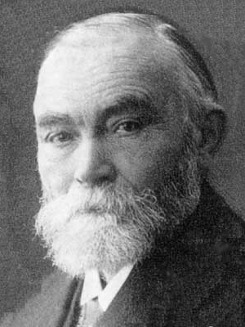
\includegraphics[width=0.6\textwidth]{frege.png}\\
    Gottlob Frege {\scriptsize\emph (Image by Wikipedia)}\\[3mm]
  \end{marginfigure}

  \begin{marginfigure}
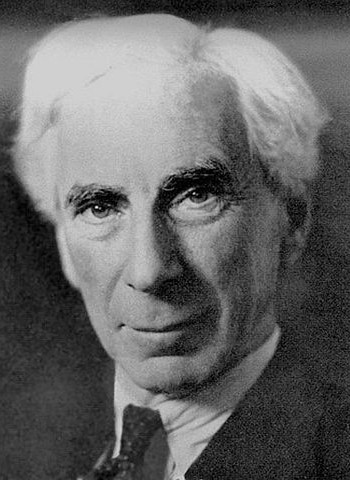
\includegraphics[width=0.6\textwidth]{russel.jpg}\\
    Bertrand Russell {\scriptsize\emph (Image by Wikipedia)}\\[3mm]
  \end{marginfigure}

\hspace{15pt}Door deze ontwikkeling introduceerde hij een nieuwe notatie en taal die de basis vormde van zijn werk en ten grondslag ligt aan de predikaatlogica die wij in deze reader zullen behandelen (zie hoofdstuk \ref{ch:predicaten}). Tot de aanpassingen van Boole en Frege was de logica, als mechanisme tot het onderzoeken en uitdrukken van het menselijk redeneren, niet verandert sinds zijn introductie door Aristoteles (circa 300 BC.).

\hspace{15pt}Frege's enorme werk werd verwoestend bekritiseerd door Bertrand Russell, die een fundamentele fout had gevonden in de zelf-evidente basis van Frege's werk (zie terzijde \ref{as:russel:paradox}). Echter werkte Russel vervolgens mee aan het repareren van deze kritieke fout, en verspreidde daarmee de idee\"en onder de Engelse wiskundigen (waaronder Boole, en later Turing en Church).
\footnotetext{Vrij naar `Logicomix -- An Epic Search for Truth', \citet{logicomix}.}
\end{aside}

\section{Metataal}\label{sec:metataal}
In deze reader behandelen wat bekend staat als `wiskundige logica', `symbolische logica' of `formele logica'\footnote{In tegenstelling tot `filosofische logica'.} Dat betekent dat we gebruik zullen maken van bekende wiskundige methoden om te onderzoeken wat logica inhoudt. Om deze context wat duidelijker te maken trekken we hier de vergelijking met een typische introductiecursus programmeren.

Een programmeercursus leert je niet alleen welke constructen uit de taal je kan gebruiken om bepaalde gevolgen te behalen als je het programma uitvoert, maar het leert je ook het verschil tussen de taal waarin je de programma's schrijft en de betekenis van die statements in termen van het effect ervan als ze worden uitgevoerd door de computer.
Als het een goede cursus zou zijn, dan zou ze je ook leren na te denken over programma's, bijvoorbeeld om in te zien dat twee verschillend lijkende programma's feitelijk hetzelfde zijn (of hetzelfde bereiken).

Logica is de studie van formele (symbolische) systemen van het redeneren en het bepalen van betekenis. Ze is vergelijkbaar met een introductie programmeren omdat beiden een analyse van formele systemen omvat als ook een analyse van betekenis (semantiek). Echter, in Logica bestudeer je veel meer diverse formele systemen dan in de informatica, zodat je logica niet alleen gebruikt als wiskundig middel voor de analyse, maar ook als fundament voor de wiskunde zelf. Dit zou de nodige alarmbellen moeten doen rinkelen, omdat we al hadden gezegd dat we wiskunde zouden gebruiken om Logica te bestuderen, dus we hebben te maken met een cirkelredenering (of \enquote{zelf-referentie}).

In de logica bestrijden we deze zelf-referentie door een duidelijk onderscheid te maken tussen de logica die we \underline{bestuderen} en de logica die we gebruiken om \underline{mee} te bestuderen. De logica die bestudeert wordt drukken we uit in een specifieke taal (de \emph{objecttaal}), terwijl de analyse van deze logica en taal uitgevoerd wordt in een andere taal (de \emph{metataal}).

Dit idee zou niet geheel vreemd voor je moeten zijn. Immers als je bijvoorbeeld Latijn zou bestuderen, zijn uitspraken in het Latijn in de objecttaal, terwijl de discussies die je voert over deze uitspraken in het Nederlands (de metataal). In de wiskunde is het niet anders (bijv., in calculus, verzamelingenleer, grafentheorie, etc.), maar ook in de informatica. In deze laatste is de objecttaal de taal waarin we programmeren, zoals Python, Java, Lisp, Miranda, en de metataal wederom Nederlands, mogelijk uitgebreid met wat toepasselijke wiskundige en informatica specifieke termen.

\begin{example}\mbox{}\\
Beschouw de volgende uitdrukking:
\begin{quote}\begin{texttt}times 0 do print * od = do\_nothing
\end{texttt}\end{quote}
\end{example}
Dit is, wezenlijk, een uitspraak in de metataal over de equivalentie van twee uitdrukkingen in een of andere programmeertaal. Wellicht had je het zelf ook al bedacht, maar het is bijzonder lastig om exact te bepalen welke symbolen tot de objecttaal en welke tot de metataal behoren. Figuur \ref{fig:metataal} geeft hierover verheldering.
\begin{figure}[h]
\begin{center}
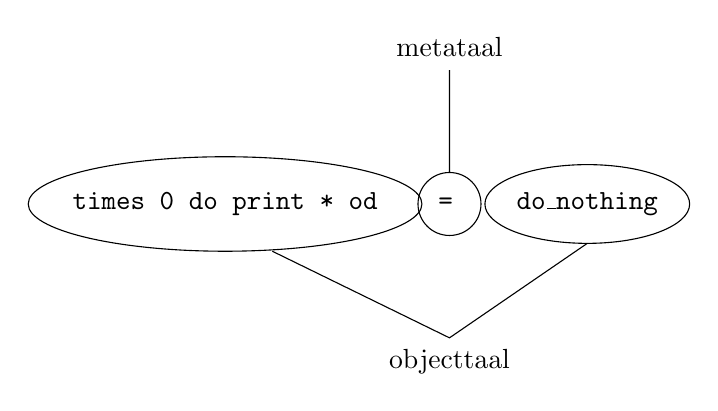
\begin{tikzpicture}
\node at (-0.1,0) {\tt times 0 do print * od};
\node at (2.7,0) {\tt =};
\node at (4.5,0) {\tt do\_nothing};
\draw (-0.1,0) ellipse (2.5cm and .6cm);
\draw (2.75,0) circle (.4cm);
\draw (4.5,0) ellipse (1.3cm and .5cm);
\node at (2.75, 2) {metataal};
\node at (2.75, -2) {objecttaal};
\draw (2.75,1.7) to (2.75,.4) (.5,-.6) to (2.75,-1.7) to (4.5,-.5);
\end{tikzpicture}
\caption{Onderscheid objecttaal en metataal.}\label{fig:metataal}
\end{center}
\end{figure}

Om correct te kunnen bepalen welke elementen tot welke taal behoren, is het noodzakelijk om een goede definitie te hebben van de objecttaal. Dit is het eerst dat we zullen doen in hoofdstuk \ref{ch:proposities}.

\section{Formalisatie}
Het proces van het opstellen van een objecttaal en het vaststellen van regels om deze te kunnen manipuleren noemen we \emph{formaliseren}. Het doel hiervan is om duidelijkheid te verkrijgen en fouten (misvattingen) te vermijden.

Een tweede, even belangrijke stap van het formaliseren is dat het formaliseren ons de mogelijkheid biedt om objecten te manipuleren zonder te hoeven begrijpen wat we precies aan het doen zijn. Dit klinkt als een stap achteruit, maar laten we een voorbeeld beschouwen: de rekenkunde volgt uit de formalisering van het tellen. Hierdoor hebben we nu regels die we kunnen volgen om getallen correct bij elkaar op te tellen zonder exact te weten wat de getallen zijn of wat optellen is.

De kracht van formaliseren is dan dat als er eenmaal geformaliseerd is, een gebied van interesse bewerkt kan worden zonder dat er begrip voor benodigd is. Zolang er goed is geformaliseerd en de gevonden regels strikt worden nageleefd, is begrip (intelligentie?) niet benodigd voor het uitvoeren van een taak. Zonder hier nu in een diepe filosofische discussie te belanden, hebben we hier zojuist de basis van machine intelligentie verklaard: computers kunnen, zonder begrip van de wereld, intelligente dingen doen, mits ze de juiste formalisaties krijgen aangereikt (d.w.z. wiskunde, logica, etc.) om die intelligente taken te kunnen volbrengen. Het is dus ook van dermate belang dat een AI'er bedreven is in de kunst van het formaliseren.

\section{Terminologie}
Tot slot, voor deze inleiding, rest ons nog de bespreking van enige terminologie die je in deze reader veelvuldig zal tegenkomen. Begrip van deze terminologie is essentieel voor het begrijpen van de aangeboden materie.

Belangrijke beweringen waarvoor een bewijs bestaat, wordt vaak een \textit{stelling} genoemd (Engels: \textit{theorem}). Een iets minder belangrijke bewering waarvoor een bewijs bestaat, wordt wel een \textit{propositie} genoemd (Engels: \textit{proposition}). Een bewering met een bewijs waarvan het belang niet op zich zelf staat, maar voornamelijk dient als hulpresultaat om een stelling te bewijzen, heet een \textit{lemma}. Een gevolg van een stelling wordt wel \textit{corollarium} genoemd (Engels: \textit{corrolary}). Het precies vastleggen van de betekenis van een nieuw begrip heet een \textit{definitie}. %Een fundamentele bewering die je niet bewijst maar als uitgangspunt hanteert heet een \textit{axioma}.

Bij een bewijs is het handig om te zien waar het begint en eindigt. Meestal begint het met het woord \textit{bewijs} (Engels: \textit{proof}, en eindigt het met een blokje $\square$). In sommige teksten wordt een bewijs afgesloten met de afkorting Q.E.D.. Dit staat voor \textit{quod erat demonstrandum}, hetgeen Latijn is voor "hetgeen bewezen moest worden". In dit dictaat hanteren wij een zwart blokje: $\blacksquare$.

Een bewering waarvan je verwacht dat die waar is, maar waarvoor geen bewijs gevonden is, heet een \textit{vermoeden} (Engels: \textit{conjecture}). Het is verbazend dat er veel eenvoudig te formuleren beweringen bestaan waarvan de juistheid wel vermoed wordt, en er is dan ook nooit een tegenvoorbeeld voor gevonden, maar waarvoor na uitgebreide inspanningen ook nog nooit een bewijs voor is gevonden.

  \begin{marginfigure}
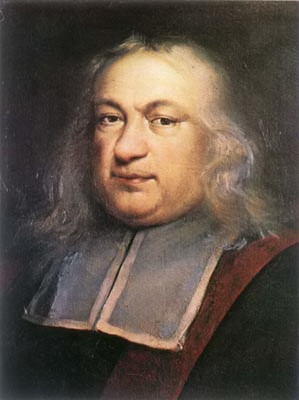
\includegraphics[width=0.6\textwidth]{Pierre_de_Fermat.jpg}\\
    Pierre de Fermat {\scriptsize\emph (Image by Wikipedia)}\\[3mm]
  \end{marginfigure}

\begin{aside}[Stelling van Fermat]\textbf{}\\[2.5pt]
Het komt ook wel voor dat dergelijke vermoedens toch nog bewezen worden. Een frappant voorbeeld hiervoor is de \textit{laatste stelling van Fermat}, rond 1637 door Fermat geformuleerd: \enquote{er bestaan geen gehele getallen $n>2$ en $a,b,c,>0$ waarvoor $a^n+b^n=c^n$}. Hoewel Fermat zelf beweerde hiervoor een wonderbaarlijk bewijs te hebben gevonden dat helaas te groot was om in de kantlijn op te nemen, is dat `bewijs' niet bewaard gebleven en is deze bewering honderden jaren een vermoeden geweest. Tot 1993: toen gaf Andrew Wiles hiervan een bewijs, dat compact opgeschreven enige honderden pagina's besloeg, exclusief de bewijzen van de vele gebruikte veelal zeer diepe al eerder bekende stellingen.
\end{aside}

\chapter{Propositielogica}\label{ch:proposities}
Als men wil gaan redeneren, dan is het belangrijk dat er bij de overdracht van een redenatie geen verandering ontstaat van hetgeen waarover men aan het redeneren is. Om ervoor te zorgen dat er geen misverstanden ontstaan over hetgeen dat iemand probeert uit te drukken, of de ander van te overtuigen, dient men te beschikken over een arsenaal van begrippen en uitdrukkingswijzen. Alleen wanneer men over deze zaken tot overeenstemming kan komen, bestaat er een redelijke kans dat twee of meer beoefenaars van een vak met elkaar kunnen praten zonder al te vaak in onzekerheid te verkeren over de betekenis van mededelingen die worden uitgewisseld.

Natuurlijke taal (dagelijkse spreektaal, zoals Nederlands of Engels) voldoet op dit vlak helaas niet, omdat natuurlijke taal niet precies genoeg is om verschillende interpretaties uit te sluiten. Een paar voorbeelden van zinnen die men in de krant zou kunnen lezen:
\begin{quote}
\enquote{niemand kan dit bijna doen}
\end{quote}
\begin{quote}
\enquote{kamer aangeboden voor student, tot 25 jaar}
\end{quote}
\begin{quote}
\enquote{wegens lekkage kerncentrale gesloten}
\end{quote}

Er bestaat in bovenstaande voorbeelden weinig kans op misverstanden omdat verkeerde (?) interpretatie onwaarschijnlijke situaties schetst. Echter\ldots het laatste bericht zou ook op de deur van een winkel kunnen hangen. En het is menigmaal voorgekomen dat een verdachte vrijgesproken is op grond van een onduidelijk gestelde beschuldiging.

Voorbeelden van een \enquote{vaktaal} in andere disciplines vinden we heel duidelijk in de protocollen van gerechtelijke uitspraken, en in notari\"ele akten. Ook daar heeft men gekozen voor bepaalde vaste formuleringen om de zaken ondubbelzinnig vast te leggen. Voor een buitenstaander wordt het daardoor echter meestal niet duidelijk, vaak is juist het tegendeel het geval!

De manier waarop iets is opgeschreven valt onder het begrip \textit{syntax}, de betekenis van het opgeschrevene valt onder het begrip \textit{semantiek}. We kunnen dus zeggen dat \enquote{zeven} en \enquote{7} syntactisch verschillend en semantisch hetzelfde zijn. Hier introduceren wij eerst de syntax van de propositielogica, de semantiek volgt later in sectie \ref{sec:wtab}.

\begin{aside}[Syntax vs. semantiek: De Jabberwocky]\mbox{}\\
Schrijver en logicus Lewis Carroll (1832 -- 1898) was erg geinteresseerd in de fenomenen taal en logica. Het is ook niet verwonderlijk dat hij in meerdere van zijn boeken logische puzzels verstopte en de relaties tussen taal en logica onderzocht.

E\'en zo'n voorbeeld is het Jabberwocky nonsensgedicht uit \textit{Through the Looking Glass, and What Alice Found There}, het vervolg op beroemde \textit{Alice's Adventures in Wonderland} \cite{carroll}. Carroll speelt hierin met het correct formuleren van taal (\emph{syntax}) en het cre\"eren van nonsense in betekenis (\emph{semantiek}). \\[2.5pt]

Engels origineel \cite{carroll}:
\begin{quote}
    'Twas brillig, and the slithy toves\\
    Did gyre and gimble in the wabe:\\
    All mimsy were the borogoves,\\
    And the mome raths outgrabe.
\end{quote}
Nederlandse vertaling\\ \cite{wauwelwok}:
\begin{quote}
    't Wier bradig, en de spiramants\\
	Bedroorden slendig in het zwiets:\\
	Hoe klarm waren de ooiefants,\\
	Bij 't bluifen der beriets.\\
\end{quote}

  \begin{marginfigure}
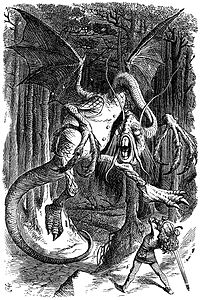
\includegraphics[width=0.6\textwidth]{jabberwocky.jpg}\\
   De Jabberwocky {\scriptsize\emph (Image by Wikipedia)}\\[3mm]
  \end{marginfigure}

Terwijl het gedicht in eerste oogopslag op een correct geformuleerd (Nederlands/Engels) gedicht lijkt, staat er in wezen niks dat betekenis vol is; alle woorden zijn correct gevormd (volgens fonetisch taalregels), maar hebben geen duidelijke betekenis\footnote{Het gedicht is nog briljanter omdat het door gebruik van onomatopees (klanknabootsingen) alsnog een boodschap weet over te brengen.}.
\end{aside}

Om het benodigde begrippenapparaat te introduceren om binnen de informatica (en wiskunde) precies te kunnen beschrijven wat er bedoelt wordt introduceren we nu het belangrijkste begrip van dit hoofdstuk.
\begin{definition}[Propositie]\label{def:prop}\mbox{}\\
Een \textit{propositie} is een zinvolle bewering, een vaststelling met een duidelijke betekenis: \textit{waar} \'of \textit{niet waar}.
\end{definition}

Het is erg lastig om een fundamenteel begrip zoals \enquote{propositie} ondubbelzinnig vast te leggen. Hoe objectief zijn \enquote{zinvol} en \enquote{duidelijk}? Wanneer we ons beperken tot de beweringen in een programmeertaal, dan is het tamelijk eenvoudig om precies te defini\"eren wat een propositie is, dat wil zeggen: hoe een propositie er syntactisch uitziet. We hebben dan wel een beperkte woordenschat, en kunnen gebruikmaken van de syntactische schema's die de programmeertaal defini\"eren. Wij zullen ons hier echter niet zo strikt vastleggen op de syntax, omdat we de theorie toepasbaar willen laten zijn op algemene onderwerpen uit wiskunde \`en informatica.

Voorbeelden van proposities zijn:
\begin{quote}
\begin{tabular}{p{.4\textwidth}p{.4\textwidth}}
\multicolumn{2}{l}{\enquote{in deze zaal zitten 140 mensen}}\\
\enquote{een plus een is twee}&\enquote{drie plus vijf is zes}\\
\enquote{de maan is een spiegel}&\enquote{$3+5=6$}\\
\enquote{dit bewijs is fout}&\enquote{$1-1=0$}
\end{tabular}
\end{quote}

We laten nu een paar voorbeelden zien van uitspraken die geen proposities zijn, en geven bij iedere uitspraak een kort commentaar tussen haakjes:
\begin{quote}
\begin{tabular}{p{.3\textwidth}p{.5\textwidth}}
\enquote{$x$ is gelijk aan $y$}&(niet duidelijk wat $x$ is en wat $y$ is)\\
\enquote{ga naar huis}&(geen vaststelling, maar een bevel)\\
\enquote{zou het regenen?}&(vragen zijn niet waar of onwaar; wel goed is \enquote{het regent})\\
\enquote{Jan te ver kaas}&(wat zou hiervan de betekenis zijn? Dit voldoet ook niet aan de syntax van de Nederlandse taal)
\end{tabular}
\end{quote}

Tenslotte nog een paar voorbeelden van uitspraken die wat complexer van aard zijn, en daarom meer aandacht vragen als het gaat om de vraag of het proposities zijn:
\begin{quote}\label{q:non:prop}
\enquote{alle mensen zijn dieren}\\
\enquote{als het gras nat wordt, dan regent het}\\
\enquote{Jan is een zoon van Kees en Mien is de moeder van Jaap}\\
\enquote{de zon schijnt of het regent}
\end{quote}

Een nieuwe element in bovenstaande uitspraken is dat er verschillende beweringen in \'e\'en uitspraak worden gedaan. We komen later hierop terug in sectie \ref{sec:samenstelling}.

In enkele van de voorbeelden zien we dat een propositie niet waar hoeft te zijn. In de definitie van het begrip propositie (definitie \ref{def:prop}) hebben we ge\"eist dat hij hetzij \textit{waar} hetzij \textit{onwaar} is (precies \'e\'en van beide). Dit betekent echter niet dat we over de waarheid onmiddellijk uitsluitsel moeten kunnen geven. Zo beschouwen we de uitspraak
\begin{quote}
\enquote{onder de eerste tien miljard decimalen van $\pi$ komen precies \'e\'en miljard cijfers $9$ voor}
\end{quote}
wel als een proposities. Immers, zij is waar of onwaar, maar we kunnen (nog) niet vaststellen of zij waar danwel onwaar is. Daarentegen is
\begin{quote}
\enquote{deze zin is onwaar}
\end{quote}
geen propositie. Immers, deze bewering kan niet waar zijn (want dan zegt zij zelf onwaar te zijn) en zij kan ook niet onwaar zijn (want dan zegt zij zelf waar te zijn). Men kan ook zeggen dat deze bewering zowel waar als onwaar is, maar naar onze begrippen is de betekenis van deze bewering niet duidelijk.

Merk op dat we gebruik hebben gemaakt van een nog onuitgesproken afspraak, die we nu expliciet zullen vastleggen.
\begin{axiom}\label{ax:dubbel}
\enquote{niet onwaar} betekent hetzelfde als \enquote{waar}.
\end{axiom}
Dit axioma (een fundamentele afspraak) is een hoeksteen van de klassieke logica. Hierdoor wordt het mogelijk om een bewijs uit het ongerijmde te vormen: als de ontkenning van de propositie onwaar is, dan is de propositie zelf waar!

\begin{aside}[Constructieve logica]\mbox{}\\[1em]
Niet alle filosofen zijn het eens over het gebruik van axioma \ref{ax:dubbel} in de klassieke logica. De Nederlandse filosoof en wiskundige Luitzen Brouwer formuleerde een logica, \textit{intu\"itionistische logica}, waarin dit axioma niet als uitgangspunt werd genomen (sterker nog, in intu\-\"itionistische logica is de propositie die wordt uitgedrukt door axioma \ref{ax:dubbel} niet te bewijzen en dus onwaar).

  \begin{marginfigure}
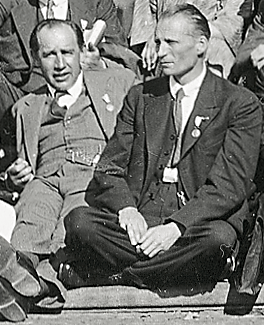
\includegraphics[width=0.6\textwidth]{Bohr_Brouwer.png}\\
    Luitzen Brouwer (rechts) {\scriptsize\emph (Image by Wikipedia)}\\[3mm]
  \end{marginfigure}
 
\hspace{15pt}Intu\"itionistische logica wordt gerekend tot de stroming van het \textit{constructivisme} (of constructieve wiskunde), omdat voor elk stelling een bewijs moet worden gemaakt (geconstrueerd); d.w.z., een stelling is alleen `waar' als er bewezen kan worden dat deze waar is. Het gebruik van bewijzen uit het ongerijmde (waarmee men bewijst dat een stelling `waar' is door te bewijzen dat zijn ontkenning `onwaar' is) is niet toegestaan.

Intu\"itionistische logica wordt veelal toegepast in de correctheid bewijzen van algoritmes binnen de informatica.
\end{aside}

% In het vervolg zullen we de betekenis van een propositie vernauwen tot het waar danwel onwaar zijn van de propositie.
In het vervolg zullen we met de betekenis van een propositie bedoelen of deze waar of onwaar is.

\section{Samenstellen van proposities}\label{sec:samenstelling}
Het kunnen opschrijven van proposities die waar danwel onwaar zijn geeft ons een krachtige basis, maar we willen ook kunnen redeneren over combinaties. Zoals in sommige voorbeelden al te zien was (zie pagina \pageref{q:non:prop}) is het wenselijk dat we proposities kunnen samenstellen. Wat we zouden willen is dat zo'n samenstelling zelf ook weer een propositie zou worden. Daarvoor is nodig dat de samenstelling ook voldoet aan de definitie van propositie (definitie \ref{def:prop}), en dus moeten we precies vastleggen wat we bedoelen met uitspraken als
\begin{quote}
\enquote{\ldots en \ldots}\\
\enquote{\ldots of \ldots}\\
\enquote{als\ldots dan\ldots}\\
\enquote{\ldots dan, en slechts dan, als\ldots}\\
\enquote{niet \ldots}
\end{quote}
waarin op de plaats van de stippeltjes proposities kunnen  worden ingevuld.

Een eerste stap in het vastleggen van een notatie voor deze samenstellingen. Het is niet verstandig om hiervoor alleen het gewone woordgebruik te kiezen. Immers, aan het begin van dit hoofdstuk hebben we al gezien dat hierdoor misverstanden kunnen ontstaan bij de interpretatie. Daarnaast heeft het invoeren van een compacte notatie het voordeel dat ingewikkeldere uitdrukkingen die we daarmee kunnen opbouwen, nog steeds betrekkelijk compact opgeschreven kunnen worden.
\begin{notation}\mbox{}\\
Laten $p$ en $q$ proposities voorstellen. We gebruiken de volgende notaties:\\

  \noindent\parbox{2cm}{$p\land q$} voor \enquote{$p$ en $q$}\\
  \noindent\parbox{2cm}{$p\lor q$} voor \enquote{$p$ of $q$}\\
  \noindent\parbox{2cm}{$p\rightarrow q$} voor \enquote{als $p$ dan $q$} of \enquote{$q$ als $p$}\\
  \noindent\parbox{2cm}{$p\leftrightarrow q$} voor \enquote{$p$ dan, en slechts dan, als $q$}\sidenote{De uitspraak \enquote{$p$ dan en slechts dan als $q$} wordt vaak afgekort tot \enquote{$p$ desda $q$} of \enquote{$p$ iff $q$} (naar het Engels: \enquote{$p$ if and only if $q$}).}\\
  \noindent\parbox{2cm}{$\neg p$} voor \enquote{niet $p$}\\


\noindent
De symbolen $\land$, $\lor$, $\rightarrow$, $\leftrightarrow$, $\neg$ heten \textit{connectieven}, of ook wel \textit{Boolse operatoren}. Ze staan respectievelijk bekend onder de namen \textit{conjunctie}, \textit{disjunctie}, \textit{implicatie}, \textit{bi-implicatie} en \textit{negatie}.
\end{notation}

\subsection{Opgaven}
\begin{exercise}[Proposities]\mbox{}\\
Welke van de volgende uitspraken is een propositie en welke niet?
\begin{enumerate}[label=\textit{\alph*.}]
\item $7+7 = 13$.
\item $7+7 = 14$.
\item Er bestaan groene koeien.
\item Er bestaat leven op een andere planeet.
\item Het schilderij \textit{De Nachtwacht} van Rembrandt is mooi.
\item Koning Willem-Alexander vindt het schilderij \textit{De Nachtwacht} van Rembrandt mooi.
\item Het schilderij \textit{De Nachtwacht} van Rembrandt is mooier dan het schilderij \textit{De Zonnebloemen} van Van Gogh.
\item Het schilderij \textit{De Nachtwacht} van Rembrandt is zwaarder dan het schilderij \textit{De Zonnebloemen} van Van Gogh.
\item Deze zin bestaat uit meer dan twintig letters.
\end{enumerate}
\end{exercise}

\begin{exercise}[Vertalen]\mbox{}\\
Vertaal de volgende zinnen in propositielogica:
\begin{enumerate}[label=\textit{\alph*.}]
\item Als Jan droomt dan slaapt hij.
\item Slapen is een noodzakelijke voorwaarde voor dromen.
\item Niet drinken is een voldoende voorwaarde om niet dronken te worden.
\item Als ik gedronken heb en toch autorijd, dan loop ik kans op een forse boete.
\item Als ik gedronken heb en toch autorijd, dan loop ik kans op een forse boete, behalve als het promillage alcohol in mijn bloed onder een bepaalde waarde ligt.
\item Als ik autorijd en ik ben dronken of onder invloed van XTC dan maak ik de weg onveilig.
\end{enumerate}
\end{exercise}

\section{Waarheidstabellen}\label{sec:wtab}
Nu we hebben vastgesteld hoe we samenstellingen van proposities kunnen schrijven (syntax), moeten we deze nog voorzien van een betekenis (semantiek). Omdat de uitspraken $p$ en $q$ proposities zijn, is hun betekenis per definitie duidelijk: waar of niet waar. Omdat er maar twee mogelijkheden zijn kunnen we de betekenis van een samenstelling vastleggen door voor alle mogelijke waarden van $p$ en $q$ het resultaat vast te leggen. We doen dit met behulp van \textit{waarheidswaarde}\footnote{In de filosofie en wiskunde wordt de waarheid van een propositie vaak aangeduid met de symbolen $T$ (true = waar) en $F$ (false = onwaar). Deze komen vaak in die vorm terug in wetenschappelijke papers. Wij volgen echter de notatie uit de informatica die aansluit bij activatie van logische gates (hoog = $1$ = waar; laag = $0$ = onwaar).} en \textit{waarheidstabellen}.

\begin{definition}[Waarheidswaarde]\mbox{}\\
De waarheidswaarde van een propositie is 0 of 1:\\
\indent een propositie die waar is, heeft waarheidswaarde 1,\\
\indent een propositie die onwaar is, heeft waarheidswaarde 0.
\end{definition}

Vervolgens stellen we de zogenaamde \textit{waarheidstabellen} op: we sommen systematisch alle combinaties van waarheidswaarden van $p$ en $q$ op, en geven bij elke samenstelling aan wat het gewenste resultaat is. 
%
\begin{fullwidth}
$$
\begin{array}{ccc}
p&q&p\land q\\
\hline
0&0&0\\
0&1&0\\
1&0&0\\
1&1&1
\end{array}\quad 
\begin{array}{ccc}
p&q&p\lor q\\
\hline
0&0&0\\
0&1&1\\
1&0&1\\
1&1&1
\end{array}\quad
\begin{array}{ccc}
p&q&p\rightarrow q\\
\hline
0&0&1\\
0&1&1\\
1&0&0\\
1&1&1
\end{array}\quad
\begin{array}{ccc}
p&q&p\leftrightarrow q\\
\hline
0&0&1\\
0&1&0\\
1&0&0\\
1&1&1
\end{array}\quad
\begin{array}{cc}
p&\neg p\\
\hline
0&1\\
1&0\\
&\\
&
\end{array}
  $$\\[5mm]
\end{fullwidth}
%
Deze tabellen kunnen  gezien worden als een compact opgeschreven definitie van alle samenstellingen.

Als we willen weten hoe de waarheidswaarde van bijvoorbeeld $p\land q$ afhangt van de waarheidswaarden van $p$ en $q$, dan vergelijken we de kolommen van $p$ en $q$ met de kolom van $p\land q$ en lezen de gewenste informatie horizontaal af. Hieruit zien we dan de definitie van $p\land q$:
\begin{definition}[Conjunctie]\label{def:conj}\mbox{}\\
De propositie $p\land q$ is waar als $p$ en $q$ beide waar zijn. In alle andere gevallen is $p\land q$ onwaar.
\end{definition}

Analoog hebben we de definitie van $p\lor q$:
\begin{definition}[Disjunctie]\label{def:disj}\mbox{}\\
De propositie $p\lor q$ is onwaar als $p$ en $q$ beide onwaar zijn. In alle andere gevallen is $p\lor q$ waar.
\end{definition}

Hetzelfde kunnen we doen met $\neg p$:
\begin{definition}[Negatie]\label{def:neg}\mbox{}\\
De propositie $\neg p$ is waar als $p$ onwaar is en onwaar als $p$ waar is.
\end{definition}

De definities van deze operatoren komt overeen met de logische gates die eerder (in Computer Systemen en Netwerken) zijn besproken: het $\land$-symbool werkt hetzelfde als een AND-gate, het $\lor$-symbool werkt hetzelfde als een OR-gate en het $\neg$-symbool werkt hetzelfde als een INVERT- of NOT-gate.

Voor het volgende symbool is het wenselijk om wat uitvoeriger stil te staan bij de betekenis. Uit de tabel zien we:
\begin{definition}[Implicatie]\label{def:impl}\mbox{}\\
De propositie $p\rightarrow q$ is onwaar als $p$ waar en $q$ onwaar is. In alle andere gevallen is $p\rightarrow q$ waar.
\end{definition}

Een consequent van deze definitie van $p\rightarrow q$ is dat er voor de waarheid van $p\rightarrow q$ \textit{geen verband} tussen $p$ en $q$ vereist is. Als we dus voor $p$ en $q$ twee ware proposities invullen, die niets met elkaar te maken hebben, dan is $p\rightarrow q$ een ware uitspraak. Zo'n ware uitspraak is bijvoorbeeld:
\begin{quote}
$1=1$ $\quad\rightarrow\quad$ Python is een programmeertaal
\end{quote}

Het is \textit{af te raden} om $p\rightarrow q$ uit te spreken als \enquote{uit $p$ volgt $q$}: geldigheid van $p\rightarrow q$ zegt alleen dat $q$ waar is als $p$ waar is, en niet dat daarbij sprake is van een oorzakelijk verband\footnote{Voor het concept \enquote{uit\ldots volgt\ldots} gebruikt men in de logica een semantisch symbool: $\vdash$. In hoofdstuk \ref{ch:bewijzen} komen we hier nog op terug.}.

Een andere consequentie is dat $p\rightarrow q$ altijd waar is als $p$ onwaar is. Nu vinden we dat misschien niet zo erg vreemd, omdat we een uitspraak als
\begin{quote}
\enquote{Als Pasen en Pinksteren op \'e\'en dag vallen, dan\ldots}
\end{quote}
niet als een leugen opvatten, ook al zou er op de plaats van de stippeltjes iets onwaars staan. Plastisch gezegd: uit een absurde veronderstelling kan men alles concluderen. Toch zal menigeen de wenkbrauwen fronsen bij het lezen van de ware uitspraak
$$e=\pi\quad\rightarrow\quad 1=1$$

\noindent Soortgelijke opmerkingen kunnen worden gemaakt over de samenstelling $p\leftrightarrow q$.
\begin{definition}[Bi-implicatie]\label{def:bi}\mbox{}\\
De propositie $p\leftrightarrow q$ is waar als de waarheidswaarde van $p$ dezelfde is als die van $q$. In alle andere gevallen is $p\leftrightarrow q$ onwaar.
\end{definition}

We kunnen samenstellingen van proposities natuurlijk opnieuw samenstellen en daarmee ingewikkelde constructies maken, zoals bijvoorbeeld
$$(p\land q)\rightarrow r$$
$$(p\rightarrow q)\rightarrow p$$
$$((\neg p\rightarrow q)\land(\neg q\rightarrow p))\leftrightarrow (p\leftrightarrow\neg q)$$
die allen weer proposities zijn. Hierbij gebruiken we haakjes om de opbouw duidelijk te maken.

Veel haakjes zijn overbodig als er (bijvoorbeeld door de syntax) afspraken gemaakt worden over de prioriteit van de connectieven. De enige regel die wij hierover expliciet vastleggen is dat de negatie $\neg$ sterker bindt dan alle andere connectieven; d.w.z. $\neg p\land q$ dient men te lezen als $(\neg p)\land q$ en niet als $\neg(p \land q)$. Wat betreft de overige connectieven bestaan er verschillende regels, maar deze zullen wij bewust niet hanteren; het loont altijd om, als er verwarring kan ontstaan, haakjes te gebruiken. 

Van dit soort combinaties kunnen we ook weer waarheidstabellen maken: som weer alle mogelijkheden voor $p$ en $q$ systematisch op en bereken wat het resultaat is. Omdat we dat voor elke van de connectieven al hadden vastgelegd, ligt het resultaat voor elke daarmee opgebouwde combinatie ook vast.

\subsection{Andere connectieven}
In de natuurlijke taal komen nog andere connectieven voor dan alleen de zojuist behandelde. Zo kennen we bijvoorbeeld uitdrukkingen als 
\begin{quote}
\enquote{noch\ldots, noch\ldots}\\
\enquote{\`of\ldots, \`of\ldots}\\
\enquote{wel\ldots, maar niet\ldots}
\end{quote}

Aangezien de waarheidstabel van een connectief dat twee proposities $p$ en $q$ verbindt uit vier regels bestaat, zijn er dus 16 verschillende manieren om een waarheidstabel voor zo'n connectief te construeren: op elke plek kunnen we een $1$ of een $0$ zetten. Daaronder komen ook de connectieven voor die alleen iets met $p$ of alleen iets met $q$ of die helemaal onafhankelijk zijn van $p$ en $q$. Van deze laatste zijn er twee; ze worden de weergegeven met $\top$ en $\bot$. De waarheidswaarde van $\top$ is in alle gevallen $1$, en de waarheidswaarde van $\bot$ is in alle gevallen $0$. $\top$ staat daarmee voor de universele waarheid (ook wel `top' genoemd of `truth'); $\bot$ is de universele onwaarheid (ook wel `bottom' of `falsum' genaamd). Soms worden ze ook wel aangeduid als $\mathbf{T}$ en $\mathbf{F}$. Je zou kunnen denken dat $\top$ hetzelfde is als $1$ en $\bot$ hetzelfde als $0$, maar dat is niet helemaal waar: $\top$ en $\bot$ zijn proposities en $1$ en $0$ zijn waarden. Je kan dus zeggen dat $\top$ (of $\mathbf{T}$) en $\bot$ (of $\mathbf{F}$ tot de \textit{syntax} van proposities, net als alle connectieven, en dat $0$ en $1$ de \textit{semantiek} weergeven van respectievelijk $\top$ en $\bot$.
\begin{aside}[Top $\top$ / bottom $\bot$]\mbox{}\\
Propositielogica is vrij eenvoudig en onderscheidt maar \textit{vier} verschillende unieke waardes:
\begin{enumerate}
\item iets dat altijd waar is (universele waarheid: $\top$);
\item iets dat altijd onwaar is (universele onwaarheid: $\bot$);
\item iets dat een bepaalde waarheidswaarde heeft, maar die nu nog niet bekend is, bijvoorbeeld $p$; en
\item de negatie van die propositie $\neg p$.
\end{enumerate}

\noindent
Zoals we later zullen zien, in sectie \ref{sec:equiv}, zijn deze waardes niet in elkaar uit te drukken. Bijvoorbeeld, $\top$ zal nooit hetzelfde zijn als $\bot$ (iets dat altijd waar is, zal nooit onwaar zijn), en omgekeerd. Datzelfde geldt voor $p$ en $\neg p$; d.w.z. een propositie zal nooit dezelfde waarheidswaarde hebben als zijn negatie. Het verschil tussen $\top$ en $p$ (of $\neg p$), en zo ook tussen $\bot$ en $p$ (of $\neg p$) liggen wat genuanceerder (dit zal duidelijker worden in sectie \ref{sec:equiv}); kort gezegd drukt \enquote{iets dat mogelijk waar of onwaar is} (dus $p$) iets anders uit dan \enquote{hetgeen dat altijd waar is} (dus $\top$).

Deze vier verschillende waardes kunnen klassiek gerelateerd worden in een lattice (een raster):
\begin{center}
\begin{tikzpicture}
\node at (0,1) (p) {$p$};
\node at (1,2) (top) {$\top$};
\node at (2,1) (negp) {$\neg p$};
\node at (1,0) (bot) {$\bot$};
\draw (top) -- (p);
\draw (top) -- (negp);
\draw (p) -- (bot);
\draw (negp) -- (bot);
\end{tikzpicture}
\end{center}
De universele waarheid is hiermee de `top' van het raster, en de universele onwaarheid is de `bottom'; vandaar de benaming `top' en `bottom' en het gebruik van $\top$ en  $\bot$ als symbolen voor deze begrippen.
\end{aside}

In de waarheidstabellen hiervoor hebben we maar 5 van de 16 mogelijkheden getoond, enerzijds omdat juist die de connectieven zijn waarvan gebruik wordt gemaakt in redeneringen, anderzijds omdat elke samengestelde propositie reeds kan worden geformuleerd met de connectieven $\land$, $\lor$ en $\neg$\footnote{Sterker nog, alleen $\land$ en $\neg$ (of $\lor$ en $\neg$) zijn voldoende om alle connectieven af te leiden; zie ook sectie \ref{sec:volledig}.}. Een paar voorbeelden:
\begin{quote}
$p\rightarrow q$ heeft dezelfde waarheidstabel als $\neg p\lor q$.\\
\enquote{noch $p$, noch $q$} heeft dezelfde waarheidstabel als $\neg p\land\neg q$.
\end{quote}
We komen hier nog uitgebreid op terug in sectie \ref{sec:equiv}.

\begin{aside}[Andere connectieven]\label{as:andere:conn}\mbox{}\\
Een aantal van de meest bekende connectieven die \textit{niet} standaard in propositielogica worden gedefinieerd (maar gek genoeg wel vaak terugkomen in de informatica) zijn de XOR, de NOR en de NAND.\\[2.5pt]
\hspace{15pt}
De `exclusieve or'-operator (XOR) is ingevoerd als vertaling voor \enquote{\`of\ldots, \`of\ldots} en wordt meestal geschreven als $\oplus$, als $\veebar$ of als $\mathrel{\ooalign{$\leftrightarrow$\cr\hidewidth$/$\hidewidth}}$. Ze werkt hetzelfde als de XOR-gate, en is de tegenhanger van de equivalentie-operator ($\leftrightarrow$, vergelijk de waarheidstabellen!).

  \begin{marginfigure}
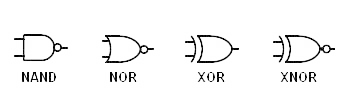
\includegraphics[trim={.5cm 0 4cm 0},clip,width=\textwidth]{gates.png}
  \end{marginfigure}

De `not and'-operator (NAND), ook wel \textbf{Sheffer Stroke} genaamd, wordt in de logica geschreven als $\uparrow$ en werkt hetzelfde als de NAND-gate (zie ook de waarheidstabel hieronder). Ze kan ook worden uitgedrukt als $\neg(p\land q)$.

De `not or'-operator (NOR) is haar directe tegenhanger (zie ook de waarheidstabel), en is in de logica ook wel bekend als \textbf{Peirce Arrow} of \textbf{Quine Dagger}. Ze wordt geschreven als $\downarrow$ en werkt vergelijkbaar als de NOR-gate. Ze kan ook worden uitgedrukt als $\neg(p\lor q)$ (zie ook de waarheidstabellen).

Een markant detail is dat zowel de Sheffer Stroke als de Quine Dagger \textit{op zichzelf} voldoende is om alle andere connectieven af te kunnen leiden (zie sectie \ref{sec:volledig}).
$$\begin{array}{ccc}
p&q&p\oplus q\\
\hline
0&0&0\\
0&1&1\\
1&0&1\\
1&1&0
\end{array}\quad
\begin{array}{ccc}
p&q&p\uparrow q\\
\hline
0&0&1\\
0&1&1\\
1&0&1\\
1&1&0
\end{array}\quad
\begin{array}{ccc}
p&q&p\downarrow q\\
\hline
0&0&1\\
0&1&0\\
1&0&0\\
1&1&0
\end{array}
$$
\end{aside}

\subsection{Opgaven}
\begin{exercise}[Waarheidstabellen]\mbox{}\\
Construeer de waarheidstabellen van de volgende samengestelde proposities:
\begin{enumerate}[label=\textit{\alph*.}]
\item $(p\land q)\land((\neg q)\lor r)$
\item $p\rightarrow(q\lor r)$
\item $\neg((\neg p)\lor\neg((\neg q)\lor\neg p))$
\item $p\leftrightarrow(q\leftrightarrow r)$
\item $p\leftrightarrow(q\leftrightarrow p)$
\end{enumerate}
\end{exercise}

\section{Metaredeneren}
%\todo[inline,color=hured!40]{Logisch gevolg, onderscheid syntax/semantiek, equivalentie, meta-beweringen}
Logica analyseert niet alleen bestaande vormen van redeneren, maar probeert ook de eigenschappen van die systemen te analyseren. De propositielogica is daarvan een uitstekend voorbeeld; het kan gebruikt worden om stelselmatige wetmatigheden te bestuderen.

Logici zijn al eeuwen ge\"interesseerd in `speciale' formules, bijvoorbeeld $p\lor\neg p$ en $p\land\neg p$. De eerste is immers nooit onwaar, de tweede is nooit waar. Deze eigenschappen van formules kunnen we afleiden uit de waarheidstabellen van de formule, en we kunnen uitzoeken welke eigenschappen van de waarheidstabellen van de formule in kwestie hiervoor verantwoordelijk zijn.

Een andere wetmatigheid heeft te maken met redeneringen. Waarom vinden we dat een redenering van de vorm `uit $p\lor\neg q$ en $q$ kan men $p$ afleiden' correct (geldig), en welke eigenschappen van de waarheidstabellen van de formules in kwestie zijn hiervoor verantwoordelijk.

Door op zo'n wiskundige manier te denken kunnen we dus precies defini\"eren wat geldigheid is, maar kunnen we hiermee ook allerlei mooie patronen zien in geldig redeneren die anders onzichtbaar zouden blijven. Voorbeelden die we zullen zien zijn de dualiteit van conjunctie en disjunctie in de aanwezigheid van negatie, en het systematisch aan elkaar schakelen van implicaties.

Deze vorm van redeneren over het redenatie-systeem (oftewel eigenschappen proberen te ontlenen aan de wetmatigheden van de logica) wordt ook wel meta-redeneren genoemd (redeneren over het redeneren). Hoewel het soms erg verwarrend kan zijn (beide zijn immers redenaties) is het uiterst belangrijk om uitspraken op het meta-niveau te onderscheiden van uitspraken op het redenatie-niveau (vergelijk met metataal vs. objecttaal in sectie \ref{sec:metataal}). Dit onderscheid vindt zijn grondslag in het verschil tussen de syntax en de semantiek van de propositielogica. Uitspraken over geldigheid, het gevolg van redeneringen, etc., hebben allen betrekking op de semantiek (betekenis) van de logica, en dienen derhalve dus te worden uitgedrukt in symbolen die anders zijn de de symbolen die worden gebruikt om de argumenten te noteren (de syntax). 

\subsection{Tautologie\"en}
Sommige proposities zijn steeds waar, andere zijn soms waar en soms onwaar, afhankelijk van de situatie waarop ze betrekking hebben. Zo is \enquote{de brug is open} waar als de brug open is, en anders is deze uitspraak onwaar. Wanneer men in een computerprogramma twee variabelen $x$ en $y$ heeft, dan is de als test te gebruiken propositie \enquote{$x=y$} waar als $x$ en $y$ dezelfde waarde hebben, en anders onwaar. De propositie \enquote{$x=x$} is echter altijd waar.

Wat ons vooral interesseert zijn samengestelde proposities en hoe men aantoont dat een propositie steeds waar is. Bij een uit een klein aantal proposities $p, q, r,\ldots$ samengestelde propositie $A$ kan men gemakkelijk controleren of $A$ steeds waar is door de waarheidstabel van $A$ op te stellen en te kijken of de waarheidswaarde van $A$ steeds $1$ is. De elementaire bouwstenen $p, q, r,\ldots$ heten wel \textit{atomen} of \textit{atomaire proposities}. Omdat elk atoom twee waarheidswaarden kan hebben, bestaat de waarheidstabel voor een proposities opgebouwd uit $n$ verschillende atomen uit $2^n$ regels. Voor een $n=3$ of $n=4$ is dat nog best te doen, maar als $n$ minstens $10$ is, zijn er toch wel minstens duizend regels nodig, en komt de vraag op of het niet met minder werk kan.

We zullen nu een manier aangeven om te manipuleren met samengestelde proposities, het vervangen van een propositie door een andere propositie met dezelfde betekenis. Met dergelijke manipulaties is het opstellen en nalopen van waarheidstabellen vaak te vermijden.

Twee proposities $A$ en $B$, beide opgebouwd uit $p, q, r,\ldots$, hebben dezelfde betekenis precies dan als $A\leftrightarrow B$ steeds waar is. Dit is hetzelfde als zeggen dat de waarheidstabellen van $A$ en $B$ aan elkaar gelijk zijn.

\begin{definition}[Tautologie]\mbox{}\\
Een \textit{tautologie} is een steeds ware propositie, oftewel voor elke keuze van waarheidswaarden voor de erin voorkomende atomen is de waarheidswaarde van de propositie $1$.
\end{definition}
%
Een propositie is dus een tautologie als hij dezelfde waarheidstabel heeft als $\top$.

Hieronder volgt een lijstje van belangrijke tautologie\"en, zodat we die niet telkens weer opnieuw hoeven te bewijzen. De in de lijst voorkomende letters zijn atomen. Hiervoor mag men willekeurige concrete proposities invullen (ook samengestelde proposities) onder de voorwaarde dat voor dezelfde propositieletter ook steeds dezelfde (samengestelde) propositie wordt ingevuld.

\begin{theorem}\mbox{}\\
Alle proposities in de volgende lijst zijn tautologie\"en:
\begin{enumerate}
\item $p\lor\neg p$
\item $\neg(p\land\neg p)$
\item $p\rightarrow(q\rightarrow p)$
\item $\neg p\rightarrow(p\rightarrow q)$
\item $(p\land\neg p)\rightarrow q$
\item $(p\leftrightarrow q)\rightarrow(p\rightarrow q)$
\item $((p\rightarrow q)\land(q\rightarrow r))\rightarrow(p\rightarrow r)$
\item $(p\rightarrow q)\lor(q\rightarrow p)$
\item $(p\rightarrow q)\rightarrow((q\rightarrow r)\rightarrow(p\rightarrow r))$
\item $((p\rightarrow q)\land(r\rightarrow s))\rightarrow((p\land r)\rightarrow(q\land s))$
\item $((p\rightarrow q)\lor(r\rightarrow s))\rightarrow((p\land r)\rightarrow(q\lor s))$
\item $((p\leftrightarrow q)\land(q\leftrightarrow r))\rightarrow(p\leftrightarrow r)$
\item $\top$
\item $\neg\bot$
\end{enumerate}
\end{theorem}

Het lijkt een lange lijst, maar de regels 1 t/m 6 liggen nogal voor het oprapen. Regel 7 drukt uit dat implicatie \textit{transitief} is. Hopelijk geven regels 8 en 11 de lezer het gevoel dat het niet allemaal zo vanzelfsprekend is.

Een stelling is pas echt een stelling als er ook een bewijs bij is; in dit geval betekent dat dat we voor elke regel moeten bewijzen dat de genoemde propositie een tautologie is. Dat kunnen we met waarheidstabellen doen: als we systematisch alle mogelijke combinaties van waarheidswaarden voor $p, q$ en $r$ afgaan en zien dat de waarheidswaarde van de propositie in alle gevallen $1$ is, hebben we bewezen dat het een tautologie is. Dit doen we hier alleen voor regel 7; voor de overige regels gaat het op soortgelijke wijze en laten we het aan de lezer over. Voor regel 7 moeten we laten zien dat $((p\rightarrow q)\land(q\rightarrow r))\rightarrow(p\rightarrow r)$ een tautologie is, en daarvoor moeten we eerst de waarheidswaarden van $p\rightarrow q$, van $q\rightarrow r$, van $(p\rightarrow q)\wedge(q\rightarrow r)$ en van $p\rightarrow r$ bepalen. Dat zouden we afzonderlijk kunnen doen door hier aparte waarheidstabellen van te maken, maar het kan ook in \'e\'en keer met een grote waarheidstabel, waarin we onder de pijl van $p\rightarrow q$ de waarheidswaarde van $p\rightarrow q$ noteren, vervolgens onder de pijl van $q\rightarrow r$ de waarheidswaarde van $q\rightarrow r$, enzovoorts:
\begin{proof} $((p\rightarrow q)\land(q\rightarrow r))\rightarrow(p\rightarrow r)$ is een tautologie:
\begin{center}
\begin{tikzpicture}[node distance=1mm and 0mm,baseline]
\matrix (M1) [matrix of nodes, column sep=1em]
{
  $p$ & $q$ & $r$ & $((p\rightarrow q)$ & $\land$ & $(q\rightarrow r))$ & $\rightarrow\ $ & $(p\rightarrow r)$ \\
  0 & 0 & 0 & 1 & 1 & 1 & 1 & 1 \\
  0 & 0 & 1 & 1 & 1 & 1 & 1 & 1\\
  0 & 1 & 0 & 1 & 0 & 0 & 1 & 1 \\
  0 & 1 & 1 & 1 & 1 & 1 & 1 & 1 \\
  1 & 0 & 0 & 0 & 0 & 1 & 1 & 0 \\
  1 & 0 & 1 & 0 & 0 & 1 & 1 & 1 \\
  1 & 1 & 0 & 1 & 0 & 0 & 1 & 0 \\
  1 & 1 & 1 & 1 & 1 & 1 & 1 & 1 \\
};
\draw (M1-1-1.south west) -- (M1-1-8.south east);
\draw (M1-1-1.north west) -- (M1-9-1.south west) -- (M1-9-8.south east -| M1-1-8.east) -- (M1-1-8.north east);
\draw[hublue, ultra thick] (M1-1-7.north west) rectangle (M1-9-7.south east);
\end{tikzpicture}
\end{center}
\end{proof}
Inderdaad zien we in de rood omrande kolom alleen maar enen staan, waarmee bewezen is dat de hele propositie een tautologie is.

In principe maakt de volgorde van de mogelijke combinaties van waarheidswaarden niet uit, als alle mogelijke combinaties maar opgesomd worden. Hier is de systematiek gevolgd waarbij het laatste atoom ($r$) afwisselend 0 en 1 is ingevuld, bij het voorlaatste ($q$) afwisselend twee nullen en twee enen, en daar weer voor (bij $p$) eerst vier nullen en dan vier enen. Dit breidt op een voor de hand liggende manier uit naar elk willekeurig aantal atomen: bij $n$ atomen staan er in de eerste $n$ kolommen de getallen van 0 tot en met $2^n-1$ in \textit{binaire notatie}.

Twee hieraan verwante begrippen die nog ge\"introduceerd dienen te worden zijn \textit{contradictie} en \textit{contingentie}.
\begin{definition}[Contradictie]\mbox{}\\
Een \textit{contradictie} is een steeds onware propositie, oftewel voor elke keuze van waarheidswaarden voor de erin voorkomende atomen is de waarheidswaarde van de propositie $0$.
\end{definition}
Een propositie is dus een contradictie als hij dezelfde waarheidstabel heeft als $\bot$.
\begin{definition}[Contingentie]\mbox{}\\
Een \textit{contingentie} is een propositie die soms waar en soms onwaar is, oftewel voor enkele keuzes van waarheidswaarden voor de erin voorkomende atomen (maar voor tenminste \'e\'en) is de waarheidswaarde van de propositie $1$ \'en voor enkele keuzes van waarheidswaarden voor de erin voorkomende atomen (maar voor tenminste \'e\'en) is de waarheidswaarde van de propositie $0$.
\end{definition}
Een propositie is dus een contingentie als hij noch een tautologie, noch een contradictie is.

\subsection{Equivalenties}\label{sec:equiv}
Hoewel het maken van een waarheidstabel een eenvoudige (doch bewerkelijke) exercitie is, kan het in het geval dat een samengestelde propositie veel atomen bevat toch gauw uit de klauw lopen. Zoals eerder genoemd is voor het maken van een waarheidstabel van een propositie met $n$ verschillende atomaire proposities een waarheidstabel benodigd met $2^n$ rijen.

Gelukkig zijn er effectievere methoden om te bepalen of de waarheidstabellen van twee proposities gelijk aan elkaar zijn. Hiervoor introduceren wij het begrip \textit{equivalentie}.
%
\begin{definition}[Equivalentie]\mbox{}\\
Twee proposities $A$ en $B$ heten \textit{gelijkwaardig} of \textit{equivalent} als $A\leftrightarrow B$ een tautologie is, oftewel voor elke keuze van waarheidswaarden voor de erin voorkomende atomen is de waarheidswaarde van $A$ gelijk aan die van $B$.

\noindent
We schrijven dan wel $A\equiv B$, of ook wel $A\Leftrightarrow B$\footnote{Bemerk hier ook weer het onderscheid tussen \textit{syntax} en \textit{semantiek}: $A\leftrightarrow B$ drukt syntactisch uit dat $A$ en $B$ equivalent zijn, zoals gedefinieerd voor het geldende connectief (zie definitie \ref{def:bi}). $A\equiv B$ of $A\Leftrightarrow B$ drukken \textit{semantisch} uit dat de \textit{waarde van $A$} hetzelfde is als de \textit{waarde van $B$}.}.
\end{definition}

In de volgende tabel presenteren wij een aantal veel voorkomende en gebruikte equivalenties. Het nut van zo'n tabel is dat deze je basispatronen biedt die je kan gebruiken om complexe samengestelde proposities te vereenvoudigen.

\begin{theorem}
De proposities in de volgende lijst zijn op eenzelfde regel gelijkwaardig aan elkaar\\
$\begin{array}{*7l}
1. & p & \neg(\neg p) & p\land p\quad{} & p\lor p & p\lor\bot\quad{} & p\land\top \\
2. & p\lor q & q\lor p \\
3. & p\land q & q\land p\\
4. & p\leftrightarrow q & q\leftrightarrow p & \multicolumn{2}{l}{(p\rightarrow q)\land(q\rightarrow p)} & \multicolumn{2}{l}{(p\land q)\lor(\neg p \land\neg q)} \\
5. & (p\lor q)\lor r & p\lor(q\lor r) \\
6. & (p\land q)\land r & p\land(q\land r) \\
7. & p\rightarrow q & \neg p\lor q & \neg q \rightarrow\neg p \\
8. & \neg(p\rightarrow q) & p\land\neg q \\
9. & \neg(p\lor q) & \neg p\land\neg q \\
10. & \neg(p\land q) & \neg p \lor\neg q \\
11. & (p\lor q)\land r & \multicolumn{2}{l}{(p\land r)\lor(q\land r)} \\
12. & (p\land q)\lor r & \multicolumn{2}{l}{(p\lor r)\land(q\lor r)} \\
13. & (p\lor q)\rightarrow r & \multicolumn{2}{l}{(p\rightarrow r)\land(q\rightarrow r)} \\
14. & p\rightarrow(q\land r) & \multicolumn{2}{l}{(p\rightarrow q)\land (p\rightarrow r)} \\
15. & p\rightarrow(q\rightarrow r) & (p\land q)\rightarrow r \\
16. & p\lor\neg p & p\lor\top & \top \\
17. & p\land\neg p & p\land\bot & \bot 
\end{array}$\label{th:equiv}
\end{theorem}

Regels 2, 3 en 4 (eerste deel) geven aan dat de operatoren $\lor$, $\land$, en $\leftrightarrow$ \textit{commutatief} zijn. Regels 5 en 6 geven aan dat de operatoren $\lor$ en $\land$ \textit{associatief} zijn. Regel 7 geeft eigenlijk de definitie van de implicatie en tevens de contrapositie. Regels 8, 9 en 10 laten zien hoe we met ontkenningen moeten omgaan. Regels 9 en 10 staan bekend als de \textit{wetten van De Morgan}.

Regels 11 en 12 beschrijven dat $\lor$ en $\land$ \textit{distributief} zijn, preciezer: regel 11 zegt dat $\land$ \textit{distribueert over} $\lor$, en regel 12 zegt dat $\lor$ distribueert over $\land$. Regel 16 en 17 geven nog enkele voordehandliggende verbanden met $\top$ en $\bot$.

Van deze lijst is het handig om in ieder geval regels 1 t/m 12 en 16, 17 te kennen en altijd paraat te hebben.

Ook deze stelling kan zonder enig probleem worden bewezen door voor de onderhavige proposities de waarheidstabellen op te stellen en te controleren dat de zaak klopt: steeds moet je laten zien dat proposities op dezelfde regel precies gelijke kolommen geven in de waarheidstabel. Nadat de equivalenties uit de stelling zijn bewezen, echter, kan je deze toepassen om complexe samenstellingen te vereenvoudigen.

Voor het toepassen van Stelling \ref{th:equiv} zijn de volgende opmerkingen van groot belang:
\begin{itemize}
\item Voor $p, q, r,\ldots$ mogen steeds willekeurige proposities worden ingevuld;
\item De regels zijn niet alleen van toepassing op de hele uitdrukking, maar ook op delen daarvan. Zo mogen we uit $A\equiv B$ concluderen: $\neg A\equiv\neg B$, $p\lor A\equiv p\lor B$, $A\lor p\equiv B\lor p$, $p\land  A\equiv p\land B$, et cetera.
\end{itemize}

Het op deze wijze toepassen van Stelling \ref{th:equiv} en andere spelregels van dit hoofdstuk wordt soms ook wel \textit{propositierekening} of \textit{equivalentierekenen} genoemd.

Een dergelijke methode kan ook worden gebruikt om andere regels van Stelling \ref{th:equiv} te bewijzen. Als voorbeeld laten we zien hoe regel 10 van Stelling \ref{th:equiv} volgt uit andere regels door proposities te vervangen door gelijkwaardige proposities\footnote{Voor de hier gebruikte regels 1, 7 en 9 dient natuurlijk ook een bewijs te worden gegeven, bijv. door middel van een waarheidstabel. Dit laten wij hier aan de lezer over.}. Een dergelijk bewijs heet een \textit{equitioneel bewijs}.
\begin{proof}\mbox{}\\
$\begin{array}{llll}
\neg(p\rightarrow q) & \equiv & \neg(\neg p\lor q) & \text{(regel 7)}\\
& \equiv & \neg(\neg p)\land\neg q & \text{(regel 9)} \\
& \equiv & p\land\neg q & \text{(regel 1)}
\end{array}$\\
\end{proof}

Op deze manier kunnen we ook nieuwe gelijkwaardigheden worden afgeleid, bijvoorbeeld\\
$\begin{array}{llll}
p\land(q\lor r) & \equiv & (q\lor r)\land p & \text{(regel 3)} \\
& \equiv & (q\land p)\lor(r\land p) & \text{(regel 11)} \\
& \equiv & (p\land q)\lor(r\land p) & \text{(regel 3)} \\
& \equiv & (p\land q)\lor(p\land r) & \text{(regel 3)}
\end{array}$

Door herhaaldelijk toepassen van de regels 2 en 5 van Stelling \ref{th:equiv} kan men laten zien dat in $p\lor q\lor\ldots\lor r$ de haakjes willekeurig geplaatst mogen worden, en dat de volgorde er niet toe doet. Daarom laten we in samenstellingen met alleen het connectief $\lor$ vaak de haakjes weg.

Eenzelfde opmerking geldt voor $p\land q\land\ldots\land r$, hetgeen volgt door herhaaldelijk toepassen van regels 3 en 6.

\subsection{Logisch Gevolg}
Met de hier ontwikkelde begrippen zijn we nu in staat om een precieze logische definitie te geven van wat we intu\"itief een correcte redenering noemen. Welke eigenschap van de waarheidstabellen van de betrokken formules is hiervoor verantwoordelijk?

Om dit te achterhalen, beschouwen we een eenvoudige redenering: uit `Jan is een goede schaker en Karin een goede dammer' kan worden geconcludeerd: `Jan is een goede schaker'. Het uitgangspunt is `Jan is een goede schaker en Karin is een goede dammer' en de conclusie is `Jan is een goede schaker'. Hier is geen speld tussen te krijgen: de redenering is correct. Zij nu $p =$ `Jan is een goede schaker' en $q =$ `Karin is een goede dammer'. We maken vervolgens de waarheidstabellen van het uitgangspunt (premisse) $(p\land q)$ en de conclusie $p$:\\
\begin{tikzpicture}[node distance=1mm and 0mm,baseline]
\matrix (M) [matrix of nodes, column sep=1em]
{
  $p$ & $q$ & $p\land q$ & $p$ \\
  0 & 0 & 0 & 0 \\
  0 & 1 & 0 & 0 \\
  1 & 0 & 0 & 1 \\
  1 & 1 & 1 & 1 \\
};
\draw (M-1-1.south west) -- (M-1-4.south east);
\draw (M-1-1.north west) -- (M-5-1.south west) -- (M-5-4.south east -| M-1-4.east) -- (M-1-4.north east);
\draw[hublue,ultra thick] (M-1-3.north west) rectangle (M-5-3.south east -| M-1-3.east);
\draw[hublue,ultra thick] (M-1-4.north west) rectangle (M-5-4.south east);
\end{tikzpicture}

Vergelijken we de aangegeven kolommen, dan valt op dat het uitgangspunt en de conclusie niet altijd tegelijk waar zijn, en niet dezelfde waarheidswaarde hoeven te hebben, maar dat, en dit is essentieel:
\begin{quote}
als het uitgangspunt waar is, dan is ook de conclusie waar.
\end{quote}
We spreken van \textit{logisch gevolg} of van `geldige gevolgtrekking'.

\begin{definition}[Logisch gevolg]\label{def:gevolg}
De formule $\psi$ is een logisch gevolg van $\varphi_1,\ldots,\varphi_n$ als elke waardering die alle $\varphi_1,\ldots,\varphi_n$ waar maakt, ook $\psi$ waar maakt.\\
We schrijven hiervoor $\varphi_1,\ldots,\varphi_n\Rightarrow\psi$ of $\varphi_1,\ldots,\varphi_n\therefore\psi$.
\end{definition}

\begin{example}
De redenering in het vorige voorbeeld kunnen we weergeven als $p\land q\therefore p$, dat wil zeggen: $p$ is een logisch gevolg van $p\land q$. Immers, er was blijkens de tabel maar \'e\'en waardering die $p\land q$ waar maakte (de laatste regel), en die maakt inderdaad de conclusie $p$ ook waar.\\
In dit voorbeeld is $n=1$ en $\varphi_1$ de formule $p\land q$.
\end{example}

\begin{example}
Gegeven is de volgende redenering:
\begin{quote}
`De afstandsbediening is kapot of de tv werkt niet goed. Maar de tv werkt wel goed. Dus de afstandsbediening is kapot.'
\end{quote}
We kiezen nu $p=$ `De afstandsbediening is kapot' en $q=$ `De tv werkt goed'. We gaan nu kijken of $p$ een logisch gevolg is van $p\lor\neg q$ en $q$ samen.\\
\begin{tikzpicture}
\matrix (M) [matrix of nodes, column sep=1em] {
    $p$ & $q$ & $\neg q$ & $p\lor\neg q$ & $q$ & $p$ \\
    0 & 0 & 1 & 1 & 0 & 0 \\
    0 & 1 & 0 & 0 & 1 & 0 \\
    1 & 0 & 1 & 1 & 0 & 1 \\
    1 & 1 & 0 & 1 & 1 & 1 \\
};
\draw (M-1-1.south west) -- (M-1-6.south east);
\draw (M-1-1.north west) -- (M-5-1.south west) -- (M-5-6.south east -| M-1-6.east) -- (M-1-6.north east);
\draw[hublue,ultra thick] (M-5-4.north west) rectangle (M-5-4.south east);
\draw[hublue,ultra thick] (M-5-5.north west) rectangle (M-5-5.south east);
\end{tikzpicture}

\noindent
Uit de tabel blijkt dat de beide uitgangspunten alleen tegelijk waar zijn (omrandde enen) als $p$ en $q$ waar zijn (laatste regel). Met andere woorden: we hoeven slechts naar de laatste rij waarheidswaarden te kijken, en daar is de conclusie ook waar. Kortom: $p\lor\neg q,q\therefore p$. In dit voorbeeld is $n=2$, $\varphi_1$ de formule $p\lor\neg q$ en $\varphi_2$ de formule $q$.
\end{example}

Merk op dat in de definitie van geldig gevolg staat: \textit{elke} waardering die de uitgangspunten waar maakt, moet de conclusie waar zijn. Het is niet voldoende dat er \textit{een} waardering bestaat die zowel uitgangspunten als conclusie waar maakt.

\begin{example}\label{ex:no:gevolg}
Uit `Er komen meer wegen in Nederland precies dan als Nederland geasfalteerd raakt' is niet correct te concluderen dat er meer wegen in Nederland komen. Formeel $p\leftrightarrow q\not\therefore p$, dat wil zeggen, $p$ is geen logisch gevolg van $p\leftrightarrow q$. Er is \textit{een} waardering die het uitgangspunten en de conclusie waarmaakt, namelijk de waardering die $p$ en $q$ allebei waarmaakt. Maar er is ook een waardering die $p\leftrightarrow q$ waarmaakt, maar niet de conclusie, namelijk de waardering die $p$ en $q$ allebei onwaar maakt.\\
\begin{tikzpicture}
\matrix (M) [matrix of nodes, column sep=1em] {
    $p$ & $q$ & $p \leftrightarrow q$ & $q$  \\
    0 & 0 & 1 & 0 \\
    0 & 1 & 0 & 1 \\
    1 & 0 & 0 & 0 \\
    1 & 1 & 1 & 1 \\
};
\draw (M-1-1.south west) -- (M-1-4.south east);
\draw (M-1-1.north west) -- (M-5-1.south west) -- (M-5-4.south east -| M-1-4.east) -- (M-1-4.north east);
\draw[hublue,ultra thick] (M-5-3.north west) rectangle (M-5-3.south east);
\draw[hublue,ultra thick] (M-5-4.north west) rectangle (M-5-4.south east);
\draw[hublue,ultra thick] (M-2-3.north west) rectangle (M-2-3.south east);
\draw[hublue,ultra thick] (M-2-4.north west) rectangle (M-2-4.south east);
\node at (2.5,-.85) {\color{green!70!black}{\usym{2714}}};
\node at (2.5,.35) {\color{red}{\large\usym{2718}}};
\end{tikzpicture}
\end{example}

Een aantal bekende vormen van gevolgtrekkingen zijn:\\
\begin{tabular}{|p{4cm}p{6cm}|}
\hline
\textit{naam}&\textit{vorm van de gevolgtrekking}\\
&\\
uitgesloten derden&$\neg\neg\varphi\therefore\varphi$\\
modus ponens&$\varphi,\varphi\rightarrow\psi\therefore\psi$\\
contrapositie&$\varphi\rightarrow\psi\therefore\neg\psi\rightarrow\neg\varphi$\\
hypothetisch syllogisme&$\varphi\rightarrow\psi,\psi\rightarrow\chi\therefore\varphi\rightarrow\chi$\\
\hline
\end{tabular}\label{tab:gevolg}\vspace{2mm}

Deze regels worden (vaak stilzwijgend) gebruikt bij wiskundige bewijzen.

\begin{aside}[Symbool voor logisch gevolg]\mbox{}\\
Logisch gevolg wordt, in verschillende bronnen, uitgedrukt door middel van verschillende symbolen: $\vdash$, $\vDash$ of $\therefore$.

Het symbool $\vdash$ werd voor het eerst gebruikt door Gottlob Frege in zijn \textit{Begriffschrifft} (\citeyear{frege:begriffschrift}) om \textit{afleidbaarheid} aan te duiden. Het wordt klassiek gelezen als \enquote{maakt waar}, \enquote{bewijst dat}, \enquote{vervult} of \enquote{brengt met zich mee}. Het symbool zelf wordt ook wel \textbf{turnstile} (draaihekje) genoemd, omdat het er enigszins op lijkt (van boven gezien). Het wordt soms ook \textbf{tee} genoemd. Het is het universele symbool voor \textit{beweringen}, waarbij $\vdash A$ gelezen wordt als \textit{ik weet dat $A$ waar is} (of \textit{uit niets is $A$ af te leiden}). Soortgelijk leest men afhankelijke beweringen als $P\vdash Q$ als \textit{vanuit $P$ weet ik dat $Q$} (ofwel, \textit{gegeven $P$ weet ik dat $Q$}, of \textit{gegeven $P$ kan ik $Q$ afleiden}).

De semantische tegenhanger is de dubbele turnstile $\vDash$, welke wordt gebruikt om semantisch gevolg aan te duiden; als alles aan de linkerzijde van het symbool waar is, dan moet de bewering aan de rechterzijde ook waar zijn, bijv. $\Gamma\vDash A$. Merk op dat dit erg verwant is aan de enkele turnstile, die syntactisch gevolg aanduidt (uit de syntactische beweringen links zijn de beweringen rechts af te leiden). $\vDash$ geeft hiermee \textit{vervulbaarheid} aan, terwijl $\vdash$ \textit{afleidbaarheid} aanduidt... maar we begrijpen dat dit verschil voor de meesten erg minimaal is en lastig te onderscheiden.

Het dus-teken $\therefore$ tenslotte, is een logisch en wiskundig symbool gebruikt in bewijzen om een gevolg (conclusie) aan te duiden. Je zou het in een redenering kunnen vervangen door het woordje `dus'. Omdat het een semantische betekenis heeft (je koppelt de betekenis van de beweringen aan elkaar om tot een conclusie te komen), is ze verwant aan $\vDash$. Merk overigens op dat ze de tegenhanger is van het \textit{omdat-teken} ($\because$).
\end{aside}

\subsection{Opgaven}
\begin{exercise}\mbox{}\\
Bewijs met behulp van waarheidstabellen dat
\begin{enumerate}[label=\textit{\alph*.}]
\item $((p\rightarrow q)\lor(r\rightarrow s))\rightarrow((p\land r)\rightarrow(q\lor s))$ een tautologie is.
\item $((p\rightarrow q)\land(q\rightarrow r))\rightarrow(p\rightarrow r)$ een tautologie is.
\item $\neg(p\rightarrow\neg q)$ en $p\land q$ gelijkwaardig zijn.
\end{enumerate}
\end{exercise}

\begin{exercise}\mbox{}\\
Bewijs door gebruik te maken van één van de gelijkwaardige proposities uit Stelling \ref{th:equiv}, dat de onderstaande paren van proposities gelijkwaardig aan elkaar zijn. De eerste is voorgedaan.
\begin{enumerate}[label=\textit{\alph*.}]
% a:
\item $\neg ((d\leftrightarrow e)\vee d)$ en $\neg (d\leftrightarrow e) \wedge \neg d$ \\
antwoord:
\begin{align}
\neg ((d\leftrightarrow e)\vee d) &\equiv \neg (d\leftrightarrow e)\wedge \neg d  \tag{St-\ref{th:equiv}: 9}
\end{align}
%b:
\item $(e\land h) \leftrightarrow b$ en $((e\land h) \land b) \lor (\neg (e\land h)\land \neg b)$
%c:
\item $(a\lor (b\rightarrow a)) \rightarrow z$ en $(a\rightarrow z)\land ((b\rightarrow a) \rightarrow z)$
%d:
\item $(p\land \neg e)\lor (\neg e \rightarrow q)$ en $(\neg e\rightarrow q)\lor (p\land \neg e)$
%e:
\item $a \leftrightarrow (b\rightarrow a)$ en $a \leftrightarrow (\neg a\rightarrow \neg b)$ 
%f:
\item $(h \land (f\lor z))\rightarrow q$ en $h\rightarrow ((f\lor z) \rightarrow q)$  
%g:
\item $\neg (p\leftrightarrow q)\lor \neg z$ en $\neg ((p\leftrightarrow q) \land z)$  
%h:
\item $q \rightarrow \neg \neg (h \leftrightarrow z) $ en $q \rightarrow (h \leftrightarrow z)$ 
\end{enumerate}
\end{exercise}

\begin{exercise}\mbox{}\\
Bewijs door gebruik te maken van twee of meer van de gelijkwaardige proposities uit Stelling \ref{th:equiv}, dat de onderstaande paren van proposities gelijkwaardig aan elkaar zijn. De eerste is voorgedaan.
\begin{enumerate}[label=\textit{\alph*.}]
% a:
\item $(\neg b\land a)\lor \neg (a\lor \neg b)$ en $a\leftrightarrow \neg b$\\
antwoord:
\begin{align}
(\neg b\wedge a)\vee \neg (a\vee \neg b) &\equiv (\neg b\wedge a)\vee (\neg a \wedge \neg \neg b)  \tag{St-\ref{th:equiv}: 9} \\
&\equiv (a\wedge \neg b)\vee (\neg a \wedge \neg \neg b)  \tag{St-\ref{th:equiv}: 3} \\
&\equiv a\leftrightarrow \neg b\tag{St-\ref{th:equiv}: 4}
\end{align}
% b:
\item $z\land ((q\rightarrow e) \lor (q\rightarrow e))$ en $(q \rightarrow e) \land z$
% c:
\item $\neg (m\land h)$ en $m \rightarrow \neg h$
% d:
\item $(n \lor r)\rightarrow (p \land r)$ en $((n \lor r)\rightarrow p) \land (\neg r \rightarrow \neg (n \lor r))$
% e:
\item $\neg (\neg a \rightarrow z)$ en $\neg a \land \neg (\neg z\rightarrow z)$
% f:
\item $\neg(p\rightarrow q) \lor (\neg (q \rightarrow p) \lor r)$ en $\neg (p\leftrightarrow q) \lor r$
% g:
\item $(z\lor k)\rightarrow m$ en $(\neg z \lor m) \land (\neg k \lor m)$
% h:
\item $c \land (h\leftrightarrow d)$ en $\neg (c \rightarrow \neg (d \leftrightarrow h))$  

\end{enumerate}
\end{exercise}

\begin{exercise}\mbox{}\\
Bewijs dat regels 13, 14 en 15 van Stelling \ref{th:equiv} inderdaad gelijkwaardige proposities aangeven.
\end{exercise}

\begin{exercise}\mbox{}\\
Bewijs door uitsluitend te vervangen door gelijkwaardige proposities uit Stelling \ref{th:equiv}, dat
\begin{enumerate}[label=\textit{\alph*.}]
\item $a\leftrightarrow b$ en $\neg a \leftrightarrow \neg b$ gelijkwaardig zijn.
\item $(\neg a\land\neg b)\rightarrow c$ en $\neg a\rightarrow(b\lor c)$ gelijkwaardig zijn.
\end{enumerate}
\end{exercise}

\begin{exercise}\mbox{}\\
Oom Henk heeft altijd de grootste verhalen. Zijn jonge neefjes en nichtjes zijn meer van \enquote{goed verhaal, lekker kort}. Nu wil oom Henk graag wat propositielogica aan zijn neefjes en nichtjes laten zien, maar ook bij zijn propositielogica heeft hij last van zijn breedsprakigheid. Help oom Henk met hip zijn en versimpel de onderstaande propositie zo veel mogelijk  Er is er al één voorgedaan. 
\begin{enumerate}[label=\textit{\alph*.}]
% a:
\item $\neg ((a\land b) \lor \neg(\neg a \rightarrow b))$\\
antwoord:
\begin{align}
\neg ((a\wedge b)\vee \neg (\neg a\rightarrow b)) &\equiv \neg (a\wedge b) \wedge \neg \neg (\neg a\rightarrow b)  \tag{St-\ref{th:equiv}: 9} \\
&\equiv \neg (a\wedge b) \wedge (\neg a\rightarrow b)   \tag{St-\ref{th:equiv}: 1} \\
&\equiv (\neg a \vee \neg b) \wedge (\neg a\rightarrow b) \tag{St-\ref{th:equiv}: 10} \\
&\equiv (\neg a \vee \neg b) \wedge (\neg a\rightarrow \neg \neg b) \tag{St-\ref{th:equiv}: 1} \\
&\equiv (\neg a \vee \neg b) \wedge (\neg b \rightarrow a) \tag{St-\ref{th:equiv}: 7} \\
&\equiv (a \rightarrow \neg b) \wedge (\neg b \rightarrow a) \tag{St-\ref{th:equiv}: 7} \\
&\equiv a \leftrightarrow \neg b \tag{St-\ref{th:equiv}: 4}
\end{align}
% b:
\item $\neg (p \rightarrow \neg (q \rightarrow q))$
% c:
\item $\neg((\neg p\rightarrow q)\rightarrow ((p\rightarrow\neg r)\wedge(r\rightarrow q)))$
\end{enumerate}
\end{exercise}

\begin{exercise}\mbox{}\\
Bepaal voor alle volgende stellingen of het altijd, soms of nooit een logisch gevolg is (maak zo nodig een waarheidstabel om te checken):
\begin{enumerate}[label=\textit{\alph*.}]
\item $\varphi\vdash\psi$ als $\varphi$ en $\psi$ beiden een tautologie zijn;
\item $\varphi\vdash\psi$ als $\varphi$ een tautologie is en $\psi$ een contradictie;
\item $\varphi\vdash\psi$ als $\varphi$ een tautologie is en $\psi$ een contingentie;
\item $\varphi\vdash\psi$ als $\varphi$ een contradictie is en $\psi$ een tautologie;
\item $\varphi\vdash\psi$ als $\varphi$ een contradictie is en $\psi$ een contradictie;
\item $\varphi\vdash\psi$ als $\varphi$ een contradictie is en $\psi$ een contingentie;
\item $\varphi\vdash\psi$ als $\varphi$ een contingentie is en $\psi$ een tautologie;
\item $\varphi\vdash\psi$ als $\varphi$ een contingentie is en $\psi$ een contradictie;
\item $\varphi\vdash\psi$ als $\varphi$ een contingentie is en $\psi$ een contingentie;
\end{enumerate}
\end{exercise}

\section{Functionele compleetheid}\label{sec:volledig}
%\begin{remark}
%De stof in deze sectie behoort niet tot de basisstof van het vak en zal niet getentamineerd worden. Ze is enkel toegevoegd voor ge\"interesseerde studenten die \textit{verder} willen dan de gemiddelde student.
%\end{remark}
Aan het einde van sectie \ref{sec:wtab} hebben we aangekondigd dat elk connectief zich laat schrijven met behulp van de connectieven $\land$, $\lor$ en $\neg$. Inderdaad, laat $A$ een propositie zijn, opgebouwd uit eindig veel $p, q, r, \ldots$. Dan stellen we van $A$ de waarheidstabel op, en kijken hoe de waarheidswaarden van $p, q, r, \ldots$ moeten zijn opdat $A$ de waarheidswaarde $1$ heeft. We inventariseren die waarden met $\land$ en $\neg$ voor elke rij waarin $A$ de waarde $1$ staat. Het totaal wordt vervolgens samengevoegd met $\lor$. We krijgen op die manier vanzelf een uitdrukking in $p,q,r,\ldots$ en $\land,\lor,\neg$ (en haakjes, uiteraard).

Als voorbeeld nemen we $A(p,q,r,s)$ met de volgende waarheidstabel:
\begin{center}
\begin{tikzpicture}[node distance=1mm and 0mm,baseline]
\matrix (M1) [matrix of nodes, column sep=1em]
{
  $p$ & $q$ & $r$ & $s$ & $A$ \\
  0 & 0 & 0 & 0 & 0 \\
  0 & 0 & 0 & 1 & 0 \\
  0 & 0 & 1 & 0 & 0 \\
  0 & 0 & 1 & 1 & 0 \\
  0 & 1 & 0 & 0 & 0 \\
  0 & 1 & 0 & 1 & 1 \\
  0 & 1 & 1 & 0 & 0 \\
  0 & 1 & 1 & 1 & 0 \\
  1 & 0 & 0 & 0 & 0 \\
  1 & 0 & 0 & 1 & 1 \\
  1 & 0 & 1 & 0 & 0 \\
  1 & 0 & 1 & 1 & 1 \\
  1 & 1 & 0 & 0 & 0 \\
  1 & 1 & 0 & 1 & 0 \\
  1 & 1 & 1 & 0 & 0 \\
  1 & 1 & 1 & 1 & 0 \\
};
\draw (M1-1-1.south west) -- (M1-1-5.south east);
\draw (M1-1-4.north east) -- (M1-17-4.south east);
\draw (M1-1-1.north west) -- (M1-17-1.south west) -- (M1-17-5.south east -| M1-1-5.east) -- (M1-1-5.north east);
\draw[hublue,thick] (M1-7-1.north west) rectangle (M1-7-5.south east);
\draw[hublue,thick] (M1-11-1.north west) rectangle (M1-11-5.south east);
\draw[hublue,thick] (M1-13-1.north west) rectangle (M1-13-5.south east);
\end{tikzpicture}
\end{center}
%
Dan is $A(p,q,r,s)$ gelijkwaardig met
$$(p\land\neg q\land r\land s)\lor(\neg p\land q\land\neg r\land s)\lor(p\land\neg q\land\neg r\land s)$$
Dit is een zogenaamde \textit{disjunctieve normaalvorm} van $A$, oftewel een disjunctie van een aantal conjuncties van literals. Hierbij wordt onder een \textit{literal} verstaan een van de uitdrukkingen $p, \neg p, q, \neg q, r, \neg r,\ldots$, oftewel een atoom met al dan niet een ontkenning ervoor.

\begin{definition}[Disjunctieve normaalvorm]\mbox{}\\
Een \textit{disjunctieve normaalvorm} van een propositie opgebouwd uit de atomen $p_1,p_2,\ldots,p_r$ is een equivalente propositie van de vorm $X_1\lor X_2\lor\ldots\lor X_s$, waarbij elke $X_i$ van de vorm $(Y_1\land Y_2\land\ldots\land Y_{n_i})$ is, en elke $Y_j$ van de vorm $p_k$ of $\neg p_k$ is voor een zekere $k$.
\end{definition}

Een propositie kan meer dan \'e\'en disjunctieve normaalvorm hebben: zo is $p\lor(q\land r)$ zelf als een disjunctieve normaalvorm, maar levert de methode met de waarheidstabel hiervoor een equivalente disjunctieve normaalvorm die een disjunctie van vijf conjuncten is.

Ook zonder gebruik te maken van waarheidstabellen kan men een disjunctieve normaalvorm van een samengestelde propositie opstellen, namelijk via een equationeel bewijs. Dit kan heel systematisch door alleen de volgende equivalenties van links naar rechts toe te passen:
\begin{eqnarray*}
p\leftrightarrow q & \equiv & (p\land q)\lor (\neg p\land\neg q) \\
p\rightarrow q & \equiv & \neg p\lor q \\
\neg(\neg p) & \equiv & p \\
\neg(p\lor q) & \equiv & \neg p\land\neg q \\
\neg(p\land q) & \equiv & \neg p\lor\neg q \\
p\land(q\lor r) & \equiv & (p\land q)\lor(p\land r) \\
(p\lor q)\land r & \equiv & (p\land r)\lor(q\land r)
\end{eqnarray*}
Al deze regels komen voor of volgen direct uit Stelling \ref{th:equiv}. Desgewenst mogen we onderweg de betreffende uitdrukking nog vereenvoudigen door toepassing van regels 1, 16, 17 van Stelling \ref{th:equiv}. We geven een voorbeeld: we willen een disjunctieve normaalvorm van $(p\leftrightarrow q)\land(q\rightarrow r)$ bepalen:
\begin{eqnarray*}
(p\leftrightarrow q)\land(q\rightarrow r) 
  & \equiv & ((p\land q)\lor(\neg p\land\neg q))\land(q\rightarrow r) \\
  & \equiv & ((p\land q)\lor(\neg p\land\neg q))\land(\neg q\lor r) \\
  & \equiv & (p\land q\land(\neg q\lor r))\lor(\neg p\land\neg q\land(\neg q\lor r)) \\
  & \equiv & (p\land q\land\neg q)\lor(p\land q\land r)\lor(\neg p\land\neg q\land(\neg q\lor r)) \\
  & \equiv & (p\land\bot)\lor(p\land q\land r)\lor(\neg p\land\neg q\land(\neg q\lor r)) \\
  & \equiv & \bot\lor(p\land q\land r)\lor(\neg p\land\neg q\land(\neg q\lor r)) \\
  & \equiv & (p\land q\land r)\lor(\neg p\land\neg q\land(\neg q\lor r)) \\
  & \equiv & (p\land q\land r)\lor(\neg p\land \neg q\land\neg q)\lor(\neg p\land\neg q\land r) \\
  & \equiv & (p\land q\land r)\lor(\neg p\land\neg q)\lor(\neg p\land\neg q\land r)
\end{eqnarray*}
$(p\land q\land r)\lor(\neg p\land\neg q)\lor(\neg p\land\neg q\land r)$ is dus een disjunctieve normaalvorm van $(p\leftrightarrow q)\land(q\rightarrow r)$. Het kan nog korter: vanwege $(\neg p\land\neg q)\lor(\neg p\land\neg q\land r)\equiv\neg p\land\neg q$ is ook $(p\land q\land r)\lor(\neg p\land\neg q)$ een disjunctieve normaalvorm van $(p\leftrightarrow q)\land(q\rightarrow r)$.

Door directe controle of door de regels 1 en 9 van stelling \ref{th:equiv} te combineren, ziet men dat $p\lor q$ gelijkwaardig is met $\neg(\neg p\land\neg q)$. Daarmee blijkt uit de disjunctieve normaalvorm dat elke propositie gelijkwaardig is met een uitdrukking in alleen $\neg$ en $\land$. We laten het aan de lezer over om aan te tonen dat ook de paren $\lor$, $\neg$ en $\rightarrow$, $\neg$ voldoende zijn (zie opgaven). Zo'n set van voldoende connectoren noemen we \textit{Functioneel Compleet}.

Het is zelfs mogelijk om te volstaan met \'e\'en teken, bijvoorbeeld de \textit{Sheffer stroke} $p\uparrow q$ (zie Terzijde \ref{as:andere:conn}, die gelijkwaardig is met $\neg(p\land q)$. Immers voor dit connectief geldt
\begin{quote}
\begin{tabular}{cll}
$\neg p$ & is gelijkwaardig met & $p\uparrow p$, \\
$p\land q$ & is gelijkwaardig met & $(p\uparrow q)\uparrow(p\uparrow q)$.
\end{tabular}
\end{quote}
Omdat we eerder hebben laten zien dat enkel $\land$ en $\neg$ noodzakelijk zijn om alle connectieven uit te drukken, hebben we hiermee al voldoende bewijs geleverd dat $\uparrow$ dit ook kan.

\subsection{Opgaven}
\begin{exercise}\mbox{}
\begin{enumerate}[label=\textit{\alph*.}]
\item Toon aan dat $\lor$ en $\neg$ functioneel compleet zijn. Geef hiertoe een equationeel bewijs dat $\land$ uit te drukken is in enkel $\lor$ en $\neg$.
\end{enumerate}
Naast $\land$ en $\neg$, en $\lor$ en $\neg$ zijn er ook nog `vreemdere' combinaties denkbaar die functioneel compleet zijn. Het beste voorbeeld hiervan is $\rightarrow$ en $\bot$.
\begin{enumerate}[label=\textit{\alph*.}]
\setcounter{enumi}{1}
\item Toon aan dat $\rightarrow$ en $\bot$ functioneel compleet zijn door een equationeel bewijs dat $\land$ en $\neg$ uit te drukken zijn in enkel $\rightarrow$ en $\bot$.
\end{enumerate}
\end{exercise}

\begin{exercise}\mbox{}
\begin{enumerate}[label=\textit{\alph*.}]
\item Druk $(p\lor q)\land r$ uit met de enkel de connectieven $\rightarrow$ en $\neg$.
\item Druk $(p\lor q)\land r$ uit met $\uparrow$ als enige connectief.
\end{enumerate}
\end{exercise}

\begin{exercise}\mbox{}\\
Definieer de Quine Dagger ($\downarrow$) zodanig dat $p\downarrow q$ gelijkwaardig is aan $\neg(p\lor q)$.
\begin{enumerate}[label=\textit{\alph*.}]
\item Laat zien dat elk connectief uit te drukken is in alleen $\downarrow$.
\item Druk $(p\lor q)\land r$ uit met $\downarrow$ als enige connectief.
\end{enumerate}
\end{exercise}

\begin{exercise}\mbox{}\\
Geef een disjunctieve normaalvorm van
\begin{enumerate}[label=\textit{\alph*.}]
\item $p\rightarrow(q\rightarrow r)$
\item $(p\lor q)\land r$
\item $(p\lor q)\land(r\lor q)$
\item $(p\land r)\rightarrow(q\land r)$
\end{enumerate}
\end{exercise}

\begin{exercise}[Pittig!]\mbox{}\\
Een \textit{conjunctieve normaalvorm} van een propositie opgebouwd uit $p_1,p_2,\ldots,p_r$ is een equivalente propositie van de vorm $X_1\land X_2\land\ldots\land X_s$, waarbij elke $X_i$ van de vorm $(Y_1\lor Y_2\lor\ldots\lor Y_{n_i})$ is, en elke $Y_j$ van de vorm $p_k$ of $\neg p_k$ is voor een zekere $k$.
\begin{enumerate}[label=\textit{\alph*.}]
\item Leidt een conjunctieve normaalvorm van $\neg(p\rightarrow(q\rightarrow r))$ af uit een disjunctieve normaalvorm van $p\rightarrow(q\rightarrow r)$ (zie vorige opgave, deel \textit{a}).
\item Geef een conjunctieve normaalvorm van $p\rightarrow(q\rightarrow r)$.
\end{enumerate}
\end{exercise}






\chapter{Verzamelingen}\label{ch:verzamelingen}
%\begin{remark}
%De hierop volgende onderdelen in sectie \ref{sec:venn} tot aan het begin van sectie \ref{sec:operator} zijn een grotendeels een herhaling van het materiaal beschikbaar voor de cursus `Analytical Skills' (TICT-V1ASK-17). Ze zijn hier opgenomen als herhaling van het lesmateriaal.
%\end{remark}
In de meest uiteenlopende omstandigheden kan het handig zijn om een stel objecten, elementen, of wat dan ook, samen een naam te geven. Het resultaat noemen we dan een \textit{verzameling}. Zo'n verzameling bestaat alleen maar bij de gratie van de elementen die erin zitten.

Het fundamentele verband tussen een verzameling en objecten is dat van elk object vast ligt of het behoort tot die verzameling of niet. Synoniemen voor ``behoren tot'' zijn ``lid zijn van'' en ``element zijn van''. Deze zullen door elkaar worden gebruikt, maar betekenen hetzelfde.

We gebruiken het \textit{esti-teken} $\in$ als afkorting voor ``is element van'', zoals in $x\in A$, waarmee we dus uitdrukken dat ``$x$ een element is van (verzameling) $A$''. Als iets geen element is van een verzameling, dan gebruiken we $\not\in$, bijv. $y\not\in A$ om uit te drukken dat $y$ niet in de verzameling $A$ zit.

Heeft een verzameling slechts eindig veel elementen, dan kunnen we die elementen allemaal \textit{opsommen}, en daardoor de verzameling defini\"eren. De standaardnotatie die we daarvoor gebruiken is het achter elkaar opschrijven van de elementen, gescheiden door komma's, en het geheel afsluiten met accolades. Bijvoorbeeld
$$V=\{3,4,9,1\}$$
$$W=\{\text{maandag},\text{dinsdag},\text{woensdag},\text{donderdag},\text{vrijdag},\text{zaterdag},\text{zondag}\}$$
Merk op dat het er niet toe doet in welke volgorde de elementen tussen de accolades staan. Ook mogen elementen herhaald worden:
$$\{3, 4,9,1\}=\{1,3,4,9\}=\{3,4,9,3,1\}$$
Soms gebruiken we ook een suggestieve notatie zoals in
$$A=\{1,2,\ldots,10\}\qquad B=\{3,4,5,\ldots\}$$
Een waarschuwing is hier wel op zijn plaats: in zijn algemeenheid is het niet precies duidelijk wat `\ldots' betekent, en is het aan te raden dit alleen te gebruiken als iedereen er dezelfde betekenis aan hecht. Wat zou bijvoorbeeld 
$$\{1,2,4,8,16,\ldots\}$$
betekenen? De meeste mensen zullen dit rijtje wel verder kunnen bedenken op de manier waarin elk getal door verdubbelen uit het vorige verkregen is, maar andere interpretaties zijn ook mogelijk. Voor grotere verzamelingen, waarbij de neiging bestaat om puntjes te gebruiken hebben we behoefte aan een andere notatie.

Om te beginnen, spreken we voor een aantal veel gebruikte verzamelingen af dat we ze altijd met een vast teken zullen introduceren. Zo kennen we de standaard notaties
\begin{center}
    \begin{tabular}{ll}
    $\varnothing$ & voor de \textit{lege verzameling}, zonder elementen.\\
    $\mathbb{N}$ & voor de verzameling van alle \textit{natuurlijke getallen},\\
    $\mathbb{Z}$ & voor de verzameling van alle \textit{gehele getallen},\\
    $\mathbb{Q}$ & voor de verzameling van alle \textit{rationele getallen},\\
    $\mathbb{R}$ & voor de verzameling van alle \textit{re\"ele getallen},\\
    $\mathbb{C}$ & voor de verzameling van alle \textit{complexe getallen}.
    \end{tabular}
\end{center}
De keuze van de letters $\mathbb{N}, \mathbb{R}$ en $\mathbb{C}$ spreken voor zich, de keuze van de letter $\mathbb{Q}$ is ontleend aan `quoti\"ent', terwijl de keuze van de letter $\mathbb{Z}$ afkomstig is van het Duitse woord `Zahlen' (`getallen' of `tellen').

Bij $\mathbb{N}$ en $\mathbb{Z}$ zouden we voor een redelijk ervaren lezer ook de puntjes-notatie ($\mathbb{N}=\{0,1,2,3,4,\ldots\}$ en $\mathbb{Z}=\{\ldots,-2,-1,0,1,2,\ldots\}$) kunnen gebruiken. Voor $\mathbb{Q}, \mathbb{R}$ en $\mathbb{C}$ kan dat niet. $\mathbb{Q}$ is de verzameling van quotienten, ofwel alle getallen die te schrijven zijn als een deling $\frac{n}{m}$ voor getallen $n,m\in\mathbb{Z}$, dus bijvoorbeeld $\frac{1}{2}$, maar ook $\frac{-1}{1} (=-1)$ of $\frac{-1000}{-20}$, etc.

De verzameling $\mathbb{R}$ is vervolgens een uitbreiding met alle getallen die te schrijven zijn als een of ander komma-getal, bijvoorbeeld $\sqrt{2}$, %\footnote{Zie ook het bewijs dat $\sqrt{2}$ geen rationeel getal is in opgave \ref{ex:sqrt:2} op pagina \pageref{ex:sqrt:2}.}, 
of $\pi$. De verzameling $\mathbb{C}$ van complexe getallen\footnote{Volledig begrip van de verzameling $\mathbb{R}$, maar vooral $\mathbb{C}$, ligt buiten de scope van deze cursus.}, tenslotte, is de aanvulling met het imaginaire getal $i$ waarvoor geldt dat $i^2=-1$.

Vaak stoppen we objecten in een verzameling omdat ze alle een specifieke eigenschap hebben die ons interesseert. Zo schrijven we bijvoorbeeld\footnote{Lees $\{x\in\mathbb{Z}\;|\;1\leq x\leq 10\}$ als `de verzameling ($\{\ldots\}$) van gehele getallen $x$ ($x\in\mathbb{Z}$), waarvoor geldt dat ($|$) $x$ tussen 1 en 10 is.}
$$A=\{x\in\mathbb{Z}\;|\;1\leq x\land x\leq 10\}$$
om aan te geven dat $A$ bestaat uit alle gehele getallen tussen (inclusief) $1$ en $10$. Dit is dus dezelfde verzameling als
$$A=\{1,2,3,\ldots,10\},$$
maar we behoeven niet te raden wat de puntjes betekenen, en we hoeven ook niet alle elementen op te sommen. In zijn algemeenheid kunnen we altijd eigenschappen gebruiken om een verzameling te defini\"eren. 

Normaliter defini\"eren we verzamelingen binnen een bepaalde \textit{context}; het \textit{universum} $U$. Als de verzameling $U$ steeds dezelfde is, en het is duidelijk wat het universum is (bijvoorbeeld $\mathbb{Z}$ in het voorgaande voorbeeld), dan kunnen we de verzameling $A$ ook opschrijven als
$$A=\{x\;|\;1\leq x\leq 10\}.$$

Merk op dat de lege verzameling zodanig ook te defini\"eren is als
$$\varnothing=\{x\;|\;\bot\}.$$
Hierin hebben we het universum weggelaten omdat dit er toch niet toe doet (er is geen enkel universum waarvoor de eigenschap $\bot$ elementen levert aan de lege verzameling). 

Een verzameling $A$ heet een \textit{deelverzameling} van een verzameling $B$ als elk element in $A$ ook een element is van $B$. We gebruiken hiervoor de notatie $A\subseteq B$, en soms ook wel $B\supseteq A$. Dus:
$$A\subseteq B\text{ betekent dat voor alle elementen $x$, als $x\in A$ dan $x\in B$.}$$
De relatie $\subseteq$ heet ook wel \textit{inclusie}. Een verzameling $A$ heet een \textit{echte deelverzameling} van een verzameling $B$ als $A\subseteq B$ \'en er een element van $B$ is dat niet een element van $A$ is. Hiervoor wordt wel de notatie $A\subset B$ gebruikt, en soms ook wel $B\supset A$. Voor de eerder genoemde veel gebruikte verzamelingen kunnen we nu zien dat
$$\mathbb{N}\subset\mathbb{Z}\subset\mathbb{Q}\subset\mathbb{R}\subset\mathbb{C},$$
dat wil zeggen, alle natuurlijke getallen zijn ook gehele getallen, etc.

Twee verzamelingen $A$ en $B$ zijn \textit{gelijk} (notatie $A=B$) als ze dezelfde elementen bevatten, dus precies dan als $A\subseteq B$ en $B\subseteq A$.
$$A=B\text{ betekent dat voor alle elementen $x$, $x\in A$ dan en slechts dan als $x\in B$.}$$

\begin{aside}[Russell's Paradox]\label{as:russel:paradox}\mbox{}\\
Een belangrijk voorbeeld van problemen die kunnen ontstaan als er te weinig duidelijkheid wordt gegeven in de definitie van verzamelingen is de \emph{Russell's Paradox}, reeds eerder aangehaald in Terzijde \ref{as:frege} op pagina \pageref{as:frege}.

De paradox gaat ongeveer als volgt. In de verzamelingenleer is het mogelijk om verzamelingen van verzamelingen te defini\"eren, bijvoorbeeld, de verzameling van AI-klassen $K = \{AI\text{-}V1A, AI\text{-}V1B, \ldots\}$, waarvan de elementen zelf, duidelijk, ook weer verzamelingen zijn (namelijk van de studenten waaruit die klas is opgemaakt). Dat wil zeggen dat $K$ is opgebouwd uit de verzameling van verzamelingen eerstejaars AI-studenten. Merk op dat de verzameling $K$ geen onderdeel is van zichzelf, immers $K$ is geen verzameling van eerstejaars AI-studenten. 

Echter is er een verzameling te defini\"eren, $\mathbf{R}$ de Russellverzameling, die opgebouwd is uit alle verzamelingen die \emph{niet} zichzelf bevatten; ofwel $\mathbf{R} = \{V\;|\;V\not\in V\}$. Deze verzameling is niet leeg (immers $K$ bevat niet zichzelf, dus $K\in\mathbf{R}$. Maar zit $\mathbf{R}\in\mathbf{R}$? Dat wil zeggen, bevat $\mathbf{R}$ zichzelf?

Stel dat $\mathbf{R}\in\mathbf{R}$, als dat zo is, dan moet ze ook voldoen aan de definitie van $\mathbf{R}$, oftewel $\mathbf{R}\not\in\mathbf{R}$. Maar dat is in tegenspraak met onze aanname.

Stel dat $\mathbf{R}\not\in\mathbf{R}$, maar als dat zo is, dan zou $\mathbf{R}\in\mathbf{R}$, want $\mathbf{R}$ is immers de verzameling van alle verzamelingen die niet in zichzelf zitten.

Beide aannames leiden tot een tegenspraak en het is derhalve onmogelijk om te bepalen of $\mathbf{R}\in\mathbf{R}$ of $\mathbf{R}\not\in\mathbf{R}$. 

Zoals eerder vermeld, heeft deze paradox de wereld van de wiskunde grondig op zijn kop gezet. Het heeft enige jaren en vele kopzorgen geduurd alvoor Russell bedacht had hoe dit probleem op te lossen was, zonder een geheel nieuwe theoretisch basis voor de wiskunde te bedenken. De oplossing door middel van typetheorie valt echter buiten de scope van deze cursus om hier te behandelen.
\end{aside}

\section{Venn-diagrammen}\label{sec:venn}
Het is eenvoudiger om over dingen na te denken als je er een plaatje van kan maken. Visuele stimuli kunnen je brein helpen om problemen op te lossen, wat de reden is waarom, als je aan een wiskundig probleem werkt, het vaak helpt om eerst een plaatje te tekenen. Het maken van een plaatje alleen voorkomt dat je zit te dagdromen en dat je gedachten, tijdens het oplossen van het probleem, wendingen nemen die je niet helpen bij het nadenken. De Engelsman John Venn (1834 -- 1923) introduceerde een systematisch manier om schetsen te maken als visueel hulpmiddel voor het nadenken over verzamelingen (en logica); we noemen dergelijke diagrammen \textit{Venn-diagrammen}.

\begin{figure}[ht]
    \centering
    \begin{tikzpicture}[scale=.6]
    \draw[thick,fill=gray!20] (0,0) rectangle (7,5);
    \node at (6.5,4.5) {$U$};
    \draw[fill=hublue!20] (2.5,2.5) circle (1.5cm);
    \draw[fill=hublue!40] (4.5,2.5) circle (1.5cm);
    \begin{scope}
      \clip (4.5,2.5) circle (1.49cm);
      \draw[fill=hured!20] (2.5,2.5) circle (1.5cm);
    \end{scope}
    \node at (1.75,3.5) {$A$};
    \node at (5.25,3.5) {$B$};
    \end{tikzpicture}\hspace{1cm} 
    \begin{tikzpicture}[scale=.6]
    \draw[thick, fill=gray!20] (0,0) rectangle (7,5);
    \node at (6.5,4.5) {$U$};
    \draw[fill=hublue!20] (1.75,2.5) circle (1.5cm);
    \draw[fill=hublue!40] (5.25,2.5) circle (1.5cm);
    \node at (1,3.5) {$A$};
    \node at (6,3.5) {$B$};
    \end{tikzpicture}
    \caption{Overlappende (links) en disjoint (rechts) verzamelingen.}
    \label{fig:disjunct}
\end{figure}

Hierboven zijn twee Venn-diagrammen getekend voor de verzamelingen $A$ en $B$. We stellen ons voor dat $A$ bestaat uit alle punten in de cirkel $A$\footnote{Merk op dat in veel gevallen, Venn-diagrammen \textit{abstraheren} van de specifieke inhoud van de getekende verzamelingen; dat wil zeggen, de objecten/individuen die in een verzameling worden meestal niet getekend om het plaatje overzichtelijker te maken.} en we maken dezelfde aanname over $B$. De grote rechthoek waar beide verzamelingen inzitten representeert het universum $U$. Het linker diagram toont dat $A$ en $B$ een \textit{overlap} hebben, terwijl het rechter toont dat $A$ en $B$ \textit{disjunct} zijn. (Over het algemeen worden cirkels of ovalen gebruikt om verzamelingen aan te duiden, maar andere vormen, zoals rechthoeken, mogen ook worden gebruikt. Tevens is het gebruik van kleur niet noodzakelijk, maar het maakt de diagrammen wel mooier).

Merk op dat, omdat we abstraheren van de specifieke individuen (d.w.z., we tekenen de elementen in de verzamelingen niet), het nog steeds zo kan zijn dat de overlap tussen $A$ en $B$ in de linkerkant van figuur \ref{fig:disjunct} leeg is. Alleen als we alle elementen zouden tekenen, en er daadwerkelijk elementen in het rode gebied zouden zitten, kunnen we stellen dat $A$ en $B$ een \textit{niet-lege} overlap hebben.

\section{Operatoren op verzamelingen}\label{sec:operator}
Bij twee verzamelingen $A$ en $B$ die niet gelijk zijn, kunnen we een hele serie nieuwe verzamelingen defini\"eren. Dat gaan we nu doen.

Met $A\cap B$ duiden we de \textit{doorsnede} van $A$ en $B$ aan: de verzameling die bestaat uit alle objecten die zowel in $A$ als in $B$ zitten, oftewel
$$A\cap B=\{x\;|\; x\in A\land x\in B\},$$
ook te schrijven als
$$A\cap B=\{x\in A\;|\; x\in B\},$$
en ook als
$$A\cap B=\{x\in B\;|\; x\in A\}.$$

Een belangrijke equivalentie die direct volgt uit deze definitie is
$$x\in A\cap B\quad\Leftrightarrow\quad x\in A\land x\in B.$$

Twee verzamelingen heten \textit{disjunct} als hun doorsnede leeg is.
\begin{figure}[ht]
    \centering
    \begin{tikzpicture}[scale=.6]
    \draw[thick,fill=gray!20] (0,0) rectangle (7,5);
    \node at (6.5,4.5) {$U$};
    \draw[fill=hublue!20] (2.5,2.5) circle (1.5cm);
    \draw[fill=hublue!40] (4.5,2.5) circle (1.5cm);
    \begin{scope}
      \clip (4.5,2.5) circle (1.49cm);
      \draw[fill=hured!60] (2.5,2.5) circle (1.5cm);
    \end{scope}
    \node at (1.75,3.5) {$A$};
    \node at (5.25,3.5) {$B$};
    \node at (3.5, 4.25) {\color{hured}$A\cap B$};
    \end{tikzpicture}\hspace{1cm} 
    \begin{tikzpicture}[scale=.6]
    \draw[thick,fill=gray!20] (0,0) rectangle (7,5);
    \node at (6.5,4.5) {$U$};
    \draw[fill=hured!60] (2.5,2.5) circle (1.5cm);
    \draw[fill=hured!60] (4.5,2.5) circle (1.5cm);
    \begin{scope}
      \clip (4.5,2.5) circle (1.49cm);
      \draw[fill=hured!60] (2.5,2.5) circle (1.5cm);
    \end{scope}
    \node at (1.75,3.5) {$A$};
    \node at (5.25,3.5) {$B$};
    \node at (3.5, 4.25) {\color{hured}$A\cup B$};
    \end{tikzpicture}
    \caption{De \textit{doorsnede} van $A$ en $B$: $A\cap B$ (links) en de \textit{vereniging} van $A$ en $B$: $A\cup B$ (rechts).}
    \label{fig:intersect:union}
\end{figure}

Met $A\cup B$ duiden we de \textit{vereniging} van $A$ en $B$ aan: de verzameling die bestaat uit alle objecten van $A$ en alle objecten van $B$, oftewel
$$A\cup B=\{x\;|\; x\in A\lor x\in B\}.$$
Een belangrijke equivalentie die direct volgt uit deze definitie is
$$x\in A\cup B\quad\Leftrightarrow\quad x\in A\lor x\in B.$$

Met $A-B$, het \textit{verschil} van $A$ en $B$, bedoelen we de verzameling bestaande uit alle objecten die wel tot $A$ behoren, maar niet tot $B$, oftewel
$$A-B=\{x\in A\;|\;x\not\in B\}.$$
Een belangrijke equivalentie die direct volgt uit deze definitie is
$$x\in A-B\quad\Leftrightarrow\quad x\in A\land x\not\in B.$$

De verzameling $(A\cup B)-(A\cap B)$ staat bekend als \textit{symmetrisch verschil} van $A$ en $B$. Deze is gelijk aan $(A-B)\cup(B-A)$ zoals we later nog zullen zien. Hiervoor wordt ook wel de notatie $A\;\Delta\;B$ gebruikt.
\begin{figure}[ht]
    \centering
    \begin{tikzpicture}[scale=.6]
    \draw[thick,fill=gray!20] (0,0) rectangle (7,5);
    \node at (6.5,4.5) {$U$};
    \draw[fill=hured!60] (2.5,2.5) circle (1.5cm);
    \draw[fill=hublue!40] (4.5,2.5) circle (1.5cm);
    \begin{scope}
      \clip (4.5,2.5) circle (1.49cm);
      \draw[fill=hublue!40] (2.5,2.5) circle (1.5cm);
    \end{scope}
    \node at (1.75,3.5) {$A$};
    \node at (5.25,3.5) {$B$};
    \node at (3.5, 4.25) {\color{hured}$A-B$};
    \end{tikzpicture}\hspace{1cm} 
    \begin{tikzpicture}[scale=.6]
    \draw[thick,fill=gray!20] (0,0) rectangle (7,5);
    \node at (6.5,4.5) {$U$};
    \draw[fill=hured!60] (2.5,2.5) circle (1.5cm);
    \draw[fill=hured!60] (4.5,2.5) circle (1.5cm);
    \begin{scope}
      \clip (4.5,2.5) circle (1.49cm);
      \draw[fill=hublue!40] (2.5,2.5) circle (1.5cm);
    \end{scope}
    \node at (1.75,3.5) {$A$};
    \node at (5.25,3.5) {$B$};
    \node at (3.5, 4.25) {\color{hured}$A\;\Delta\; B$};
    \end{tikzpicture}
    \caption{Het \textit{verschil} van $A$ en $B$: $A-B$ (links) en het \textit{symmetrische verschil} van $A$ en $B$: $A\;\Delta\; B$ (rechts).}
    \label{fig:diff:symdif}
\end{figure} 

Zoals gezegd komt het vaak voor dat we het uitsluitend willen hebben over objecten in een vast \textit{universum} $U$. Dat houdt tevens in dat alle verzamelingen waarover we dan kunnen spreken deelverzamelingen zijn van $U$. Is $U$ het universum, dan heet $U-A$ het \textit{complement} van $A$, ook wel korter genoteerd als $A^c$:
$$A^c=\{x\;|\;x\not\in A\}.$$
\begin{figure}[ht]
    \centering
    \begin{tikzpicture}[scale=.6]
    \draw[thick,fill=hured!60] (0,0) rectangle (7,5);
    \node at (6.5,4.5) {$U$};
    \draw[fill=hublue!20] (2.5,2.5) circle (1.5cm);
    \node at (1.75,3.5) {$A$};
    \node at (0.5, 4.5) {\color{hured}$A^c$};
    \end{tikzpicture}
    \caption{Het \textit{complement} van verzameling $A$: $A^c$.}
    \label{fig:complement}
\end{figure}

Zoals al deels te begrijpen valt uit de definities van de operatoren hierboven, is er een sterke analogie tussen propositielogica en verzamelingenleer. Deze analogie is nog sterker in een uitbreiding van de propositielogica: de predikaatlogica welke later in deze cursus behandelt zal worden (zie hoofdstuk \ref{ch:predicaten}). 

Voor de operatoren die hierboven beschreven zijn, zijn ook rekenregels te defini\"eren, analoog aan hoe er, bijvoorbeeld in de wiskunde, met de $+$- en $\times$-operatoren wordt omgegaan.
\begin{theorem}\mbox{}\\
Voor alle verzamelingen $A$, $B$ en $C$ gelden de volgende regels:
\begin{enumerate}
    \item $A\cup\varnothing = A$
    \item $A\cap\varnothing = \varnothing$
    \item $A\cup B=B\cup A$
    \item $A\cap B=B\cap A$
    \item $(A\cup B)\cup C=A\cup (B\cup C)$
    \item $(A\cap B)\cap C=A\cap(B\cap C)$
    \item $(A\cup B)\cap C=(A\cap C)\cup(B\cap C)$
    \item $(A\cap B)\cup C=(A\cup C)\cap(B\cup C)$
\end{enumerate}\label{th:regels}
\end{theorem}
Hierin drukt regel 1 uit dat $\varnothing$ een \textit{neutraal element} is met betrekking tot de vereniging. Regels 3 en 4 geven aan dat vereniging en doorsnede \textit{commutatief} zijn. Regels 5 en 6 geven aan dat vereniging en doorsnede \textit{associatief} zijn. Regel 7 geeft aan dat doorsnede \textit{distribueert over} vereniging en regel 8 geeft aan dat vereniging distribueert over doorsnede.

Om deze stelling te kunnen bewijzen zullen we een aantal keren bewijs geven dat twee deelverzamelingen $V$ en $W$ gelijk aan elkaar zijn. Per definitie betekent dat dat elk element van $V$ in $W$ moet zitten en omgekeerd. Dit zouden we volgens de volgende twee `halve bewijzen' kunnen doen:
\begin{itemize}
    \item kies een willekeurig element in $V$ en bewijs dat die in $W$ zit;
    \item kies een willekeurig element in $W$ en bewijs dat die in $V$ zit.
\end{itemize}
Vaak kunnen we zo'n bewijs echter korter opschrijven:
$$x\in V\Leftrightarrow\ldots\Leftrightarrow\ldots\ldots\ldots\Leftrightarrow x\in W$$
dan hebben we daarmee het eerste halve bewijs gegeven door deze reeks van links naar rechts te lezen, en hebben we het tweede halve bewijs gegeven door deze reeks van rechts naar links te lezen. We geven enkele voorbeelden van dergelijke bewijzen. Steeds schrijven we stap voor stap de motivatie voor de geldigheid tussen haakjes, er achter, in dezelfde stijl zoals we dat al eerder deden. Equivalenties in deze redeneringen noteren we met $\Leftrightarrow$; deze notatie geeft de twee richtingen aan waarin we het bewijs kunnen lezen. We beginnen met het bewijs van regel 1 van Stelling \ref{th:regels}.
\begin{center}
    \begin{tabular}{ccll}
        $x\in A\cup\varnothing$ & $\Leftrightarrow$ & $x\in A\lor x\in\varnothing$ & (definitie $\cup$) \\
        & $\Leftrightarrow$ & $x\in A\lor\bot$ & (definitie $\varnothing$)\\
        & $\Leftrightarrow$ & $x\in A$ & (St \ref{th:equiv}: 1)
    \end{tabular}
\end{center}
Vanwege $x\in A\cup\varnothing\Leftrightarrow x\in A$ geldt nu $A\cup\varnothing=A$ en is regel 1 van Stelling \ref{th:regels} bewezen.

We bewijzen nu regel 8 van Stelling \ref{th:regels}.
\begin{center}
    \begin{tabular}{ccll}
        $x\in(A\cap B)\cup C$ & $\Leftrightarrow$ & $x\in(A\cap B)\lor x\in C$ & (definitie $\cup$)\\
        & $\Leftrightarrow$ & $(x\in A\land x\in B)\lor x\in C$ & (definitie $\cap$)\\
        & $\Leftrightarrow$ & $(x\in A\lor x\in C)\land(x\in B\lor x\in C)$ & (St \ref{th:equiv}: 12)\\
        & $\Leftrightarrow$ & $(x\in A\cup C)\land(x\in B\lor x\in C)$ & (definitie $\cup$)\\
        & $\Leftrightarrow$ & $(x\in A\cup C)\land(x\in B\cup C)$ & (definitie $\cup$)\\
        & $\Leftrightarrow$ & $x\in(A\cup C)\cap(B\cup C)$ & (definitie $\cap$)
    \end{tabular}
\end{center}
Vanwege $x\in (A\cap B)\cup C\Leftrightarrow x\in(A\cup C)\cap(B\cup C)$ geldt nu $(A\cap B)\cup C=(A\cup C)\cap(B\cup C)$, en is dus ook regel 8 van Stelling \ref{th:regels} bewezen. De bewijzen van de overige regels van Stelling \ref{th:regels} gaan geheel analoog. We zien ook dat het geen toeval is dat dezelfde regels die we in de propositierekening tegenkwamen voor $\lor$ en $\land$ hier precies zo gelden voor $\cup$ en $\cap$: bij het toepassen van de definities van $\cup$ en $\cap$ vertaalt elk $\cup$-symbool naar $\lor$, elk $\cap$-symbool naar $\land$ en $\varnothing$ naar $\bot$, waarna de bijbehorende regel uit de propositierekening toegepast wordt, en vervolgens nog een aantal keren de definities van $\cup$ en $\cap$ tot het gewenste resultaat is bereikt.

Aan de ene kant is deze analogie handig, aan de andere kant is een waarschuwing hier ook op zijn plaats: $\cup$ en $\cap$ zijn operatoren die altijd op verzamelingen werken, en $\lor$ en $\land$ zijn operatoren die altijd op proposities / beweringen werken. Haal ze dus niet door elkaar.

\begin{theorem}
Voor alle verzamelingen $A$, $B$ en $C$ gelden de volgende regels
\begin{enumerate}
    \item $\varnothing\subseteq A$
    \item $A\subseteq(A\cup B)$
    \item $(A\cap B)\subseteq A$
    \item als $A\subseteq B$, dan $(A\cup C)\subseteq(B\cup C)$
    \item als $A\subseteq B$, dan $(A\cap C)\subseteq(B\cap C)$
    \item als $A\subseteq C$ en $B\subseteq C$, dan $(A\cup B)\subseteq C$
    \item als $A\subseteq B$ en $A\subseteq C$, dan $A\subseteq(B\cap C)$
    \item als $A\subseteq B$ en $B\subseteq C$, dan $A\subseteq C$
\end{enumerate}\label{th:inclusie}
\end{theorem}
Regel 8 drukt uit dat inclusie \textit{transitief} is.

Het bewijs van een bewering $V\subseteq W$ gaat vrijwel altijd als volgt: neem een willekeurig element $x\in V$ en bewijs dat $x\in W$. Als voorbeeld bewijzen we $\varnothing\subseteq A$. Neem een willekeurig element $x\in\varnothing$. Zo'n element bestaat helemaal niet: de aanname is $\bot$. Uit $\bot$ kunnen we alles concluderen, in het bijzonder dat $x\in A$. Hiermee is bewezen dat $\varnothing\subseteq A$, oftewel regel 1 van Stelling \ref{th:inclusie}.

Nu gaan we regel 4 van Stelling \ref{th:inclusie} bewijzen. Volgens het deductieprincipe nemen we aan dat $A\subseteq B$, en moeten we op grond daarvan bewijzen dat $(A\cup C)\subseteq(B\cup C)$. Kies daartoe een willekeurig element $x\in A\cup C$, per definitie geldt dan $x\in A\lor x\in C$. Om deze disjunctie te gebruiken hebben we een gevalsonderscheiding nodig. We schrijven het bewijs nog maar eens in detail in stappen op:
\begin{proof}\mbox{}\\
\begin{tabular}{lll}
(1) & $x\in A\cup C$ & (aanname) \\
(2) & $x\in A\lor x\in C$ & (1, definitie $\cup$)\\
(3) & $x\in A\vdash x\in B\cup C$\\
& bewijs van 3:\\
& \multicolumn{2}{l}{\begin{tabular}{lll}
        (3.1) & $x\in A$ & (veronderstelling)\\
        (3.2) & $x\in B$ & (3.1, aanname $A\subseteq B$)\\
        (3.3) & $x\in B\lor x\in C$ & (3.2, introductie $\lor$)\\
        (3.4) & $x\in B\cup C$ & (3.3, definitie $\cup$)
    \end{tabular}}\\
(4) & $x\in C\vdash x\in B\cup C$\\
& bewijs van 4:\\
& \multicolumn{2}{l}{\begin{tabular}{lll}
    (4.1) & $x\in C$ & (veronderstelling)\\
    (4.2) & $x\in B\lor x\in C$ & (4.1, introductie $\lor$)\\
    (4.3) & $x\in B\cup C$ & (4.2, definitie $\cup$)
\end{tabular}}\\
(5) & $x\in B\cup C$ & (2, 3, 4, gevalsonderscheiding)
\end{tabular}\\
Hiermee hebben we bewezen dat $x\in B\cup C$ voor elk willekeurig element $x\in A\cup C$, oftewel $(A\cup C)\subseteq(B\cup C)$.
\end{proof}
Daarmee is regel 4 van Stelling \ref{th:inclusie} bewezen. Opvallend is de constructie die gebruikt is in stap (3) en (4) van het bewijs. Dit is een gevalsonderscheiding waarbij, vanuit het gegeven dat $x\in A\lor x\in C$ (conclusie van (2)) bepaald wordt dat er twee mogelijke gevallen zijn: $x\in A$ (stap (3)) of $x\in C$ (stap (4)). Als kan worden aangetoond dat voor beide gevallen dezelfde conclusie getrokken kan worden, dan kunnen we die conclusie in zijn algemeen trekken. 

De andere stap die verdere uitleg behoeft is stap (3.3) (en evenzo (4.2)): vanuit $x\in B$ concluderen we dat $x\in B\lor x\in C$. Deze stap heet `verzwakking' (of $\lor$-introductie), aangezien het gegeven wordt verzwakt met 'overbodige' informatie. Immers, als we al weten dat $x\in B$, dan weten we ook dat $x\in B\lor x\in C$ (de linkerzijde van de $\lor$ is immers waar, en daarom is de gehele propositie ook waar). %Oplettende lezers bemerken dat deze regels al waren ge\"introduceerd in sectie \ref{sec:nat:deduc}.

In woorden zouden we ditzelfde bewijs ook iets slordiger zo op kunnen schrijven:
\begin{proof}
We weten $x\in A\lor x\in C$ en maken nu een gevalsonderscheiding tussen $x\in A$ en $x\in C$. Als $x\in A$ dan $x\in A\subseteq B\subseteq B\cup C$. Als $x\in C$ dan $x\in C\subseteq B\cup C$. In beide gevallen hebben we $x\in B\cup C$, dus geldt $x\in B\cup C$.
\end{proof}
De slordigheid in dit laatste bewijs zit hem in het weglaten van details als nummertjes en namen van regels; maar afgezien daarvan is het precies hetzelfde, en is elk detail weer desgewenst in te vullen. Als daaraan voldaan is, zullen we ook dit soort `slordige' bewijzen toestaan. Met nadruk wijzen we erop dat dit geen water in de wijn doet op het gebied van precisie, en zeker niet gebruikt kan worden om ontbrekende stukken van een redenering onder het tapijt te vegen. Het vinden van een bewijs blijft even moeilijk en de gestelde eisen aan een redenering blijven dezelfde, we staan alleen een beknoptere en misschien begrijpelijkere notatie van het eindresultaat toe.

Het bewijs van de overige regels van Stelling \ref{th:inclusie} laten we aan de lezer over.

We geven nu een aantal gelijkheden met betrekking tot het \textit{complement} van verzamelingen.
\begin{theorem}
In een vast universum $U$ gelden de volgende regels voor verzamelingen $A$ en $B$
\begin{enumerate}
    \item $\varnothing^c=U$
    \item $U^c=\varnothing$
    \item $(A^c)^c=A$
    \item $(A\cup B)^c=A^c\cap B^c$
    \item $(A\cap B)^c=A^c\cup B^c$
    \item als $A\subseteq B$, dan $B^c\subseteq A^c$
\end{enumerate}\label{th:compl}
\end{theorem}
We zien dat bij Stelling \ref{th:regels} genoemde analogie tussen operatoren voor proposities en operatoren voor verzamelingen zich nog verder uitbreidt: het complement vertaalt naar $\neg$ en het universum $U$ naar $\top$. De basisregels zijn
$$x\in\varnothing\Leftrightarrow\bot,\qquad x\in U\Leftrightarrow\top,\qquad x\in A^c\Leftrightarrow\neg(x\in A),$$
$$x\in A\cup B\Leftrightarrow(x\in A\lor x\in B),\qquad x\in A\cap B\Leftrightarrow(x\in A\land x\in B).$$
Samen met de propositierekening kunnen we hiermee rechtstreeks de eerste vijf regels van Stelling \ref{th:compl} bewijzen op dezelfde manier als bij Stelling \ref{th:regels}: $V=W$ bewijs je door voor een willekeurig element $x$ te bewijzen $x\in V\Leftrightarrow x\in W$. Regels 4 en 5 heten wel de wetten van \textit{DeMorgan} omdat ze precies overeenkomen met wetten van DeMorgan in de propositierekening.

Regel 6 komt overeen met \textit{contrapositie} en gaan we nu bewijzen.
\begin{proof}\mbox{}

\begin{minipage}{.8\textwidth}
Neem aan dat $A\subseteq B$.\\
Kies $x\in B^c$ willekeurig.\\
Dan $\neg(x\in B)$ (definitie complement)\\
Stel $x\in A$.\\
Dan $x\in B$ (vanwege $A\subseteq B$).\\
Tegenspraak met $\neg(x\in B)$.\\
Dus $\neg(x\in A)$.\\
Dus $x\in A^c$ (definitie complement).\\
Hiermee is bewezen dat $B^c\subseteq A^c$.
\end{minipage}\\
\end{proof}
Dit bewijs dat $B^c\subseteq A^c$ af te leiden is onder de aanname dat $A\subseteq B$, bewijst dat regel 6 van Stelling \ref{th:compl} geldig is.

We bewijzen nu de gelijkheid tussen de twee definities van het \textit{symmetrisch verschil} van twee verzamelingen $A$ en $B$:
$$(A\cup B)-(A\cap B)=(A-B)\cup(B-A).$$
Daarvoor hebben we de volgende regel nodig:
$$(p\lor q)\land\neg(p\land q)\Leftrightarrow(p\land\neg q)\lor(q\land\neg p)\qquad\qquad(*)$$
In principe hebben we drie manieren om deze equivalentie te bewijzen: we kunnen een \textit{waarheidstabel} opstellen (zie hoofdstuk \ref{sec:wtab}), we kunnen aan de slag met de regels uit Stelling \ref{th:equiv} (equivalentiebewijs, zie hoofdstuk \ref{sec:equiv}) en we kunnen voor beide richtingen een deductiebewijs geven. Omdat er hier slechts twee atomaire proposities $p$ en $q$ zijn, hebben we te maken met een waarheidstabel van slechts vier regels en is de eerste methode het snelste en laten we die aan de lezer over. Verder korten we $x\in A$ af tot $p$ en korten we $x\in B$ af tot $q$.
$$\begin{array}{lcll}
\multicolumn{3}{l}{x\in(A\cup B)-(A\cap B)}\\
\qquad\qquad\qquad &\Leftrightarrow&x\in(A\cup B)\wedge\neg(x\in A\cap B)&\text{(definitie $-$)}\\
&\Leftrightarrow&(x\in A\vee x\in B)\wedge\neg(x\in A\cap B)&\text{(definitie $\cup$)}\\
&\Leftrightarrow&(x\in A\vee x\in B)\wedge\neg(x\in A\wedge x\in B)&\text{(definitie $\cap$)}\\
&\Leftrightarrow&(p\lor q)\wedge\neg(p\wedge q)&\text{definitie $p,q$)}\\
&\Leftrightarrow&(p\land\neg q)\lor(q\land\neg p)&(*)\\
&\Leftrightarrow&(x\in A\land\neg(x\in B))\lor(x\in B\land\neg(x\in A))&\text{(definitie p,q)}\\
&\Leftrightarrow&(x\in A-B)\lor(x\in B\land\neg(x\in A))&\text{(definitie $-$)}\\
&\Leftrightarrow&(x\in A-B)\lor(x\in B-A)&\text{(definitie $-$)}\\
&\Leftrightarrow&x\in(A-B)\cup(B-A)&\text{(definitie $\cup$)}
\end{array}$$
Nu is voor een willekeurig element $x$ bewezen dat
$$x\in(A\cup B)-(A\cap B)\Leftrightarrow x\in(A-B)\cup(B-A),$$
waarmee is bewezen dat
$$(A\cup B)-(A\cap B)=(A-B)\cup(B-A).$$

\subsection{Opgaven}
\begin{exercise}
In het onderstaande plaatje is $U$ het universum, en zijn $A$ en $B$ verzamelingen. Teken dit plaatje een aantal malen over, en geef door kleur/arcering aan:
\begin{enumerate}[label=\textbf{\alph*.}]
    \item $A\Delta B$ (symmetrisch verschil tussen $A$ en $B$
    \item $A^c\Delta B^c$
    \item $(A^c-B^c)$
    \item $A-B$
    \item $A^c-B$
    \item $(A-B)^c$
\end{enumerate}
 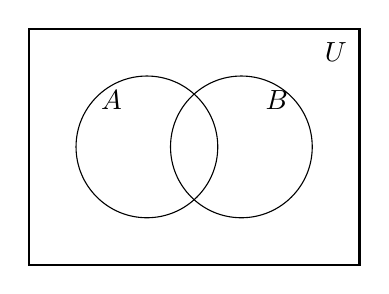
\begin{tikzpicture}[scale=.6]
    \draw[thick] (0,0) rectangle (7,5);
    \node at (6.5,4.5) {$U$};
    \draw (2.5,2.5) circle (1.5cm);
    \draw (4.5,2.5) circle (1.5cm);
    \node at (1.75,3.5) {$A$};
    \node at (5.25,3.5) {$B$};
\end{tikzpicture}
\end{exercise}

\begin{exercise}
Gegeven is dat $A$ de \textit{verzameling is van rode dingen}, en $B$ de \textit{verzameling van grote dingen}, en $x$ een variabele is over een universum $U$ (van objecten). Druk de volgende verzamelingen uit in $A$ en $B$ en de operatoren op verzamelingen:
\begin{enumerate}[label=\textit{\alph*.}]
    \item De verzameling $I$ van objecten die groot zijn als ze rood zijn.
    \item De verzameling $C$ van objecten die rood en groot zijn.
    \item De verzameling $E$ van objecten die rood zijn dan en slechts dan als ze groot zijn.
    \item De verzameling $D$ van objecten die rood of groot zijn.
\end{enumerate}
\end{exercise}

\begin{exercise}
Teken de bijbehorende Venn-diagrammen, en bewijs
\begin{enumerate}[label=\textit{\alph*.}]
    \item $A-(B-C)=A-(B-(A\cap C))$
    \item $(A-B)-C=A-(B\cup C)$
    \item $A-B=A-(A\cap B)$
    \item $A-B=(A\cup B)-B$
    \item $(A\Delta B)\cap C=(A\cap C)\Delta(B\cap C)$
\end{enumerate}
\end{exercise}

\begin{exercise}
Bestudeer de volgende uitspraken. Geef in geval van algemene juistheid een bewijs, geef anders een tegenvoorbeeld.
\begin{enumerate}[label=\textit{\alph*.}]
    \item $A-B=(A\cup C)-(B\cup C)$
    \item $A-B=(A\cap C)-(B\cap C)$
    \item $(A-B)\cup C=(A\cup C)-(B\cup C)$
    \item $(A-B)\cap C=(A\cap C)-(B\cap C)$
    \item $(A\Delta B)\cup C=(A\cup C)\Delta(B\cup C)$
\end{enumerate}
\end{exercise}

\begin{exercise}
Voor een verzameling $X$ met eindig veel elementen, geven we met $|X|$ het aantal elementen van $X$ aan. Alle in deze opgave voorkomende verzamelingen worden geacht eindig veel elementen te bezitten.
\begin{enumerate}[label=\textit{\alph*.}]
    \item Beredeneer dat $|A\cup B|=|A| + |B| - |A\cap B|$
    \item Gebruik het resultaat van a. om aan te tonen dat
    $$|(A\cup B\cup C)=|A|+|B|+|C|-|A\cap B|-|A\cap C|-|B\cap C|+|A\cap B\cap C|.$$
\end{enumerate}
\end{exercise}

\section{Machtsverzameling en cartesisch product}\label{sec:power}
Objecten hoeven geen ``ondeelbare'' dingen te zijn. Het komt zelfs vaak voor dat we hele verzamelingen als objecten wensen te beschouwen. Denk bijvoorbeeld aan een elftal, een regiment, een mierenkolonie.

Wellicht heb je op de middelbare school iets dergelijks ook gezien bij kansrekening, waar bijvoorbeeld gevraagd kan worden naar het aantal mogelijkheden waarop men uit een verzameling $V$ met $n$ objecten een groep kan maken. Dat is de vraag naar het aantal deelverzamelingen van $V$. Dat is het aantal \textit{elementen} van \emph{de verzameling bestaande uit de \textit{deelverzamelingen} van $V$}.

\newcommand{\power}{\ensuremath{\mathcal{P}}}

Deze verzameling noemen we de \textit{machtsverzameling} van $V$. In het Engels heet dit de \textit{power set}; we noteren hem dan ook met $\power(V)$:
$$\power(V) = \{A\;|\; A\subseteq V\}$$

We geven een voorbeeld. Zij $V=\{a,b,c\}$. Dan is 
$$\power(V)=\{\varnothing, \{a\},\{b\},\{c\},\{a,b\},\{a,c\},\{b,c\},\{a,b,c\} \}.$$

$\power(V)$ heeft in dit voorbeeld dus $8 (=2^3)$ elementen. In het algemeen bestaat $\power(V)$ uit $2^n$ elementen als $V$ uit $n$ elementen bestaat. Dit is als volgt in te zien. Een element van $\power(V)$ is een deelverzameling van $V$, en die ligt vast door voor elk element aan te geven of die wel of niet in de deelverzameling zit. Als $V$ bestaat uit $n$ elementen heb je hierbij dus $n$ keer een keuze uit twee mogelijkheden. In totaal levert dat $2^n$ mogelijkheden. Elke mogelijkheid correspondeert met precies \'e\'en deelverzameling, en elke deelverzameling kan zo worden verkregen, dus heeft $\power(V)$ precies $2^n$ elementen. Vanwege deze eigenschap wordt de machtsverzameling $\power(V)$ ook wel genoteerd als $2^V$; het woord \textit{machtsverzameling} is zo gekozen omdat hier sprake is van \textit{machtsverheffen}.

\begin{quote}
    Merk op dat we een onderscheid dienen te maken tussen het element $a$ en de verzameling $\{a\}$ die $a$ als enige element heeft.
    
    \noindent
    In het voorbeeld geldt wel $a\in \{a\}$ en $a\in V$ en $\{a\}\in\power(V)$ en $\{a\}\subseteq V$, maar niet $\{a\}\subseteq\power(V)$. Wel geldt $\{\{a\}\}\subseteq\power(V)$.
\end{quote}

Onder het \textit{cartesisch product} $A\times B$ van twee verzamelingen $A$ en $B$ verstaan we de verzameling van alle \textit{geordende paren} $(x,y)$ waarvoor $x\in A$ en $y\in B$.

Dat de paren geordende paren zijn, betekent dat $(x,y)$ en $(y,x)$ verschillend zijn als $x\not=y$.
$$A\times B=\{(x,y)\;|\; x\in A\wedge y\in B\}$$

Een voorbeeld: Zij
$$A=\{a,b,c,d\}\text{ en }B=\{a,d,f,e,g\}.$$
Dan is
$$\begin{array}{ccclllllc}
A\times B & = & \bigl\{ 
  & (a,a), & (a,d), & (a,f), & (a,e), & (a,g), & \\
  &&& (b,a), & (b,d), & (b,f), & (b,e), & (b,g), & \\
  &&& (c,a), & (c,d), & (c,f), & (c,e), & (c,g), & \\
  &&& (d,a), & (d,d), & (d,f), & (d,e), & (d,g), & \bigr\} \\
\end{array}$$

Als $A$ en $B$ eindige verzamelingen zijn met respectievelijk $n$ en $m$ elementen, heeft het cartesisch product $A\times B$ precies $n\times m$ elementen: voor elk geordend paar hebben we $n$ mogelijkheden om het eerste argument te kiezen en $m$ mogelijkheden om het tweede argument te kiezen. Dit verklaart waarom we dit een \textit{product} noemen. Het voorvoegsel is afgeleid van de wiskundige Ren\'e \textit{Descartes} (1596-1650), die de punten in het platte vlak opvatte als geordende paren van re\"ele getallen: de \textit{co\"ordinaten}.

Een reden dat we de begrippen machtsverzameling en cartesisch product als laatste hebben genoemd, is in de eerste plaats omdat ze abstracter (en wellicht onbekender) zijn dan de overige begrippen. Een andere reden is, dat deze constructies ons buiten een gegeven universum kunnen brengen. Men kan gemakkelijk zelf voorbeelden hiervan vinden.

\subsection{Opgaven}
\begin{exercise}\mbox{}
\begin{enumerate}[label=\textit{\alph*.}]
\item Gegeven is $A=\{1,2\}$ en $B=\{a,b\}$, bereken $A\times B$;
\item Gegeven is $A=\{1,2\}$ en $B=\{a,b\}$, bereken $B\times A$;
\item Gegeven is $Z=\{0,1,7,8\}$ en $Y=\{0,1\}$, bereken $Z\times Y$;
\item Gegeven is $A=\{f,k\}$ en $B=\varnothing$, bereken $A\times B$;
\item Gegeven is $V=\{f,t\}$ en $S=\{c,d,u\}$, bereken $V\times S$.
\end{enumerate}
\end{exercise}

\begin{exercise} Bereken:
\begin{enumerate}[label=\textit{\alph*.}]
\item $\power(A)$ als $A = \{1,3,4,5\}$;
\item $\power(B)$ als $B=\{\varnothing, 1,3\}$;
\item $\power(C)$ als $C=\{1,\{2,3\},\{\{4,5\}\}\}$.
\end{enumerate}
\end{exercise}

\begin{exercise}\mbox{}
\begin{enumerate}[label=\textit{\alph*.}]
\item Als $A$ een verzameling is en $|A|=5$, wat is dan $|\power(A)|$?
\item Als $A$ een verzameling is en $|A|=5$, wat is dan $|A\times A|$?
\item Als $A=\{12,14,5,1\}$, wat is dan $|(A\times A)\cup A|$?
\end{enumerate}
\end{exercise}

\begin{exercise} Bepaal voor elk van de volgenden of deze een power set zijn van een of andere verzameling $A$ (en definieer wat $A$ dan precies is). Neem aan dat $a$ en $b$ verschillende elementen zijn.
\begin{enumerate}[label=\textit{\alph*.}]
\item $\varnothing$;
\item $\{\varnothing,\{a\}\}$;
\item $\{\varnothing,\{a\},\{\varnothing,\{a\}\}\}$;
\item $\{\varnothing,\{a\},\{b\},\{a,b\}\}$.
\end{enumerate}
\end{exercise}

\begin{exercise}[Bonus]\mbox{}\\
Vindt twee verzamelingen $A$ en $B$ zodanig dat $A\in B$ \'en $A\subseteq B$.
\end{exercise}

\section{Functies}\label{sec:functies}
Wanneer we voor twee verzamelingen $A$ en $B$ bij elk element van $A$ precies \'e\'en element van $B$ vastleggen, dan hebben we een \textit{afbeelding} van $A$ naar $B$ gedefinieerd. In plaats van afbeelding zegt men ook wel \textit{functie}. In het Engels heet een afbeelding een \textit{map} of \textit{function}.

Door middel van een afbeelding van $A$ naar $B$ wijst elk element van $A$ dus een element van $B$ aan. Een element van $B$ kan vaker aangewezen worden. Een element van $A$ kan niet meer dan \'e\'en element van $B$ aanwijzen. Wij zullen ons meestal bedienen van deze terminologie van aanwijzen. Dit komt ook overeen met de veelgebruikte manier om een afbeelding van $A$ naar $B$ te visualiseren door middel van een tekening waarin vanuit elk punt van een getekende verzameling $A$ een pijl vertrekt die aankomt in een van de punten van de getekende verzameling $B$.
\begin{center}
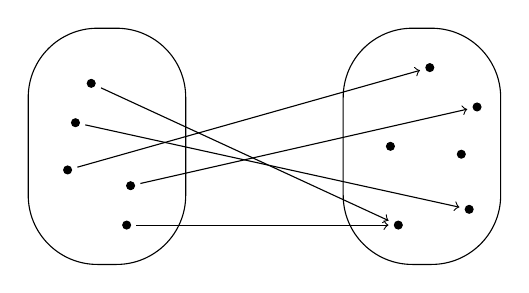
\begin{tikzpicture}
\draw[rounded corners=25pt] (0,0) rectangle (2,3);
\draw[rounded corners=25pt] (4,0) rectangle (6,3);
\draw[fill] (1.25, .5) circle (.05cm) node (a1) {};
\draw[fill] (1.3, 1) circle (.05cm) node (a2) {};
\draw[fill] (0.5, 1.2) circle (.05cm) node (a3) {};
\draw[fill] (0.6, 1.8) circle (.05cm) node (a4) {};
\draw[fill] (0.8, 2.3) circle (.05cm) node (a5) {};
\draw[fill] (4.7, .5) circle (.05cm) node (b1) {};
\draw[fill] (5.6, .7) circle (.05cm) node (b2) {};
\draw[fill] (4.6, 1.5) circle (.05cm) node (b3) {};
\draw[fill] (5.5, 1.4) circle (.05cm) node (b4) {};
\draw[fill] (5.7, 2.0) circle (.05cm) node (b5) {};
\draw[fill] (5.1, 2.5) circle (.05cm) node (b6) {};

\draw[->] (a1) -- (b1);
\draw[->] (a2) -- (b5);
\draw[->] (a3) -- (b6);
\draw[->] (a4) -- (b2);
\draw[->] (a5) -- (b1);
\end{tikzpicture}
\end{center}

Zo'n plaatje heet ook wel een \textit{pijlendiagram}.

Een afbeelding bestaat dus uit een drietal: een verzameling $A$, een verzameling $B$, en een beschrijving die aangeeft hoe de aanwijzing van elementen van $B$ door de elementen van $A$ er uitziet.

Korten we die beschrijving af door een letter, bijvoorbeeld $f$, dan is de afbeelding dus het drietal $(A, B, f)$.
$$A\text{ heet het \textit{domein} van }f\text{ (Engels: \textit{domain}),}$$
$$B\text{ heet het \textit{codomein} van }f\text{ (Engels: \textit{codomain}).}$$

Een suggestieve en zeer vaak gebruikte notatie is
$$f: A\rightarrow B.$$
Alhoewel de pijl hier verward zou kunnen worden met de logische pijl, staat de context er vrijwel altijd borg voor dat dit niet gebeurt. De combinatie $A\rightarrow B$ van domein en codomein heet wel het \textit{type} van de afbeelding $f$. Voor het codomein zul je soms ook de term \textit{bereik} (Engels: \textit{range}) tegenkomen; deze term wordt echter ook gebruikt voor een ander, gerelateerd, concept dat verderop besproken wordt, en zal in deze tekst verder vermeden worden.

Is $x$ een element van $A$, dan duidt $f(x)$ het \textit{beeld} van $x$ aan (Engels: \textit{image}), het element van $B$ dat door $x$ wordt aangewezen. Het element $x$ heeft dan wel het \textit{argument} van de afbeelding.

Twee afbeeldingen $f:A\rightarrow B$ en $g:C\rightarrow D$ zijn aan elkaar \textit{gelijk} (en dus dezelfde afbeelding), precies dan als aan drie voorwaarden voldaan is:
\begin{enumerate}
    \item $A = C$;
    \item $B = D$;
    \item voor alle $x\in A$ geldt dat $f(x) = g(x)$.
\end{enumerate}
\begin{example}
Enkele voorbeelden van afbeeldingen zijn:
\begin{itemize}
    \item $A=\mathbb{R}, B=\mathbb{R},$ voor alle $x\in\mathbb{R}$ is $f(x)=\text{sin}(x)$;
    \item $A=\{1, 2, 3\}, B=\{a, b, c, d\}, f(1)= b, f(2) = d, f(3) = b$;
    \item $A=\mathbb{N}, B=\{2,3,5,6\},$ voor alle $n\in\mathbb{N}$ is $f(n)=5$.
\end{itemize}
In het vervolg zullen we het tweede voorbeeld nog een aantal keren aanhalen. Enkele gevallen waarin we niet met een afbeelding van doen hebben, zijn:
\begin{itemize}
    \item $A=\mathbb{R}, B=\mathbb{R}, f(x)=\text{ln}(x)$,\\ want $\text{ln}(x)$ is niet voor elke $x\in\mathbb{R}$ gedefinieerd.
    \item $A=\mathbb{N}, B=\mathbb{Q}, f(x)=\sqrt{x}$,\\ want $\sqrt{2}\not\in\mathbb{Q}$.
\end{itemize}\label{vb:func}
\end{example}

Bij een afbeelding $f:A\rightarrow B$ en een deelverzameling $X$ van $A$ kunnen we kijken naar de deelverzameling van $B$ bestaande uit de beelden van alle elementen van $X$. Deze deelverzameling van $B$ heet het \textit{beeld} (Engels: \textit{image}) van $X$, en wordt aangeduid met $f(X)$. Ook het beeld wordt vaak aangeduid met de term \textit{bereik}; het kan dus per tekst verschillen of met deze term het grotere codomein bedoeld wordt, of de deelverzameling van het beeld. In deze tekst gebruiken we de ondubbelzinnige termen \textit{codomein} en \textit{bereik}, en raden jullie aan hetzelfde te doen.
$$f(X) = \{y\in B\;|\;\text{er is een } x\in X(y=f(x))\}$$
Merk op dat zowel de notatie als de terminologie hiervan overeenkomt met het beeld van een element. Uit de context moet dus worden opgemaakt om welk van de twee begrippen het gaat: als $x$ een element is van $A$ dan is $f(x)$ het bijbehorende element van $B$; als $x$ een deelverzameling is van $A$ dan is $f(x)$ de deelverzameling van $B$ bestaande uit bij die deelverzameling horende elementen van $B$.

In het voorbeeld van \ref{vb:func} hebben we onder andere
$$f(\{1\})=\{b\}, f(\{1,2\})=\{b,d\}, f(\{1,3\})=\{b\},f(A)=\{b,d\}$$

De verzameling $f(A)$ wordt wel het \textit{beeld} van $f$ genoemd. Ook kunnen we bij een deelverzameling $Y$ van $B$ vragen naar de deelverzameling van $A$ bestaande uit alle $x$ waarvoor $f(x)\in Y$.

In bijlage \ref{app:functies} wordt nog meer eigenschappen en bijzonderheden van functies besproken.

\subsection{Opgaven}

\begin{exercise}
  Ga na of de volgende relaties tevens functies zijn:\mbox{}\\
  \begin{enumerate}[label=\textbf{\alph*.}]
    \item de relatie kind-ouder;
    \item de relatie tussen een persoon en de verzameling van diens ouders;
    \item de relatie tussen een persoon en diens vaste partner;
    \item de relatie tussen een geheel getal en het getal met $1$ opgehoogd;
    \item de relatie tussen een getal en het kwadraat van dat getal;
    \item de relatie tussen een getal en de vierkantswortel van dat getal.
  \end{enumerate}
\end{exercise}

\begin{exercise}\mbox{}\\
  \begin{enumerate}[label=\textbf{\alph*.}]
    \item Gegeven zijn de verzamelingen $K = \{ \text{Wilhelmina}, \text{Juliana}, \text{Beatrix},$\\ $\text{Willem-Alexander}, \text{Amalia} \}$ en de volgende pijlen:
  \begin{align*}
    \text{Wilhelmina} &\longrightarrow \text{Juliana}\\
    \text{Juliana} &\longrightarrow \text{Beatrix}\\
    \text{Beatrix} &\longrightarrow \text{Willem-Alexander}\\
    \text{Willem-Alexander} &\longrightarrow \text{Amalia}
  \end{align*} Hebben we hier met een geldige functie $K \to K$ te maken?\\ Zo nee, wat zouden we moeten aanpassen om wel een geldige functie te defini\"{e}ren?\\

  \item Gegeven zijn de verzameling $H = \{ \text{steen}, \text{papier}, \text{schaar} \}$ en de volgende pijlen:
  \begin{align*}
    \text{steen} &\longrightarrow \text{schaar}\\
    \text{papier} &\longrightarrow \text{steen}\\
    \text{schaar} &\longrightarrow \text{papier}
  \end{align*} Hebben we hier met een geldige functie $H \to H$ te maken?\\ Zo nee, wat zouden we moeten aanpassen om wel een geldige functie te defini\"{e}ren?
  \end{enumerate}
\end{exercise}

\begin{exercise}\mbox{}\\
  \begin{enumerate}[label=\textbf{\alph*.}]
    \item Gegeven zijn de verzameling $S = \{ \text{winter}, \text{lente}, \text{zomer}, \text{herfst} \}$ en de afbeelding $v : S \to S$:
  \begin{equation*}
  \begin{aligned}
    \text{winter} &\longrightarrow \text{lente}\quad\quad\quad &
    \text{zomer} &\longrightarrow \text{herfst}\\
    \text{lente} &\longrightarrow \text{zomer}&
    \text{herfst} &\longrightarrow \text{winter}
  \end{aligned}
  \end{equation*}
  \begin{enumerate}[label=\textbf{\alph*.}]
      \item Wat is de waarde van $v(\text{zomer})$?
      \item Wat is het type\footnote{Tot welke verzameling behoort deze waarde?} van $v(\text{zomer})$?
      \item Heeft het zin om over de waarde $v(v(\text{winter}))$ te redeneren?\\ Zo ja: wat is deze waarde; zo nee: waarom niet?\\
  \end{enumerate}

  \item Gegeven zijn de verzamelingen $D_{1} = \{ \text{David}, \text{Matt}, \text{Peter} \}$, $D_{2} = \{ \text{Matt}, \text{Peter}, \text{Jodie} \}$ en de afbeelding $r : D_{1} \to D_{2}$:
  \begin{equation*}
  \begin{aligned}
    \text{David} &\longrightarrow \text{Matt}\quad\quad
    \text{Peter} &\longrightarrow \text{Jodie}\\
    \text{Matt} &\longrightarrow \text{Peter}
  \end{aligned}
  \end{equation*}
  \begin{enumerate}[label=\textbf{\alph*.}]
      \item Wat is de waarde van $r(\text{David})$?
      \item Wat is het type van $r(\text{David})$?
      \item Heeft het zin om voor $x \in D_{1}$ over de waarde $r(r(x))$ te redeneren?\\ Beargumenteer je antwoord.
  \end{enumerate}
  \end{enumerate}
\end{exercise}

\begin{exercise}\mbox{}\\
  \begin{enumerate}[label=\textbf{\alph*.}]
    \item Gegeven is de functie $f(x) = 2x + 1$. We kunnen hier verschillende keuzes voor het domein maken; het codomein zal hiervan afhankelijk zijn.
      \begin{enumerate}
        \item Wat is het codomein als het domein $\mathbb{N}$ is?
        \item Wat is het beeld\footnote{Hint: voor deze verzameling hebben we geen symbool zoals $\mathbb{N}$, maar toch is deze eenduidig te beschrijven als deelverzameling van het codomein dat je al gevonden hebt.} als het domein $\mathbb{N}$ is?
        \item Wat is het codomein als het domein $\mathbb{R}$ is?
      \end{enumerate}

    \item Gegeven is de functie $f(x) = 3^{x} - 2$. We kunnen hier verschillende keuzes voor het domein maken; het codomein zal hiervan afhankelijk zijn.
      \begin{enumerate}
        \item Wat is het codomein als het domein $\mathbb{N}$ is?
        \item Wat is het codomein als het domein $\mathbb{N}_{1}$ is, waarbij $\mathbb{N}_{1} = \mathbb{N} - \{0\}$, oftewel de verzameling van alle positieve gehele getallen?
        \item Wat is het codomein als het domein $\mathbb{Z}$ is?
        \item Wat is het codomein als het domein $\mathbb{Q}$ is?
      \end{enumerate}


  \end{enumerate}
\end{exercise}

\chapter{Predikaatlogica}\label{ch:predicaten}
In hoofdstuk \ref{ch:proposities} hebben we de propositielogica ge\"introduceerd als een formalisme waarmee redeneringen kunnen worden beschreven. Hierbij konden redeneringen worden geanalyseerd tot op het niveau van enkelvoudige beweringen. Een groot aantal redeneringen, ook wiskundige, kan niet met behulp van de propositielogica worden geanalyseerd. Immers, de interne structuur van de enkelvoudige beweringen wordt buiten beschouwing gelaten. Als eerste voorbeeld komen we terug op de postbode uit het eerste hoofdstuk.

De redenering begon als volgt: Stel dat de bewering `er is een adres waarop vier of meer stukken zijn afgeleverd' niet waar is, dan geldt: `voor alle adressen zijn er hoogstens drie stukken afgeleverd'. Voor het redeneren met \textit{vier of meer} en \textit{hoogstens drie} kunnen we nog wel af met gewone rekenregels, maar voor het redeneren met \textit{er is een} en \textit{voor alle} hebben we nog niets.

De taal van de propositielogica is voor veel toepassingen te arm. Dat bleek al in de Klassieke Oudheid, waar logici allerlei redeneerpatronen vonden die te maken hebben met de manier waarop wij in natuurlijke taal objecten beschrijven, en hun eigenschappen en relaties. Dan gaan andere uitdrukkingen een sleutelrol spelen dan connectieven als `niet' of `en', met name de \textit{kwantoren} `alle' en `sommige'. Maar net als in hoofdstuk \ref{ch:proposities} komt deze noodzaak tot uitbreiding het scherpst naar voren als we kijken naar wiskundig redeneren, en dus beginnen we ook weer daar om te zien wat voor rijker logisch systeem we nu nodig hebben.

In de wiskunde doen we graag algemene uitspraken over objecten uit een oneindige verzameling en van de logica verlangen we dat we deze uitspraken heel precies kunnen weergeven, en er de juiste gevolgen uit af kunnen leiden. De propositielogica is hiervoor niet altijd geschikt. Bijvoorbeeld de uitspraak:
\begin{quote}
    `elk even getal groter dan 2 is de som van twee priemgetallen' (het zogenaamde vermoeden van Goldbach)
\end{quote}
kan niet goed worden weergegeven in propositielogica.

Wat bedoelen we hier met `goed weergegeven'? Om dat te zien, doen we een klein `gedachten-experiment': stel dat we wel een geschikte formule uit de propositielogica hadden, hoe zou die er dan uit moeten zien? Aangezien er in de uitspraak geen voegwoorden te onderscheiden zijn, zouden we de uitspraak als een propositieletter moeten weergeven, zeg door `$p$'.

Beschouw nu de uitspraak:
\begin{quote}
    `2018 is de som van twee priemgetallen'
\end{quote}
Dit volgt uit het vermoeden van Goldbach, dat wil zeggen, als het vermoeden van Goldbach juist is, dan is 2018 inderdaad te schrijven als de som van twee priemgetallen. Maar `2018 is de som van twee priemgetallen' is een andere uitspraak dan het vermoeden van Goldbach. Er zit niets anders op dan hiervoor een andere propositieletter te kiezen, zeg $q$. Maar dan doet zich het probleem voor dat $p\not\vdash q$, dat wil zeggen, $q$ is geen logisch gevolg van $p$, want $p$ kan waar zijn terwijl $q$ onwaar is. Het antwoord op de vraag of $q$ een logisch gevolg is van $p$, staat namelijk los van de relatie tussen de uitspraken waar $p$ en $q$ vertalingen van zouden moeten zijn: de symbolen $p$ en $q$ zijn bij wijze van spreken `losgeweekt' van de getaltheoretische context.

De conclusie is dus dat $p$ geen goede weergave is van het vermoeden van Goldbach, en eigenlijk lag dat ook wel voor de had: de interne structuur van de uitspraak is niet in de formule $p$ terug te vinden.

Een andere poging om `Goldbach' in propositielogica weer te geven is: laat $p_i$ staan voor `$i$ is de som van twee priemgetallen'. Dan zouden we het vermoeden van Goldbach door een oneindig lange conjunctie kunnen weergeven: $p_4\wedge p_6\wedge p_8\wedge p_{10}\wedge\ldots$. Dit zou inderdaad $p_{2018}$ tot gevolg hebben. Maar een oneindig lange conjuctie is geen `formule' volgens definitie \ref{def:prop} van de taal van de propositielogica. We kunnen namelijk eenvoudig inzien dat iedere formule een eindig aantal symbolen bevat. Lange conjunctie mag, maar oneindige niet. Dus ook deze weg loopt in eerste instantie dood.

Het systeem van de predikaatlogica, waarmee we in de komende hoofdstukken kennismaken, heeft een veel grotere uitdrukkingskracht dan de propositielogica, waar ze een verfijning en uitbreiding van is. Het vermoeden van Goldbach en zijn gevolgen kunnen we in predikaatlogica w\'el goed weergeven. We maken eerst kennis met de taal van de predikaatlogica en met een methode om situaties aan te geven waarin een predikaatlogische formule waar is. In het volgende hoofdstuk kijken we naar het interpreteren van predikaatlogische formules en naar predikaatlogisch gevolg.

\section{Bouwstenen van de predikaatlogica}
In de propositielogica konden we een eenvoudige uitspraak als `Judith schaakt' alleen maar weergeven door een propositieletter. In de predikaatlogica kunnen we de interne structuur van zulke uitspraken zichtbaar maken.

\begin{example}\label{vb:pred:1}
`Judith schaakt' wordt in predikaatlogica weergegeven als $S(j)$. Hierin staat $S$ voor de eigenschap `schaken' die toekomt aan het object `Judith', dat met $j$ is aangeduid (`object' wordt hier in algemene zin gebruikt: daaronder vallen ook menselijke individuen). De eigenschap staat voorop, het object er tussen haakjes achter.
\end{example}

De predikaatlogica bevat uitdrukkingen die \textit{predikaten} (dat wil zeggen: eigenschappen van objecten en relaties tussen objecten) aangeven: dat noemen we \textit{predikaatsymbolen}. Daarnaast zien we namen voor objecten: de \textit{constanten}. In het voorbeeld is $S$ dus een predikaatsymbool en $j$ een constante. Voor predikaatsymbolen gebruiken we hoofdletters $A,\ldots,Z$ of speciale symbolen zoals `='. Voor constanten worden kleine letters $a,\ldots, t$ en ook wel getallen gebruikt. De letters $u,\ldots,z$ gebruiken we als variabelen.

We kiezen over het algemeen letters die makkelijk te onthouden zijn, bijvoorbeeld de beginletter van het met het predikaatsymbool overeenkomstige woord. Maar logisch gezien is er geen enkel verband tussen een letter en de daarmee bedoelde eigenschap (en eigenlijk is dit evenmin zo als we getallen gebruiken als constante symbolen), dus dit verband moeten we expliciet aangeven door middel van een zogeheten vertaalsleutel.

\begin{example}\label{vb:pred:2}
De uitspraken:
\begin{itemize}
    \item Marie is wiskundige.
    \item 5 is een priemgetal.
\end{itemize}
kunnen in predikaatlogica worden weergegeven door respectievelijk:
\begin{itemize}
    \item $m:$ Marie
    \item $5:$ het getal vijf
    \item $W:$ is wiskundige
    \item $P:$ is een priemgetal
\end{itemize}
In het vervolg laten we het vermelden van de vertaalsleutel vaak achterwege wanneer deze erg voor de hand ligt. De predikaatsymbolen in dit voorbeeld zijn dus $W$ en $P$ en de constanten zijn $m$ en $5$. Ook zullen we meestal zeggen dat we de constante $5$ vertalen als het getal $5$, als `zichzelf', als het ware; ook al is daar formeel een verschil tussen.
\end{example}

Ook relaties, zowel in wiskundige als in andere zin, kunnen we logisch aanduiden met predikaatsymbolen. Het volgende voorbeeld laat zien dat we dan ook weer moeiteloos van wiskundige taal op natuurlijke taal kunnen overstappen.

\begin{example}\label{vb:pred:3}
De uitspraken:
\begin{itemize}
    \item Jan houdt van Marie.
    \item 5 is groter dan 3.
\end{itemize}
kunnen in predikaatlogica worden vertaald als:
\begin{itemize}
    \item $H(j, m)$
    \item $G(5, 3)$
\end{itemize}
Merk op dat ook hier de predikaatsymbolen voorop staan, gevolgd door de objecten tussen haakjes en door komma's gescheiden. De weergave $G(5,3)$ wijkt echter wel erg af van de wiskundige praktijk. In plaats van $G$ gebruiken we dan altijd het symbool `$>$'; en dat wordt gewoon tussen de constanten in geschreven, zodat we de volgende bekende notatie gebruiken:
\begin{itemize}
    \item $5>3$
\end{itemize}
\end{example}

Ook andere gangbare relaties zoals gelijkheid `$=$', kleiner dan `$<$' en groter dan of gelijk aan `$\geq$', worden door de bekende symbolen weergeven en tussen de constanten geschreven in plaats van ervoor.

Predikaatsymbolen zoals $P$ en $W$ in voorbeeld \ref{vb:pred:2} worden door slechts \'e\'en constante gevolgd: zulke predikaatsymbolen worden \textit{\'e\'enplaatsig} genoemd. De predikaatsymbolen in voorbeeld \ref{vb:pred:3} hebben twee constanten bij zich: we noemen deze \textit{tweeplaatsig}.

Eigenschappen worden dus in de regel door 1-plaatsige predikaatsymbolen weergeven, binaire relaties door 2-plaatsige. Hier houdt het niet mee op: er zijn ook 3-plaatsige, 4-plaatsige en in het algemeen $n$-plaatsige predikaatsymbolen.

\begin{example}\label{vb:pred:4}
De uitspraken:
\begin{itemize}
    \item $1/2$ ligt tussen 0 en 1.
    \item Marie geeft Jan `De Aanslag'.
    \item punt $D$ heeft dezelfde afstand tot $P$, $Q$ en $R$.
\end{itemize}
kunnen in predikaatlogica worden weergegeven door:
\begin{itemize}
    \item $T(1/2,0,1)$
    \item $G(m,j,a)$
    \item $A(d,p,q,r)$
\end{itemize}
\end{example}

Naast constanten, die elk een bepaald vast object aanduiden, willen we ook graag over symbolen beschikken die \textit{verschillende} objecten kunnen aanduiden.
\begin{example}
De uitspraken:
\begin{itemize}
    \item $x$ is groter dan 3.
    \item Marie houdt van hem.
\end{itemize}
kunnen worden weergegeven door:
\begin{itemize}
    \item $x>3$
    \item $H(m,x)$
\end{itemize}
In beide gevallen hangt het van de situatie af wat `$x$' (of `hem') is. Bijvoorbeeld, als $x=5$, dan krijgen we $5>3$, maar als $x=10$, dan krijgen we $10>3$.
\end{example}

Net als in de wiskunde noemen we $x$ een variabele. De letters $y$ en $z$, en soms ook $u$ en $v$, worden eveneens gebruikt als variabele, eventueel vergezeld van een accent ($x'$) of een index ($x_0$). Zo'n `variabele constante' $x$ (een naamgeving waar we niet omheen kunnen, ook al lijkt het tegenstrijdig) lijkt dus wat op de propositionele formulevariabelen zoals $\varphi$ en $\psi$. Er is echter een belangrijk verschil; variabele constanten zoals $x$ gaan echt deel uitmaken van de predikaatlogische taal. Terwijl formulevariabelen niet meer dan `plaatsvervangende' formules zijn, die we later nog kunnen concretiseren om er echte formules van te maken.

In de predikaatlogica hebben we geen propositieletters. Het is wel van belang dat we beschikken over haakjes en connectieven. Met behulp van de connectieven $\neg,\wedge,\vee,\rightarrow$ en $\leftrightarrow$ kunnen we nu ook ingewikkeldere uitspraken weergeven in predikaatlogica. Dit zou je ook `vertalen' kunnen noemen.

\begin{example}
De uitspraken:
\begin{itemize}
    \item Jan houdt van Marie, maar Marie niet van Jan.
    \item $x$ is groter dan 0 of $y$ is kleiner dan 1.
    \item als $x$ groter is dan 3 en een priemgetal is, dan is $x$ oneven.
\end{itemize}
kunnen vertaald worden als:
\begin{itemize}
    \item $H(j,m)\wedge\neg H(m,j)$
    \item $x>0\vee y<1$
    \item $(x>3\wedge P(x))\rightarrow O(x)$
\end{itemize}
De laatste uitspraak gaat dus over een specifieke, zij het nog onbekende waarde voor $x$. Ze wordt ook vaak algemener opgevat, namelijk als: `\textit{voor elke $x$ geldt}, dat als $x$ groter is dan 3 en een priemgetal, dan is $x$ oneven'. Dat bedoelen we hier niet, maar dat kunnen we wel in predikaatlogica uitdrukken, en daar vervolgende we nu mee.
\end{example}

Algemene feiten van het soort `voor elke $x$ geldt dat als $x$ een priemgetal groter dan 3 is, dan is $x$ oneven' zijn heel precies uit te drukken in predikaatlogica. De formule $(x>3\wedge P(x))\rightarrow O(x)$ voldoet echter niet, want daarin heeft $x$ nog steeds een specifieke (maar een `verzwegen') waarde. Wat we expliciet moeten aangeven, is dat hier alle mogelijke waarden voor $x$ op het oog hebben. Dit doen we door de zogenaamde kwantor $\forall$ (spreek uit: `voor elke \ldots' of `voor alle \ldots') en de betreffende variabele voor de formule te zetten, resulterend in:
$$\forall x(x>3\wedge P(x))\rightarrow O(x)$$
Het symbool $\forall$ wordt (al dan niet in combinatie met variabele) de \textit{universele kwantor} of \textit{al-kwantor} genoemd.

\begin{aside}[Kwantoren (ook wel quantoren)]\mbox{}\\
Kwantificatie is een begrip uit de wiskunde en taalkunde om uitspraken te doen over meerdere elementen van een \textit{domain of discourse} (een universum waarover uitspraken worden gedaan). In de natuurlijke taal kennen we meerdere kwantoren, zoals \textit{voor alle}, \textit{voor sommige}, \textit{vele}, \textit{enige}, \textit{geen enkele}.

Door zijn voorkomen in natuurlijke taal, zijn kwantoren al lang in gebruik (hoewel de precieze aard van de kwantoren pas later werden gedefinieerd). Al in de logica van Aristoteles (390 B.C.), werd veelvuldig gebruik gemaakt van kwantoren. De concepten \textit{voor alle}, \textit{voor sommige}, \textit{geen enkele}, werden in de formele redeneringen van dit systeem gebruikt. Het bekendste voorbeeld is het klassieke syllogisme (bedacht door Aristoteles): `Alle mensen zijn sterfelijk, Socrates is een mens, dus Socrates is sterfelijk'.

Pas in de 19e eeuw werden kwantoren formeel in de logica ingevoerd, eerst door \citet{demorgan}. Pas later, in het werk van \citet{frege:begriffschrift} en \citet{russel:principia:1,russel:principia:2,russel:principia:3}, werden kwantoren gecombineerd met het predikaatlogische systeem.

Het principe van variabele binding door middel van kwantoren komt ook in andere formalismen voor, denk bijvoorbeeld maar aan het som $\sum^k_i x_i$, het product $\prod^k_i x_i$ en integralen $\int_{a}^{b} x^2 dx$ uit de wiskunde. Vergelijkbaar met deze wiskundige kwantoren zijn de logische kwantoren in principe ook een afkorting voor een langere formule. De \textit{universele kwantor} is een afkorting voor een langere (mogelijk oneindige) formule: $\forall x\;P(x) \Leftrightarrow P(x_0)\wedge P(x_1)\wedge P(x_2)\wedge\ldots\wedge P(_n)$ (voor alle $x_i$ uit het domein). De \textit{existenti\"ele kwantor} vertaalt naar een (oneindige) disjunctie: $\exists x\;P(x)\Leftrightarrow P(x_0)\vee P(x_1)\vee P(x_2)\vee\ldots\vee P(x_n)$ (wederom, voor alle $x_i$ in het domein).
\end{aside}

\begin{example}
Om de uitspraak `Alle wiskundigen schaken' in predikaatlogica weer te geven, herschrijven we de uitspraak in vormen die het mogelijk maken de tot nu toe ge\"introduceerde begrippen te gebruiken. We gaan daarbij stukje bij beetje te werk. De stukjes die aangepakt worden, zijn steeds onderstreept.

\noindent
\underline{Alle} wiskundigen schaken.\\
$\forall x$(\underline{als} $x$ wiskundige is, \underline{dan} schaakt $x$ )\\
$\forall x (x$ \underline{is wiskundige}$\rightarrow x$ \underline{schaakt})\\
$\forall x(W(x)\rightarrow S(x))$
\end{example}

Ook voor meer ingewikkelde gevallen kunnen we deze methode gebruiken, maar nog belangrijker is dat je een patroon in de predikaatlogische formules ontdekt. We vervolgen met nog een ander voorbeeld.
\begin{example}
De uitspraken:
\begin{itemize}
    \item Alle natuurlijke getallen zijn groter dan of gelijk aan 0.
    \item Elk natuurlijk getal is groter dan elk negatief geheel getal.
\end{itemize}
kunnen worden weergegeven door de volgende formules:
\begin{itemize}
    \item $\forall x(N(x)\rightarrow x\geq 0)$
    \item $\forall x(N(x)\rightarrow\forall y((Z(y)\wedge y< 0)\rightarrow x> y))$
\end{itemize}
We zien dat de universele kwantor hier in beide gevallen met een implicatie optreedt. Voor `$x$ is een natuurlijk getal' kunnen we natuurlijk ook $x\in\mathbb{N}$ schrijven, en voor `$x$ is een geheel getal': $x\in\mathbb{Z}$. Die meer vertrouwde schrijfwijzen komen op hetzelfde neer.
\end{example}

Het patroon $\forall x(\ldots\rightarrow\ldots)$ komt ontzettend vaak voor. Dat is geen toeval, want vaak willen we iets uitdrukken als `voor alle dingen die aan een bepaalde eis voldoen, geldt dat \ldots'. Die eis komt dan links van het implicatieteken te staan. Dit is geen wet van Meden en Perzen: formules als $\forall x W(x)$ en $\forall x\forall y R(x,y)$ zijn zonder meer correct en kunnen heel zinvolle uitspraken zijn.

Een ander type uitspraak is van de vorm `Er is een \ldots'. De predikaatlogica is daarom uitgerust met een tweede kwantor, de \textit{existenti\"ele kwantor}. Daarbij moet $\exists x$ (spreek uit: `er is een $x$') worden opgevat als `voor minstens \'e\'en $x$'.

\begin{example}\label{vb:pred:vader}
De uitspraken:
\begin{itemize}
    \item Jan houdt van iemand.
    \item Marie is groter dan haar vaders vader.
    \item 2 is het enige even priemgetal.
\end{itemize}
kunnen worden weergegeven door de volgende formules:
\begin{itemize}
    \item $\exists x\; H(j,x)$
    \item $\exists x(V(x,m)\wedge\exists y(V(y,x)\wedge m>y))$
    \item $E(2)\wedge P(2)\wedge\neg\exists x(x\not= 2\wedge E(x)\wedge P(x))$
\end{itemize}
Informeel gesproken is bij de tweede uitspraak $x$ Maries vader en $y$ Maries opa van vaderskant. Wat we hier niet hebben uitgedrukt, is dat Marie maar \'e\'en vader heeft, enzovoorts. We kunnen dit wel uitdrukken, namelijk als in de derde formule, maar het wordt dan een tamelijk ingewikkelde formules. Bij de derde uitspraak moeten we bedenken dat deze neerkomt op `2 is een even priemgetal en er zijn geen andere even priemgetallen'. Net als in de propositielogica geldt hier dat er equivalente formules gegeven kunnen worden; zo kunnen we voor de laatste formule ook de vertaling $ \forall x((E(x)\wedge P(x))\leftrightarrow x=2$ geven.
\end{example}

Ook in dit voorbeeld zien we een patroon opduiken: de existenti\"ele kwantor gaat vaak vergezeld van een conjunctie. En hoewel ook hier geldt dat $\exists$ best zonder $\wedge$ kan optreden (zoals in $\exists x\; V(x)$), zien we inderdaad het patroon $\exists x(\ldots\wedge\ldots)$ heel regelmatig terugkeren.

Net zoals bepaalde uitspraken vaak universeel worden opgevat, zien we dat andere zoals `Marie houdt van hem' door sommigen eerder existentieel opgevat, dat wil zeggen: gelezen worden als `er is iemand waar Marie van houdt'. Ook `$x$ is groter dan 3 en $y$ is kleiner dan 4' zal soms existentieel worden gelezen. Toch is het duidelijk dat we dit niet altijd willen: denk bijvoorbeeld aan een probleem dat we aan het oplossen zijn waarbij we de te zoeken grootheden $x$ en $y$ genoemd hebben. We willen echter wel degelijk de waarden van $x$ en $y$ achterhalen, en niet alleen maar beweren dat zulke waarden bestaan.

Zonder overdrijving kunnen we stellen dat het vooral de kwantoren zijn die de predikaatlogica haar uitdrukkingskracht verlenen. We laten de kracht van de predikaatlogica nog even zien aan de hand van het vermoeden van Goldbach (zie ook het begin van dit hoofdstuk).

\begin{example}\label{vb:pred:goldbach:formeel}
Het vermoeden van Goldbach kunnen we weergeven door:
$$\forall x((E(x)\wedge x\geq 2)\rightarrow\exists y\exists z(P(y)\wedge P(z)\wedge S(x,y,z)))$$
We hebben hier van een nieuw 3-plaatsig predikaatsymbool $S$ gebruik gemaakt, waarbij $S(x,y,z)$ staat voor `$x$ is de som van $y$ en $z$'.
\end{example}
Dit voorbeeld illustreert dat we in predikaatlogica inderdaad aardig wat wiskunde kunnen weergeven. Goldbach's vermoeden is een openstaand probleem uit de getaltheorie, en we zouden kunnen denken dat we misschien met logica kunnen uitzoeken of het vermoeden waar is of niet. Wie dat denkt, komt bedrogen uit. De formule geeft weliswaar de globale logische structuur van het vermoeden weer, maar de predikaatsymbolen die erin voorkomen, hebben nog geen specifieke eigenschappen: voor de logica zou $E$ net zo goed kunnen staan voor `een getal dat met het cijfer 1 begint'.

\begin{example}
De uitspraak `Ze kwam binnen en deed het licht uit' kan niet goed door propositielogica worden weergegeven. Een conjunctie $p\wedge q$ doet geen recht aan de tijdsordening. Het betekent namelijk iets anders dan, andersom, `Ze deed het licht uit en kwam binnen'. Om dezelfde reden doet ook een vertaling in predikaatlogica als $B(x)\wedge L(x)$ er geen recht aan. Het effect van de tijdsordening kunnen we verwerken door $B$ en $L$ tweeplaatsig te maken, $B(x,y)$ te laten betekenen `$x$ kwam binnen op tijdstip $y$', en $L(x',y')$ te laten betekenen `$x$ doet het licht uit op tijdstip $y$'. Voor het gemak gebruiken we variabelen $t_0,t_1$ en $t_2$. Laat $<$ een ordening op tijdstippen zijn. De uitspraak `Ze kwam binnen en deed het licht uit' is dan te vertalen als:
$$\exists t_1\exists t_2 (t_1<t_2\wedge t_2<t_0\wedge B(x,t_1)\wedge L(x,t_2))$$
Hierbij geeft de variabele $t_0$ het `nu' van de uitspraak weer.
\end{example}

\section{Formules van de predikaatlogica}
Net als bij de propositielogica, kunnen we nu alle eerdere notaties samenvoegen tot een welgedefini\"eerde formele taal. We bespreken hier enkele belangrijke aspecten van de `grammatica' van dit systeem, die een aantal interessante verschijnselen vertoont.

Zowel variabelen als constanten noemen we \textit{termen}. Daar valt nog meer onder, zoals `$1 + 1$' in $1+1=2$ en zowel `$f(x)$' als `$x^2$' in $f(x)=x^2$, maar daaraan gaan we grotendeels voorbij.\\
We hebben nu alles in gereedheid om een inductieve definitie te geven van predikaatlogische formules.

\begin{example}
Deze definitie ligt voor de hand als we kijken naar de opbouw van een uitdrukking als $\neg\exists x(P(x)\wedge\forall y(P(y)\rightarrow y\leq x))$:

$\begin{array}{l}
P(x), P(y), y\leq x\\
P(y)\rightarrow y\leq x\\
P(x)\wedge\forall y(P(y)\rightarrow y\leq x)\\
\exists x(P(x)\wedge\forall y(P(y)\rightarrow y\leq x))\\
\neg\exists x(P(x)\wedge\forall y(P(y)\rightarrow y\leq x))
\end{array}$

\noindent
Met de predikaatsymbolen $P$ en $\leq$ en de variabelen $x$ en $y$ maken we eerst de eenvoudige formules van de eerste regel. Vervolgens kunnen we die formules combineren met connectieven en kwantoren, zodat we ten slotte op de beoogde formule uitkomen.
\end{example}

\begin{definition}
De \textit{formules} van de predikaatlogica worden als volgt gedefinieerd:
\begin{itemize}
    \item Als $P$ een $n$-plaatsig predikaatsymbool is en $t_1,\ldots,l_n$ zijn termen, dan is $P(t_1,\ldots,t_n)$ een formule.
    \item Als $\varphi$ een formule is, dan is $\neg\varphi$ een formule.
    \item Als $\varphi$ en $\psi$ formules zijn, dan zijn $(\varphi\wedge\psi)$, $(\varphi\vee\psi)$, $(\varphi\rightarrow\psi)$ en $(\varphi\leftrightarrow\psi)$ formules.
    \item Als $\varphi$ een formule is en $v$ een variabele, dan zijn $\forall v\;\varphi$ en $\exists v\;\varphi$ formules.
    \item Er zijn geen andere formules.
\end{itemize}
\end{definition}
De basisstap van deze definitie, die predikaatsymbolen combineer met termen, levert zogenaamde \textit{atomaire formules}. $E(3)$ en $x<y$ zijn voorbeelden van atomaire formules. Atomaire formules zijn enigszins vergelijkbaar met de propositieletters uit de propositielogica: ze zijn de kleinste predikaatlogische formules. Net als in de natuurkunde kunnen we deze `atomen' wel verder splitsen, alleen hebben we dan geen atomen meer maar termen en predikaatsymbolen. Een aantal gangbare predikaatsymbolen schrijven we zoals gezegd niet `voorop', maar `middenin'. Een speciaal geval hiervan is het identiteitsteken `='. Voor elke paar termen $t$ en $t$'is dus $t=t'$ een formule. Verder zullen we ook symbolen als $\leq$ en $\geq$ blijven gebruiken.

De formules die we met de overige stappen kunnen maken, zijn \textit{samengestelde formules}. Aan de stappen voor de connectieven zien we duidelijk dat de predikaatlogica een uitbreiding is van de propositielogica. Merk ook nog op dat de stap voor de kwantoren geen enkele beperking stelt op de formule $\varphi$: $\forall x\; P(3)$ is een goede formule, ook al komt $x$ niet in $P(3)$ voor.

\begin{example}[Termen en functies]\mbox{}\\
In voorbeeld \ref{vb:pred:goldbach:formeel} hebben we het predikaatsymbool $S$ gebruikt waar we eerder het teken `$+$' verwacht hadden. In de rekenkunde combineert `$+$' twee getallen tot een nieuw getal, maar we hebben hier nog geen manier voor aangegeven om twee constanten of variabelen op een dergelijke manier te verbinden. Bijvoorbeeld $P(x,y)$ drukt een relatie tussen $x$ en $y$ uit, en geen bewerking op $x$ en $y$. Om bewerkingen als optellen direct in predikaatlogica weer te geven, kunnen we ook `$+$' in de logische taal opnemen: `$+$' heet dan een functiesymbool. Net als bij de predikaatsymbolen kennen we eenplaatsige, tweeplaatsige, en in het algemeen $n$-plaatsige functiesymbolen. Het symbool `$+$' is een tweeplaatsig functiesymbool, $\sqrt{}$ en $^2$ zijn eenplaatsige functiesymbolen.

`Marie is groter dan haar vaders vader' uit voorbeeld \ref{vb:pred:vader} kunnen we ook weergeven als $m>f(f(m))$, met $f$ voor: `de vader van'.

Het vermoeden van Goldbach kunnen we ook weergeven door:
$$\forall x((E(x)\wedge x>2)\rightarrow\exists y\;\exists z(P(y)\wedge P(z)\wedge x=y+z))$$

Merk op dat als we in de logica $1+1$ schrijven, dit niet gelijk is aan $2$: het eerste is een rijtje van drie symbolen, en het laatste bestaat uit slechts een enkel symbool. Het gaat er vooralsnog niet om hoe we dit soort rijtjes symbolen interpreteren. Ook uitdrukkingen als $y+z$, $f(f(m))$, en $2^4$ heten in de predikaatlogische taal \textit{termen}, en anders dan variabelen en constanten zijn het samengestelde termen. We kunnen de taal van de predikaatlogica eenvoudig hiermee uitbreiden, maar in het vervolg gebruiken we termen alleen informeel.
\end{example}

Hiermee is de taal van de predikaatlogica voldoende omschreven. Net als voor de propositielogica bestaan ook voor de predikaatlogica de begrippen `deelformule' en `bereik'. Een formule is een \textit{deelformule} van een formule als die bij de opbouw van die formule gebruikt is; elke formule is tevens een deelformule van zichzelf. In de definitie van predikaatlogische formule zijn de $\varphi$'s en $\psi$'s in de diverse stappen dus steeds deelformules. Het \textit{bereik} van een kwantor is, net als bij de connectieven, het deel van de formule waarop het betrekking heeft.

\begin{example}
De deelformules van $\neg\exists x(P(x)\wedge\forall y(P(y)\rightarrow y\leq x))$ zijn:
\begin{itemize}
    \item $\neg\exists x(P(x)\wedge\forall y(P(y)\rightarrow y\leq x))$;
    \item $\exists x(P(x)\wedge\forall y(P(y)\rightarrow y\leq x))$;
    \item $(P(x)\wedge\forall y(P(y)\rightarrow y\leq x))$;
    \item $P(x)$;
    \item $\forall y(P(y)\rightarrow y\leq x)$;
    \item $(P(y)\rightarrow y\leq x)$;
    \item $P(y)$;
    \item $y\leq x$.
\end{itemize}
Merk op dat, bijvoorbeeld $P(y)$ geen deelformules heeft: $y$ is wel een deel van $P(y)$, maar dit is een \textit{term} waarmee het predikaat $P(y)$ is opgebouwd.
\end{example}

\begin{example}
Het bereik van de kwantor $\forall x$ is onderstreept:
$$\forall x\underline{(P(x)\rightarrow\exists y(R(x,y))}$$
$$\forall x\;\underline{P(x)}\rightarrow\exists y(R(x,y))$$
\end{example}
In een formule als $\forall x\;x^2>y$ spelen de variabelen $x$ en $y$ een totaal verschillende rol. De formule drukt uit dat alle kwadraten groter zijn dan een bepaalde waarde $y$. Die waarde van $y$ mogen we (als er verder geen beperkingen zijn) vrij kiezen: $x$ daarentegen heeft hier geen specifieke waarde: het moet gewoon voor alle getallen zo zijn.

Een variabele $v$ die in een formule voorkomt, is \textit{vrij} als deze niet binnen het bereik van $\forall v$ of $\exists v$ ligt. Een variabele die niet vrij is, heet \textit{gebonden}. Dus in de formule $\forall x\;x^2>y$ is $y$ vrij en $x$ gebonden.

Bij veel formules komt een kwantor binnen het bereik van een andere kwantor voor. In welke volgorde dat gebeurt, kan veel uitmaken voor de betekenis van de formule.
\begin{example}
Een manier om uit te drukken dat er geen grootste priemgetal bestaat, is
$$\forall x(P(x)\rightarrow\exists y(P(y)\wedge y>x))$$
en de uitspraak dat er wel een kleinste priemgetal bestaat, kan worden uitgedrukt door
$$\exists y(P(y)\wedge\forall x(P(x)\rightarrow x\geq y))$$
\end{example}

\begin{example}
De formule $\exists x\forall y\; x<y$ drukt uit dat er minstens \'e\'en $x$ is die kleiner is dan iedere $y$; $x$ hangt hier dus niet af van $y$, maar $y$ wel van $x$. Daarentegen drukt $\forall y\exists x\; x<y$ uit dat er voor alle $y$ een $x$ te vinden is die kleiner is dan $y$. Hier hangt $x$ dus juist wel van $y$ af. In natuurlijke taal is soms onduidelijk welke van beide bedoeld wordt, en dat kan een \textit{groot} verschil uitmaken. Een standaardvoorbeeld in de logisch literatuur is `every man loves a woman' (inderdaad, bijna alle logici uit de 20ste eeuw zijn \textit{mannen}). Dit kan zowel betekenen dat, gegeven een man, er een vrouw is waar die man van houdt; maar het kan ook betekenen dat er een unieke vrouw is waar \textit{alle} mannen van houden. En daarvoor is het typische voorbeeld in de jaren 1950: Marilyn Monroe. Dit klinkt allemaal wel oubollig maar pas deze analyse nu maar eens toe op ` Ieder kind wil een spelcomputer voor Sinterklaas' , `Iedereen kan premier van Nederland worden', of `Iedere student wil een diploma'.
\end{example}

De predikaatlogische taal is al zoveel sterker dan de propositielogische taal dat het voor veel doeleinden in wiskunde en informatica volstaat. %In het volgende hoofdstuk zullen we hiervan verschillende vorbeelden laten zien.

Leerboeken spreken vaak over `vertalen' van natuurlijke taal in predikaatlogica, alsof de logische taal een soort concurrent van de gewone taal zou zijn. Dit is echter in het geheel niet de bedoeling van het instrumentarium dat hier is ontwikkeld. Predikaatlogische formules geven een deel van de logische structuur van gewone taal weer, maar zeker niet alles. Ze fungeren eerder als een aangescherpt `model' van wat een bewering informatief zegt, of, zoals de Amsterdamse logicus Frank Veltman het soms uitdrukt, een `cartoon'. Wel is waar dat, zo bezien, een rijker systeem zoals predikaatlogica een veel rijkere vergelijking mogelijk maakt tussen logische theorie en de feitelijke praktijk van menselijk taalgebruik en redeneren.

\section{Samenvatting}
De taal van de predikaatlogica kan spreken over objecten, hun eigenschappen, en hun onderlinge relaties. Ze heeft de volgende grammatica, die al veel interessanter is dan die van de propositielogica, en die invloed heeft op de syntaxis van natuurlijke talen en programmeertalen.

Formules zijn opgebouwd uit predikaatsymbolen (zoals, $P$, $Q$, $\ldots$, $=$, $<$), haakjes, variabelen en constanten (en complexere termen die we grotendeels buiten beschouwing laten), connectieven en kwantoren. Er zijn twee (soorten) kwantoren in de predikaatlogica:\\[5pt]
\begin{tabular}{p{2cm}p{3cm}p{4cm}}
\cmidrule(r){1-1}\cmidrule(rl){2-2}\cmidrule(l){3-3}
\textit{kwantor} & \textit{uitspraak} & \textit{naam}\\
\\
$\forall$ & voor elke & universele kwantor\\
$\exists$ & er is een & existenti\"ele kwantor\\
\cmidrule(r){1-1}\cmidrule(rl){2-2}\cmidrule(l){3-3}
\end{tabular}\\[5pt]
Als $\varphi$ een formule is, dan zijn $\forall x\;\varphi$ en $\exists x\;\varphi$ eveneens formules. Het bereik van een kwantor bestaat uit die deelformules waarmee die kwantor combineert tot een formule. Een variabele $x$ komt vrij voor in een formule als die niet binnen het bereik van een kwantor $\forall x$ of $\exists x$ ligt. Een variabele die niet vrij is, is gebonden.

De volle kracht van de predikaatlogica wordt pas ontketend als we kwantoren herhalen, met patronen als ``voor alle \ldots er is een \ldots''.

\subsection{Opgaven}
\begin{exercise}
Welke van de volgende uitdrukkingen zijn formules en welke niet? Indien niet een formule, geef dan aan waarom. Indien het wel een formule is, geef aan wat de formule uitdrukt.
\begin{enumerate}[label=\roman*.]
\item $\exists x\forall y\;x=y$
\item $\forall x\;x\geq y\rightarrow\exists z\; y=z$
\item $\forall x\wedge\exists z\;R(x,z)$
\item $\forall x\;x\wedge\exists z\;z>y$
\item $\forall \forall y\exists z(x>y\vee y>z)$
\end{enumerate}
\end{exercise}

\begin{exercise}
Gegeven is een verzameling $V$ waarop een kleiner-of-gelijk relatie $\leq$ is gedefinieerd. Geef de volgende uitspraken weer in predikaatlogische formules met als predikaatsymboolen alleen $V$ en $\leq$.
\begin{enumerate}[label=\roman*.]
\item Er is een kleinste element in $V$.
\item Er is geen grootste element in $V$.
\item Er is een maximaal element in $V$ (dat wil zeggen: een element dat niet kleiner is dan enig ander element).
\end{enumerate}
\end{exercise}

\begin{exercise}
Geef in de volgende formules het bereik aan van $\forall y$, en geef aan welke variabelen vrij en gebonden zijn. (Uitdrukkingen als $y+z$ en $x+y$ zijn zoals gezegd eveneens termen, maar anders dan constanten en variabelen samengestelde termen).
\begin{enumerate}[label=\roman*.]
    \item $\forall x\forall y\exists z\;y+z=x$
    \item $\forall y\exists z\;y+z=x$
    \item $\forall y\exists z\;y<z\wedge y>y$
    \item $P(y)\rightarrow\forall y\exists z\;y<z$
\end{enumerate}
\end{exercise}

\begin{exercise}
Maak gebruik van de afkortingen:

\begin{tabular}{lcl}
$M(x)$&:&$x$ is een man\\
$V(x)$&:&$x$ is een vrouw\\
$J(x,y)$&:&$x$ is jonger dan $y$\\
$K(x,y)$&:&$x$ is een kind van $y$\\
$G(x,y)$&:&$x$ en $y$ zijn met elkaar getrouwd
\end{tabular}\\
Schrijf, gebruik makend van bovenstaande afkortingen, met als universum de verzameling van alle mensen, in predikaatlogica:
\begin{enumerate}[label=\arabic*.]
    \item Iedereen heeft een vader.
    \item Iedereen is jonger dan zijn moeder.
    \item Er is een man met een schoondochter die ouder is dan hij.
    \item $x$ is een grootvader van $y$.
    \item $x$ is een zuster van $y$.
    \item $x$ is een oom van $y$ van moeders kant.
\end{enumerate}
\end{exercise}

\begin{exercise}
Gebruik de notatie $K(x,y)$ voor: $x$ is een kind van $y$. Schrijf in predikaatlogische notatie: $x$ heeft precies \'e\'en kind.
\end{exercise}

\begin{exercise}
Als universum kiezen we de verzameling der re\"ele getallen. \\
Schrijf de volgende formules op in gewoon Nederlands, en ga na of ze waar zijn:
\begin{enumerate}[label=\arabic*.]
    \item $\forall x\exists y(x+y=3$)
    \item $\exists x\forall y(x+y=3)$
    \item $\exists x\exists y(x+y=3)$
    \item $\forall x\forall y(x+y=3)$
\end{enumerate}
\end{exercise}

\begin{exercise}
We bekijken de propositie
$$\forall x\forall t(P(x,t)\rightarrow\exists x(Q(x,t)\wedge\forall t(R(x,t))))$$
waarin $P(x,t)$, $Q(x,t)$ en $R(x,t)$ predikaten zijn.
\begin{enumerate}[label=\arabic*.]
    \item Geef voor elke voorkomende variabele met een pijl aan door welke kwantor hij wordt gebonden.
    \item Zorg er door hernoemen van variabelen voor dat eenzelfde letter niet in verschillende scopes optreedt.
\end{enumerate}
\end{exercise}

\begin{exercise}
Maak gebruik van de volgende afkortingen:
\begin{itemize}
  \item $G(x,y)$ betekent `$x$ is getrouwd met $y$';
  \item $K(x, y, z)$ betekent `$z$ is kind van $x$ en $y$'.
\end{itemize}
\begin{enumerate}[label=\arabic*.]
    \item Schrijf als predikaatlogische formule: `alle kinderen hebben twee ouders'.
    \item Idem: `niet alle getrouwde mensen hebben kinderen, maar alle kinderen hebben getrouwde ouders'.
    \item Schrijf in goed Nederlands (gebruik geen variabelen):\\
    $\forall z\bigl[(\exists x\exists y(K(x, y, z)\wedge\neg G(x,y))\rightarrow\bigr.$\\
    \null\hfill$\bigl.(\exists u\exists v(K(u,v,z)\rightarrow\forall t(K(u,v,t)\rightarrow t=z))))\bigr]$
\end{enumerate}
\end{exercise}


\chapter{Semantiek van predikaatlogica}\label{sec:pred:semantiek}
Wanneer is een predikaatlogische formule waar? Om de gedachten te bepalen, beschouwen we nog eens de formule:
$$\forall x(P(x)\rightarrow \exists y(P(y)\wedge y>x))$$
Wanneer `$P$' staat voor `is priem', drukt deze formule uit dat er geen grootste priemgetal bestaat. Is deze formule waar? Wel, een kijkje in de getaltheorie leert dat er inderdaad geen grootste priemgetal is, en de formule zou dan dus waar zijn. Maar het is hier oppassen geblazen: deze waarheid steunt op het feit dat $P$ staat voor de priemeigenschap, maar logisch gezien is er geen enkele reden waarom de formule zo opgevat moet worden. $P$ kan net zo goed staan voor `is een prijs in de trekking van de staatsloterij van 31 december 2018', en in die situatie zou de formule zeker niet waar zijn, want er is zeker een grootste prijs (de hoofdprijs). Met andere woorden, dat we `volgens de vertaalsleutel' geneigd zouden zijn een formule waar te noemen, is een neiging die we moeten onderdrukken.  Dit is in feite niet anders dan bij de propositielogica: na de vertaling van een uitspraak, keken we ook los van die vertaalsleutel naar de omstandigheden waaronder een formule waar is. Maar omdat de predikaatlogica ontegenzeggelijk dichter bij de wiskunde (en bij de gewone taal, of zelfs het denken \ldots) staat dan de propositielogica, is het bespeurde gevaar hier zeker niet denkbeeldig.

In deze en volgende secties gaan we, wat informeel, betekenis geven aan predikaatlogische formules door invoering van het begrip predikaatlogisch model, en op basis daarvan analyseren we ook logisch gevolg voor redeneren met objecten, predikaten en kwantoren. Als we dat alles eenmaal begrijpen, dan kunnen we ook laten zien hoe de predikaatlogica verrassende toepassingen kent in de studie van informatie en rekenen. We kunnen er gewoon informatief taalgebruik mee beschrijven over de wereld om ons heen zoals zij is, maar zelfs ook, veel minder voor de hand liggend, het gewenste gedrag van rekenprogramma's in de informatica die doelbewust toestanden van een rekenautomaat veranderen.

\section{Modellen voor de predikaatlogica}
Precies aangeven wanneer een formule waar is, is in de predikaatlogica minder eenvoudig dan in de propositielogica. Hoewel de waarheidstabellen van de connectieven nog steeds een rol spelen, kunnen we de waarheidswaarden van een formule niet in een overzichtelijke tabel weergeven. Dit komt omdat anders dan in de propositielogica in de predikaatlogica de waarheidswaarde van de formule niet altijd te berekenen is uit de waarheidswaarden van de deelformules. Wel kunnen we situaties aangeven waarin formules waar zijn. We illustreren dit aan de hand van een eenvoudig geval.

\begin{example}\label{vb:pred:model}
De figuur hierna is een graaf, een verzameling objecten, namelijk $a$ en $b$, met een binaire relatie daartussen.
\begin{center}
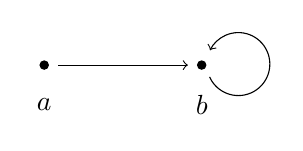
\begin{tikzpicture}
\draw[fill] (0,0) circle (1.5pt);
\draw[fill] (2,0) circle (1.5pt);
\draw[->,shorten >= 5pt, shorten <= 5pt] (0,0) -- (2,0);
\node at (0,-.5) {$a$};
\node at (2,-.5) {$b$};
\draw[->] (2.1,-.15) arc (204:204+310:4mm);
\end{tikzpicture}
\end{center}
De atomaire formule $R(a,b)$ is waar in een situatie als de met $a$ en $b$ aangeduide objecten in een relatie staan die met $R$ overeenkomt. De (binaire) relatie $R$ is met pijlen weergegeven. In dit geval is $R(a,b)$ waar: er gaat een pijl van $a$ naar $b$. Ook kunnen we kijken of samengestelde formules waar zijn in deze structuur:
\begin{itemize}
    \item $\exists y\;R(a,y)$ is waar, want de keuze van $b$ voor $y$ voldoet.
    \item $\forall x\;R(x,x)$ is onwaar, want $(a,a)$ behoort niet tot de pijlrelatie.
    \item $\exists y\forall x\;R(x,y)$ is waar, want neem voor $y$ eens $b$, dan gaat zowel van $a$ als van $b$ een pijl naar $b$.
\end{itemize}
\end{example}
Er is een verschil tussen de objecten $a$ en $b$ in de figuur, waarvan we kunnen \textit{zien} dat ze verschillen, en de constanten $a$ en $b$ in de logische taal, die best hetzelfde object zouden kunnen aanduiden. De constanten in de taal zijn de \textit{namen} die we aan de objecten toekennen. (Net zoals in de propositielogica propositieletters proposities uitdrukken, en in de predikaatlogica predikaatsymbolen predikaten aangeven.) We hadden best $a$ en $b$ hetzelfde object \textit{kunnen} laten aanduiden. Dit zou net als bij pseudoniemen zijn: `Paul Haenen', `Margreet Dolman' en `Dominee Gremdaat' zijn namen voor dezelfde persoon. In de logica zijn constanten namen voor objecten, en hetzelfde object kan met verschillende namen worden aangeduid.

Met connectieven kan nog steeds gerekend worden zoals in de propositielogica. Zo is in de situatie van voorbeeld \ref{vb:pred:model} de formule $R(a,b)\wedge R(b,b)$ waar, omdat $R(a,b)$ en $R(b,b)$ beide waar zijn, terwijl $R(a,b)\rightarrow R(b,a)$ onwaar is; er gaat immers wel een pijl van $a$ naar $b$, maar niet eentje van $b$ naar $a$. Vervolgens kunnen we kwantoren en connectieven weer in formules combineren: $\forall y(\exists x\;R(x,y)\rightarrow R(y,y))$ is waar in de situatie van voorbeeld \ref{vb:pred:model}, want als $y=a$, dan is $\exists x\;R(x,y)$ onwaar en dus de implicatie waar, en als $y=b$, dan zijn $\exists x\;R(x,y)$ en $R(y,y)$ beide waar en ook dan is de implicatie waar.

Een situatie als in voorbeeld \ref{vb:pred:model} heet in de logica een \textit{model}. We kunnen deze notie zien als de generalisering van het begrip waardering in de propositielogica\footnote{\textit{Waardering} in propositielogica is de (systematisch) toekenning van waarheidswaarden aan de propositieletters om zodoende te laten zien dat een formule waar danniet onwaar is; zodoende is elke rij van een waarheidstabel dus een waardering, waarvoor de waarheid van de formule waarvoor de tabel gemaakt wordt geanalyseerd.} (en het is net als inde propositielogica gebruikelijk `model' relatief ten opzichte van een formule, of een verzameling formules, te gebruiken: een situatie is \textit{model} van een formule als de formule daarin waar is). Een model bestaat uit een verzameling objecten waarop een aantal relaties en bewerkingen zijn gegeven die overeenkomen met de predikaat en functiesymbolen. Ook moeten we aangeven welk object uit de gegeven verzameling staat voor welke constante. We laten door middel van een aantal voorbeelden zien hoe modellen werken, en geven geen echte definitie.

Een atomaire formule zoals $R(a,b)$ is \textit{waar} in een model $\mathcal M$ als, gegeven de vertaalsleutel voor $a, b$ en $R$, de met $R$ in $\mathcal M$ corresponderende relatie geldt tussen de in $\mathcal M$ met $a$ en $b$ corresponderende objecten (en net zo voor variabele objecten $x$ en $y$). Een formule $\exists x\;\varphi$ is waar als er een object in $\mathcal M$ is zodat $\varphi$ waar is als we de voorkomens van $x$ in $\varphi$ over dat object laten gaan. Een formule $\forall x\;\varphi$ is waar als dat voor alle objecten in $\mathcal M$ zo is. Als een formule $\varphi$ waar is in $\mathcal M$ dan noteren we dit als $\mathcal M \vDash \varphi$ (de formule volgt \emph{semantisch} uit het model.

\begin{example}
De modellen waarin we predikaatlogica interpreteren kunnen heel abstract zijn maar ook tamelijk concreet. Beschouw bijvoorbeeld het model $\mathcal M$ hierna.
\begin{center}
    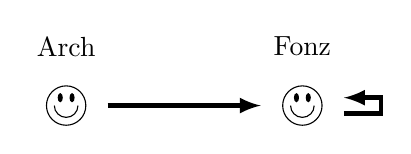
\begin{tikzpicture}
    \draw (0,0) circle (.25cm);
    \draw[fill] (-.075,.1) ellipse (.25mm and .5mm);
    \draw[fill] (.075,.1) ellipse (.25mm and .5mm);
    \draw (-.15,0) arc (180:180+180:1.5mm);
    \node at (0,.75) {Arch};
    \draw (3,0) circle (.25cm);
    \draw[fill] (3-.075,.1) ellipse (.25mm and .5mm);
    \draw[fill] (3+.075,.1) ellipse (.25mm and .5mm);
    \draw (3-.15,0) arc (180:180+180:1.5mm);
    \node at (3,.75) {Fonz};
    \draw[ultra thick,->, shorten <= 15pt, shorten >= 15pt,>=latex] (0,0) -- (3,0);
    \draw[ultra thick, shorten <= 15pt, shorten >= 15pt,->,>=latex] (3, -.1) -- (4, -.1) -- (4, .1) -- (3,.1);
    \end{tikzpicture}
\end{center}
Dit is eigenlijk hetzelfde model als in voorbeeld \ref{vb:pred:model}. Alleen is het linkerobject hier Arch en het rechterobject hier Fonz. Maar Arch en Fonz hadden we net zo goed $a$ en $b$ kunnen noemen. De binaire relatie $R(x,y)$ staat nu voor `persoon $x$ kent persoon $y$'. De drie andere formules in voorbeeld \ref{vb:pred:model} kunnen we nu ook een concretere interpretatie geven:
\begin{itemize}
    \item $\mathcal M \vDash \exists y\;R(a,y)$: `Arch kent iemand'. Dit is waar, want Arch kent Fonz.
    \item $\mathcal M \not\vDash \forall x\;R(x,x)$: `Iedereen kent zichzelf'. Dit is onwaar, want Arch kent zichzelf niet, alleen Fonz kent zichzelf.
    \item $\mathcal M \vDash \exists y\forall x\;R(x,y)$: `Er is iemand die door iedereen gekend wordt'. Dit is waar, want het gaat op voor Fonz.
\end{itemize}
\end{example}

Wanneer er ook nog sprake is van een eenplaatsig predikaatsymbool $P$ (een \textit{eigenschap}), dan geven we behalve pijlen ook gebieden in het model aan (waarin de objecten liggen die de eigenschap hebben) of we markeren de punten die aan een bepaalde eigenschap voldoen afzonderlijk.

\begin{example}\label{vb:pred:model:prop}
We gaan van een aantal formules na of ze waar of onwaar zijn in het model $\mathcal M$ hierna. Dit $\mathcal M$ verbeeldt twee objecten, een eigenschap en een relatie. Object $a$ heeft de eigenschap $P$, wat we aangeven met een open rondje, en de relatie $\{(a,a), (a,b)\}$ komt met $R$ overeen.

\begin{center}
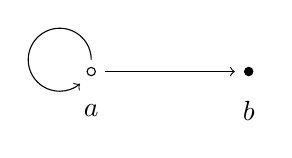
\begin{tikzpicture}
\draw (0,0) circle (1.5pt);
\draw[fill] (2,0) circle (1.5pt);
\draw[->,shorten >= 5pt, shorten <= 5pt] (0,0) -- (2,0);
\node at (0,-.5) {$a$};
\node at (2,-.5) {$b$};
\draw[->] (0,.15) arc (0:0+310:4mm);
\end{tikzpicture}
\end{center}
\begin{itemize}
    \item $\mathcal M \vDash \exists x(P(x)\wedge R(x,x))$\\
    Dit is waar. Ken aan $x$ $a$ toe, dan zien we dat $P(a)$ geldt (object $a$ heeft de eigenschap $P$) en dat $(a,a)\in R$ (de relatie $R$ bestaat tussen $a$ en zichzelf).
    \item $\mathcal M \not\vDash \forall x\exists y\;R(x,y)$\\
    Dit is onwaar. Ken aan $x$ $b$ toe. Er is geen uitgaande pijl van $b$ (er is geen pijl van $b$ naar $b$, en er is ook geen pijl van $b$ naar $a$). Kennelijk is $\exists y\;R(x,y)$ onwaar als $x$ gelijk aan $b$ is. Het geldt dus niet voor alle $x$ dat $\exists y\;R(x,y)$ waar is. Dus $\forall x\exists y\;R(x,y)$ is onwaar.
    \item $\mathcal M \vDash \forall x(P(x)\rightarrow\exists y\;R(x,y))$\\
    Dit is waar. We moeten iets aantonen voor alle $x$. Aan $x$ kunnen we $a$ toekennen, maar ook $b$. In het eerste geval heeft het object de eigenschap $P$, en moeten we laten zien dat er een $y$ is zodat $R(x,y)$. En die is er: ken $b$ aan $y$ toe. In het tweede geval geldt de implicatie omdat het object de eigenschap $P$ niet heeft: $P(b)$ is immers onwaar.
    \item $\mathcal M \vDash \forall x(R(x,x)\rightarrow(P(x)\wedge \exists y(R(x,y)\wedge\neg P(y))))$\\
    Dit is eveneens waar. Je kan zelf de verificatie uitvoeren.
\end{itemize}
Het grappige is dat in deze vier formules $a$ en $b$ nergens genoemd worden, maar dat we er \textit{toch} betekenis aan kunnen geven. Dit zien we vaak in de predikaatlogica.
\end{example}

\begin{example}
Ook in het geval van voorbeeld \ref{vb:pred:model:prop} kunnen we een iets beeldender interpretatie kiezen. Kijk maar eens naar de figuur hierna, die verbeeldt dat: Arch heeft haar, Arch kent zichzelf, en Arch kent Fonz.
\begin{center}
    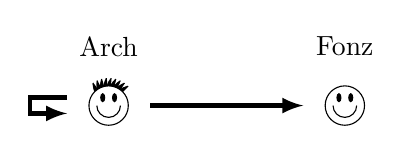
\begin{tikzpicture}
    \draw (0,0) circle (.25cm);
    \draw[fill] (-.075,.1) ellipse (.25mm and .5mm);
    \draw[fill] (.075,.1) ellipse (.25mm and .5mm);
    \draw (-.15,0) arc (180:180+180:1.5mm);
    \node at (0,.75) {Arch};
    \foreach \x in {45,55,...,134} \draw (\x:0.25cm) -- (\x:0.35cm);
    \foreach \x in {46,56,...,134} \draw (\x:0.25cm) -- (\x:0.34cm);
    \foreach \x in {47,57,...,134} \draw (\x:0.25cm) -- (\x:0.33cm);
    \foreach \x in {48,58,...,134} \draw (\x:0.25cm) -- (\x:0.32cm);
    \foreach \x in {49,59,...,134} \draw (\x:0.25cm) -- (\x:0.31cm);
    \foreach \x in {50,60,...,134} \draw (\x:0.25cm) -- (\x:0.30cm);
    \foreach \x in {51,61,...,134} \draw (\x:0.25cm) -- (\x:0.29cm);
    \foreach \x in {52,62,...,134} \draw (\x:0.25cm) -- (\x:0.28cm);
    \foreach \x in {53,63,...,134} \draw (\x:0.25cm) -- (\x:0.27cm);
    \foreach \x in {54,64,...,134} \draw (\x:0.25cm) -- (\x:0.26cm);
    \draw (3,0) circle (.25cm);
    \draw[fill] (3-.075,.1) ellipse (.25mm and .5mm);
    \draw[fill] (3+.075,.1) ellipse (.25mm and .5mm);
    \draw (3-.15,0) arc (180:180+180:1.5mm);
    \node at (3,.75) {Fonz};
    \draw[ultra thick,->, shorten <= 15pt, shorten >= 15pt,>=latex] (0,0) -- (3,0);
    \draw[ultra thick, shorten <= 15pt, shorten >= 15pt,->,>=latex] (0, .1) -- (-1, .1) -- (-1, -.1) -- (0,-.1);
    \end{tikzpicture}
\end{center}
De formules van voorbeeld \ref{vb:pred:model:prop} zijn hier natuurlijk eveneens waar/onwaar. Voor de interpretatie kunnen we bedenken (voor `object' nemen we nu gemakshalve `man'):
\begin{itemize}
    \item $\mathcal M \vDash \exists x(P(x)\wedge R(x,x))$\\
    ``Er is een behaarde man die zichzelf kent.'' Dit is waar: Arch.
    \item $\mathcal M \not\vDash \forall x\exists y\;R(x,y)$\\
    ``Iedereen kent iemand.'' Dit is onwaar. Fonz kent niemand.
    \item $\mathcal M \vDash \forall x(P(x)\rightarrow\exists y\;R(x,y))$\\
    ``Iedere behaarde man kent iemand.'' Dit is ook waar. Arch heeft haar en kent Fonz.
    \item $\mathcal M \vDash \forall(R(x,x)\rightarrow(P(x)\wedge\exists y(R(x,y)\wedge\neg P(y))))$\\
    ``Iedereen met zelfkennis is behaard en kent een kale.''
\end{itemize}
\end{example}

Tot nu gaven we een model $\mathcal M$ en bekeken dan welke formules waar waren. Soms zijn we meer in een andere vraag ge\"interesseerd: gegeven een formule, verzin een model $\mathcal M$ dat deze formule waar (of juist onwaar) maakt. Als dit lukt noemen we de formule vervulbaar\footnote{Merk op dat, terwijl het vinden van een model de vervulbaarheid van een formule aantoont, het vinden van een model dat een formule onwaar maakt, niet de \textit{onvervulbaarheid} van die formule aantoont!}. Dit gaat dus net als in de propositielogica: een formule is vervulbaar als ze een model heeft.

\begin{example}
De formule $\forall x\exists y\;R(x,y)$ is waar in het model van voorbeeld \ref{vb:pred:model} en onwaar in het model van voorbeeld \ref{vb:pred:model:prop}. Voor formule $\forall x\forall y(R(x,y)\rightarrow R(x,x))$ is het omgekeerde het geval: deze is onwaar in het model van voorbeeld \ref{vb:pred:model} en waar in het model van voorbeeld \ref{vb:pred:model:prop}. Ze is onwaar in het eerste model, want neem namelijk $x=a$ en $y=b$, dan is $R(a,b)\rightarrow R(a,a)$ onwaar.

Maar ze is waar in het laatste model, want neem namelijk $x=a$ dan zijn $R(a,a)\rightarrow R(a,a)$ en $R(a,b)\rightarrow R(a,a)$ beide waar en voor $x=b$ zijn ook $R(b,a)\rightarrow R(b,b)$ en $R(b,b)\rightarrow R(b,b)$ beide waar. Beide formules zijn dus vervulbaar.
\end{example}

Tot nu toe hebben we het alleen over modellen voor gesloten formules gehad. Wat te doen met vrije variabelen? Anders dan voor een constante, ligt de waarde van een (vrije) variabele niet vast door het model. Om te kunnen vaststellen of de formule in zo'n geval waar is, moeten de waarden van de vrije variabelen expliciet worden aangegeven. Zo is $P(x)\wedge\exists y\;R(x,y)$ waar in het model van voorbeeld \ref{vb:pred:model:prop} als $x=a$, maar onwaar als $x=b$.
\begin{example}
Beschouw het volgende model. Het bestaat uit de getallen 2, 3, 4 en 5 met de `kleiner dan'-relatie en de priemgetaleigenschap.
\begin{center}
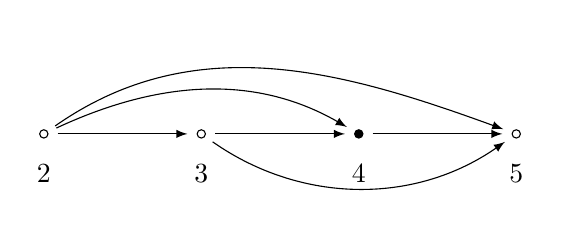
\begin{tikzpicture}
\draw (0,0) circle (1.5pt);
\draw (2,0) circle (1.5pt);
\draw[fill] (4,0) circle (1.5pt);
\draw (6,0) circle (1.5pt);
\draw[->,shorten >= 5pt, shorten <= 5pt,>=latex] (0,0) -- (2,0);
\draw[->,shorten >= 5pt, shorten <= 5pt,>=latex] (2,0) -- (4,0);
\draw[->,shorten >= 5pt, shorten <= 5pt,>=latex] (4,0) -- (6,0);
\node at (0,-.5) {$2$};
\node at (2,-.5) {$3$};
\node at (4,-.5) {$4$};
\node at (6,-.5) {$5$};
\draw[->,shorten <= 5pt, shorten >= 5pt,out=25,in=150,>=latex] (0,0) to (4,0);
\draw[->,shorten <= 5pt, shorten >= 5pt,out=35,in=160,>=latex] (0,0) to (6,0);
\draw[->,shorten <= 5pt, shorten >= 5pt,out=325,in=215,>=latex] (2,0) to (6,0);
\end{tikzpicture}
\end{center}
De constanten 2, 3, 4 en 5 zijn gewoon door die getallen weergegeven. De eigenschap $P$ staat voor `priemgetal' (en is weergegeven door een open rondje). Neem nu de formule $x<5\rightarrow P(x)$. Deze is waar als $x=3$, omdat $3<5$ en 3 een priemgetal is. De formule is daarentegen onwaar als $x=4$, omdat $4<5$ maar 4 is geen priemgetal is. Maar als $x=5$ is de formule waar: 5 is immers \textit{niet} (echt) kleiner dan 5. Voor de waarheid van de implicatie maakt het verder niet uit dat 5 een priemgetal is.
\end{example}

\begin{example}
Hoewel de nadruk tot zover heeft gelegen op eindige modellen, zijn ook oneindige modellen mogelijk. De verzameling van natuurlijke getallen $\mathbb{N}=\{0, 1, 2, 3, 4, \ldots\}$ is het schoolvoorbeeld van een oneindige verzameling. Vat in dit model het predikaatsymbool $P$ op als de verzameling priemgetallen $\{2,3,5,7,11,\ldots\}$, het predikaatsymbool $E$ als de verzameling even natuurlijke getallen $\{0,2,4,6,8,\ldots\}$, en de tweeplaatsige predikaatsymbolen $>$ en $\leq$ als de groter-dan-relatie respectievelijk kleiner-dan-of-gelijk-relatie. Op dit model zijn bijvoorbeeld de volgende formules waar:
$$\forall x(E(x)\rightarrow\exists y((y>x)\wedge E(y)))$$
$$\forall x(P(x)\rightarrow\exists y((y>x)\wedge P(y)))$$
Onwaar zijn:
$$\forall x(E(x)\vee P(x))$$
$$\forall x(P(x)\rightarrow P(x+2))$$
Het functiesymbool `$+$'wordt hier opgevat als gewone optelling. Ten slotte zijn er nog formules waarvan de waarheid onbekend is, zoals het vermoeden van Goldbach:
$$\forall x((E(x)\wedge x>2)\rightarrow\exists y\exists z(P(y)\wedge P(z)\wedge x=y+z))$$
Zoals eerder gezegd staan we in de predikaatlogische taal ook uitdrukkingen als $x+y$ toe als term.
\end{example}

\section{Predikaatlogische wetten en logisch gevolg}
 Net als voor de propositielogica kunnen we ook voor de predikaatlogica \textit{logisch gevolg} en \textit{logische equivalentie} defini\"eren -- met letterlijk dezelfde formuleringen als in hoofdstuk \ref{ch:proposities}. We kunnen dan laten zien dat, bijvoorbeeld, alle vier de volgende formuleringen precies hetzelfde uitdrukken, namelijk dat er geen grootste priemgetal is (zie het voorbeeld aan het begin van sectie \ref{sec:pred:semantiek}):
 \begin{itemize}
     \item $\forall x(P(x)\rightarrow\exists y(P(y)\wedge y>x))$
     \item $\forall x\exists y(P(x)\rightarrow(P(y)\wedge y>x))$
     \item $\forall x\exists y(\neg P(x)\vee(P(y)\wedge y>x))$
     \item $\forall x\exists y((P(x)\rightarrow P(y))\wedge((P(x)\rightarrow y>x))$
 \end{itemize}
 Een voorbeeld van een algemene predikaatlogische wet, die we informeel inmiddels al wel toegepast hebben, is dat $\neg\exists x\;\varphi$ equivalent is met $\forall x\;\neg\varphi$. Met zo'n regel, en nog een variatie erop, kunnen we aantonen dat $\forall x\exists y\;x<y$, voor `er is geen grootste getal', logisch equivalent is met de formule $\neg\exists x\forall y\;x\geq y$ - we gebruiken daarin tevens dat $\neg(x<y)$ equivalent is met $x\geq y$.
 
 Met de notie van \textit{predikaatlogisch gevolg} kunnen we formeel laten zien dat een eeuwenoude redenering inderdaad geldig is:
 $$\forall x(M(x)\rightarrow S(x)), M(s)\Rightarrow S(s)$$
 Deze formule formaliseert de redenering `Alle mensen zijn sterfelijk. Socrates is een mens. Dus Socrates is sterfelijk.'
 
 Een volgend voorbeeld van een standaard predikaatlogisch gevolg  is $\exists x\forall y\;\varphi\Rightarrow\forall y\exists x\;\varphi$\footnote{Maak zelf een model om dit te verifi\"eren.}. Maar in de andere richting is dit nu juist ongeldig: neem bijvoorbeeld voor $\varphi$ de atomaire formule $y>x$ en als model de natuurlijke getallen, dan is $\forall y\exists x\;x>y$ het geval want bij ieder natuurlijk getal is er nog een groter natuurlijk getal, bijvoorbeeld dat getal plus 1. Maar $\exists x\forall y\;x>y$ is onwaar, want er is geen grootste natuurlijk getal. Dus $\forall y\exists x\;x>y\not\Rightarrow\exists x\forall y\;x>y$.
 
 \section{Samenvatting}
 Voor het bepalen van de waarheidswaarde van een formule spelen in de predikaatlogica modellen dezelfde rol als waarderingen in de propositielogica. Een model is een structuur die bestaat uit een verzameling objecten waarop relaties (en in het bijzonder: eigenschappen) zijn gedefinieerd. De relaties komen overeen met de predikaatsymbolen van de formules waaraan we een waarheidswaarde willen toekennen. Objecten kennen we aan de constanten in de predikaatlogische taal toe. Verschillende constanten kunnen in een model hetzelfde object aanduiden, en een constante kan in verschillende modellen door verschillende objecten worden weergegeven. Voor variabelen kunnen we in een gegeven model verschillende waarden kiezen. Een formule $\forall x\;\varphi$ is waar als $\varphi$ geldt voor elk object dat we aan $x$ kunnen toekennen; $\exists x\;\varphi$ is waar als er ten minste \'e\'en zo'n object bestaat.
 
 \subsection{Opgaven}
 \begin{exercise}
 Stel we gebruiken het functiesymbool `$-$' voor de bewerking `aftrekken'. Als $E$ staat voor `is even' en `$P$' voor `is een priemgetal', wat drukken de volgende formules dan uit?
 \begin{enumerate}
     \item $\forall x((E(x)\wedge x>2)\rightarrow\exists y(P(y)\wedge P(x-y)))$
     \item $\neg\exists x(P(x)\wedge\forall y(P(y)\rightarrow y\leq x))$
 \end{enumerate}
 \end{exercise}
 
 \begin{exercise}
 Beschouw de formule $\forall x\forall y\forall z((R(x,y)\wedge R(y,z))\rightarrow R(x,z))$.
 \begin{enumerate}
     \item Is deze formule waar in een model $\mathcal M$ met de natuurlijke getallen als objecten, waarin $R$ overeenkomt met de gewone kleiner-dan-relatie ($<$)?
     \item En in een model $\mathcal N$ met dezelfde verzameling objecten, maar nu met de relatie $R$ gedefinieerd door: $R(x, y)$ precies dan als $x\leq y+1$?
     \item Is de formule waar in het model $\mathcal O$ uit voorbeeld \ref{vb:pred:model}?
     \item Is de formule waar in elk model $\mathcal P$ met precies twee objecten? Zo ja, bewijs dit, zo nee, geef een voorbeeld van een model met twee objecten waarop de formule niet waar is.
 \end{enumerate}
 \end{exercise}
 
\begin{exercise}
Beschouw het volgende model $\mathcal M$:
\begin{center}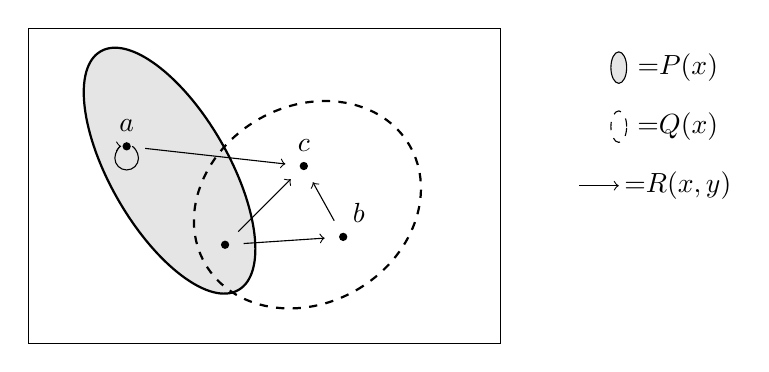
\begin{tikzpicture}
\draw (0,0) rectangle (6,4);
\draw[thick,fill=gray!20,rotate=30] (2.65,1) ellipse (.75cm and 1.75cm);
\draw[thick,dashed,rotate=-60] (.25,3.95) ellipse (1.25cm and 1.5cm);
\node[circle,fill,inner sep=0pt,minimum size=3pt,label={[anchor=south]north:$a$}] at (1.25, 2.5) (a) {};
\node[circle,fill,inner sep=0pt,minimum size=3pt] at (2.5, 1.25) (d) {};
\node[circle,fill,inner sep=0pt,minimum size=3pt,label={[anchor=south west]north:$b$}] at (4,1.35) (b) {};
\node[circle,fill,inner sep=0pt,minimum size=3pt,label={[anchor=south]north:$c$}] at (3.5,2.25) (c) {};
\draw[->,shorten <=2pt,shorten >=2pt] (a) arc(90:-270:.15); 
\draw[->,shorten <=5pt,shorten >=5pt] (a) -- (c); 
\draw[->,shorten <=5pt,shorten >=5pt] (d) -- (c); 
\draw[->,shorten <=5pt,shorten >=5pt] (d) -- (b); 
\draw[->,shorten <=5pt,shorten >=5pt] (b) -- (c);
\draw[fill=gray!20] (7.5,3.5) ellipse (.1cm and .2cm);\node at (8.25,3.5) {=$P(x)$};
\draw[dashed] (7.5,2.75) ellipse (.1cm and .2cm);\node at (8.25,2.75) {=$Q(x)$};
\draw[->] (7,2) -- (7.5,2);\node at (8.25,2) {=$R(x,y)$};
\end{tikzpicture}
\end{center}
Beredeneer welke van de volgende formules geldig zijn op $\mathcal M$:
\begin{enumerate}
    \item $\mathcal M \vDash R(a,a)$
    \item $\mathcal M \vDash R(x,x)$
    \item $\mathcal M \vDash \exists y\; R(a,y)$
    \item $\mathcal M \vDash \exists x\; R(x,x)$
    \item $\mathcal M \vDash \neg\forall x(P(x)\rightarrow R(x,x))$
    \item $\mathcal M \vDash \exists x(P(x)\wedge R(x,x))$
    \item $\mathcal M \vDash \forall x\exists y\;R(x,y)$
    \item $\mathcal M \vDash \forall x(R(x,x)\rightarrow P(x))$
    \item $\mathcal M \vDash \forall x\bigl[P(x)\rightarrow\exists y\;R(x,y)\bigr]$
    \item $\mathcal M \vDash \forall x\bigl[P(x)\rightarrow\exists y(R(x,y)\wedge Q(y))]$
\end{enumerate}
\end{exercise}

\begin{exercise}
Beschouw het domein $\mathbb{N}$ van natuurlijke getallen, met $E$ als het even-predikaat ($E(x)$ wil zeggen `$x$ is even') en een $A$ als optel-predikaat ($A(x,y,z)$ wil zeggen `$x+y=z$').

Geef aan of de volgende zinnen waar zijn op dit model:
\begin{enumerate}[label=\textit{\alph*.}]
\item $\forall x(E(x)\leftrightarrow\exists y\;A(y,y,x))$;
\item $\forall z\exists x\exists y(\neg(x=y)\wedge A(x,y,z))$;
\item $\forall x\forall y\forall z((E(x)\wedge E(y)\wedge A(x, y, z))\rightarrow E(z))$.
\end{enumerate}
\end{exercise}

\begin{exercise}
Gegeven is de volgende informatie over een model:\\
Predikaten $P,Q$ en $P$ is een-plaatsig, $Q$ is twee-plaatsig.\\
1 constante $c$.
$$A:= \forall x (P(x)\rightarrow\exists y\; Q(x,y))$$
\begin{enumerate}[label=\textit{\alph*.}]
\item Teken een model $\mathcal M$ waar deze formule waar is.
\item Teken een model $\mathcal N$ waar deze formule onwaar is.
\end{enumerate}
$$B:=(P(c)\wedge\forall x(P(x)\rightarrow\exists y(Q(x,y)\wedge P(y))))$$
\begin{enumerate}[label=\textit{\alph*.}]
\setcounter{enumi}{2}
\item Hoeveel elementen heb je minimaal nodig in een model om $B$ waar te maken?
\end{enumerate}
\end{exercise}


\part{Hardware}
\chapter{Computerarchitectuur}
Om efficiënte code voor data-analyse te schrijven, is het belangrijk om computerarchitectuur te begrijpen. Het snelheidsverschil tussen twee codes die hetzelfde resultaat berekenen, kan variëren van een paar procent tot een veelvoud, afhankelijk van hoe goed de algoritmen zijn afgestemd op de processorarchitectuur. Het is dus niet genoeg om een algoritme te hebben en het simpelweg op de computer te zetten: enige kennis van computerarchitectuur is aan te raden, soms zelfs cruciaal.

Met Turing Complete hebben we gezien hoe een computer opgebouwd kan worden uit niet veel meer dan logische-gates. We hebben toegewerkt naar een werkende computer, die met behulp van instructies (in de vorm van binaire getallen) te programmeren was. Door een set instructies in het geheugen te zetten en de CPU naar de eerste instructie te verwijzen kon een stappenplan worden uitgevoerd, waarna het resultaat ook weer ergens in het geheugen te lezen was.

De computer die we hebben opgebouwd is echter nog niet zo makkelijk te gebruiken als bijvoorbeeld je laptop. Bij het opstarten komt deze in een werkende omgeving terecht met Windows, Linux of MacOS, en kun je zelf software schrijven met bijvoorbeeld Python. Python is net als machine-code een manier om de computer te programmeren, maar werkt een stuk makkelijker: je kan met een enkele regel programmeercode complexe bewerkingen uitvoeren, en hoeft niet alles op CPU-niveau uit te denken. In dit hoofdstuk zullen we in grote lijnen zien hoe we deze twee werelden bij elkaar kunnen brengen: de hardware die denkt in enen en nullen, en de programmeur / gebruikers die liever in menselijke termen redeneren.

\section{De Von Neumann-architectuur}\label{sec:vonneuman }
Veel computerarchitecturen kunnen op een hoog niveau worden beschreven als \textit{Von Neumann-architecturen}. Dit beschrijft een ontwerp met een enkel geheugen dat zowel programma's als data opslaat, en een verwerkingseenheid die instructies uitvoert in een cyclus van "fetch, decode, execute, store".
  \begin{marginfigure}
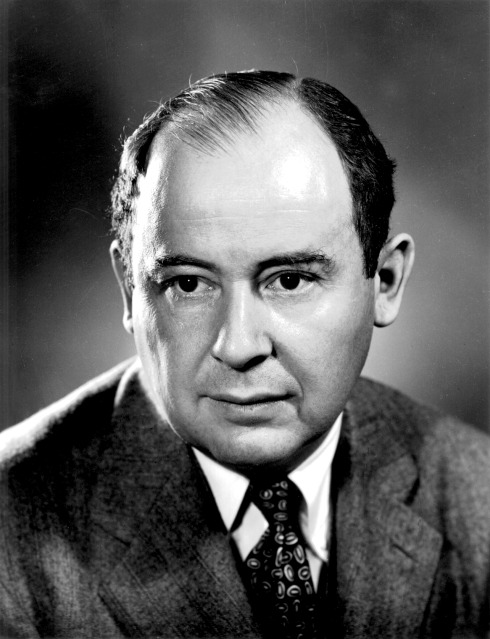
\includegraphics[width=0.6\textwidth]{JohnvonNeumann-LosAlamos.jpg}\\
    Jonh von Neumann {\scriptsize\emph (Image by Wikipedia)}\\[3mm]
  \end{marginfigure}

\begin{figure}[ht]
    \centering
    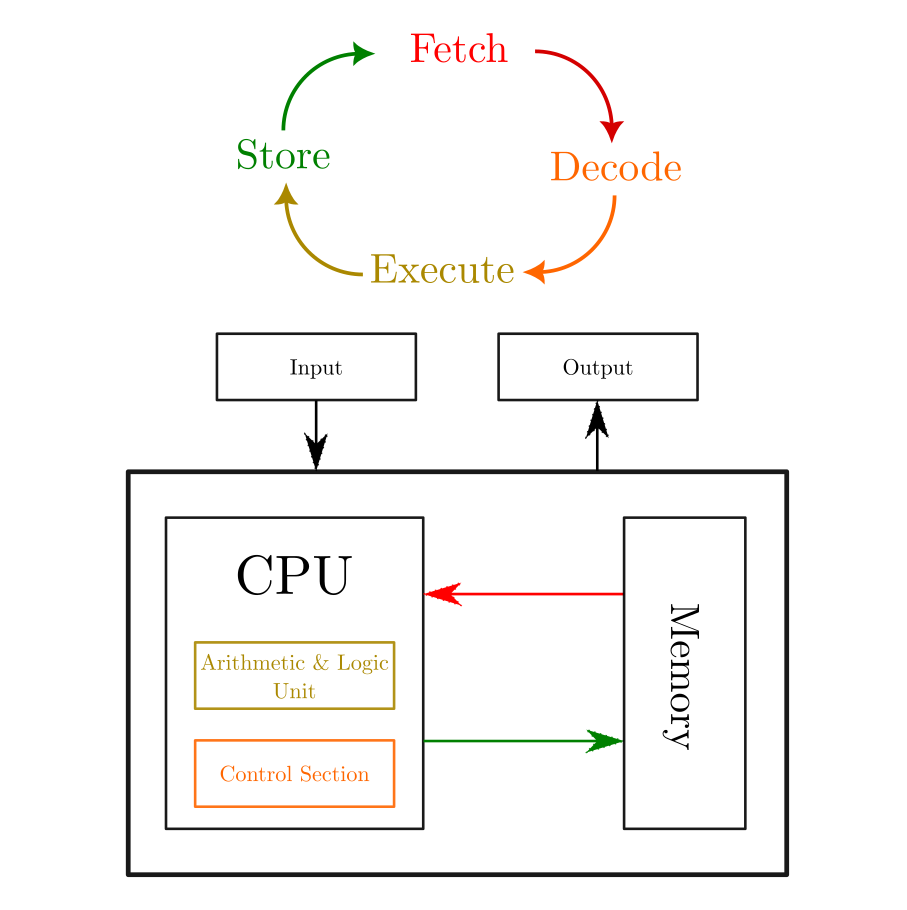
\includegraphics[width=0.6\textwidth]{neumann.png}
    \caption{Von Neumann-architectuur en -cyclus}
    \label{fig:neumann}
\end{figure}

Dit model onderscheidt moderne processors van de allereerste ontwerpen, waarbij het programma vast was ingebakken. Het stelt programma's ook in staat om zichzelf aan te passen of andere programma's te genereren, omdat instructies en data in hetzelfde geheugen worden opgeslagen.

In data-analytisch rekenwerk richten we ons meestal niet op programmacode, maar voornamelijk op data en hoe deze tijdens de uitvoering van het programma wordt verplaatst. Voor de meeste praktische doeleinden is het alsof programma en data apart worden opgeslagen.

\section{Moderne processors}\label{sec:fp }
Moderne processors zijn behoorlijk complex. In tegenstelling tot het Von Neumann-model, waarin één entiteit instructies uitvoert, hebben moderne processors vaak meerdere \textit{cores}, die onafhankelijk van elkaar instructies kunnen uitvoeren. Bovendien gebruiken processors vaak \textit{out-of-order execution}, waarbij instructies in een andere volgorde kunnen worden uitgevoerd dan in het programma is gespecificeerd, zolang het resultaat maar hetzelfde blijft.

\subsection{8-bit, 16-bit, 32-bit, 64-bit}
Processors worden vaak gekarakteriseerd door de grootte van de data-eenheden die ze kunnen verwerken. Dit kan betrekking hebben op:
\begin{itemize}
\item De breedte van het pad tussen processor en geheugen.
\item De manier waarop geheugen wordt geadresseerd.
\item Het aantal bits in een register, wat overeenkomt met de grootte van een data-eenheid die de CPU\sidenote{Central Processing Unit, oftewel processor.} tegelijkertijd kan verwerken.
\item De grootte van een floating-point getal.
\end{itemize}

\noindent Tegenwoordig zijn 64-bit processors de norm.

\section{Geheugenhiërarchie}\label{sec:hierarchy }
In de Von Neumann-architectuur wordt data direct vanuit het geheugen naar de processor geladen, waar het wordt verwerkt. Dit beeld is echter onrealistisch vanwege de zogenaamde \textit{memory wall}: het geheugen is te traag om data snel genoeg naar de processor te sturen. In werkelijkheid zijn er verschillende geheugenniveaus tussen de processor en het hoofdgeheugen, zoals registers en caches, die samen de \textit{geheugenhiërarchie} vormen. Deze omvat, van \emph{klein-maar-snel} naar \emph{groot-maar-traag} de registers, het cache-geheugen, met RAM geheugen en de permanente opslag zoals SSDs en harde schijven.

\subsection{Bussen}
De draden die data door een computer verplaatsen, worden \textit{bussen} genoemd. De belangrijkste bus voor ons is de \textit{Front-Side Bus} (FSB), die de processor met het geheugen verbindt. Deze bus is meestal langzamer dan de processor, wat een van de redenen is waarom caches nodig zijn.

\subsection{Latentie en bandbreedte}\label{sec:latencybandwidth }
Er zijn twee belangrijke concepten om de beweging van data te beschrijven: \textit{latentie} en \textit{bandbreedte}.
\begin{description}
\item[Latentie] is de vertraging tussen het moment waarop de processor een verzoek voor een gegevensitem doet en het moment waarop het item daadwerkelijk aankomt. Lage latentie is belangrijk om te voorkomen dat de processor moet wachten op data.
\item[Bandbreedte] is de snelheid waarmee data aankomt na de initiële latentie. Bandbreedte wordt gemeten in bytes per seconde of per klokcyclus.
\end{description}

Deze concepten zijn belangrijk omdat ze de prestaties van algoritmen kunnen beïnvloeden. Zonder caches kan de prestaties van een algoritme worden beperkt door de snelheid van het geheugen.

\subsection{Registers}\label{sec:register }
Elke processor heeft een kleine hoeveelheid intern geheugen: de \textit{registers}. Registers zijn waar de processor daadwerkelijk op werkt. Het verplaatsen van data naar en vanuit registers is essentieel instantaan, wat ze zeer snel maakt.

Het is belangrijk om data zoveel mogelijk in registers te houden, vooral in binnenste lussen van een programma, om de prestaties te verbeteren.

\subsection{Caches}\label{sec:cache }
Tussen de registers en het hoofdgeheugen bevinden zich verschillende niveaus van \textit{cache}-geheugen, die sneller zijn dan het hoofdgeheugen maar kleiner in omvang. Caches helpen om data die recentelijk is gebruikt sneller toegankelijk te maken.

Er zijn meestal meerdere cache-niveaus, zoals L1, L2 en soms L3. L1-cache is het snelst maar het kleinst, terwijl L2 en L3 groter maar langzamer zijn. Het vinden van data in de cache wordt een \textit{cache hit} genoemd, terwijl het niet vinden ervan een \textit{cache miss} wordt genoemd.

Caches zijn belangrijk omdat ze de prestaties van algoritmen kunnen verbeteren door data sneller beschikbaar te maken. Het is echter belangrijk om te programmeren op een manier die het gebruik van caches maximaliseert.


\section{Het Operating System}\label{sec:os}

De software die je als (AI)-programmeur schrijft, zal in de regel niet direct op de hardware draaien, maar binnen de omgeving van een \emph{operating system} (OS). Dit is een stuk software\sidenote{Voorbeelden zijn Linux, MacOS en Windows, maar ook mobiele systemen zoals Android en iOS.} dat tijdens het opstarten van de computer als eerste wordt gestart, en dient als abstractielaag tussen de hardware en de user-software. Het is zo opgezet dat het enerzijds met de specifeke hardware overweg kan, en anderzijds eenzelfde basis biedt voor software (ongeacht wat de onderliggende hardware is). Zonder dit OS zou je als programmeur zelf alle details van de computer-hardware moeten managen, waardoor je telkens weer veel (foutgevoelige) code nodig hebt om simpele taken te kunnen programmeren. Denk hierbij aan het opslaan van data, het afwisselen van meerdere taken, of het weergeven van een interface op het scherm. Complexe software zoals een web-browser of office-suite zijn zonder de abstractie van een OS vrijwel onmogelijk te programmeren, en als het al lukt specifiek voor één systeem gemaakt. Met het OS is er een basis waar complexe software op gemaakt kan worden. Het OS heeft doorgaans de volgende taken:

\begin{itemize}
\item Abstractie van de hardware t.b.v. user processes
\item Aansturen randapparatuur / IO
\item Processen laden en managen / scheduling
\item Beheren system resources (e.g.~memory, CPU-tijd)
\item Leveren van het filesystem
\end{itemize}

De meesten code die wij als AI-ers schrijven zal draaien in een hogere taal zoals Python, die onze instructies vertaalt naar iets waar het operating system mee kan werken. Het OS vertaalt dit vervolgens naar de specifieke hardware.


\section{Geheugensegmenten}\label{geheugensegmenten}

Hoewel we het inmiddels een paar keer over processen hebben gehad,
leggen we voor nu de nadruk nog even op een computer met een enkele
taak. Moderne computers draaien vaak vele taken tegelijk\sidenote{Of heel snel afgewisseld, waardoor het wel tegelijk lijkt.}, maar het Operating System zorgt ervoor dat deze taken van elkaar afgeschermd zijn en dat het vanuit een proces lijkt alsof deze de hele computer ter beschikking heeft en geen rekening met anderen hoeft te houden.

\newthought{Het geheugen van een proces} is opgedeeld in een aantal segmenten. De eerste sectie is Text en bevat de instructies van het proces. Dit gedeelte van het geheugen is na het inladen van het proces read-only: als alle code is geladen mag deze in het kader van de veiligheid niet meer veranderd worden. Na de instructies volgen de Data en BSS segmenten. Data bevat alle globale en statische variabelen met een initiele waarde. Deze worden buiten functies gedefinieerd of zijn als static (onveranderbaar) gemarkeerd. BSS (historisch: Block Started by Symbol) bevat de statische variabelen die wel defined, maar niet geïnitialiseerd zijn. Na de BSS volgen de heap en de stack, die in de volgende sectie besproken worden. Beide kunnen hun formaat dynamisch aanpassen. De stack en heap beginnen leeg en groeien naar elkaar toe. Bij het gebruik van een high-level programmeertaal zoals Python heb je als programmeur vaak geen directe invloed op wat waar in het geheugen komt: dit wordt door de Python-interpreter gemanaged.

\begin{figure}[ht]
    \centering
    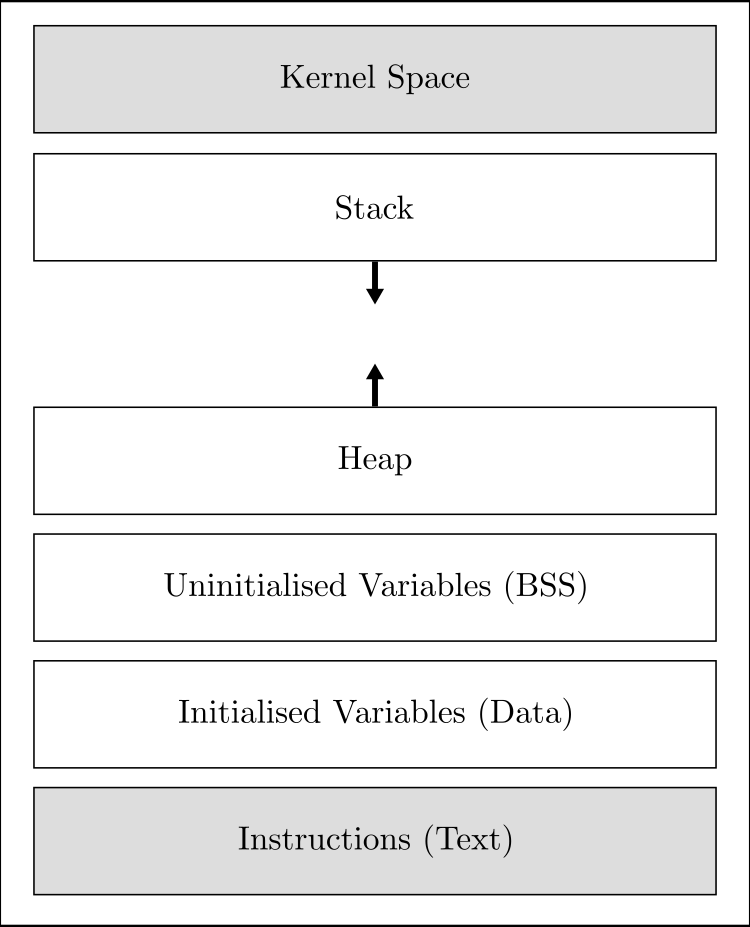
\includegraphics[width=0.4\textwidth]{process.png}
    \caption{Geheugenmodel Proces}
    \label{fig:process-memory}
\end{figure}

\subsection{De Stack}
De stack wordt gebruikt om \emph{function calls} mogelijk te maken: het aanroepen van een functie. Op het moment dat dit gebeurt wordt er een nieuw stuk van het geheugen uitgevoerd (dus niet simpelweg de volgende instructie). Dit betekent dat de oude variabelen even niet meer toegankelijk moeten zijn, en dat daar mogelijk nieuwe variabelen voor in de plaats komen. Ook moet bekend zijn waar de software gebleven was, zodat die nadat de functie beëindigd is weer op de juiste plek verder kan. Als de functie wordt aangeroepen, wordt een frame aangemaakt. Dit frame bevat de parameters van de functieaanroep, het adres van waaraf de functie werd aangeroepen (return address), lokale variabelen en soms het formaat van het frame of de vorige waarde van de stack pointer (zodat bekend is welke bytes per \emph{pop} gelezen moeten worden, wanneer frames geen vast formaat hebben). Hierna kan met behulp van een \texttt{JUMP}-instructie naar de functie-instructies gesprongen worden. Als een functiecall klaar is dan keert de computer terug naar de instructie direct na de functieaanroep. Deze is te vinden doordat het return adres in het frame op de stack staat opgeslagen. Zodra de computer het return adres nodig heeft wordt het frame gepopt, en wordt de stack meteen een frame kleiner.

\begin{aside}[De Stack]\label{de-stack}
Een stack (stapel) is een datastructuur waar dynamisch informatie aan toegevoegd of uitgehaald kan worden. De stack werkt volgens het \textbf{Last in, first out} principe, en wordt daarom ook wel de LIFO genoemd. De stack begint leeg, waarna hier data aan kan worden toegevoegd. Nieuwe data wordt bovenop de stack gezet (dit heet een \textbf{push}), en alleen het bovenste element van de stack is zichtbaar. Als het bovenste element gelezen wordt, wordt het meteen van de stack verwijderd (dit een heet \textbf{pop}). Ook in het geheugen wordt gebruik gemaakt van een stack. De stack heeft als voordeel dat je altijd de meest recente informatie bovenaan hebt.\\[3mm]
\begin{figure}[ht]
    \centering
    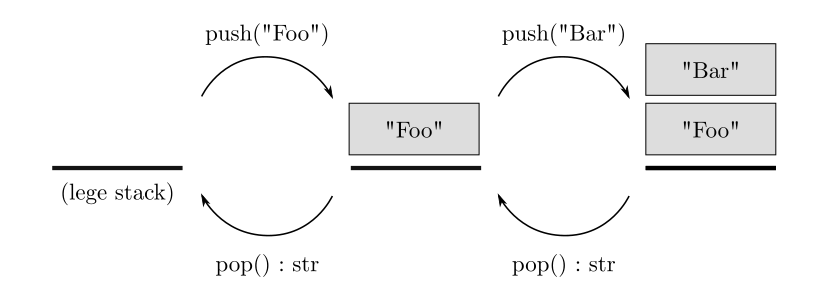
\includegraphics[width=\textwidth]{stack-structure.png}
    \caption{De Stack als datastructuur}
    \label{fig:stack}
\end{figure}
\end{aside}


De stack heeft een maximale grootte. Bij simpele systemen kan dit komen door een beperkte hoeveelheid geheugen, in complexere systemen met meerdere processen is er een maximum vastgesteld. Als dit maximum bereikt wordt, spreken we van een stack overflow, en wordt de executie van het programma onderbroken (met andere woorden: een crash!). Het maximumformaat van de stack is doorgaans vrij groot, een stack overflow wordt dan ook meestal door een programmeerfout veroorzaakt. Het meest simepele voorbeeld is een functie die zichzelf herhaaldelijk aanroept (recursie). Recursie is in principe geen probleem (en in sommige gevallen zelfs de meest nette oplossing) maar als een functie altijd zichzelf aan blijft roepen (en niet na een beperkt aantal keren returnt) dan hebben we een oneindige loop waarbij de stack snel volgezet wordt. Bij een beperktere recursie wordt ook een stack opgebouwd, maar op een gegeven moment zal de laatste aanroep returnen, waarna de aanroep daarvoor returnt, etc. en de stack ook weer wordt afgebroken.

\begin{figure}[ht]
    \centering
    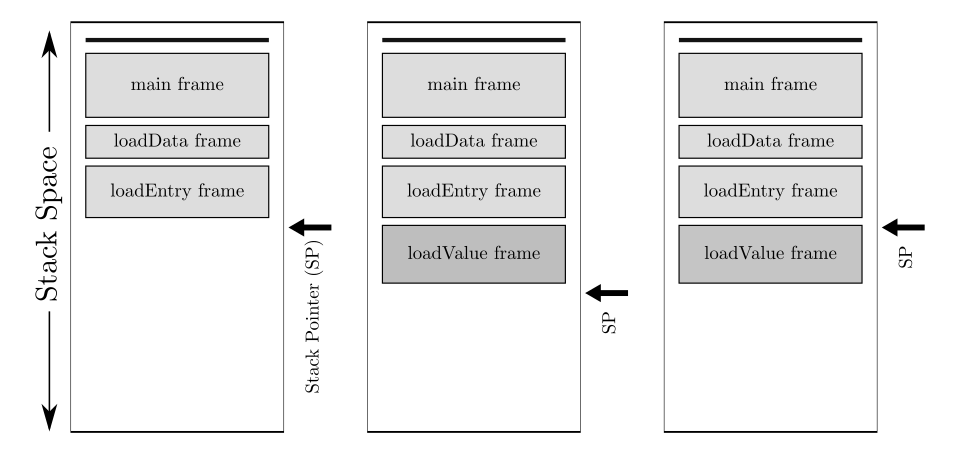
\includegraphics[width=\textwidth]{mem-stack.png}
    \caption{De Stack in het geheugen}
    \label{fig:stack}
\end{figure}

\subsection{De Heap}\label{de-heap}

Waar BSS en Data voor statische data gebruikt wordt, is de heap voor dynamische data: data waarvan tijdens het programmeren en compilen nog niet bekend is hoeveel ruimte ervoor nodig is. De heap wordt tijdens het uitvoeren van de code expliciet toebedeeld (gealloceerd).

\begin{itemize}
\item Dynamische alloceerbaar
\item Expliciet ruimte reserveren
\item Na gebruik vrijgeven
\end{itemize}

Voor gebruik van de heap geeft software aan het operating system aan hoeveel\sidenote{Hoewel de hoeveelheid benodigde ruimte bekend moet zijn voor deze gereserveerd wordt, hoeft dit pas tijdens het uitvoeren van de code zo te zijn. Dit kan dus afhangen van bijvoorbeeld eerdere input. Dit maakt dit geheugen dynamisch gealloceeerd.} geheugenadressen in de adresruimte gekoppeld moeten worden aan daadwerkelijk heap-geheugen, zodat de software deze kan gebruiken. Waar dit geheugen komt te staan wordt door het OS bepaald, maar het zal altijd een aaneengesloten stuk geheugen zijn. Geheugen moet altijd teruggegeven worden om te voorkomen dat er memory leaks onstaan, en het is niet toegestaan geheugen aan te spreken dat niet gealloceerd is (dit leidt tot de error ``segmentation fault''). Het niet teruggeven van gereserveerd geheugen is een van de meest voorkomende fouten bij veel C++ code. de waarde \texttt{12}, het nummer van de system call.


Hieronder staat een stukje C++ code waarin de verschillende geheugensegmenten gebruikt worden. Jullie kennen op dit moment waarschijnlijk nog niet zoveel C++ dat alles in het codevoorbeeld meteen herkenbaar is; dit voorbeeld is vooral ter illustratie om de verschillende segmenten wat concreter te maken.

\begin{listing}
\begin{lstlisting}[language=C++]
#include <vector>

int x;                  // Global variable zonder initiele waarde staat in BSS
int y = 0;              // Global variable met initiele waarde staat in DATA

int main(void)          // Code staat in TEXT
{ static int i = 10;    // Static met initiele waarde staat in DATA
  static int j;         // Static variable zonder initiele waarde staat in BSS
  int k = 42;           // Local variable staat in de STACK
  vector<int> v = {0,1} // Vector staat STACK, data in de HEAP
  int *m = new foo();   // Ook new reserveert op de HEAP
  return 0; }
\end{lstlisting}
\caption{Voorbeeldcode in C++ die verschillende geheugensegmenten gebruikt.}
\end{listing}

\section{Data-representatie}
Alles dat in het geheugen van een computer opgeslagen staat, heeft de vorm van binaire data. Iedere binaire waarde (0 of 1) is een \emph{bit}, en acht bits vormen samen een \emph{byte}. Dit is genoeg om een positief getal van 0-255 in op te bergen, een integer getal van -128 tot 127, een karakter in de ASCII tabel, of bijvoorbeeld pixel-data. In de praktijk heb je natuurlijk vele bytes nodig, en werken we ook met 16-, 32- en 64-bits data-eeheden. Voor de algemene principes zullen we met name naar de 8-bits varianten kijken, maar deze principes zijn hetzelfde voor grotere eenheden.

% TODO: herhaling talsystemen en binair rekenen

\subsection{Komma-getallen}
Om een kommagetal op te slaan wordt gebruik gemaakt van een mantissa/exponent-notatie. Dit is vergelijkbaar met de wetenschappelijke notatie die we gewend zij voor \enquote{normale} decimale getallen. De Ramanujan-constante kan bijvoorbeeld decimaal worden benaderd als $262537412640768743.99999999999925$, maar dit is vrij onoverzichtelijk omdat de punt ergens halverwege staat en niet direct duidelijk is hoeveel getallen voor en na de punt staan. Vergelijk dit met de notatie $2.6253741264076874399999999999925$; dit is nog steeds een ongrijpbaar getal, maar het is op z'n minst mogelijk wat de orde van grootte is.

Voor Komma-getallen gebruiken we hetzelfde principe, maar dan binair. We verdelen de bits die we beschikbaar hebben om de \emph{mantissa} (het getal zelf, met de komma na het eerste cijfer), de \emph{exponent} (in het getal hierboven de 17), en de \emph{sign} (plus of min) op te slaan. De sign of tekenbit kost 1 bit, de rest wordt in een vaste verhouding verdeeld of exponent en mantissa.

Voor 8-bits kunnen we bijvoorbeeld 3 bits voor het exponent gebruikene en 4 voor de mantissa (zie Figuur~\ref{fig:float8}. Gegeven een bitwaarde extraheren we de juiste bits per segment en passen deze toe in de volgende formule:

$$(-1)^{\text{sign}} \cdot 1.\text{mantissa} \cdot 2^{4-\text{exponent}}$$

De (binaire) mantissa wordt ingevoegd achter een $1$ die al vaststaat, wat betekent dat de daadwerkelijke mantissa van ons getal altijd tussen de \texttt{1.0000} en \text{1.1111} (binair) zal liggen. Het exponent zoals dat in het geheugen opgeslagen is loopt van $0$ tot $8$, door dit van $4$ af te trekken loopt dit van $-4$ tot $4$ en zijn zowel positieve machten mogelijk als negatieve machten. Die laatste maken getallen tussen de $0$ en $1$ mogelijk.

\begin{figure}[ht]
\centering
\begin{tikzpicture}
\foreach \x in {0, 0.75, ..., 5.25}
{
\draw[fill=hublue!40,hublue!40] (\x, 1) rectangle ++(0.5, 1);
\draw[thick] (\x, 0.9) -- ++(0.5,0);
}
\node at (0.5,-1.5) {Tekenbit};
\node at (1.75, -1) {Exponent};
\node at (4.25, -0.5) {Mantissa};
\draw (0.25,0.8) -- (0.25,-1.25);
\draw (.75, 0.8) -- (.75, 0.5) -- (1.75, 0.5) -- (1.75, -0.75) -- (1.75, 0.5) -- (2.75, 0.5) -- (2.75, 0.8);
\draw (3, 0.8) -- (3, 0.5) -- (4.25, 0.5) -- (4.25, -0.25) -- (4.25, 0.5) -- (5.75, 0.5) -- (5.75, 0.8);
\draw (6, 0.8) -- (6.3, 0.8) -- (6.3, 1.4) -- (6.5, 1.4) -- (6.3, 1.4) -- (6.3, 2) -- (6, 2);
\node[anchor=west] at (6.7, 1.4) {Bitposities};
\end{tikzpicture}
\caption{Onderdelen van floating-point notatie}
\label{fig:float8}
\end{figure}

Het is belangrijk op te merken dat door deze notatie niet alle getallen weer te geven zijn, en dat er doorgaans afronding (of eigenlijk, afkapping) op zal treden. Afhankelijk van het daadwerkelijke aantal bits (doorgaans 32, 64 of zelfs 128, maar in de praktijk zeker niet 8) kunnen getallen meer of minder nauwkeurig worden weergegeven. Door het exponent is het mogelijk zowel erg grote als kleine getallen op te slaan (in ieder geval ten opzichte van een \texttt{int} van eenzelfde aantal bits) zijn floating-point getallen het meest nauwkeurig rond $1$, en worden de fouten die door afkapping ontstaan groter des te groter de exponent en daarmee het getal wordt.

% TODO plaatje float representable ranges

%Voor een meer uitgebreide beschouwing van floating-point getallen, zie \ref{app:floats}.

\subsection{Tekstkarakters}

\begin{figure}[ht]
    \centering
    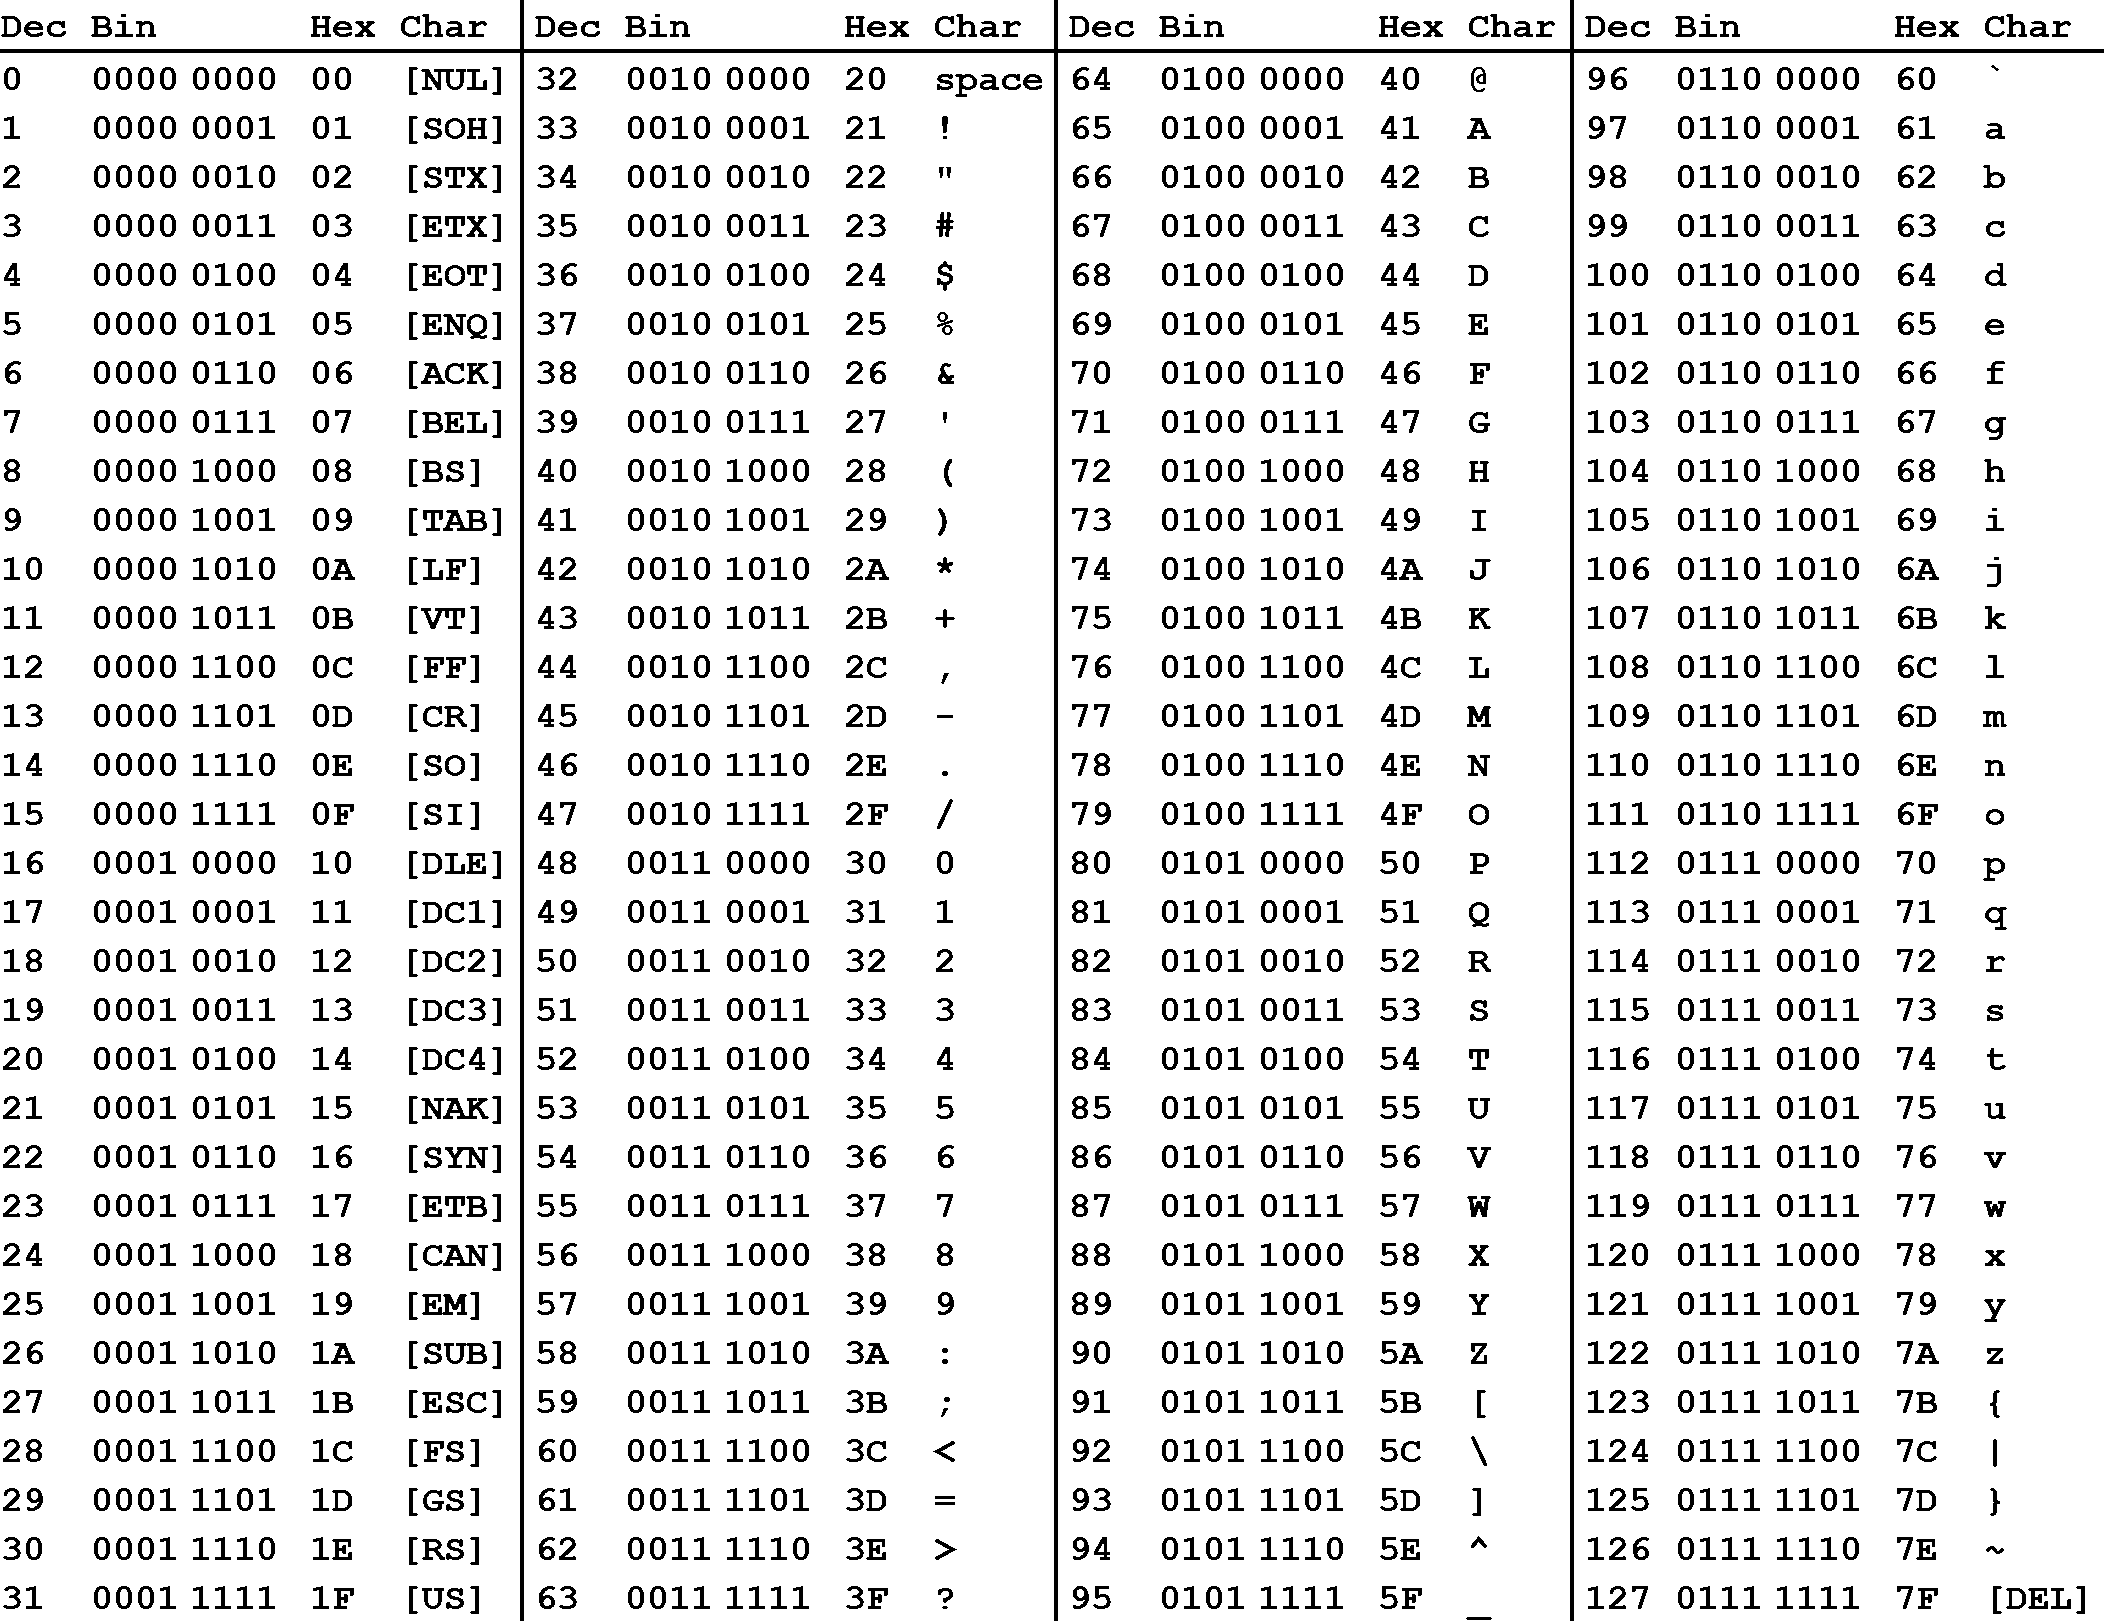
\includegraphics[width=\textwidth]{ascii.png}
    \caption{Bytes als ASCII waardes}
    \label{fig:ascii}
\end{figure}

Met een byte kunnen we 8-bits binaire getallen opslaan. Deze kunnen we zoals gezegd als getal beschouwen, of bijvoorbeeld als een enkel karakter zoals een letter of leesteken. Voor getallen is het vrij duidelijk hoe we om kunnen rekenen tussen binaire en "normale" decimale representatie, maar voor karakters zijn afspraken nodig. De bitwaarde 01000001 zou voor een uitroepteken kunnen staan, of een letter, of nog heel iets anders. De waarde heeft als karakter zelf geen betekenis, tenzij we die eraan geven. Om ervoor te zorgen dat iedereen dat hetzelfde doet, en je dus tekst uit kunt wisselen tussen computers, zijn hier standaarden voor gemaakt. In figuur~\ref{fig:ascii} zien we de ASCII\sidenote{Inmiddels is de ASCII-standaard achterhaald en is er een codering, Unicode, die met meerdere bytes alle gebruikte karakters kan opslaan, in elke taal. Hier zitten zelfs uitgestorven schriften zoals Runen in, wiskundige en andere symbolen, en emoticons. Qua idee werkt dit hetzelfde als de tabel die we hier zien, maar op veel grotere schaal.} tabel, die met 7-bits (1 bit is ongebruikt) alle latijnse hoofd-/kleine letters, cijfers, leestekens en nog wat onzichtbare karakters kan opslaan. In dit geval staat de waarde 01000001 dus voor de hoofdletter \emph{A}.

\subsection{Pixels in plaatjes}
Een andere manier waarop we een byte kunnen interpreteren is als een pixel. Afhankelijk van de kleurdiepte kan een byte staan voor een hele pixel (er zijn dan 256 mogelijke kleuren) of bijvoorbeeld een enkel kleurkanaal (rood/groen/blauw) van een pixel (met $256 \times 256 \times 256 \approx 16M$ mogelijke kleuren). Aan de andere kant van het spectrum kan een afbeelding ook zwart-wit of greyscale zijn, waarbij respectievelijk 8 pixels in byte passen, of de 256 waardes van een byte een gradient van zwart (0) naar wit (255) vormen.

\begin{figure}[ht]
    \centering
    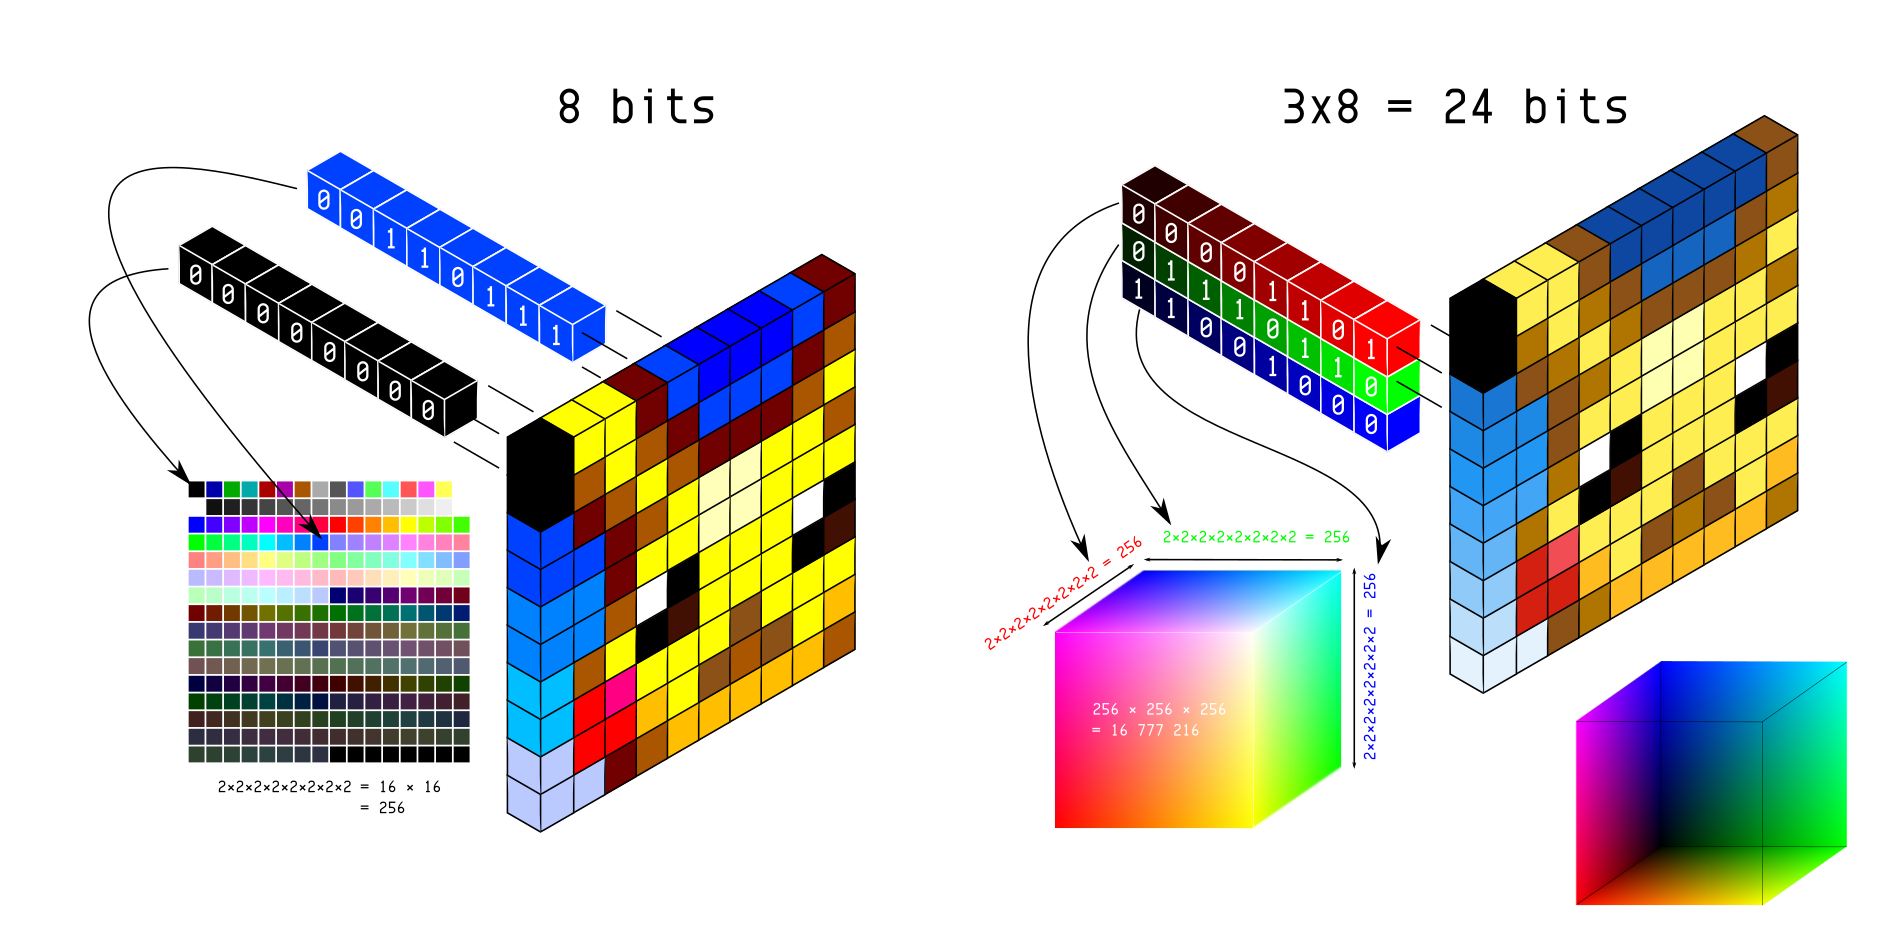
\includegraphics[width=\textwidth]{pixels.png}
    \caption{Bytes als pixeldata}
    \label{fig:pixel}
\end{figure}

\subsection{Arrays en Strings}
Voor karakters en pixels geldt dat deze doorgaans op zichzelf niet zoveel waarde hebben, maar meestal in een reeks gebruikt worden. In algemene zin hebben we het bij zo'n reeks over een \emph{array}, in het geval van karakters gebruiken we \emph{string} om eigenlijk \enquote{array van karakters} te zeggen. Voor de computer is een array simpelweg een reeks waardes van hetzeflde type en hetzelfde geheugen-footprint. Deze worden in het geheugen ook achter elkaar opgeslagen. Een array heeft in principe een vaste grootte (vast aantal elementen en vast formaat per element), om dynamsiche reeksen op te slaan is een data-structuur met heap-opslag noodzakelijk.

\subsection{Data-structuren en Objecten}
In veel gevallen is het nodig om verschillende typen data te combineren tot een enkele logische eenheid. Dit is het geval bij object-geori\"enteerd (OO) programmeren\sidenote{Bij OO wordt code en gerelateerde data als het ware samen verpakt. Voor de computer is er nog steeds een code/data-scheiding, maar voor de programmeur is deze weggemoffeld.}, maar ook zonder OO zullen we te maken hebben met data-eenheden die bijvoorbeeld een tekst-label en getallen (co\"ordinaten) bevatten. Deze datastructuren hebben een vast format, en dit vertaalt zich naar een aaneengesloten\sidenote{Hier zit een kleine versimpeling: onderdelen die kleiner zijn dan de adresseringseenheid (doorgaans 32 of 64 bit) worden met padding tot dat formaat opgevuld. Deze padding kost wel geheugenruimte, maar wordt niet gebruikt. Een enkel \texttt{char} veroorzaakt bijvoorbeeld padding als deze tussen twee 32-bits getallen staat. Twee \texttt{char}s naast elkaar leveren doorgaans maar \'e\'en keer padding op. De preciese regels zijn platform- en compilerafhankelijk.} blok geheugen waarvan de computer weet waar elk onderdeel begint en eindigt. De volgorde in het geheugen wordt bepaald door de volgorde waarin de onderdelen in de programma-code worden aangeboden.


\part{Coding Skills}
\chapter{Linux}\label{ch:linux}

Als ICT-er, en zeker als AI-specialist, zul je te maken krijgen met verschillende computersystemen en hiermee moeten kunnen werken. Voor cloud-servers specifiek is het waarschijnlijk dat je te maken krijgt met een niet-grafische Linux-omgeving. In dit hoofdstuk wordt gekeken naar Bash, de standaard login-shell voor Linux.

\section{Historie}\label{historie}

Linux is een afstammeling van de Unix traditie van besturingssystemen, die teruggaat tot Multics dat in de jaren 60 als time sharing OS voor de Multics GE-645 werd ontwikkeld door MIT, AT\&T Bell Labs en General Electric. Zoals te zien waren computers toen nog grote gedrochten, en was van de personal computer nog geen sprake. Een mainframe, zoals dit type computer heette, werd door hele bedrijven of afdelingen gedeeld. Programmeurs schreven code, waarna ze moesten wachten op hun beurt om de code te draaien. Als er een fout in zat, kon de programmeur opnieuw beginnen en een nieuwe beurt afwachten. Later werd het langzaam mogelijk met meerdere terminals (werkstations) de computer tegelijk te gebruiken. In deze context werd de grondslag voor Unix gelegd.

  \begin{marginfigure}
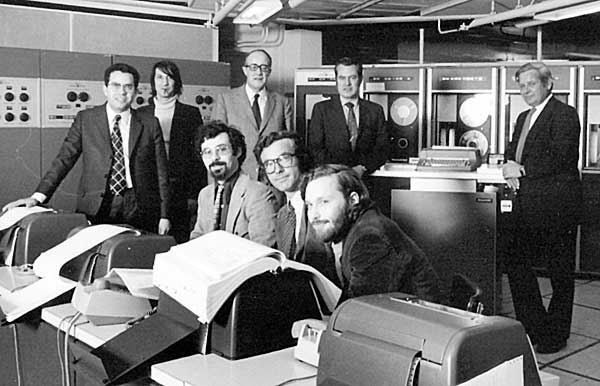
\includegraphics[width=0.8\textwidth]{ge645.jpg}\\
    GE-645 Mainframe {\scriptsize\emph (Image by Wikipedia)}\\[3mm]
  \end{marginfigure}

De ontwikkeling van Multics schoot niet op, waardoor Bell Labs besloot haar onderzoekers terug te trekken. Een deel daarvan, met name Ken Thompson, Dennis Ritchie en Brian Kernighan, ging bij Bell Labs verder met hun werk, maar op een kleinere schaal. Het resultaat hiervan is Unix. Unix had een eigen filosofie, waarbij alles als een file gezien werd (ook, bijvoorbeeld, devices). Hierdoor werd het makkelijker programma's aan elkaar te koppelen, met ``bestanden'' als koppelstukken. Dit leidde tot een filosofie van kleine, algemene programma's die oneindig in te zetten en te combineren waren. Dennis Ritchie vatte de filosofie samen als \emph{``What we wanted to preserve was not just a good environment in which to do programming, but a system around which a fellowship could form. We knew from experience that the essence of communal computing, as supplied by remote-access, time-shared machines, is not just to type programs into a terminal instead of a keypunch, but to encourage close communication.''}

  \begin{marginfigure}
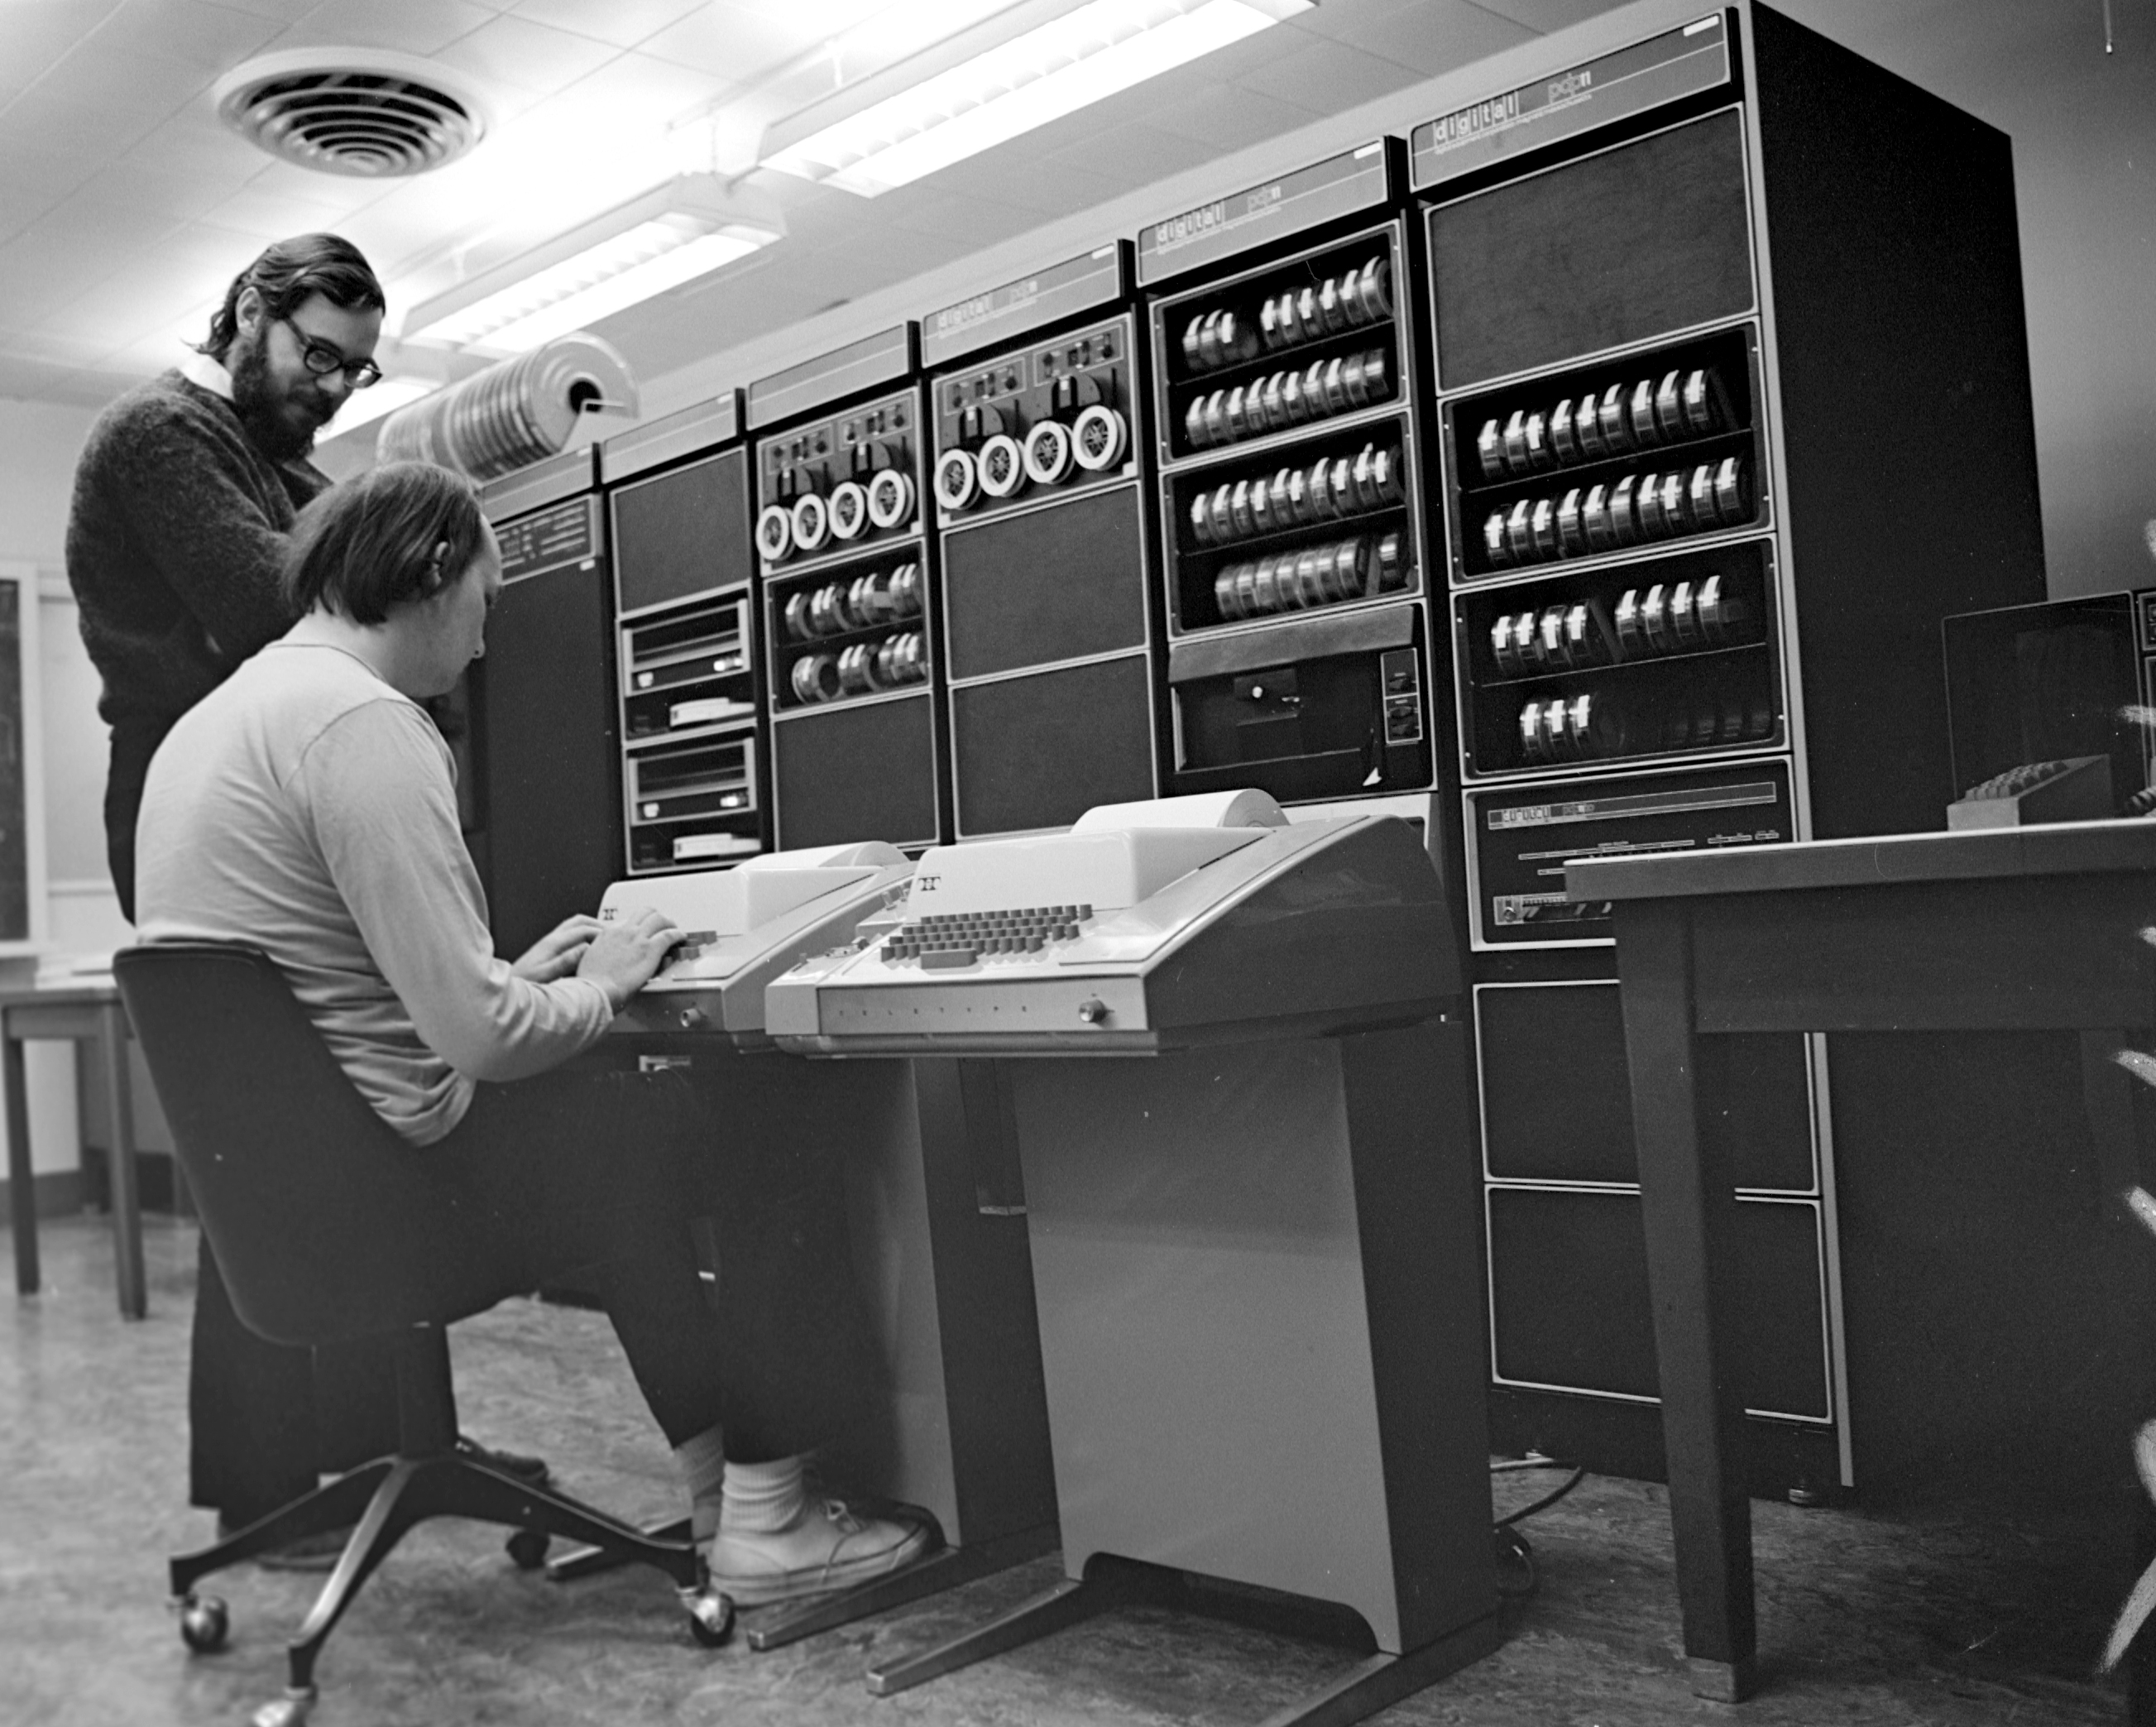
\includegraphics[width=0.8\textwidth]{thompson_ritchie.jpg}\\
    Thompson en Ritchie {\scriptsize\emph (Image by Wikipedia)}\\[3mm]
  \end{marginfigure}

De volgende stap richting Linux was Minix, geschreven door Andrew S. Tanenbaum. Minix was een erg versimpelde Unix afgeleidde die vooral educatief bedoeld was. De hele source-code, gecombineerd met de theorie waarop deze gebaseerd was, was als boek te koop (in het Turing Lab ligt een exemplaar). Hoewel de source-code beschikbaar was, was het niet toegestaan deze te verbeteren of te verspreiden. Daarnaast was de code vanuit educatief perspectief erg goed, maar praktisch gezien vooral al snel verouderd.

\subsection{Linux}\label{linux}

Linus Torvalds was een student informatica bij de Universiteit van Helsinki. Gebaseerd op het boek van Tanenbaum begon hij in 1991 met zijn eigen OS Kernel. Toen dit een beetje vorm begon te krijgen heeft hij dit \href{https://www.cs.cmu.edu/~awb/linux.history.html}{op usenet beschikbaar gesteld} voor wie er iets mee wilde.

  \begin{marginfigure}
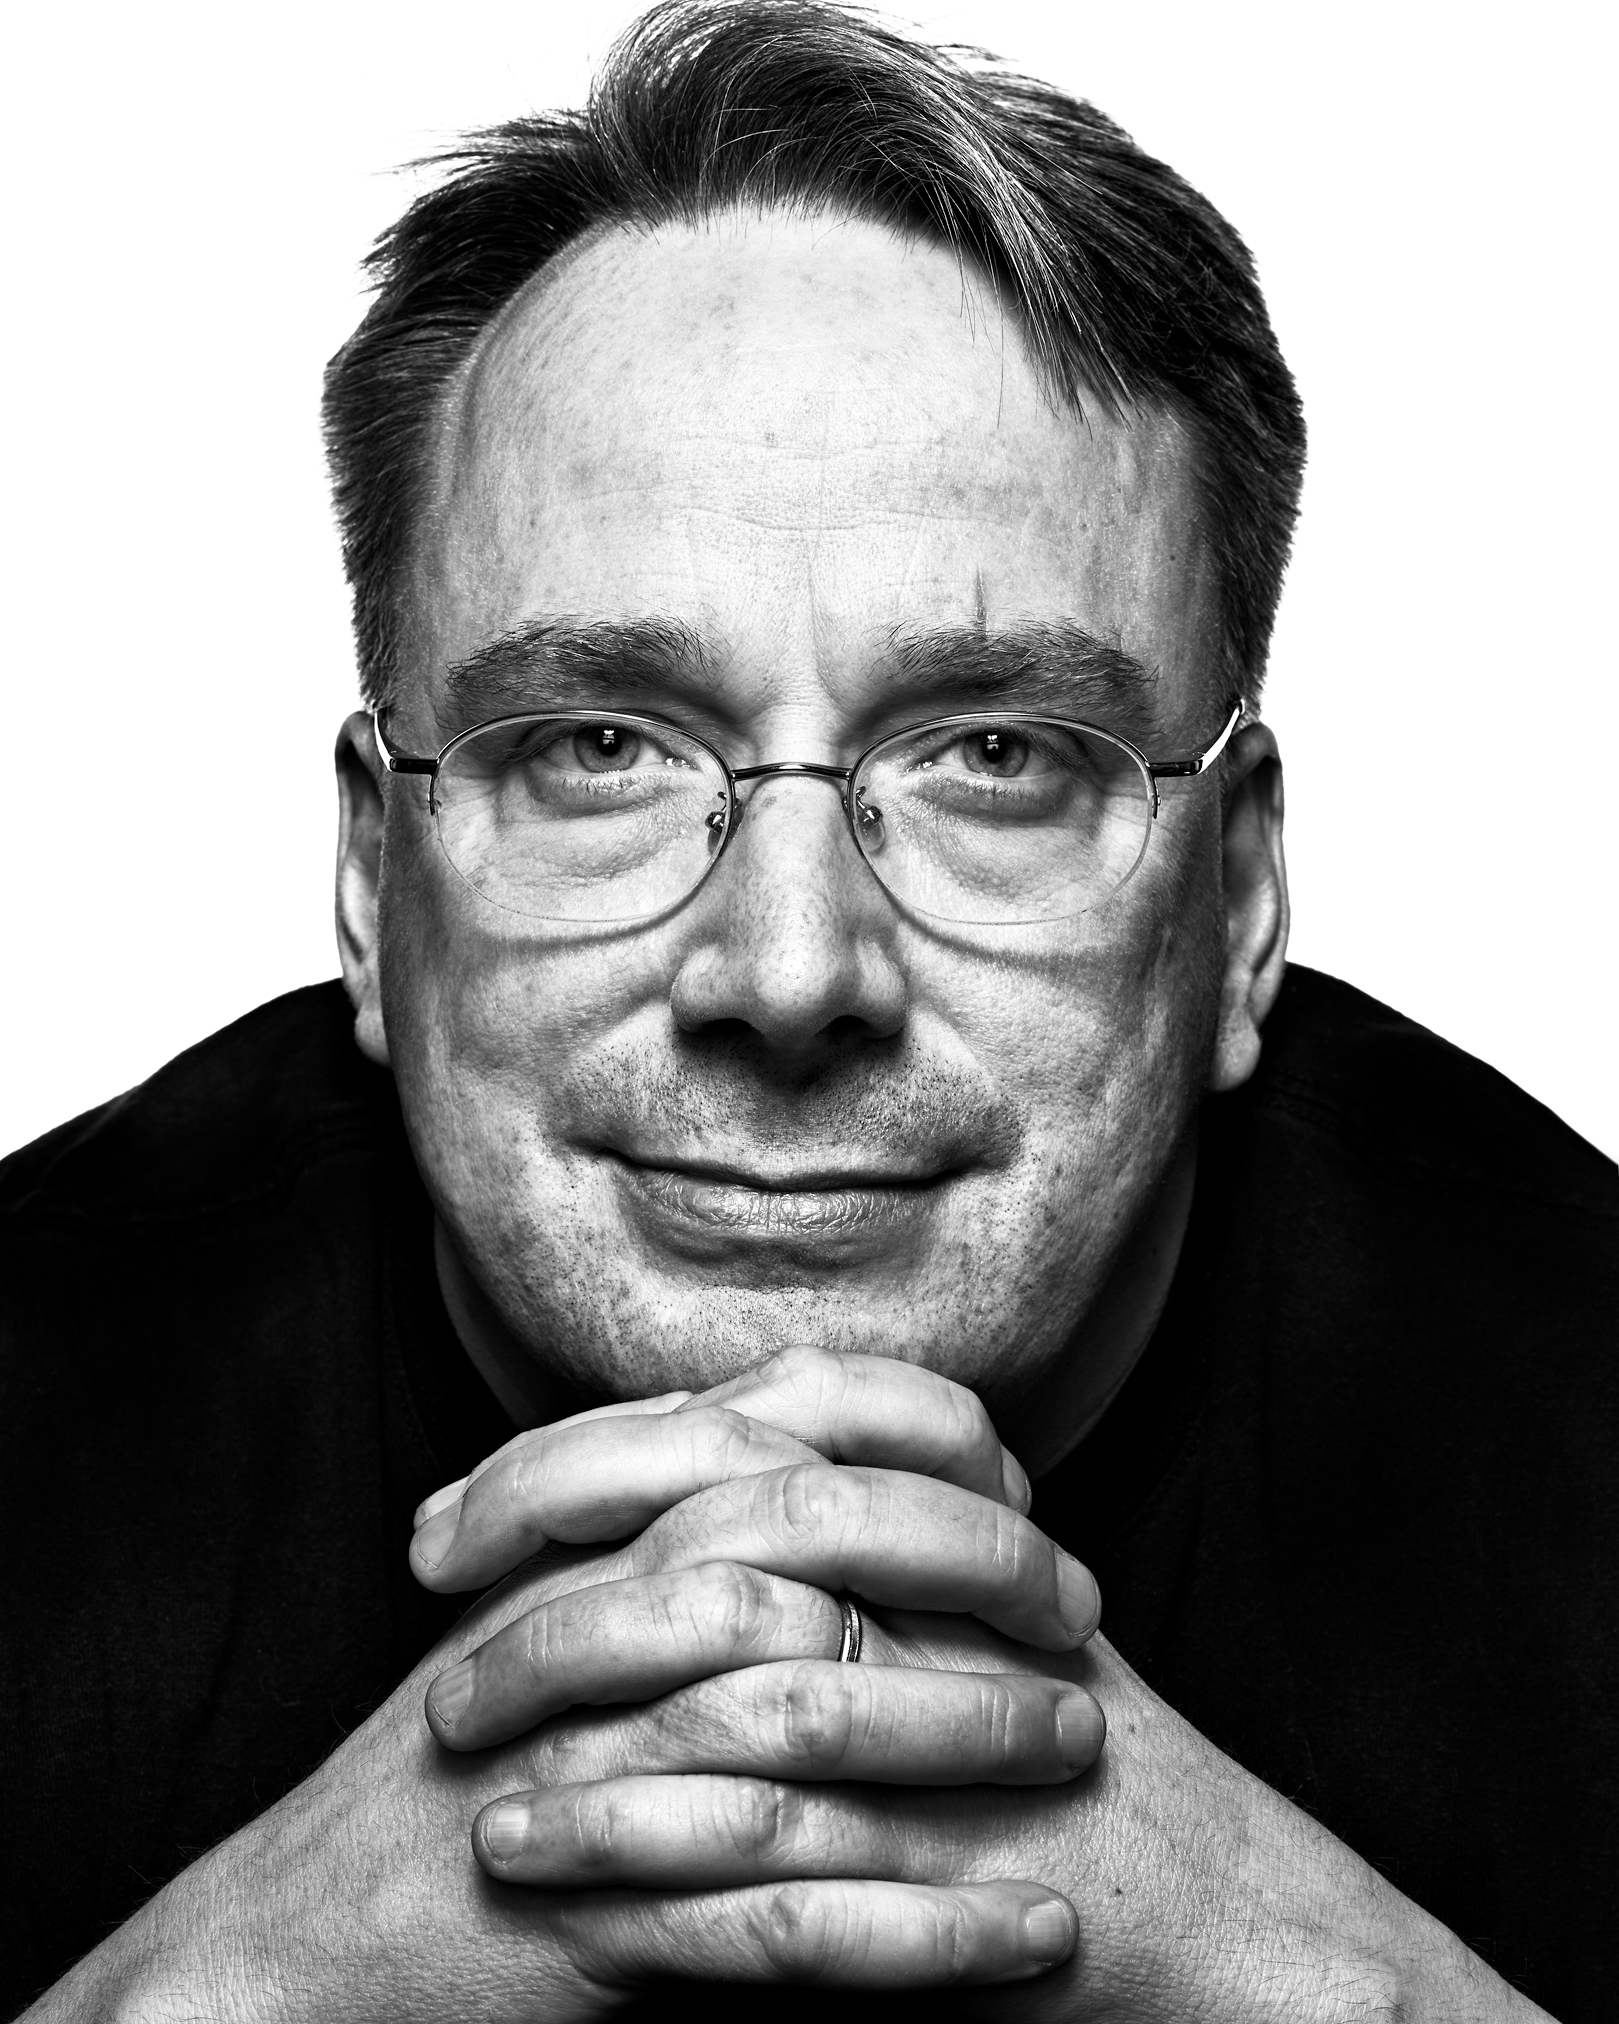
\includegraphics[width=0.6\textwidth]{linus.jpg}\\
    Linus Torvalds {\scriptsize\emph (Image by Wikipedia)}\\[3mm]
  \end{marginfigure}

Ondertussen was Richard M. Stallman bezig met een eigen gratis (en vooral: open source) Unix vervanger: \href{https://www.gnu.org/}{GNU} (GNU's Not Unix). Dit was grotendeels compleet, alleen de kernel die hij ontwikkelde wilde geen kritieke massa krijgen. Omdat Linus bij zijn ontwikkeling gebruik had gemaakt van het werk dat voor GNU verzet was, was het een logische stap de twee projecten te combineren tot GNU/Linux. Hoewel we meestal gewoon Linux zeggen, is GNU/Linux de geprefereerde naam voor het hele OS.

  \begin{marginfigure}
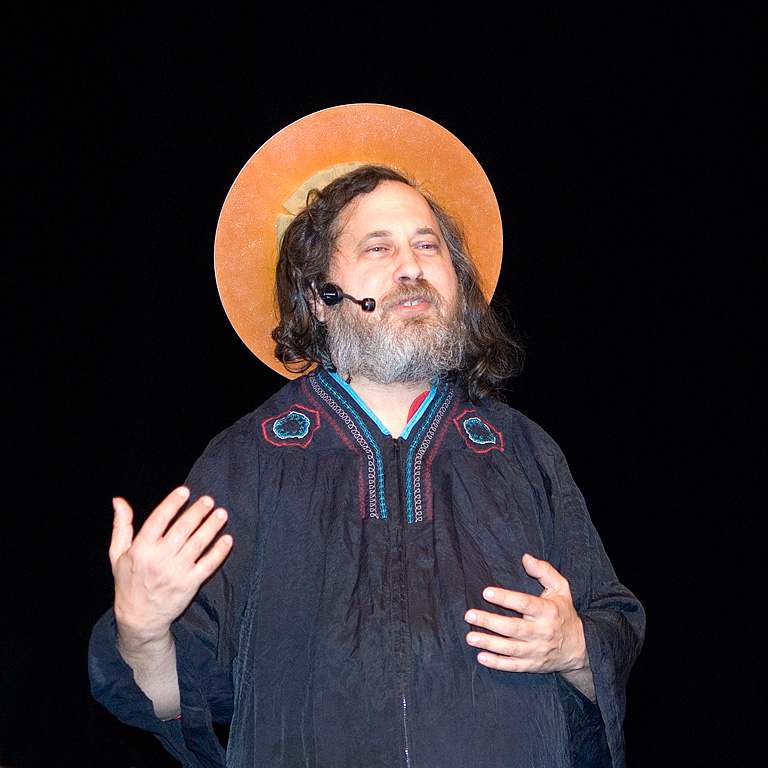
\includegraphics[width=0.6\textwidth]{rms.jpg}\\
    Richard Stallman {\scriptsize\emph (Image by Wikipedia)}\\[3mm]
  \end{marginfigure}

\subsection{Open Source}\label{open-source}

GNU en Linux vallen beide onder de \href{https://www.gnu.org/copyleft/gpl.html}{GNU General Public License}, een open source licentie. Dit houdt in dat de source code vrij beschikbaar is, mag worden aangepast en mag worden doorgegeven. Er is een grote diversiteit aan open source licenties in gebruik, en nog meer licenties die ruwweg dezelfde ideeën bevatten maar net niet aan de eisen voldoen om ``open source'' te mogen heten. Een deel van de open source licenties, waaronder de GPL, heeft een clausule die stelt dat hoewel je de code mag aanpassen, dat de resultaten daarvan ook onder dezelfde licentie moeten vallen. Andere open source licenties hebben deze eis niet. Merk op dat er geen verbod is op het verkopen van GPL software (of diensten daaromheen) of andere commerciële toepassingen (al zijn er licenties die dat wel hebben), zolang de source maar vrijelijk beschikbaar blijft. Later in deze les zullen we een aantal commerciële / betaalde toepassingen van Linux tegenkomen.

\section{De command-line}

In deze sectie maken we kennis met Bash, de meest gangbare shell voor Linux. Ook komen we een diversiteit aan programma's tegen die we vanaf de command line kunnen gebruiken. Het is in Bash niet altijd duidelijk welk commando een ``built-in'' functie van Bash is, en welk command een programma is: omdat Bash gebruikt wordt om programma's aan elkaar te knopen is deze grens behoorlijk vervaagd. Deze kennis is meestal ook niet nodig om Bash te gebruiken, maar wel iets om in het achterhoofd te houden.

\subsection{Je weg vinden op de command-line}\label{je-weg-vinden-op-de-command-line}

Als je een nieuwe terminal start\sidenote{of via bijvoorbeeld SSH een verbinding maakt}, heeft je shell standaard een working directory: het punt op het filesysteem waar je je bevindt. Bestanden die je maakt worden in deze map gezet, en bestanden die je zoekt kunnen relatief vanaf deze map benaderd worden. Standaard zul je beginnen in je \emph{home} directory, de map die je als gebruiker zelf beheert en waar je eigen bestanden (en instellingen) te vinden zijn. Het commando \texttt{cd} (change directory) wordt gebruikt om van map te wisselen, en \texttt{pwd} (present working directory) vertelt waar je je nu bevindt. Met \texttt{ls} (list) kun je de inhoud van de huidige map te zien krijgen. Een aantal paden zijn belangrijk om te weten: de bovenste directory, de root directory, wordt met een \texttt{/} (slash) aangeduid. Vanaf hier worden directory-namen door een \texttt{/} gescheiden om een pad uit te drukken. De home directory van de gebruiker \texttt{linus} bevindt zich bijvoorbeeld op \texttt{/home/linus} (de map \texttt{linus}, binnen de map \texttt{home}, binnen de root). \texttt{\textasciitilde} wordt gebruikt als synoniem voor de home directory van de huidige gebruiker. Voor linus is \texttt{cd\ \textasciitilde} dus hetzelfde als \texttt{cd\ /home/linus}. \texttt{.} verwijst naar de huidige map: \texttt{cd\ .} doet niets. Dit kan voor nu een beetje overbodig lijken, maar later zullen we zien hoe de \texttt{.} soms korter is dan de alternatieven. Daarnaast hebben we \texttt{..}, die naar de parent van de huidige directory verwijst. Vanaf Linus's home zal \texttt{cd\ ..} dus naar \texttt{/home} verwijzen. Deze kun je ook middenin een pad gebruiken, de map omhoog wordt dan gerekend vanaf waar in het pad deze wordt gebruikt. \texttt{cd\ /home/linus/Documents/../Music} is bijvoorbeeld hetzelfde als \texttt{cd\ /home/linus/Music}. \texttt{cd} zonder argument gaat terug naar de home directory, en \texttt{cd\ -} gaat terug naar de vorige directory.

\begin{bash}
\p cd Documents\\
\  \\
\p[\textasciitilde/Documents] pwd\\
/home/linus/Documents\\\\
\  \\
\p[\textasciitilde/Documents] cd ..\\
\  \\
\p cd Folder\\
\  \\
\p[\textasciitilde/Folder] cd ..\\
AnotherFile  File\\
\  \\
\p[\textasciitilde/Folder] cd \asciitilde\\
\  \\
\p cd -\\
/home/linus/Folder
\  \\
\p[\textasciitilde/Folder] cd .\\
\  \\
\p[\textasciitilde/Folder] cd /\\
\  \\
\p[/] ls\\
bin/  boot/  dev/  etc/  home/  media/  mnt/  proc/  root/  run/  sys/  tmp/  usr/  var/\\
\  \\
\p[/] cd\\
\  \\
\p pwd\\
/home/linus\\
\end{bash}

De volgende commando's manipuleren bestanden. Met \texttt{touch} wordt een bestand aangemaakt (als deze nog niet bestond) of wordt de ``laatst aangepast'' datum naar nu gezet. Het bestand wordt gewijzigd, maar er verandert niets aan. Met \texttt{cp} kun je een bestand kopiëren, en met \texttt{mv} kun je het verplaatsen. \texttt{rm} verwijdert een bestand.

\begin{bash}
\p ls\\
AnotherFile  File\\
\\
\p touch File3\\
\\
\p ls\\
AnotherFile  File  File3\\
\\
\p cp File File2\\
\\
\p ls\\
AnotherFile  File  File2  File3\\
\\
\p mv AnotherFile File1\\
\\
\p ls\\
File  File1  File2  File3\\
\\
\p rm File3\\
\\
\p ls\\
File  File1  File2\\
\end{bash}

De meeste commando's voor bestanden werken niet direct op directories. \texttt{mv} mag, maar \texttt{cp} en \texttt{rm} werken niet. Voor het verwijderen van een \emph{lege} map wordt \texttt{rmdir} gebruikt, maar dit mag niet als er een bestand in de map zit. Dit is omdat Linux je wil beschermen geen verkeerde handeling uit te voeren: als je aangeeft dat je een bestand wil verwijderen, maar je geeft een map op, dan is de kans groot dat je de verkeerde naam hebt meegegeven. Als je toch een map (met alle inhoud) wilt kopiëren of verwijderen, kun je \texttt{cp\ -r} en \texttt{rm\ -r} gebruiken. De toevoeging \texttt{-r} staat voor \emph{recursief} (dat betekent in dit geval: met alles wat eronder hangt). Gebruik bijvoorbeeld \texttt{rm\ -r\ Music} als je de map Music met alle inhoud wil verwijderen. \texttt{-r} is het eerste voorbeeld van een flag.

\begin{bash}
\p[~/Folder] ls\\
File  File1  File2\\
\\
\p[~/Folder] mkdir Subfolder\\
\\
\p[~/Folder] touch Subfolder/File\\
\\
\p[~/Folder] mkdir EmptyFolder\\
\\
\p[~/Folder] ls\\
EmptyFolder/  File  File1  File2  Subfolder/\\
\\
\p[~/Folder] mkdir EmptyFolder2\\
\\
\p[~/Folder] ls\\
EmptyFolder/  EmptyFolder2/  File  File1  File2  Subfolder/\\
\\
\p[~/Folder] rmdir EmptyFolder\\
\\
\p[~/Folder] rmdir Subfolder\\
rmdir: failed to remove 'Subfolder/': Directory not empty\\
\\
\p[~/Folder] cp Subfolder Backup\\
cp: -r not specified; omitting directory 'Subfolder'\\
\\
\p[~/Folder] cp -r Subfolder Backup\\
\\
\p[~/Folder] ls\\
Backup/  EmptyFolder2/  File  File1  File2  Subfolder/\\
\\
\p[~/Folder] rm -r Subfolder\\
\\
\p[~/Folder] rm -r EmptyFolder2\\
\\
\p[~/Folder] ls\\
Backup/  File  File1  File2\\
\end{bash}

\subsection{Flags / Command Line Arguments}\label{flags-command-line-arguments}

De meeste commando's accepteren command line argumenten. Allereerst zijn er verplichte argumenten. Waar \texttt{pwd} bijvoorbeeld geen argumenten nodig heeft, heeft \texttt{touch} enkel zin als meegegeven wordt welk bestand gemaakt of geüpdatet moet worden. \texttt{cp} heeft zelfs twee argumenten nodig: een bron en een doel. Soms kan een commando een optioneel pad meekrijgen: \texttt{ls} werkt in de huidige working directory, \texttt{ls\ /home} leest de inhoud van \texttt{/home}. Al deze argumenten zijn positie-bepaald. Het eerste argument bij \texttt{cp} is altijd de bron, de tweede het doel. Naast deze positiegebonden argumenten hebben we ook flags, die met één of twee streepjes (dashes) kunnen beginnen. Flags komen doorgaans overeen met booleaanse waardes: wel of niet. Als de flag met één dash begint, dan is het doorgaans een enkele letter, en kun je deze combineren. \texttt{-r\ -f} is hetzelfde als \texttt{-rf}; het maakt niet uit of je \texttt{rm\ -r\ -f\ Music} gebruikt of het kortere \texttt{rm\ -rf\ Music}. Ook de volgorde maakt meestal niet uit. Flags met een dubbele dash bestaan uit meerdere letters en zijn niet samen te voegen. Tot slot kunnen deze flags soms een argument erbij nemen. Bij enkele letters volgt het argument meestal na een (optionele) spatie, bij de dubbele dash wordt meestal een \texttt{=} gebruikt om de waarde van de flag te scheiden.

\begin{bash}
\p[~/Folder] ls\\
File  File1  File2  Folder1/  Folder2/ Folder3/\\
\\
\p[~/Folder] rm -r Folder1    \# Recursive om directory te deleten\\
\\
\p[~/Folder] rm -f File2      \# Force remove\\
\\
\p[~/Folder] rm -r -f Folder2 \# Force recursive remove\\
\\
\p[~/Folder] rm -rf Folder3   \# Zelfde als -r -f\\
\\
\p[~/Folder] rm --force File1 \# Zelfde als -f\\
\\
\p[~/Folder] ls\\
File\\
\end{bash}

Sommige commando's hebben erg veel opties om de gewenste functionaliteit te selecteren. De meeste commando's hebben een \texttt{-h} en/of \texttt{-\/-help} optie om wat tips te geven over het gebruik. Voor het hele verhaal kun je \texttt{man} gebruiken, oftewel de manual.

\begin{bash}
\p[~] rm --help\\
\# Print een (relatief) korte handleiding\\
\\
\p[~] man rm\\
\# Scroll door de uitgebreide handleiding\\
\end{bash}

\subsection{IO en Pipes}\label{io-en-pipes}

Om een tree te krijgen van de inhoud van een map en alle submappen kun je het commando \texttt{find} gebruiken. Dit geeft echter vrij veel uitvoer, het zou fijn zijn als we hier hapklare brokken van konden maken. Het commando \texttt{less} kan gebruikt worden om een bestand te openen en er doorheen te kunnen scrollen. Kunnen we dit gebruiken om de uitvoer van \texttt{find} te pagineren? In Linux kun je twee commando's aan elkaar koppelen: uitvoer van het ene programma wordt als invoer voor het tweede gebruikt. Hiervoor gebruiken we het \texttt{\textbar{}} symbool: de pipe. Denk aan een pijpleiding die de commando's met elkaar verbindt.

\begin{bash}
\p[~] find /home/linus\\
\# Print de hele mappenstructuur; veel output\\
\\
\p[~] less file\\
\# Lees een bestand door er doorheen te scrollen\\
\\
\p[~] find /home/linus | less\\
\# Combineer de tools: scroll door de uitvoer van find\\
\end{bash}


\newthought{Pipes zijn een fundamenteel deel van de Unix filosofie} om eenvoudige programma's te combineren voor complex gedrag. Het sturen van de uitvoer noemen we het \emph{redirecten} van \texttt{STDOUT} (standard out), en het lezen van de invoer is het \emph{redirecten} van \texttt{STDIN} (standard in). Dit hoeft niet met een pipe te gebeuren, maar kan ook van/naar een bestand. \texttt{STDOUT} is een file descriptor (nummer 1) die in ieder proces aanwezig is, en die gebruikt wordt om alles naartoe te schrijven dat het programma uitvoert (denk aan \texttt{print}s). \texttt{STDIN} is ook een file descriptor (nummer 0), maar deze wordt gelezen voor invoer. Normaal is dit de gebruikersinvoer vanaf de command line, maar dit kan ook prima een bestand of pipe zijn. Daarnaast is er vaak een derde file descriptor, \texttt{STDERR} (standard error, nummer 2), voor foutmeldingen (ook dit is standaard de command line, maar het is hiermee dus mogelijk te splitsen tussen uitvoer en excepties). Het gebruik van file descriptors voor de invoer/uitvoer is weer een voorbeeld van de UNIX-filosofie dat alles een bestand is. Een descriptor is de datastructuur die UNIX intern gebruikt om iets te kunnen benaderen; een file descriptor verwijst dus naar een bestand (en hoe dit gelezen/geschreven kan worden). Waar \texttt{STDIN} en \texttt{STDOUT} precies aan verbonden zijn, is te vinden in de environment informatie die bij een proces hoort. Standaard zijn dit voor processen die je in de shell start de invoer en de uitvoer van de terminal, en als je een child process start worden deze overgeërfd. Tijdens executie van het proces kunnen deze descriptors altijd worden gesloten of ergens anders aan verbonden worden. Bij processen die door de kernel gestart worden, zoals \texttt{init} is de \texttt{STDOUT} doorgaans aan het kernel log gekoppeld. \texttt{STDIN} kan aan een buffer of (als het proces geen input verwacht) aan een dummy file gekoppeld zijn: een lege file descriptor die niet aan een daadwerkelijk bestand op de schijf gekoppeld is.

\begin{figure}[ht]
    \centering
    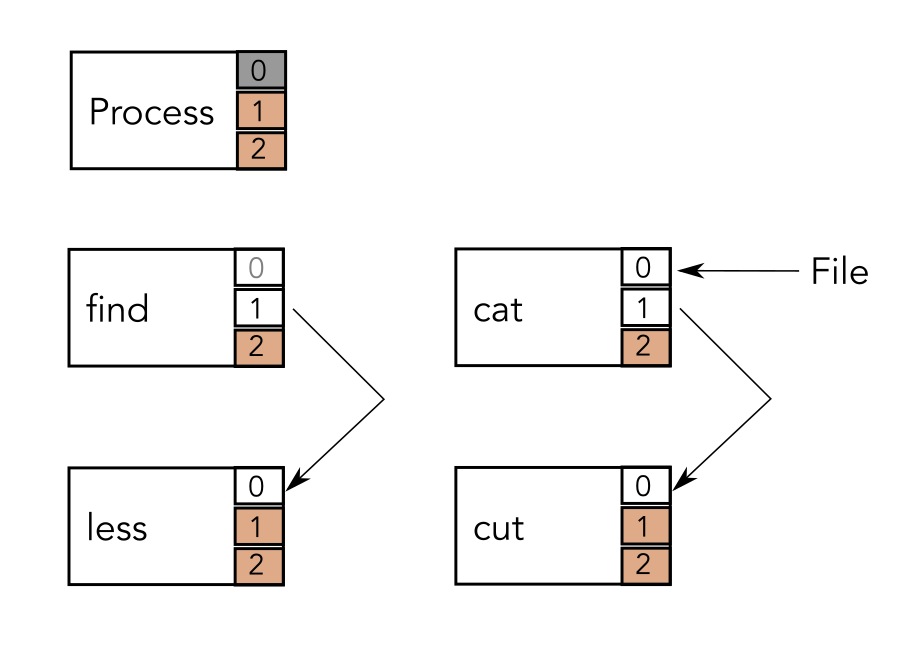
\includegraphics[width=\textwidth]{io.png}
    \caption{File Descriptors van een Proces}
    \label{fig:process-io}
\end{figure}

Net als dat we vanaf de shell twee commando's aan elkaar kunnen pipen, kunnen we ook een file descriptor meegeven om als \texttt{STDIN}, \texttt{STDOUT} of \texttt{STDERR} te gebruiken. Dit kan respectievelijk met \texttt{\textless{}}, \texttt{\textgreater{}} en \texttt{2\textgreater{}}. Je kunt bijvoorbeeld \texttt{find\ /home/linus\ \textgreater{}\ filetree} gebruiken om de uitvoer van \texttt{find\ /home/linus} in het bestand \texttt{filetree} te schrijven. Bij \texttt{find\ /home/linus\ 2\textgreater{}\ errors.log} wordt niet de uitvoer verbonden, maar eventuele foutmeldingen via \texttt{STDERR}. Als het bestand waarnaar je wilt uitvoeren al bestaat, wordt het als je \texttt{\textgreater{}} gebruikt overschreven, maar je kunt, \texttt{\textgreater{}\textgreater{}} en \texttt{2\textgreater{}\textgreater{}} gebruiken om in plaats daarvan achteraan het bestand toe te voegen. Tot slot kun je \texttt{\textless{}\textless{}\ MARKER} of \texttt{\textless{}\textless{}-\ MARKER} (een zogenaamde ``heredoc'') gebruiken om \texttt{STDIN} vanaf de command line mee te geven, tot aan de eerste regel met enkel \texttt{MARKER}. Dit maakt het makkelijk meerdere regels tekst mee te geven. De toegevoegde waarde van de \texttt{-} is dat deze een tab aan het begin van een regel negeert en mogelijk leesbaarder is. Op zichzelf wordt \texttt{\textless{}} niet zo veel gebruikt, omdat de meeste programma's standaard een meegegeven bestandsnaam als \texttt{STDIN} interpreteren (dus \texttt{less\ \textless{}\ file} is hetzelfde als \texttt{less\ file}), maar bij sommige programma's kan dit nodig zijn. Een voorbeeld is \texttt{psql}, een database waarbij je een bestand met instructies mee kan geven met \texttt{psql\ databasename\ \textless{}\ sqlfile}. Als je \texttt{\textless{}} niet gebruikt en vanaf de command line invoert kun je \texttt{Control-d} gebruiken om je invoer te beëindigen, in plaats van de explicete \texttt{MARKER} die je bij \texttt{\textless{}\textless{}} gebruikt. \texttt{wc} staat trouwens voor \emph{word count}, waarbij \texttt{wc\ -l} het aantal regels telt, en \texttt{wc\ -c} het aantal karakters.

\begin{bash}
\p[~] find /home/linus > filetree 2> errors.log\\
\# Geen output; alles staat in bestanden filetree en errorslog\\
\\
\p[~] wc -l filetree >\!> filetree\\
\# Het totaal aantal regels in filetree wordt onderaan filetree toegevoegd\\
\\
\p[~] wc -c <\!< EOF\\
> Lorem Ipsum\\
> Dolor Sit Amet\\
> EOF\\
27\\
\\
\p[~] psql databasename < sqlfile\\
\# Laadt een database uit een file\\
\end{bash}

\subsection{Meer Commando's met Pipes}\label{meer-commandos-met-pipes}

Nu we het bestaan van pipes kennen, zijn hier nog wat commando's die op zichzelf niet altijd even zinvol zijn, maar als deel van een pipeline goed werken. Om uit bestand (of uitvoer) regels te filteren die een bepaalde string bevatten kun je \texttt{grep} gebruiken. \texttt{sort} geeft de invoer gesorteerd terug, en \texttt{cut} snijdt per regel een substring uit. In het onderste voorbeeld wordt \texttt{ls\ -l} gebruikt (een directory listing met uitgebreide info). We gebruiken \texttt{cut\ -c14-} om karakter 14 tot eind te bewaren, waardoor de eigenaar van het bestand vooraan komt te staan. Met \texttt{sort} kunnen we hierop sorteren.

\begin{bash}
\p[~/Folder] ls -la\\
total 0\\
drwxr-xr-x 1 linus users   44 Jan 28 10:10 .\\
drwx------ 1 linus users 6142 Jan 28 10:05 ..\\
-rw-r--r-- 1 root  users    0 Jan 28 09:46 File\\
-rw-r--r-- 1 linus users    0 Jan 28 10:08 File2\\
-rw-r--r-- 1 linus users    0 Jan 28 10:08 File2025\\
-rw-r--r-- 1 linus users    0 Jan 28 10:08 File3\\
\\
\p[~/Folder] ls -la | grep 2025\\
-rw-r--r-- 1 linus users 0 Jan 28 10:08 File2025\\
\\
\p[~/Folder] ls -la | cut -c14- | sort\\
\\
linus users    0 Jan 28 10:08 File2\\
linus users    0 Jan 28 10:08 File2025\\
linus users    0 Jan 28 10:08 File3\\
linus users   44 Jan 28 10:10 .\\
linus users 6142 Jan 28 10:05 ..\\
root  users    0 Jan 28 09:46 File\\
\end{bash}

\subsection{Pipelines en Command-lists}\label{pipelines-en-command-lists}

Meerdere commands gescheiden door pipes vormen samen een pipeline. De commando's worden parallel uitgevoerd. Je kunt ook meerdere commands na elkaar uit laten voeren, dit kan met de puntkomma en wordt een command-list genoemd. Het is zelfs mogelijk meerdere pipelines in een command list te zetten.

\begin{bash}
\p[~] foo | bar\\
\# De uitvoer van foo gaat naar bar\\
\\
\p[~] foo ; bar\\
\# bar wordt na foo uitgevoerd\\
\\
\p[~] foo | bar ; baz | quux\\
\# Eerst worden foo en bar uitgevoerd, waarbij de uitvoer van foo naar bar gaat\\
\# Als dit klaar is worden baz en quux gestart, en gaat de uitvoer van baz naar quux\\
\end{bash}

Commands in een command list worden na elkaar uitgevoerd, ongeacht of er ergens iets mis gaat. Soms wil je het tweede command enkel uitvoeren als het eerste command geslaagd is, of juist alleen als er een fout is geweest. Zoals we weten heeft ieder command een exit status, \texttt{0} voor succes of iets anders voor een fout. Door \texttt{\&\&} tussen commands te zetten, in plaats van \texttt{;} wordt het tweede commando alleen uitgevoerd als het eerste geslaagd is. De dubbele pipe \texttt{\textbar{}\textbar{}} werkt precies andersom: het tweede command wordt alleen uitgevoerd als de eerste mislukte. We noemen deze operators \emph{en} en \emph{of}. ``Doe a en b'' kan alleen maar als \emph{a} gelukt is, zo niet zal de shell het meteen opgeven. ``Doe a of b'' levert de shell een alternatief, probeer eerst \emph{a}, en als dat niet lukt, doe dan \emph{b}.

\begin{bash}
\p[~] foo || bar\\
\# bar wordt uitgevoerd als foo faalt\\
\\
\p[~] foo && bar\\
\# bar wordt uitgevoerd als foo gelukt is\\
\end{bash}

\subsection{Procesmanagement}\label{procesmanagement}

Als je wilt weten welke processen er op dit moment actief zijn kun je het commando \texttt{ps} gebruiken. Normaal geeft dit alleen een lijst met je eigen processen in terminals, maar met \texttt{ps\ -A} krijg je alle processen te zien. De standaarduitvoer geeft (afhankelijk van je distributie) in ieder geval de PID, terminal en het command. Vaak wordt ook de effectieve tijd die het proces gedraaid heeft meegegeven (effectieve tijd telt alleen de tijd dat het proces daadwerkelijk actief was). Daarnaast heeft \texttt{ps} nog heel veel opties om processen te selecteren en aan te geven welke informatie je wel en niet wil hebben, zie daarvoor de \texttt{man} pagina. \texttt{ps} geeft een eenmalige uitvoer van de processenlijst op dat moment; dit is handig als je dit met andere commands in een pipeline wil combineren. Soms wil je echter een dynamische lijst die zichzelf update, zoals het taakbeheer in Windows. Hier is het commando \texttt{top} voor, of de verbeterde versie \texttt{htop} (meestal niet standaard geïnstalleerd). Tot slot kan je een proces vanaf de command line beëindigen (op voorwaarde dat je zelf de eigenaar van het proces bent). Hiervoor gebruik je \texttt{kill} met de PID van het proces, of \texttt{killall} met de naam van het proces. De laatste heet killall, omdat het goed kan zijn dat je meerdere instanties van dezelfde executable open hebt staan. \texttt{killall\ firefox} sluit bijvoorbeeld alle Firefox vensters, niet een specifieke.

\begin{bash}
\p[~] ps\\
\# geef de processen binnen de huidige shell\\
\\
\p[~] ps -A\\
\# geef alle processen\\
\\
\p[~] top\\
\# interactieve "task manager"\\
\\
\p[~] kill\\
\# stop een proces met een gegeven PID\\
\\
\p[~] killall\\
\# stop elk proces met een gegeven naam\\
\end{bash}

\subsection{Signals}\label{signals}

\texttt{kill} en \texttt{killall} zullen standaard een \texttt{SIGTERM} signaal naar een proces sturen: een vriendelijk doch dringend verzoek om op te houden te bestaan. Dit betekent dat het proces de gelegenheid heeft achter zich op te ruimen, de gebruiker te vragen of zij de wijzigingen op wil slaan, of het verzoek te negeren. Er bestaan echter meerdere signalen die je kan sturen, de belangrijksten staan in de tabel hieronder. Om bijvoorbeeld een \texttt{SIGKILL} signaal te versturen (om een proces direct en \emph{with extreme prejudice} om zeep te helpen) kan dit met \texttt{kill\ -SIGKILL}. \texttt{SIGSTOP} pauzeert een proces, dat met \texttt{SIGCONT} weer hervat kan worden. In de tussentijd is het proces bevroren, en zal het niet gescheduled worden. Een GUI applicatie zal wel een scherm behouden, maar nergens meer op reageren tot het een \texttt{SIGCONT} ontvangt. De tabel met beschikbare signalen is groot, en bevat ook signalen die normaal alleen voor intern gebruik zijn: \texttt{SIGSEGV} wordt bijvoorbeeld door de kernel gestuurd als een proces buiten zijn geheugenruimte opereert (een Segmentation Fault), en \texttt{SIGFPE} wordt onder andere door de CPU gestuurd naar een proces dat door 0 probeert te delen. De hele tabel is in de Linux documentatie of op internet te vinden. De getallen zijn de interne waardes die het OS herkent, de namen zijn enkel om het de gebruiker makkelijker te maken.

\begin{itemize}
  \item \texttt{SIGKILL(9)} Proces beëindigen, kan niet afgevangen worden \\
  \item \texttt{SIGUSR1(10)} User defined, verschilt per programma \\
  \item \texttt{SIGTERM(15)} Standaard signaal, ``sterf, alsjeblieft'' \\
  \item \texttt{SIGCONT(18)} Hervat een gestopt (gepauseerd) proces \\
  \item \texttt{SIGSTOP(19)} Stop tot je een SIGCONT krijgt \\
\end{itemize}

\subsection{Fore- en Background jobs}\label{fore--en-background-jobs}

Doorgaans zal een shell bij het uitvoeren van een command een \texttt{fork()} en een \texttt{exec()} uitvoeren, waarna de parent \texttt{wait()} tot het kind klaar is. Met behulp van de enkele ampersand (\texttt{\&}) kunnen we een proces op de achtergrond starten: de shell wacht niet en geeft meteen een nieuw prompt aan de gebruiker. Het nieuwe proces is nog steeds een kind van de shell, en als de shell beëindigd wordt voor het kind klaar is wordt dit ook getermineerd. Met \texttt{Control-z} kun je het huidige foreground proces (het proces waarop de shell aan het wachten is) een \texttt{SIGSTOP} sturen, waarna de shell weer op de gebruiker kan reageren. Met \texttt{fg} krijgt het proces een \texttt{SIGCONT} en hervat het de claim op de shell: het wordt naar de voorgrond gestuurd. Je kunt echter ook \texttt{bg} gebruiken om het proces op de achtergrond door te laten gaan, net alsof het met een \texttt{\&} gestart was. \texttt{jobs} geeft een lijst met actieve achtergrond processen. Als je een shell met actieve achtergrondprocessen probeert te beëindigen krijg je meestal een waarschuwing: als de terminal sluit stoppen de processen ook. Om dit te voorkomen kun je het proces met \texttt{disown} onterven: het is niet langer een kind van de shell waar het gestart is, maar wordt onder het \emph{init} proces gehangen.

\begin{bash}
\p[~] python3\\
Python 3.13.0b4 (main, Jul 18 2024, 09:41:38) [GCC 13.3.0] on linux \\
Type "help", "copyright", "credits"\  or "license"\ for more information.\\
>\!>\!> antwoord = 42\\
>\!>\!> \\
[1]+  Stopped                 python3                  \# Python gepauzeerd ("Stopped")\\
\\
\p[~] ls Folder                                \# Terug in Bash\\
File File2 File2025 File3\\
\\
\p[~] jobs\\
[1]+  Stopped                 python3\\
\\
\p[~] fg                                       \# Terug in Python, waar we gebleven waren\\
python3                                                \# Bash vertelt nog welk proces er draait\\
print(antwoord)                                        \# Geen >\!>\!> (die staat hierboven al)\\
42\\
>\!>\!>                                                    \# Na een instructie wel weer >\!>\!>\\
\end{bash}

\begin{bash}
\p[~] du -chd1  > filesizes                    \# Bereken grootte van elke subfolder\\
\textasciicircum Z                                                     \# Dit duurt te lang...\\
\lbrack 1\rbrack +  Stopped                 du -chd1 > filesizes     \# Gepauzeerd\\
\\
\p[~] bg                                       \# Proces gaat op achtergrond door\\
\lbrack 1\rbrack + du -chd1 > filesizes \&\\
\\
\p[~] jobs                                     \# Running in joblist\\
\lbrack 1\rbrack +  Running                 du -chd1 > filesizes \&   \# Merk op: er is een \& toegevoegd\\
\\
\p[~] disown\\
\\
\p[~] jobs                                     \# Geen uitvoer, job is onterfd\\
\\
\p[~] du -chd1  > filesizes \&                  \# Met \& -> Start op achtergrond\\
\lbrack 1\rbrack \ 20251                                              \# Job 1, PID 20251\\
\end{bash}

\subsection{Werken met tekst}\label{werken-met-tekst}

We hebben inmiddels een aantal symbolen gezien met speciale betekenis in Bash. De hele lijst is de karakter \texttt{\#\ \textquotesingle{}\ "\ \textbackslash{}\ \$\ \textasciigrave{}\ *\ \textasciitilde\ ?\ \textless{}\ \textgreater{}\ (\ )\ !\ \&\ \textbar{}\ ;}, spatie en enter. Wat nou als we deze karakters als karakter willen gebruiken, bijvoorbeeld omdat ze in een filename voorkomen? We kunnen de backslash gebruiken om een karakter te ``escapen'': bash negeert de speciale betekenis. Een bestandsnaam met een spatie kan je bijvoorbeeld met \texttt{bestandsnaam\textbackslash{}\ met\textbackslash{}\ spatie} gebruiken (zonder spatie wordt dit als drie losse bestandsnamen beschouwd). Ook kunnen we quotes gebruiken; binnen enkele quotes wordt elk speciaal karakter genegeerd en als karakter gelezen. Bij dubbele quotes geldt dit alleen voor \texttt{\$\ \textasciigrave{}\ \textbackslash{}\ !\ *} en \texttt{@}. Ons eerste voorbeeld had dus ook bijvoorbeeld als \texttt{\textquotesingle{}bestandsnaam\ met\ spatie\textquotesingle{}} ingevoerd kunnen worden. Variabelen beginnen in Bash met een \texttt{\$}. De variabele \texttt{\$HOME} bevat bijvoorbeeld het pad van de home directory. Dubbele quotes escapen de meeste karakters, maar variabelen worden wel geëvalueerd. Het commando \texttt{echo} kan gebruikt worden om de waarde van een variabele te laten zien. \texttt{echo} geeft de invoer ongewijzigd terug, maar zal wel variabelen evalueren. \texttt{echo\ \$HOME} (of \texttt{echo\ \textasciitilde}) geeft bijvoorbeeld het pad van de home directory als uitvoer.

\begin{bash}
\p echo  \$HOME             \# Echo de inhoud van een variabele\\
/home/linus\\
\\
\p echo "Hallo Wereld"     \# Echo een string\\
Hallo Wereld\\
\\
\p cat                     \# Interactieve echo\\
Hallo Wereld!                                \# Dit typt de gebruiker\\
Hallo Wereld!                                \# Dit stuurt cat terug\\
\textasciicircum D                                           \# Beeindig met Control-D\\
\\
\p cat File2025            \# Lees de inhoud van het bestand\\
Hallo uit 2025!\\
\\
\p echo File2025           \# Nu wordt de filename als string gezien\\
File2025\\
\\
\p echo File2025 | cat     \# cat geeft resultaat van echo door\\
File2025\\
\\
\p echo File2025 | echo    \# echo negeert invoer vanuit pipes\\
\end{bash}

We hebben \texttt{less} gezien om een bestand te lezen. De uitvoer is echter interactief, wat het ongeschikt maakt om de uitvoer met een pipe door te sturen naar een ander programma. Hiervoor kunnen we \texttt{cat} gebruiken: dit leest een meegegeven bestand (of \texttt{STDIN}) en stuurt de inhoud naar \texttt{STDOUT}. Het lijkt hiermee een beetje op \texttt{echo}, maar er zijn belangrijke verschillen. \texttt{echo} zal zijn argument returnen, maar doet niets met \texttt{STDIN}.


\subsection{root-rechten}\label{root-rechten}

Het kan voorkomen dat je probeert een proces te doden of een bestand of map te lezen, en dat Linux dit niet toe laat. Je hebt te maken met een rechtenprobleem. Meestal is dit op te lossen door tijdelijk root (super-user of in Windows termen ``administrator'') rechten aan te vragen. Hiervoor zijn de commando's \texttt{su} en \texttt{sudo}. De eerste geeft je doorgaans superuser rechten door een nieuwe shell als de root-gebruiker te openen, al kun je met \texttt{su\ -c} een enkel commando als root uitvoeren. \texttt{sudo} laat je standaard een enkel commando uitvoeren, maar dit mag ook een shell zijn met \texttt{sudo\ bash}. Beide kun je ook gebruiken om als een andere gebruiker dan root te werken: \texttt{sudo\ -u\ linus} en \texttt{su\ linus} geven je de rechten van linus. Het belangrijke verschil in de werking is dat \texttt{su} het wachtwoord van de doelgebruiker verwacht: het root-wachtwoord voor gewoon \texttt{su} of linus's wachtwoord voor \texttt{su\ linus}. Bij \texttt{sudo} gebruik je standaard je eigen wachtwoord, en wordt in een bestand gekeken of je het recht hebt om als de gekozen gebruiker te werken. Het \texttt{sudo} commando is erg configureerbaar, je kunt bijvoorbeeld ook alsnog het root-wachtwoord eisen voor root rechten.

\begin{bash}
\p[~/Folder] ls RootFolder                         \# Deze map is niet leesbaar\\
ls: cannot open directory 'RootFolder': Permission denied\\
\\
\p[~/Folder] cd RootFolder                         \# Maar mag wel geopend worden\\
\\
\p[~/Folder/RootFolder] ls\\
ls: cannot open directory '.': Permission denied           \# De inhoud is nog steeds onleesbaar\\
\\
\p[~/Folder/RootFolder] sudo ls                    \# Met sudo als root proberen\\
[sudo] password for linus:                                   \# Eigen wachtwoord\\
HiddenFile HiddenFolder/                                   \# De mapinhoud\\
\\
\p[~/Folder/RootFolder] su -c ls                   \# Met su als root proberen\\
Password:                                                  \# Wachtwoord van root\\
HiddenFile HiddenFolder/\\
\\
\p[~/Folder/RootFolder] sudo bash                  \# Open een shell als root met sudo\\
\# Watchwoord niet opnieuw nodig voor aantal minuten\\
\\
\r[/home/linus/Folder/RootFolder] ls                \# ls in de root shell\\
HiddenFile HiddenFolder/\\
\\
\r[/home/linus/Folder/RootFolder] exit              \# Terug naar de vorige shell\\
\\
\p[~/Folder/RootFolder] su                         \# Open een shell als root met su\\
Password:                                                  \# Wachtwoord (root) wel nodig\\
\\
\r[/home/linus/Folder/RootFolder] ls                \# ls in de root shell\\
HiddenFile HiddenFolder/\\
\\
\r[/home/linus/Folder/RootFolder] exit              \# Terug naar de vorige shell\\
\end{bash}

\subsection{Lifehacks}\label{lifehacks}

Lange commando' of bestandsnamen kan Bash voor je aanvullen. Dit gebeurt met de Tab toets en heet tab-completion. \texttt{*} en \texttt{?} kunnen in een bestandsnaam gebruikt worden als soort van wildcards. \texttt{*} zal zoveel characters matchen als nodig is (inclusief 0): \texttt{File*.png} matcht bijvoorbeeld \texttt{File.png}, maar ook \texttt{FileFooBarUnicornLasers.png}. \texttt{?} werkt op eenzelfde manier, maar zal altijd exact één karakter matchen. Als je veel tussen dezelfde mappen heen en weer beweegt kan \texttt{cd\ -} niet meer voldoende zijn. In dit geval kan het handig zijn een stack van paden te gebruiken. Je kunt \texttt{pushd} als alternatief voor \texttt{cd} gebruiken om meteen je huidige werkmap op een stack te zetten, en \texttt{popd} gebruiken om terug te keren naar de laatste map (het bovenste element van de stack). Het commando \texttt{dirs} toont de opgebouwde directory stack. Met de pijltjes naar boven en beneden kan je door je command-history lopen. Het vorige command nogmaals uitvoeren kan door een keer op pijltje naar boven te drukken, en dan op enter. \texttt{Control-p} en \texttt{Control-n} staan respectievelijk voor previous en next, en kunnen in plaats van boven en beneden gebruikt worden. \texttt{Control-r} staat je toe te zoeken in je command history, en met \texttt{history} kan je de history bekijken en eventueel entries verwijderen. Om een programma te stoppen kun je \texttt{Control-c} gebruiken, en in sommige gevallen \texttt{Control-d}. Die laatste stopt bijvoorbeeld je huidige shell. Waar \texttt{Control-c} als een letterlijk stop commando geïnterpreteerd wordt, is \texttt{Control-d} een end-of-file (EOF) karakter. Omdat je shell de interactie met de gebruiker als de \texttt{STDIN} file ziet, kun je deze met een EOF beëindigen en stopt de shell. \texttt{Control-z} stuurt een \texttt{SIGSTOP} en is ook handig om programma's te onderbreken. Tot slot nog een paar toetsenbordcombinaties die als alternatief gebruikt kunnen worden voor toetsen die mogelijk verder weg zitten: \texttt{Control-a} is Home en \texttt{Control-e} is End. \texttt{Control-j} komt overeen met Enter. \texttt{Control-l} komt niet met een toets overeen, maar met het commando \texttt{clear}, voor als je de terminal leeg wil maken. 



\section{Bash als programmeertaal}
We hebben gezien hoe we ons kunnen redden op de Bash command line. Vandaag zullen we nog een aantal meer geavanceerde opties zien, maar zullen we vooral de focus verleggen. Waar we de shell vorige les interactief gebruikt, gaan we nu aan de gang met shellscripts: voorgeprogrammeerde programma's om te doorlopen. In plaats van dat \texttt{STDIN} direct door ons als gebruiker gevuld wordt, wordt hiervoor een bestand ingelezen. Dit verschil maakt voor de shell in principe niets uit, in beide gevallen is er een lijst met commando's. In het geval van een interactieve moet er zo af en toe gewacht worden op de gebruiker, terwijl bij een script op de harde schijf of het geheugen gewacht moet worden.

\subsection{Bash-bestanden}\label{bash-bestanden}

Als we een serie Bash commands in een bestand onder elkaar zetten, hebben we in principe al een simpel script dat we met \texttt{bash\ scriptfile} kunnen uitvoeren. Een scriptfile mag elke extensie hebben, vaak wordt de \texttt{.sh} uitgang gebruikt. Ook komt het vaak voor dat er geen extensie gebruikt wordt, om als bona fide programma over te komen. Dat laatste heeft vooral zin als we het programma direct met de naam (e.g.~\texttt{scriptfile}) aan kunnen roepen. Gelukkig is dat makkelijk te doen, al moeten we hier wel twee stappen voor uitvoeren: we moeten Linux vertellen wat voor code het bestand bevat, en dat het uitgevoerd mag worden. Dat eerste doen we met het commando \texttt{chmod\ +x\ scriptfile}. We zullen later verder naar \texttt{chmod} kijken, zodra het rechtensysteem aan bod komt, maar voor nu kunnen we dit lezen als ``voeg de eXecutable bit to voer het bestand \texttt{scriptfile}''. Daarnaast moet Linux kunnen zien dat het bestand Bash code bevat, en niet Python of C++ of nog iets anders. Het moet weten welke \emph{interpreter} gebruikt moet worden. In Windows wordt doorgaans de extensie gebruikt om een bestandtype te herkennen, maar omdat in Linux de koppeling tussen bestand en bestandsnaam wat losser is (zoals we in Les 7 zullen zien) kijkt Linux liever naar de inhoud van het bestand. Op basis van de eerste paar bytes zijn de meeste bestandtypes te herkennen. Je kunt dit uitproberen met de tool \texttt{file}, die vertelt wat voor bestandstype Linux denkt dat bij het bestand hoort. Scriptfiles zijn bestanden met tekstdata die te herkennen zijn aan een verwijzing naar de juiste interpreter op de eerste regel: deze moet met \texttt{\#!} beginnen, gevolgd door het pad naar de gewenste interpreter. Als je script met \texttt{\#!/bin/bash} begint, zal \texttt{file} (en daarmee Linux) het correct als een Bash script identificeren. Deze regel noemen we de ``shebang''. Als we beide stappen hebben doorlopen, uitvoerbaar maken en de shebang toevoegen, kunnen we het bestand uitvoeren met \texttt{./scriptfile} -- toch alweer iets korter dan \texttt{bash\ scriptfile}\sidenote{In plaats van \texttt{\#!/bin/bash} wordt tegenwoordig liever \texttt{\#!/usr/bin/env\ bash} gebruikt (al kom je de oudere vorm nog vaker tegen). Bij de nieuwe variant wordt het programma \texttt{env} gebruikt om de juiste interpreter ergens in het \texttt{PATH} te vinden. Programma's staan niet bij alle Linux distributies op dezelfde plek, en soms is een programma niet op systeemniveau maar binnen de home directory van een gebruiker geïnstalleerd. Door \texttt{env} te gebruiken kan bash gevonden worden zo lang je \texttt{bash} op een command line kan aanroepen.}.

\subsection{\texorpdfstring{\texttt{PATH} en \texttt{which}}{PATH en which}}\label{path-en-which}

Hoewel \texttt{./scriptname} al wat beter is dan \texttt{bash\ scriptname}, is het nog steeds opvallend anders dan de meeste andere commands. Dit heeft te maken met de \texttt{\$PATH} variabele. Deze variabele bevat een lijst met mappen, en alleen programma's of scripts in één van deze mappen kunnen zonder pad worden uitgevoerd. Zo niet, dan moet iedere aanroep met \texttt{./}, \texttt{../}, \texttt{/}, of \texttt{\textasciitilde/} beginnen. De huidige map zit niet in het \texttt{\$PATH}, om te voorkomen dat per ongeluk een kwaadaardig script of programma uitgevoerd kan worden. Stel bijvoorbeeld dat je een bestand met de naam \texttt{cd} gedownload hebt, en probeert iets vanuit je Downloads-map te kopiëren; het zou niet handig zijn als het gedownloadde bestand zomaar wordt uitgevoerd, want hier kan alles in staan. De waarde van \texttt{\$PATH} is met \texttt{echo\ \$PATH} te lezen, of met \texttt{env} (die alle environment variabelen print). Als we ons script in een directory zetten die in het \texttt{\$PATH} voorkomt, zal het van overal aan te roepen zijn. Ook kunnen we en map aan ons pad toevoegen. Om bijvoorbeeld de map \texttt{\textasciitilde/bin} toe te voegen, gebruik je \texttt{PATH=\textasciitilde/bin:\$PATH}. De \texttt{:} is een scheidingsteken dat we gebruiken om de toegevoegde map met het oude \texttt{\$PATH} te combineren. We zetten de map vooraan, wat betekent dat dit de eerste map is waar de shell gaat zoeken. We kunnen bijvoorbeeld een eigen versie van \texttt{mv} maken, die ergens een logbestand bijhoudt; als we deze nu in \texttt{\textasciitilde/bin} zetten dan verwijst het commando \texttt{mv} naar \texttt{\textasciitilde/bin/mv} en niet meer naar \texttt{/bin/mv}. Tot slot kunnen we de variabele alleen voor een subprocess aanpassen door \texttt{env\ PATH=\textasciitilde/bin} voor een commando te zetten, bijvoorbeeld \texttt{env\ PATH=\textasciitilde/bin\ bash} om een nieuwe Bash instantie te openen met enkel \texttt{\textasciitilde/bin} in het \texttt{\$PATH}.

\begin{listing}
\begin{lstlisting}[language=bash]
PATH=~/bin:$PATH
export PATH=~/bin:$PATH
env PATH=~/bin command
\end{lstlisting}
  \caption{PATH variabele}
\end{listing}

\subsection{\texorpdfstring{\texttt{.bashrc}}{.bashrc}}\label{bashrc}

De wijziging aan \texttt{\$PATH} die we gedaan hebben geldt alleen voor het huidige proces. Een andere shell zal de aanpassing niet overnemen, zelfs niet als we die vanaf de shell met het nieuwe \texttt{\$PATH} aanroepen. Door \texttt{export\ PATH=\textasciitilde/bin:\$PATH} te gebruiken zal de variabele wel doorgegeven worden aan subprocessen. Een onfhankelijk geopende shell weet nog steeds niet van ons nieuwe \texttt{\$PATH} af, hiervoor moeten we de \texttt{export\ PATH=\textasciitilde/bin:\$PATH} in elke nieuwe shell draaien. Hiervoor is het bestand \texttt{\textasciitilde/.bashrc}. De code in dit bestand wordt in iedere nieuwe Bash shell uitgevoerd. Door onze aanpassingen daar neer te zetten, hebben die voor elke (nieuwe) shell effect. Naast \texttt{export}s van variabelen wordt \texttt{.bashrc} ook veel gebruikt voor het \texttt{alias} commando. Hiermee kun je eenvoudig nieuwe commando's aanmaken, zo lang deze gebaseerd zijn op bestaande commando's. We zullen straks zien hoe we ook complexere functies kunnen toevoegen, maar in veel simpele gevallen is een \texttt{alias} voldoende. Je kunt een alias voor een bestaand commando maken, zoals \texttt{sl} voor \texttt{ls} als je dit vaak verkeerd typt. Daarnaast kun je een bestaand commando hiermee standaard opties geven, bijvoorbeeld \texttt{alias\ ls=\textquotesingle{}ls\ -la\textquotesingle{}} om \texttt{ls} altijd met de \texttt{-la}-opties aan te roepen. Naast \texttt{.bashrc} hebben we \texttt{.bash\_profile}. Beide vervullen eenzelfde taak, maar \texttt{.bash\_profile} wordt voor login shells gebruikt (in de praktijk alleen als je in een kernel level virtual terminal), \texttt{.bashrc} voor non-login shells. Dit kun je gebruiken om bijvoorbeeld extra informatie te printen bij een login-shell die je niet in iedere nieuwe terminal nodig hebt. Meestal wordt \texttt{.bash\_profile} ingesteld om ook \texttt{.bashrc} te laden, zodat deze alle algemene informatie (voor alle shells) bevat en \texttt{.bash\_profile} gebruikt kan worden voor specifieke code voor login shells. Hiervoor gebruiken we onderstaand code-voorbeeld. Aan het einde van deze les zou je de code ook moeten kunnen begrijpen.

\begin{listing}
\begin{lstlisting}[language=bash]
if [ -f ~/.bashrc ]; then
   source ~/.bashrc
fi
\end{lstlisting}
\caption{.bash_profile}
\end{listing}

\subsection{Subshells}\label{subshells}

De \texttt{.bash\_profile} en \texttt{.bashrc} worden standaard bij het opstarten door Bash gelezen. In dit geval wordt alle code in de (net aangemaakte maar) bestaande shell uitgevoerd. Dit is anders dan wanneer je een Bash script aanroept, hiervoor wordt namelijk een nieuw Bash proces aangemaakt. Dit betekent ook dat als je een script hebt waar variabelen in worden ingesteld, deze alleen in de subshell worden uitgevoerd en weer verdwenen zijn zodra het script beëindigd is. Als het zetten van variabelen de taak van het script is, is dit niet wat je wilt. Gelukkig kun je ook bestaande code uitvoeren in de huidige shell. Dit gebeurt met \texttt{.\ filename} of \texttt{source\ filename} (\texttt{source} is een alias voor \texttt{.}). Scripts die bedoeld zijn om te \texttt{source}n en niet in een subshell uitgevoerd mogen worden kunnen de shebang \texttt{\#!/bin/false} krijgen: Bash probeert de code met \texttt{false} uit te voeren, een programma dat zichzelf altijd direct met een non-zero return value beëindigd (en dus een fout simuleert). Het script wordt dus niet uitgevoerd, en de gebruiker krijgt een melding dat er iets niet naar behoren is gegaan.

\section{Control flow, arrays en functies}\label{control-flow-en-arrays}

Nu we weten hoe we een shell script schrijven en kunnen uitvoeren, is het tijd om naar wat code te gaan kijken. We kunnen natuurlijk wat commando's achter elkaar zetten en het gezegend vinden, maar als we echt wat willen programmeren dan moeten we keuzes kunnen maken. We hebben al gezien hoe we \texttt{\&\&} en \texttt{\textbar{}\textbar{}} kunnen gebruiken om de exit status van een proces te gebruiken om te bepalen om wel of niet de volgende instructie uit te voeren (als A dan B) maar complexere keuzes zijn minder eenvoudig (als A dan B anders C). Hiervoor hebben we in Bash een \texttt{if-then-else} constructie. Deze heeft de vorm \texttt{if\ commandoA;\ then\ commandoB;\ else\ commandoC;\ fi}. De puntkomma is in Bash equivalent aan een nieuwe regel, je kunt dit dus ook op meerdere regels doen zonder de puntkomma's nodig te hebben. Het format in het voorbeeld kom je vaak tegen, maar is niet de enige manier. Het inspringen is niet noodzakelijk, maar wel leesbaar. Het eerste commando, \texttt{commandoA} bepaalt welk pad gekozen wordt. Net als bij \texttt{\&\&} en \texttt{\textbar{}\textbar{}} gebeurt dit op basis van de exit-code: \texttt{0} is \texttt{true}, elk ander getal is \texttt{false} (dit is dus precies anders dan in de meeste talen, waaronder Python). \texttt{then} en \texttt{else} geven aan waar de volgende code-blokken beginnen, en \texttt{fi} (\texttt{if} achterstevoren) beëindigd het \texttt{if}-statement.

\begin{listing}
\begin{lstlisting}[language=bash]
# Download een bestand
if wget http://test.me/audio.mp3; then
  # Speel een audiobestand
  mpg123 audio.mp3
else
  echo "Failure"
fi
\end{lstlisting}
\caption{Condities}
\end{listing}

Vaak willen we testen of een bestand bestaat: bij een CSV bestand willen we bijvoorbeeld een nieuwe rij toevoegen, maar als het nog niet bestaat moeten we het maken met de header row. Hiervoor hebben we het \texttt{test} commando beschikbaar. Met \texttt{test\ -e} testen we of iets bestaat, met \texttt{test\ -f} of het ook nog een bestand is (en geen map) en met \texttt{test\ -d} of het een directory is. Daarnaast zijn er nog vele andere opties om bestanden te testen, hiervoor moet je de \texttt{man}-page raadplegen. Het \texttt{test} commando kan ook gebruikt worden met strings (\texttt{test\ -n\ \$STRING} test of een string niet leeg is, \texttt{test\ \$A\ =\ \$B} test of twee strings gelijk zijn, \ldots) en getallen (\texttt{test\ \$A\ -eq\ \$B} test of de getallen gelijk zijn, \ldots) --- ook hiervoor moet je in de \texttt{man}-page zijn. Tot slot kun je in één aanroep naar \texttt{test} meerdere expressies combineren. \texttt{test\ \textless{}TEST1\textgreater{}\ -a\ \textless{}TEST2\textgreater{}} is de \emph{and} en \texttt{test\ \textless{}TEST1\textgreater{}\ -o\ \textless{}TEST2\textgreater{}} is de \emph{or}. Je kunt een uitroepteken gebruiken voor \emph{not}, en haakjes om testen te combineren. Een alternatief voor \texttt{test} is de blokhaakjes-notatie. Onderwater gebeurt hetzelfde, maar de code kan iets beter leesbaar zijn. \texttt{{[}} is een shorthand voor \texttt{test}, met de extra voorwaarde dat het laatste argument \texttt{{]}} is. Zowel bij \texttt{test} als bij \texttt{{[}..{]}} geldt dat je op moet letten met de spatiëring. Iedere operator is een commando of argument, dus moet door een spatie gescheiden zijn. \texttt{{[}-d\ \textquotesingle{}/tmp\textquotesingle{}{]}} werkt niet, dit moet \texttt{{[}\ -d\ \textquotesingle{}/tmp\textquotesingle{}\ {]}} zijn. Hetzelfde geldt bijvoorbeeld voor het uitroepteken. De haakjes zijn een command op zich, geen onderdeel van de \texttt{if}-syntax. Bij twijfel: zorg dat overal een spatie tussen staat.

\begin{listing}
\begin{lstlisting}[language=bash]
if test -e audio.mp3; then
  # Speel een audiobestand
  mpg123 audio.mp3
else
  echo "Failure"
fi

if [ -e audio.mp3 ]; then
  # Speel een audiobestand
  mpg123 audio.mp3
else
  echo "Failure"
fi
\end{lstlisting}
\caption{Condities op bestanden}
\end{listing}

Meerdere keuzes zijn ook mogelijk: de \texttt{case}-constructie vergelijkt een variabele met meerdere opties. Neem bijvoorbeeld een \texttt{.bashrc}-bestand dat op meerdere systemen gebruikt wordt. Sommige code is algemeen, andere is misschien wat meer systeem-specifiek. We kunnen in dit geval de \texttt{case} constructie gebruiken om op de \texttt{\$HOSTNAME} variabele te splitsen (deze bevat de hostname, die per systeem anders zou moeten zijn). De code hieronder bevat specifieke code voor de Raspberry Pi (genaamd \emph{Pi}), de laptop (genaamd \emph{Voyager}) en de pc (genaamd \emph{Defiant}). De constructie begint met \texttt{case\ \$VARIABELE\ in}, gevolgd door een aantal opties. Iedere optie begint met de te matchen string, gevolgd door een sluit-haakje: \texttt{Pi)}. De regels hierna worden alleen op de Pi uitgevoerd, tot aan de dubbele puntkomma \texttt{;;}. Je kunt \texttt{*)} gebruiken voor de \texttt{else}, en de hele constructie wordt met \texttt{esac} beëindigd (\texttt{case} achterstevoren).

\begin{listing}
\begin{lstlisting}[language=bash]
case $HOSTNAME in
  Azure)
  # Code voor de server-omgeving
  ;;
  Voyager)
  # Code voor de laptop
  ;;
  Defiant)
  # Code voor de PC
  ;;
  *)
  # Code voor als $HOSTNAME iets anders blijkt te zijn
  ;;
esac
\end{lstlisting}
\caption{Case-statement}
\end{listing}

\subsection{Loops}\label{loops}

Naast keuzes willen we ook kunnen loopen: code een aantal keer uitvoeren, of herhalen tot een bepaald punt bereikt is. Hiervoor kennen we de \texttt{for} en \texttt{while} (en \texttt{until}) loops. De \texttt{for}-loop heeft weer twee varianten. Met de eerste variant wordt over een array gelopen, bijvoorbeeld om elk element te printen. Daarnaast ondersteunt Bash de C-style \texttt{for} loop, waarbij een variabele aangemaakt wordt die iedere keer opgehoogd wordt tot een bepaalde waarde wordt bereikt.

\begin{listing}
\begin{lstlisting}[language=bash]
declare -a ARR=('Christopher' 'David' 'Matt' 'Peter' 'Jodie')

for word in $ARR; do
  echo $word 
done

for ((x=1; x<=10; x++)); do 
  echo $x
done
\end{lstlisting}
\caption{Loops en arrays}
\end{listing}

In het vorige voorbeeld zagen we een array (ook wel lijst). Een lijst kan worden aangemaakt met \texttt{declare\ -a\ ARRAY}. Lege arrays worden aangemaakt met lege haakjes \texttt{()}. Een waarde binnen de array kan worden aangepast met \texttt{ARRAY{[}INDEX{]}\ =\ Foo}, waarbij we \texttt{INDEX} natuurlijk 0 is voor het eerste element. Om een waarde op te zoeken gebruiken we \texttt{\$\{ARRAY{[}0{]}\}}; de accolades worden gebruikt om aan te geven dat we de eerste waarde van \texttt{ARRAY} willen opzoeken, niet een variabele genaamd \texttt{ARRAY} met nog wat tekst erachteraan: \texttt{echo\ \$ARRAY{[}0{]}} geeft (met de Array van hierboven) \texttt{Christopher{[}0{]}} terug. \texttt{\$ARRAY} evalueert naar het eerste element in de lijst, en \texttt{{[}0{]}} wordt als deel van de argumenten van \texttt{echo} beschouwd. \texttt{\$ARRAY} is dus hetzelfde als \texttt{\$\{ARRAY{[}0{]}\}}, en \texttt{ARRAY=John} vervangt niet de hele array door John, maar alleen het eerste element. Je kunt in Bash ook arrays maken die niet met een integer, maar met een string geïndexeerd zijn (vergelijkbaar met de dict in Python). Dit heet een associative array, en wordt aangemaakt met \texttt{declare\ -A\ ARRAY}. Als je \texttt{\$ARRAY} vraagt voor een associative array krijg je het element met index ``\texttt{0}'' als dit bestaat (anders een lege string). Tot slot kun je arrays uitbreiden met \texttt{+=}, zoals hieronder voorgedaan voor associative arrays.

\begin{listing}
\begin{lstlisting}[language=bash]
declare -A ARRAY=([A]=Jim [B]=John [C]=Rachel [D]=Jean-Luc)
ARRAY=Jim
echo ${ARRAY[0]} # Jim
ARRAY+=([E]=Jean-Luc)
\end{lstlisting}
\caption{Dictionary-arrays}
\end{listing}

De accolades die we nodig hadden om elementen uit de array te halen zijn niet specifiek voor arrays: deze mogen overal gebruikt worden wanneer er onduidelijkheid kan zijn of een teken bij de variabele-naam hoort of niet. Meestal kan een spatie gebruikt worden om het einde van de variabelenaam aan te geven, maar deze wordt dan ook geprint; als dit niet wenselijk is bieden de accolades uitkomst.

\begin{listing}
\begin{lstlisting}[language=bash]
FOO="foo"
echo $FOOd # lege output
echo $FOO d # foo d
echo ${FOO}d # food
\end{lstlisting}
\caption{Variabelen}
\end{listing}

Naast de \texttt{for}-loop ondersteunt Bash ook \texttt{while}- en \texttt{until} loops. Het verschil is dat bij \texttt{while} de loop herhaalt zo lang de stopconditie waar is, terwijl \texttt{until} doorgaat zo lang de stopconditie (nog) niet waar is. Net als met het \texttt{if}-statement is de keuze gebaseerd op de return value van het command (of de command list) voor het \texttt{do}-statement. Daarnaast ondersteunen loops \texttt{break} (stop de loop) en \texttt{continue} (begin direct aan de volgende ronde door de loop), al wordt het aangeraden deze alleen te gebruiken wanneer strikt noodzakelijk omdat dit de leesbaarheid van de code niet helpt. Beide commands hebben een optioneel argument voor het werken met genestte loops: \texttt{break\ 2} stopt de binnenste twee loops, en gaat daarbuiten verder. De return-value van de loop zelf is die van het laatste commando dat is uitgevoerd na \texttt{do}, of \texttt{0} als er niets is uitgevoerd.

\begin{listing}
\begin{lstlisting}[language=bash]
while <commands>; do 
  <commands>
done

until <commands>; do 
  <commands>
done
\end{lstlisting}
\caption{While en until}
\end{listing}

\subsection{Functies}\label{functies}

Eerder hebben we kennis gemaakt met de command-list. Om van een command-list weer één object te maken, kunnen we twee vormen gebruiken: gewone haakjes en accolades. Bij accolades moet het sluithaakje op een eigen regel staan (of voorafgegaan worden door een \texttt{;}); voor gewone haakjes is dit niet zo. Het verschil is waar de commands worden uitgevoerd: commands tussen accolades gebeuren binnen de huidige shell, terwijl bij haakjes een subshell geopend wordt: een apart proces. Dit houdt in dat wijzigingen aan de environment (bijvoorbeeld variabelen) de subshell niet overleven.

\begin{itemize}
\tightlist
\item
  \texttt{(\ foo;\ bar\ \&\&\ baz\ )}
\item
  \texttt{\{\ foo;\ bar\ \&\&\ baz;\ \}}
\end{itemize}

\begin{listing}
\begin{lstlisting}[language=bash]
cd
echo $PWD # /home/username

( cd /; echo $PWD ) # /
echo $PWD # /home/username

{ cd /; echo $PWD } # /
echo $PWD # /
\end{lstlisting}
\caption{Command Lists}
\end{listing}

Nu we de control structures kennen rest ons nog één belangrijke constructie om echte code te schrijven: de functie. De syntax hiervoor in Bash is \texttt{\textless{}naam\textgreater{}\ ()\ \textless{}samengesteld\ commando\textgreater{}\ \textless{}io\ redirections\textgreater{}}. Samengesteld commands die we tot nu toe hebben gezien zijn een command-list tussen accolades of haakjes of een \texttt{for}, \texttt{select}, \texttt{if}, \texttt{while} of \texttt{until} constructie. Naast de ``standaard'' syntax kom je ook vaak vormen met het codewoord \texttt{function} tegen, al dan niet met de haakjes. Hieronder staan alle mogelijke combinaties. De haakjes zijn altijd leeg, argumenten worden bij het aanroepen van de functie in variabelen \texttt{\$1}, \texttt{\$2}, etc. Dit werkt hetzelfde als voor scriptbestanden. \texttt{\$0} bevat in dat geval de naam van het script, of als die er niet is de naam van de shell. Na de body van de functie kunnen we nog IO redirections toepassen om de uitvoer bijvoorbeeld naar een bestand te schrijven. Deze redirections worden uitgevoerd als de functie wordt aangeroepen (bij het definiëren van de functie gebeurt niets). Je kunt hier ook functie-argumenten in gebruiken om een filename te maken.

\begin{listing}
\begin{lstlisting}[language=bash]
filetype_count() { find -name "*.$1" | wc -l; }
filetype_count "jpg" # 31167

filetype_count() { find -name "*.$1" | wc -l; } > $2
filetype_count "jpg" "jpgcount"
cat jpgcount # 31167

# Equivalente syntax
function filetype_count() { find -name "*.$1" | wc -l; }
function filetype_count { find -name "*.$1" | wc -l; }
filetype_count() { find -name "*.$1" | wc -l; }
\end{lstlisting}
\caption{Functies}
\end{listing}

\section{Expansie en substitutie}\label{expansie-en-substitutie}

Omdat Linux alles als een file ziet, zullen we vaak met bestandsnamen te maken hebben. We hebben de vorige les kennis gemaakt met globs (\texttt{*} en \texttt{?}), oftewel pathname-expansion. De \texttt{*} matcht iedere string, \texttt{?} een enkel karakter (niet meer, niet minder). In sommige gevallen wil je een karakter matchen met \texttt{?}, maar dit eigenlijk beperken tot een bepaalde set mogelijkheden. Hiervoor kun je de blokhaken gebruiken, met daarbinnen alle opties (of een range). \texttt{file{[}0-9{]}} zal \texttt{file0} matchen, \texttt{file1}, etc. tot \texttt{file9}. Daarnaast kun je accolades en komma's gebruiken om met een set specifieke strings filenames te maken. De output van \texttt{echo\ file\{1,2,3,4,5\}} is \emph{file1 file2 file3 file4 file5}. Ook hier kan je ranges gebruiken: het voorbeeld had ook als \texttt{echo\ file} mogelijkheden. Hiervoor kun je de blokhaken gebruiken, met daarbinnen alle opties (of een range). \texttt{file{[}0-9{]}} zal \texttt{file0} matchen, \texttt{file1}, etc. tot \texttt{file9}. Daarnaast kun je accolades en komma's gebruiken om met een set specifieke strings filenames te maken. De output van \texttt{echo\ file\{1,2,3,4,5\}} is \emph{file1 file2 file3 file4 file5}. Ook hier kan je ranges gebruiken: het voorbeeld had ook als \texttt{echo\ file\{1..5\}} gegeven kunnen worden.

\begin{listing}
\begin{lstlisting}[language=bash]
ls file.*               # matcht file met elke uitgang
ls file?.zip            # matcht filea.zip, file1.zip, fileP.zip, etc
ls file[0-9].zip        # matcht alleen file0.zip tot file9.zip
ls file[NZ].zip         # matcht alleen fileN.zip en fileZ.zip
ls file.{zip,tbz,rar}   # expand naar de string "file.zip file.tbz file.rar"
ls file{1..5}           # ranges ook toegestaan: `{1..5}`
\end{lstlisting}
\caption{Pathname-expansion}
\end{listing}

\newthought{Soms is het handig} de uitvoer van een commando in een variabele te kunnen zetten, of als argument voor een ander commando te gebruiken. In veel gevallen is dit met pipes op te lossen, maar dat is niet altijd het geval. Gelukkig heeft Bash command substitution: een commando verpakt in \texttt{\$(\ ..\ )} of \texttt{\textasciigrave{}..\textasciigrave{}} wordt door Bash uitgevoerd, waarna de uitvoer in de plaats van het commando komt. Beide notities zijn bruikbaar, al moet je met de haakjes-notatie uitkijken dat er geen verwarring ontstaat met haakjes die een andere betekenis hebben. De haakjes-notatie heeft wel als voordeel dat deze zich makkelijker laat nesten: met backticks moeten de binnenste backticks met een \texttt{\textbackslash{}} gequote worden. De spaties bij de haakjes-notatie zijn niet verplicht, en vooral om de constructie \texttt{\$((COMMAND))} te voorkomen teneinde het command in een subshell uit te voeren: de dubbele haakjes zijn namelijk ergens anders voor gereserveerd. In dit geval meot je dus \texttt{\$(\ (COMMAND)\ )} gebruiken. - voer command uit en ga verder alsof de output er stond - zet datum in \texttt{\$DATE} - print de datum (datum naar echo dat input doorgeeft als output, naar nog een echo) - zelfde met backticks (let op de escaping) - dubbele haken (voor subshell binnen \texttt{\$(..)}) moet met extra spaties, anders arithmetic expansion.

\begin{listing}
\begin{lstlisting}[language=bash]
$( COMMANDS )
`COMMANDS`

# Zet de datum in $DATE
DATE=$(date)

# Print de datum (dubbele echo doet niets, alleen voor voorbeeld nesting)
echo $(echo $(date))

# Hetzelfde met backticks: let op de escaping!
echo `echo \`date\``

# Dit mag niet, $(()) wordt voor arithmetic expansion gebruikt
FOUT=$((date)) # 0

# Een subshell starten binnen command substition met extra spaties
BETER=$( (date) ) # de datum  
\end{lstlisting}
\caption{Command substitutie}
\end{listing}

\newthought{De reden dat we geen} dubbele haakjes kunnen gebruiken bij command substitution is dat deze notatie gebruikt wordt voor arithmetic expansion (oftewel: rekenen). Arithmetic expansion geeft je de mogelijkheid een som op te geven, waarvan het antwoord op de plaats van de som komt te staan. De notatie hiervoor is \texttt{\$((..))}. Naast expansions hebben we ook arithmetic evaluations. Deze gebruiken we voor expressies waar het antwoord geen getal is, maar een \emph{true} of \emph{false}. Deze kunnen we gebruiken in bijvoorbeeld een \texttt{if}-statement of een \texttt{while}- of \texttt{until}-loop. De notatie is \texttt{((..))}. De meeste gebruikelijke rekenkundige operatoren, vergelijkingen en zelfs bitwise OR, AND en shifts zijn ondersteund; de gehele lijst is te vinden in de \texttt{man}-page van Bash.

\begin{listing}
\begin{lstlisting}[language=bash]
echo $((6*7)) # 42

read -p "Geef een getal: " getal
echo $(($getal**2))

if (($getal**2 > 100)); then
  echo "Het kwadraat van het getal was groter dan 100"
else
  echo "Het kwadraat van het getal was kleiner dan 100"
fi
\end{lstlisting}
\caption{Arithmetic expansion en evaluation}
\end{listing}

\subsection{Lezen van de command-line}\label{lezen-van-de-command-line}

Het commando \texttt{read} kan gebruikt worden om te lezen van de command-line (of, met \texttt{-u} uit een file). Standaard wordt een hele regel ingelezen, zodat je met een \texttt{while}-loop een hele file in kan lezen (allen als je een file leest met \texttt{read\ -u}, of door \texttt{STDIN} aan te passen). Het resultaat wordt opgeslagen in variabelen waarvan de naam als argument moet worden meegegeven. \texttt{read\ foo} slaat de hele input op in \texttt{\$foo}. Als er meerdere variabelen mee worden gegeven wordt het eerste woord in de eerste variabele opgeslagen, het tweede woord in de tweede, etc. De laatste variabele krijgt de rest van de input als er teveel woorden ingevoerd zijn. Als je geen variabelenaam meegeeft dan wordt \texttt{\$REPLY} gebruikt. Standaardopties voor \texttt{read} zijn \texttt{-p\ \textless{}PROMPT\textgreater{}} om eerst een prompt te printen, \texttt{-n\ \textless{}NUMMER\textgreater{}} om een gegeven aantal karakters te lezen, \texttt{-a\ \textless{}ARRAY\textgreater{}} om een array te gebruiken in plaats van normale variabelen, \texttt{-t\ \textless{}TIMEOUT\textgreater{}} voor een maximale wachttijd, en \texttt{-s} voor secure input (bash laat niet zien wat/dat er getypt wordt, zoals bij \texttt{sudo} het password-prompt).

\begin{listing}
\begin{lstlisting}[language=bash]
read var          # lees command line en zet in $var
read foo bar baz  # lees command line en zet woord 1 in $foo, woord 2 in $bar en rest in $baz
read -a ARRAY     # lees alles naar een array $ARRAY
read -n 1 -r      # lees 1 karakter in raw mode (-> lees een enkele toetsaanslag)

# lees binnen 15 sec een password (onzichtbaar typen) met een prompt
read -s -t 15 -p "Say friend and enter: " password
\end{lstlisting}
\caption{Read}
\end{listing}

\subsection{Process Substitution}\label{process-substitution}

Een laatste notatie die je in scripts tegen kan komen is die van process substitution. Hier wordt een pipe tussen twee processen vervangen door tijdelijk bestand, zodat een subshell voorkomen kan worden (en dus variabelen niet ``kwijtraken'' zodra de subshell verdwijnt). De syntax hiervoor is \texttt{\textless{}(COMMAND)}, waarbij de uitvoer van \texttt{COMMAND} in een tijdelijk bestand gezet wordt,dat automatisch verwijderd wordt zodra de inhoud niet meer nodig is. Deze notatie is als alternatief voor pipes te gebruiken, en werkt met tijdelijke bestanden in \texttt{/dev/fd}. Hier wordt een bestand aangemaakt dat automatisch weer verwijderd wordt. In tegenstelling tot met een pipe wordt hier geen subshell aangemaakt, waardoor eventuele variabelen die aangepast worden bewaard blijven (en niet verdwijnen als de pipe wordt gesloten). De notatie voor process-substitution is zeldzaam, en hoeven jullie niet toe te kunen passen. Wel is het van belang dit te herkenne, omdat het soms in scripts voorkomt die jullie moeten kunnen interpreteren.

\begin{listing}
\begin{lstlisting}[language=bash]
uname | cat    # Linux
cat <(uname)   # Linux

echo <(find)   # /dev/fd/63

cat < <(find)  # Linux
echo < <(find) # 
\end{lstlisting}
\caption{Process substitutie}
\end{listing}

\section{Overig}\label{troubleshooting}

\subsection{Precedentie}\label{precedentie}

We hebben er inmiddels een hele tour van de Bash-shell opzitten. We hebben commando's gezien, die programma's kunnen zijn (e.g.~\texttt{time}) of built-ins (e.g.~\texttt{cd}). Daarnaast hebben we scripts en functies\ldots{} Wat nou als we een functie \texttt{cd} maken, welke \texttt{cd} kiest Bash dan? De keuze die Bash zal maken is bepaald door de precedentie van de verschillende soorten commands. Functies gaan altijd voor, dus bij het invoeren van een command kijkt Bash eerst of er een functie gedefiniëerd is. Zo niet, dan wordt naar built-ins gekeken. Als die er ook niet is, dan wordt het \texttt{\$PATH} doorzocht. De eerste map waar een script of programma met dezelfde naam als het gevraagde commando te vinden is, wordt gekozen.

\subsection{Profiling}\label{profiling}

Soms wil je weten hoe lang je script gedraaid heeft, of hoe lang een commando binnen je script duurt. Linux heeft hiervoor het \texttt{time} commando. Deze geeft drie tijden terug: hoe lang het duurde tot het proces daadwerkelijk klaar was, hoeveel tijd het proces aan de beurt is geweest in user mode, en hoe lang de kernel voor het proces bezig is geweest.

\begin{bash}
\p time ./myScript\\
\# real    0m4.743s\\
\# user    0m0.957s\\
\# sys     0m1.948s\\
\end{bash}

\chapter{Git}

Dit hoofdstuk wordt in een latere versie van de reader toegevoegd.


\part{Verdiepingsstof}

\chapter{Over dit deel}
Dit laatste deel van de reader bevat informatie over aanvullende onderwerpen die niet tijdens dit semester aan bod komen, maar voortbouwen op de behandelde stof. Deze onderwerpen kunnen gebruikt worden voor extra verdieping en excellentie door de ge\"interesseerde student.

\chapter{Bewijzen van logisch gevolg}\label{ch:bewijzen}
De bewijzen hiervoor waren gegeven door voor de onderhavige proposities de waarheidstabellen op te stellen en te controleren of de zaak klopt. Dit is echter soms erg bewerkelijk. Zo moet er voor het bewijzen van de propositie $((p\rightarrow q)\land(r\rightarrow s))\rightarrow((p\land r)\rightarrow(q\land s))$, met vier verschillende atomen, een waarheidstabel gemaakt worden met maar liefst 16 ($=2^4$) regels. Bovendien zijn sommige proposities tamelijk ingewikkeld, zodat er veel kolommen moeten worden ingevuld.

Soms kunnen we toe met aanzienlijk minder werk\footnote{In wat nu volgt veronderstellen we dat $A$ en $B$ proposities zijn, opgebouwd uit $p, q, r, \ldots$.}. We hoeven bijvoorbeeld voor de controle van de waarheid van $A\rightarrow B$ alleen te kijken naar waarheidswaarden van $p,q,r, \ldots$ waarvoor $A$ waar is, en voor die waarden te controleren of $B$ ook waar is. Immers, volgens de definitie is $A\rightarrow B$ altijd waar als $A$ onwaar is. We formuleren dit principe als volgt:

\begin{quote}
Als $B$ waar is voor alle waarheidswaarden $p, q, r, \ldots$ waarvoor $A$ waar is, dan is $A\rightarrow B$ een tautologie.
\end{quote}
%
Dit principe heet \textit{deductie}. Iets minder precies gezegd luidt dit principe:
\begin{quote}
Als $B$ waar is onder de veronderstelling dat $A$ waar is, dan is $A\rightarrow B$ een tautologie.
\end{quote}
%
Deductie is de methode waarbij een gevolgtrekking wordt gemaakt uit het algemene naar het bijzondere.

De basisstructuur voor het toepassen van het deductieprincipe is: als we een \textit{bewijs} moeten geven dat $P\rightarrow Q$ een tautologie is, beginnen we met een regel `stel dat $P$', en proberen vanuit het gegeven te bewijzen dat $Q$ geldt. Als dat lukt is daarmee het gevraagde bewezen. In zo'n redenering noemen we $P$ de \textit{veronderstelling} (of \textit{premisse}, \textit{aanname} of \textit{hypothese}) en $Q$ de \textit{conclusie} (of het \textit{gevolg}). Hierin kunnen $P$ en $Q$ zelf weer net zulke ingewikkelde proposities zijn als je zelf wilt.

Laten we als voorbeeld bewijzen dat $((p\rightarrow q)\land(r\rightarrow s))\rightarrow((p\land r)\rightarrow(q\land s))$ een tautologie is.

\begin{proof}\mbox{}\\
\begin{tabular}{lll}
(1) & \multicolumn{2}{l}{stel $(p\rightarrow q)\land (r\rightarrow s)$ is waar, dan} \\
(2) & $p\rightarrow q$ is waar  & (volgt uit (1) en definitie \ref{def:conj}) \\
(3) & $r\rightarrow s$ is waar  &(volgt uit (1) en definitie \ref{def:conj}) \\
(4) & \multicolumn{2}{l}{te bewijzen: $(p\land r)\rightarrow(q\land s)$ is waar} \\
& \multicolumn{2}{l}{\begin{tabular}{lll}
(4.1) & $p\land r$ is waar & aanname \\
(4.2) & $p$ is waar $\qquad$& (volgt uit (4.1) en definitie \ref{def:conj}) \\
(4.3) & $r$ is waar & (volgt uit (4.1) en definitie \ref{def:conj}) \\
(4.4) & $q$ is waar &  (volgt uit (4.2) en (2) en modus ponens (\ref{tab:gevolg}).) \\
(4.5) & $s$ is waar &  (volgt uit (4.3) en (3) en modus ponens) \\
(4.6) & $q\land s$ is waar & (volgt uit (4.4) en (4.5) en definitie \ref{def:conj}) \\
\multicolumn{2}{l}{\textsc{einde bewijs} (4)} & (wegens deductie)
\end{tabular}} \\
\multicolumn{2}{l}{\textsc{einde bewijs}} & (wegens deductie)
\end{tabular}\\
\end{proof}
%
Elke regel in het bewijs is zelf weer een bewering die waar is op grond van wat je op dat moment weet. Voor stappen (1)-(3) en (4.1)-(4.6) staat in haakjes aangegeven waarom het geldt. Het \textit{subbewijs} (4.1)-(4.6) is nodig om regel (4) te bewijzen. In de verantwoording mag men refereren aan eerder gemaakte afspraken of stellingen of axioma's, of aan \textit{eerder in het bewijs opgeschreven} proposities. Om deze verwijzing goed aan te kunnen geven zijn de regels genummerd.

Bij de verantwoording van de stappen in een subbewijs mag ook worden gerefereerd aan de eerder in het grote bewijs opgeschreven proposities, met uitzondering van de te bewijzen propositie. Verder mag in het grote bewijs \textit{niet} worden gerefereerd aan proposities in een eerder subbewijs: als je binnen een subbewijs `stel $P$' gezegd hebt, mag je na het afsluiten van het subbewijs niet aannemen dat $P$ nog steeds geldt.


\section{Afleidingsregels}
In het gegeven bewijs hebben we in de motivaties gerefereerd aan de eerder genoemde definities. In het kort hebben we de volgende regels gebruikt:
\begin{enumerate}
\item als $P\land Q$ waar is, dan is $P$ waar;
\item als $P\land Q$ waar is, dan is $Q$ waar;
\item als $P$ en $P\rightarrow Q$ waar zijn, dan is $Q$ waar;
\item als $P$ en $Q$ waar zijn, dan is $P\land Q$ waar.
\end{enumerate}
Dit zijn allemaal regels waarvan iedereen op zijn klompen kan aanvoelen dat het wel klopt, maar toch is het goed en handig om een zo volledig mogelijke lijst op te stellen van zogenaamde \textit{afleidingsregels} die we mogen hanteren. %Een volledige lijst van afleidingsregels voor deductie worden gegeven in sectie \ref{sec:nat:deduc}.

Het toepassen van deductie, met het openen en sluiten van subbewijzen, is een complex en creatief proces, wat voor deze cursus te ver gaat om in zijn geheel te behandelen. Desalniettemin willen we graag bewijzen kunnen leveren, zonder voor de te bewijzen proposities waarheidstabellen te hoeven tekenen. De boommethode is hiervoor een geschikt alternatief.
De \textit{boommethode} is een variant van de zogenaamde \textit{tableaumethode} van de Nederlandse logicus E.W.~Beth. De boommethode is een \textit{semantische} methode, waarmee wordt bedoeld dat deze is gebaseerd op de betekenis van de concepten.

In Figuur \ref{fig:regels} geven we de regels die van toepassing zijn voor de boommethode. In sectie \ref{sec:boom} zullen we uitleggen hoe we deze regels kunnen gebruiken om bewijzen te construeren.

\begin{figure}[ht]
$\begin{array}{|c||c|c||c|c|}
\hline
\neg\text{-regel} & \multicolumn{2}{c||}{\land\text{-regels}} & \multicolumn{2}{c|}{\lor\text{-regels}} \\
\hline\hline
\neg\neg A & A\land B & \neg(A\land B) & A\lor B & \neg(A\lor B) \\
\vdots & \vdots & \vdots & \vdots & \vdots \\
\mathbf{A} & \mathbf{A} & \mathbf{\neg A\lor\neg B} & \text{\huge $\mathbf{\bigwedge}$} & \mathbf{\neg A\land\neg B} \\
 & \mathbf{B} & & \mathbf{A\qquad B} & \\
 \hline
 \multicolumn{5}{c}{}\\
 \hline
 \multicolumn{2}{|c||}{\rightarrow\text{-regels}} & \multicolumn{3}{c|}{\leftrightarrow\text{-regels}} \\
 \hline\hline
 \multicolumn{1}{|c|}{ A\rightarrow B} & \multicolumn{1}{c||}{\neg(A\rightarrow B)} & \multicolumn{1}{c|}{A\leftrightarrow B} & \multicolumn{2}{c|}{\neg(A\leftrightarrow B)} \\
 \multicolumn{1}{|c|}{\vdots} & \multicolumn{1}{c||}{\vdots} & \multicolumn{1}{c|}{\vdots} & \multicolumn{2}{c|}{\vdots} \\
 \multicolumn{1}{|c|}{\mathbf{\neg A\lor B}} & \multicolumn{1}{c||}{\mathbf{A\land\neg B}} & \multicolumn{1}{c|}{\mathbf{A\rightarrow B}} & \multicolumn{2}{c|}{\mathbf{\neg(A\rightarrow B)\lor\neg(B\rightarrow A)}} \\
 \multicolumn{1}{|c|}{} & \multicolumn{1}{c||}{} & \multicolumn{1}{c|}{\mathbf{B\rightarrow A}} & \multicolumn{2}{c|}{} \\
 \hline
\end{array}$
\caption{Afleidings\-regels propositie\-logica}\label{fig:regels}
\end{figure}

De regels in Figuur \ref{fig:regels} dienen van boven naar beneden gelezen te worden. De eerste formule in elke regel duidt de \textit{premisse} aan, terwijl de overige formules, die vet zijn gedrukt, de \textit{conclusies} zijn. Er geldt uiteraard nog steeds dat $A$ en $B$ samengestelde proposities mogen zijn (opgebouwd uit $p,q,r,\ldots$).

De premissen van een regel geeft aan op welke formules men de regel mag toepassen. Wil men bijvoorbeeld de $\neg$-regel toepassen op een zeker formule $F$, dan dient $F$ de formule $\neg\neg A$ te zijn voor een zekere $A$ (opgebouwd uit atomen $p, q, r, \ldots$). Het resultaat van de toepassing van die regel is dan de formule $A$. Het is \textit{niet} toegestaan om een regel toe te passen op subformules van een formule. Zo is de $\neg$-regel \textbf{niet} van toepassing op de formule $\neg\neg A\land B$ omdat hierin $\neg\neg A$ een subformule is. Wel zou men eerst de $\land$-regel kunnen toepassen, met als conclusies $\neg\neg A$ en $B$, om vervolgens $\neg\neg A$ om te zetten in $A$.

\section{Boommethode}\label{sec:boom}
De boommethode wordt gebruikt om vanuit een gegeven verzameling formules te bepalen of andere formules afleidbaar zijn; d.w.z, gegeven een eindige verzameling premissen wordt gekeken of een of andere propositie (de conclusie) vervulbaar danwel onvervulbaar is.% \footnote{ In de klassieke logica is een propositie vervulbaar als er een toekenning, waar of onwaar, bestaat van de atomaire formules in die propositie zodat de propositie waar is. Als er geen toekenning bestaat, dan is de propositie onvervulbaar. Een onvervulbare propositie wordt ook wel een contradictie genoemd. De vervulbaarheid van een formule kan bijvoorbeeld met een waarheidstabel worden gecontroleerd.}. 

\begin{definition}[Vervulbaarheid / onvervulbaar]\mbox{}\\
Een formule heet \textit{vervulbaar} dan en slechts dan als er tenminste \'e\'en toekenning bestaat voor de atomaire proposities in de formule zodat de formule waar wordt. 

Als dat niet het geval is (d.w.z., geen enkele toekenning van waarde aan de atomaire proposities maakt de formule waar), dan heet die propositie \textit{onvervulbaar}.
\end{definition}

In de klassieke logica is een formule vervulbaar als er een toekenning, waar of onwaar, bestaat van de atomaire proposities in die formule zodat de formule waar wordt. Als er geen toekenning bestaat, dan is de formule onvervulbaar. Een onvervulbare formule wordt ook wel een contradictie genoemd. De vervulbaarheid van een formule kan bijvoorbeeld met een waarheidstabel worden gecontroleerd.

\begin{corollary}[Vervulbaar / onvervulbaar]\mbox{}
\begin{enumerate}
\item Tenminste \'e\'en regel van de waarheidstabel van een vervulbare formule bevat een \textit{true}.
\item G\'e\'en van de regels van de waarheidstabel van een onvervulbare formule bevat een \textit{true}.
\item Elke onvervulbare formule is een \textit{contradictie}, en elke contradictie is onvervulbaar.
\item Elke \textit{tautologie} is altijd vervulbaar, maar een formule die vervulbaar is, is tenminste een \textit{contingentie}.
\end{enumerate}
\end{corollary}

Bij toepassing van de boommethode worden de formules uit de verzameling premissen onder elkaar geplaatst en vervolgens met behulp van de regels uit Figuur \ref{fig:regels} afgebroken, totdat er geen enkele regel meer toepasbaar is\footnote{Aangezien het herhaaldelijk opbreken van dezelfde regel geen nieuwe resultaten op gaat leveren, loont het om elke regel die `op' gebruikt is te markeren (bijv. met een `*' of `$\checkmark$'). In deze reader zullen we dit echter achterwege laten.}. Indien de eerste $\lor$-regel wordt toegepast op een formule van de vorm $A\lor B$, ontstaat er een vertakking, waarbij de formule $A$ links, en de formule $B$ rechts onder de vertakking dient te worden geplaatst. Op deze wijze ontstaat er een \textit{boom}, waarvan de bovenste formule de \textit{wortel} van de boom wordt genoemd. Formules onderaan de boom die geen afstammelingen bezitten, noemt men de \textit{bladeren} van de boom. Een \textit{tak} van de boom is een pad dat bij de wortel begint en eindigt bij een blad, zodanig dat hij iedere knoop op dat pad slechts \'e\'en keer wordt gepasseerd.

Als dan iedere tak van de aldus geconstrueerde boom een paar complementaire formules $F$ en $\neg F$ bevat, dan is de oorspronkelijke verzameling van formules onvervulbaar. In dit geval zegt men dat de boom \textit{sluit}. Als er echter een tak bestaat die geen paar complementaire formules bevat, dan is de verzameling premissen w\'el vervulbaar. Zo'n tak, waarvan we zeggen dat ze niet sluit of \textit{open} blijft, bevat dan alle informatie die nodig is om een model voor de verzameling formules te construeren. Een toekenning waarbij alle literals in die tak een waarde 1 krijgen is dan namelijk een model voor de verzameling formules. Indien een propositiesymbool $p$ of zijn ontkenning niet voorkomt in deze tak, dan kan de waarde van dat symbool willekeurig worden gekozen.

\newthought{Om de boommethode te gebruiken} om te bepalen of een logisch gevolg geldt, maken we gebruik van de volgende stelling.
\begin{theorem}[Geldigheid logisch gevolg]\mbox{}\label{th:gevolg}\\
Een logisch gevolg $\Gamma\vdash \varphi$ geldig, dan en slechts dan als de verzameling formules $\Gamma,\neg \varphi$ onvervulbaar is.
\end{theorem}
Dit wil zeggen dat, om af te leiden dat $\varphi$ een logische conclusie is vanuit de verzameling premissen in $\Gamma$, we enkel hoeven aan te tonen dat $\Gamma$ en $\neg \varphi$ samen niet vervulbaar zijn. Herinner dat $\Gamma\vdash \varphi$ zoveel wil zeggen als ``overal waar $\Gamma$ waar is, moet ook $\varphi$ waar zijn'' (zie definitie \ref{def:gevolg}, pagina \pageref{def:gevolg}). Intu\"itief is te zien dat deze stelling geldt omdat $\Gamma, \neg \varphi$ op twee manieren onvervulbaar kan zijn; a) $\Gamma$ zelf is onvervulbaar, maar dan is het niet relevant voor het logisch gevolg (we kijken immers alleen naar die regels waarin alle premissen in $\Gamma$ tezamen waar zijn); of b) $\Gamma$ is vervulbaar, maar in combinatie met $\neg \varphi$ is het onvervulbaar. Dat wil dan zeggen dat voor elke regel van de waarheidstabel waar alle premissen in $\Gamma$ een $T$ bevat, een $F$ staat voor $\neg\varphi$. Maar als dat zo is, wil dat dus zeggen dat diezelfde regels (waarop een $T$ staat bij alle premissen van $\Gamma$) er dus een $T$ zou staan voor $\varphi$; oftewel, $\varphi$ is waar in alle gevallen waarin $\Gamma$ waar is.

Een veel gemaakte denkfout is om te denken dat je logisch gevolg kan aantonen door de \textit{vervulbaarheid} van $\Gamma,\varphi$ te checken, maar dit geeft je helaas geen uitsluitsel over de geldigheid van het logische gevolg. Immers, neem voorbeeld \ref{ex:no:gevolg} (pagina \pageref{ex:no:gevolg}): $p\leftrightarrow q\vdash q$ is geen logisch gevolg (wegens regel 1 van de waarheidstabel hieronder), hoewel $p\leftrightarrow q,q$ wel vervulbaar is (wegens regel 4 van de waarheidstabel hieronder).\\
\begin{tikzpicture}
\matrix (M) [matrix of nodes, column sep=1em] {
    $p$ & $q$ & $p \leftrightarrow q$ & $q$  \\
    0 & 0 & 1 & 0 \\
    0 & 1 & 0 & 1 \\
    1 & 0 & 0 & 0 \\
    1 & 1 & 1 & 1 \\
};
\draw (M-1-1.south west) -- (M-1-4.south east);
\draw (M-1-1.north west) -- (M-5-1.south west) -- (M-5-4.south east -| M-1-4.east) -- (M-1-4.north east);
\draw[hublue,ultra thick] (M-5-3.north west) rectangle (M-5-3.south east);
\draw[hublue,ultra thick] (M-5-4.north west) rectangle (M-5-4.south east);
\draw[hublue,ultra thick] (M-2-3.north west) rectangle (M-2-3.south east);
\draw[hublue,ultra thick] (M-2-4.north west) rectangle (M-2-4.south east);
\node at (2.5,-.85) {\color{green!70!black}{\usym{2714}}};
\node at (2.5,.35) {\color{red}{\large\usym{2718}}};
\end{tikzpicture}

Een volledig bewijs van stelling \ref{th:gevolg} zou te uitvoerig zijn voor deze discussie, maar ze is eenvoudig aan te tonen door het maken van een aantal geschikte waarheidstabellen. We laten dit aan de lezer over.

De boommethode kan nu als volgt worden gebruikt om de geldigheid van een redenering dat een conclusie $F$ volgt uit een verzameling premissen $\Gamma$, geschreven als $\Gamma\vdash F$ door de volgende stappen:
\begin{enumerate}
\item Ga na of de premissen $\Gamma$ samen met de formule $\neg F$ vervulbaar is door een boom te construeren.
\item Sluiten alle takken van de boom doordat deze een paar complementaire formules bevatten, dan is de verzameling niet vervulbaar, hetgeen betekend dat de gegeven redenering logisch geldig is.
\item Is er een tak die open blijft en zijn alle mogelijkheden om regels toe te passen uitgeput, dan is de verzameling vervulbaar en levert de betreffende tak een tegenvoorbeeld.
\end{enumerate}

\begin{example} $p\rightarrow q,q\rightarrow r\vdash p\rightarrow r$\\
We zullen dit aantonen door met behulp van de boommethode te laten zien dat de verzameling formules $p\rightarrow q, q\rightarrow r, \neg(p\rightarrow r)$ onvervulbaar is. De boom hiervan is hieronder weergegeven. Alle takken van deze boom sluiten (aangegeven door $\mathbf{X}(m,n)$, hetgeen betekent dat de betreffende tak sluit op de formules met nummers $m$ en $n$. Omdat alle takken sluiten, kunnen we concluderen dat de verzameling $p\rightarrow q,q\rightarrow r, \neg(p\rightarrow r)$ onvervulbaar is, wat aanduidt dat $p\rightarrow q,q\rightarrow r\vdash p\rightarrow r$.
\begin{center}
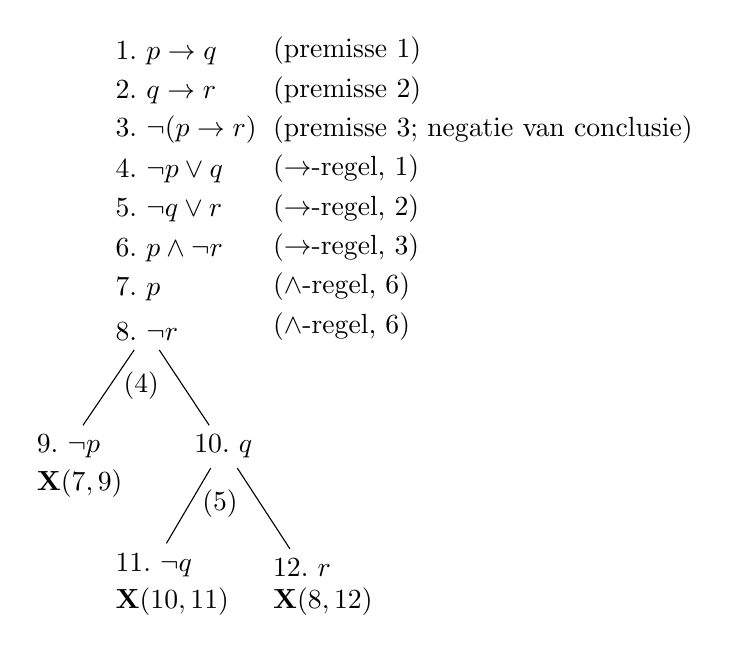
\begin{tikzpicture}[anchor=south west]
\node at (2,6) {$1.\ p\rightarrow q$}; \node at (4,6) {(premisse 1)};
\node at (2,5.5) {$2.\  q\rightarrow r$}; \node at (4,5.5) {(premisse 2)};
\node at (2,5) {$3.\  \neg(p\rightarrow r)$}; \node at (4,5) {(premisse 3; negatie van conclusie)};
\node at (2,4.5) {$4.\  \neg p\lor q$}; \node at (4,4.5) {($\rightarrow$-regel, 1)};
\node at (2,4) {$5.\  \neg q\lor r$}; \node at (4,4) {($\rightarrow$-regel, 2)};
\node at (2,3.5) {$6.\  p\land\neg r$}; \node at (4,3.5) {($\rightarrow$-regel, 3)};
\node at (2,3) {$7.\  p$}; \node at (4,3) {($\land$-regel, 6)};
\node at (2,2.5) (pre) {$8.\  \neg r$}; \node at (4,2.5) {($\land$-regel, 6)};
\node at (1,1) (p1) {$9.\  \neg p$}; \node at (1,0.5) {$\mathbf{X}(7,9)$};
\node at (3,1) (p2) {$10.\  q$};
\draw (p1) -- (pre) -- (p2);
\node at (2.1, 1.75) {$(4)$};
\node at (2,-.5) (p3) {$11.\  \neg q$}; \node at (4,-.5) (p4) {$12.\  r$};
\node at (2,-1) {$\mathbf{X}(10,11)$}; \node at (4,-1) {$\mathbf{X}(8,12)$};
\node at (3.1,0.25) {$(5)$};
\draw (p3) -- (p2) -- (p4);
\end{tikzpicture}
\end{center}
\end{example}

Merk op dat het aantonen dat een formule een contradictie is nu eenvoudig te doen is door het maken van een boom voor de formule zelf (immers, een sluitende boom geeft onvervulbaarheid aan, en contradicties zijn onvervulbaar). Voor het aantonen dat een formule een tautologie is, is een boom voor de negatie van de formule benodigd (immers, de negatie van een tautologie is een contradictie). Om te bewijzen dat iets een formule een contingentie is, zijn helaas wat meer stappen benodigd. Immers dient men dan aan te tonen dat zowel de boom voor de oorspronkelijke formule en de boom voor de negatie van de formule \textit{niet} sluiten\footnote{Als slechts \'e\'en van beide niet sluitende bomen wordt gemaakt, wordt er feitelijk alleen maar aangetoond dat de formule $\varphi$ geen contradictie is (aangetoond door niet sluitende boom voor $\varphi$) \'of dat $\varphi$ geen tautologie is (aangetoond door niet sluitende boom voor $\neg\varphi$).}.


\begin{example} \textit{niet} $\vdash (p\rightarrow q)\rightarrow(q\rightarrow p)$\\
We laten zien hoe met behulp van de boommethode een tegenvoorbeeld kan worden verkregen voor de uitspraak $\vdash (p\rightarrow q)\rightarrow(q\rightarrow p)$ (wat dus zoveel wil zeggen als dat $(p\rightarrow q)\rightarrow(q\rightarrow p)$ g\'e\'en tautologie is). De boom hieronder laat zien dat de verzameling $\neg(p\rightarrow q)\rightarrow(q\rightarrow p))$ vervulbaar is. Geen van de takken van de boom sluit. Een tegenvoorbeeld is bijvoorbeeld te lezen in de linkertak: maak $p$ onwaar en $q$ waar. Hiermee is bewezen dat $\vdash (p\rightarrow q)\rightarrow(q\rightarrow p)$ \textit{niet} geldt!
\begin{center}
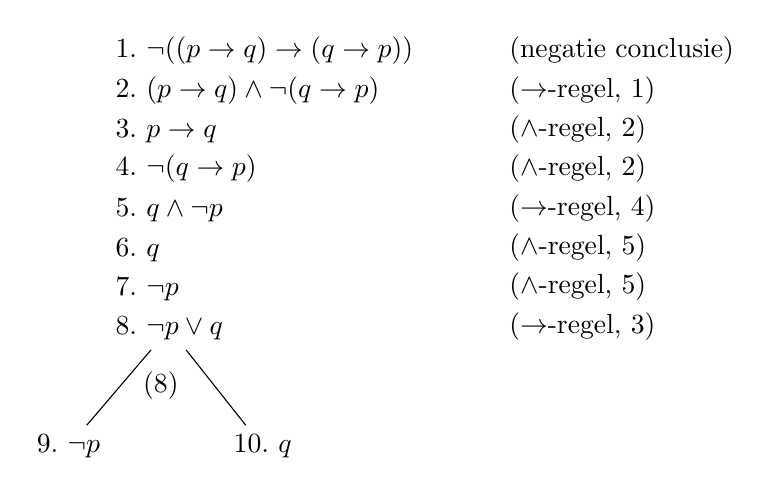
\begin{tikzpicture}[anchor=south west]
\node at (2,6) {$1.\ \neg((p\rightarrow q)\rightarrow(q\rightarrow p))$}; \node at (7,6) {(negatie conclusie)};
\node at (2,5.5) {$2.\ (p\rightarrow q)\land\neg(q\rightarrow p)$}; \node at (7,5.5) {($\rightarrow$-regel, 1)};
\node at (2,5) {$3.\  p\rightarrow q$}; \node at (7,5) {($\land$-regel, 2)};
\node at (2,4.5) {$4.\  \neg(q\rightarrow p)$}; \node at (7,4.5) {($\land$-regel, 2)};
\node at (2,4) {$5.\  q\land\neg p$}; \node at (7,4) {($\rightarrow$-regel, 4)};
\node at (2,3.5) {$6.\  q$}; \node at (7,3.5) {($\land$-regel, 5)};
\node at (2,3) {$7.\  \neg p$}; \node at (7,3) {($\land$-regel, 5)};
\node at (2,2.5) (p1) {$8.\  \neg p\lor q$}; \node at (7,2.5) {($\rightarrow$-regel, 3)};
\node at (1,1) (p2) {$9.\  \neg p$}; \node at (3.5,1) (p3) {$10.\  q$};
\draw (p2) -- (p1) -- (p3);
\node at (2.35, 1.75) {$(8)$};
\end{tikzpicture}
\end{center}
\end{example}

\subsection{Opgaven}
Om de techniek van bewijzen te oefenen, mogen in de volgende opgaven geen waarheidstabellen, gelijkheidswaarheden of tautologi\"en worden gebruikt. Je mag alleen gebruik maken van de in dit hoofdstuk gegeven boommethode.

\begin{exercise}
Bewijs met de boommethode dat:
\begin{enumerate}[label=\textit{\alph*.}]
\item $p\vdash p$
\item $p\wedge q\vdash q$
\item $p\rightarrow q\vdash \neg p\vee q$
\item $\neg p\vdash p\rightarrow q$
\item $\neg(p\vee q)\vdash p\rightarrow q$
\end{enumerate}
\end{exercise}
\begin{exercise} Ga voor elk van de onderstaande beweringen na of dat deze juist danwel onjuist is. Geef in het eerste geval een bewijs met behulp van de boommethode. Construeer in het tweede geval een \textit{tegenvoorbeeld}.
\begin{enumerate}[label=\textit{\alph*.}]
\item $p\rightarrow q$ is een tautologie (d.w.z. $\vdash p\rightarrow q$).
\item $p\rightarrow p$ is een tautologie (d.w.z. $\vdash p\rightarrow p$).
\item $p\leftrightarrow p$ is een tautologie (d.w.z. $\vdash p\leftrightarrow p$).
\item $p\wedge\neg q$ is een contradictie (d.w.z $\not\vdash p\wedge\neg q$ ofwel $\vdash\neg(p\wedge\neg q)$).
\item $p\wedge\neg p$ is een contradictie (d.w.z. $\not\vdash p\wedge\neg p$).
\item $p\leftrightarrow\neg p$ is een contradictie (d.w.z. $\not\vdash p\leftrightarrow\neg p$).
\end{enumerate}
\end{exercise}
\begin{exercise} Bewijs met de boommethode dat:
\begin{enumerate}[label=\textit{\alph*.}]
\item $p, (p\land\neg q)\rightarrow r, \neg (p\land r)\vdash q$.
\item $\neg p\leftrightarrow(q\lor r), p\land r\vdash\neg q$.
\item $p\leftrightarrow(\neg q\lor\neg r), \neg(\neg p\rightarrow r)\vdash \neg q$.
\item $p\rightarrow((q\rightarrow r)\rightarrow s), \neg(p\rightarrow s)\vdash\neg(q\rightarrow r)$.
\item $(p\land q)\rightarrow r,\neg p\lor(p\rightarrow q)\vdash p\rightarrow r$.
\item $(p\rightarrow\neg r)\lor(p\rightarrow q), r\rightarrow p\vdash r\rightarrow q$.
\end{enumerate}
\end{exercise}
\begin{exercise}Ga voor elk van de onderstaande beweringen na of deze juist dan wel onjuist is. Geef in het eerste geval een bewijs met behulp van de boommethode. Construeer in het tweede geval een \textit{tegenvoorbeeld}.
\begin{enumerate}[label=\textit{\alph*.}]
\item $p\rightarrow q,\neg r\rightarrow q\vdash p\rightarrow r$.
\item $\vdash ((p\lor(p\rightarrow q))\rightarrow q)\rightarrow q$.
\item $(p\land q)\rightarrow s, \neg(s\rightarrow t), q\lor t\vdash \neg p$.
\item $\neg p\rightarrow p\vdash p$.
\item $\vdash (p\lor q)\rightarrow (p\land q)$.
\item $\neg p,p\vdash q$.
\end{enumerate}
\end{exercise}
\begin{exercise} Vertaal de volgende redeneringen naar \textit{propositielogica} en ga met behulp van de boommethode na of deze logisch geldig zijn of niet. Produceer in het laatste geval ook een tegenvoorbeeld.
\begin{enumerate}[label=\textit{\alph*.}]
\item \textit{Als Tom nuchter is, dan handelt hij rationeel maar hij is dan wel oninteressant.}\\
\textit{Als hij beleefd en oninteressant is, dan vindt Sylvia hem niet aardig.}\\
\textit{Dus, als Tom nuchter en beleefd is, dan vindt Sylvia hem niet aardig.}
\item\textit{Als Anton lid wordt van de Nederlandse Vereniging van Terraszitters, dan worden Bob en Cees dat ook.}\\
\textit{Als Anton of Bob lid wordt, dan zal David zijn lidmaatschap opzeggen.}\\
\textit{Dus zal David zijn lidmaatschap opzeggen, ongeacht of Cees nou lid wordt of niet.}
\item\textit{Je kunt Hans geloven als je Bert kunt geloven, en omgekeerd.}\\
\textit{Als je noch Hans, noch Bert kunt geloven, dan kun je ook Greetje niet geloven.}\\
\textit{Je kunt Greetje geloven.}\\
\textit{Dus je kunt Bert geloven.}
\end{enumerate}

\end{exercise}

%\section{Natuurlijke deductie *}\label{sec:nat:deduc}
%\begin{remark}
%De stof in deze sectie behoort niet tot de basisstof van het vak en zal niet getentamineerd worden. Ze is enkel toegevoegd voor ge\"interesseerde studenten die \textit{verder} willen dan de gemiddelde student.
%\end{remark}
%
%Eerder, in sectie \ref{sec:boom}, hebben we wat spelregels ge\"introduceerd voor het uitvoeren van deductie. In deze sectie zullen we daarop verder bouwen en alle regels introduceren. We zullen ook elke regel een naam geven, zodat we in motivaties in bewijzen alleen die naam hoeven te noemen in plaats van de hele regel zelf op te schrijven.
%
%Voor afleidingsregels gebruiken we de volgende notatie.
%$$A, B,\ldots \vdash C, D,\ldots$$
%Dit dient gelezen te worden als: als \textit{elk} van de proposities \textit{links} van $\vdash$ waar is of verondersteld wordt waar te zijn, dan mag de waarheid van elke propositie \textit{rechts} van de $\vdash$ geconcludeerd worden.
%
%Een andere veel gebruikte notatie voor hetzelfde doel is de conclusiestreep
%$$\frac{A,B,\ldots}{C,D,\ldots}\text{ betekent hetzelfde als }A,B,\ldots\vdash C,D,\ldots$$
%De afleidingsregels die gelden voor natuurlijke deductie zijn de volgende.
%\begin{center}\begin{tabular}{|lc|}
%\hline\\[-1em]
%& (sub)bewijs beginnend met \\ 
%\textit{deductie} & $A$ (veronderstelling) en eindigend met $B$\\
%& $\qquad \vdash A\rightarrow B$\\[0.5em]
%\hline\\[-1em]
%\textit{modus ponens} & $A, A\rightarrow B\vdash B$\\[0.5em]
%\hline\\[-1em]
%\textit{introductie-$\land$} & $A, B\vdash A\land B$\\[0.5em]
%\hline\\[-1em]
%\textit{eliminatie-$\land$} & $A\land B\vdash A, B$\\[0.5em]
%\hline\\[-1em]
%\textit{introductie-$\lor$} & $A\vdash A\lor B, B\lor A$\\[0.5em]
%\hline\\[-1em]
%\textit{eliminatie-$\lor$} & $A\lor B, A\rightarrow C, B\rightarrow C\vdash C$\\[0.5em]
%\hline\\[-1em]
%\textit{introductie-$\leftrightarrow$} & $A\rightarrow B, B\rightarrow A\vdash A\leftrightarrow B$\\[0.5em]
%\hline\\[-1em]
%\textit{eliminatie-$\leftrightarrow$} & $A\leftrightarrow B\vdash A\rightarrow B, B\rightarrow A$\\[0.5em]
%\hline\\[-1em]
%\textit{introductie-$\neg$} & $B\rightarrow\bot\vdash\neg B$\\[0.5em]
%\hline\\[-1em]
%\textit{introductie-$\bot$} & $A,\neg A\vdash\bot$\\[0.5em]
%\hline\\[-1em]
%\textit{eliminatie-$\bot$} & $\bot\vdash A$\\[0.5em]
%\hline\\[-1em]
%\textit{gevalsonderscheid} & $\vdash A\lor\neg A$\\[0.5em]
%\hline
%\end{tabular}
%\end{center}
%
%Op deze wijze hebben we voor elk van de connectieven een introductieregel waarmee een propositie \textit{bewezen} kan worden waarin dat connectief voorkomt, en voor elk van de binaire connectieven een eliminatie regel waarmee een propositie \textit{gebruikt} kan worden waarin dat connectief voorkomt. Hierin speelt deductie de rol van \textit{introductie-$\rightarrow$} en modus ponens de rol van \textit{eliminatie-$\rightarrow$}. Om historische redenen gebruiken we echter de begrippen deductie en modus ponens.
%
%In plaats van de regel \textit{gevalsonderscheid} hadden we ook een regel $\vdash\top$ kunnen invoeren onder de naam \textit{introductie-$\top$} en een regel $\top\vdash A\lor\neg A$ onder de naam \textit{eliminatie-$\top$}. Deze regels worden echter voornamelijk in combinatie gebruikt, en daarom hebben we de combinatie gelijk maar als regel ingevoerd. Zo kan hij vaak handig worden gebruikt, in het bijzonder om eliminatie-$\lor$ te kunnen toepassen: als we $A\rightarrow C$ en $\neg A\rightarrow C$ hebben afgeleid, kunnen we met deze regel en eliminatie-$\lor$ concluderen dat dan ook $C$ geldt. Hiermee is $C$ in feite bewezen door een gevalsonderscheid tussen $A$ en $\neg A$ te maken. Immers, in de klassieke logica zijn er maar twee gevallen te onderscheiden wat betreft een variabele $A$; deze is waar, of deze is niet waar. Als uit beide gevallen blijkt dat je $C$ kan afleiden, dan geldt dat dus altijd (alle gevallen zijn gedekt).
%
%Er zijn nog wel meer regels te verzinnen. We beperken ons echter tot de hier gegeven lijst.
%
%De systematiek van de lijst kun je opvatten als hulpmiddel om een bewijs te vinden. Zo word je gedwongen om de bijbehorende introductieregel toe te passen als je de geldigheid van een bepaalde propositie wilt bewijzen. Preciezer gezegd:
%\begin{itemize}
%\item Als je de geldigheid van $A\rightarrow B$ wilt bewijzen, moet je deductie toepassen, oftewel je begint met $A$ te stellen en je moet vervolgens $B$ bewijzen.
%\item Als je de geldigheid van $A\land B$ wilt bewijzen, moet je introductie-$\land$ toepassen, oftewel je moet zowel $A$ als $B$ bewijzen.
%\item Als je de geldigheid van $A\lor B$ wilt bewijzen, moet je introductie-$\lor$ toepassen, oftewel je moet $A$ bewijzen of $B$ bewijzen.
%\item Als je de geldigheid van $\neg A$ wilt bewijzen, moet je introductie-$\neg$ toepassen, oftewel je moet $A\rightarrow\bot$ bewijzen, en dat moet je weer met deductie doen. In feite geef je hiermee een \textit{bewijs uit het ongerijmde}.
%\end{itemize}
%
%Als voorbeeld bewijzen we, uitsluitend gebruik makend van deze afleidingsregels dat $(p\rightarrow q)\rightarrow(\neg p\lor q)$ een tautologie is.
%\begin{example}  $(p\rightarrow q)\rightarrow(\neg p\lor q)$ is een tautologie.
%\begin{proof}\mbox{}\\
%\begin{tabular}{lll}
%(1) & $p\rightarrow q$ & (veronderstelling) \\
%(2) & $p\lor\neg p$ & (gevalsonderscheiding) \\
%(3) & \multicolumn{2}{l}{te bewijzen: $p\rightarrow(\neg p\lor q)$}\\
%& \multicolumn{2}{l}{\begin{tabular}{lll}
%  \multicolumn{3}{l}{\textsc{bewijs} van (3):}\\
%  (3.1) & $p$ & (veronderstelling) \\
%  (3.2) & $q$ & (modus ponens: 1, 3.2) \\
%  (3.3) & $\neg p\lor q$ & (intr.-$\lor$: 3.2) \\
%  \multicolumn{2}{l}{\textsc{einde bewijs (3)}} & (deductie)
%\end{tabular}
%}\\
%(4) & \multicolumn{2}{l}{te bewijzen $(\neg p\rightarrow (\neg p\lor q)$}\\
%& \multicolumn{2}{l}{\begin{tabular}{lll}
%  \multicolumn{3}{l}{\textsc{bewijs} van (4):}\\
%  (4.1) & $\neg p$ & (veronderstelling) \\
%  (4.2) & $\neg p\lor q$ & (intr.-$\lor$, 4.1) \\
%  \multicolumn{2}{l}{\textsc{bewijs} van (4)} & (deductie)
%\end{tabular}} \\
%(5) & $\neg p\lor q$ & (elim.-$\lor$: 2, 3, 4) \\
%\multicolumn{2}{l}{\textsc{einde bewijs}} & (deductie)
%\end{tabular}\\
%\end{proof}
%\end{example}
%
%Het is geenszins de bedoeling om een keurslijf van exacte, doch cryptisch opgeschreven bewijzen op te dringen. Integendeel, een in goed Nederlands opgeschreven heldere redenering heeft het grote voordeel dat iedereen het kan volgen. Vaak echter schiet het gewone taalgebruik te kort om een argumentatie in weinig woorden waterdicht te maken. Juist in die gevallen is een strak systeem van groot nut. Wel geldt uiteraard bij alle bewijzen dat ze moeten voldoen aan de hier gegeven spelregels, ook als de verschillende beweringen niet expliciet genummerd zijn. De hier gegeven spelregels zijn niet gegeven om het je moeilijk te maken, maar zijn een weerslag van de consensus over wat correcte en geldige redeneringen zijn, en hopen juist een hulpmiddel te zijn om dergelijke redeneringen gestructureerd te kunnen krijgen.
%
%In de praktijk zal men veelal conclusies trekken, zonder de verantwoording tot in de allerkleinste details op te schrijven. Men geeft dan alleen de grote lijnen weer. Op zich is dat niet zo erg, het hoort bij de ontwikkeling tot beoefenaar van een vak. Naarmate de ontwikkeling vordert worden steeds complexere combinaties tot een geheel. Hierin schuilen uiteraard wel grotere gevaren voor vergissingen! Probeer nooit een bewijs zo ``uit te dunnen'' dat je zelf na een paar dagen moeite hebt om te zien ``hoe het ook weer zat''.
%
%\subsection{Opgaven}
%Om de techniek van deductie te oefenen, mogen in de volgende opgaven geen waarheidstabellen, gelijkheidswaarheden, tautologi\"en of boommethode worden gebruikt. Je mag alleen gebruik maken van de in deze sectie ge\"introduceerde afleidingsregels van deductie.
%
%\begin{exercise}
%Bewijs dat $(p\rightarrow q)\rightarrow((p\land r)\rightarrow(q\land r))$ een tautologie is.
%\end{exercise}
%\begin{exercise}
%Bewijs dat $((p\rightarrow q)\land(q\rightarrow r))\rightarrow(p\rightarrow r)$ een tautologie is.
%\end{exercise}
%\begin{exercise}
%Bewijs dat $((p\rightarrow q)\land(r\rightarrow s)\land p\land r)\rightarrow(q\land s))$ een tautologie is.
%\end{exercise}
%\begin{exercise}
%Bewijs dat $((p\rightarrow q)\land(p\rightarrow\neg q))\rightarrow\neg p$ een tautologie is.
%\end{exercise}
%\begin{exercise}
%Bewijs dat $\neg p\rightarrow(p\rightarrow q)$ een tautologie is.
%\end{exercise}
%\begin{exercise}
%Bewijs dat $(p\rightarrow q)\rightarrow(\neg q\rightarrow\neg p)$ een tautologie is.
%\end{exercise}
%\begin{exercise}
%Bewijs dat $(\neg p\leftrightarrow q)\rightarrow\neg(p\leftrightarrow q)$ een tautologie is.
%\end{exercise}

\chapter{Natuurlijke Deductie en Sequenten}
Een alternatief om logische gevolgtrekking te bewijzen is met behulp van \emph{sequenten-calculus}, en het daaraan gerelateerde systeem van \emph{natuurlijke deductie}. Beide formalismen in dit hoofdstuk volgen uit het werk van Gentzen, die poogde een bewijssysteem te formaliseren dat niet, zoals Hilbert's eerdere systeem, van onvoorwaardelijke tautologi\"en afhankelijk was. Van de twee is sequent-calculus vaak eenvoudiger om een stelling mee te bewijzen, met name omdat de bewijzen meer lineair opgebouwd worden. Natuurlijke deductie vergt wat meer creativiteit, omdat je meer van twee kanten naar elkaar toe moet werken, en heeft de mogelijkheid net iets compactere bewijzen te leveren. Natuurlijke deductiebewijzen hebben daarnaast een interessante link naar programma's en types, in het bijzonder in de functionele stijl. Deze link komt in Sectie~\ref{sec:curry-howard} verder aan bod.

In beide systemen wordt gewerkt met \emph{sequenten}, oftewel voorwaardelijke tautologi\"en. De sequent $\Gamma \vdash \Delta$ of $\Gamma \implies \Delta$\sidenote{De eerste notatie is gebruikelijker voor natuurlijke deductie, de tweede voor sequenten-calculus.} geeft bijvoorbeeld aan dat, zolang de antecedent $\Gamma$ een tautologie is, de consequent $\Delta$ dat ook moet zijn. Een bewijs begint bovenaan met een aantal axioma's, doorgaans van de vorm $A \implies A$; hier worden regels op toegepast om uiteindelijk op de te bewijzen stelling uit te komen. Om een dergelijk bewijs te schrijven begin je doorgaans onderaan en probeer je door het toepassen van de juiste regels op enkel axioma's uit te komen. In dit geval is de stelling onvoorwaardelijk bewezen. Als het niet mogelijk is een bewijs op deze manier te completeren, dan is de stelling op z'n minst afhankelijk bewezen door de overgebleven antecedenten als aannames toe te voegen. 

  \begin{marginfigure}
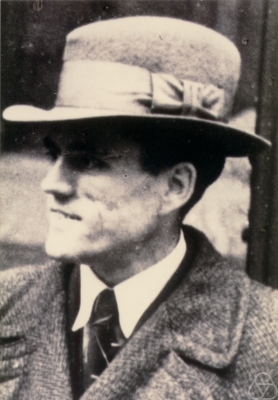
\includegraphics[width=0.6\textwidth]{gentzen.jpg}\\
    Gerhard Gentzen {\scriptsize\emph (Image by Wikipedia)}\\[3mm]
  \end{marginfigure}

\section{Sequenten-calculus}
In het geval van de sequenten-calculus mogen sequenten nul of meerdere antecedenten en consequenten hebben, bijvoorbeeld $A_0, A_1, \dots, A_n \implies B_0, B_1, \dots, B_n$. We interpreteren deze sequent zo dat als elke $A_i$ waar is, tenminste een $B_i$ waar moet zijn.

De regels die we mogen toepassen staan gegeven in Stelling~\ref{th:lk}. De regels zijn onder te verdelen in \emph{structurele regels} (weakening, contraction en exchange), die enkel de structuur van het bewijs veranderen, en \emph{logische regels} die logische connectieven introduceren. De laatste categorie is verder te verdelen in \emph{linker-} en \emph{rechter-regels}, afhankelijk van welke kant van de pijl ze opereren.

\begin{figure}[ht]
\begin{theorem}\label{th:lk} Gentzen Calculus \lk
\paragraph{Axioma's}\mbox{}\\[3mm]
\inference{Ax}{}{A \implies A} (voor atomaire $A$)
\hspace{5mm}
\inference{L\bot}{}{\bot \implies}
\hspace{5mm}
\inference{R\top}{}{\implies \top}

\paragraph{Structurele regels}\mbox{}\\[3mm]
\inference{LW}{\Gamma, \Gamma^\prime \implies \Delta}{\Gamma, A, \Gamma^\prime \implies \Delta}
\hspace{5mm}
\inference{RW}{\Gamma \implies \Delta, \Delta^\prime}{\Gamma \implies \Delta, A, \Delta^\prime}

\vspace{5mm}

\inference{LC}{\Gamma, A, A, \Gamma^\prime \implies \Delta}{\Gamma, A, \Gamma^\prime \implies \Delta}
\hspace{5mm}
\inference{RC}{\Gamma \implies \Delta, A, A, \Delta^\prime}{\Gamma \implies \Delta, A, \Delta^\prime}

\vspace{5mm}

\inference{LE}{\Gamma, A, B, \Gamma^\prime \implies \Delta}{\Gamma, B, A, \Gamma^\prime \implies \Delta}
\hspace{5mm}
\inference{RE}{\Gamma \implies \Delta, A, B, \Delta^\prime}{\Gamma \implies \Delta, B, A, \Delta^\prime}

\vspace{5mm}

\fork{Cut}{\Gamma \implies A, \Delta}{\Sigma, A \implies \Pi}{\Gamma, \Sigma \implies \Delta, \Pi}

\paragraph{Logische regels}\mbox{}\\[3mm]

\fork{L\to}{\Gamma \implies A, \Delta}{B, \Gamma^\prime \implies \Delta^\prime}{\Gamma, A \to B, \Gamma^\prime \implies \Delta, \Delta^\prime}
\hspace{5mm}
\inference{R\to}{\Gamma, A \implies B, \Delta}{\Gamma \implies A \to B, \Delta}

\vspace{5mm}

%\inference{L\land_1}{\Gamma, A \implies \Delta}{\Gamma, A \land B \implies \Delta}
%\hspace{5mm}
%\inference{L\land_2}{\Gamma, B \implies \Delta}{\Gamma, A \land B \implies \Delta}
\inference{L\land}{\Gamma, A, B, \Gamma^\prime \implies \Delta}{\Gamma, A \land B, \Gamma^\prime \implies \Delta}
\hspace{5mm}
\fork{R\land}{\Gamma \implies \Delta, A, \Delta^\prime}{\Gamma \implies \Delta, B, \Delta^\prime}{\Gamma \implies \Delta, A \land B, \Delta^\prime}

\vspace{5mm}

\fork{L\lor}{\Gamma, A, \Gamma^\prime \implies \Delta}{\Gamma, B, \Gamma^\prime \implies \Delta}{\Gamma, A \lor B, \Gamma^\prime \implies \Delta}
\hspace{5mm}
%\inference{R\lor_1}{\Gamma \implies \Lambda, A, \Delta}{\Gamma \implies \Lambda, A \lor B, \Delta}
%\hspace{5mm}
%\inference{R\lor_2}{\Gamma \implies \Lambda, B, \Delta}{\Gamma \implies \Lambda, A \lor B, \Delta}
\inference{R\lor}{\Gamma \implies \Delta, A, B, \Delta^\prime}{\Gamma \implies \Delta, A \lor B, \Delta^\prime}

\vspace{5mm}

\inference{L\neg}{\Gamma \implies A, \Delta}{\Gamma, \neg A \implies \Delta}
\hspace{5mm}
\inference{R\neg}{\Gamma, A \implies \Delta}{\Gamma \implies \neg A, \Delta}
\end{theorem}
\end{figure}

%\paragraph{Rules for Quantifiers}\mbox{}\\[3mm]
%\inference{L\forall}{\Gamma, A[t/x], \Sigma \implies \Delta}{\Gamma, \forall x A, \Sigma \implies \Delta}
%\hspace{5mm}
%\inference{R\forall}{\Gamma \implies \Lambda, A[z/x], \Theta}{\Gamma \implies \Lambda, \forall x A, \Theta}
%
%\vspace{5mm}
%
%\inference{L\exists}{\Gamma, A[z/x], \Sigma \implies \Delta}{\Gamma, \exists x A, \Sigma \implies \Delta}
%\hspace{5mm}
%\inference{R\exists}{\Gamma \implies \Lambda, A[t/x], \Theta}{\Gamma \implies \Lambda, \exists x A, \Theta}


\subsection{Voorbeelden}
We beginnen met een eenvoudig voorbeeld, en zullen daarna een iets groter gevolg bewijzen.

\begin{example}\label{ex:lk:helloworld}
Geef een afleiding in \lk{} voor de sequent $P \land Q \implies P$.

We beginnen met hetgeen we willen bewijzen als eindsequent:

\begin{prooftree}
\lksorry{$P \land Q \implies P$}
\end{prooftree}

Nu moeten we op zoek naar een afleidingsregel met de juiste sequent onder de streep. Dit kan eigenlijk altijd een structurele regel zijn, maar deze werken eigenlijk alleen om een sequent in een andere vorm te schrijven, dus we proberen eerst de logische regels. Als we een logische regel vinden die \emph{net niet} past, dan kunnen we op zoek naar een structurele regel als \enquote{adapter}. In dit geval is er maar \'e\'en logisch connectief, een $\land$ links, dus zouden we de $L\land$ regel kunnen proberen:

\begin{prooftree}
  \lksorry[$L\land$]{$P \land Q \implies P$}
\end{prooftree}

Nu kunnen we boven de streep invullen. De Griekse letters staan voor een set logische zinnen; in het geval van $\Gamma$ is deze leeg omdat er niets anders links van de pijl staat. $A$ en $B$ in de regel komen overeen met $P$ en $Q$ in onze formule. $\Delta$ staat in deze regel voor alles achter de pijl, in ons geval $P$. Aan $\Gamma$ en $\Delta$ verandert er niets, maar links van de komma splitsen we $P \land Q$ op in de losse zinnen $P$ en $Q$. Als we dit in het template invullen krijgen we de volgende situatie:

\begin{prooftree}
\lksorry{$P, Q \implies P$}
\lklconj{$P \land Q \implies P$}
\end{prooftree}

Nu is het tijd om een structurele regel toe te passen. We zij bijna willen toe naar het axioma $P \implies P$, maar we moeten nog van de $Q$ af zien te komen. Dit kan met weakening links, waarbij de $A$ onder de streep de in ons geval $Q$ is. Na toepassen van de regel zijn we deze boven de streep vergeten:

\begin{prooftree}
\lksorry{$P \implies P$}
\lklcontr{$P, Q \implies P$}
\lklconj{$P \land Q \implies P$}
\end{prooftree}

Nu we een Axioma hebben hoeven we deze alleen nog te markeren en is ons bewijs klaar:

\begin{prooftree}
\lkax{$P \implies P$}
\lklcontr{$P, Q \implies P$}
\lklconj{$P \land Q \implies P$}
\end{prooftree}
\hfill\qed

\end{example}

\begin{example}\label{ex:lk:trans}
Laten we nu kijken naar een iets groter voorbeeld: $P \to Q, Q \to R \implies P \to R$, oftewel als $P$ voldoende is om $Q$ aan te tonen, en $Q$ voldoende is om $R$ aan te tonen, dan kunnen we $P$ als direct bewijs voor $R$ gebruiken. Voor dit bewijs zullen we ons voor de tussenstappen tot de logische regels beperken. De structurele regels worden wel meegenomen, maar niet als losse stappen in de uitleg.

\begin{prooftree}
\lksorry{$P \to Q, Q \to R \implies P \to R$}
\end{prooftree}

  We beginnen wederom met de te bewijzen sequent onder de streep. In dit bewijs hebben we drie connectieven om mee aan de slag te gaan, specifiek drie implicaties. Als we kijken naar de regels uit Stelling~\ref{th:lk}, dan zien we dat $R\!\to$ eenvoudiger oogt dan $L\!\to$, dus dat zou een logisch begin zijn. In plaats van te splitsen hoeven we enkel het antecedent van de implicatie naar links te halen:

\begin{prooftree}
\lksorry{$P \to Q, Q \to R, P \implies R$}
\lkrimpl{$P \to Q, Q \to R \implies P \to R$}
\end{prooftree}

Nu hebben we nog twee operatoren over, de implicaties aan de rechterkant. Voor de $L\!\to$ regel moeten we een beetje schuiven om de juiste termen aan de juiste kant te krijgen, maar met een enkele exchange kunnen we $Q \to R$ splitsen. We krijgen dan links $Q$ als consequent en rechts $R$ als antecedent. Dit geeft de sequenten $P \to Q, P \implies Q$ en $R \implies R$. Dat zou moeten lukken.

\begin{prooftree}
  \lksorry{$P \to Q, P \implies Q$}

  \lkax{$R \implies R$}

\lklimpl{$P \to Q, P, Q \to R \implies R$}
\lklexch{$P \to Q, Q \to R, P \implies R$}
\lkrimpl{$P \to Q, Q \to R \implies P \to R$}
\end{prooftree}

Rechts zijn we meteen klaar, dus rest ons de linkerkant. Deze sequent is een enkele exchange verwijderd van een modus ponens, $P, P \to Q \implies Q$. Om deze weg te werken gebruiken we nogmaals de $L\to$ regel, die ons bij de laatste twee axioma's brengt:

\begin{prooftree}
    \lkax{$P \implies P$}

    \lkax{$Q \implies Q$}

  \lklimpl{$P, P \to Q \implies Q$}
  \lklexch{$P \to Q, P \implies Q$}

  \lkax{$R \implies R$}

\lklimpl{$P \to Q, P, Q \to R \implies R$}
\lklexch{$P \to Q, Q \to R, P \implies R$}
\lkrimpl{$P \to Q, Q \to R \implies P \to R$}
\end{prooftree}
\hfill\qed
\end{example}

%We zien hier dat de structurele stappen in een sequentenbewijs een fors deel van de totale  afleiding kunnen zijn. Om bewijzen iets te versimpelen bestaan er alternatieve formulaties van de sequenten-calculus, waar logische zinnen niet in een lijst, maar in een multiset worden beschouwd. In degrelijke formulaties is de volgorde niet langer van belang. Voor klassieke logica kunnen we zelfs nog verder gaan en ook weakening en contraction stilzwijgend negeren, maar verderop zullen we zien dat deze regels wel degelijk betekenis hebben als we in Hoofdstuk~\ref{ch:systemen} logische systemen gaan tegenkomen die deze stappen niet zonder meer toelaten.

\subsection{De cut-regel}
De cut-regel is een zekere zin discutabel. Elke stelling die met cut bewezen kan worden, kan ook zonder cut worden bewezen. De set van geldige stellingen verandert dus niet door deze regel toe te voegen, en in principe heeft een systeem met zo min mogelijk regels de voorkeur. Desalniettemin kan de cut-regel helpen om proofs overzichtelijk te houden. Beschouw de twee bewijzen van het sequent $A \land B, \neg A \lor C \implies C$ hieronder.

\begin{prooftree}
  \lkax{$A\implies A$}
  \lklweak{$A, B \implies A$}
  \lklconj{$A \land B \implies A$}

    \lkax{$A\implies A$}
    \lklneg{$A, \neg A\implies$}
    \lklweak{$A, \neg A \implies C$}

    \lkax{$C \implies C$}
    \lklweak{$A, C \implies C$}
  \lkldisj{$\neg A \lor C, A \implies C$}

\lkcut{$A \land B, \neg A \lor C \implies C$}
\end{prooftree}

Met cut splitsen we het sequent in twee makkelijker te bewijzen stellingen. Doen we dat niet, dan hebben we uiteindelijk wat meer structurele regels nodig:

\begin{prooftree}
  \lkax{$A \implies A$}
  \lklneg{$A, \neg A \implies$}
  \lklweak{$A, B, \neg A \implies$}
  \lkrweak{$A, B, \neg A \implies C$}

  \lkax{$C \implies C$}
  \lklweak{$B, C \implies C$}
  \lklweak{$A, B, C \implies C$}
\lkldisj{$A, B, \neg A \lor C \implies C$}
\lklconj{$A \land B, \neg A \lor C \implies C$}
\end{prooftree}

\subsection{Opgaven}
\begin{exercise}\mbox{}\\
  Geef een afleiding in \lk{} voor de sequenten behorend bij equivalenties 9, 10, 11 en 12 uit Stelling~\ref{th:equiv}. Omdat we met sequenten-calculus gevolgtrekkingen bewijzen, interpreteren we de elke equivalentie als een tweetal gevolgtrekkingen: heen en terug.

\begin{enumerate}[label=\textit{\alph*.}]
\item $\neg(p\lor q) \implies \neg p\land\neg q$ \\
\item $\neg p\land\neg q \implies \neg(p\lor q)$ \\
\item $\neg(p\land q) \implies \neg p \lor\neg q$ \\
\item $\neg p \lor\neg q \implies \neg(p\land q)$ \\
\item $(p\lor q)\land r \implies (p\land r)\lor(q\land r)$ \\
\item $(p\land r)\lor(q\land r) \implies (p\lor q)\land r$  \\
\item $(p\land q)\lor r \implies (p\lor r)\land(q\lor r)$ \\
\item $(p\lor r)\land(q\lor r) \implies (p\land q)\lor r$  \\
\end{enumerate}
\end{exercise}

\section{Natuurlijke Deductie}
Een vergelijkbaar systeem is de Natuurlijke Deductie. De notatie die we hiervoor gebruiken lijkt erg op die van de Sequenten-calculus, met als voornaamste verschillen dat we nu de $\vdash$ gebruiken in plaats van $\implies$, en dat we achter de $\vdash$\sidenote{In de literatuur zul je ook een variant tegenkomen waar de hypothesen helemaal niet in de sequent worden bijgehouden en de $\vdash$ dus ontbreekt. Dit vergt iets meer aandacht wat er met hypothesen en implicaties gebeurt, dus wij zullen de hypothesen als antecedenten in het sequent bijhouden.} maar \'e\'en logische zin mogen hebben. Dat betekent ook dat we niet dezelfde regels kunnen gebruiken: $R\lor$ zou bijvoorbeeld een disjunctie moeten splitsen, maar we kunnen niet beide termen tegelijk kwijt. Hierdoor ontstaat een nieuwe set regels, weergegeven in Stelling~\ref{th:nd}. Ook hierverdelen we der regels in een aantal soorten, specifiek onderscheiden we voor logische regels nu de \emph{introductie}- en \emph{eliminatie}-regels. De introductie-regels lijken meestal redelijk op de rechter-regels van \lk{}, maar  de eliminatie-regels werken vaak net iets anders. Een gevolg hiervan is dat we wat meer inzicht moeten gebruiken: we werken niet langer van de conclusie naar de aannames, maar van beide naar elkaar toe.

\begin{figure}[ht]
\begin{theorem}\label{th:nd} Natuurlijke Deductie
\paragraph{Axioma's}\mbox{}\\[3mm]
\inference{Id}{}{A \vdash A}

\paragraph{Structurele regels}\mbox{}\\[3mm]
\inference{W}{\Gamma \vdash B}{\Gamma, A \vdash B}
\hspace{5mm}
\inference{C}{\Gamma, A, A \vdash B}{\Gamma, A \vdash B}
\hspace{5mm}
\inference{E}{\Gamma, \Delta \vdash A}{\Delta, \Gamma \vdash A}

\vspace{4mm}

\fork{Cut}{\Gamma \vdash A}{\Sigma, A, \Pi \vdash \Delta}{\Sigma, \Gamma, \Pi \vdash \Delta}
\paragraph{Logische regels}\mbox{}\\[3mm]
\inference{\to I}{\Gamma, A \vdash B}{\Gamma \vdash A \to B}
\hspace{5mm}
\fork{\to E}{\Gamma \vdash A \to B}{\Delta \vdash A}{\Gamma, \Delta \vdash B}

\vspace{4mm}

\fork{\land I}{\Gamma \vdash A}{\Delta \vdash B}{\Gamma, \Delta \vdash A \land B}
\hspace{5mm}
\fork{\land E}{\Gamma \vdash A \land B}{\Delta, A, B \vdash C}{\Gamma, \Delta \vdash C}

\vspace{4mm}
\inference{\lor I_1}{\Gamma \vdash A}{\Gamma \vdash A\lor B}
\hspace{5mm}
\inference{\lor I_2}{\Gamma \vdash B}{\Gamma \vdash A\lor B}

\vspace{4mm}

\trifork{\lor E}{\Gamma \vdash A \lor  B}{\Delta, A \vdash C}{\Delta, B \vdash C}{\Gamma, \Delta \vdash C}

\vspace{4mm}
\inference{\neg I}{\Gamma, A \vdash \bot}{\Gamma \vdash \neg A}
\hspace{5mm}
\inference{\neg E}{\Gamma, \neg A \vdash \bot}{\Gamma \vdash A}

\vspace{4mm}
\fork{\bot I}{\Gamma \vdash \neg A}{\Delta \vdash A}{\Gamma, \Delta \vdash \bot}
\hspace{5mm}
\inference{\bot E}{\Gamma \vdash \bot}{\Gamma \vdash A}

\end{theorem}
\end{figure}

\subsection{Voorbeelden}
Ook voor natuurlijke deductie lopen we twee voorbeelden door.

\begin{example}\label{ex:nd:export}
  Geef een afleiding in natuurlijke deductie voor de sequent $(P \land Q) \to R \vdash P \to (Q \to R)$. We beginnen weer met de conclusie en gaan van hieruit naar boven werken.

\begin{prooftree}
\ndsorry{$(P \land Q) \to R \vdash P \to (Q \to R)$}
\end{prooftree}

Net als bij het voorbeeld in \lk{} kunnen we het antecedent van een implicatie naar links halen; hoewel we rechts exact een term willen hebben staan, is die beperking er links niet. We voeren deze stap tweemaal uit, waarna we alleen nog $R$ hoeven te bewijzen:

\begin{prooftree}
\ndsorry{$(P \land Q) \to R, P, Q \vdash R$}
\ndimpli{$(P \land Q) \to R, P \vdash Q \to R$}
\ndimpli{$(P \land Q) \to R \vdash P \to (Q \to R)$}
\end{prooftree}

  Nu wordt het iets meer puzzelen. De enige connectief waar we iets mee kunnen is de implicatie links van de pijl --- de conjunctie staat binnen de haakjes, dus daar kunnen we nu nog niet bij. Er zijn twee regels die over implicaties gaan, en de introductie-regel hebben we zo vaak als kon toegepast. We zullen dus implicatie-eliminatie moeten toepassen. Deze heeft onder de streep de sequent $\Gamma, \Delta \vdash B$ staan, waarbij $B$ een logische zin is, en $\Gamma$ en $\Delta$ een serie zinnen is. Voor $B$ matchen we $R$, dus boven de streep krijgen we links $\Gamma \vdash A \to R$ en rechts $\Delta \vdash A$. Nu moeten we voor $\Gamma$, $\Delta$ en $A$ een invulling kiezen. De termen voor de turnstile onder de streep gaan we over $\Gamma$ en $\Delta$ verdelen\sidenote{Strict genomen moeten we voor $\Gamma$ de eerste termen tot een bepaald punt nemen, en de rest in $\Delta$ stoppen. Voor nu negeren we dat even om te bepalen hoe we willen verdelen, dan kunnen we daarna de structurele regels toevoegen om dat kloppend te maken.}, en wel op zo'n manier dat we aan $\Gamma$ genoeg hebben om $A \to R$ te bewijzen en de rest voor het bewijs van $A$ kunnen gebruiken. Als we voor $A$ de term $P \land Q$ kiezen, dan moeten we links $(P \land Q) \to R \vdash (P \land Q) \to R$ bewijzen: een axioma. We houden dan rechts $P, Q \vdash P \land Q$ over, wat ook te doen moet zijn:

\begin{prooftree}
  \ndax{$(P \land Q) \to R \vdash (P \land Q) \to R$}
  \ndsorry{$P, Q \vdash P \land Q$}
\ndimple{$(P \land Q) \to R, P, Q \vdash R$}
\ndimpli{$(P \land Q) \to R, P \vdash Q \to R$}
\ndimpli{$(P \land Q) \to R \vdash P \to (Q \to R)$}
\end{prooftree}

De laatste stap is weer vrij eenvoudig: met conjunctie introductie splitsen we wederom de antecedenten, en moeten we met de eerste termen $P$ bewijzen en de laatste termen $Q$. Door $\Gamma$ als $P$ te kiezen en $\Delta$ als $Q$ hebben we twee axioma's, en hebben we geen structurele regel hoeven toepassen!

\begin{prooftree}
  \ndax{$(P \land Q) \to R \vdash (P \land Q) \to R$}
    \ndax{$P \vdash P$}
    \ndax{$Q \vdash Q$}
  \ndconji{$P, Q \vdash P \land Q$}
\ndimple{$(P \land Q) \to R, P, Q \vdash R$}
\ndimpli{$(P \land Q) \to R, P \vdash Q \to R$}
\ndimpli{$(P \land Q) \to R \vdash P \to (Q \to R)$}
\end{prooftree}
\hfill\qed
\end{example}


\begin{example}\label{ex:nd:demorgan}
  Geef een afleiding in natuurlijke deductie voor de sequent $\vdash \neg (P \land Q) \to \neg P \lor \neg Q$. We beginnen weer met de conclusie en gaan van hieruit naar boven werken.

\begin{prooftree}
\ndsorry{$\vdash \neg (P \land Q) \to \neg P \lor \neg Q$}
\end{prooftree}

De eerste stap is wederom de implicatie introduceren om zoveel mogelijk naar links te halen:
\begin{prooftree}
\ndsorry{$\neg (P \land Q) \vdash \neg P \lor \neg Q$}
\ndimpli{$\vdash \neg (P \land Q) \to \neg P \lor \neg Q$}
\end{prooftree}

Nu lijkt het misschien voordehandliggend om de disjunctie te introduceren, maar dit is helaas een doodlopend pad: we moeten dan een van beide kiezen, maar hebben nog geen heldere route naar een bewijs vanaf dat punt. In plaats daarvan gaan we een tweetal stappen toepassen om een bewijs uit het ongerijmde uit te voeren: we nemen het tegengestelde van onze conclusie aan, en tonen aan dat dit tot een contradictie leidt. Dus in plaats van $\neg (P \land Q) \vdash \neg P \lor \neg Q$ willen we nu $\neg (P \land Q), \neg (\neg P \lor \neg Q) \vdash \bot$ bewijzen. We tonen daarmee aan dat het tegenovergestelde dat we hebben aangenomen, $\neg (\neg P \lor \neg Q)$, niet waar kan zijn, dus dat de originele stelling $\neg P \lor \neg Q$ wel moet kloppen.

Om aan een contradictie te komen gaan we vervolgens splitsen. We nemen een deel van de aannames en bewijzen hier een willekeurige $A$ mee, en met de rest bewijzen we het tegendeel. Als de stelling zowel $A$ als $\neg A$ waar maakt, dan is het een contradictie.

\begin{prooftree}
  \ndsorry{$\neg (P \land Q) \vdash \neg A$}
  \ndsorry{$\neg (\neg P \lor \neg Q) \vdash A$}

\ndboti{$\neg (P \land Q), \neg (\neg P \lor \neg Q) \vdash \bot$}
\ndnege{$\neg (P \land Q) \vdash \neg P \lor \neg Q$}
\ndimpli{$\vdash \neg (P \land Q) \to \neg P \lor \neg Q$}
\end{prooftree}

Laten we voor $A$ de zin $P \land Q$ kiezen. De linkertak is dan automatisch klaar, en de rechtertak krijgt een conjunctie waar we op kunnen splitsen. Voor de conjunctie-introductie moeten we onze aannames verdelen over beide takken, en we hebben maar een aanname, dus voordat we dat doen maken we snel even een kopie zodat beide takken hetzelfde uitgangspunt hebben:

\begin{prooftree}
  \ndax{$\neg (P \land Q) \vdash \neg (P \land Q)$}

    \ndsorry{$\neg (\neg P \lor \neg Q) \vdash P$}
    \ndsorry{$\neg (\neg P \lor \neg Q) \vdash Q$}
  \ndconji{$\neg (\neg P \lor \neg Q), \neg (\neg P \lor \neg Q) \vdash P \land Q$}
  \ndcontr{$\neg (\neg P \lor \neg Q) \vdash P \land Q$}

\ndboti{$\neg (P \land Q), \neg (\neg P \lor \neg Q) \vdash \bot$}
\ndnege{$\neg (P \land Q) \vdash \neg P \lor \neg Q$}
\ndimpli{$\vdash \neg (P \land Q) \to \neg P \lor \neg Q$}
\end{prooftree}

De twee takken zijn nu nagenoeg hetzelfde. Laten we eerst de linkertak oplossen, en daarna de oplossing kopi\"eren en aanpassen voor de rechtertak.  Links lijken we niet direct heel veel te kunnen, anders dan nog een bewijs uit het ongerijmde trekken. Van $P$ maken we $\neg P$, en tonen aan dat $\neg (\neg P \lor \neg Q)$ en $\neg P$ een contradictie vormen. We mogen wederom zelf de $A$ kiezen die tegelijk waar als niet waar moet zijn met deze twee aannames.  We hebben een dubbele negatie in $\neg (\neg P \lor \neg Q)$, dus als we kunnen aantonen dat $\neg P \vdash \neg P \lor \neg Q$ dan zijn we klaar. Dat laatste is niet heel lastig, als we weten dat $\neg P$ dan kunnen we daar een disjunctie mee maken om de tweede term, $\neg Q$ erbij te verzinnen --- omdat we $\neg P$ al weten maakt de andere kant niet meer uit.

\begin{wprooftree}
  \ndax{$\neg (P \land Q) \vdash \neg (P \land Q)$}

      \ndax{$\neg (\neg P \lor \neg Q) \vdash \neg (\neg P \lor \neg Q)$}

      \ndax{$\neg P \vdash \neg P$}
      \nddisjia{$\neg P \vdash \neg P \lor \neg Q$}

    \ndboti{$\neg (\neg P \lor \neg Q), \neg P \vdash \bot$}
    \ndnege{$\neg (\neg P \lor \neg Q) \vdash P$}

    \ndsorry{$\neg P \vdash \neg P \lor \neg Q$}

  \ndconji{$\neg (\neg P \lor \neg Q), \neg (\neg P \lor \neg Q) \vdash P \land Q$}
  \ndcontr{$\neg (\neg P \lor \neg Q) \vdash P \land Q$}

\ndboti{$\neg (P \land Q), \neg (\neg P \lor \neg Q) \vdash \bot$}
\ndnege{$\neg (P \land Q) \vdash \neg P \lor \neg Q$}
\ndimpli{$\vdash \neg (P \land Q) \to \neg P \lor \neg Q$}
\end{wprooftree}

Om het bewijs af te ronden kunnen we de stappen van de linkertak overnemen en toepassen op de rechtertak, met als enige verschil dat we nu de andere variant van de disjunctie-introductie moeten nemen.

\begin{wprooftree}
  \ndax{$\neg (P \land Q) \vdash \neg (P \land Q)$}

      \ndax{$\neg (\neg P \lor \neg Q) \vdash \neg (\neg P \lor \neg Q)$}

      \ndax{$\neg P \vdash \neg P$}
      \nddisjia{$\neg P \vdash \neg P \lor \neg Q$}

    \ndboti{$\neg (\neg P \lor \neg Q), \neg P \vdash \bot$}
    \ndnege{$\neg (\neg P \lor \neg Q) \vdash P$}

      \ndax{$\neg (\neg P \lor \neg Q) \vdash \neg (\neg P \lor \neg Q)$}

      \ndax{$\neg Q \vdash \neg Q$}
      \nddisjib{$\neg Q \vdash  \neg P \lor \neg Q$}

    \ndboti{$\neg (\neg P \lor \neg Q), \neg Q \vdash \bot$}
    \ndnege{$\neg (\neg P \lor \neg Q) \vdash Q$}
  \ndconji{$\neg (\neg P \lor \neg Q), \neg (\neg P \lor \neg Q) \vdash P \land Q$}
  \ndcontr{$\neg (\neg P \lor \neg Q) \vdash P \land Q$}

\ndboti{$\neg (P \land Q), \neg (\neg P \lor \neg Q) \vdash \bot$}
\ndnege{$\neg (P \land Q) \vdash \neg P \lor \neg Q$}
\ndimpli{$\vdash \neg (P \land Q) \to \neg P \lor \neg Q$}
\end{wprooftree}
\hfill\qed
\end{example}

\begin{aside}[Fitch' Systeem]
  Voor natuurlijke deductie bestaan verschillende notaties. Een belangrijk alternatief is de notatie van Fitch, waarbij stappen onder elkaar worden gezet en nieuwe aannames met indentatie worden aangegeven. Ondanks dat dit er heel anders uitziet, leidt dit systeem tot dezelfde bewijzen, zoals bijvoorbeeld het bewijs hieronder. Vergelijk dit met het bewijs in Voorbeeld~\ref{ex:nd:export}: dezelfde stappen worden in dezelfde volgorde genomen. Het systeem van Fitch heeft als voordeel dat het makkelijk in een lopende tekst te verwerken is, maar is iets minder flexibel voor alternatieve logica's omdat het structurele regels buiten beschouwing laat. Daarnaast zien we deze vorm minder vaak in de context van het Curry-Howard Isomorfisme.

$$\begin{nd}
  \hypo {1} {(P \land Q) \to R}
  \open
  \hypo {2} {P}
  \open
  \hypo {3} {Q}
  \have {4} {P \land Q}      \ai{2,3}
  \have {5} {R}              \by{$\to$E}{1,4}
  \close
  \have {6} {Q \to R}        \by{$\to$I}{3-5}
  \close
  \have {7}{P \to (Q \to R)} \by{$\to$I}{2-6}
\end{nd}$$
\hfill\qed
\end{aside}

\subsection{Opgaven}\label{ex:ndc}
\begin{exercise}\mbox{}\\
Geef een afleiding in natuurlijke deductie voor de resterende gevolgtrekkingen behorend bij equivalenties 9, 10, 11 en 12 uit Stelling~\ref{th:equiv}.

\begin{enumerate}[label=\textit{\alph*.}]
\item $\neg(p\lor q) \vdash \neg p\land\neg q$ \\
\item $\neg p\land\neg q \vdash \neg(p\lor q)$ \\
\item $\neg p \lor\neg q \vdash \neg(p\land q)$ \\
\item $(p\lor q)\land r \vdash (p\land r)\lor(q\land r)$ \\
\item $(p\land r)\lor(q\land r) \vdash (p\lor q)\land r$  \\
\item $(p\land q)\lor r \vdash (p\lor r)\land(q\lor r)$ \\
\item $(p\lor r)\land(q\lor r) \vdash (p\land q)\lor r$  \\
\end{enumerate}
\end{exercise}

\newpage
\section{Het Curry-Howard Isomorfisme}\label{sec:curry-howard}

  \begin{marginfigure}

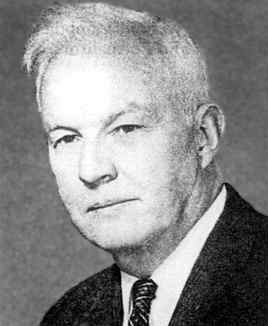
\includegraphics[width=0.6\textwidth]{Curry.jpeg}\\
    Haskell Curry {\scriptsize\emph (Image by University of St. Andrews)}\\[3mm]
  \end{marginfigure}
  \begin{marginfigure}
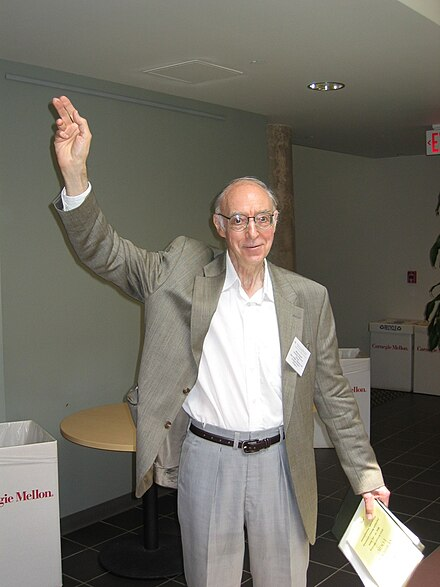
\includegraphics[width=0.6\textwidth]{William_Alvin_Howard_May_2004.jpg}\\
    William Alvin Howard {\scriptsize\emph (Image by Wikipedia)}\\[3mm]
  \end{marginfigure}

Hoewel sequenten-calculus en natuurlijke deductie uiteindelijk dezelfde logische stellingen kunnen bewijzen, en een bewijs met sequenten-calculus vaak eenvoudiger te vinden is door het methodisch toepassen van regels, is er een goede reden om natuurlijke deductie in te zetten: bewijzen met natuurlijke deductie tonen een \'e\'en-op\'e\'en overeenkomst (een \emph{isomorfisme} met computerprogramma's. Dat wil zeggen dat een bewijs direct vertaald kan worden naar een programma, dat daarmee door de computer geverifieerd kan worden, en dat we (in de juiste context) programma's niet hoeven te testen, maar de correctheid wiskundig kunnen bewijzen. Het isomorfisme toont zich daarnaast op een tweede niveau, in een directe overeenkomst tussen typen en logische formules. De overeenkomst is ontdekt door de Amerikaanse wiskundige en computer-wetenschapper Haskell Curry en de logicus William Alvin Howard, in eerste instantie in termen van Intuitionistische Logica (zie Sectie~\ref{sec:il}) en Curry's \emph{Lambda Calculus}\sidenote{De Lambda calculus vormt de basis voor het functionele programmeerparadigma, dat verschilt van imperatieve code zoals we die uit Python gewend zijn doordat alles als onveranderbaar wordt beschouwd. Dit geeft een meer wiskundige manier van programmeren, waar de focus ligt op het combineren van functies en recursie de plaats van loops inneemt. Dankzij het Curry-Howard isomorfisme is getypeerde functionele code vaak aanzienlijk minder gevoelig voor bugs.}, maar uit verder onderzoek is voor vrijwel iedere consistente logica een programmeer-tegenhanger bestond (en vice versa). In de tabel hieronder staat een selectie van termen die met behulp van het isomorfisme vertaald kunnen worden; dit biedt de mogelijkheid om kennis uit verschillende onderzoeksgebieden met elkaar te combineren.\\[5mm]

\begin{tabular}{l l}
  \bf Logica & \bf Programmeren \\
  Implicatie & Functietype \\
  Conjunctie & Producttypes (tuples) \\
  Disjunctie & Somtypes (disjunctive union) \\
  $\top$ & Unit-type \\
  $\bot$ & Leeg type \\
  Universele kwantor & $\Pi$-type \\
  Existenti\"ele kwantor & $\Sigma$-type \\
  Hypothesen & Vrije variabelen \\
  Implicatie-eliminatie & Functie-applicatie \\
  Implicatie-introductie & Abstractie \\
  Wet van Peirce (klassieke logica) & voortzettings-manipulatie \\
\end{tabular}\\[5mm]


\begin{aside}[Curry-Howard-Lambek en HoTT]
  \begin{marginfigure}
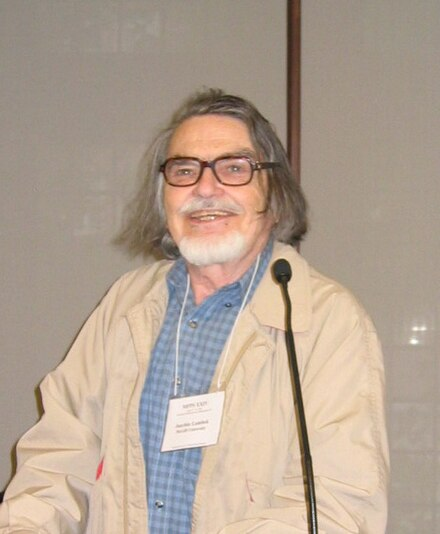
\includegraphics[width=0.6\textwidth]{Lambek_Joachim.jpg}\\
    Joachim Lambek {\scriptsize\emph (Image by Wikipedia)}\\[3mm]
  \end{marginfigure}

  In de jaren '70 koppelde Joachim Lambek het Curry-Howard isomorfisme via \emph{Cartesiaanse gesloten categorie\"en} aan de Categorie-theorie, een abstract maar erg krachtig wiskundige onderzoeksveld, waarbij gekeken wordt naar functies tussen objecten (zoals we dat ook met verzamelingen hebben gezien), maar dan zonder de interne elementen van een verzameling te beschouwen. Met wat slimme wiskundige trucs kunnen we toch heel veel over objecten zeggen zonder \enquote{erin} te mogen kijken, wat tot theori\"en leidt die heel breed toepasbaar zijn. Ze kunnen immers niet op inwendige details berusten, zolang ze hier niets van af weten. Inzichten die hiermee zijn opgedaan zijn van fundamenteel belang in experimentele programmeertalen. Met het werk van Lambek is het mogelijk alle begrippen uit logica en programmeer- en type-theorie in verband te brengen met nog breder wiskundig onderzoek.

  \begin{marginfigure}
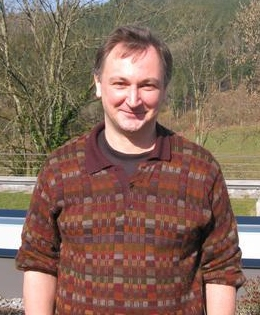
\includegraphics[width=0.6\textwidth]{VladimirVoevodsky.jpg}\\
    Vladimir Voevodsky {\scriptsize\emph (Image by Wikipedia)}\\[3mm]
  \end{marginfigure}

Inmiddels is door Vladimir Voevodsky op deze drie-eenheid doorgebouwd in de \emph{Homotopie Type-theorie}, waarmee hij een nieuw fundament onder de wiskunde probeerde te leggen op basis van computatie en formele software. Homotopie als wiskundig begrip gaat over een zekere zin van gelijkvormigheid van objecten, waarbij bepaalde transformaties zijn toegestaan; in dit geval zolang iets zonder knippen en plakken in elkaar te transformeren is --- denk aan een bal van klei, die je eenvoudig in een kubus kan vervormen. Wil je echter een donut maken, dan zul je een gat moeten cre\"eren en heb je de vorm fundamenteel veranderd. Deze vorm van gelijkheid vertaalt zich weer naar computerprogamma's: twee programma's met dezelfde code zijn zonder meer gelijk, maar wat als twee (qua code verschillende) programma's altijd dezelfde output en effecten hebben?
\end{aside}

\chapter{Alternatieve Logische Systemen}\label{ch:systemen}
In de hoofdsectie van Logica en Wiskunde hebben we kennis gemaakt met klassieke (propositie/predicaten)-logica, maar dit is lang niet het enige logische systeem. In dit hoofdstuk introduceren we het belangrijkse alternatief, intu\"itionistische logica, en zullen we een aantal andere systemen in vogelvlucht behandelen.

Gezien vanaf klassieke logica kunnen alternatieve systemen in twee belangrijke manieren verschillen:
\begin{enumerate}
  \item het systeem voegt iets toe aan de taal van de logica, of
  \item het systeem vervangt de notie van \enquote{waarheid} door een ander onderwerp.
\end{enumerate}
De eerste variant uit zich doorgaans in extra notatie en axioma's om deze te verankeren, de tweede door het vervangen of verwerpen van axioma's: stelling die in de klassieke logica zonder bewijs worden aangenomen om als uitgangspunt voor andere theori\"en te dienen werken niet in deze logica's. Merk op dat de meeste logica's in een van deze twee punten afwijken ten opzichte van klassieke logica, maar dat het ook mogelijk is dat beiden simultaan van toepassing zijn. Daarnaast is het mogelijk om een of meerdere toevoegingen aan de taal te combineren met altijd \'e\'en set axioma's. Wij zijn bijvoorbeeld begonnen met klassieke propositie-logica, die we vervolgens hebben uitgebreid met predicaten. Diezelfde predicaten kunnen we ook toevoegen aan bijvoorbeeld intu\"itionistische logica. De interpretatie van de nieuwe notatie zal zich dan aanpassen naar de betekenis van proposities in de doel-logica. In Sectie~\ref{sec:modal} zullen we modale logica als toevoeging bovenop een propositielogica zien, dit kan op basis van zowel klassieke als intu\"itionistische logica, en werkt onafhankelijk van de aanwezigheid (of niet) van predicaten.

\section{Intu\"itionistische Logica}\label{sec:il}
Waar klassieke logica proposities gebruikt om de waarheid van logische zinnen na te gaan, laten we het concept van waarheid in intu\"itionistische logica (IL) los en kijken we in plaats daarvan naar bewijs. Dit is een hardere eis, wat betekent dat de intu\"itionistische logica minder stellingen bevat die echter wel sterker onderbouwd zijn. Waar we in klassieke logica een stelling kunnen bewijzen door aan te tonen dat het tegendeel onwaar is, kan dat in klassieke logica niet\sidenote{Het axioma dat $P \equiv \neg \neg P$ werkt niet in IL, enkel de gevolgtrekking $\neg \neg P \vdash P$. Ik mag niet uit een dubbele ontkenning een bewijs halen, maar kan wel een dubbele ontkenning introducren.}. Dit volgt direct uit de andere interpretatie van proposities: waarheid is binair, dus als iets niet onwaar is, moet het waar zijn. Bewijs moet daarentegen getoond kunnen worden, dus de stelling dat ik niet kan bewijzen dat er geen bewijs voor mijn aanname is, is niet zo overtuigend.

De andere interpretatie heeft een aantal directe gevolgen, bijvoorbeeld dat een deel van onze bewijssystemen wegvalt of verandert: waarheidstabellen zijn niet op IL van toepassing, en de boom-methode wordt iets minder ergonomisch. De sequenten-calculus en natuurlijke deductie werken zoals we gewend zijn, behalve dat een aantal regels veranderen. Het systeem \lk{} wordt \textsf{LJ}, met als voornaamste verchil dat er maximaal \'e\'en stelling rechts van de peil mag staan, en dat we de negatie-regels zullen moeten aanpassen. Meestal wordt dit opgelost door negatie niet als aparte connectief te zien, maar als een shorthand voor \enquote{impliceert onwaar}: $\neg P$ wordt behandeld als $P \to \bot$. Voor natuurlijke deductie verdwijnen een aantal regels (waarmee klassieke logica gezien kan worden als een uitbreiding op de intu\"itionistische).

Om vanuit IL naar klassieke logica te komen volstaat het om de regel van dubbele negatie eliminatie (DNE) te (her)introduceren, maar dat is hiet de enige mogelijkheid. Een andere belangrijke regel uit de klassieke logica die niet geldig is in IL, is de wet van het uitgesloten midden (LEM): in klassieke logica kan ik ten alle tijde aannemen dat $P \lor \neg P$, in IL mag dit niet. Wederom: in termen van waarheid is een stelling waar of niet waar, maar het is niet zo dat deze bewezen waar of onwaar is. Het blijkt dat de het voldoende is om DNE aan te nemen om LEM te bewijzen, of vice versa. Een derde stelling met deze eigenschap is de wet van Peirce $((P \to Q) \to P) \to P$. Alledrie deze stellingen zijn ongeldig in IL, maar het introduceren van \'e\'en is voldoende om de andere twee af te leiden.

\section{Constructieve Wiskunde}
Intu\"itionistische logica heeft een nauwe band met de constructieve wiskunde. Een hoofdonderwerp in de wiskunde is het bewijzen van stellingen over getallen, ruimtes, vormen, etc. Constructieve bewijzen moeten de eigenschap hebben dat ze op z'n minst \'e\'en voorbeeld (ook wel \emph{getuige}) van de bewezen stelling laten zien.

Een gebruikelijke bewijstechniek, die binnen de constructieve wiskunde wordt verworpen, is het bewijs met contradictie. De vorm waarin bewezen wordt dat een stelling onwaar is, werkt (er is geen voorbeeld, dus dit kunnen we niet verwachten), maar de vorm waarin bewezen wordt dat een stelling waar is, omdat deze niet onwaar is, is niet geldig, omdat hier de getuige uit ontbreekt. Ook de vorm waarin we LEM gebruiken om te stellen dat een (deel)-stelling waar of onwaar moet zijn, is ongeldig.

\begin{example}\label{ex:nonconstr}
Neem bijvoorbeeld de stelling "Er bestaan irrationele (re\"ele) getallen $a$ en $b$ zodat $a^b$ een rationeel getal is. In de klassieke wiskunde is dit te bewijzen door het geval $\sqrt{2}^{\sqrt{2}}$ te nemen. We weten dat $\sqrt{2}$ irrationeel is, dus dit kunnen we nemen als $a$ en $b$. Nu kan het zo zijn dat $\sqrt{2}^{\sqrt{2}}$ rationeel is, of niet (LEM). In het eerste geval zijn we klaar, in het tweede geval kiezen we $a = \sqrt{2}^{\sqrt{2}}$ en $b = \sqrt{2}$. Van beide weten we dat deze irrationeel zijn (als $a$ rationeel was, dan waren we niet in dit stuk van het bewijs), maar als we $a^b$ versimpelen met de exponent-regel krijgen we 
  $$\left(\sqrt{2}^{\sqrt{2}}\right)^{\sqrt{2}} = \sqrt{2}^{(\sqrt{2}\cdot\sqrt{2})} = \sqrt{2}^2 = 2 \in \mathbb{Q}$$\\
\hfill\qed
\end{example}

Het gegeven bewijs werkt binnen de klassieke wiskunde, maar niet binnen de constructieve wiskunde; technisch gezien door de toepassing van LEM, praktisch gezien omdat het bewijs geen getuige heeft waarvan bewezen is dat dat het rationele getal $a^b$ is\sidenote{Om van dit bewijs een geldig constructief bewijs te maken zou moeten worden aangetoond welke optie de juiste is, waarmee een concreet voorbeeld wordt gegeven. In dit geval is een concreet voorbeeld het meest voordehandliggend, maar in veel gevallen is een bewijs een algoritme of recept om voorbeelden te genereren.}.

\section{Type-theorie}
In Hoofdstuk~\ref{ch:verzamelingen} hebben we kennis gemaakt met verzamelingen. Types vormen, wiskundig gezien, een vergelijkbaar concept, met een aantal verschillen om bijvoorbeeld paradoxen\sidenote{Bijvoorbeeld Russel's Paradox: Laat $R$ de set zijn van alle sets die niet zichzelf bevatten. Zit $R$ wel of niet in zichzelf?} te voorkomen. In type-theorie zijn waardes en types onlosmakelijk verbonden: waar een element in meerdere verzamelingen kan zitten, heeft het een enkel type (notatie $x : A$, $x$ heeft het type $A$ / is een bewoner van het type $A$). De waardes $2 : \mathbb{N}$ en $2 : \mathbb{Z}$ zijn daarmee bijvoorbeeld verschillende entiteiten geworden, die wel gelijkwaardig zijn maar niet hetzelfde.

In IL worden proposities gezien als bewijzen, wat betekent dat we hier niet langer een valuatie $0$ of $1$ aan kunnen geven zoals in klassieke logica. In plaats daarvan wordt, via het Curry-Howard isomorfisme, een propositie gezien als een type, dat de getuigen bevat van de stelling waar de propositie naar verwijst. Een stelling zonder bewijs is het lege type en komt overeen met $\bot$ in de logica, $\top$ komt overeen met het type met een enkel bewijs (alle bewijzen zijn hetzelfde, \enquote{waarheid is waar}). $\bot$ en $\top$ hebben niet de waardes $0$ en $1$, maar wel respectievelijk $0$ en $1$ getuigen / termen. 

Logische operatoren komen overeen met manieren om de bewijzen te combineren, en de logische regels met programmeerconcepten.  De conjunctie komt overeen met heb producttype, dat we in deze context doorgaans als $A \times B$ schrijven in plaats van $A \land B$. In Python-termen is dit het tuple \textsf{(a, b)}. Op dezelfde manier wordt disjunctie het somtype $A + B$, een type dat zowel $A$ als $B$ mag zijn\sidenote{Dit type vertaalt zich niet goed naar Python, omdat Python niet statisch getypeerd is, en variabelen dus altijd van type kunnen wisselen. In statisch getypeerde talen kan dit niet, en heeft een variabele \'e\'en type. Met het somtype kunnen we aangeven dat een variabele in zo'n geval bijvoorbeeld \textsf{bool} of \textsf{str} is, en op basis van het type bepaalde code uitvoeren. Op dezelfde manier is het verschil tussen tuples en lijsten in dergelijke talen duidelijker: een lijst bevat een (in de regel niet beperkt) aantal items van \'e\'en en hetzelfde type, een tuple bevat twee items die elk hun eigen type hebben (dat mag tweemaal hetzelfde type zijn, maar hoeft niet).}. Implicatie wordt als functietype nog steeds als $A \to B$ geschreven, en negatie is zoals eerder gezegd vervangen door implicatie van $\bot$.

\begin{figure}[ht]
\begin{theorem}\label{th:nd-il} Natuurlijke Deductie voor IL
\paragraph{Axioma's}\mbox{}\\[3mm]
\inference{Id}{}{x : A \vdash x : A}

\paragraph{Structurele Regels}\mbox{}\\[3mm]
\inference{W}{\Gamma \vdash u : B}{\Gamma, x : A \vdash u : B}
\hspace{5mm}
\inference{C}{\Gamma, y : A, z : A, \vdash u : B}{\Gamma, x : A \vdash u[x/y, x/z] : B}
\hspace{5mm}
\inference{E}{\Gamma, \Delta \vdash t : A}{\Delta, \Gamma \vdash t : A}

%\paragraph{Cut Rule}\mbox{}\\[3mm]
%\fork{}{\Gamma \vdash A}{\Sigma, A, \Pi \vdash \Delta}{\Sigma, \Gamma, \Pi \vdash \Delta}

\paragraph{Logische regels}\mbox{}\\[3mm]
\inference{\to I}{\Gamma, x : A \vdash u : B}{\Gamma \vdash \lambda x. u : A \to B}
\hspace{5mm}
\fork{\to E}{\Gamma \vdash s : A \to B}{\Delta \vdash t : A}{\Gamma, \Delta \vdash s(t) : B}

\vspace{4mm}

\fork{\times I}{\Gamma \vdash t : A}{\Delta \vdash u : B}{\Gamma, \Delta \vdash (t, u) : A \times B}
\hspace{5mm}
\fork{\times E}{\Gamma \vdash s : A \times B}{\Delta, x : A, y : B \vdash v : C}{\Gamma, \Delta \vdash \text{case } s \text{ of } (x, y) \to v : C}

\vspace{4mm}
\inference{+I_1}{\Gamma \vdash t : A}{\Gamma \vdash \text{inl}(t) : A+B}
\hspace{5mm}
\inference{+I_2}{\Gamma \vdash v : B}{\Gamma \vdash \text{inr}(v) : A+B}

\vspace{4mm}

\trifork{+E}{\Gamma \vdash s : A + B}{\Delta, x : A \vdash v : C}{\Delta, y : B \vdash w : C}{\Gamma, \Delta \vdash \text{case } s \text{ of inl}(x) \to v; \text{ inr}(y) \to w : C}

\end{theorem}
\end{figure}

In Stelling~\ref{th:nd-il} zijn de natuurlijke deductie regels voor intu\"itionistische logica weergegeven, met de bijbehorende types. De regels voor IL komen overeen met een subset van de regels die voor klassieke logica hebben gezien. 

We kunnen nu het bewijs uit Voorbeeld~\ref{ex:nd:export} nog eens bekijken, ditmaal met de types ingevuld. Hoewel we dit bewijs hebben gegeven in de klassieke logica, valt dit geheel in het fragment dat met IL overeen komt en kunnen we dit dus ook in IL opvoeren. We kunnen nu termen aan de axioma's toevoegen, en van onder naar boven de term van de laatste bewijsstap achterhalen.

\begin{example}\label{ex:typed}
\begin{prooftree}
  \ndax{$f : (P \times Q) \to R \vdash f : (P \land Q) \to R$}
    \ndax{$x : P \vdash x : P$}
    \ndax{$y : Q \vdash y : Q$}
  \ndprodi{$x : P, y : Q \vdash (x, y) : P \times Q$}
\ndimple{$f : (P \times Q) \to R, x : P, y : Q \vdash f (x, y) : R$}
\ndimpli{$f : (P \times Q) \to R, x : P \vdash \lambda y. f(x, y) : Q \to R$}
\ndimpli{$f : (P \times Q) \to R \vdash \lambda x. \lambda y. f(x, y) : P \to (Q \to R)$}
\ndimpli{$\vdash \lambda f\!. \lambda x. \lambda y. f(x, y) : ((P \times Q) \to R) \to (P \to (Q \to R))$}
\end{prooftree}
\end{example}

Met de termen erbij ontstaat een lambda-functie, die in de functionele wereld bekend staat als \texttt{curry} en die we in Python kunnen opschrijven als \verb|curry = lambda f: lambda x: lambda y: f(x, y)|. Deze functie pakt steeds een argument per keer, eerst een functie en dan twee argumenten, en past de functie op beide argumenten toe. \verb|curry(min)(2)(3)| rekent $min(2,3) = 2$ voor ons uit. Hoewel deze functie in Python syntax niet bijzonder zinvol is, laat deze zien dat het niet uitmaakt voor een functie of we de argumenten een voor een geven (standaard in veel functionele talen) of in een keer als een tuple (zoals bijvoorbeeld Python dat doet).  Merk op dat we in dit voorbeeld een extra implicatie-introductie hebben gedaan om de functie \texttt{f} als parameter te krijgen.

\subsection{Oefeningen}

\begin{exercise}\mbox{}\\
  Vertaal de bewijzen uit Sectie~\ref{ex:ndc} naar IL, pas een extra implicatie-introductie toe, en voorzie elk bewijs van termen. Probeer per functie onder woorden te brengen wat deze doet.

\begin{enumerate}[label=\textit{\alph*.}]
\item $\vdash ((p + q) \to \bot) \to ( p \to \bot)\times( q \to \bot)$ \\
\item $\vdash ( p \to \bot)\times( q \to \bot) \to ((p + q) \to \bot)$ \\
\item $\vdash ( p \to \bot)  +( q \to \bot) \to ((p\times q) \to \bot)$ \\
\item $\vdash (p + q)\times r \to (p\times r) + (q\times r)$ \\
\item $\vdash (p\times r) + (q\times r) \to (p + q)\times r$  \\
\item $\vdash (p\times q) + r \to (p + r)\times(q + r)$ \\
\item $\vdash (p + r)\times(q + r) \to (p\times q) + r$  \\
\end{enumerate}\vspace{3mm}

\textbf{Hint:} Door de manier van formuleren met functies voor negaties, zul je uiteindelijk termen tegenkomen als $f(p)$ met $f : P \to \bot$ en $p : P$. Dit betekent dat $f(p) : \bot$, wat overeenkomt met een functie-call zonder return --- denk aan een oneindige loop.

\end{exercise}

\begin{exercise}\mbox{}\\
Probeer dit ook voor Voorbeeld~\ref{ex:nd:demorgan}, tot welke stap is het bewijs geldig? Stel vast dat het niet lukt de stelling te bewijzen (de stelling is ongeldig in IL). Onderbouw waarom dit het geval is, door te benoemen welke stappen ontbreken en wat de stelling in de semantiek van IL (proposities als bewijzen) zou betekenen.
\end{exercise}

\section{Substructurele Logica}
Niet elke logica onderschrijft dezelfde structurele regels: weakening, contraction en exchange. Voor werken met binaire waarheden werken deze regels goed, maar zodra aantal of volgorde een rol van betekenis krijgt maken deze regels onwenselijke zinnen geldig. Een substructurele logica is een logica die \'e\'en of meerdere structurele regels verbiedt of beperkt.

\subsection{Lineaire Logica}
Met klassieke en intu\"itionistische logica hebben we gezien dat we logica kunnen inzetten voor verschillende toepassingen (proposities als binaire waarheid of bewijs) met grotendeels overlappende systemen. In lineaire logica beschouwen we proposities als \emph{resources}, die, nadat we ze hebben gebruikt, kunnen verdwijnen. Beschouw, binnen de context van klassieke logica, de zin $T \to P$, met de interpretaties $T$ voor \enquote{ik heb 10 euro} en $P$ voor \enquote{ik heb een pizza}. Als ik nu daadwerkelijk 10 euro heb, ($T$ is waar) mogen we (in non-lineaire klassieke of intu\"itionistische logica) concluderen dat $P$ dat ook is, en dat $T \land P$ daarmee ook het geval is. Dit zou kloppen als geld (en pizza's) geen beperkte resource zijn, maar in de echte wereld zal ik mijn 10 euro moeten inleveren om de pizza te bemachtigen.

Om hier in een logisch systeem mee om te kunnen gaan, moeten we ons eerst de vraag stellen hoe het mogelijk is dat onze 10 euro onuitputtelijk lijkt te zijn. Als we dit bekijken aan de hand van de regels voor natuulijke deductie, dan zien we dat de structurele regels, met name contraction, een voordehandliggende bron van dit probleem zijn. Om tot lineaire logica te komen kunnen we de intu\"itionistische logica als uitgangspunt nemen\sidenote{We formuleren hier eerst een intu\"itionistische lineare logica (ILL); er bestaat ook een klassieke lineaire logica, die iets complexer is dan ILL en het beste begrepen kan worden als uitbreiding op ILL.} en contraction uit onze natuurlijke deductieregels te verbannen. We kunnen dan ook meteen weakening aanpakken, die ons toestaat aannames te laten verdwijnen, wat idealiter ook niet spontaan met mijn 10 euro (of pizza) zou mogen gebeuren. Dit is een goed begin, maar misschien wat weinig flexibel --- uiteindelijk hebben we ook te maken met resources die vrijwel onuitputtelijk zijn\sidenote{Zoals Einstein naar verluid zou hebben gezegd: \enquote{Two things are infinite, the universe and human stupidity, and I am not yet completely sure about the universe.}}, dus maken we een onderscheid tussen lineaire termen (zonder contraction en weakening) en intu\"itionistische termen (met contraction en weakening zoals we gewend zijn).

Dit verandert de betekenis van onze connectieven behoorlijk, waardoor een behoefte aan nieuwe symbolen ontstaat. We vervangen implicatie door $A \multimap B$, en lezen dit als \enquote{neem A om B te verkrijgen}. Conjunctie splitst zich in twee nieuwe operatoren, $A \otimes B$ (multiplicatieve conjunctie) voor \enquote{zowel A als B} en $A \with B$ (additieve conjunctie) voor \enquote{keuze uit A en B}. In de tweede hebben we een resource die we kunnen inzetten om een $A$ of $B$ te krijgen (beide opties zijn mogelijk), maar die we maar eenmaal kunnen gebruiken (waardoor we dus nooit $A$ en $B$ tegelijkertijd hebben). Vergelijk dit verder met disjunctie, $A \oplus B$, die $A$ of $B$ kan bevatten maar waarbij de keuze welke van de twee al tijdens het aanmaken heeft plaatsgevonden\sidenote{In iets concretere termen, $K \otimes T$ is de combinatie van een beker koffie en een beker thee, $K \with T$ is de keuze om een beker koffie of een beker thee te krijgen, en $K \oplus T$ is een afgesloten thermoskan met een verrassing of er koffie of thee in zit.}. Tot slot hebben we de notatie $\oc A$, \enquote{natuurlijk A}, om een resource onbeperkt te maken. Om aan te geven of een aanname lineair of intu\"itionistisch is gebruiken we respectievelijk $\langle A \rangle$ en $\lbrack A \rbrack$.

\begin{figure}[ht]
\begin{theorem}\label{th:nd-ill} Natuurlijke Deductie voor ILL
\paragraph{Axioma's}\mbox{}\\[3mm]

\inference{\langle Id \rangle}{}{\langle A\rangle \vdash A}
\hspace{5mm}
\inference{\lbrack Id \rbrack}{}{\lbrack A \rbrack \vdash A}

\paragraph{Structurele Regels}\mbox{}\\[3mm]

\inference{W}{\Gamma \vdash B}{\Gamma, \lbrack A \rbrack \vdash B}
\hspace{5mm}
\inference{C}{\Gamma, \lbrack A], \lbrack A \rbrack \vdash B}{\Gamma, \lbrack A\rbrack  \vdash B}
\hspace{5mm}
\inference{E}{\Gamma, \Delta \vdash A}{\Delta, \Gamma \vdash A}

\paragraph{Logische Regels}\mbox{}\\[3mm]

\inference{\oc I}{[\Gamma] \vdash A}{[\Gamma] \vdash \oc A}
\hspace{5mm}
\fork{\oc E}{\Gamma \vdash \oc A}{\Delta, \lbrack A\rbrack  \vdash B}{\Gamma, \Delta \vdash B}

\vspace{4mm}

\fork{\otimes I}{\Gamma \vdash A}{\Delta \vdash B}{\Gamma, \Delta \vdash A \otimes B}
\hspace{5mm}
\fork{\otimes E}{\Gamma \vdash A \otimes B}{\Delta, \langle A \rangle, \langle B \rangle \vdash C}{\Gamma, \Delta \vdash C}

\vspace{4mm}

\fork{\with I}{\Gamma \vdash A}{\Gamma \vdash B}{\Gamma \vdash A \with B}
\hspace{5mm}
\inference{\with E_1}{\Gamma \vdash A \with B}{\Gamma \vdash A}
\hspace{5mm}
\inference{\with E_2}{\Gamma \vdash A \with B}{\Gamma \vdash B}

\vspace{4mm}

\inference{\multimap I}{\Gamma, \langle A \rangle \vdash B}{\Gamma \vdash A \multimap B}
\hspace{5mm}
\fork{\multimap E}{\Gamma \vdash A \multimap B}{\Delta \vdash A}{\Gamma, \Delta \vdash B}

\vspace{4mm}
\inference{\oplus I_1}{\Gamma \vdash A}{\Gamma \vdash A\oplus B}
\hspace{5mm}
\inference{\oplus I_2}{\Gamma \vdash B}{\Gamma \vdash A\oplus B}

\vspace{4mm}

\trifork{\oplus E}{\Gamma \vdash A \oplus  B}{\Delta, \langle A \rangle \vdash C}{\Delta, \langle B \rangle \vdash C}{\Gamma, \Delta \vdash C}
\end{theorem}
\end{figure}

\begin{aside}[Klassieke Lineaire Logica]
  De hierboven beschreven logica is slechts een voorbeeld van de verschillende lineaire logica's, specifiek het positieve\sidenote{Een positief fragment van een logica bevat geen regels voor negatie.} fragment van een intu\"itionistische lineaire logica. Voor een klassieke lineaire logica zien we dat niet alleen de conjunctie, maar ook disjunctie gesplitst wordt in $P \oplus Q$ en $P \parr Q$. De eerste hebben we al gezien in ILL, de tweede is een multiplicatieve disjunctie die wat lastiger op de werkelijkheid te projecteren is. Interessant om op te merken is het feit dat $A \oplus \neg A$ niet geldig is, maar $A \parr \neg A$ wel. De $\oplus$ komt hiermee meer overeen met intu\"itionistische disjunctie, en $\parr$ met de klassieke versie.
  Om het plaatje compleet te maken zullen we ook de termen voor waarheid en onwaarheid herintroduceren, en zien dan ook deze gesplitst worden. $\top$ (consumptieve waarheid) is een bewijs dat alle resources opmaakt, $1$ (lege waarheid) is af te leiden als er er geen resources zijn. $\bot$ (consumpieve onwaarheid) staat voor een contradictie die alle resources opmaakt, $0$ (lege onwaarheid) is onmogelijk om te bewijzen en levert geen resources. Tot slot krijg $\oc$ een tegenhanger: $\oc A$ kan een oneindige hoeveelheid $A$-resources produceren, $\wn A$ consumeert de resource oneindig vaak.
\end{aside}

\begin{example}\label{ex:linear}
  Geef een ILL-bewijs voor de gevolgtrekking hieronder (\enquote{aangenomen dat ik  blij ben als ik gebak en koffie of thee consumeer, en dat ik altijd euro's kan inwisselen voor een keuze uit koffie, thee, of gebak: als ik voldoende euro's heb, kan ik deze inzetten om blij te worden.}):

$$\langle ((K \oplus T) \otimes G) \multimap B\rangle, \lbrack E \multimap ((K \with T) \with G)\rbrack \vdash \oc E \multimap B$$

\begin{scprooftree}{0.5}
  \ndaxl{$\langle ((K \oplus T) \otimes G) \multimap B\rangle \vdash ((K \oplus T) \otimes G) \multimap B$}

    \ndaxl{$\langle \oc E \rangle \vdash \oc E$}

        \ndaxl{$\lbrack E \multimap ((K \with T) \with G)\rbrack \vdash E \multimap (K \with T) \with G$}
        \ndaxi{$\lbrack E \rbrack \vdash E$}
      \ndlimple{$\lbrack E \multimap ((K \with T) \with G)\rbrack, \lbrack E\rbrack \vdash (K \with T) \with G$}
      \ndwithea{$\lbrack E \multimap ((K \with T) \with G)\rbrack, \lbrack E\rbrack \vdash K \with T$}
      \ndwitheb{$\lbrack E \multimap ((K \with T) \with G)\rbrack, \lbrack E\rbrack \vdash T$}
      \ndxorib{$\lbrack E \multimap ((K \with T) \with G)\rbrack, \lbrack E\rbrack \vdash K \oplus T$}

        \ndaxl{$\lbrack E \multimap ((K \with T) \with G)\rbrack \vdash E \multimap (K \with T) \with G$}
        \ndaxi{$\lbrack E \rbrack \vdash E$}
      \ndlimple{$\lbrack E \multimap ((K \with T) \with G)\rbrack, \lbrack E\rbrack \vdash (K \with T) \with G$}
      \ndwitheb{$\lbrack E \multimap ((K \with T) \with G)\rbrack, \lbrack E\rbrack \vdash G$}

    \ndtensi{$\lbrack E \multimap ((K \with T) \with G)\rbrack, \lbrack E\rbrack \vdash (K \oplus T) \otimes G$}
  \ndoce{$\lbrack E \multimap ((K \with T) \with G)\rbrack, \langle \oc E\rangle \vdash (K \oplus T) \otimes G$}
\ndlimple{$\langle ((K \oplus T) \otimes G) \multimap B\rangle, \lbrack E \multimap ((K \with T) \with G)\rbrack, \langle \oc E\rangle \vdash B$}
\ndlimpli{$\langle ((K \oplus T) \otimes G) \multimap B\rangle, \lbrack E \multimap ((K \with T) \with G)\rbrack \vdash \oc E \multimap B$}
\end{scprooftree}
\hfill\qed
\end{example}

Lineaire logica vertaalt zich via het Curry-Howard isomorfisme tot lineaire types, wat data typeert die niet gekopieerd mag worden. Normaal gesproken, in bijvoorbeeld Python code, wordt er wanneer een functie met een \textsf{int} parameter wordt aangeroepen een kopie van het getal gemaakt in het functie-deel van het geheugen\sidenote{Voor datastructuren zoals lijsten wordt een referentie meegegeven, en onstaat geen kopie. In dit geval wordt de referentie gekopieerd.}. Wanneer een functie echter een lineaire parameter heeft, wordt deze verplaatst, en kan na afloop van de functie-call niet meer gebruikt worden. Dit is zinvol voor datatypes die een beperkte resource voorstellen, zoals een open file. In Python kan deze gekopieerd worden en zou er dus van meerdere plaatsen tegelijk naar de file geschreven kunnen worden, met undefined behaviour als gevolg; met een lineair getypeerde file zou dit niet kunnen.

\subsection{Grammaticale Logica}
Lineare logica is een voorbeeld van een substructurele logica, een logica waarin de structurele regels (deels) zijn weggenomen of beperkt. We kunnen nog verder gaan en ook de exchange-regel beperken. Voor resources maakt dit niet veel uit, maar wanneer we logica willen inzetten om bijvoorbeeld zinnen in een natuurlijke taal te parsen is dit een zinvolle eerste stap. In Lambek's {Grammaticale Logica} wordt gerekend in (binaire) \emph{parse trees}, waar de volgorde vastligt en alleen haakjes verplaatst mogen worden (associativiteit). Implicatie wordt ook hier gezien als consumptie en productie, maar nu onderscheiden we verschil of het argument van links of van rechts wordt geconsumeerd. $A \backslash B$ wil het argument links hebben, $A / B$ zoekt het argument rechts. Om dit toe te passen op grammatica krijgt ieder woord \'e\'en of meer mogelijke types, gebaseerd op een aantal bouwstenen zoals $n$ voor noun (zelfstandig naamwoord), $np$ voor noun phrase (naamwoordgroep), en $s$ voor sentence (zin)\sidenote{De types $n$, $np$, $s$, etc. kunnen vervolgens aan numerieke data gekoppeld worden voor \emph{natural language processing} toepassingen.}. Een lidwoord kan dan bijvoorbeeld het type $np / n$ krijgen: het consumeert een zelfstandig naamwoord (bijvoorbeeld vogel) rechts, om een naamwoordgroep (\enquote{de vogel}) te vormen. Een werkwoord kan onder andere de types $np \backslash s$ of $(np \backslash s) / np$ hebben, voor respectievelijk \enquote{lopen} en \enquote{horen}. In deze toepassing wordt met name gebruik gemaakt van de beide implicaties; conjunctie komt voor om termen te combineren, disjunctie heeft geen directe toepassing: dit zou betekenen dat we niet weten welke van twee woorden in de zin staat.

\begin{figure}[ht]
\begin{theorem}\label{th:nd-gl} Natuurlijke Deductie voor Grammaticale Logica
\paragraph{Axioma \hspace{15mm} Associativiteit}\mbox{}\\[3mm]
\inference{Id}{}{A \vdash A}
\hspace{8mm}
\inference{A}{\Gamma[(\Delta, (\Delta^\prime, \Delta^{\prime\prime}))]}{\Gamma[((\Delta, \Delta^\prime), \Delta^{\prime\prime})]}

\paragraph{Logische regels}\mbox{}\\[3mm]

\noindent\inference{\backslash I}{(A, \Gamma) \vdash B}{\Gamma \vdash A \backslash B}
\hspace{5mm}
\fork{\backslash E}{\Delta \vdash A}{\Gamma \vdash A \backslash B}{(\Delta, \Gamma) \vdash B}

\vspace{4mm}

\inference{/I}{(\Gamma, A) \vdash B}{\Gamma \vdash B / A}
\hspace{5mm}
\fork{/E}{\Gamma \vdash B / A}{\Delta \vdash A}{(\Gamma, \Delta) \vdash B}

\vspace{4mm}

\fork{\otimes I}{\Gamma \vdash A}{\Delta  \vdash B}{(\Gamma, \Delta) \vdash A \otimes B}
\hspace{5mm}
\fork{\otimes E}{\Delta \vdash A \otimes B}{\Gamma [(A, B)] \vdash C}{\Gamma [\Delta] \vdash C}
\end{theorem}
\end{figure}


\begin{example}\label{ex:grammar}
  Gegeven het lexicon hieronder, gebruik te natuurlijke deductie-regels van de grammaticale logica uit stelling \ref{th:nd-gl} om twee parse trees te construeren voor de zin \enquote{Ik zag de man met de telescoop}. Gebruik hierbij het feit dat het woord \enquote{met} twee mogelijke types heeft. Hoe verschilt de interpretatie van de zinnen met de twee ontledingen?

\begin{align*}
  \textsf{ik} &: np \\
  \textsf{zag} &: (np \textbackslash s) / np \\
  \textsf{man},\ \textsf{telescoop} &: n \\
  \textsf{de} &: np / n \\
  \textsf{met} &: (n \textbackslash n) / np  \text{ \bf of } (s \textbackslash s) / np \\
\end{align*}

\begin{wprooftree}
  \ndgword{ik}{$np$}
  \ndgword{zag}{$(np \textbackslash s) / np$}
  \ndgword{de}{$np/n$}
  \ndgword{man}{$n$}
  \ndgword{met}{$(n \textbackslash n)/np$}
  \ndgword{de}{$np/n$}
  \ndgword{telescoop}{$n$}
  \ndgrimple{$\textsf{de} \cdot \textsf{telescoop} \vdash np$}
  \ndgrimple{$\textsf{met} \cdot (\textsf{de} \cdot \textsf{telescoop}) \vdash n \textbackslash n$}

  \ndglimple{$\textsf{man} \cdot (\textsf{met} \cdot (\textsf{de} \cdot \textsf{telescoop}))\vdash n$}
  \ndgrimple{$\textsf{de} \cdot (\textsf{man} \cdot (\textsf{met} \cdot (\textsf{de} \cdot \textsf{telescoop})))\vdash np$}
  \ndgrimple{$\textsf{zag} \cdot (\textsf{de} \cdot (\textsf{man} \cdot (\textsf{met} \cdot (\textsf{de} \cdot \textsf{telescoop}))))\vdash np \textbackslash s$}
  \ndglimple{$\textsf{ik} \cdot (\textsf{zag} \cdot (\textsf{de} \cdot (\textsf{man} \cdot (\textsf{met} \cdot (\textsf{de} \cdot \textsf{telescoop})))))\vdash s$}
\end{wprooftree}
\hfill\qed

\begin{wprooftree}
  \ndgword{ik}{$np$}
  \ndgword{zag}{$(np \textbackslash s) / np$}
  \ndgword{de}{$np/n$}
  \ndgword{man}{$n$}
  \ndgrimple{$\textsf{de} \cdot \textsf{man} \vdash np$}
  \ndgrimple{$\textsf{zag} \cdot (\textsf{de} \cdot \textsf{man}) \vdash np \textbackslash s$}
  \ndglimple{$\textsf{ik} \cdot (\textsf{zag} \cdot (\textsf{de} \cdot \textsf{man})) \vdash s$}

  \ndgword{met}{$(s \textbackslash s)/np$}
  \ndgword{de}{$np/n$}
  \ndgword{telescoop}{$n$}
  \ndgrimple{$\textsf{de} \cdot \textsf{telescoop} \vdash np$}
  \ndgrimple{$\textsf{met} \cdot (\textsf{de} \cdot \textsf{telescoop}) \vdash s \textbackslash s$}
  \ndglimple{$(\textsf{ik} \cdot (\textsf{zag} \cdot (\textsf{de} \cdot \textsf{man}))) \cdot (\textsf{met} \cdot (\textsf{de} \cdot \textsf{telescoop})) \vdash s$}
\end{wprooftree}
\hfill\qed

In het eerste geval heb ik de telescoop gebruikt om de man te zien. In de tweede zin heb ik een man gezien die een telescoop bij zich had.

\end{example}


\section{Paraconsistente Logica}
Een interessante eigenschap van de klassieke (en, for that matter, intu\"itionistische) logica is het princip van \enquote{ex contradictione, quodlibet}: uit een tegenspraak kunnen we alles afleiden. In de echte wereld is informatie echter niet altijd compleet, en is het mogelijk dat er tegenstrijdige informatie beschouwd moet worden. Om hiermee om te gaan kunnen we gebruik maken paraconsistente logica's. Dit is net als intu\"itionistische logica een vorm van non-klassieke logica, maar waar om van klassieke naar intu\"itionistische logica te komen afstand wordt gedaan van de law of excluded middle, $\vdash P \lor \neg P$. wordt in paraconsitente logica het axioma $P \land \neg P \vdash$ ontkracht. De gevolgen hiervan zijn in veel gevallen een soort van spiegelbeeld van IL. Dubbele negatie eliminatie ($\neg \neg P \vdash P$) is bijvoorbeeld toegestaan, maar introductie ($P \vdash \neg \neg P$) niet.

\begin{aside}[Minimale Logica]
Wanneer een logica zowel intu\"itionistisch als paraconsistent is, dan spreken we over een minimale logica. Minimale logica's hebben minder (geldige) theorie\"en dan klassieke, paraconsitente en intu\"itionistische logica's, maar deze berusten wel op minder axioma's en zijn daarmee mogelijk geldig in situaties waar een klassiek bewezen theorie niet geldig zou zijn.
\end{aside}

In tegenstelling tot IL is het voor paraconsistente logica's wel mogelijk en zinvol om met waarheidstabellen te werken, met als belangrijkste verschil ten opzichte van klassieke logica dat er doorgaans meer dan twee waarheidswaardes zijn. Vaak zijn dit er drie (waar, onwaar, en onbekend/beide), maar er zijn ook varianten met zowel onbekend als beide. Dit maakt paraconsistente logica's een hele familie van logische systemen, die onder andere van elkaar verschillen in hoe ze de logische connectieven vertalen naar drie of meer waarheidswaardes, welke waarheidswaardes ze onderscheiden, en wat $A \vdash B$ \"uberhaupt betekent: als $A$ waar is, dan moet $B$ waar zijn; of: als $A$ niet onwaar is, dan is $B$ niet onwaar.

\begin{aside}[Dialethe\"isme]
  Paraconsistente logica's zoals de \emph{Logic of Paradox} zijn nauw verwant aan de filosofische stroming van het dialethe\"isme van Graham Priest. In deze context is een dialetheia een zin die zowel waar als onwaar is.
  \begin{marginfigure}
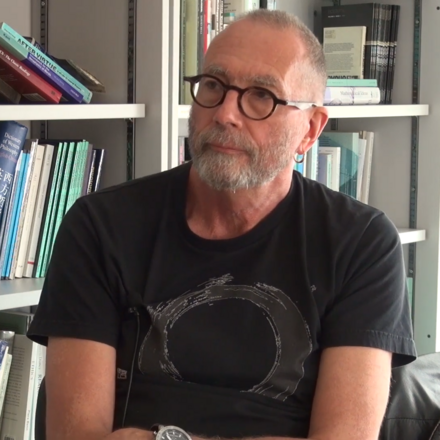
\includegraphics[width=0.6\textwidth]{priest.png}\\
    Graham Priest {\scriptsize\emph (Image by Wikipedia)}\\[3mm]
  \end{marginfigure}
Een voorbeeld van een dialetheia is \enquote{Deze zin is onwaar}. We kunnen deze zin als onwaar beschouwen, waardoor deze zou kloppen en dus tevens waar zou zijn. Als we deze zin als waar beschouwen, dan moeten we concluderen dat deze onwaar is. Een zin als deze wordt doorgaans als een paradox beschouwd en daarmee weggezet. Dialethe\"isme erkent het bestaan van dialetheia en probeert hier op een consistente manier meer te werken, waarbij verschillende paraconsistente logica's als formalisme gebruikt kunnen worden.
\end{aside}

\section{Modale Logica}\label{sec:modal}
Een modaliteit is een uitdrukking zoals \enquote{noodzakelijk} of \enquote{mogelijk}, die een waarheidswaarde kan be\"invloeden. In modale logica worden modaliteiten symbolisch binnen de logische taal weergegeven. Hiermee is modale logica, net als predicatenlogica, vooral een uitbreiding op een bestaand logisch systeem. Er bestaan verschillende modale logica's, elk met eigen interpetaties en axioma's. In de basis drukt modale logica noodzakelijkheid ($\Box A$, $A$ is noodzakelijk waar) en mogelijkheid ($\Diamond A$, $A$ is mogelijk waar), maar in deontische logica (die zich bezig houdt met ethische afwegingen) wordt dit bijvoorbeeld verplichting ($O$), toestaan ($P$) en verbod ($F$). Temporele logica (van \emph{tempus}, tijd) heeft het over ooit in het verleden ($P$), altijd in het verleden ($H$), ooit in de toekomst ($F$) en altijd in de toekomst ($G$). Doxastische logica gebruikt $BxA$ voor $x$ gelooft dat $A$, en Epistemische logica $KxA$ voor $x$ weet dat $A$; beide hebben toepassingen in game theory en bijvoorbeeld het raadsel van de \emph{muddy children}.

\begin{aside}[Muddy Children]
  Een groep kinderen\sidenote{... die allemaal kunnen redeneren en de basisprincipes van epistische logica kennen, zoals men zou verwachten ...} krijgt te horen dat tenminte een van hen modder op het gezicht heeft. Ieder kind kan het gezicht van alle anderen zien, maar niet van zichzelf, en mogen niet communiceren. Er wordt afgeteld, waarbij ieder kind dat weet dat het modder op het gezicht heeft gelijktijdig naar voren moet stappen. Als een kind foutief naar voren stapt wordt het gestrafd. Het proces herhaalt zich tot er alle kinderen met moddernaar voren zijn gestapt. Door zuiver redeneren kunnen de kinderen na een aantal iteraties zeker weten of ze wel of geen modder hebben; hoe?
\end{aside}

Wij zullen ons in deze sectie richten op de \enquote{basis}-variant van modale klassieke\sidenote{Het is mogelijk modaliteiten op verschillende logische systemen toe te passen; In de lineare logica is $\oc$ bijvoorbeeld ook een vorm van modaliteit. In de meeste gevallen waarin modale logica echte an sich bekeken wordt, is gebaseerd op een klassieke basis.} logica, die afhankelijk van gekozen aanvullende axioma's van verschillende interpretaties kan worden voorzien. We beperken ons daarmee tot de noodzakelijkheid $\Box$ en mogelijkheid $\Diamond$. Deze operatoren gedragen zich een beetje zoals respectievelijk $\forall$ en $\exists$, behalve dat ze geen variabele introduceren. Veel axioma's in de modale logica worden gedefinieerd aan de hand van $\Box$, waarbij $\Diamond$ kan worden gelezen als een notatie voor $\neg \Box \neg$ (iets dat noodzakelijk waar is, is onmogelijk onwaar).

De basis van het gros van de modale logica's is $\mathbf{K}$, dat naast de operatoren het axioma $\Box (A \to B) \to (\Box A \to \Box B)$ toevoegt (distributiviteit, ook wel axioma $K$). Daarnaast geldt voor elke $P$ dat $P$ een stelling in $\mathbf{K}$ is, dat $\Box P$ dit ook is.

Bovenop de modale logica $\mathbf{K}$ kunnen verdere axioma's toegevoegd worden. Een van de meest gebruikelijke is $\mathbf{T}$\sidenote{Soms ook bekend als $\mathbf{M}$.}, $\Box A \to A$. Als $A$ noodzakelijk waar is, dan is $A$ waar. Dit axioma wordt niet in elke vorm van modale logica's geaccepteerd --- in deontische logica zou dit vertalen naar $OA \to A$, en betekenen dat iedereen ook alles doet dat verplicht is; in temporale logica vertaalt dit naar $PA \to A$, alles dat altijd in het verleden het geval is geweest, is nu het geval (ook dit is, tot verdriet van veel Boomers, niet het geval).

Om semantiek te geven aan modale logica's wordt vaak gebruik gemaakt van een systeem van meerdere werkelijkheden, die met elkaar verbonden zijn. $\Box A$ betekent in dit geval dat $A$ waar is in alle werkelijkheden die met \enquote{onze} werkelijkheid\sidenote{De werkelijkheid van waaruit we redeneren.} onze werkelijkheid verbonden zijn, en $\Diamond A$ voor tenminste een van die werkelijkheden. Als twee werkelijkheden $w_0$ en $w_1$ met elkaar verbonden zijn, zodat modaliteiten in $w_0$ invloed hebben op $w_1$, dan schrijven we $w_0 > w_1$. Merk op dat nog nergens gesteld is dat onze werkelijkheid met zichzelf verbonden is, of dat die verbinding twee kanten op gaat. Binnen $\mathbf{K}$ geeft $\Box A$ aan dat in alle werkelijkheden die op de onze volgen, $A$ waar is, maar niet per definitie in onze eigen werkelijkheid. Dankzij het axioma $\mathbf{T}$ is dit in de gelijknamige logica $\mathbf{T}$ wel het geval en geldt $w_n > w_n$.

Een volgend axioma dat kan worden toegevoegd is $\mathbf{B}$: $A \to \Box \Diamond A$. Tezamen met $\mathbf{T}$ levert dit de logica $\mathbf{B}$ op. Het axioma stelt dat als $A$ waar is, dat dit in alle werkelijkheden die we kunnen bereiken mogelijk is, dus dat voor elk van deze werkelijkheden geldt dat we een werkelijkheid kunnen bereiken waar $A$ waar is. Deze werkelijkheid, die in alle richtingen 2 stappen van ons verwijderd is, is onze eigen werkelijkheid, wat betekent dat als we van werkelijkheid $w_0$ naar $w_1$ kunnen komen, we van $w_1$ weer terug in $w_0$ kunnen komen, oftewel $w_n > w_m \iff w_m > w_n$.

Alternatief kunnen we de axioma's $\mathbf{4}$ of $\mathbf{5}$ toevoegen aan $\mathbf{T}$ om met series modaliteiten om te gaan. $\mathbf{4}$ stelt $\Box A \to \Box \Box A$, en heeft tot gevolg dat we een serie gelijke modaliteiten tot \'e\'en kunnen samenvoegen\sidenote{Overtuig jezelf dat $\mathbf{4}$, die met $\Box$ gegeven is, voldoende is om deze uitspraak ook over $\Diamond$ te doen; gebruik hierbij de definitie van $\Diamond$ die eerder gegeven is.}. Concreet komt dit erop neer dat als $w_0 > w_1$ en $w_1 > w_2$, ook geldt dat $w_0 > w_2$. We mogen met dit axioma dus werkelijkheden overslaan. De logica met $\mathbf{K}$, $\mathbf{T}$ en $\mathbf{4}$ wordt $\mathbf{S4}$ genoemd. In plaats daarvan kunnen we ook axioma $\mathbf{5}$, $\Diamond A \to \Box \Diamond A$ , nemen om $\mathbf{S5}$ te krijgen. Hier kunnen we elke serie modaliteiten tot \'e\'en samenvoegen, en hoeven we allen de laatste te behouden. Als we $\mathbf{B}$ aan $\mathbf{S4}$ toevoegen krijgen we overigens precies dezelfde logica $\mathbf{S5}$.

De hier genoemde axioma's en systemen zijn de meest gangbare, maar zeker niet de enige modale systemen. De sequenten-regels overeenkomend met de axioma's staan gegeven in Stelling~\ref{th:sq-modal}.

\begin{figure}[ht]
\begin{theorem}\label{th:sq-modal} Regels voor modale logica
\mbox{}\\[3mm]
\inference{\Box_K}{\Gamma \vdash A}{\Box \Gamma \vdash \Box A}
\hspace{5mm}
\inference{\Box_T}{A, \Gamma \vdash \Delta}{\Box A, \Gamma \vdash \Delta} \\

\vspace{4mm}

\inference{\Box_4}{\Box \Gamma \vdash A}{\Box \Gamma \vdash \Box A}
\hspace{5mm}
\inference{\Box_5}{\Box \Gamma \vdash \Box \Delta, A}{\Box \Gamma \vdash \Box \Delta, \Box A}
\end{theorem}
\end{figure}

\chapter{Bewijsmethoden}\label{ch:bew:meth}
\begin{quote}
%The Final Proof of the non-Existence of God was proven by a Babel Fish.\\[2.5pt]
Now, [a Babel Fish\footnote{The Babel fish is small, yellow, leech-like - and probably the oddest thing in the universe. It feeds on brain wave energy, absorbing all unconscious frequencies and then excreting telepathically a matrix formed from the conscious frequencies and nerve signals picked up from the speech centres of the brain, the practical upshot of which is that if you stick one in your ear, you can instantly understand anything said to you in any form of language: the speech you hear decodes the brain wave matrix. \citep{adams}}] is such a bizarrely improbable coincidence that anything so mind-bogglingly useful could have evolved purely by chance that some have chosen to see it as the final proof of the NON-existence of God. The argument goes something like this:\\[2.5pt]
``I refuse to prove that I exist,'' says God, ``for proof denies faith, and without faith I am nothing.''\\[2.5pt]
``But,'' says Man, ``the Babel fish is a dead giveaway, isn't it? It could not have evolved by chance. It proves that You exist, and so therefore, by Your own arguments, You don't. QED.''\\[2.5pt]
``Oh dear,'' says God, ``I hadn't thought of that,'' and promptly vanishes in a puff of logic.\\[2.5pt]
``Oh, that was easy,'' says Man, and for an encore goes on to prove that black is white and gets himself killed on the next zebra crossing.
\end{quote}
\mbox{}\hfill\textit{Hitchhiker's Guide to the Galaxy -- \citet{adams}}\\[5pt]

{ \color{hured} Moet nog worden herzien.}

In verschillende delen van het ICT vakgebied is het wenselijk of noodzakelijk om gemaakte claims objectief en gedegen te onderbouwen, niet in de laatste plaats om anderen van de geldigheid ervan te kunnen overtuigen. Voor het geven van een onderbouwing van de geldigheid van een bewering is een heel scala van wiskundige bewijstechnieken en redeneervormen beschikbaar: \textit{bewijzen}. Voordat we deze technieken kunnen toepassen en op een generieke manier over problemen kunnen communiceren, is het in het algemeen noodzakelijk het probleem te modelleren in een formeel raamwerk: \textit{formaliseren}. Deze reader is er op gericht te oefenen met dit modelleren, en de vaardigheden op te doen in het toepassen van bewijstechnieken. 

\section{Waarom bewijzen?}
Teken eens een cirkel (of een aardappel, of iets wat daarop lijkt) met \'e\'en punt op de rand. De cirkel bestaat nu uit \'e\'en stuk. Teken nu een tweede punt op de rand, en verbind die met het eerste punt. Nu bestaat de cirkel uit twee stukken (zie ook Figuur \ref{fig:cirkel1}).
\begin{figure}
\begin{center}
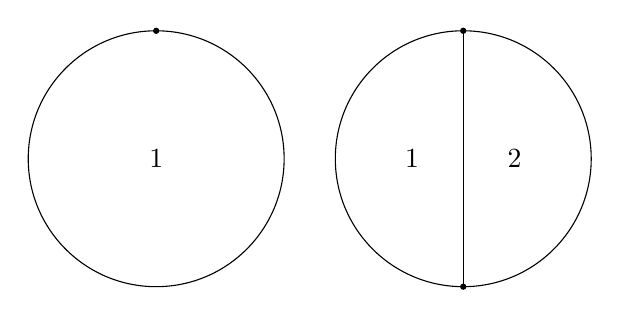
\begin{tikzpicture}[scale=.65]
\draw (3,3) circle (2.5cm);
\draw[fill=black] (3,5.5) circle (0.05cm);
\node at (3,3) {$1$};
\draw (9,3) circle (2.5cm);
\draw[fill=black] (9, 5.5) circle (0.05cm);
\draw[fill=black] (9, 0.5) circle (0.05cm);
\node at (8,3) {$1$};
\node at (10,3) {$2$};
\draw (9,5.5) -- (9,0.5);
\end{tikzpicture}
\end{center}
\caption{Cirkel met \'e\'en punt (links) en eentje met twee punten (rechts).}\label{fig:cirkel1}
\end{figure}

Teken nu een derde punt op de rand van de cirkel, en verbind die met de eerder gekozen punten. Nu bestaat de cirkel uit vier stukken. Teken ook nog een vierde punt, en verbind die weer met alle eerder gekozen punten. De cirkel bestaat nu uit acht stukken. Zie de plaatjes in Figuur \ref{fig:cirkel2}
\begin{figure}
\begin{center}
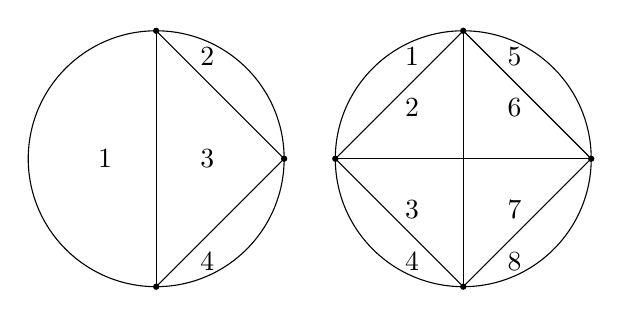
\begin{tikzpicture}[scale=.65]
\draw (3,3) circle (2.5cm);
\draw[fill=black] (3,5.5) circle (0.05cm);
\draw[fill=black] (3,0.5) circle (0.05cm);
\draw[fill=black] (5.5,3) circle (0.05cm);
\draw (3,5.5) -- (3,0.5);
\draw (3,5.5) -- (5.5,3);
\draw (5.5,3) -- (3,0.5);
\node at (2,3) {$1$};
\node at (4,5) {$2$};
\node at (4,3) {$3$};
\node at (4,1) {$4$};

\draw (9,3) circle (2.5cm);
\draw[fill=black] (9, 5.5) circle (0.05cm);
\draw[fill=black] (9, 0.5) circle (0.05cm);
\draw[fill=black] (11.5, 3) circle (0.05cm);
\draw[fill=black] (6.5, 3) circle (0.05cm);
\node at (8,1) {$4$};
\node at (8,2) {$3$};
\node at (8,4) {$2$};
\node at (8,5) {$1$};
\node at (10,1) {$8$};
\node at (10,2) {$7$};
\node at (10,4) {$6$};
\node at (10,5) {$5$};
\draw (9,5.5) -- (9,0.5);
\draw (9,5.5) -- (6.5,3);
\draw (6.5,3) -- (9,0.5);
\draw (9,0.5) -- (11.5,3);
\draw (11.5,3) -- (9,5.5);
\draw (6.5,3) -- (11.5,3);
\end{tikzpicture}
\end{center}
\caption{Cirkel met vier stukken (links); cirkel met acht stukken (rechts).}\label{fig:cirkel2}
\end{figure} 

We doen het nog een keer: we kiezen een vijfde punt en verbinden dat met de eerdere vier punten. Als we goed tellen zien we dat de cirkel nu in zestien stukken is opgedeeld. Er is hier duidelijk een patroon te zien: we beginnen met \'e\'en stuk, en elke keer als we een punt toevoegen en lijnen trekken krijgen we twee keer zo veel stukken. Bij \'e\'en punt hebben dus $2^0=1$ stukken, bij twee punten $2^1=2$, bij drie $2^2=4$ stukken, bij vier $2^3=8$ en bij vijf $2^4=16$ stukken. We concluderen nu:
\begin{quote}Als je $n$ punten op een cirkel met elkaar verbind, verdeel je daarmee de cirkel in $2^{n-1}$ stukken.\end{quote}

Dit klinkt allemaal best aannemelijk, en je bent niet zo gauw geneigd om dit nog verder uit te proberen voor zes of meer punten, want daarvoor met je toch al wel veel tekenen en tellen. Toch is het de moeite waard om dat wel eens te doen: bij zes punten lukt het je namelijk helemaal niet om $32$ stukken te krijgen, en blijft je bij $31$ stukken steken. Ook als je ervoor zorgt dat er nergens drie verbindingslijnen door \'e\'en punt gaan. We zijn er dus ingeluisd, en de hele bewering is niet waar (althans niet voor zes of meer punten).

De moraal van dit verhaal is dat als je echt zeker wilt weten dat een bewering waar is, je niet kunt vertrouwen op een paar voorbeelden en een aannemelijk verhaal dat een patroon in die voorbeelden verklaart. In de praktijk, zeker in die van de ICT, zijn er veel situaties waarin je geen genoegen kunt nemen met een paar testgevallen en een aannemelijk verhaal dat het wel goed zit. Durf je, bijvoorbeeld, te vliegen in een vliegtuig waarvan je zelf de besturingssoftware hebt geschreven, en best wel voor een redelijk aantal gevallen hebt uitgetest? Er zijn voldoende voorbeelden van dingen die fout gaan (met het verlies van mensenlevens tot gevolg) veroorzaakt door een foutje in de software \citep{fatalBugs}. Dit zijn toch dingen die je graag zou willen voorkomen.

Nu kun je niet verwachten dat je alle fouten kan voorkomen voor heel gecompliceerde dingen, maar een stap in die richting kan al heel waardevol zijn.  Wat je wilt hebben is een sluitende redenering dat een bepaalde bewering geldig is. Deze redenering kun je dan voor jezelf gebruiken, of om jezelf ervan te overtuigen dat je bewering geldig is. Maar je kunt diezelfde redenering ook gebruiken om iemand anders te overtuigen. Daarvoor is het nodig dat je de redenering opschrijft, en wel zodanig dat iemand anders aan de hand van wat je hebt opgeschreven de hele redenering ook kan volgen. En het liefst ook omgekeerd: alles wat je hebt opgeschreven speelt een essenti\"ele rol in de redenering. Zo'n redenering noemen we een \textit{bewijs}. De onderdelen van zo'n bewijs hebben een hele precieze betekenis. Een redenering met een heel precieze betekenis kun je alleen maar geven als alles wat je daarin zegt, inclusief de hele bewering waar het om gaat, heel precies is beschreven.

Vaak maak je bij het schrijven van redeneringen gebruik van manieren om je beweringen heel kort in een soort formule-taal op te schrijven, waarbij je een bijbehorende stel spelregels hebt. In dit dictaat zullen uitgebreid dergelijke notaties en begrippen aan de orde komen. Voordat we dat gaan doen lopen we eerst een aantal bewijsprincipes langs met bijbehorende voorbeelden, om een beetje een gevoel te ontwikkelen voor bewijsprincipes.

\section{Bewijzen uit het ongerijmde}\label{sec:pbc}
Bewering:
\begin{quote}
Een postbode levert $130$ poststukken af in een straat met $43$ adressen. Dan is er in die straat minstens \'e\'en adres waarop vier of meer poststukken worden afgeleverd.
\end{quote}
Hoe kun je nu het makkelijkste inzien dat deze bewering inderdaad klopt? Stel eens dat de geconcludeerde bewering (``er wordt op minstens \'e\'en adres vier of meer poststukken afgeleverd'') niet waar is. Dan worden er op elk adres dus hooguit drie poststukken afgeleverd. Met $43$ adressen in totaal betekent dat dat er in totaal hooguit $3\times 43=129$ poststukken worden afgeleverd. En dat is in tegenspraak met het gegeven dat er in totaal $130$ poststukken worden bezorgd. Dus de geconcludeerde bewering dat er minstens een adres is waarop vier of meer poststukken worden afgeleverd is wel waar, en we hebben zojuist deze bewering bewezen.

Het patroon in deze redenering komt heel vaak voor. Steeds is er een bewering waarvan je wilt bewijzen dat die waar is. De redenering zier dan als volgt uit:
\begin{quote}
Stel de bewering is niet waar. Vanuit de aanname trek je, eventueel samen met aannamen die deel uitmaken van de gegevens in de bewering, allerlei conclusies, tot je op een bewering uitkomt die niet waar is, of in tegenspraak is met gegevens in de bewering. Daaruit concludeer je dat de aanname 'de bewering is niet waar' niet kan kloppen, en daarmee is de bewering zelf wel waar.
\end{quote}

Een redenering van deze vorm wordt ook wel een bewijs uit het ongerijmde genoemd (in het Engels: proof by contradiction). In dit speciale voorbeeld wordt een telargument gegeven, dat ook wel het \textit{pigeon hole principle} (duiventilprincipe) wordt genoemd.

Als je van een bewering waarvan je denkt dat die waar is, probeert te bewijzen dat die inderdaad waar is, is het een goed idee om eens op een rijtje te zetten wat er allemaal gebeurt als die bewering niet waar is. Als het lukt om daar iets onzinnigs uit te concluderen, is de hele redenering om te vormen tot een bewijs uit het ongerijmde. 

Een waarschuwing is hier echter wel op zijn plaats: elke bewering die te bewijzen is, is op deze manier als volgt te bewijzen met een bewijs uit het ongerijmde. Stel de bewering is niet waar, geef een bewijs van de bewering, dit is in tegenspraak met de aanname dat de bewering niet waar is, en dus is de bewering waar. Wat betreft de geldigheid is hier niets tegenin te brengen, maar deze redenering bevat wel een hoop overbodige ballast: het bewijs van de bewering zelf is natuurlijk een stuk korter dan datzelfde bewijs met nog een hoop geredeneer er om heen. Uit het oogpunt van effici\"entie is een kort bewijs altijd te prefereren boven een langer bewijs. Tegen de tijd dat je een bewijs uit het ongerijmde hebt gevonden, is het dan ook altijd een goed principe om te kijken of je de redenering uit het ongerijmde wel echt nodig hebt, en niet in feite dezelfde redenering korter rechtstreeks kunt geven.

Nauw verwant aan een bewijs uit het ongerijmde is een bewijs met \textit{contrapositie}. Dat betekent dat je als een bewering van de vorm
\begin{quote}
Als $P$ geldt, dan geldt ook $Q$
\end{quote}
wilt bewijzen, in plaats hiervan ook mag bewijzen 
\begin{quote}
Als $Q$ niet geldt, dan geldt ook niet $P$.
\end{quote}

Merk op dat we twee keer het woord `niet' hebben toegevoegd, en $P$ en $Q$ hebben omgewisseld. We laten nu zien met een bewijs uit het ongerijmde dat dit nieuwe bewijsprincipe inderdaad klopt. We willen de bewering `Als $P$ geldt, dan geldt ook $Q$ bewijzen', en stellen dat dit niet  waar is. Dat  kan  alleen maar als er een  situatie bestaat waarin $P$ wel waar is, maar $Q$ niet; we  komen hier  later  uitgebreid  op  terug.  We  hadden  aangenomen dat we konden bewijzen `Als $Q$ niet geldt, dan geldt ook niet $P$'. Omdat in de  betreffende situatie $Q$ niet geldt, kunnen we dus concluderen dat dan ook $P$  niet geldt. Maar dit is in tegenspraak met de eerdere aanname dat in die situatie $P$ juist wel geldt.

Zoals gezegd is het een goed principe om van een bewering die je zou willen bewijzen, te gaan uitpluizen wat er allemaal gebeurt als die bewering niet waar is. Als het lukt om daar een tegenspraak uit af te leiden, is daarmee de bewering bewezen met een bewijs uit het ongerijmde. Als het echter niet lukt een tegenspraak te vinden, kun je juist gaan zoeken naar een voorbeeld waarvoor de bewering niet waar is. Als je zo’n voorbeeld hebt gevonden, heet dat een \textit{tegenvoorbeeld}, (Engels: \textit{counterexample}) waarmee dan juist bewezen is dat de bewering niet waar is.

\subsection{Opgaven}
\begin{exercise}[Optioneel]
Geef van elk van de volgende beweringen een bewijs of een tegenvoorbeeld:
\begin{itemize}
\item in elke groep van 50 mensen zijn er zes of meer die allemaal in dezelfde maand jarig zijn;
\item in elke groep van 50 mensen zijn er vijf of meer die allemaal in dezelfde maand jarig zijn;
\item in elke groep van 50 mensen zijn er vier of meer die allemaal in dezelfde maand jarig zijn.
\end{itemize}
\end{exercise}

\begin{exercise}[Optioneel]\label{ex:sqrt:2}
Rationale getallen zijn getallen die te schrijven zijn als $\frac{a}{b}$ voor willekeurige gehele $a$ en $b$ (d.w.z. $a,b \in \mathbb{Z}$).

Bewijs (uit het ongerijmde) dat de volgende bewering geldig is:
\begin{quote}
    Er is geen kleinste rationaal getal groter dan 0.
\end{quote}
\end{exercise}

\begin{exercise}[Optioneel]
Priemgetallen zijn natuurlijke getallen > 1 die slechts deelbaar zijn door 1 en zichzelf (bijv. 2, 3, 5, 7, 11, 13, 17, 19, 23, 29, \ldots).

Bewijs (uit het ongerijmde) dat de volgende bewering geldig is (ook wel bekend als de Stelling van Euclides):
\begin{quote}
    Er bestaat geen grootste priemgetal.
\end{quote}
\end{exercise}

\section{Bewijzen met gevalsonderscheiding}
Als je de getallen van 1 tot en met 100 bij elkaar optelt, wat komt er dan uit? Als je gaat rekenen: $1+2=3,3+3=6,6+4=10,10+5=15,\ldots$, dan ben je nog al even bezig. Het kan ook handiger:
$$1+100=101,2+99=101,3+98=101,\ldots,50+51=101$$
Nu hebben we de 100 getallen in 50 groepjes van twee opgesplitst, waarbij voor elk groepje van twee de som 101 is. Het totaal is dus $50\times 101=5050$.

Laten we het algemener bekijken (overigens ook een algemeen principe: probeer eerst een speciaal geval en als je daar iets voor verzonnen hebt, probeer dat dan algemener te maken). Als $k$ en $n$ gehele getallen zijn met $k<n$, en ik tel alle $n-k+1$ getallen van $k$ tot en met $n$ bij elkaar op, wat komt daar dan uit? Met hetzelfde trucje van zonet tellen we de eerste bij de laatste op, de op een na eerste bij de op een na laatste, en zo verder:
$$k+n=k+n,(k+1)+(n-1)=k+n,(k+2)+(n-2)=k+n,\ldots$$
Hoe eindigt dit? We zien dat het uitmaakt of het aantal $n-k+1$ even is of niet. Als dit aantal even is, krijgen we precies $\frac{n-k+1}{2}$ groepjes van twee waarvan de som steeds $k+n$ is. De som van de hele rij getallen is dus $(k+n)\times\frac{n-k+1}{2}=\frac{(k+n)(n-k+1)}{2}$.

Als het aantal oneven is, krijgen we $\frac{n-k}{2}$ groepjes van twee waarvan de som steeds $k+n$ is, en houden we het middelste element van de rij getallen over. Dat middelste getal is het gemiddelde van de eerste en de laatste, dus $\frac{k+n}{2}$. De som van al deze getallen is dus 
$$(k+n)\times\frac{n-k}{2}+\frac{k+n}{2}=\frac{(k+n)(n-k)+(k+n)}{2}=\frac{(k+n)(n-k+1)}{2}.$$
We zien dus dat ook in dit geval de som van de hele rij $\frac{(k+n)(n-k+1)}{2}$ is, en concluderen dat het in alle gevallen zo is. We hebben dus bewezen:
\begin{quote}
    Als $k$ en $n$ gehele getallen zijn met $k<n$, dan is de som van alle getallen van $k$ tot en met $n$ gelijk aan $\frac{(k+n)(n-k+1)}{2}$.
\end{quote}
In het bewijs van deze bewering hebben we een \textit{gevalsonderscheid} (Engels: \textit{case analysis}) gemaakt: voor het geval dat het aantal even was hebben we een bewijs gegeven, en voor het geval dat het aantal oneven was hebben we een ander bewijs gegeven. Aangezien elk geheel even of oneven is, hebben we hiermee voor alle gevallen een bewijs gegeven.

Net zoals bij bewijzen uit het ongerijmde is het bij bewijzen met gevalsonderscheid een goed principe om te kijken of je het gevalsonderscheid wel echt nodig hebt. Als je het namelijk niet nodig hebt, kun je waarschijnlijk een korter bewijs geven. In dit voorbeeld is dat inderdaad mogelijk als we met het maken van groepjes van twee niet stoppen als we op de helft zijn, maar nog even doorgaan:
$$k+n=k+n,(k+1)+(n-1)=k+n,(k+2)+(n-2)=k+n,\ldots$$
$$\ldots,(n-1)+(k+1)=k+n,n+k=k+n$$
Nu hebben we evenveel groepjes van twee gemaakt als het aantal getallen dat we bij elkaar op wilden tellen, namelijk $n-k+1$. Elk van deze groepjes heeft $k+n$ als som, al deze groepjes hebben dus samen $(k+n)(n-k+1)$ als som. In deze groepjes komen elk van de getallen precies twee keer voor: een keer als linkerlid van een groepje en een keer als rechterlid. Daarmee is tweemaal de gevraagde som dus gelijk aan $(k+n)(n-k+1)$, en concluderen we zonder gevalsonderscheid te maken dat de gevraagde som altijd gelijk aan $\frac{(k+n)(n-k+1)}{2}$.

In het eerste bewijs hebben we een opsplitsing in twee gevallen gemaakt: het aantal is even of het aantal is oneven. Het is ook mogelijk een probleem in meer dan twee gevallen op te splitsen. Van belang is altijd dat alle situaties die aan de voorwaarden van de bewering voldoen, onder tenminste een van de aangegeven gevallen vallen: de opsplitsing moet \textit{uitputtend} zijn, in het Engels: \textit{exhaustive}. Dat sommige situaties onder meer dan een van de gevallen vallen is niet erg. Dit illustreren we met het volgende voorbeeld:
\begin{quote}
    Voor elk re\"eel getal $x$ geldt dat $x\times x\geq 0$.
\end{quote}
We bewijzen dit als volgt: we maken het gevalsonderscheid $x\geq 0$ of $x\leq 0$. Dit onderscheid is inderdaad uitputtend: voor elk re\"eel getal $x$ geldt een van beide voorwaarden.

Als $x\geq 0$ dan is $x\times x$ het product van twee getallen die elk tenminste $0$ zijn; het product is dan ook tenminste 0.

Als $x\leq 0$ dan is $-x\geq 0$, en is $x\times x=(-x)\times(-x)$ het product van twee getallen die elk tenminste 0 zijn; het product is dan ook tenminste 0.

Voor beide gevallen hebben we nu een bewijs gegeven, en daarmee is het bewijs voltooid. Merk op dat het geval dat $x=0$ onder beide gevallen valt. In feite hebben we de bewering voor dit geval dus twee keer bewezen.

Het is een goed gebruik bij gevalsonderscheiding te beginnen bij de makkelijkste gevallen en het moeilijkste voor het laatst te bewaren.

\subsection{Opgaven}
\begin{exercise}[Optioneel]
Wat komt er uit als je alle even getallen van 2 tot en met 100 bij elkaar optelt? En wat komt er uit als je alle oneven getallen van 17 tot en met 47 bij elkaar optelt? Geeft een formule die voor elke $n$ aangeeft wat de som is van alle getallen van 2 tot en met $2n$.
\end{exercise}

\begin{exercise}[Optioneel]
Bewijs dat het kwadraat van een oneven getal altijd te schrijven is als $8n+1$ voor een geheel getal $n$.
\end{exercise}

\begin{exercise}[Optioneel]
Bewijs (met een gevalsonderscheid) de volgende stelling:
\begin{quote}
    Voor alle getallen $n\in\mathbb{Z}$ geldt $n^2 \text{ mod } 4 = 0\text{ of }1$.
\end{quote}
\end{exercise}
% We onderscheiden de volgende 2 gevallen:
% n is even: dan schrijven we n als 2m voor m ∈ Z. Nu geldt
% $n^2 = (2m)^2 = 4m^2$, en $4m^2/4 = m^2$ met rest 0.
% n is oneven: dan schrijven we n als 2m + 1 voor m ∈ Z. Nu geldt
% $n^2 = (2m + 1)^2 = 4m^2 + 4m + 1 = 4(m^2 + m) + 1$
% en $(4(m^2 + m) + 1)/4$ geeft rest 1.
% In beide gevallen hebben we rest 0 of 1.

\section{Bewijzen met inductie}
Voor beweringen die afhangen van een natuurlijk getal $n$ is het vaak handig om in het bewijs gebruik te maken van het gegeven dat de bewering voor kleinere waarden dan $n$ al waar is. Dat je daarmee toch een correct bewijs kunt leveren zegt het \textit{principe van volledige inductie}. In hoofdstuk \ref{ch:inductie} zal dit uitgebreid aan de orde komen.

\section{Bewijzen met invarianten}
\begin{remark}
De stof in deze sectie behoort niet tot de basisstof van het vak en zal niet getentamineerd worden. Ze is enkel toegevoegd voor ge\"interesseerde studenten die \textit{verder} willen dan de gemiddelde student.
\end{remark}
Alvorens het principe uit te leggen beginnen we met een aantal puzzels.

\subsection*{De keukenvloer}
We hebben een vierkante keukenvloer met een zijde van $n$ decimeter. In de rechteronderhoek en in de linkerbovenhoek mist een vierkante decimeter (voor een verwarmingsbuis). Voor welke $n$ kan de keukenvloer met tegels van $2\times 1$ decimeter betegeld worden? Bijvoorbeeld voor $n=6$ is de situatie als volgt:
\begin{center}
    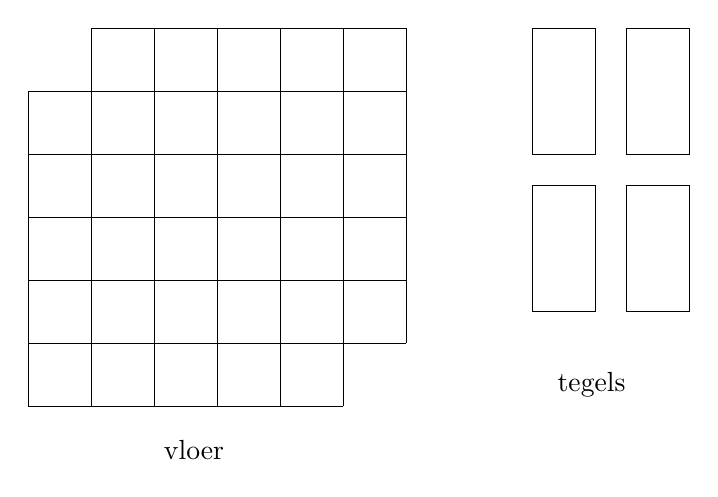
\begin{tikzpicture}[scale=.8]
    \draw[thin] (0,0) grid (5,5);
    \draw[thin] (-1,-1) grid (4,4);
    
    \draw[thin] (7, 0.5) rectangle (8,2.5);
    \draw[thin] (8.5, 0.5) rectangle (9.5, 2.5);
    \draw[thin] (7, 3) rectangle (8,5);
    \draw[thin] (8.5, 3) rectangle (9.5, 5);
    
    \node[anchor=south west] at (1,-2) {vloer};
    \node[anchor=south west] at (7.25, -1) {tegels};
    \end{tikzpicture}
\end{center}

\subsection*{De koffiekan}
In een koffiekan zitten 25 zwarte en 25 witte bonen. De volgende handeling wordt uitgevoerd zolang dat mogelijk is: \textit{haal twee bonen uit de kan; als ze dezelfde kleur hebben, stop dan een zwarte boon in de kan; als ze verschillend van kleur zijn, stop dan de witte boon terug in de kan}. Er is voldoende voorraad extra zwarte bonen. Vraag: wat is de kleur van de laatste boon in de kan?

\subsection*{De oplossingen}
Deze puzzels zijn allemaal gebaseerd op herhaling: herhaald tegels leggen en herhaald bonen trekken. Ze kunnen opgelost worden door steeds een geschikte \textit{invariant} te beschouwen, een eigenschap die steeds blijft gelden. We geven eerst de definitie.

\begin{definition}[Invariant]\mbox{}\\
Een invariant is een eigenschap van een proces of programma, die voldoet aan het volgende:
\begin{itemize}
    \item aan het begin geldt de invariant, en
    \item als de invariant geldt en er wordt vervolgens een stap gedaan, dan geldt na afloop van die stap de invariant weer.
\end{itemize}
\end{definition}

Als we zo'n eigenschap hebben, blijft die dus altijd gelden, hoeveel stappen er ook worden uitgevoerd. Als na eindig veel stappen het proces of programma voltooid is, geldt de invariant na afloop dus nog steeds. Deze observatie is cruciaal voor de oplossingen van elk van de puzzels, en is een belangrijk bewijsprincipe in de informatica.

\subsection*{Oplossing voor de keukenvloer}
We maken een gevalsonderscheid. Als $n$ oneven is dan is $n^2$ oneven, en $n^2-2$ dus ook. Een vloer van een oneven aantal dm$^2$ is nooit te betegelen met tegels die elk $2$ dm$^2$ groot zijn.

Als $n$ even is dan kleuren we de vloer in gedachten als een schaakbord: om en om wit en zwart, met de rechteronderhoek wit. De twee verwarmingsbuizen staan in een wit veld. Er moeten dus twee zwarte velden m\'e\'er betegeld worden dan witte velden. Omdat elke tegel \'e\'en zwart en \'e\'en wit veld bedekt, zullen we, hoe we ook tegelen, altijd twee zwarte velden overhouden. Een betegeling is dus niet mogelijk.

We hebben gebruik gemaakt van de invariant
$$\text{\it aantal onbetegelde zwarte velden = aantal onbetegelde witte velden + 2}$$
Deze uitspraak is in het begin waar, en blijft invariant bij het leggen van een tegel. De uitspraak geldt dus voor alle gedeeltelijke betegelingen, en er is geen betegeling waarin geen onbetegelde zwarte velden over zijn.

\subsection*{Oplossing voor de koffiekan}
Allereerst merken we op dat bij elke trekking er twee bonen verwijderd worden, en \'e\'en teruggelegd. Na 49 trekkingen zal er dus nog \'e\'en boon over zijn.

Het is ondoenlijk om alle mogelijkheden te proberen, dat zijn er heel erg veel. In plaats daarvan zoeken we naar een geschikte invariant. We kijken naar het netto effect op het aantal witte en zwarte bonen bij elk van de vier mogelijke trekkingen:
\begin{center}
    \begin{tabular}{|cc|cc|}
    \hline
    trekking & actie & $Z$ & $W$ \\
    \hline
    $-ZZ$ & $+Z$ & -1 & 0\\
    $-WW$ & $+Z$ & +1 & -2\\
    $-ZW$ & $+W$ & -1 & 0\\
    $-WZ$ & $+W$ & -1 & 0\\
    \hline
    \end{tabular}
\end{center}
Het witte aantal bonen in de kan blijft gelijk of neemt met twee af. Het oneven-zijn van het aantal witte is dus een invariant in dit spel!

Het aantal witte bonen blijft dus altijd oneven, in het bijzonder aan het eind. De laatste is dus altijd wit.

\subsection{Opgave}
\begin{exercise}[Optioneel]
In een doos zitten 100 rode, 100 witte en 100 blauwe ballen. Zolang dat mogelijk is, worden er drie ballen uit de doos gepakt. Als alle drie de ballen dezelfde kleur hebben, wordt er \'e\'en van die drie teruggelegd. Als alle drie de ballen een verschillende kleur hebben, wordt een rode bal teruggelegd. Als er twee ballen dezelfde kleur hebben, wordt de afwijkende derde teruggelegd en bovendien een blauwe. Is het mogelijk te eindigen met een rode en een blauwe bal?
\end{exercise}

\begin{exercise}[Optioneel]
Met de volgende regels kun je van rijtjes symbolen andere rijtjes symbolen maken:
\begin{enumerate}[label=\arabic*.]
    \item achter een rijtje met een $\mathsf{I}$ mag je een $\mathsf{U}$ zetten;
    \item van een rijtje $\mathsf{M}x$ mag je $\mathsf{M}xx$ maken, voor elk rijtje symbolen $x$;
    \item als er $\mathsf{I}\mathsf{I}\mathsf{I}$ in een rijtje staat, dan mag je dat vervangen door $\mathsf{U}$
    \item als er $\mathsf{U}\mathsf{U}$ in een rijtje staat, mag je dat weglaten.
\end{enumerate}
Als voorbeeld bekijken we een aantal rijtjes die je uit $\mathsf{MI}$ kunt produceren:

\begin{tabular}{lll}
a. & $\mathsf{MI}$ & gegeven \\
b. & $\mathsf{MII}$ & uit a volgens regel 2 \\
c. & $\mathsf{MIIII}$ & uit b volgens regel 2 \\
d. & $\mathsf{MIIIIU}$ & uit c volgens regel 1 \\
e. & $\mathsf{MUIU}$ & uit d volgens regel 3 \\
f. & $\mathsf{MUIUUIU}$ & uit e volgens regel 2 \\
g. & $\mathsf{MUIIU}$ & uit f volgens regel 4 
\end{tabular}

\noindent
Vraag: is het mogelijk om beginnend met het rijtje $\mathsf{MI}$ uit te komen op het rijtje $\mathsf{MU}$? Zo ja, hoe? Zo nee, waarom niet?\\
(Aanwijzing: laat zien dat in geen enkel opgebouwd rijtje het aantal $\mathsf{I}$'s een drievoud is.)
\end{exercise}

\chapter{Volledige Inductie}\label{ch:inductie}

In hoofdstuk \ref{sec:pred:semantiek} hebben we al lichtjes getipt aan de relatie tussen verzamelingenleer (hoofdstuk \ref{ch:verzamelingen}) en predikaatlogica (hoofdstuk \ref{ch:predicaten}). In dit hoofdstuk zullen we die relatie verder uitbouwen door het bespreken van een veel gebruikte bewijsstrategie, genaamd \textit{inductie}. Vooral voor oneindige domeinen, is bewijzen met inductie essentieel.

Inductieve definities, inductie en het daaraan gerelateerde concept van recursie vormen een krachtig hulpmiddel in informatica, logica, taalwetenschap en wiskunde. Het is mogelijk dit onderwerp -- zoals in de wiskunde gebruikelijk is -- binnen de Verzamelingenleer te ontwikkelen, maar omdat het echter direct inzichtelijk is (en volgens sommigen even fundamenteel als de Verzamelingenleer) introduceren wij het via een intu\"itive benadering. Het begin van alle dingen op dit gebied is de inductieve definitie. Inductieve definities zijn een middel om verzamelingen te cre\"eren. We beginnen met enkele voorbeelden.

\section{Inductieve definities}
In deze sectie voeren we inductieve definities in met behulp van voorbeelden. Inductieve definities geven ons een manier om met \textit{eindige} middelen \textit{oneindige} totaliteiten (verzamelingen) in te voeren.

\subsection*{Blurpsen}
We beginnen met de definitie van de verzameling der Blurpsen\footnote{Dit voorbeeld is ontleend aan Parvulae Logicales van \citet{parvulae}.}.
\begin{definition}
De verzameling van de Blurpsen is de kleinste verzameling zodat:
\begin{enumerate}[label=\roman*.]
    \item $\triangle$ is een Blurps.
    \item Als $x$ een Blurps is, dan zijn ook $x\triangle\triangle$ en $\Diamond xx\Diamond$ Blurpsen.
    \item Als $x$ en $y$ Blurpsen zijn, dan is ook $x\triangle y$ een Blurps.
\end{enumerate}
\end{definition}
Een inductieve definitie is een soort instructie om de elementen van de gedefinieerde verzameling te bouwen. Er is \'e\'en start element, te weten $\triangle$, op grond van clausule (i). In de context van onze definitie is $\triangle$ de atomaire Blurps. Uit $\triangle$ kunnen we op grond van (ii) de volgende elementen maken: $\triangle\triangle\triangle$ en $\Diamond\triangle\triangle\Diamond$. Op grond van (iii) kunnen we uit $\triangle$, $\triangle\triangle\triangle$ maken. Merk op dat we $\triangle\triangle\triangle$ dus op twee manieren kunnen produceren.

Uit de nieuwe gevormde Blurpsen kunnen we met (ii) en (iii) weer nieuwe Blurpsen maken:
$$\triangle\triangle\triangle\triangle\triangle, \Diamond\triangle\triangle\Diamond\triangle\triangle, \Diamond\triangle\triangle\triangle\triangle\triangle\triangle\Diamond,\Diamond\Diamond\triangle\triangle\Diamond\Diamond\triangle\triangle\Diamond\Diamond,$$
$$\triangle\triangle\triangle\triangle\triangle\triangle\triangle,\triangle\triangle\triangle\triangle\Diamond\triangle\triangle\Diamond, \Diamond\triangle\triangle\Diamond\triangle\triangle\triangle\triangle, \Diamond\triangle\triangle\Diamond\triangle\Diamond\triangle\triangle\Diamond.$$
Enzovoorts. De eerste zin van de definitie dat de gedefinieerde verzameling de kleinste is die aan de clausules voldoet, vertelt ons dat alleen maar dingen in de verzameling mogen worden gestopt op grond van het hierboven geschetste constructieproces. Zo kunnen bijvoorbeeld $\Diamond$ en $\Diamond\Diamond\Diamond\Diamond$ geen Blurpsen zijn. Deze eerste zin heet ook wel een \textit{minimaliteitsclausule}.

Bijvoorbeeld $\alpha:=\Diamond\Diamond\Diamond\Diamond$ is geen blurps om de volgende reden. Het is duidelijk dat $\alpha$ niet \'e\'en van der vormen $\triangle, x\triangle\triangle$, of $x\triangle y$ is. Dus als $\alpha$ een blurps was dan moet hij van de vorm $\Diamond xx\Diamond$ zijn, waar $x$ een blurps is. Maar $x$ kan niet van de vorm $\triangle, u\triangle\triangle$, of $u\triangle v$ zijn, omdat $\alpha$ geen $\triangle$ bevat. Ergo, $x$ is van de vorm $\Diamond yy\Diamond$. Dus $\alpha = \Diamond\Diamond yy\Diamond\Diamond yy\Diamond\Diamond$. Maar dan heeft $\alpha$ te veel $\Diamond$'s. Een tegenspraak met de aanname dat $\alpha$ een blurps is.

De tekens `$x$' en `$y$' die we in de definitie van de Blurpsen gebruikt hebben zijn niet zelf Blurpsen! Het zijn variabelen die wij gebruikten om over Blurpsen te spreken.

\begin{exercise}
Welke van de volgende rijtjes zijn Blurpsen:
$$\triangle\triangle\triangle\triangle, \triangle\triangle\triangle\triangle\triangle, \triangle\triangle\triangle\triangle\triangle\triangle, \triangle\triangle\triangle\triangle\triangle\triangle\triangle$$
$$\Diamond\Diamond\triangle\Diamond\Diamond\triangle\Diamond\Diamond\triangle\Diamond\Diamond, \Diamond\Diamond\Diamond\triangle\triangle\Diamond\Diamond\triangle\triangle\Diamond\Diamond\Diamond\triangle\triangle\Diamond\Diamond$$
\end{exercise}

\subsection*{Natuurlijke getallen}
We defini\"eren de natuurlijke getallen $\mathbb{N}$.
\begin{definition}
De verzameling der natuurlijke getallen is de kleinste verzameling zodat:
\begin{enumerate}[label=\roman*.]
    \item 0 is een natuurlijk getal.
    \item Als $x$ een natuurlijk getal is, dan is ook $x+1$ een natuurlijk getal.
\end{enumerate}
\end{definition}
Merk op dat we hier aannemen dat we al weten wat `$+1$' betekent. Ga na dat volgens onze definitie 0, 1, 2, 3, \ldots natuurlijke getallen zijn, maar niet: $-1, \frac{1}{2}, \pi$ en $i$. In onze nieuw verworven optiek is 0 het `atoom' van de natuurlijke getallen.

\subsection*{De taal $\mathcal{L}$ van de propositielogica}
We defini\"eren de taal van de propositielogica.
\begin{definition}
$\mathcal{L}$ is de kleinste verzameling zodat:
\begin{enumerate}[label=\roman*.]
    \item $p_o,p_1,p_2,p_3,\ldots$ zijn in $\mathcal{L}$.
    \item $\bot$ en $\top$ zijn in $\mathcal{L}$.
    \item Als $\varphi$ in $\mathcal{L}$ is, dan ook $\neg\varphi$.
    \item Als $\varphi$ en $\psi$ in $\mathcal{L}$ zijn, dan ook: $(\varphi\vee\psi), (\varphi\wedge\psi),(\varphi\rightarrow\psi),(\varphi\leftrightarrow\psi)$.
\end{enumerate}
\end{definition}
We gebruiken `$p$', `$q$', `$r$' als informele varianten van $p_0, p_1, p_2$. Bijvoorbeeld: $p$, $q$, $(p\wedge q)$, $r$, $\neg r$, $\neg\neg r$, $((p\wedge q)\rightarrow\neg\neg r)$ zijn in $\mathcal{L}$, maar $(($, $p\wedge q$, $)p\wedge q($ en $]$ zijn niet in $\mathcal{L}$.

De tekens `$\varphi$' en `$\psi$' die we in de definitie van $\mathcal{L}$ gebruikt hebben zijn niet zelf in $\mathcal{L}$. Ze zijn variabelen die we gebruiken in onze taal geheel analoog aan het gebruik van `$x$' en `$y$' bij de definitie van de Blurpsen. Merk op dat `$p_0$', `$p_1$', etc. ook wel \textit{propositievariabelen} genoemd worden. Zij zijn echter geen variabelen die wij als variabele gebruiken, maar objecten waarover we spreken, dit in tegenstelling tot `$\varphi$' en `$\psi$'. We noemen om het contrast te benadrukken `$\varphi$' en `$\psi$' soms \textit{metavariabelen}.

\subsection{Opgaven}
\begin{exercise}
Geef een inductieve definitie van de verzameling der natuurlijke getallen $n$ met $n\geq 5$.
\end{exercise}

\begin{exercise}
Maak een inductieve definitie van de verzameling van strings op alfabet $\{\mathtt{a},\mathtt{b}\}$ waarin de substring $\mathtt{bb}$ niet voorkomt.
\end{exercise}

\begin{exercise}
Maak een inductieve definitie van de verzameling van strings op alfabet $\{\mathtt{a},\mathtt{b}\}$ die er achterstevoren hetzelfde uitzien (z.g. palindromen, bijvoorbeeld `$\mathtt{abba}$').
\end{exercise}


\section{Inductie}
Bij elke inductief gedefinieerde verzameling hebben we de mogelijkheid eigenschappen van alle elementen van die verzameling te bewijzen met behulp van Volledige Inductie\footnote{Het ``Volledige'' in ``Volledige Inductie'' staat in contrast tot \textit{Onvolledige} of \textit{Enumeratieve} Inductie, de (ongeldige) redeneervorm waarin we uit het feit dat op de eerste drie daken een kat zit, concluderen dat op alle daken een kat zit. Omdat wij in dit dictaat alleen met Volledige Inductie van doen hebben, laten we het ``Volledige'' meestal weg.}. We geven voorbeelden van inductie over Blurpsen, van natuurlijke getallen en over $\mathcal{L}$.

\subsection*{Inductie over Blurpsen}
We bewijzen bijvoorbeeld: in elke Blurps komt een even aantal ruitjes voor.

Laten we eerst eens proberen dit op z'n janboerenfluitjes in te zien. Elke Blurps is gemaakt volgens de instructies. De eerste Blurps die je kunt maken is $\triangle$. $\triangle$ heeft 0 en dus een even aantal ruiten. Nu kunnen we bijvoorbeeld $\triangle\triangle\triangle$ maken, omdat we geen ruiten hebben toegevoegd, hebben we nog steeds 0 en dus een even aantal ruiten. We kunnen ook $\Diamond\triangle\triangle\Diamond$ maken, dit geeft ons 2 ruiten. Nu kunnen we weer $\Diamond\Diamond\triangle\triangle\Diamond\Diamond\triangle\triangle\Diamond\Diamond$ of $\Diamond\triangle\triangle\triangle\triangle\triangle\triangle\Diamond$ maken uit van $\Diamond\triangle\triangle\Diamond$ en $\triangle\triangle\triangle$. We hebben bij beiden 2 ruiten toegevoegd; bij de eerste we hadden er al twee ($\times$ twee), nu hebben we er dus zes. Verder experimenteren leert dat we niet in staat zijn een Blurps met oneven aantal ruiten te produceren, omdat je uit Blurpsen met een even aantal ruiten nooit Blurpsen met een oneven aantal ruiten kunt maken!

In detail gaat het zo: bij toepassing van de eerste helft van clausule (ii) voegen we geen ruiten toe, dus als het aantal al even was blijft het even.

Bij toepassing van de tweede helft van clausule (ii) maken we $\Diamond xx\Diamond$ uit $x$.
Als het aantal ruiten in $x$ even is, zeg $2n$, dan is het aantal ruiten in $\Diamond xx\Diamond$ gelijk aan $2n+2n+2$, met andere woorden $2(2n+1)$, een even aantal dus. 

Bij toepassing van clausule (iii) maken we $x\triangle y$ uit $x$ en $y$.
Als het aantal ruiten in $x$ even is, zeg $2n$, en als het aantal ruiten in $y$ even is, zeg $2m$, dan is het aantal ruiten in $x\triangle y$ gelijk aan $2n+2m$, dat is $2(n+m)$, een even aantal. 

Ons atoom $\triangle$ heeft een even aantal ruiten, de eigenschap `een even aantal ruiten hebben' plant zich voort over de toegelaten constructiestappen, dus alle Blurpsen hebben een even aantal ruiten.

Als we de minimaliteitsclausule in de definitie van Blurpsen hadden laten vallen, hadden we deze conclusie natuurlijk niet kunnen trekken: dan had $\Diamond\Diamond\Diamond$ best ook een Blurps kunnen zijn.

Bovenstaande redenering is in feite al een redenering met Volledige Inductie, we willen deze echter nog in `standaardvorm' zetten:

\noindent Laat het predikaat $P(x)$ uitdrukken dat `$x$ heeft een even aantal ruiten'. $P$ noemen we de Inductie Eigenschap.

We kunnen het te bewijzen nu als volgt herformuleren: te bewijzen is: voor alle Blurpsen $x$ geldt $P(x)$. De inductie verloopt nu in twee stadia: we controleren of $P$ opgaat voor de atomen en daarna laten we zien dat $P$ zich voortplant bij het maken van nieuwe Blurpsen volgens clausules (ii) en (iii). Dit laatste betekent dat we laten zien dat als $P$ opgaat voor de Blurpsen die we al gemaakt hebben, dat $P$ dan ook opgaat voor de uit de oude Blurpsen aangemaakte nieuwe Blurpsen.

De aanname dat $P$ opgaat voor al gemaakte Blurpsen noemen we de Inductie Hypothese (IH).

\noindent\begin{tabular}{lp{.84\textwidth}}
stap 1. & We hebben: $P(\triangle)$ (immers, $\triangle$ heeft een even aantal ruitjes, namelijk 0).\\
stap 2. & Stel $x$ is een Blurps met een even aantal ruiten (i.e., zodat $P(x)$; dit is de IH). Zeg het aantal ruiten in $x$ is $2n$. Dan heeft $x\triangle\triangle$ ook $2n$ ruiten, en dan heeft $\Diamond xx\Diamond$ $2\cdot 2n+2$ oftewel $2(2n+1)$ ruiten. Er volgt dat $P(x\triangle\triangle)$ en $P(\Diamond xx\Diamond)$.\\
stap 3. & Stel $x$ en $y$ zijn Blurpsen met een even aantal ruiten (IH). Zeg $x$ heeft $2n$ en $y$ heeft $2m$ ruiten. Dan heeft $x\triangle y$ $2n+2m$ oftewel $2(n+m)$ ruiten. Dus: $P(x\triangle y)$.
\end{tabular}\\
Met volledige inductie volgt nu: voor alle Blurpsen $x$ hebben we dat $P(x)$ geldt.

\begin{exercise}
Laat zien dat alle Blurpsen een oneven aantal driehoekjes hebben of tenminste \'e\'en ruit bevatten.
\end{exercise}

\subsection*{Inductie over natuurlijke getallen}
We laten zien dat voor alle natuurlijke getallen $x$ geldt:
$$0+1+\ldots +x=\frac{1}{2}\cdot x\cdot (x+1).$$
Zij $P(x) :=0+1+\ldots +x=\frac{1}{2}\cdot x\cdot (x+1)$.

\noindent\begin{tabular}{lp{.84\textwidth}}
stap 1. & Het is eenvoudig in te zien dat $P(0)$.\\
stap 2. & Stel $P(x)$ (IH). We hebben:
\begin{eqnarray*}
0+1+\ldots+x+(x+1) &=& \frac{1}{2}\cdot x\cdot(x+1)+(x+1)\\
&=&(\frac{1}{2}\cdot x+1)\cdot(x+1)\\
&=& \frac{1}{2}\cdot(x+2)\cdot(x+1)\\
&=& \frac{1}{2}\cdot(x+1)\cdot(x+2)
\end{eqnarray*}
Met andere woorden: $P(x+1)$.
\end{tabular}\\
We concluderen nu met Volledige Inductie: voor alle natuurlijke getallen $x$ geldt dat $P(x)$.

%\begin{exercise}[Optioneel]\mbox{}
%\begin{enumerate}[label=\arabic*.]
%    \item Laat zien dat $2^n>n^2$ voor alle $n\geq 5$.
%    \item Laat zien dat $1+2^2+\ldots+n^2=\frac{1}{6}n(n+1)(2n+1)$.
%\end{enumerate}
%\end{exercise}

\subsection*{Inductie over $\mathcal{L}$}
We laten zien dat formules $\varphi$ van $\mathcal{L}$ twee keer zoveel haakjes hebben als binaire logische voegtekens.

We defini\"eren de eigenschap $P(\varphi)$ als: $\varphi$ heeft twee keer zoveel haakjes als binaire logische voegtekens.

\noindent\begin{tabular}{lp{.84\textwidth}}
stap 1. & Als $\varphi$ een atoom is, is in $\varphi$ het aantal haakjes 0 en het aantal binaire logische voegtekens idem dito.\\
stap 2. & Stel $\varphi$ is van de vorm $\neg\psi$ en stel (IH): $P(\psi)$. We hebben: aantal haakjes in $\varphi =$ aantal haakjes in $\psi =$ twee keer het aantal binaire logische voegtekens in $\psi=$ twee keer aantal binaire voegtekens in $\varphi$.\\
stap 3. & Stel $\varphi$ is van de vorm $(\psi\wedge\chi)$ en stel (IH) $P(\psi)$ en $P(\chi)$. Zeg het aantal haakjes in $\varphi$, $\psi$, $\chi$ is respectievelijk $h_\varphi$, $h_\psi$ en $h_\chi$ en het aantal binaire logische voegtekens in $\varphi$, $\psi$, $\chi$ is respectievelijk $b_\varphi$, $b_\psi$ en $b_\chi$.\\
& We hebben
$$h_\varphi=h_\psi+h_\chi+2 = 2\cdot b_\psi+2\cdot b_\chi+2=2\cdot(b_\psi+b_\chi+1)=2\cdot b_\varphi.$$
De gevallen van $(\psi\vee\chi)$, $\psi\rightarrow\chi)$ en $(\psi\leftrightarrow\chi)$ zijn analoog.
\end{tabular}\\
Concludeer met volledige inductie dat voor alle $\varphi$ in $\mathcal{L}: P(\varphi)$.

\begin{exercise}\mbox{}
\begin{enumerate}[label=\arabic*.]
    \item Laat zien dat elke $\varphi$ in $\mathcal{L}$ evenveel linker- als rechterhaakjes heeft.
    \item Laat zien dat het aantal voorkomens van atomen in $\varphi$ in $\mathcal{L}$ groter of gelijk is aan het aantal linkerhaakjes in $\varphi$ plus 1.
\end{enumerate}
\end{exercise}

%\subsection*{Invarianten}
%%Jorn: wat is het doel van deze sectie. Het zegt nu  niks. De definitie van de invariant is dat het niet verandert, volgens wordt de definitie bewezen vanuit die definitie.
%%Wat je eigenlijk wil is bewijzen dat IETS een invariant IS.
%In hoofdstuk \ref{ch:inleiding} hebben we een aantal voorbeelden gezien van bewijzen met behulp van een \textit{invariant}. Zo'n invariant is een bepaalde eigenschap. Daarbij was de aanname dat
%\begin{itemize}
%    \item de invariant aan het begin geldt, en dat
%    \item als de invariant geldt en er wordt vervolgens een stap gedaan, dan geldt na afloop van die stap de invariant weer.
%\end{itemize}
%De conclusie die we dan trokken was dat de invariant na het uitvoeren van een willekeurig eindig aantal stappen altijd geldt. Destijds hebben we dat als principe geformuleerd en aannemelijk gemaakt; nu kunnen we de geldigheid van dit invariantenprincipe bewijzen met volledige inductie. We gaan met inductie naar $n$ bewijzen dat na $n$ de invariant geldig is. Voor $n=0$ geldt dit volgens de eerste aanname, daarmee is de basisstap bewezen. Vervolgens vragen we ons af of de invariant geldt na $n+1$ stappen. Het uitvoeren van $n+1$ stappen kunnen we zien als het uitvoeren van $n$ stappen en daarna nog \'e\'en stap. Volgens de inductiehypothese mogen we aannemen dat na $n$ stappen inderdaad de invariant geldt. Volgens de tweede aanname geldt dan dat na het uitvoeren van nog \'e\'en stap, dus na in totaal $n+1$ stappen, de invariant weer geldt. Volgens het principe van volledige inductie is hiermee bewezen dat voor elke $n$ geldt dat de invariant na uitvoeren van $n$ stappen geldt, precies wat we wilden bewijzen.

\subsection*{Torens van Hanoi}
De verschijningsvormen van inductie kunnen heel verschillend zijn. Het kan voorkomen dat inductie een handige methode is om iets te bewijzen wat slechts over \'e\'en specifiek getal $n$ gaat. Het kan makkelijker zijn om de algemene bewering voor elke willekeurige $n$ te bewijzen met inductie dan alleen maar de bewering over dat ene specifieke getal rechtstreeks te bewijzen. We gaan hier nu een voorbeeld van geven: de \textit{torens van Hanoi}.
\begin{center}
    \begin{tikzpicture}
    \draw (0,0) -- (9,0);
    \draw (1.4,1.75) rectangle (1.6, 3);
    \draw (0,0) rectangle (3,.25);
    \draw (.2,.25) rectangle (2.8,.5);
    \draw (.4, .5) rectangle (2.6, .75);
    \draw (.6,.75) rectangle (2.4, 1);
    \draw (.8, 1) rectangle (2.2, 1.25);
    \draw (1, 1.25) rectangle (2,1.5);
    \draw (1.2,1.5) rectangle (1.8,1.75);
    
    \draw (4.4,0) rectangle (4.6, 3);
    \draw (7.4,0) rectangle (7.6, 3);
    \end{tikzpicture}
\end{center}
Er zijn hier drie palen, en er zijn zeven schijven in oplopende grootte met een gat in het midden, die precies over de palen geschoven kunnen worden. In het begin liggen alle zeven schijven om de meest linkse paal, van onder naar boven gerangschikt van groot naar klein, zoals in het plaatje is aangegeven. De bedoeling is nu om deze hele stapel van schijven over te hevelen naar de middelste paal, zoals in het volgende plaatje is aangegeven:
\begin{center}
    \begin{tikzpicture}
    \draw (-3,0) -- (6,0);
    \draw (-1.4, 0) rectangle (-1.6, 3);
    \draw (1.4,1.75) rectangle (1.6, 3);
    \draw (0,0) rectangle (3,.25);
    \draw (.2,.25) rectangle (2.8,.5);
    \draw (.4, .5) rectangle (2.6, .75);
    \draw (.6,.75) rectangle (2.4, 1);
    \draw (.8, 1) rectangle (2.2, 1.25);
    \draw (1, 1.25) rectangle (2,1.5);
    \draw (1.2,1.5) rectangle (1.8,1.75);
    
    \draw (4.4,0) rectangle (4.6, 3);
    % \draw (7.4,0) rectangle (7.6, 3);
    \end{tikzpicture}
\end{center}
Hierbij moeten de volgende spelregels in acht worden genomen:
\begin{itemize}
    \item per stap kan er slechts \'e\'en schijf verplaatst worden, en wel de bovenste schijf van de stapel rond de ene paal naar een andere paal;
    \item een schijf mag nooit op een kleinere schijf worden gelegd.
\end{itemize}
De opdracht is nu om te laten zien dat:
\begin{itemize}
    \item je in 127 stappen de hele stapel rond de linkerpaal kunt overhevelen naar de middelste paal, en
    \item dat het niet in minder dan 127 stappen kan.
\end{itemize}
Hoewel deze opdracht betrekking heeft op de gegeven situatie met zeven schijven, ligt het voor de hand om eerst eenvoudigere instanties te bekijken met minder schijven. Hierbij volgen we een heel algemeen principe voor het aanpakken van een moeilijk probleem: probeer eerst eenvoudigere instanties van het probleem goed te begrijpen.

Laten we dus eens beginnen met \'e\'en schijf. Die kunnen we in \'e\'en stap van de linkerpaal naar de middelste paal overhevelen. Dat is wel erg makkelijk: na \'e\'en stap zijn we klaar. Ietsje lastiger wordt het met twee schijven. Als eerste stap moeten we dan de bovenste schijf van de linkerpaal naar de middelste of rechterpaal verplaatsen. Laten we de rechterpaal kiezen. Vervolgens kunnen we de onderste schijf van de linkerpaal naar de middelste paal  verplaatsen, en tenslotte kunnen we de kleinste schijf die we net rond de rechterpaal geparkeerd hebben naar het midden brengen, en zijn we klaar. Hier hebben we drie stappen voor nodig gehad. Als we nu gaan spelen met drie of vier schijven beginnen we het volgende patroon te ontdekken: als ik een stapel van $n$ van links naar het midden wil verplaatsen, moet ik eerst de bovenste $n-1$ naar de rechterpaal overhevelen, dan de onderste schijf naar het midden verplaatsen, en tenslotte de hele stapel van $n-1$ op de rechterpaal naar het midden overhevelen. Als ik het aantal stappen dat ik voor het verplaatsen van $n$ schijven nodig heb $f(n)$ noem, zie ik uit deze observatie dat $f(1)=1, f(2)=3, f(3)=7, f(4)=15, f(5)=31, f(6)=63,\ldots$ doet het patroon opdoemen dat $f(n)=2^n-1$. Op grond hiervan proberen we het volgende met inductie naar $n$ te bewijzen:
\begin{quote}
    Als we volgens bovenstaande spelregels een stapel van $n$ schrijven rond de linkerpaal willen overhevelen naar de middelste paal, kan dat in $2^n-1$ stappen, en kan het niet in minder dan $2^n-1$ stappen.
\end{quote}
\begin{proof}\mbox{}\\
\textbf{Basisstap:}\\
Voor $n=1$ kun je die ene schijf in $2^n-1=1$ stap naar het midden verplaatsen, en kan het niet in minder stappen. De bewering is dus waar voor $n=1$.\\[5pt]
\textbf{Inductiestap:}\\
We moeten twee dingen bewijzen: dat het kan in $2^n-1$ stappen, en dat het niet kan in minder dan $2^n-1$ stappen.\\
Dat het kan is als volgt in te zien.\\
Verplaats eerst de bovenste $n-1$ schijven van de linkerpaal naar de rechterpaal in $2^{n-1}-1$ stappen. Volgens de inductiehypothese\footnote{Merk op dat hoewel we hier $P(n-1)$ als inductiehypthese gebruiken om af te leiden dat $P(n)$, in plaats van $P(n)$ om $P(n+1)$ aan te tonen. Dit is uiteraard volledig analoog aan de hiervoorgaande bewijzen.} is een dergelijke verplaatsing mogelijk naar de middelste paal, maar door de rechterpaal en middelste paal elkaars rol in te laten nemen is dit ook mogelijk van de linkerpaal naar de rechterpaal. Vervolgens wordt de onderste schijf van links naar het midden verplaatst. Tenslotte worden de $n-1$ schijven van de rechterpaal naar de middelste paal verplaatst in $2^n-1$ stappen. Dit kan volgens de inductiehypothese door daarin de linkerpaal en de rechterpaal van rol te laten wisselen. Op deze wijze is de volledige stapel van $n$ schrijven van links naar het midden verplaatst: het hiervoor benodigde aantal stappen was $(2^{n-1}-1)+1+(2^{n-1}-1) = 2\cdot 2^{n-1}-1=2^n-1$.\\
We moeten nog laten zien dat het niet in minder stappen kan. Het is duidelijk dat de grootste schijf tenminste \'e\'en keer verplaatst zal moeten worden. Deze kan alleen maar verplaatst worden volgens de spelregels als alle andere schijven rond de paal geplaatst zijn waar de grootste schijf niet vandaan komt en ook niet naar toe gaat. Volgens de inductiehypothese zijn voor het verplaatsen van de andere $n-1$ schijven naar een andere paal tenminste $2^{n-1}-1$ stappen nodig. Tenslotte zal na de laatste keer dat de grootste schijf verplaatst wordt, de hele stapel van $n-1$ kleinere weer naar het midden moeten worden overgeheveld. Ook hier zijn volgens de inductiehypothese tenminste $2^{n-1}-1$ stappen nodig. In totaal is het minste aantal hiervoor benodigde stappen dus $(2^{n-1}-1)+1+(2^{n-1}-1)=2^n-1$.
\end{proof}

Het oorspronkelijke probleem voor zeven schijven is nu opgelost door deze bewering die we net hebben bewezen voor elke $n\geq 1$, toe te passen voor $n=7$.

Het is zelfs met deze redenering in te zien dat het verplaatsen van de hele stapel van $n$ schijven van de linkerpaal naar de middelste paal slechts op precies \'e\'en manier kan in $2^n-1$ stappen, en wel volgens de manier die in het bewijs is aangegeven en eenvoudig in een algoritme kan worden omgezet.

\subsection{Opgaven}
\begin{exercise}[Optioneel]
Een spel begint met $n>1$ pionnen. Vooraf wordt een getal $m$ vastgesteld met $1\leq m<n$. Spelers $A$ en $B$ gooien om beurten hoogstens $m$ pionnen om (telkens minimaal 1 pion). Winnaar is degene die de laatste pion(nen) omgooit. Bewijs dat de beginner kan winnen, dan en slechts dan als $n$ geen veelvoud van $m$ is.
\end{exercise}

\begin{exercise}[Optioneel]
Een spel wordt gespeeld met twee stapels fiches, $n_1$ fiches op de ene stapel en $n_2$ fiches op de andere stapel. Spelers $A$ en $B$ mogen om beurten fiches van \'e\'en van de stapels pakken, minstens 1 en maximaal alle fiches van een stapel. Winnaar is die de laatste fiches pakt.

Bewijs: de beginner kan winnen dan en slechts dan als $n_1\not =n_2$.\\
Aanwijzing: inductie naar $n_1+n_2$.
\end{exercise}

\begin{exercise}[Optioneel]
Beschouw voor een natuurlijk getal $n\geq 1$ de uitspraak:

\noindent $P(n):=$ in elke groep van $n$ meisjes hebben alle meisjes even lang haar.

Als we om ons heen kijken, zien we dat $P(n)$ niet waar is. Waar zit dus de fout in het volgende bewijs van $P(n)$ voor alle $n\geq 1$:

\noindent\begin{tabular}{lp{.84\textwidth}}
stap 1. & $P(1)$, want dan bestaat de groep maar uit 1 meisje.\\
stap 2. & Stel $P(x)$ en neem een groep van $x+1$ meisjes. Stuur een van de meisjes, zeg Sandra, even uit de groep. De overige meisjes vormen een groep van $x$ meisjes, en hebben dus even lang haar (IH). Haal nu Sandra terug in de groep, en stuur een ander meisje uit de groep. Weer hebben we nu een groep van $x$ meisjes, waaronder Sandra. Sandra heeft dus even lang haar als de andere meisjes. Dus in de complete groep van $x+1$ meisjes hebben alle meisjes even lang haar: $P(x+1)$
\end{tabular}
\end{exercise}


\chapter{Functies}\label{app:functies}
In sectie \ref{sec:functies} hebben we al kort kennis gemaakt met het concept \textit{functie}. In dit hoofdstuk zullen we dit nog wat verder uitdiepen.

\section{Inversen}
%Wanneer we voor twee verzamelingen $A$ en $B$ bij elk element van $A$ precies \'e\'en element van $B$ vastleggen, dan hebben we een \textit{afbeelding} van $A$ naar $B$ gedefinieerd. In plaats van afbeelding zegt men ook wel \textit{functie}. In het Engels heet een afbeelding een \textit{map} of \textit{function}.
%
%Door middel van een afbeelding van $A$ naar $B$ wijst elk element van $A$ dus een element van $B$ aan. Een element van $B$ kan vaker aangewezen worden. Een element van $A$ kan niet meer dan \'e\'en element van $B$ aanwijzen. Wij zullen ons meestal bedienen van deze terminologie van aanwijzen. Dit komt ook overeen met de veelgebruikte manier om een afbeelding van $A$ naar $B$ te visualiseren door middel van een tekening waarin vanuit elk punt van een getekende verzameling $A$ een pijl vertrekt die aankomt in een van de punten van de getekende verzameling $B$.
%\begin{center}
%\begin{tikzpicture}
%\draw[rounded corners=25pt] (0,0) rectangle (2,3);
%\draw[rounded corners=25pt] (4,0) rectangle (6,3);
%\draw[fill] (1.25, .5) circle (.05cm) node (a1) {};
%\draw[fill] (1.3, 1) circle (.05cm) node (a2) {};
%\draw[fill] (0.5, 1.2) circle (.05cm) node (a3) {};
%\draw[fill] (0.6, 1.8) circle (.05cm) node (a4) {};
%\draw[fill] (0.8, 2.3) circle (.05cm) node (a5) {};
%\draw[fill] (4.7, .5) circle (.05cm) node (b1) {};
%\draw[fill] (5.6, .7) circle (.05cm) node (b2) {};
%\draw[fill] (4.6, 1.5) circle (.05cm) node (b3) {};
%\draw[fill] (5.5, 1.4) circle (.05cm) node (b4) {};
%\draw[fill] (5.7, 2.0) circle (.05cm) node (b5) {};
%\draw[fill] (5.1, 2.5) circle (.05cm) node (b6) {};
%
%\draw[->] (a1) -- (b1);
%\draw[->] (a2) -- (b5);
%\draw[->] (a3) -- (b6);
%\draw[->] (a4) -- (b2);
%\draw[->] (a5) -- (b1);
%\end{tikzpicture}
%\end{center}
%
%Zo'n plaatje heet ook wel een \textit{pijlendiagram}.
%
%Een afbeelding bestaat dus uit een drietal: een verzameling $A$, een verzameling $B$, en een beschrijving die aangeeft hoe de aanwijzing van elementen van $B$ door de elementen van $A$ er uitziet.
%
%Korten we die beschrijving af door een letter, bijvoorbeeld $f$, dan is de afbeelding dus het drietal $(A, B, f)$.
%$$A\text{ heet het \textit{domein} van }f\text{ (Engels: \textit{domain}),}\\$$
%$$B\text{ heet het \textit{bereik} van }f\text{ (Engels: \textit{range}).}$$
%
%Een suggestieve en zeer vaak gebruikte notatie is
%$$f: A\rightarrow B.$$
%Alhoewel de pijl hier verward zou kunnen worden met de logische pijl, staat de context er vrijwel altijd borg voor dat dit niet gebeurt. De combinatie $A\rightarrow B$ van domein en bereik heet wel het \textit{type} van de afbeelding $f$.
%
%Is $x$ een element van $A$, dan duidt $f(x)$ het \textit{beeld} van $x$ aan (Engels: \textit{image}), het element van $B$ dat door $x$ wordt aangewezen. Het element $x$ heeft dan wel het \textit{argument} van de afbeelding.
%
%Twee afbeeldingen $f:A\rightarrow B$ en $g:C\rightarrow D$ zijn aan elkaar \textit{gelijk} (en dus dezelfde afbeelding), precies dan als aan drie voorwaarden voldaan is:
%\begin{enumerate}
%    \item $A = C$;
%    \item $B = D$;
%    \item voor alle $x\in A$ geldt dat $f(x) = g(x)$.
%\end{enumerate}
%\begin{example}
%Enkele voorbeelden van afbeeldingen zijn:
%\begin{itemize}
%    \item $A=\mathbb{R}, B=\mathbb{R},$ voor alle $x\in\mathbb{R}$ is $f(x)=\text{sin}(x)$;
%    \item $A=\{1, 2, 3\}, B=\{a, b, c, d\}, f(1)= b, f(2) = d, f(3) = b$;
%    \item $A=\mathbb{N}, B=\{2,3,5,6\},$ voor alle $n\in\mathbb{N}$ is $f(n)=5$.
%\end{itemize}
%In het vervolg zullen we het tweede voorbeeld nog een aantal keren aanhalen. Enkele gevallen waarin we niet met een afbeelding van doen hebben, zijn:
%\begin{itemize}
%    \item $A=\mathbb{R}, B=\mathbb{R}, f(x)=\text{ln}(x)$,\\ want $\text{ln}(x)$ is niet voor elke $x\in\mathbb{R}$ gedefinieerd.
%    \item $A=\mathbb{N}, B=\mathbb{Q}, f(x)=\sqrt{x}$,\\ want $\sqrt{2}\not\in\mathbb{Q}$.
%\end{itemize}\label{vb:func}
%\end{example}
%
%Bij een afbeelding $f:A\rightarrow B$ en een deelverzameling $X$ van $A$ kunnen we kijken naar de deelverzameling van $B$ bestaande uit de beelden van alle elementen van $X$. Deze deelverzameling van $B$ heeft het \textit{beeld} van $X$, en wordt aangeduid met $f(X)$.
%$$f(X) = \{y\in B\;|\;\text{er is een } x\in X(y=f(x))\}$$
%Merk op dat zowel de notatie als de terminologie hiervan overeenkomt met het beeld van een element. Uit de context moet dus worden opgemaakt om welk van de twee begrippen het gaat: als $x$ een element is van $A$ dan is $f(x)$ het bijbehorende element van $B$; als $x$ een deelverzameling is van $A$ dan is $f(x)$ de deelverzameling van $B$ bestaande uit bij die deelverzameling horende elementen van $B$.

In het voorbeeld van \ref{vb:func} hebben we onder andere
$$f(\{1\})=\{b\}, f(\{1,2\})=\{b,d\}, f(\{1,3\})=\{b\},f(A)=\{b,d\}$$

De verzameling $f(A)$ wordt wel het \textit{beeld} van $f$ genoemd. Ook kunnen we bij een deelverzameling $Y$ van $B$ vragen naar de deelverzameling van $A$ bestaande uit alle $x$ waarvoor $f(x)\in Y$. Deze deelverzameling heet het \textit{volledig origineel} (Engels: \textit{inverse image}) van $Y$, en wordt aangeduid met $f^{-1}(Y)$.
$$f^{-1}(Y)=\{x\in A\;|\; f(x)\in Y\}.$$

We kijken weer naar ons eerdere voorbeeld \ref{vb:func}, hier geldt:\\[1.5pt]
\begin{tabular}{llll}
$f^{-1}(\{a\})=\varnothing$,&$f^{-1}(\{c\})=\varnothing$,&$f^{-1}(\{a,b\})=\{1,3\}$,&$f^{-1}(\{a,d\})=\{2\}$,\\
$f^{-1}(\{b\})=\{1,3\}$,&$f^{-1}(\{d\})=\{2\}$,&$f^{-1}(\{a,c\})=\varnothing$,&$f^{-1}(\{b,d\})=A$
\end{tabular}\\[1.5pt]

Wanneer de deelverzameling $Y$ van $B$ bestaat uit slechts \'e\'en element, schrijft men gewoonlijk $f^{-1}(y)$ in plaats van $f^{-1}(\{y\})$. Dus:
\begin{itemize}
    \item als $x$ een element is van $A$ dan is $f(x)$ een element van $B$;
    \item als $X$ een deelverzameling is van $A$ dan is $f(X)$ een deelverzameling van $B$;
    \item als $y$ een element is van $B$ dan is $f^{-1}(y)$ een deelverzameling van $A$;
    \item als $Y$ een deelverzameling is van $B$ dan is $f^{-1}(Y)$ een deelverzameling van $A$.
\end{itemize}

Een speciale situatie ontstaat als we voor een deelverzameling $X$ van $A$ kijken naar het volledige origineel van het beeld van $X$, of als we voor een deelverzameling $Y$ van $B$ kijken naar het beeld van het volledig origineel van $Y$.
\begin{theorem}\label{st:afb}
Zij $f:A\rightarrow B$ een afbeelding. Dan gelden:
\begin{enumerate}
    \item $f^{-1}(B)=A$
    \item Als $X\subseteq A$, dan $X\subseteq f^{-1}(f(X))$
    \item Als $Y\subseteq B$, dan $f(f^{-1}(Y))\subseteq Y$
\end{enumerate}
\end{theorem}
\begin{proof}\mbox{}\\

\begin{minipage}{.9\textwidth}
Bewijs van (1):\\[1.5pt]
Kies $x\in f^{-1}(B)$ willekeurig. Dan geldt $x\in A$. Dus $f^{-1}(B)\subseteq A$.\\[1.5pt]
Kies omgekeerd $x\in A$ willekeurig. Dan $f(x)\in B$, dus $x\in f^{-1}(B)$. Dus $A\subseteq f^{-1}(B)$.\\[1.5pt]
Met beide resultaten samen hebben we $f^{-1}(B)=A$.\hfill$\fbox{1}$\\[2.5pt]
Bewijs van (2):\\[1.5pt]
Kies $x\in X$ willekeurig. Dan $f(x)\in f(X)$. dus $x\in\{x\in A\;|\;f(x)\in f(X)\} = f^{-1}(f(X))$. Dus $X\subseteq f^{-1}(f(X))$.\hfill$\fbox{2}$\\[2.5pt]
Bewijs van (3):\\[1.5pt]
Kies $z\in f(f^{-1}(Y))$ willekeurig. Dan is er een $x\in f^{-1}(Y)$ met $z=f(x)$. Vanwege $x\in f^{-1}(Y)$ geldt $f(x)\in Y$. Vanwege $z=f(x)$ geldt $z\in Y$. Vanwege $z=f(x)$ geldt $z\in Y$. Hiermee is bewezen $f(f^{-1}(Y))\subseteq Y$.\\ \mbox{}\hfill$\fbox{3}$
\end{minipage}\\
\end{proof}

Een zeer vaak gemaakte fout is om te menen dat:
$$f(f^{-1}(Y)) = Y\text{ en dat } f^{-1}(f(X)) = X.$$
Dat dit niet waar is illustreren we met behulp van ons eerdere voorbeeld \ref{vb:func}: daarin geldt
$$f(f^{-1}(\{a,d\})) = f(\{2\}) = \{d\}\not = \{a,d\}$$
en
$$f^{-1}(f\{1\})) = \{1, 3\}\not=\{1\}.$$

\section{Injectieve, surjectieve en bijectieve afbeeldingen}
Vaak bekijkt men afbeeldingen $f:A\rightarrow B$ die aan speciale wensen voldoen. We laten een drietal van zulke extra eisen de revue passeren.

Een afbeelding $f:A\rightarrow B$ heet \textit{injectief} als geen twee verschillende elementen van $A$ eenzelfde element van $B$ aanwijzen, dus als voor elk element $z\in B$ bestaat $f^{-1}(z)$ uit hoogstens \'e\'en element.

Een injectieve afbeelding heet ook wel een \textit{injectie}.

Als je wilt bewijzen dat $f:A\rightarrow B$ injectief is, kies je willekeurig twee elementen $x,y \in A$ waarvoor je aanneemt dat $f(x)=f(y)$. Als je dan kunt bewijzen dat $x=y$, heb je volgens deductie bewezen dat $f$ injectief is.

Als je daarentegen twee verschillende elementen $x,y\in A$ kunt vinden waarvoor geldt dat $f(x)=f(y)$, dan heb je daarmee juist bewezen dat $f:A\rightarrow B$ niet injectief is (door middel van een \textit{tegenvoorbeeld}).

Een afbeelding $f:A\rightarrow B$ heet \textit{surjectief} als elk element van $B$ optreedt als beeld, dus als voor elk element $z\in B$ de functie $f^{-1}(z)$ uit minstens \'e\'en element. Nog korter gezegd: $f(A)=B$.

Een surjectieve afbeelding heet ook wel een \textit{surjectie}.

Als je wilt bewijzen dat $f:A\rightarrow B$ surjectief is, kies je een willekeurig element $z\in B$. Als je daarvoor een element $x\in A$ kunt vinden waarvoor geldt $f(x)=z$ heb je bewezen dat $f$ surjectief is.

Als je een element $x\in B$ kunt vinden dat voor geen enkel element $x\in A$ te schrijven is als $z=f(x)$, dan heb je daarmee juist bewezen dat $f$ niet surjectief is.

Een afbeelding $f:A\rightarrow B$ heet \textit{bijectief} als hij injectief en surjectief is. Dus als elk element van $B$ optreedt als beeld van precies \'e\'en element van $A$. Preciezer gezegd: voor elk element $z\in B$ bestaat $f^{-1}(z)$ uit precies \'e\'en element.

Een bijectieve afbeelding heet ook wel een \textit{bijectie}.

Als voorbeeld beschouwen we de afbeelding $s:\mathbb{N}\rightarrow\mathbb{N}$ gedefinieerd door $s(x)=x+1$ voor alle $x\in\mathbb{N}$. Deze afbeelding heet de \textit{successor}.

Deze afbeelding is injectief, want uit $s(x)=s(y)$ concluderen we dat $x+1=y+1$ en daaruit volgt dat $x=y$.

Deze afbeelding is niet surjectief, want voor $0\in\mathbb{N}$ bestaat er geen $x\in\mathbb{N}$ waarvoor geldt $s(x)=0$.

Omdat de afbeelding $s$ niet surjectief is, is $s$ ook niet bijectief.

Het voorbeeld van \ref{vb:func} is niet injectief, want daar geldt $f(1)=b=f(3)$. Tevens is ze ook niet surjectief, want de elementen $a$ en $c$ treden niet op als beeld van $f$.

Intu\"itief betekent injectiviteit dat er bij het toepassen van de afbeelding geen informatie verloren gaat. In de informatica is dit bijvoorbeeld essentieel bij \textit{datacompressie}: je wilt een file in minder geheugen opslaan dan hij zelf beslaat, maar wel zodanig dat de oorspronkelijke file exact te reconstrueren valt uit de gecomprimeerde versie. In feite heb je hier met een afbeelding te maken: datacompressie is het toepassen van een afbeelding op een file. Zowel het domein als het bereik van deze afbeelding is de verzameling van alle mogelijke files. Deze afbeelding is bruikbaar als datacompressie als voor grote files van een veelvoorkomend type geldt dat hun beeld onder deze afbeelding (aanzienlijk) kleiner is. Maar heel essentieel is ook dat er een \textit{decompressie}-afbeelding bestaat die de oorspronkelijke file exact reconstrueert. Als de afbeelding $f$ die de datacompressie beschrijft niet injectief is zal dit nooit lukken. Dan bestaan er namelijk verschillende files $x$ en $y$ met $f(x)=f(y)$. Aan de hand van de gecomprimeerde versie $f(x)=f(y)$ is het dan onmogelijk vast te stellen of de oorspronkelijke file nou $x$ is of $y$, of misschien nog wel wat anders.

Precies hetzelfde speelt bij \textit{encryptie}: je wilt een boodschap zodanig versleutelen dat hij voor buitenstaanders niet toegankelijk is. De rechtmatige ontvanger beschikt over een \textit{sleutel} waarmee de oorspronkelijke boodschap weer uit de versleutelde versie te reconstrueren is. Om precies dezelfde reden als hierboven kan dat alleen als de versleutelingsafbeelding injectief is. 

In stelling \ref{st:afb} hebben we twee inclusies gezien die in het algemeen geen gelijkheden waren ($f(f^{-1}(Y))=Y$ en $f^{-1}(f(X))=X$). We laten nu zien dat ze dat wel zijn als de betreffende afbeeldingen respectievelijk injectief en surjectief zijn.
\begin{theorem}\label{th:injectief}
Als $f:A\rightarrow B$ een injectieve afbeelding is, en $X$ een deelverzameling van $A$, dan is $f^{-1}(f(X))=X$.
\end{theorem}
\begin{proof}\mbox{}\\
\indent\begin{minipage}{0.9\textwidth}
In Stelling \ref{st:afb} hebben we al bewezen dat $X\subseteq f^{-1}(f(X))$; we hoeven nu alleen nog te bewijzen dat $f^{-1}(f(X))\subseteq X$.\\[1.5pt]
Kies daartoe $x\in f^{-1}(f(X))$ willekeurig.\\[1.5pt]
Volgens de definitie van $f^{-1}$ geldt dan $f(x)\in f(X)$.\\[1.5pt]
Volgens de definitie van $f(X)$ is er dan een $y\in X$ met $f(x)=f(y)$.\\[1.5pt]
Omdat $f$ injectief is geldt dan $x=y$.\\[1.5pt]
Omdat $y\in X$ is hiermee bewezen dat $x\in X$.\\[1.5pt]
Hiermee is bewezen dan $f^{-1}(f(X))\subseteq X$.
\end{minipage}\\
\end{proof}
\begin{theorem}\label{th:surjectief}
Als $f:A\rightarrow B$ een surjectieve afbeelding is, en $Y$ een deelverzameling van $B$ is, dan is $f(f^{-1}(Y))=Y$.
\end{theorem}
\begin{proof}\mbox{}\\
\indent\begin{minipage}{0.9\textwidth}
In Stelling \ref{st:afb} hebben we al bewezen dat $f(f^{-1}(Y))\subseteq Y$; we hoeven nu alleen nog te bewijzen dat $Y\subseteq f(f^{-1}(Y))$.\\[1.5pt]
Kies daartoe $y\in Y$ willekeurig.\\[1.5pt]
Omdat ook $y\in B$ en $f$ surjectief is, is er een $x\in A$ met $f(x)=y$.\\[1.5pt]
Volgens de definitie van $f^{-1}$ geldt dan $x\in f^{-1}(Y)$.\\[1.5pt]
Daaruit volgt dat $f(x)\in f(f^{-1}(Y))$.\\[1.5pt]
Omdat $f(x) = y$ geldt nu $y\in f(f^{-1}(Y))$.\\[1.5pt]
Hiermee is bewezen dat $Y\subseteq f(f^{-1}(Y))$.
\end{minipage}\\
\end{proof}

De oplettende lezer bemerkt hier dat voor een bijectieve afbeelding zowel stelling \ref{th:injectief} als stelling \ref{th:surjectief} gelden; immers, een bijectieve afbeelding is tegelijk injectief en surjectief.

\section{Enkele speciale afbeeldingen}
Bij elke verzameling $A$ bestaat er een afbeelding van $A$ naar $A$ waarbij elk element van $A$ zichzelf aanwijst. Men noemt deze afbeelding de \textit{identieke afbeelding} of kortweg \textit{identiteit} op $A$ en noteert haar door $\text{id}_A: A\rightarrow A$. Voor elk element $x$ van $A$ geldt dus $\text{id}_A(x)=x$. Als er geen verwarring kan bestaan over wat de verzameling $A$ is, wordt ook wel alleen maar `id' geschreven.

Is $A$ een deelverzameling van de verzameling $B$, dan heeft men de afbeelding van $A$ naar $B$ waarbij elk element van $A$ zichzelf aanwijst. Deze afbeelding heet de \textit{inclusie-afbeelding} van $A$ in $B$, en wordt aangegeven met de notatie $\text{i}_{AB}:A\rightarrow B$. 

In het bijzonder geldt $\text{i}_{AA}=\text{id}_A$, maar als $A=B$ gebruiken we bij voorkeur de notatie $\text{id}_A$.

Werkend in een universum $U$ beschrijft men een verzameling $A$ wel door zijn \textit{karakteristieke functie} $\chi_A:U\rightarrow\{0,1\}$, die gedefinieerd is door:
$$\text{voor elke }x\in A\text{ is }\chi_A(x)=1\text{ en voor elke }x\not\in A\text{ is }\chi_A(x)=0.$$

Omgekeerd kan men iedere afbeelding $f:U\rightarrow\{0,1\}$ zien als karakteristieke functie, namelijk $f=\chi_{f^{-1}(1)}$. Dus bij $f$ hoort de verzameling $A=\{x\;|\;f(x)=1\}$.

\section{Samenstellen van afbeeldingen}
Laten $f:A\rightarrow B$ en $g:B\rightarrow C$ afbeeldingen zijn. Let er goed op dat het bereik van $f$ tevens het domein van $g$ is. Dan kan men voor elke $x\in A$ een element in $C$ aanwijzen door $g(f(x))$. Zo wijzen we voor elke $x\in A$ \'e\'en element in $C$ aan, dus is er sprake van een afbeelding van $A$ naar $C$.

Deze afbeelding heet de \textit{samenstelling} van $f$ gevolgd door $g$, en wordt genoteerd met $g\circ f:A\rightarrow C$.

Merk op dat $g\circ f$ alleen gedefinieerd is als (bereik van $f$) = (domein van $g$).

Om aan te geven hoe $g\circ f$ ontstaan is, gebruikt men wel het diagram
$$A\overset{f}{\rightarrow}B\overset{g}{\rightarrow}C$$

De volgorde in de notatie is precies omgekeerd aan de volgorde in de omschrijving ``$f$ gevolgd door $g$''. Dat is bewust zo gekozen, omdat we altijd $(g\circ f)(x)$ schrijven voor het beeld van $x$, en dan is het gemakkelijk als we voor de definitie van $(g\circ f)(x)$ kunnen opschrijven $(g\circ f)(x)=g(f(x))$.

Als $f:B\rightarrow C$  een afbeelding is, en $A$ een deelverzameling van $B$ dan heet de samenstelling $f\circ \text{i}_{AB}:A\rightarrow C$ de afbeelding $f$ \textit{beperkt tot} $A$. Men heeft dan het domein van $f$ beperkt tot $A$. Dit komt zo vaak voor dat er een speciale notatie voor is: $f_{|A}$.

Evenzo kan men, als $f:A\rightarrow B$ een afbeelding is en $B$ een deelverzameling van $C$ is, de samenstelling $\text{i}_{BC}\circ f:A\rightarrow C$ bekijken. Men heeft dan het bereik van $f$ uitgebreid tot $C$. Deze constructie is minder vaak noodzakelijk, zodat er geen speciale notatie voor is bedacht.

Ook merken we hier nog op dat voor de samenstellingen van een afbeelding $f:A\rightarrow B$ met de identiteiten $\text{id}_A:A\rightarrow A$ en $\text{id}_B:B\rightarrow B$ geldt
$$f\circ\text{id}_A=f\qquad\text{en}\qquad\text{id}_B\circ f=f$$
We zeggen dat de identiteit een \textit{neutraal element} is met betrekking tot de samenstelling, net zoals
\begin{itemize}
    \item 0 een neutraal element is met betrekking tot optelling;
    \item 1 een neutraal element is met betrekking tot vermenigvuldiging;
    \item $\top$ een neutraal element is met betrekking tot conjunctie (zie stelling \ref{th:equiv}:17);
    \item $\bot$ een neutraal element is met betrekking tot disjunctie (zie stelling \ref{th:equiv}:16);
\end{itemize}

\begin{theorem}\mbox{}
\begin{itemize}
    \item De samenstelling van twee injectieve afbeeldingen is weer een injectieve afbeelding.
    \item De samenstelling van twee surjectieve afbeeldingen is weer een surjectieve afbeelding.
    \item De samenstelling van twee bijectieve afbeeldingen is weer een bijectieve afbeelding.
\end{itemize}\label{st:compositie}
\end{theorem}
\begin{proof}\mbox{}\\
\indent\begin{minipage}{0.9\textwidth}
\begin{itemize}
    \item Laten $f:A\rightarrow B$ en $g:B\rightarrow C$ injectieve afbeeldingen zijn.\\[1.5pt] 
    Kies willekeurige $x, x'\in A$.\\[1.5pt]
    Stel dat $(g\circ f)(x)=(g\circ f)(x')$.\\[1.5pt]
    Dan geldt $g(f(x)) = g(f(x'))$.\\[1.5pt]
    Omdat $g$ injectief is geldt dan $f(x)=f(x')$.\\[1.5pt]
    Omdat $f$ injectief is geldt dan $x=x'$.\\[1.5pt]
    We hebben nu bewezen dat voor alle $x,x'\in A$ geldt dat als $(g\circ f)(x)=(g\circ f)(x')$ dan $x=x'$.\\[1.5pt]
    Hiermee is bewezen dat $g\circ f$ injectief is.
    \item Laten $f:A\rightarrow B$ en $g:B\rightarrow C$ surjectieve afbeeldingen zijn.\\[1.5pt]
    Kies $z\in C$ willekeurig.\\[1.5pt]
    Omdat $g$ surjectief is, is er een $y\in B$ met $z=g(y)$.\\[1.5pt]
    Omdat $f$ surjectief is, is er een $x\in A$ met $y = f(x)$.\\[1.5pt]
    Nu geldt $z=g(y)=g(f(x))=(g\circ f)(x)$.\\[1.5pt]
    We hebben nu bewezen dat voor alle $z\in C$ is er een $x\in A$ zodat $(g\circ f)(x)$.
    Hiermee is bewezen dat $g\circ f$ surjectief is.
    \item Laten $f:A\rightarrow B$ en $g:B\rightarrow C$ bijectieve afbeeldingen zijn.\\[1.5pt]
    Omdat $f$ en $g$ injectief zijn is volgens bovenstaande ook $g\circ f$ injectief.\\[1.5pt]
    Omdat $f$ en $g$ surjectief zijn is volgens bovenstaande ook $g\circ f$ surjectief.\\[1.5pt]
    Hiermee is bewezen dat $g\circ f$ bijectief is.
\end{itemize}
\end{minipage}
\end{proof}

\begin{theorem}\label{st:assoc:comp}
Laten $f:A\rightarrow B$ en $g:B\rightarrow C$ en $h:C\rightarrow D$ afbeeldingen zijn. Dan zijn $(h\circ g)\circ f: A\rightarrow D$ en $h\circ(g\circ f):A\rightarrow D$ dezelfde afbeeldingen.
\end{theorem}
\begin{proof}\mbox{}\\
\indent\begin{minipage}{0.9\textwidth}
Beide afbeeldingen hebben inderdaad $A$ als domein en $D$ als bereik.\\[1.5pt]
Kies $x\in A$ willekeurig. Dan geldt:\\[1.5pt]
$((h\circ g)\circ f)(x)=(h\circ g)(f(x))=h(g(f(x)))=h((g\circ f)(x))=(h\circ(g\circ f))(x)$.
\end{minipage}\\
\end{proof}

Stelling \ref{st:assoc:comp} zegt dat samenstelling \textit{associatief} is, daar waar de samenstelling goed gedefinieerd is.

Samenstelling is echter niet \textit{commutatief}. Als voorbeeld beschouwen we $f, g:\mathbb{N}\rightarrow\mathbb{N}$, gedefinieerd door
    $$f(x)=x+1\qquad\text{en}\qquad g(x)=2x$$
voor alle $x\in\mathbb{N}$. Dan zijn $f\circ g$ en $g\circ f$ beiden gedefinieerd, maar niet gelijk, want
$$(f\circ g)(1)=f(g(1))=f(2)=3\not=4=g(2)=g(f(1))=(g\circ f)(1).$$

Om een afbeelding $f:A\rightarrow B$ samen te stellen met een afbeelding $g:C\rightarrow D$ tot een nieuw afbeelding $g\circ f:A\rightarrow D$, hebben we $B=C$ ge\"eist. Het gaat er om dat $g(f(x))$ voor iedere $x\in A$ gedefinieerd is. Dat is het geval als $B\subseteq C$.

Men zou dus eigenlijk al de samenstelling $g\circ f: A\rightarrow D$ kunnen maken als $B\subseteq C$.

Toch laten we dat niet toe. Wat in zo'n geval het gewenste resultaat oplevert is de samenstelling $g\circ\text{i}_{BC}\circ f$ met diagram
$$A\overset{f}{\rightarrow}B\overset{\text{i}_{BC}}{\rightarrow}C\overset{g}{\rightarrow}D$$
In feite is dit dus de samenstelling $g_{|B}\circ f$.

\begin{aside}[Functioneel programmeren]\mbox{}\\
Het samenstellen van afbeeldingen is een van de pijlers van \textit{functioneel programmeren}. Dat is een manier van programmeren met behulp van een \textit{functionele programmeertaal} waarin je ernaar streeft om alle operaties die je doet als \textit{functie} te beschrijven. Daarbij is een functie een afbeelding die gedefinieerd is op een manier waarmee je het resultaat ook kunt berekenen. Het domein en het bereik vormen dan het \textit{type} van de functie. Een element van het domein waar je een functie op los kunt laten heet dan een \textit{parameter}. De verzameling $B^A$ van afbeeldingen van een verzameling $A$ naar een verzameling $B$ kan zelf weer het domein of het bereik van een andere afbeelding zijn. Op soortgelijke wijze kun je in een functionele programmeertaal functies beschrijven waarvan een parameter zelf weer een functie is, of waarvan het resultaat een functie is.
\end{aside}

We komen nog even terug op \textit{datacompressie}: je wilt een file in veel gevallen in minder geheugen opslaan dan hij zelf beslaat, maar wel zodanig dat de oorspronkelijke file exact te reconstrueren valt uit de gecomprimeerde versie. Deze reconstructie noemen we \textit{decompressie}. Als we de afbeelding die de datacompressie beschrijft $f$ noemen en de afbeelding die de decompressie beschrijft $g$, dan is de hierboven geformuleerde eis compact op te schrijven als
$$g\circ f=\text{id}.$$
We hadden al eerder opgemerkt dat zo'n datacompressie-afbeelding $f$ injectief moet zijn. Dit kunnen we nu inderdaad uit deze eis afleiden. Neem twee willekeurige files $x$ en $y$ en stel dat $f(x)=f(y)$. Met gebruikmaking van de eis leiden we nu af
$$x=\text{id}(x)=(g\circ f)(x)=g(f(x))=g(f(y))=(g\circ f)(y)=\text{id}(y)=y.$$
Hiermee is bewezen dat $f$ injectief is.

Omgekeerd is de decompressie altijd surjectief. Neem namelijk een willekeurige file $x$. Dan geldt
$$x=\text{id}(x)=(g\circ f)(x)=g(f(x)),$$
oftewel er is een file $y$ met $x=g(y)$. Hiermee is bewezen dat $g$ surjectief is.

Precies hetzelfde geldt voor \textit{encryptie} en \textit{decryptie}: de encryptie-afbeelding $f$ die een willekeurige boodschap versleuteld tot iets wat buitenstaanders niet kunnen ontcijferen is altijd injectief; de decryptie-afbeelding $g$ die alleen bij de rechtmatige ontvanger bekend is en de versleutelde boodschap ontcijfert tot de oorspronkelijke boodschap, is altijd surjectief.

\subsection{Opgaven}
\begin{exercise}[Optioneel]
Laat $f,g:\mathbb{N}\rightarrow\mathbb{N}$ gedefinieerd zijn door
$$f(2x)=x\qquad\text{en}\qquad f(2x+1)=x\qquad\text{en}\qquad g(x)=2x$$
voor alle $x\in\mathbb{N}$.
\begin{enumerate}[label=\alph*.]
    \item Is $f$ injectief?
    \item Is $f$ surjectief?
    \item Is $g$ injectief?
    \item Is $g$ surjectief?
\end{enumerate}
Geef voor alle vier antwoorden een bewijs.
\end{exercise}

\begin{exercise}[Optioneel]
Laat $f:A\rightarrow B$ een afbeelding zijn, en $X$ en $Y$ deelverzamelingen van $A$.
\begin{enumerate}[label=\alph*.]
    \item Bewijs: $f(X\cup Y)=f(X)\cup f(Y)$.
    \item Bewijs: $f(X\cap Y)\subseteq f(X)\cap f(Y)$.
    \item Geef een voorbeeld waaruit blijkt dat $f(X\cap Y)=f(X)\cap f(Y)$ niet altijd juist is, en geef een voorwaarde voor $F$ waaronder dit wel geldt.
\end{enumerate}
\end{exercise}

\begin{exercise}[Optioneel]
\begin{enumerate}[label=\alph*.]
    \item Is een inclusie-afbeelding ($\text{i}_A$) altijd injectief?
    \item Is een inclusie-afbeelding ($\text{i}_A$) altijd surjectief?
    \item Is een identieke afbeelding ($\text{id}_A$) altijd injectief?
    \item Is een identieke afbeelding ($\text{id}_A$) altijd surjectief?
\end{enumerate}
Geef voor alle vier antwoorden een bewijs.
\end{exercise}

\begin{exercise}[Optioneel]
Gegeven zijn $A=\{1,2,3,4\}$ en $B=\{a,b,c\}$. De afbeelding $f:A\rightarrow B$ is gegeven door $f(1)=a, f(2)=b, f(3)=c, f(4)=b$.

Geef een opsomming van alle afbeeldingen $g: B\rightarrow A$ waarvoor geldt dat $f\circ g = \text{id}_B$, en bereken voor elk van die afbeeldingen de samenstelling $g\circ f$.
\end{exercise}

\begin{exercise}[Optioneel]
Gegeven zijn $A=\{1,2,3,4\}$ en $B=\{a,b,c\}$. De afbeelding $f:B\rightarrow A$ is gegeven door $f(a)=1, f(b)=2, f(c)=3$.

Geef een opsomming van alle afbeeldingen $g:A\rightarrow B$ waarvoor geldt dat $g\circ f=\text{id}_B$, en bereken voor elk van die afbeeldingen de samenstelling $f\circ g$.
\end{exercise}

\begin{exercise}[Optioneel]
Gegeven zijn de afbeeldingen $f:A\rightarrow B$ en $g:B\rightarrow C$. Bewijs:
\begin{enumerate}[label=\alph*.]
    \item Als $g\circ f$ surjectief is, dan is $g$ surjectief.
    \item Als $g\circ f$ injectief is, dan is $f$ injectief.
\end{enumerate}
\end{exercise}

\chapter{Verzamelingen \& Predikaten in het Wild}
In 1969 publiceerde Edgar Codd, toen werkzaam voor IBM, dat wat terecht beschouwd wordt als de orginele beschrijving van het Relationele Model met de titel `Derivability, Redundancy, Consistency of Relations Stored in Large Data Banks'. Merk de zorgvuldige woordkeuze uit zijn titel op: afleidbaarheid, overtolligheid en consistentie zijn nog steeds net zo significant voor datamodellering als toen. Een jaar daarop, in 1970 dus, publiceerde Codd een bewerkte versie onder de titel `A Relational Model of Data for Large Shared Data Banks', welke grotere bekendheid verwierf en gezien wordt als de oorsprong van het Relationele Model. Het Relationele Model voor data is nog steeds het meest gebruikte data model op aarde (met als meest gebruikte query-taal: SQL).

De idee\"en van het gebruik van verzamelingen en predikaten voor databases is echter veel ouder (zoals ook al te zien in voorgaande hoofdstukken). Aristoteles (circa 390 B.C.) en Boole (1850 A.D.) probeerden al de wereld te beschrijven door middel van verzamelingen en eigenschappen (\textit{properties} of \textit{predikaten}): bijvoorbeeld, als $\mathcal{D}$ de verzameling van alle mensen is, dan kunnen we $P_1$ definiëren als ``de verzameling van mensen met \'e\'en blauw en \'e\'en groen oog'' ($P_1\subseteq\mathcal{D}$) en $P_2$ als ``de verzameling van mensen met twee blauwe ogen'' ($P_2\subseteq\mathcal{D}$ en $P_1\cap P_2=\varnothing$). In 1839 voegde Peirce daar nog het concept \textit{relaties} aan toe, waarmee tuples in het domein met elkaar verbonden kunnen worden. Feitelijk is dit een veralgemenisering van het begrip 'eigenschap', bijvoorbeeld:
\begin{enumerate}
\item een relatie $R$ kan een deelverzameling zijn van $D^1$; dat wil zeggen dat de relaties unary-tuples beschouwd (dus $(1),(2),\ldots$). Dit is vergelijkbaar met een eigenschap -- e.g. ``alle mensen die geboren zijn op 29 februari''
\item een relatie $R$ kan een deelverzameling zijn van $D^2$; oftewel een binaire relatie -- bijv. ``(paartjes van) mensen die met elkaar getrouwd zijn''.
\item een relatie $R$ kan een deelverzameling zijn van $D^k$; ook wel een $k$-ary relatie -- bijv. ``alle 26 mensen die samen in een klas zitten'.
\end{enumerate}

Codd had het revolutionaire inzicht dat data gemodelleerd kon worden als tabellen van relaties, wat leidde tot het relationele database model.

\section{Het Relationele Database Model}
Om de relatie tussen verzamelingen, predikaten en databases te kunnen snappen, zullen we eerst moeten uitleggen wat er bedoelt wordt met het relationele database model. Beschouw de volgende tabel (database):\\[2.5pt]
\begin{tabular}{|l|l|l|}
\hline
Werknemer & Afdeling & Manager\\
\hline
Arno & Informatica & Anita\\
Huib & Filosofie & Menno\\
Rik & Informatica & Anita\\
\hline
\end{tabular}\\[2.5pt]
Het domein hier is alle mogelijke namen van werkgevers, afdelingen en managers. Het is misschien niet elegant om allerlei soorten objecten bijelkaar in \'e\'en verzameling te stoppen, maar hier komen we later nog op terug.

Merk op wat er gebeurt als we de rijen uit onze database anders rangschikken:\\[2.5pt]
\begin{tabular}{|l|l|l|}
\hline
Werknemer & Afdeling & Manager\\
\hline
Arno & Informatica & Anita\\
Rik & Informatica & Anita\\
Huib & Filosofie & Menno\\
\hline
\end{tabular}\\[2.5pt]
Intuïtief gezien beschrijft deze tabel nog steeds dezelfde feiten uit de wereld als de vorige tabel: \textbf{de volgorde van de rijen is irrelevant}. We beschouwen een database dus als een \textit{verzameling} van rijen -- en aangezien volgorde niet inherent is aan een verzameling, krijgen we volgorde onafhankelijkheid gratis.

Hoewel de volgorde van rijen niet van belang is, is de volgorde in een rij \textit{wel} van belang: $\langle$Arno, Informatica, Anita$\rangle$ is niet hetzelfde als $\langle$Anita, Informatica, Arno$\rangle$! De elementen van een rij drukken een relatie uit (tussen de namen van een werknemer, afdeling en manager), waarmee een object/element uit de werkelijke wereld wordt uitgedrukt. Bijvoorbeeld de tertaire relatie \textsc{werknemer}(\textit{Naam}, \textit{Afdeling}, \textit{Manager}), zoals uitgedrukt in ons voorbeeld. Deze relatie is een element deelverzameling van ons domein\footnote{Preciezer, als ons domein van namen $\mathcal{N}$ is, dan is $W$, de \textsc{werknemer}-relatie, een deelverzameling van $\mathcal{N}^3$, oftewel, $W$ is een deelverzameling van de verzameling van 3-tuples waar het eerste, tweede en laatste element een element zijn uit $\mathcal{N}$, verkregen door het Cartesisch product te berekenen van $\mathcal{N}\times\mathcal{N}\times\mathcal{N}$.}, en $\langle$Arno, Informatica, Anita$\rangle$ is een 3-tuple die uitdrukt dat Arno bij Informatica werkt voor Anita.

Zoals we al eerder hebben gezien (zie hoofdstuk \ref{ch:predicaten}), kunnen we hiermee formules uitdrukken door gebruik te maken van predikatenlogica:
\begin{itemize}
\item \textsc{werknemer}(Arno, Informatica, Anita)\\(``Anita managet Arno die bij Informatica werkt'');
\item \textsc{werknemer}($x$, Filosofie, $x$)\\(``$x$ werkt bij Filosofie, en is eigen manager'');
\item \textsc{werknemer}($x$, Filosofie, $y$)\\(``$x$ werkt bij Filosofie, en wordt gemanaged door $y$'').\\Merk op dat $x$ en $y$ niet uitdrukt dat het om verschillende personen gaat.
\end{itemize}

Maar ook samengestelde formules kunnen worden gebruikt:
\begin{itemize}
\item $\neg$\textsc{werknemer}(Huib, Informatica, Anita)\\(``Het is niet het geval dat: Huib bij Informatica werkt en wordt gemanaged door Anita'').
\item $($\textsc{werknemer}(x, Informatica, Anita) $\wedge$ \textsc{werknemer}(z, Informatica, Anita)$)$\\(``$x$ en $z$ werken samen bij Informatica en worden beiden gemanaged door Anita'').
\item $\exists y$ \textsc{werknemer}($y$, Informatica, Anita)\\(``Er is iemand die bij informatica werkt en gemanaged wordt door Anita'').
\item $\forall x\;\exists y$\textsc{werknemer}($x$, Informatica, $y$)\\(``Iedereen die bij Informatica werkt wordt gemanaged door iemand'').
\item $\exists y\;\forall x$\textsc{werknemer}($x$, Informatica, $y$)\\(``Er is iemand die iedereen die bij Informatica werkt managet'').
\end{itemize}

\begin{aside}[Unique naming assumption]\mbox{}
De unique naming assumption is een opgedragen aanname die gemaakt moet worden als je je database representeert als een verzameling van relaties. Immers, in verzamelingenleer zijn twee verzamelingen hetzelfde als ze dezelfde elementen bevatten. 

Als we nu willen representeren dat Rik J. en Rik B. allebei bij Informatie werken, en gemanaged worden door Anita, dan krijgen we twee dezelfde tuples, namelijk \textit{$\langle$Rik, Informatica, Anita$\rangle$}. En aangezien alle elementen in de tuple hetzelfde zijn voor zowel Rik J. als Rik B., gaat het hier om het-\\[2.5pt]
zelfde element.

\hspace{20pt}Merk op dat al bij de introductie van dit voorbeeld wordt geprobeerd om de namen van de verschillende entiteiten uniek te maken door toevoeging van (een stukje van) de achternaam, maar ook dat zal problemen leveren; bijv. met de grote hoeveelheid Jan Jansens die er in Nederland wonen.

\hspace{20pt}Om werkelijk onderscheid te kunnen maken tussen verschillende individu\"en wordt er in databases daarom vaak gebruik gemaakt van zo geheten `keys', die dusdanig wordt gekozen of ge\"introduceerd dat ze uniek zijn voor alle rijen van de database (en dus ook voor alle gerepresenteerde entiteiten): denk maar aan het Burger Service Nummer (BSN).

\section{Relationele Algebra}
Met de introductie van het Relationele Database Model maakte Codd dus gebruik van eeuwenoude principes (die wij ook al hebben gezien in hoofdstukken \ref{ch:verzamelingen}, \ref{ch:predicaten} en \ref{sec:pred:semantiek}) om een wiskundige basis te geven voor het data probleem van de jaren '70\footnote{Het `data-probleem' van de jaren zeventig was nog niet van dermate omvang als dat ze nu is, maar derhalve heeft Codd wel bijgedragen aan het handelbaar maken van grote hoeveelheden data... tot ongeveer het jaar 2000, waarna Big Data en NoSQL aantoonden dat het probleem nog immenser is dan gedacht.}. Codd formuleerde echter niet alleen een model voor data opslag, maar voegde daar ook een algebra aan toe om deze te kunnen manipuleren; de \textit{relationele algebra}.

De basis van de relationele algebra zijn een aantal eenvoudige toevoegingen op de bestaande operaties die beschikbaar zijn in de verzamelingenleer (doorsnede, vereniging, complement, \ldots). De complexere operaties uit de relationele algebra (joins en dergelijken) zijn combinaties van deze basis-operaties.

\begin{definition}[Selectie]\mbox{}\\
De $\mathsf{\textsc{select}}$-operator selecteert een deelverzameling van tuples van een relatie $R$ die voldoen aan een selectiecriterium $\varphi$ en wordt geschreven als $\sigma_\varphi(R)$.
\end{definition}
Een relatie $R$ in de bovenstaande definitie verwijst naar een enkele tabel in je database, zoals eerder de \textsc{werknemer}-tabel. Relationele algebra staat je toe om complexe selectiecriteria uit te drukken, gebruik makend van boolean algebra. De selectie-operator is overigens om te schrijven naar een equivalente predikatenlogische formule, bijvoorbeeld:\\[2.5pt]
$\sigma_{(\text{afdeling = `Informatica'}\;\mathbf{OR}\;\text{manager = `Anita'})}(\textsc{werknemer})\quad\Leftrightarrow$\\
$\mathtt{ }\qquad\qquad\forall x,y\;(\textsc{werknemer}(x,\text{'Informatica'},y)\vee\textsc{werknemer}(x,y,\text{'Anita'}))$

\noindent Ook selectie met lastigere, numerieke condities kunnen natuurlijk worden omgeschreven, maar kosten wat meer moeite (aannemend dat de relatie \textsc{student} een deelverzameling is over namen, leeftijden en studierichtingen):\\[2.5pt]
$\sigma_{\text{leeftijd > 25}}(\textsc{student})\quad\Leftrightarrow\quad\forall x,y,z\;(\textsc{student}(x, y, z) \wedge y > 25)$

Selectie is een unaire operatie die, onder meer omdat ze een relatie als argument neemt en een relatie oplevert, \textit{commutatief} is: $$\sigma_{\varphi_1}(\sigma_{\varphi_2}(R)) = \sigma_{\varphi_2}(\sigma_{\varphi_1}(R))$$ Tevens kunnen opeenvolgende selectie operaties worden samengevoegd: $$\sigma_{\varphi_1}(\sigma_{\varphi_2}(R)) = \sigma_{\varphi_1\;\mathbf{AND}\;\varphi_2}(R)$$

\begin{definition}[Projectie]\mbox{}\\
De $\mathsf{\textsc{project}}$-operator selecteert kolommen van een tabel en verwerpt de andere kolommen, ze wordt geschreven als $\pi_{\langle\mathsf{attribute\ list}\rangle}(R)$, waarbij $\mathsf{attribute\ list}$ de namen van de attributen (kolommen) specificeert die behouden moeten worden.
\end{definition}
De projectie operatie vormt in essentie een nieuwe relatie uit de elementen in de deelverzameling die door de relatie $R$ wordt uitgedrukt. Het resultaat van een projectie is wederom een relatie, dat wil zeggen een verzameling van \textit{verschillende} tuples. Ook projectie is een unaire operatie. Bijvoorbeeld, $\pi_{\langle \text{Afdeling},\text{Manager}\rangle}(\textsc{werknemer})$ levert de volgende relatie:\\[2.5pt]
\begin{tabular}{|l|l|}
\hline
Afdeling & Manager\\
\hline
Informatica & Anita\\
Filosofie & Menno\\
\hline
\end{tabular}\\[2.5pt]
Projectie in pure predikaatlogica moet uitgedrukt worden als de introductie van een nieuwe relatie, bijvoorbeeld:
$$\forall x,y,z\; (\textsc{afd-man}(y,z) \leftrightarrow\textsc{werknemer}(x,y,z))$$

\begin{aside}[Closed-world assumption]\mbox{}
Een groot verschil tussen databases en logica is dat in databases gegevens van een entiteit afwezig (onbekend) of onvolledig kunnen zijn. In de logica is dat niet mogelijk. Om de \textsc{werknemer}-relatie van entiteiten uit te kunnen drukken, moeten alle attributen van de relatie bekend zijn (om er zodoende een waar of onwaar aan te kunnen hangen).

Om toch formeel over databases te kunnen redeneren, wordt er vaak uitgegaan van een zogeheten `closed world assumption' (CWA, gesloten wereld aanname); een aanname dat alles wat er te weten is (over entiteiten) ook daadwerkelijk beschreven is. Als dit immers het geval is, dan kan er veilig worden beredeneerd dat als er g\'e\'en tuple \textit{$\langle$Huib, Informatica, Anita $\rangle$} in de tabel \textsc{werknemer} is beschreven, dat het predikaat $\textsc{werknemer}(Huib, Inforamtica, Anita)$ dus onwaar is. 

Deze redenering waarbij uit het feit dat niet af te leiden is dat iets bestaat wordt geconcludeerd dat het dan dus onwaar is, wordt ook wel `\textit{negation as failure}' genoemd.
\end{aside}

De overige basisoperaties van relationele algebra zijn de reeds bekende doorsnede, vereniging, verschil en kruisproduct (cartesisch product) operaties van verzamelingenleer. Hierbij moet voor de eerste drie wel worden opgemerkt dat deze alleen uitgevoerd kunnen worden als beide relaties waarvan de doorsnede/vereniging/verschil wordt berekend allebei dezelfde soort tuples moeten bevatten (d.w.z., de relaties moeten over dezelfde attributen gaan). Een doorsnede van, bijvoorbeeld, $\text{naam}\times\text{leeftijd}$ en $\text{bsn}\times\text{salaris}$, geeft uiteraard een lege verzameling als resultaat. Bij het kruisproduct is deze eis niet van toepassing, sterker nog, eigenlijk kan/mag het kruisproduct alleen worden berekend tussen twee relaties $R$ en $S$ als ze g\'e\'en attributen hetzelfde hebben, maar dat is via hernoeming eenvoudig op te lossen. 

Een voorbeeld van een kruisproduct, neem de volgende relaties $A$ en $B$:\\[2.5pt]
A: \begin{tabular}{|l|l|}
\hline
\textit{Sofi} & \textit{Naam}\\
\hline
34535342 & Janssen\\
56745645 & Pietersen\\
32442344 & De Vries\\
\hline
\end{tabular}
\hspace{1cm}B: \begin{tabular}{|l|l|}
\hline
\textit{Sofi} & \textit{Regio}\\
\hline
34535342 & Delft\\
32442344 & Pijnacker\\
\hline
\end{tabular}\\[2.5pt]
Het kruisproduct van deze relaties $A\times B$ is de volgende relatie\footnote{Om aan de unieke attributen eisen te voldoen, hebben we de attributen van beide relaties hernoemd.}:\\[2.5pt]
\begin{tabular}{|l|l|l|l|}
\hline
\textit{Sofi}$^A$ & \textit{Naam}$^A$ & \textit{Sofi}$^B$ & \textit{Regio}$^B$\\
\hline
34535342 & Janssen & 34535342 & Delft\\
34535342 & Janssen & 32442344 & Pijnacker\\
56745645 & Pietersen & 34535342 & Delft\\
56745645 & Pietersen & 32442344 & Pijnacker\\
32442344 & De Vries & 34535342 & Delft\\
32442344 & De Vries & 32442344 & Pijnacker\\
\hline
\end{tabular}\\[2.5pt]
Deze combinatie lijkt op eerste oog niet heel nuttig, tot je kijkt naar de eerste en laatste rij. Aangezien hier een combinatie is gemaakt van de gegevens van $A$ en $B$ gekoppeld aan hetzelfde sofi-nummer, zou dit de basis kunnen zijn van een zinnige koppeling tussen beide relaties. Het zal je dan ook niet verbazen dat we nu een volgende belangrijke operator hierop introduceren.
\begin{definition}[Join]\mbox{}\\
Een combinatie van relaties $R$ en $S$, geschreven als $R\Join_{c}S$ is een koppeling volgens de gespecificeerde \textit{conditie} $c$ tussen de elementen van relatie $R$ en $S$.
\end{definition}
Een join in relationele algebra is niets anders dan een selectie uitgevoerd op een kruisproduct; dat wil zeggen, $R\Join_c S$ is equivalent aan $\sigma_c(R\times S)$.

Gegeven ons bovenstaande voorbeeld, kunnen we nu dus eenvoudig de join $R\Join_{Sofi^A=Sofi^B}S$ uitvoeren, door selectie $\sigma_{Sofi^A=Sofi^B}$ uit te voeren op het bovenstaande resultaat van $A\times B$:\\[2.5pt]
\begin{tabular}{|l|l|l|l|}
\hline
\textit{Sofi}$^A$ & \textit{Naam}$^A$ & \textit{Sofi}$^B$ & \textit{Regio}$^B$\\
\hline
34535342 & Janssen & 34535342 & Delft\\
32442344 & De Vries & 32442344 & Pijnacker\\
\hline
\end{tabular}\\[2.5pt]
Relationele algebra onderscheid een aantal soorten verschillende (maar gerelateerde) joins, namelijk:
\begin{description}
\item[Theta join] een theta-join is een join, geschreven als $A\Join_\theta B$ met een conditie van de vorm $a \theta b$, waarbij $a$ en $b$ attributen of constanten zijn en $\theta$ een binaire relatie uit $\{ <, \leq, =, \geq, > \}$. Merk op dat $A\Join_\theta B \Leftrightarrow \sigma_\theta(A\times B)$;
\item[Equijoin] een equijoin is een theta-join waarbij $\theta$ gelijk is aan een gelijkheid ($=$).
\item[Natural join] een natural join, geschreven als $A\Join B$, is een equijoin waarbij de gelijkheid geldt voor alle gedeelde attributen (dus alle kolommen die door $A$ en $B$ worden gedeeld) en waarin deze kolommen maar 1 keer voorkomen in het resultaat. Voor ons voorbeeld hierboven geldt dat $A\Join B\Leftrightarrow \pi_{\langle Sofi,Naam,Regio\rangle}(\sigma_{A.Sofi=B.Sofi}(A\times B))$.
\end{description}

Tot slot bevat Relationele Algebra nog andere, uitgebreidere operatoren, zoals Outer Join, Semijoin, Antijoin, en aggregatie methoden (som, gemiddelde, maximum, minimum), maar deze gaan voorbij aan de scope van deze discussie.

\begin{aside}[Niet van echt te onderscheiden...?]\mbox{}\\
Sommige dataprofessionals leven in het zalige geloof dat op SQL gebaseerde producten echt \textit{relationeel} zijn. Aan de andere kant zijn software vendors niet bepaald behulpzaam geweest in deze keuze, door hun op SQL-gebaseerde producten voortdurend van het etiket `relationeel' te voorzien. Anderen denken dat het onderwerp puur academisch is.

Er bestaan een aantal verschillen tussen het Relationele Model en SQL. Bovendien zijn de SQL-implementaties van verschillende software-leveranciers niet consistent ten opzichte van elkaar (je bent gewaarschuwd!), waardoor een verschillend aantal afwijkingen ten opzichte van het Relationele Model ontstaat. De meest voorkomende verschillen zijn:
\begin{itemize}
\item Duplicatie van rijen. Een SQL-tabel kan meer dan \'e\'en keer dezelfde rij bevatten. Het is voor dezelfde tuple niet mogelijk om meer da eens voor te komen in een relatie;
\item Kolomvolgorde. Een SQL-tabel heeft een vastgestelde kolomvolgorde. Het ordenen van de attributen van een relatie is onbelangrijk;
\item Kolomloze tabellen. SQL-tabellen moeten tenminste \'e\'en kolom bevatten. Relaties kunnen geen attributen hebben;
\item NULL-waarde. SQL-tabellen kunnen NULL-waarden bevatten. Het Relationele Model is gebaseerd op binaire logica en kent dus alleen WAAR en NIET WAAR. Daarnaast is het interessant om op te merken dat SQL NULL niet alleen gebruikt om onbekende of ongebruikte waarde aan te geven, maar ook in een overvloed van andere gevallen. Een voorbeeld: de som van een lege verzameling is NULL (in de betekenis van `niets'), het gemiddelde van de lege verzameling is NULL (in de betekenis van `onbepaald') en een left join kan NULL als resultaat geven (wat hier betekent dat er geen matching rij is in de rechter operand).
\end{itemize}
\end{aside}

%\chapter{Floating Point Numbers}\label{app:floats }
In tegenstelling tot het opslaan van gehele getallen, vereist het opslaan van een waarde met een breukdeel dat we niet alleen het patroon van nullen en enen opslaan dat de binaire representatie weergeeft, maar ook de positie van het radix-punt (decimale punt). Een veelgebruikte manier om dit te doen is gebaseerd op wetenschappelijke notatie en wordt \textbf{floating-point} notatie genoemd.

\section*{Floating-Point Notatie}
Laten we floating-point notatie uitleggen aan de hand van een voorbeeld waarbij we slechts één byte aan opslagruimte gebruiken. Hoewel machines normaal gesproken veel langere patronen gebruiken, is het 8-bit formaat representatief voor echte systemen en dient het om de belangrijke concepten te demonstreren zonder de rommel van lange bitpatronen.

We wijzen eerst het hoogste bit van de byte aan als het tekenbit. Een 0 in het tekenbit betekent dat de opgeslagen waarde niet-negatief is, en een 1 betekent dat de waarde negatief is. Vervolgens verdelen we de overige 7 bits van de byte in twee groepen, of velden: het \textbf{exponentveld} en het \textbf{mantissaveld}. Laten we de 3 bits na het tekenbit aanwijzen als het exponentveld en de overige 4 bits als het mantissaveld. Figuur \ref{fig:float:notation } illustreert hoe de byte is verdeeld.
\begin{figure}[ht]
\centering
\begin{tikzpicture}
\foreach \x in {0, 0.75, ..., 5.25}
{
\draw[fill=hublue!40,hublue!40] (\x, 1) rectangle ++(0.5, 1);
\draw[thick] (\x, 0.9) -- ++(0.5,0);
}
\node at (0.5,-1.5) {Tekenbit};
\node at (1.75, -1) {Exponent};
\node at (4.25, -0.5) {Mantissa};
\draw (0.25,0.8) -- (0.25,-1.25);
\draw (.75, 0.8) -- (.75, 0.5) -- (1.75, 0.5) -- (1.75, -0.75) -- (1.75, 0.5) -- (2.75, 0.5) -- (2.75, 0.8);
\draw (3, 0.8) -- (3, 0.5) -- (4.25, 0.5) -- (4.25, -0.25) -- (4.25, 0.5) -- (5.75, 0.5) -- (5.75, 0.8);
\draw (6, 0.8) -- (6.3, 0.8) -- (6.3, 1.4) -- (6.5, 1.4) -- (6.3, 1.4) -- (6.3, 2) -- (6, 2);
\node[anchor=west] at (6.7, 1.4) {Bitposities};
\end{tikzpicture}
\caption{Onderdelen van floating-point notatie}
\label{fig:float:notation }
\end{figure}

We kunnen de betekenis van de velden uitleggen door het volgende voorbeeld te beschouwen. Stel dat een byte bestaat uit het bitpatroon 01011011. Als we dit patroon analyseren met het voorgaande formaat, zien we dat het tekenbit 0 is, de exponent 101, en de mantissa 1011. Om te decoderen, extraheren we eerst de mantissa en plaatsen we een radix-punt aan de linkerkant, waardoor we krijgen:
\begin{quote}
.1011.1011
\end{quote}
%
Vervolgens extraheren we de inhoud van het exponentveld (101) en interpreteren we dit als een geheel getal dat is opgeslagen met behulp van de 3-bit excess-methode\footnote{Zie bijvoorbeeld \url{https://en.wikipedia.org/wiki/Excess-3} voor details over de excess-3 methode.}. Het patroon in het exponentveld in ons voorbeeld vertegenwoordigt dus een positieve 2. Dit vertelt ons dat we het radix-punt in onze oplossing 2 posities naar rechts moeten verschuiven (een negatieve exponent zou betekenen dat we het radix-punt naar links moeten verschuiven). Als gevolg hiervan krijgen we:
\begin{quote}
10.1110.11
\end{quote}
%
wat de binaire representatie is van 234243​. Vervolgens merken we op dat het tekenbit in ons voorbeeld 0 is: de waarde is dus niet-negatief. We concluderen dat de byte 01011011 234243​ vertegenwoordigt. Als het patroon 11011011 was geweest (hetzelfde als voorheen, behalve het tekenbit), dan zou de waarde −234−243​ zijn geweest.

Als een ander voorbeeld beschouwen we de byte 00101100. We extraheren de mantissa om te krijgen:
\begin{quote}
.1100.1100
\end{quote}
%
en verschuiven het radix-punt 1 bit naar links, omdat het exponentveld (010) de waarde -1 vertegenwoordigt. We hebben dus:
\begin{quote}
.01100.01100
\end{quote}
%
wat 3883​ vertegenwoordigt. Omdat het tekenbit in het oorspronkelijke patroon 0 is, is de opgeslagen waarde niet-negatief. We concluderen dat het patroon 00101100 3883​ vertegenwoordigt.

Om een waarde op te slaan met behulp van floating-point notatie, keren we het voorgaande proces om. Om bijvoorbeeld 118181​ te coderen, drukken we het eerst uit in binaire notatie en krijgen we 1.001. Vervolgens kopiëren we het bitpatroon van links naar rechts in het mantissaveld, beginnend met de meest linkse 1 in de binaire representatie. Op dit punt ziet de byte er als volgt uit:
\begin{quote}
   ‾     ‾     ‾     ‾  1‾  0‾  0‾  1‾   ​ ​ ​ ​1​0​0​1​
\end{quote}

We moeten nu het exponentveld invullen. Hiertoe stellen we ons de inhoud van het mantissaveld voor met een radix-punt aan de linkerkant en bepalen we het aantal bits en de richting waarin het radix-punt moet worden verschoven om het oorspronkelijke binaire getal te verkrijgen. In ons voorbeeld zien we dat het radix-punt in .1001 1 bit naar rechts moet worden verschoven om 1.001 te krijgen. De exponent moet dus een positieve één zijn, dus we plaatsen 100 (wat positieve één is in excess-notatie) in het exponentveld. Ten slotte vullen we het tekenbit met 0 omdat de waarde die wordt opgeslagen niet-negatief is. De voltooide byte ziet er als volgt uit:
\begin{quote}
0‾  1‾  0‾  0‾  1‾  0‾  0‾  1‾  0​1​0​0​1​0​0​1​
\end{quote}

Er is een subtiel punt dat je misschien hebt gemist bij het invullen van het mantissaveld. De regel is om het bitpatroon dat in de binaire representatie verschijnt van links naar rechts te kopiëren, beginnend met de meest linkse 1. Om dit te verduidelijken, beschouwen we het proces van het opslaan van de waarde 3883​, wat .011 is in binaire notatie. In dit geval zal de mantissa zijn:
\begin{quote}
   ‾     ‾     ‾     ‾  1‾  1‾  0‾  0‾   ​ ​ ​ ​1​1​0​0​
\end{quote}
%
het zal niet zijn
\begin{quote}
   ‾     ‾     ‾     ‾  0‾  1‾  1‾  0‾   ​ ​ ​ ​0​1​1​0​
\end{quote}
%
Dit komt omdat we het mantissaveld invullen \textit{begin met de meest linkse 1} die in de binaire representatie verschijnt. Representaties die aan deze regel voldoen, worden gezegd in \textbf{genormaliseerde vorm} te zijn.

Het gebruik van genormaliseerde vorm elimineert de mogelijkheid van meerdere representaties voor dezelfde waarde. Zo zouden zowel 01011100 als 01000110 decoderen naar de waarde 3883​, maar alleen het eerste patroon is in genormaliseerde vorm. Het voldoen aan genormaliseerde vorm betekent ook dat de representatie voor alle niet-nul waarden een mantissa heeft die begint met 1. De waarde nul is echter een speciaal geval; de floating-point representatie ervan is een bitpatroon van alle nullen.

\section*{Afkappingsfouten}
Laten we het vervelende probleem bekijken dat zich voordoet als we proberen de waarde 258285​ op te slaan met ons één-byte floating-point systeem. We schrijven eerst 258285​ in binair, wat ons 10.101 geeft. Maar wanneer we dit kopiëren naar het mantissaveld, lopen we tegen ruimtegebrek aan, en de meest rechtse 1 (die de laatste 1881​ vertegenwoordigt) gaat verloren (zie Figuur \ref{fig:truncate }).
\begin{figure}[ht]
\centering
\begin{tikzpicture}
\foreach \x in {0, 0.75, ..., 5.25}
{
\draw[fill=hublue!40,hublue!40] (\x, 1) rectangle ++(0.5, 1);
\draw[thick] (\x, 0.9) -- ++(0.5,0);
}
\node at (0.5,-1.5) {Tekenbit};
\node at (1.75, -1) {Exponent};
\node at (4.25, -0.5) {Mantissa};
\draw (0.25,0.8) -- (0.25,-1.25);
\draw (.75, 0.8) -- (.75, 0.5) -- (1.75, 0.5) -- (1.75, -0.75) -- (1.75, 0.5) -- (2.75, 0.5) -- (2.75, 0.8);
\draw (3, 0.8) -- (3, 0.5) -- (4.25, 0.5) -- (4.25, -0.25) -- (4.25, 0.5) -- (5.75, 0.5) -- (5.75, 0.8);
\node[anchor=south] at (3.25, 1.25) {\texttt{1}};
\node[anchor=south] at (4, 1.25) {\texttt{0}};
\node[anchor=south] at (4.75, 1.25) {\texttt{1}};
\node[anchor=south] at (5.5, 1.25) {\texttt{0}};
\draw (3, 2.2) -- (3, 2.5) -- (5.75, 2.5) -- (5.75, 2.2);
\draw (3, 3) -- (3, 2.8) -- (5.75, 2.8) -- (5.75, 3);
\draw (4.375, 2.5) -- (4.375, 2.8);
\draw[fill=hublue!40,hublue!40] (3, 3.2) rectangle ++(3.5, 1);
\node[anchor=south] at (3.25, 3.5) {\texttt{1}};
\node[anchor=south] at (4, 3.5) {\texttt{0}};
\node[anchor=south] at (4.75, 3.5) {\texttt{1}};
\node[anchor=south] at (5.5, 3.5) {\texttt{0}};
\node[anchor=south] at (6.25, 3.5) {\texttt{1}};
\draw[white,thick] (6.25, 3.75) circle (.25cm);
\draw[hublue,thick] (6.25, 3.5) -- (6.25, -.35) -- (7, -.35);
\node[anchor=west] at (7, -.35) {Verloren bit};
\draw[fill=hublue!40,hublue!40] (3, 4.7) rectangle ++(3.5, 1);
\draw[->, ultra thick] (4.75, 4.6) to (4.75, 4.3);
\draw[->, ultra thick] (4.75, 6.1) to (4.75, 5.8);
\draw[fill=hublue!40,hublue!40] (3, 6.2) rectangle ++(3.5, 1);
\node[anchor=south] at (3.25, 5) {\texttt{1}};
\node[anchor=south] at (4, 5) {\texttt{0}};
\node[anchor=south] at (4.375, 5) {\texttt{.}};
\node[anchor=south] at (4.75, 5) {\texttt{1}};
\node[anchor=south] at (5.5, 5) {\texttt{0}};
\node[anchor=south] at (6.25, 5) {\texttt{1}};
\node[anchor=south] at (4.75, 6.45) {258285​};
\node[anchor=south west] at (6.5, 6.45) {Oorspronkelijke representatie};
\node[anchor=south west] at (6.5, 5) {Binaire representatie};
\node[anchor=south west] at (6.5, 3.5) {Ruw bitpatroon};
\end{tikzpicture}
\caption{Onderdelen van floating-point notatie}
\label{fig:truncate }
\end{figure}
%
Als we dit probleem voor nu negeren en doorgaan met het invullen van het exponentveld en het tekenbit, eindigen we met het bitpatroon 01101010, wat 212221​ vertegenwoordigt in plaats van 258285​. Wat er is gebeurd, wordt een \textbf{afkappingsfout} of \textbf{afrondingsfout} genoemd, wat betekent dat een deel van de waarde die wordt opgeslagen verloren gaat omdat het mantissaveld niet groot genoeg is.

Het belang van dergelijke fouten kan worden verminderd door een langer mantissaveld te gebruiken. In feite gebruiken de meeste computers die tegenwoordig worden geproduceerd minimaal 32 bits voor het opslaan van waarden in floating-point notatie in plaats van de 8 bits die we hier hebben gebruikt. Dit maakt ook een langer exponentveld mogelijk. Zelfs met deze langere formaten zijn er echter nog steeds momenten waarop meer nauwkeurigheid vereist is.

Een andere bron van afkappingsfouten is een fenomeen waar je al aan gewend bent in decimale notatie: het probleem van niet-eindigende uitbreidingen, zoals die voorkomen bij het uitdrukken van 1331​ in decimale vorm. Sommige waarden kunnen niet nauwkeurig worden uitgedrukt, ongeacht hoeveel cijfers we gebruiken. Het verschil tussen onze traditionele decimale notatie en binaire notatie is dat meer waarden niet-eindigende representaties hebben in binaire notatie dan in decimale notatie. Bijvoorbeeld, de waarde één-tiende is niet-eindigend wanneer uitgedrukt in binair. Stel je de problemen voor die dit kan veroorzaken voor de onoplettende persoon die floating-point notatie gebruikt om euros en centen op te slaan en te manipuleren. In het bijzonder, als de euro wordt gebruikt als de eenheid van maat, kan de waarde van een dubbeltje niet nauwkeurig worden opgeslagen. Een oplossing in dit geval is om de gegevens in eenheden van centen te manipuleren, zodat alle waarden gehele getallen zijn die nauwkeurig kunnen worden opgeslagen met behulp van een methode zoals two's complement.

Afkappingsfouten en hun gerelateerde problemen zijn een alledaagse zorg voor mensen die werken op het gebied van numerieke analyse. Deze tak van wiskunde houdt zich bezig met de problemen die zich voordoen bij het uitvoeren van daadwerkelijke berekeningen die vaak enorm zijn en aanzienlijke nauwkeurigheid vereisen.

Het volgende is een voorbeeld dat het hart van elke numerieke analist zou verwarmen. Stel dat we worden gevraagd om de volgende drie waarden op te tellen met behulp van onze één-byte floating-point notatie zoals eerder gedefinieerd:
\begin{quote}
212+18+18221​+81​+81​
\end{quote}
%
Als we de waarden in de opgegeven volgorde optellen, tellen we eerst 212221​ op bij 1881​ en krijgen we 258285​, wat in binair 10.101 is. Helaas, omdat deze waarde niet nauwkeurig kan worden opgeslagen (zoals eerder gezien), eindigt het resultaat van onze eerste stap als 212221​ (wat hetzelfde is als een van de waarden die we optelden). De volgende stap is om dit resultaat op te tellen bij de laatste 1881​. Hier treedt opnieuw een afkappingsfout op, en ons eindresultaat blijkt het onjuiste antwoord 212221​ te zijn.

Laten we nu de waarden in de omgekeerde volgorde optellen. We tellen eerst 1881​ op bij 1881​ om 1441​ te krijgen. In binair is dit .01; dus het resultaat van onze eerste stap wordt opgeslagen in een byte als 00011000, wat nauwkeurig is. We tellen nu deze 1441​ op bij de volgende waarde in de lijst, 212221​, en krijgen 234243​, wat we nauwkeurig kunnen opslaan in een byte als 01001011. Het resultaat is deze keer het juiste antwoord.

Samenvattend, bij het optellen van numerieke waarden die zijn weergegeven in floating-point notatie, kan de volgorde waarin ze worden opgeteld belangrijk zijn. Het probleem is dat als een zeer groot getal wordt opgeteld bij een zeer klein getal, het kleine getal kan worden afgekapt. De algemene regel voor het optellen van meerdere waarden is daarom om eerst de kleinere waarden op te tellen, in de hoop dat ze zich opstapelen tot een waarde die significant is bij het optellen bij de grotere waarden. Dit was het fenomeen dat zich voordeed in het voorgaande voorbeeld.

Ontwerpers van commerciële softwarepakketten van tegenwoordig doen goed werk door de onervaren gebruiker af te schermen van problemen zoals deze. In een typisch spreadsheet-systeem zullen correcte antwoorden worden verkregen, tenzij de waarden die worden opgeteld in grootte verschillen met een factor van 101616 of meer. Dus als je het nodig vond om één op te tellen bij de waarde
\begin{quote}
10,000,000,000,000,00010,000,000,000,000,000
\end{quote}
zou je het antwoord kunnen krijgen
\begin{quote}
10,000,000,000,000,00010,000,000,000,000,000
\end{quote}
in plaats van
\begin{quote}
10,000,000,000,000,00110,000,000,000,000,001
\end{quote}
%
Dergelijke problemen zijn significant in toepassingen (zoals navigatiesystemen) waarin kleine fouten kunnen worden samengesteld in aanvullende berekeningen en uiteindelijk significante gevolgen kunnen hebben, maar voor de typische pc-gebruiker is de mate van nauwkeurigheid die door de meeste commerciële software wordt geboden voldoende.

\begin{aside}[Enkele precisie floating-point]\mbox{}\
De floating-point notatie die in dit hoofdstuk is geïntroduceerd, is veel te simplistisch om in een echte computer te worden gebruikt. Immers, met slechts 8 bits kunnen slechts 256 getallen uit de verzameling van alle reële getallen worden uitgedrukt. Onze discussie heeft 8 bits gebruikt om de voorbeelden eenvoudig te houden, maar toch de belangrijke onderliggende concepten te behandelen.

Veel van de computers van tegenwoordig ondersteunen een 32-bit vorm van deze notatie, genaamd \textbf{Enkele precisie floating-point}. Dit formaat gebruikt 1 bit voor het teken, 8 bits voor de exponent (in excess-notatie), en 23 bits voor de mantissa. Enkele precisie floating-point is dus in staat om zeer grote getallen (in de orde van 103838) tot zeer kleine getallen (in de orde van 10−37−37) uit te drukken met een nauwkeurigheid van 7 decimale cijfers. Dat wil zeggen, de eerste 7 cijfers van een gegeven decimaal getal kunnen met zeer goede nauwkeurigheid worden opgeslagen (er kan nog steeds een kleine hoeveelheid fout aanwezig zijn). Eventuele cijfers na de eerste 7 zullen zeker verloren gaan door afkappingsfouten (hoewel de grootte van het getal behouden blijft). Een andere vorm, genaamd \textbf{Dubbele precisie floating-point}, gebruikt 64 bits en biedt een nauwkeurigheid van 15 decimale cijfers.
\end{aside}


\part{Uitwerkingen}
\section{Propositielogica}

\begin{answer}[Proposities]\mbox{}\\% 2.1
Welke van de volgende uitspraken is een propositie en welke niet?
\begin{enumerate}[label=\textit{\alph*.}]
\item $7+7 = 13$. \\
antwoord: propositie
\item $7+7 = 14$.\\
antwoord: propositie
\item Er bestaan groene koeien. \\
antwoord: propositie
\item Er bestaat leven op een andere planeet.\\
antwoord: propositie
\item Het schilderij \textit{De Nachtwacht} van Rembrandt is mooi.\\
antwoord: niet een propositie
\item Koning Willem-Alexander vindt het schilderij \textit{De Nachtwacht} van Rembrandt mooi.\\
antwoord: propositie
\item Het schilderij \textit{De Nachtwacht} van Rembrandt is mooier dan het schilderij \textit{De Zonnebloemen} van Van Gogh.\\
antwoord: niet een propositie
\item Het schilderij \textit{De Nachtwacht} van Rembrandt is zwaarder dan het schilderij \textit{De Zonnebloemen} van Van Gogh.\\
antwoord: propositie
\item Deze zin bestaat uit meer dan twintig letters.\\
antwoord: propositie
\end{enumerate}

\end{answer}

\begin{answer}[Vertalen]\mbox{}\\ % 2.2
Vertaal de volgende zinnen in propositielogica:
\begin{enumerate}[label=\textit{\alph*.}]
\item Als Jan droomt dan slaapt hij.\\
antwoord: d = Jan droomt, s = Jan slaapt, $d \rightarrow s$
\item Slapen is een noodzakelijke voorwaarde voor dromen.\\
antwoord: s = slapen, d = dromen, $d \rightarrow s$
\item Niet drinken is een voldoende voorwaarde om niet dronken te worden.\\
antwoord: d = drinken, a = dronken, $\neg d \rightarrow \neg a$
\item Als ik gedronken heb en toch autorijd, dan loop ik kans op een forse boete.\\
antwoord: d = ik heb gedronken, a = ik rij auto, b = ik heb kans op een forse boete, $(d \land a) \rightarrow b$ 
\item Als ik gedronken heb en toch autorijd, dan loop ik kans op een forse boete, behalve als het promillage alcohol in mijn bloed onder een bepaalde waarde ligt.
antwoord:\\
antwoord: d = ik heb gedronken, a = ik rij auto, b = ik heb kans op een forse boete, p = het promillage van alcohol in mijn bloed ligt onder een bepaalde waarde, $(d \land a) \rightarrow (b \lor p)$
\item Als ik autorijd en ik ben dronken of onder invloed van XTC dan maak ik de weg onveilig.\\
antwoord: a = ik rij auto, d = ik ben dronken, x = ik ben onder invloed van XTC, o = ik maak de weg onveilig, $(a \land (d \lor x)) \rightarrow o$
\end{enumerate}
\end{answer}

\begin{answer}[Waarheidstabellen]\mbox{}\\ % 2.3
Construeer de waarheidstabellen van de volgende samengestelde proposities:
\begin{enumerate}[label=\textit{\alph*.}]
%a:
\item $(p\land q)\land((\neg q)\lor r)$ \\
antwoord: \\
\begin{tikzpicture}[node distance=1mm and 0mm,baseline]
\matrix (M1) [matrix of nodes, column sep=1em]
{
  $p$ & $q$ & $r$ & $(p\land q)$ & $\land$ & $((\neg q)$ & $\lor $ & $r)$ \\
  0 & 0 & 0 & 0 & 0 & 1 & 1 & 0 \\
  0 & 0 & 1 & 0 & 0 & 1 & 1 & 1\\
  0 & 1 & 0 & 0 & 0 & 0 & 0 & 0 \\
  0 & 1 & 1 & 0 & 0 & 0 & 1 & 1 \\
  1 & 0 & 0 & 0 & 0 & 1 & 1 & 0 \\
  1 & 0 & 1 & 0 & 0 & 1 & 1 & 1 \\
  1 & 1 & 0 & 1 & 0 & 0 & 0 & 0 \\
  1 & 1 & 1 & 1 & 1 & 0 & 1 & 1 \\
};
\draw (M1-1-1.south west) -- (M1-1-8.south east);
\draw (M1-1-1.north west) -- (M1-9-1.south west) -- (M1-9-8.south east -| M1-1-8.east) -- (M1-1-8.north east);
\draw[red, thick] (M1-1-5.north west) rectangle (M1-9-5.south east);
\end{tikzpicture}
%b:
\item $p\rightarrow(q\lor r)$\\
antwoord: \\
\begin{tikzpicture}[node distance=1mm and 0mm,baseline]
\matrix (M1) [matrix of nodes, column sep=1em]
{
  $p$ & $q$ & $r$ & $p$ & $\rightarrow$ & $(q \lor r)$ \\
  0 & 0 & 0 & 0 & 1 & 0 \\
  0 & 0 & 1 & 0 & 1 & 1 \\
  0 & 1 & 0 & 0 & 1 & 1 \\
  0 & 1 & 1 & 0 & 1 & 1 \\
  1 & 0 & 0 & 1 & 0 & 0 \\
  1 & 0 & 1 & 1 & 1 & 1 \\
  1 & 1 & 0 & 1 & 1 & 1 \\
  1 & 1 & 1 & 1 & 1 & 1 \\
};
\draw (M1-1-1.south west) -- (M1-1-6.south east);
\draw (M1-1-1.north west) -- (M1-9-1.south west) -- (M1-9-6.south east -| M1-1-6.east) -- (M1-1-6.north east);
\draw[red, thick] (M1-1-5.north west) rectangle (M1-9-5.south east);
\end{tikzpicture}
%c:
\item $\neg((\neg p)\lor\neg((\neg q)\lor\neg p))$ \\
antwoord: \\
\begin{tikzpicture}[node distance=1mm and 0mm,baseline]
\matrix (M1) [matrix of nodes, column sep=1em]
{
  $p$ & $q$ & $\neg$ & $((\neg p)$ & $\lor$ & $\neg$ & $((\neg q)$ & $\lor$ & $\neg p))$ \\
  0 & 0 & 0 & 1 & 1 & 0 & 1 & 1 & 1 \\
  0 & 1 & 0 & 1 & 1 & 0 & 0 & 1 & 1 \\
  1 & 0 & 1 & 0 & 0 & 0 & 1 & 1 & 0 \\
  1 & 1 & 0 & 0 & 1 & 1 & 0 & 0 & 0 \\
};
\draw (M1-1-1.south west) -- (M1-1-9.south east);
\draw (M1-1-1.north west) -- (M1-5-1.south west) -- (M1-5-5.south east -| M1-1-9.east) -- (M1-1-9.north east);
\draw[red, thick] (M1-1-3.north west) rectangle (M1-5-3.south east);
\end{tikzpicture}
%d:
\item $p\leftrightarrow(q\leftrightarrow r)$ \\
antwoord: \\
\begin{tikzpicture}[node distance=1mm and 0mm,baseline]
\matrix (M1) [matrix of nodes, column sep=1em]
{
  $p$ & $q$ & $r$ & $p$ & $\leftrightarrow$ & $(q \leftrightarrow r)$ \\
  0 & 0 & 0 & 0 & 0 & 1 \\
  0 & 0 & 1 & 0 & 1 & 0 \\
  0 & 1 & 0 & 0 & 1 & 0 \\
  0 & 1 & 1 & 0 & 0 & 1 \\
  1 & 0 & 0 & 1 & 1 & 1 \\
  1 & 0 & 1 & 1 & 0 & 0 \\
  1 & 1 & 0 & 1 & 0 & 0 \\
  1 & 1 & 1 & 1 & 1 & 1 \\
};
\draw (M1-1-1.south west) -- (M1-1-6.south east);
\draw (M1-1-1.north west) -- (M1-9-1.south west) -- (M1-9-6.south east -| M1-1-6.east) -- (M1-1-6.north east);
\draw[red, thick] (M1-1-5.north west) rectangle (M1-9-5.south east);
\end{tikzpicture}
%e:
\item $p\leftrightarrow(q\leftrightarrow p)$ \\
antwoord: \\
\begin{tikzpicture}[node distance=1mm and 0mm,baseline]
\matrix (M1) [matrix of nodes, column sep=1em]
{
  $p$ & $q$ & $p$ & $\leftrightarrow$ & $(q \leftrightarrow p)$ \\
  0 & 0 & 0 & 0 & 1 \\
  0 & 1 & 0 & 1 & 0 \\
  1 & 0 & 1 & 0 & 0 \\
  1 & 1 & 1 & 1 & 1 \\
};
\draw (M1-1-1.south west) -- (M1-1-5.south east);
\draw (M1-1-1.north west) -- (M1-5-1.south west) -- (M1-5-5.south east -| M1-1-5.east) -- (M1-1-5.north east);
\draw[red, thick] (M1-1-4.north west) rectangle (M1-5-4.south east);
\end{tikzpicture}
\end{enumerate}
\end{answer}


\begin{answer}\mbox{}\\ % 2.4
Bewijs met behulp van waarheidstabellen dat
\begin{enumerate}[label=\textit{\alph*.}]
%a:
\item $((p\rightarrow q)\lor(r\rightarrow s))\rightarrow((p\land r)\rightarrow(q\lor s))$ een tautologie is. \\
antwoord:
\begin{adjustwidth}{-2em}{}
%%adjust width past de margins aan \begin{adjustwidth}{leftmargin}{rightmargin}
\begin{tikzpicture}[node distance=1mm and 0mm,baseline, scale=0.6, font=\small]
\matrix (M1) [matrix of nodes, column sep=0.65em]
{
  $p$ & $q$ & $r$ & $s$ & $((p\rightarrow q)$ & $\lor$ & $(r\rightarrow s)) $ & $\rightarrow$ & $((p\land r))$ & $\rightarrow$ & $(q\lor s))$  \\
  0 & 0 & 0 & 0 & 1 & 1 & 1 & 1 & 0 & 1 & 0\\
  0 & 0 & 0 & 1 & 1 & 1 & 1 & 1 & 0 & 1 & 1\\
  0 & 0 & 1 & 0 & 1 & 1 & 0 & 1 & 0 & 1 & 0\\
  0 & 0 & 1 & 1 & 1 & 1 & 1 & 1 & 0 & 1 & 1\\
  0 & 1 & 0 & 0 & 1 & 1 & 1 & 1 & 0 & 1 & 1\\
  0 & 1 & 0 & 1 & 1 & 1 & 1 & 1 & 0 & 1 & 1\\
  0 & 1 & 1 & 0 & 1 & 1 & 0 & 1 & 0 & 1 & 1\\
  0 & 1 & 1 & 1 & 1 & 1 & 1 & 1 & 0 & 1 & 1\\
  1 & 0 & 0 & 0 & 0 & 1 & 1 & 1 & 0 & 1 & 0\\
  1 & 0 & 0 & 1 & 0 & 1 & 1 & 1 & 0 & 1 & 1\\
  1 & 0 & 1 & 0 & 0 & 0 & 0 & 1 & 1 & 0 & 0\\
  1 & 0 & 1 & 1 & 0 & 1 & 1 & 1 & 1 & 1 & 1\\
  1 & 1 & 0 & 0 & 1 & 1 & 1 & 1 & 0 & 1 & 1\\
  1 & 1 & 0 & 1 & 1 & 1 & 1 & 1 & 0 & 1 & 1\\
  1 & 1 & 1 & 0 & 1 & 1 & 0 & 1 & 1 & 1 & 1\\
  1 & 1 & 1 & 1 & 1 & 1 & 1 & 1 & 1 & 1 & 1\\
};
\draw (M1-1-1.south west) -- (M1-1-11.south east);
\draw (M1-1-1.north west) -- (M1-17-1.south west) -- (M1-17-8.south east -| M1-1-11.east) -- (M1-1-11.north east);
\draw[red, thick] (M1-1-8.north west) rectangle (M1-17-8.south east);
\end{tikzpicture}
\end{adjustwidth}
De propositie is waar voor alle mogelijke waarden van $p$, $q$, $r$ en $s$, dus de propositie is een tautologie.
% b:
\item $((p\rightarrow q)\land(q\rightarrow r))\rightarrow(p\rightarrow r)$ een tautologie is. \\
antwoord: \\
\begin{tikzpicture}[node distance=1mm and 0mm,baseline]
\matrix (M1) [matrix of nodes, column sep=1em]
{
  $p$ & $q$ & $r$ & $((p\rightarrow q)$ & $\land$ & $(q\rightarrow r))$ & $\rightarrow $ & $(p\rightarrow r)$ \\
  0 & 0 & 0 & 1 & 1 & 1 & 1 & 1 \\
  0 & 0 & 1 & 1 & 1 & 1 & 1 & 1 \\
  0 & 1 & 0 & 1 & 0 & 0 & 1 & 1 \\
  0 & 1 & 1 & 1 & 1 & 1 & 1 & 1 \\
  1 & 0 & 0 & 0 & 0 & 1 & 1 & 0 \\
  1 & 0 & 1 & 0 & 0 & 1 & 1 & 1 \\
  1 & 1 & 0 & 1 & 0 & 0 & 1 & 0 \\
  1 & 1 & 1 & 1 & 1 & 1 & 1 & 1 \\
};
\draw (M1-1-1.south west) -- (M1-1-8.south east);
\draw (M1-1-1.north west) -- (M1-9-1.south west) -- (M1-9-8.south east -| M1-1-8.east) -- (M1-1-8.north east);
\draw[red, thick] (M1-1-7.north west) rectangle (M1-9-7.south east);
\end{tikzpicture}\\
De propositie is waar voor alle mogelijke waarden van $p$, $q$ en $r$, dus de propositie is een tautologie.
% c:
\item $\neg(p\rightarrow\neg q)$ en $p\land q$ gelijkwaardig zijn. \\
\begin{tikzpicture}[node distance=1mm and 0mm,baseline]
\matrix (M1) [matrix of nodes, column sep=1em]
{
  $p$ & $q$ & $\neg$ & $(p$ & $\rightarrow$ & $\neg q)$ & $p \land q$ \\
  0 & 0 & 0 & 0 & 1 & 1 & 0\\
  0 & 1 & 0 & 0 & 1 & 0 & 0\\
  1 & 0 & 0 & 1 & 1 & 1 & 0\\
  1 & 1 & 1 & 1 & 0 & 0 & 1\\
};
\draw (M1-1-1.south west) -- (M1-1-7.south east);
\draw (M1-1-1.north west) -- (M1-5-1.south west) -- (M1-5-7.south east -| M1-1-7.east) -- (M1-1-7.north east);
\draw[red, thick] (M1-1-3.north west) rectangle (M1-5-3.south east);
\draw[red, thick] (M1-1-7.north west) rectangle (M1-5-7.south east -| M1-1-7.north east);
\end{tikzpicture} \\
$\neg(p\rightarrow\neg q)$ en $p\land q$ hebben in elke rij van de waarheidstabel dezelfde waarde, dus zijn ze gelijkwaardig aan elkaar.

\end{enumerate}
\end{answer}

\begin{answer}\mbox{}\\ % 2.5
Bewijs door gebruik te maken van één van de gelijkwaardige proposities uit Stelling 2.3.2, dat de onderstaande paren van proposities gelijkwaardig aan elkaar zijn. De eerste is voorgedaan.
\begin{enumerate}[label=\textit{\alph*.}]
% a:
\item $\neg ((d\leftrightarrow e)\vee d)$ en $\neg (d\leftrightarrow e) \wedge \neg d$ \\
antwoord:
\begin{align}
\neg ((d\leftrightarrow e)\vee d) &\equiv \neg (d\leftrightarrow e)\wedge \neg d  \tag{St-2.3.2: 9}
\end{align}
%b:
\item $(e\land h) \leftrightarrow b$ en $((e\land h) \land b) \lor (\neg (e\land h)\land \neg b)$\\
antwoord:
\begin{align}
(e\wedge h) \leftrightarrow b &\equiv ((e\wedge h)\wedge b)\vee (\neg (e\wedge h)\wedge \neg b)  \tag{St-2.3.2: 4}
\end{align}
%c:
\item $(a\lor (b\rightarrow a)) \rightarrow z$ en $(a\rightarrow z)\land ((b\rightarrow a) \rightarrow z)$ \\
antwoord:
\begin{align}
(a\vee (b\rightarrow a)) \rightarrow z &\equiv (a\rightarrow z) \wedge ((b\rightarrow a)\rightarrow z)  \tag{St-2.3.2:13}
\end{align}
%d:
\item $(p\land \neg e)\lor (\neg e \rightarrow q)$ en $(\neg e\rightarrow q)\lor (p\land \neg e)$ \\
antwoord:
\begin{align}
(p\wedge \neg e)\vee (\neg e\rightarrow q)&\equiv (\neg e\rightarrow q)\vee (p \land \neg e)  \tag{St-2.3.2: 2}
\end{align}
%e:
\item $a \leftrightarrow (b\rightarrow a)$ en $a \leftrightarrow (\neg a\rightarrow \neg b)$ \\
antwoord:
\begin{align}
a\leftrightarrow (b\rightarrow a) &\equiv a\leftrightarrow (\neg a \rightarrow \neg b) \tag{St-2.3.2: 7}
\end{align}
%f:
\item $(h \land (f\lor z))\rightarrow q$ en $h\rightarrow ((f\lor z) \rightarrow q)$ \\
antwoord:
\begin{align}
(h\wedge (f\vee z)) \rightarrow q &\equiv h \rightarrow ((f\vee z) \rightarrow q) \tag{St-2.3.2:15}
\end{align}
%g:
\item $\neg (p\leftrightarrow q)\lor \neg z$ en $\neg ((p\leftrightarrow q) \land z)$ \\
antwoord:
\begin{align}
\neg (p\leftrightarrow q)\vee \neg z &\equiv \neg ((p\leftrightarrow q) \wedge z) \tag{St-2.3.2:10}
\end{align}
%h:
\item $q \rightarrow \neg \neg (h \leftrightarrow z) $ en $q \rightarrow (h \leftrightarrow z)$ \\
antwoord:
\begin{align}
q\rightarrow \neg \neg (h\leftrightarrow z) &\equiv q \rightarrow (h \leftrightarrow z) \tag{St-2.3.2: 1}
\end{align}
\end{enumerate}
\end{answer}

\begin{answer}\mbox{}\\ % 2.6
Bewijs door gebruik te maken van twee of meer van de gelijkwaardige proposities uit Stelling 2.3.2, dat de onderstaande paren van proposities gelijkwaardig aan elkaar zijn. De eerste is voorgedaan.
\begin{enumerate}[label=\textit{\alph*.}]
% a:
\item $(\neg b\land a)\lor \neg (a\lor \neg b)$ en $a\leftrightarrow \neg b$\\
antwoord:
\begin{align}
(\neg b\wedge a)\vee \neg (a\vee \neg b) &\equiv (\neg b\wedge a)\vee (\neg a \wedge \neg \neg b)  \tag{St-2.3.2: 9} \\
&\equiv (a\wedge \neg b)\vee (\neg a \wedge \neg \neg b)  \tag{St-2.3.2: 3} \\
&\equiv a\leftrightarrow \neg b\tag{St-2.3.2: 4}
\end{align}
% b:
\item $z\land ((q\rightarrow e) \lor (q\rightarrow e))$ en $(q \rightarrow e) \land z$\\
antwoord:
\begin{align}
z\wedge ((q\rightarrow e)\vee (q\rightarrow e)) &\equiv z\wedge (q\rightarrow e)  \tag{St-2.3.2: 1} \\
&\equiv (q\rightarrow e) \wedge z\tag{St-2.3.2: 3}
\end{align}
% c:
\item $\neg (m\land h)$ en $m \rightarrow \neg h$\\
antwoord:
\begin{align}
\neg (m \wedge h)&\equiv \neg m\vee \neg h \tag{St-2.3.2:10} \\
&\equiv m \rightarrow \neg h\tag{St-2.3.2: 7}
\end{align}
% d:
\item $(n \lor r)\rightarrow (p \land r)$ en $((n \lor r)\rightarrow p) \land (\neg r \rightarrow \neg (n \lor r))$\\
antwoord:
\begin{align}
(n \vee r)\rightarrow (p\wedge r) &\equiv ((n \vee r)\rightarrow p) \wedge ((n \vee r)\rightarrow r) \tag{St-2.3.2:14} \\
&\equiv ((n \vee r)\rightarrow p) \wedge (\neg r \rightarrow \neg (n \vee r))\tag{St-2.3.2: 7}
\end{align}
% e:
\item $\neg (\neg a \rightarrow z)$ en $\neg a \land \neg (\neg z\rightarrow z)$\\
antwoord:
\begin{align}
\neg (\neg a\rightarrow z) &\equiv \neg a\wedge \neg z \tag{St-2.3.2: 8} \\
&\equiv \neg a\wedge (\neg z \wedge \neg z) \tag{St-2.3.2: 1}\\
&\equiv \neg a\wedge \neg (\neg z\rightarrow z) \tag{St-2.3.2: 8}
\end{align}
% f:
\item $\neg(p\rightarrow q) \lor (\neg (q \rightarrow p) \lor r)$ en $\neg (p\leftrightarrow q) \lor r$\\
antwoord:
\begin{align}
\neg (p \rightarrow q)\vee (\neg (q\rightarrow p)\vee r) &\equiv (\neg (p \rightarrow q)\vee \neg (q\rightarrow p))\vee r \tag{St-2.3.2: 5} \\
&\equiv \neg ((p\rightarrow q) \land (q\rightarrow p)) \vee r \tag{St-2.3.2:10}\\
&\equiv \neg (p \leftrightarrow q) \vee r \tag{St-2.3.2: 4}
\end{align}
% g:
\item $(z\lor k)\rightarrow m$ en $(\neg z \lor m) \land (\neg k \lor m)$\\
antwoord:
\begin{align}
(z\vee k)\rightarrow m &\equiv (z\rightarrow m)\wedge (k\rightarrow m) \tag{St-2.3.2:13} \\
&\equiv (\neg z\vee m)\wedge (k\rightarrow m) \tag{St-2.3.2: 7}\\
&\equiv (\neg z\vee m)\wedge (\neg k\vee m) \tag{St-2.3.2: 7}
\end{align}
% h:
\item $c \land (h\leftrightarrow d)$ en $\neg (c \rightarrow \neg (d \leftrightarrow h))$  \\
antwoord:
\begin{align}
c \wedge (h\leftrightarrow d) &\equiv c \wedge (d\leftrightarrow h) \tag{St-2.3.2: 4} \\
&\equiv \neg \neg (c \wedge (d\leftrightarrow h)) \tag{St-2.3.2: 1} \\
&\equiv \neg (\neg c \vee \neg (d\leftrightarrow h)) \tag{St-2.3.2:10}\\
&\equiv \neg (c \rightarrow \neg (d\leftrightarrow h)) \tag{St-2.3.2: 7} 
\end{align}

\end{enumerate}
\end{answer}


\begin{answer}\mbox{}\\ % 2.7
Bewijs dat regels 13, 14 en 15 van Stelling 2.3.2 inderdaad gelijkwaardige proposities aangeven. \\
antwoord: \\
Stelling 13 bevat de proposities: $(p\lor q)\rightarrow r$ en $(p\rightarrow r)\land(q\rightarrow r)$. 
\begin{align}
(p\vee q)\rightarrow r &\equiv \neg(p\vee q)\vee r  \tag{St-2.3.2: 7}\\
&\equiv (\neg p\wedge\neg q)\vee r \tag{St-2.3.2: 9}\\
&\equiv (\neg p\vee r)\wedge(\neg q\vee r) \tag{St-2.3.2:12}\\
&\equiv (p\rightarrow r)\wedge(q\rightarrow r) \tag{St-2.3.2: 7}
\end{align}

\noindent
Stelling 14 bevat de proposities: $p\rightarrow(q\wedge r)$ en $(p\rightarrow q)\wedge(p\rightarrow r)$.
\begin{align}
p\rightarrow(q\wedge r) &\equiv \neg p\vee(q\wedge r) \tag{St-2.3.2:7}\\
&\equiv (q \land r) \lor \neg p \tag{St-2.3.2:2}\\
&\equiv (q \lor \neg p) \land (r \lor \neg p) \tag{St-2.3.2:12}\\
&\equiv (\neg p \lor q)\wedge (\neg p \lor r) \tag{tweemaal St-2.3.2:2}\\
&\equiv (p\rightarrow q)\wedge (p\rightarrow r) \tag{tweemaal St-2.3.2:7}
\end{align}

\noindent
Stelling 15 bevat de proposities: $p\rightarrow (q\rightarrow r)$ en $(p \land q) \to r$.
\begin{align}
p\rightarrow (q\rightarrow r) &\equiv \neg p\vee (q\rightarrow r) \tag{St-2.3.2: 7}\\
&\equiv \neg p\vee(\neg q\vee r) \tag{St-2.3.2: 7}\\
&\equiv (\neg p\vee\neg q)\vee r \tag{St-2.3.2: 5}\\
&\equiv \neg(p\wedge q)\vee r \tag{St-2.3.2:10}\\
&\equiv (p\wedge q)\rightarrow r \tag{St-2.3.2: 7}
\end{align}
\end{answer}

\newpage
\begin{answer}\mbox{}\\ % 2.8
Bewijs door uitsluitend gelijkwaardige proposities uit Stelling 2.3.2 door elkaar te vervangen, dat
\begin{enumerate}[label=\textit{\alph*.}]
% a:
\item $a\leftrightarrow b$ en $\neg a \leftrightarrow \neg b$ gelijkwaardig zijn.\\
antwoord:
\begin{align}
a\leftrightarrow b &\equiv (a \rightarrow b)\wedge  (b\rightarrow a) \tag{St-2.3.2: 4}\\
&\equiv (\neg b \rightarrow \neg a)\wedge  (b\rightarrow a) \tag{St-2.3.2: 7}\\
&\equiv (\neg b \rightarrow \neg a)\wedge  (\neg a \rightarrow \neg b) \tag{St-2.3.2: 7}\\
&\equiv \neg a\leftrightarrow \neg b \tag{St-2.3.2: 4}
\end{align}
% b:
\item $(\neg a\land\neg b)\rightarrow c$ en $\neg a\rightarrow(b\lor c)$ gelijkwaardig zijn. \\
antwoord:
\begin{align}
(\neg a\wedge \neg b)\rightarrow c &\equiv \neg (\neg a \wedge \neg b) \vee c \tag{St-2.3.2: 7}\\
&\equiv (a \vee b) \vee c \tag{St-2.3.2: 9}\\
&\equiv a \vee (b \vee c) \tag{St-2.3.2: 5}\\
&\equiv \neg \neg a\vee (b\vee c) \tag{St-2.3.2: 1}\\
&\equiv \neg a\rightarrow (b \vee c) \tag{St-2.3.2: 7}
\end{align}
\end{enumerate}
\end{answer}

\begin{answer}\mbox{}\\ % 2.9
Oom Henk heeft altijd de grootste verhalen. Zijn jonge neefjes en nichtjes zijn meer van ``goed verhaal, lekker kort''. Nu wil oom Henk graag wat propositielogica aan zijn neefjes en nichtjes laten zien, maar ook bij zijn propositielogica heeft hij last van zijn breedsprakigheid. Help oom Henk met hip zijn en versimpel de onderstaande propositie zo veel mogelijk  Er is er al één voorgedaan. 
\begin{enumerate}[label=\textit{\alph*.}]
% a:
\item $\neg ((a\land b) \lor \neg(\neg a \rightarrow b))$\\
antwoord:
\begin{align}
\neg ((a\wedge b)\vee \neg (\neg a\rightarrow b)) &\equiv \neg (a\wedge b) \wedge \neg \neg (\neg a\rightarrow b)  \tag{St-2.3.2: 9} \\
&\equiv \neg (a\wedge b) \wedge (\neg a\rightarrow b)   \tag{St-2.3.2: 1} \\
&\equiv (\neg a \vee \neg b) \wedge (\neg a\rightarrow b) \tag{St-2.3.2:10} \\
&\equiv (\neg a \vee \neg b) \wedge (\neg a\rightarrow \neg \neg b) \tag{St-2.3.2: 1} \\
&\equiv (\neg a \vee \neg b) \wedge (\neg b \rightarrow a) \tag{St-2.3.2: 7} \\
&\equiv (a \rightarrow \neg b) \wedge (\neg b \rightarrow a) \tag{St-2.3.2: 7} \\
&\equiv a \leftrightarrow \neg b \tag{St-2.3.2: 4}
\end{align}
% b:
\item $\neg (p \rightarrow \neg (q \rightarrow q))$\\
antwoord:
\begin{align}
\neg (p \rightarrow \neg (q \rightarrow q)) &\equiv \neg (p \rightarrow \neg (\neg q \vee q))  \tag{St-2.3.2: 7} \\
&\equiv \neg (p \rightarrow \neg (q \vee \neg q))  \tag{St-2.3.2: 2} \\
&\equiv \neg (p\rightarrow \neg \top)  \tag{St-2.3.2:16} \\
&\equiv \neg (\neg p \vee \neg \top) \tag{St-2.3.2: 7} \\
&\equiv \neg \neg p \wedge \neg \neg \top \tag{St-2.3.2: 9} \\
&\equiv \neg \neg p \wedge \top \tag{St-2.3.2: 1} \\
&\equiv p \wedge \top \tag{St-2.3.2: 1} \\
&\equiv p \tag{St-2.3.2: 1}
\end{align}
% c:
\item $\neg((\neg p\rightarrow q)\rightarrow ((p\rightarrow\neg r)\wedge(r\rightarrow q)))$\\
antwoord:
\begin{align}
\neg((\neg p\rightarrow q)&\rightarrow ((p\rightarrow\neg r)\wedge(r\rightarrow q)))\notag\\
&\equiv (\neg p\rightarrow q)\wedge\neg ((p\rightarrow\neg r)\wedge(r\rightarrow q))\tag{St-2.3.2: 8}\\
&\equiv (p\vee q)\wedge\neg((p\rightarrow\neg r)\wedge(r\rightarrow q))\tag{St-2.3.2: 7}\\
&\equiv (p\vee q)\wedge(\neg(p\rightarrow\neg r)\vee\neg(r\rightarrow q))\tag{St-2.3.2:10}\\
&\equiv (p\vee q)\wedge((p\wedge r)\vee\neg(r\rightarrow q))\tag{St-2.3.2: 8}\\
&\equiv (p\vee q)\wedge((p\wedge r)\vee(r\wedge\neg q))\tag{St-2.3.2: 8}\\
&\equiv (p\vee q)\wedge((p\vee\neg q)\wedge r)\tag{St-2.3.2:11}\\
&\equiv ((p\vee q)\wedge(p\vee\neg q))\wedge r\tag{St-2.3.2: 6}\\
&\equiv (p\vee(q\wedge\neg q))\wedge r\tag{St-2.3.2:12}\\
&\equiv p\wedge r\tag{St-2.3.2: 1}
\end{align}
\end{enumerate}
\end{answer}

\begin{answer}\mbox{}\\ % 2.10
Bepaal voor alle volgende stellingen of het een altijd, soms of nooit een logisch gevolg is (maak zonodig een waarheidstabel om te checken):
\begin{enumerate}[label=\textit{\alph*.}]
\item $\varphi\vdash\psi$ als $\varphi$ en $\psi$ beiden een tautologie zijn;
\item $\varphi\vdash\psi$ als $\varphi$ een tautologie is en $\psi$ een contradictie;
\item $\varphi\vdash\psi$ als $\varphi$ een tautologie is en $\psi$ een contingentie;
\item $\varphi\vdash\psi$ als $\varphi$ een contradictie is en $\psi$ een tautologie;
\item $\varphi\vdash\psi$ als $\varphi$ een contradictie is en $\psi$ een contradictie;
\item $\varphi\vdash\psi$ als $\varphi$ een contradictie is en $\psi$ een contingentie;
\item $\varphi\vdash\psi$ als $\varphi$ een contingentie is en $\psi$ een tautologie;
\item $\varphi\vdash\psi$ als $\varphi$ een contingentie is en $\psi$ een contradictie;
\item $\varphi\vdash\psi$ als $\varphi$ een contingentie is en $\psi$ een contingentie;
\end{enumerate}

  \mbox{}\\
antwoorden\\

\begin{enumerate}[label=\textit{\alph*.}]

\item\begin{tikzpicture}[node distance=1mm and 0mm,baseline]
\matrix (M1) [matrix of nodes, column sep=1em]
{
  $\varphi = \top$ & $\psi = \top$ & $\varphi \vdash \psi$ \\
    1 & 1 & 1 \\
};
\draw (M1-1-1.south west) -- (M1-1-3.south east);
%\draw[green, thick] (M1-2-1.north west) rectangle (M1-2-3.south east);
\end{tikzpicture}\\
%\draw (M1-1-1.south west) -- (M1-1-7.south east);
%\draw (M1-1-1.north west) -- (M1-5-1.south west) -- (M1-5-7.south east -| M1-1-7.east) -- (M1-1-7.north east);
%\draw[red, thick] (M1-1-3.north west) rectangle (M1-5-3.south east);
%\draw[red, thick] (M1-1-7.north west) rectangle (M1-5-7.south east -| M1-1-7.north east);
%\end{tikzpicture} \\
%$\neg(p\rightarrow\neg q)$ en $p\land q$ hebben in elke rij van de waarheidstabel dezelfde waarde, dus zijn ze gelijkwaardig aan elkaar.
    Omdat $\varphi$ en $\psi$ beide tautologi\"{e}n zijn, is er maar \'{e}\'{e}n waarheidswaarde voor elk: 1. Dit betekent dat $\varphi$ en $\psi$ overal 1 zijn, en de logische gevolgtrekking \emph{altijd} waar is.

\item\begin{tikzpicture}[node distance=1mm and 0mm,baseline]
\matrix (M1) [matrix of nodes, column sep=1em]
{
  $\varphi = \top$ & $\psi = \bot$ & $\varphi \vdash \psi$ \\
    1 & 0 & 0 \\
};
\draw (M1-1-1.south west) -- (M1-1-3.south east);
%\draw[red, thick] (M1-2-1.north west) rectangle (M1-2-3.south east);
\end{tikzpicture}\\
    Omdat $\varphi$ een tautologie is, en $\psi$ een contradictie, is er maar \'{e}\'{e}n waarheidswaarde voor elk: respectievelijk 1 en 0. Dit betekent dat er een situatie is, namelijk $\varphi$ = 1 en $\psi$ = 0, en dat de logische gevolgtrekking \emph{nooit} waar is.

\item\begin{tikzpicture}[node distance=1mm and 0mm,baseline]
\matrix (M1) [matrix of nodes, column sep=1em]
{
  $\varphi = \top$ & $\psi$ & $\varphi \vdash \psi$ \\
    1 & 0 & 0 \\
    1 & 1 & 1 \\
};
\draw (M1-1-1.south west) -- (M1-1-3.south east);
%\draw[red, thick] (M1-2-1.north west) rectangle (M1-2-3.south east);
%\draw[green, thick] (M1-3-1.north west) rectangle (M1-3-3.south east);
\end{tikzpicture}\\
    Omdat $\varphi$ een tautologie is, en $\psi$ een contingentie, is er maar \'{e}\'{e}n waarheidswaarde voor de premisse, maar beide opties mogelijk zijn voor de conclusie. Dit betekent dat er twee situatie is, namelijk $\varphi$ = 1 en $\psi$ = 0 of 1. In een van beide gevallen is de logische gevolgtrekking waar, in de andere niet. De gevolgtrekking is dus \emph{soms} waar.

\item\begin{tikzpicture}[node distance=1mm and 0mm,baseline]
\matrix (M1) [matrix of nodes, column sep=1em]
{
  $\varphi = \bot$ & $\psi = \top$ & $\varphi \vdash \psi$ \\
    0 & 1 & 1 \\
};
\draw (M1-1-1.south west) -- (M1-1-3.south east);
\end{tikzpicture}\\
    Omdat $\varphi$ een contradictie is, en $\psi$ een tautologie, is er maar \'{e}\'{e}n waarheidswaarde voor elk: respectievelijk 0 en 1. Dit betekent dat er een situatie is, namelijk $\varphi$ = 0 en $\psi$ = 1, en dat de conclusie overal waar is waar de premisse waar is. De logische gevolgtrekking is \emph{altijd} waar.

\item\begin{tikzpicture}[node distance=1mm and 0mm,baseline]
\matrix (M1) [matrix of nodes, column sep=1em]
{
  $\varphi = \bot$ & $\psi = \bot$ & $\varphi \vdash \psi$ \\
    0 & 0 & 1 \\
};
\draw (M1-1-1.south west) -- (M1-1-3.south east);
\end{tikzpicture}\\
    Omdat $\varphi$ en $\psi$ beide contradicties zijn, is er maar \'{e}\'{e}n waarheidswaarde voor elk: 0. Dit betekent dat $\varphi$ en $\psi$ overal 0 zijn, dat de conclusie waar is overal waar de premisse waar is, en de logische gevolgtrekking \emph{altijd} waar is.

\item\begin{tikzpicture}[node distance=1mm and 0mm,baseline]
\matrix (M1) [matrix of nodes, column sep=1em]
{
  $\varphi = \bot$ & $\psi$ & $\varphi \vdash \psi$ \\
    0 & 0 & 1 \\
    0 & 1 & 1 \\
};
\draw (M1-1-1.south west) -- (M1-1-3.south east);
\end{tikzpicture}\\
    Omdat $\varphi$ een contradictie is, en $\psi$ een contingentie, is er maar \'{e}\'{e}n waarheidswaarde voor de premisse, maar beide opties mogelijk zijn voor de conclusie. Dit betekent dat er twee situatie is, namelijk $\varphi$ = 0 en $\psi$ = 0 of 1. In beide gevallen is de logische gevolgtrekking waar, omdat voor alle scenario's waar de premisse waar is, de conclusie dat ook is. De gevolgtrekking is dus \emph{altijd} waar.

\item\begin{tikzpicture}[node distance=1mm and 0mm,baseline]
\matrix (M1) [matrix of nodes, column sep=1em]
{
  $\varphi$ & $\psi = \top$ & $\varphi \vdash \psi$ \\
    0 & 1 & 1 \\
    1 & 1 & 1 \\
};
\draw (M1-1-1.south west) -- (M1-1-3.south east);
\end{tikzpicture}\\
    Omdat $\varphi$ een contingentie is, en $\psi$ een tautologie, zijn er twee situaties mogelijk. Hiervan is er een geval waarvoor de premisse waar is, en in al deze gevallen is de conclusie ook waar. De logische gevolgtrekking is \emph{altijd} waar.

\item\begin{tikzpicture}[node distance=1mm and 0mm,baseline]
\matrix (M1) [matrix of nodes, column sep=1em]
{
  $\varphi$ & $\psi = \bot$ & $\varphi \vdash \psi$ \\
    0 & 0 & 1 \\
    1 & 0 & 0 \\
};
\draw (M1-1-1.south west) -- (M1-1-3.south east);
\end{tikzpicture}\\
    Omdat $\varphi$ een contingentie is, en $\psi$ een contradictie, zijn er twee situaties mogelijk. Hiervan is er een geval waarvoor de premisse waar is, en in al deze gevallen is de conclusie niet waar. De logische gevolgtrekking is \emph{nooit} waar.

\item\begin{tikzpicture}[node distance=1mm and 0mm,baseline]
\matrix (M1) [matrix of nodes, column sep=1em]
{
  $\varphi$ & $\psi$ & $\varphi \vdash \psi$ \\
    0 & 0 & 1 \\
    0 & 1 & 1 \\
    1 & 0 & 0 \\
    1 & 1 & 1 \\
};
\draw (M1-1-1.south west) -- (M1-1-3.south east);
\end{tikzpicture}\\
    Omdat $\varphi$ en $psi$ beide contingenties zijn, zijn er vier situaties mogelijk. Hiervan zijn er twee gevallen waarvoor de premisse waar zijn, en in slechts een van deze gevallen is de conclusie waar. De logische gevolgtrekking is \emph{soms} waar.

\end{enumerate}
\end{answer}

\begin{answer}\mbox{} % 2.11
\begin{enumerate}[label=\textit{\alph*.}]
\item Toon aan dat $\lor$ en $\neg$ functioneel compleet zijn. Geef hiertoe een equationeel bewijs dat $\land$ uit te drukken is in enkel $\lor$ en $\neg$. \\
antwoord:
\begin{align}
  (p\land q) & \equiv \neg (\neg p) \land \neg (\neg q) \tag{tweemaal St-2.3.2: 1}\\
             & \equiv \neg (\neg p \lor \neg q) \tag{St-2.3.2: 9}
\end{align}
\end{enumerate}
Naast $\land$ en $\neg$, en $\lor$ en $\neg$ zijn er ook nog `vreemdere' combinaties denkbaar die functioneel compleet zijn. Het beste voorbeeld hiervan is $\rightarrow$ en $\bot$.
\begin{enumerate}[label=\textit{\alph*.}]
\setcounter{enumi}{1}
\item Toon aan dat $\rightarrow$ en $\bot$ functioneel compleet zijn door een equationeel bewijs dat $\land$ en $\neg$ uit te drukken zijn in enkel $\rightarrow$ en $\bot$.
\end{enumerate}
antwoord:
\begin{align}
  (\neg p) & \equiv \neg p \lor \bot \tag{St-2.3.2: 1}\\
           & \equiv p \to \bot \tag{St-2.3.2: 7}
\end{align}
\begin{align}
  (p\land q) & \equiv \neg (\neg p \lor \neg q) \tag{Opg-2.11: (a)}\\
             & \equiv \neg (p \to \neg q) \tag{St-2.3.2: 7}\\
             & \equiv (p \to (q \to \bot)) \to \bot \tag{Opg-2.11: (b)}
\end{align}



\end{answer}

\begin{answer}\mbox{} % 2.12
\begin{enumerate}[label=\textit{\alph*.}]
%a:
\item Druk $(p\lor q)\land r$ uit met de enkel de connectieven $\rightarrow$ en $\neg$. \\
antwoord:
\begin{align}
(p\lor q)\land r &\equiv (\neg \neg p \vee q) \wedge r \tag{St-2.3.2: 1}\\
&\equiv (\neg p\rightarrow q) \wedge r \tag{St-2.3.2: 7}\\
&\equiv (\neg p\rightarrow q)\wedge \neg \neg r \tag{St-2.3.2: 1}\\
&\equiv \neg ((\neg p\rightarrow q) \rightarrow \neg r) \tag{St-2.3.2: 8}
\end{align}
\item Druk $(p\lor q)\land r$ uit met $\uparrow$ als enige connectief. \\
antwoord:
\begin{align}
(p\vee q)\wedge r &\equiv (p \wedge r) \vee (q \wedge r) \tag{St-2.3.2: 11}\\
&\equiv \neg \neg ((p\wedge r) \vee (q\wedge r)) \tag{St-2.3.2: 1}\\
&\equiv \neg (\neg (p\wedge r) \wedge \neg (q\wedge r)) \tag{St-2.3.2: 9}\\
&\equiv \neg ((p\uparrow r) \wedge \neg (q \wedge r)) \tag{Sheffer stroke}\\
&\equiv \neg ((p\uparrow r) \wedge (q \uparrow r)) \tag{Sheffer stroke}\\
&\equiv ((p\uparrow r) \uparrow (q \uparrow r)) \tag{Sheffer stroke}
\end{align}
\end{enumerate}
\end{answer}

\begin{answer}\mbox{}\\ % 2.13
Definieer de Quine Dagger ($\downarrow$) zodanig dat $p\downarrow q$ gelijkwaardig is aan $\neg(p\lor q)$.
\begin{enumerate}[label=\textit{\alph*.}]
% a
\item Laat zien dat elk connectief uit te drukken is in alleen $\downarrow$. \\
antwoord $\neg$:
\begin{align}
\neg p &\equiv \neg (p \vee p) \tag{St-2.3.2: 1}\\
&\equiv p\downarrow p \tag{Quine Dagger}
\end{align}
antwoord $\land$:
\begin{align}
p \wedge q &\equiv \neg \neg (p \wedge q) \tag{St-2.3.2: 1}\\
&\equiv \neg (\neg p \vee \neg q) \tag{St-2.3.2: 10}\\
&\equiv \neg p \downarrow \neg q \tag{Quine Dagger} \\ 
&\equiv (p \downarrow p) \downarrow \neg q \tag{zie antwoord $\neg$} \\
&\equiv (p \downarrow p) \downarrow (q\downarrow q) \tag{zie antwoord $\neg$}
\end{align}
antwoord $\lor$:
\begin{align}
p \vee q &\equiv \neg \neg (p \vee q) \tag{St-2.3.2: 1}\\
&\equiv \neg (p\downarrow q) \tag{Quine Dagger}\\
&\equiv (p\downarrow q)\downarrow (q\downarrow q) \tag{zie antwoord $\neg$}
\end{align}
antwoord $\rightarrow$:
\begin{align}
p \rightarrow q &\equiv \neg p \vee q \tag{St-2.3.2: 7}\\
&\equiv \neg \neg (\neg p\vee q) \tag{St-2.3.2: 1}\\
&\equiv \neg (\neg p\downarrow q) \tag{Quine Dagger}\\
&\equiv \neg ((p\downarrow p)\downarrow q) \tag{zie antwoord $\neg$}\\
&\equiv ((p\downarrow p)\downarrow q) \downarrow ((p\downarrow p)\downarrow q) \tag{zie antwoord $\neg$}
\end{align}
antwoord $\leftrightarrow$:
\begin{align}
p \leftrightarrow q &\equiv (p\rightarrow q) \wedge (q\rightarrow p) \tag{St-2.3.2: 4}\\
&\equiv (p\rightarrow q) \wedge (\neg q \vee p) \tag{St-2.3.2: 7}\\
&\equiv (\neg p\vee q) \wedge (\neg q \vee p) \tag{St-2.3.2: 7}\\
&\equiv \neg \neg ((\neg p\vee q)\wedge (\neg q\vee p) \tag{St-2.3.2: 1} \\
&\equiv \neg (\neg (\neg p\vee q)\vee \neg (\neg q\vee p)) \tag{St-2.3.2: 10}\\
&\equiv \neg (\neg p\vee q) \downarrow \neg (\neg q\vee p)\tag{Quine Dagger}\\
&\equiv (\neg p\downarrow q)\downarrow (\neg q\downarrow p) \tag{Quine Dagger}\\
&\equiv ((p\downarrow p)\downarrow q)\downarrow (\neg q\downarrow p) \tag{zie antwoord $\neg$}\\
&\equiv ((p\downarrow p)\downarrow q)\downarrow ((q\downarrow q)\downarrow p) \tag{zie antwoord $\neg$}
\end{align}
Voor $\leftrightarrow$ kan men ook tot een antwoord komen met St-2.3.2: 4 en het hergebruiken van de antwoorden van $\rightarrow$ en $\land$. Deze propositie is echter een stuk langer!

\item Druk $(p\lor q)\land r$ uit met $\downarrow$ als enige connectief. \\
antwoord:
\begin{align}
(p\vee q) \wedge r &\equiv \neg \neg (p\vee q) \wedge r \tag{St-2.3.2: 1}\\
&\equiv \neg (p\downarrow q) \wedge r \tag{Quine Dagger}\\
&\equiv \neg \neg (\neg (p\downarrow q) \wedge r) \tag{St-2.3.2: 1}\\
&\equiv \neg (\neg \neg (p\downarrow q) \vee \neg r) \tag{St-2.3.2: 10}\\
&\equiv \neg ((p\downarrow q) \vee \neg r) \tag{St-2.3.2: 1}\\
&\equiv (p\downarrow q) \downarrow \neg r) \tag{Quine Dagger}\\
&\equiv (p\downarrow q) \downarrow (r\downarrow r)) \tag{zie antwoord $\neg$}
\end{align}
Men kan ook tot een antwoord komen door de eerdere antwoorden voor $\lor$ en $\land$ te hergebruiken. Deze propositie is echter een stuk langer!
\end{enumerate}
\end{answer}

\begin{answer}\mbox{}\\ % 2.14
Geef een disjunctieve normaalvorm van
\begin{enumerate}[label=\textit{\alph*.}]
%a:
\item $p\rightarrow(q\rightarrow r)$\\
antwoord:
\begin{align}
    p\rightarrow(q\rightarrow r) &\equiv \neg p\vee(q\rightarrow r) \tag{(St-2.3.2: 7)}\\
    &\equiv \neg p\vee\neg q\vee r \tag{(St-2.3.2: 7)}
\end{align}
%b:
\item $(p\lor q)\land r$\\
antwoord: 
\begin{align}
    (p\vee q)\wedge r &\equiv (p\wedge r)\vee (q\wedge r) \tag{St-2.3.2:11)}
\end{align}
%c:
\item $(p\lor q)\land(r\lor q)$\\
antwoord:
\begin{align}
    (p\vee q)\wedge (r\vee q) &\equiv q\vee(p\wedge r) \tag{St-2.3.2:12)}
\end{align}
%d:
\item $(p\land r)\rightarrow(q\land r)$\\
antwoord:
\begin{align}
    (p\wedge r)\rightarrow(q\wedge r) &\equiv \neg(p\wedge r)\vee(q\wedge r) \tag{St-2.3.2: 7)}\\
    &\equiv \neg p\vee\neg r\vee(q\wedge r)\tag{St-2.3.2:10}
\end{align}
\end{enumerate}
\end{answer}

\begin{answer}[Pittig!]\mbox{}\\ % 2.15
Een \textit{conjunctieve normaalvorm} van een propositie opgebouwd uit $p_1,p_2,\ldots,p_r$ is een equivalente propositie van de vorm $X_1\land X_2\land\ldots\land X_s$, waarbij elke $X_i$ van de vorm $(Y_1\lor Y_2\lor\ldots\lor Y_{n_i})$ is, en elke $Y_j$ van de vorm $p_k$ of $\neg p_k$ is voor een zekere $k$.
\begin{enumerate}[label=\textit{\alph*.}]
\item Leid een conjunctieve normaalvorm van $\neg(p\rightarrow(q\rightarrow r))$ af uit een disjunctieve normaalvorm van $p\rightarrow(q\rightarrow r)$ (zie vorige opgave, deel \textit{a}).\\
antwoord: 
\begin{align}
    \neg(p\rightarrow(q\rightarrow r)) &\equiv \neg(\neg p\vee\neg q\vee r)\tag{antwoord 2.12a)}\\
    &\equiv \neg\neg p\wedge \neg\neg q\wedge\neg r\tag{(St-2.3.2: 9)}\\
    &\equiv p\wedge q\wedge\neg r \tag{(St-2.3.2: 1)}
\end{align}
\item Geef een conjunctieve normaalvorm van $p\rightarrow(q\rightarrow r)$.\\
antwoord:
\begin{align}
    p\rightarrow (q\rightarrow r) &\equiv \neg p\vee\neg q\vee r\tag{(antwoord 2.12a)}\\
    &\equiv (\neg p\vee\neg q\vee r)\wedge\top \tag{St-2.3.2: 1)}
\end{align}
\end{enumerate}
\end{answer}



\section{Verzamelingen}

\begin{answer} % 4.1
In het onderstaande plaatje is $U$ het universum, en zijn $A$ en $B$ verzamelingen. Teken dit plaatje een aantal malen over, en geef door kleur/arcering aan:

\begin{enumerate}[label=\textbf{\alph*.}]

    % a:
    \item $A\Delta B$ (symmetrisch verschil tussen $A$ en $B$ \\
    antwoord: \\
    \begin{tikzpicture}[scale=.5]
    
    \def\firstcircle{(0,0) circle (1.5cm)}
    \def\secondcircle{(0:2cm) circle (1.5cm)}
    \def\universe{(-2,-2) rectangle (4,2)}

    %Color stuff:
    \begin{scope}[even odd rule]
        \clip \secondcircle (0,0) \universe;
        \fill[red] \firstcircle;
    \end{scope}
    %Color more stuff:
    \begin{scope}[even odd rule]
        \clip \firstcircle (0,0) \universe;
        \fill[red] \secondcircle;
    \end{scope}
    
    %draw circles:
    \draw \firstcircle node {$A$};
    \draw \secondcircle node {$B$};
    
    %draw universe:
    \draw[thick] \universe;
    \node at (3.5,1.5) {$U$};

    \end{tikzpicture}
    
    % b:
    \item $A^c\Delta B^c$ \\
    antwoord:\\
    \begin{tikzpicture}[scale=.5]
    
    \def\firstcircle{(0,0) circle (1.5cm)}
    \def\secondcircle{(0:2cm) circle (1.5cm)}
    \def\universe{(-2,-2) rectangle (4,2)}

    %Color stuff:
    \begin{scope}[even odd rule]
        \clip \secondcircle (0,0) \universe;
        \fill[red] \firstcircle;
    \end{scope}
    %Color more stuff:
    \begin{scope}[even odd rule]
        \clip \firstcircle (0,0) \universe;
        \fill[red] \secondcircle;
    \end{scope}
    
    %draw circles:
    \draw \firstcircle node {$A$};
    \draw \secondcircle node {$B$};
    
    %draw universe:
    \draw[thick] \universe;
    \node at (3.5,1.5) {$U$};

    \end{tikzpicture}
    
    %c:
    \item $(A^c-B^c)$\\
    antwoord:\\
    \begin{tikzpicture}[scale=.5]
    
    \def\firstcircle{(0,0) circle (1.5cm)}
    \def\secondcircle{(0:2cm) circle (1.5cm)}
    \def\universe{(-2,-2) rectangle (4,2)}

    %Color stuff:
    \begin{scope}[even odd rule]
        \clip \firstcircle (0,0) \universe;
        \fill[red] \secondcircle;
    \end{scope}
    
    %draw circles:
    \draw \firstcircle node {$A$};
    \draw \secondcircle node {$B$};
    
    %draw universe:
    \draw[thick] \universe;
    \node at (3.5,1.5) {$U$};
    
    \end{tikzpicture}
    % d:
    \item $A-B$\\
    antwoord:\\
    \begin{tikzpicture}[scale=.5]
    
    \def\firstcircle{(0,0) circle (1.5cm)}
    \def\secondcircle{(0:2cm) circle (1.5cm)}
    \def\universe{(-2,-2) rectangle (4,2)}

    \begin{scope}[even odd rule]
        \clip \secondcircle (0,0) \universe;
        \fill[red] \firstcircle;
    \end{scope}
    
    %draw circles:
    \draw \firstcircle node {$A$};
    \draw \secondcircle node {$B$};
    
    %draw universe:
    \draw[thick] \universe;
    \node at (3.5,1.5) {$U$};
    
    \end{tikzpicture}
    
    % e:
    \item $A^c-B$\\
    antwoord:\\
    \begin{tikzpicture}[scale=.5]
    
    \def\firstcircle{(0,0) circle (1.5cm)}
    \def\secondcircle{(0:2cm) circle (1.5cm)}
    \def\universe{(-2,-2) rectangle (4,2)}

    %Color stuff:
    \begin{scope}[even odd rule]
        \clip \firstcircle (0,0) \universe;
        \clip \secondcircle (0,0) \universe;
        \fill[red] \universe;
    \end{scope}
    
    %draw circles:
    \draw \firstcircle node {$A$};
    \draw \secondcircle node {$B$};
    
    %draw universe:
    \draw[thick] \universe;
    \node at (3.5,1.5) {$U$};
    
    \end{tikzpicture}
    
    % f:
    \item $(A-B)^c$ \\
    antwoord:\\
    \begin{tikzpicture}[scale=.5]
    
    \def\firstcircle{(0,0) circle (1.5cm)}
    \def\secondcircle{(0:2cm) circle (1.5cm)}
    \def\universe{(-2,-2) rectangle (4,2)}
    
    %Color stuff:
    \begin{scope}[even odd rule]
        \clip \firstcircle (0,0) \universe;
        \clip \secondcircle (0,0) \universe;
        \fill[red] \universe;
    \end{scope}
    
    \fill[red] \secondcircle;
    
    %draw circles:
    \draw \firstcircle node {$A$};
    \draw \secondcircle node {$B$};
    
    %draw universe:
    \draw[thick] \universe;
    \node at (3.5,1.5) {$U$};
    
    \end{tikzpicture}
    
\end{enumerate}
\end{answer}

\begin{answer} % 4.2
Gegeven is dat $A$ de \textit{verzameling is van rode dingen}, en $B$ de \textit{verzameling van grote dingen}, en $x$ een variabele is over een universum $U$ (van objecten). Druk de volgende verzamelingen uit in $A$ en $B$ en de operatoren op verzamelingen:
\begin{enumerate}[label=\textit{\alph*.}]
    \item De verzameling $I$ van objecten die groot zijn als ze rood zijn.\\
    antwoord: \\
    $I = \{ x\;|\;x \in A \rightarrow x \in B\}$ \\
    of: $I = A^c\cup B$
    \item De verzameling $C$ van objecten die rood en groot zijn.\\
    antwoord: \\
    $C = \{x\;|\;x \in A\land x\in B\}$ \\
    of: $C = \{x\in A\;|\;x\in B\}$ \\
    of: $C = A \cap B$
    \item De verzameling $E$ van objecten die rood zijn dan en slechts dan als ze groot zijn.
    antwoord: \\
    $E = \{x\;|\;x\in A \leftrightarrow x\in B\}$ \\
    of: $E = \{x\;|\;(x\in A \land x\not\in B)\lor(x\in B\land x\not\in A)\}$ \\
    of: $E = \{x\;|\;(x\in A\rightarrow x\in B)\land (x\in B\rightarrow x\in A)\}$ \\
    of: $E = (A \cap B)\cup(A^c\cap B^c)$
    \item De verzameling $D$ van objecten die rood of groot zijn.
    antwoord: \\
    $D = \{x | x\in A \lor x\in B\}$\\
    of: $D = A \cup B$
\end{enumerate}
\end{answer}

\begin{answer} % 4.3
Teken de bijbehorende Venn-diagrammen, en bewijs
\begin{enumerate}[label=\textit{\alph*.}]
    % a:
    \item $A-(B-C)=A-(B-(A\cap C))$\\
    antwoord:\\
    venn diagram:\\
    \begin{tikzpicture}[scale=.5]
    
    \def\firstcircle{(0,0) circle (1.5cm)}
    \def\secondcircle{(0:2cm) circle (1.5cm)}
    \def\thirdcircle{(45:2cm) circle (1.5cm)}

    \def\universe{(-2,-2) rectangle (4,3.5)}

    %Color stuff:
    \begin{scope}[even odd rule]
        \clip \thirdcircle;
        %\clip \secondcircle (0,0) \universe;
        \fill[red] \firstcircle;
    \end{scope}
    %colormore stuff:
    \begin{scope}[even odd rule]
        \clip \secondcircle (0,0) \universe;
        %\clip \secondcircle (0,0) \universe;
    \fill[red] \firstcircle;
    \end{scope}
    
    %draw circles:
    \draw \firstcircle node {$A$};
    \draw \secondcircle node {$B$};
    \draw \thirdcircle node {$C$};
    
    %draw universe:
    \draw[thick] \universe;
    \node at (3.5,1.5) {$U$};
    
    \end{tikzpicture}\\

    bewijs: (volledig bewijs hier alleen opgenomen voor volledigheid; bewijzen via andere methode hieronder)\\
    \begin{align}
    A - (B - C) &= x\in A\wedge \neg(x\in B-C)\tag{\text{definitie -}}\\
    &= x\in A\wedge\neg(x\in B\wedge\neg x\in C) \tag{\text{definitie -}}
    \end{align}
    Hernoem nu $x\in A$ naar $p$, $x\in B$ naar $q$ en $x\in C$ naar $r$:
    \begin{align}
    &= p\wedge\neg(q\wedge\neg r)\tag{\text{hernoemen}}\\
    &= p\wedge(\neg q\vee\neg\neg r)\tag{St-2.3.2:10}\\
    &= p\wedge(\neg q\vee r)\tag{St-2.3.2:1}\\
    &=(p\wedge\neg q)\vee(p\wedge r)\tag{St-2.3.2:11}\\
    \end{align}
    Op dit punt is het niet helemaal duidelijk wat je moet doen, maar als je nu van `onderaf' begint en omhoog werkt, dan zie je waar het bewijs sluitend gemaakt kan worden:
    \begin{align}
    &=(p\wedge\neg q)\vee((p\wedge p)\wedge r)\tag{St-2.3.2:1}\\
    &=(p\wedge\neg q)\vee(p\wedge (p\wedge r))\tag{St-2.3.2:6}\\
    &=p\wedge(\neg q)\vee(p\wedge r)\tag{St-2.3.2:11}\\
    &=p\wedge(\neg q\vee\neg\neg (p\wedge r))\tag{St-2.3.2:1}\\
    &=p\wedge\neg(q\wedge\neg(p\wedge r))\tag{St-2.3.2:9}\\
    &=x\in A\wedge\neg(x\in B\wedge\neg (x\in A\wedge x\in C))\tag{\text{hernoemen}}\\
    &=x\in A\wedge\neg(x\in B\wedge\neg (x\in A\cup C))\tag{\text{definitie $\cap$}}\\
    &=x\in A\wedge\neg(x\in B-(A\cap C))\tag{\text{definitie }-}\\
    &=x\in A-(B-(A\cap C)\tag{\text{definitie }-}
    \end{align}
    
    bewijs (eenvoudiger): Gegeven\\
    \begin{tikzpicture}[scale=.5]
    \def\firstcircle{(0,0) circle (1.5cm)}
    \def\secondcircle{(0:2cm) circle (1.5cm)}
    \def\thirdcircle{(45:2cm) circle (1.5cm)}
    
    \def\universe{(-2,-2) rectangle (4,3.5)}
    
    %draw circles:
    \draw \firstcircle;
    \draw \secondcircle;
    \draw \thirdcircle;
	\node at (-1,-1.25) {$A$};
	\node at (3.25, -1.25) {$B$};
	\node at (0.5, 3) {$C$};   
    
    %draw universe:
    \draw[thick] \universe;
    \node at (3.75,3.25) {$U$};
    \begin{scope}[font=\small, color=hured]
	    \node at (-1, 2) {1};
	    \node at (1.5, 2) {2};
    	\node at (.5,1) {3};
	    \node at (1, .5) {4};
	    \node at (2, 1) {5};
	    \node at (-.5, -.5) {6};
	    \node at (1, -.5) {7};
	    \node at (2.5, -.5) {8};
    \end{scope}
    \end{tikzpicture}\\
    $A-(B-C)$: $A$ is 3, 4, 6, 7; $B$ is 4, 5, 7, 8; $C$ is 2, 3, 4, 5; $B-C$ is dan 7, 8 (immers, 4 en 5 zitten ook in $C$); $A-(B-C)$ is dan 3, 4, 6 (want alleen 7 zit in $B-C$).
    
    \noindent
    $A-(B-(A\cap C))$: $A$, $B$ en $C$ zoals hierboven; $A\cap C$ is 3, 4 (beiden is zowel $A$ als $C$); $B-(A\cap C)$ is dan 5, 7, 8 (want alleen 3 in $A\cap C$); $A-(B-(A\cap C))$ is daarmee 3, 4, 6 (want 5 en 8 waren al geen onderdeel van $A$, alleen 7 is onderdeel van $A$ en van $B-(A\cap C)$.
    
    \noindent $A-(B-C)=A-(B-(A\cap C))$ want ze bevatten exact dezelfde venn-diagramonderdelen (semi-formeel bewijs).
    %b:
    \item $(A-B)-C=A-(B\cup C)$\\
    antwoord: \\
    Venn diagram:\\
        \begin{tikzpicture}[scale=.5]
    
    \def\firstcircle{(0,0) circle (1.5cm)}
    \def\secondcircle{(0:2cm) circle (1.5cm)}
    \def\thirdcircle{(45:2cm) circle (1.5cm)}

    \def\universe{(-2,-2) rectangle (4,3.5)}

    %Color stuff:
    \begin{scope}[even odd rule]
        \clip \thirdcircle (0,0) \universe{};
        \clip \secondcircle (0,0) \universe;
        \fill[red] \firstcircle;
    \end{scope}
    
    %draw circles:
    \draw \firstcircle node {$A$};
    \draw \secondcircle node {$B$};
    \draw \thirdcircle node {$C$};
    
    %draw universe:
    \draw[thick] \universe;
    \node at (3.5,1.5) {$U$};
    
    \end{tikzpicture}
    
    bewijs (semi-formeel): \\
    $(A-B)-C$: $A$ is 3, 4, 6, 7; $B$ is 4, 5, 7, 8, $C$ is 2, 3, 4, 5; $A-B$ is 3, 6 (want 4 en 7 in $B$); $(A-B)-C$ is dan 6.
    
    \noindent
    $A-(B\cup C)$: $A$, $B$, $C$ als hierboven; $B\cup C$ is 2, 3, 4, 5, 7, 8; $A-(B\cup C)$ is 6.
    
    \noindent
    $(A-B)-C=A-(B\cup C)$, want ze bevatten exact dezelfde venn-diagramonderdelen.
	
    
    % c:
    \item $A-B=A-(A\cap B)$\\
    antwoord: \\
    Venn diagram:\\
        \begin{tikzpicture}[scale=.5]
    
    \def\firstcircle{(0,0) circle (1.5cm)}
    \def\secondcircle{(0:2cm) circle (1.5cm)}
    
    \def\universe{(-2,-2) rectangle (4,3.5)}

    %Color stuff:
    \begin{scope}[even odd rule]
        \clip \secondcircle (0,0) \universe;
        \fill[red] \firstcircle;
    \end{scope}
    
    %draw circles:
    \draw \firstcircle node {$A$};
    \draw \secondcircle node {$B$};
    
    %draw universe:
    \draw[thick] \universe;
    \node at (3.5,1.5) {$U$};
    
    \end{tikzpicture}
    
    bewijs (semi-formeel): \\
    $A-B$: $A$ en $B$ als hierboven; $A-B$ is 3, 6.    
    
    \noindent
    $A-(A\cap B)$: $A\cap B$ is 4, 7; $A-(A\cap B)$ is 3, 6.
    %d:
    \item $A-B=(A\cup B)-B$\\
    antwoord: \\
    Venn diagram:\\
        \begin{tikzpicture}[scale=.5]
    
    \def\firstcircle{(0,0) circle (1.5cm)}
    \def\secondcircle{(0:2cm) circle (1.5cm)}
    
    \def\universe{(-2,-2) rectangle (4,3.5)}

    %Color stuff:
    \begin{scope}[even odd rule]
        \clip \secondcircle (0,0) \universe;
        \fill[red] \firstcircle;
    \end{scope}
    
    %draw circles:
    \draw \firstcircle node {$A$};
    \draw \secondcircle node {$B$};
    
    %draw universe:
    \draw[thick] \universe;
    \node at (3.5,1.5) {$U$};
    
    \end{tikzpicture}
    
    bewijs (semi-formeel):\\ 
    $A-B$: als hierboven (3, 6).
    
    \noindent
    $(A\cup B)-B$: $A\cup B$ is 3, 4, 5, 6, 7, 8; $(A\cup B)-B$ is 3, 6.
    % e:
    \item $(A\Delta B)\cap C=(A\cap C)\Delta(B\cap C)$\\
    antwoord:\\
    Venn diagram: \\
    \begin{tikzpicture}[scale=.5]
    
    \def\firstcircle{(0,0) circle (1.5cm)}
    \def\secondcircle{(0:2cm) circle (1.5cm)}
    \def\thirdcircle{(45:2cm) circle (1.5cm)}
    \def\universe{(-2,-2) rectangle (4,3)}

    %Color stuff:
    \begin{scope}[even odd rule]
        \clip \thirdcircle;
        \fill[red] \firstcircle \secondcircle;
    \end{scope}
    %Color more stuff:
    \begin{scope}[even odd rule]
        \clip \thirdcircle;
        \fill[red] \secondcircle\firstcircle;
    \end{scope}
    %color more more stuf:
    % \fill[red] \thirdcircle;
    
    %draw circles:
    \draw \firstcircle node {$A$};
    \draw \secondcircle node {$B$};
    \draw \thirdcircle node {$C$};
    
    
    %draw universe:
    \draw[thick] \universe;
    \node at (3.5,1.5) {$U$};

    \end{tikzpicture}
    
    bewijs (semi-formeel):\\
    $(A\Delta B)\cap C$: $A\Delta B$ is 3, 6, 5, 8; $(A\Delta B)\cap C$ is 3, 5.
    
    \noindent
    $(A\cap C)\Delta(B\cap C)$: $A\cap C$ is 3, 4; $B\cap C$ is 4, 5; $(A\cap C)\Delta(B\cap C)$ is 3, 5.
    
\end{enumerate}
\end{answer}

\begin{answer} % 4.4
Bestudeer de volgende uitspraken. Geef in geval van algemene juistheid een bewijs, geef anders een tegenvoorbeeld.
\begin{enumerate}[label=\textit{\alph*.}]
    \item $A-B=(A\cup C)-(B\cup C)$
    
    Antwoord: Gegeven\\
    \begin{tikzpicture}[scale=.5]
    \def\firstcircle{(0,0) circle (1.5cm)}
    \def\secondcircle{(0:2cm) circle (1.5cm)}
    \def\thirdcircle{(45:2cm) circle (1.5cm)}
    
    \def\universe{(-2,-2) rectangle (4,3.5)}
    
    %draw circles:
    \draw \firstcircle;
    \draw \secondcircle;
    \draw \thirdcircle;
	\node at (-1,-1.25) {$A$};
	\node at (3.25, -1.25) {$B$};
	\node at (0.5, 3) {$C$};   
    
    %draw universe:
    \draw[thick] \universe;
    \node at (3.75,3.25) {$U$};
    \begin{scope}[font=\small, color=hured]
	    \node at (-1, 2) {1};
	    \node at (1.5, 2) {2};
    	\node at (.5,1) {3};
	    \node at (1, .5) {4};
	    \node at (2, 1) {5};
	    \node at (-.5, -.5) {6};
	    \node at (1, -.5) {7};
	    \node at (2.5, -.5) {8};
    \end{scope}
    \end{tikzpicture}\\
    $A$ = 3, 4, 6, 7, $B$ = 4, 5, 7, 8, $C$ = 2, 3, 4, 5.
    
    $A-B$ = 3, 6
    
    $A\cup C$ = 2, 3, 4, 5, 6, 7, $B\cup C$ = 2, 3, 4, 7, 8, $(A\cup C)-(B\cup C)$ = 6.
    
    Tegenvoorbeeld $A=\{1,2\}, B=\varnothing, C=\{2\}$: $A-B=\{1,2\}, (A\cup C)-(B\cup C) = \{1\}$.
    \item $A-B=(A\cap C)-(B\cap C)$
    
    Antwoord: $A-B$ = 3, 6
    
    $A\cap C$ = 3, 4, $B\cap C$ = 4, 5, $(A\cap C)-(B\cap C)$ = 3.
    
    Tegenvoorbeeld $A=\{1,2\}, B=\{3\}, C=\{4\}$, $A-B=\{1,2\}, (A\cap C)-(B\cap C)=\varnothing$.
    \item $(A-B)\cup C=(A\cup C)-(B\cup C)$
    
    Antwoord: $A-B$ = 3,6, $(A-B)\cup C$ = 2, 3, 4, 5, 6.
    
    $A\cup C$ = 2, 3, 4, 5, 6, 7, $B\cup C$ = 2, 3, 4, 5, 7, 8, $(A\cup C)-(B\cup C)$ = 6.
    
    Tegenvoorbeeld $A=\{1,2\}, B=\varnothing, C=\{2\}$: $(A-B)\cup C=\{1,2\}, (A\cup C)-(B\cup C)=\{1\}$.
    \item $(A-B)\cap C=(A\cap C)-(B\cap C)$
    
    Antwoord: $A-B$ = 3, 6, $(A-B)\cap C$ = 3.
    
    $A\cap C$ = 3, 4, $B\cap C$ = 4, 7, $(A\cap C)-(B\cap C)$ = 3.
    
    Stelling is correct.
    \item $(A\Delta B)\cup C=(A\cup C)\Delta(B\cup C)$
    
    Antwoord: $A\Delta B$ = 3, 5, 6, 8, $(A\Delta B)\cup C$ = 2, 3, 4, 5, 6, 8
    
    $(A\cup C)$ = 2, 3, 4, 5, 6, 7, $(B\cup C)$ = 2, 3, 4, 5, 7, 8, $(A\cup C)\Delta(B\cup C)$ = 6, 8.
    
    Tegenvoorbeeld $A=\{1,2,3\}, B=\{2,4,5\}, C=\{1,4,6\}$: $(A\Delta B)\cup C = \{1, 3, 4, 5, 6\}, A \cup C = \{1,2,3,4,6\}, B\cup C = \{1,2,4,5,6\}, (A\cup C)\Delta(B\cup C) = \{ 3, 5\}$.
\end{enumerate}
\end{answer}

\begin{answer} % 4.5
Voor een verzameling $X$ met eindig veel elementen, geven we met $|X|$ het aantal elementen van $X$ aan. Alle in deze opgave voorkomende verzamelingen worden geacht eindig veel elementen te bezitten.
\begin{enumerate}[label=\textit{\alph*.}]
    \item Beredeneer dat $|A\cup B|=|A| + |B| - |A\cap B|$
    
    Antwoord: Ofwel zijn $A$ en $B$ disjoint, dat wil zeggen $A\cap B=\varnothing$, en dan is $|A\cup B|$ gelijk aan alle elementen van $A$ plus die van $B$ ($=|A|+|B|$). 
    
    Ofwel $A$ en $B$ hebben een overlap, dan is $A\cap B\not=\varnothing$; in dat geval zou $|A|+|B|$ de elementen uit $A\cap B$ dubbeltellen (ze zitten immers in $A$ \'en in $B$. Om dit te compenseren moet je dus $|A\cap B|$ van de som van $|A|$ en $|B|$ aftrekken om het juiste aantal elementen in $A\cup B$ te krijgen.
    \item Gebruik het resultaat van a. om aan te tonen dat
    $$|(A\cup B\cup C)=|A|+|B|+|C|-|A\cap B|-|A\cap C|-|B\cap C|+|A\cap B\cap C|.$$
    
%    Antwoord: Aangezien $|A\cup B|=|A|+|B|-|A\cap B|$, kunnen we voor $B$ een andere verzameling naar wens substitueren, bijv. $C\cup D$. We weten dat $|C\cup D|=|C|+|D|-|C\cap D|$, dus 
%    \begin{align*}
%    |A\cup C\cup D| &= |A| + |C\cup D| - |A\cap (C\cup D)|\\
%    &= |A| + |C| + |D| - |C\cap D| - |A\cap (C\cup D)|\\
%    &= |A| + |C| + |D| - |C\cap D| - |(A\cup C)\cap(A\cup D)|
%    \end{align*}
\end{enumerate}
\end{answer}


\begin{answer}\mbox{} % 4.6
\begin{enumerate}[label=\textit{\alph*.}]
\item Gegeven is $A=\{1,2\}$ en $B=\{a,b\}$, bereken $A\times B$;

 Antwoord: $A\times B= \{(1,a), (1,b), (2,a), (2,b)\}$.
\item Gegeven is $A=\{1,2\}$ en $B=\{a,b\}$, bereken $B\times A$;

 Antwoord: $B\times A=\{(a, 1), (a,2), (b,1), (b,2)\}$.
\item Gegeven is $Z=\{0,1,7,8\}$ en $Y=\{0,1\}$, bereken $Z\times Y$;

 Antwoord: $Z\times Y=\{(0,0), (0,1), (1,0), (1,1), (7,0), (7,1), (8,0), (8,1)\}$.
\item Gegeven is $A=\{f,k\}$ en $B=\varnothing$, bereken $A\times B$;

 Antwoord: $A\times B=\varnothing$.
\item Gegeven is $V=\{f,t\}$ en $S=\{c,d,u\}$, bereken $V\times S$.

\noindent Antwoord: $V\times S=\{(f,c), (f,d), (f,u), (t,c), (t,d), (t,u)\}$.
\end{enumerate}
\end{answer}

\begin{answer} % 4.7
Bereken:
\begin{enumerate}[label=\textit{\alph*.}]
\item $\power(A)$ als $A = \{1,3,4,5\}$;

 Antwoord: 
\begin{align*}
\power(A)=\{&\varnothing, \{1\},\{3\},\{4\},\{5\},\\
&\{1,3\},\{1,4\}, \{1,5\}, \{3,4\}, \{3,5\}, \{4,5\},\\
&\{1,3,4\}, \{1,3,5\}, \{1,4,5\}, \{3,4,5\}\\
&\{1,3,4,5\}\}
\end{align*}
\item $\power(B)$ als $B=\{\varnothing, 1,3\}$;

 Antwoord:
\begin{align*}
\power(B)=\{&\varnothing, \{\varnothing\}, \{1\}, \{3\},\\
&\{\varnothing, 1\}, \{\varnothing, 3\}, \{1,3\},\\
&\{\varnothing, 1, 3\}\}
\end{align*}
\item $\power(C)$ als $C=\{1,\{2,3\},\{\{4,5\}\}\}$.

 Antwoord:
\begin{align*}
\power(C)=\{&\varnothing, \{1\}, \{\{2,3\}\}, \{\{\{4,5\}\}\},\\
&\{1,\{2,3\}\}, \{1,\{\{4,5\}\}\}, \{\{2,3\},\{\{4,5\}\}\},\\
&\{1,\{2,3\},\{\{4,5\}\}\}\}
\end{align*}
\end{enumerate}
\end{answer}

\begin{answer}\mbox{} % 4.8
\begin{enumerate}[label=\textit{\alph*.}]
\item Als $A$ een verzameling is en $|A|=5$, wat is dan $|\power(A)|$?

Antwoord: $\power(A)=2^{|A|}=2^5=32$.
\item Als $A$ een verzameling is en $|A|=5$, wat is dan $|A\times A|$?

Antwoord: $|A\times A|=|A|\cdot|A|=5\cdot 5=25$.
\item Als $A=\{12,14,5,1\}$, wat is dan $|(A\times A)\cup A|$?

Antwoord: Omdat $(A\times A)\cap A=\varnothing$ is $|(A\times A)\cup A| = 4\cdot 4 + 4 = 20$.
\end{enumerate}
\end{answer}

\begin{answer} % 4.9
Bepaal voor elk van de volgenden of deze een power set zijn van een of andere verzameling $A$ (en definieer wat $A$ dan precies is). Neem aan dat $a$ en $b$ verschillende elementen zijn.
\begin{enumerate}[label=\textit{\alph*.}]
\item $\varnothing$;

Antwoord: geen powerset.
\item $\{\varnothing,\{a\}\}$;

Antwoord: powerset van $\{a\}$.
\item $\{\varnothing,\{a\},\{\varnothing,\{a\}\}\}$;

Antwoord: geen powerset.
\item $\{\varnothing,\{a\},\{b\},\{a,b\}\}$.

Antwoord: powerset van $\{a,b\}$.
\end{enumerate}
\end{answer}

\begin{answer}[Bonus]\mbox{}\\ % 4.9
Vindt twee verzamelingen $A$ en $B$ zodanig dat $A\in B$ \'en $A\subseteq B$.

\noindent Antwoord: $A=\varnothing$ en $B=\{\varnothing\}$.
\end{answer}

\begin{answer}
  Ga na of de volgende relaties tevens functies zijn:\mbox{}\\
  \begin{enumerate}[label=\textbf{\alph*.}]
    \item de relatie kind-ouder;
    \item de relatie tussen een persoon en de verzameling van diens ouders;
    \item de relatie tussen een persoon en diens vaste partner;
    \item de relatie tussen een geheel getal en het getal met $1$ opgehoogd;
    \item de relatie tussen een getal en het kwadraat van dat getal;
    \item de relatie tussen een getal en de vierkantswortel van dat getal.
  \end{enumerate}
Antwoord:
  \begin{enumerate}[label=\textbf{\alph*.}]
    \item De relatie kind-ouder is geen functie, omdat een kind geen unieke ouder heeft. Ook andersom zou dit niet werken, omdat een ouder ook meerdere kinderen kan hebben.
    \item De relatie tussen een persoon en de verzameling van diens ouders is wel een functie. Ieder kind kan worden afgebeeld op exact een verzameling ouders, waarbij de verzameling uit nul, een of meerdere personen kan bestaan.
    \item De relatie tussen een persoon en diens vaste partner is geen functie, omdat niet iedere persoon een vaste partner hoeft te hebben.
    \item De relatie tussen een geheel getal en het getal met $1$ opgehoogd is een functie, omdat we voor elk (geheel) getal exact een getal kunnen vinden dat $1$ hoger is.
    \item De relatie tussen een getal en het kwadraat van dat getal is een functie: elk getal heeft exact een kwadraat.
    \item De relatie tussen een getal en de vierkantswortel van dat getal is geen functie: voor (bijvoorbeeld) het getal $1$ is er zowel een positieve als negatieve wortel: $-1$ en $1$.
  \end{enumerate}

\end{answer}

\begin{answer}\mbox{}\\
  \begin{enumerate}[label=\textbf{\alph*.}]
    \item Gegeven zijn de verzamelingen $K = \{ \text{Wilhelmina}, \text{Juliana}, \text{Beatrix},$\\ $\text{Willem-Alexander}, \text{Amalia} \}$ en de volgende pijlen:
  \begin{align*}
    \text{Wilhelmina} &\longrightarrow \text{Juliana}\\
    \text{Juliana} &\longrightarrow \text{Beatrix}\\
    \text{Beatrix} &\longrightarrow \text{Willem-Alexander}\\
    \text{Willem-Alexander} &\longrightarrow \text{Amalia}
  \end{align*} Hebben we hier met een geldige functie $K \to K$ te maken?\\ Zo nee, wat zouden we moeten aanpassen om wel een geldige functie te defini\"{e}ren?\\

  \item Gegeven zijn de verzameling $H = \{ \text{steen}, \text{papier}, \text{schaar} \}$ en de volgende pijlen:
  \begin{align*}
    \text{steen} &\longrightarrow \text{schaar}\\
    \text{papier} &\longrightarrow \text{steen}\\
    \text{schaar} &\longrightarrow \text{papier}
  \end{align*} Hebben we hier met een geldige functie $H \to H$ te maken?\\ Zo nee, wat zouden we moeten aanpassen om wel een geldige functie te defini\"{e}ren?
  \end{enumerate}
  Antwoord:
  \begin{enumerate}[label=\textbf{\alph*.}]
    \item Nee, in dit voorbeeld is er geen pijl die vertrekt vanuit Amalia. Hier zouden we een bestaand element in de set voor moeten vinden --- zo niet dan verschuiven we het probleem naar het nieuwe element omdat daar dan ook nog geen pijl uit vertrekt.
    Als we de betekenis van de kandidaat-functie interpreteren als \enquote{$x$ heeft als kind $y$} dan zien we dat het lastig zal worden een verzameling te vinden waar voor ieder persoon een kind te vinden is, omdat we dan een cyclus of oneindige verzameling nodig hebben. Helaas gaat ouderschap (biologisch gezien) niet in cirkels, dus deze oplossing vervalt binnen deze semantische context. Een betere oplossing zou zijn om het domein en codomein los van elkaar t ehalen. Het domein zou nu een deelverzameling zonder Amalia zijn, het codomein moet Amalia juist wel bevatten.
    \item Ja, in dit voorbeeld kunnen we voor elke waarde in het domein een waarde in het codomein aanwijzen. In tegenstelling tot de vorige vraag hebben we hier wel een cyclus.
  \end{enumerate}

\end{answer}

\begin{answer}\mbox{}\\
  \begin{enumerate}[label=\textbf{\alph*.}]
    \item Gegeven zijn de verzameling $S = \{ \text{winter}, \text{lente}, \text{zomer}, \text{herfst} \}$ en de afbeelding $v : S \to S$:
  \begin{equation*}
  \begin{aligned}
    \text{winter} &\longrightarrow \text{lente}\quad\quad\quad &
    \text{zomer} &\longrightarrow \text{herfst}\\
    \text{lente} &\longrightarrow \text{zomer}&
    \text{herfst} &\longrightarrow \text{winter}
  \end{aligned}
  \end{equation*}
  \begin{enumerate}[label=\textbf{\alph*.}]
      \item Wat is de waarde van $v(\text{zomer})$?
      \item Wat is het type\footnote{Tot welke verzameling behoort deze waarde?} van $v(\text{zomer})$?
      \item Heeft het zin om over de waarde $v(v(\text{winter}))$ te redeneren?\\ Zo ja: wat is deze waarde; zo nee: waarom niet?\\
  \end{enumerate}

  \item Gegeven zijn de verzamelingen $D_{1} = \{ \text{David}, \text{Matt}, \text{Peter} \}$, $D_{2} = \{ \text{Matt}, \text{Peter}, \text{Jodie} \}$ en de afbeelding $r : D_{1} \to D_{2}$:
  \begin{equation*}
  \begin{aligned}
    \text{David} &\longrightarrow \text{Matt}\quad\quad
    \text{Peter} &\longrightarrow \text{Jodie}\\
    \text{Matt} &\longrightarrow \text{Peter}
  \end{aligned}
  \end{equation*}
  \begin{enumerate}[label=\textbf{\alph*.}]
      \item Wat is de waarde van $r(\text{David})$?
      \item Wat is het type van $r(\text{David})$?
      \item Heeft het zin om voor $x \in D_{1}$ over de waarde $r(r(x))$ te redeneren?\\ Beargumenteer je antwoord.
  \end{enumerate}
  \end{enumerate}
Antwoorden:
  \begin{enumerate}[label=\textbf{\alph*.}]
    \item \begin{enumerate}[label=\textbf{\alph*.}]
             \item herfst
             \item $S$
             \item Ja: de waarde $v(\text{winter})$ zit in het domein van $v$, waardoor we $v$ hier dus op kunnen aanroepen om te vinden dat $v(v(\text{winter})) = zomer$
          \end{enumerate}
    \item \begin{enumerate}[label=\textbf{\alph*.}]
             \item Matt
             \item $D_{2}$
             \item Nee: de waarde $r(\text{x}) \in D_{2}$ zit niet in het domein $D_{1}$ van $r$, waardoor we $r$ hier niet zomaar op kunnen aanroepen. In het geval dat $r(x)$ in beide verzamelingen zit dan is het mogelijk $r(r(x))$ te vinden, maar in het algemeen is dit niet mogelijk. Neem als tegenvoorbeeld $x = \text{Peter}$ zodat $r(x) = \text{Jodie} \not\in D_{1}$.
          \end{enumerate}
  \end{enumerate}
\end{answer}

\begin{answer}\mbox{}\\
  \begin{enumerate}[label=\textbf{\alph*.}]
    \item Gegeven is de functie $f(x) = 2x + 1$. We kunnen hier verschillende keuzes voor het domein maken; het codomein zal hiervan afhankelijk zijn.
      \begin{enumerate}
        \item Wat is het codomein als het domein $\mathbb{N}$ is?
        \item Wat is het beeld\footnote{Hint: voor deze verzameling hebben we geen symbool zoals $\mathbb{N}$, maar toch is deze eenduidig te beschrijven als deelverzameling van het codomein dat je al gevonden hebt.} als het domein $\mathbb{N}$ is?
        \item Wat is het codomein als het domein $\mathbb{R}$ is?
      \end{enumerate}

    \item Gegeven is de functie $f(x) = 3^{x} - 2$. We kunnen hier verschillende keuzes voor het domein maken; het codomein zal hiervan afhankelijk zijn.
      \begin{enumerate}
        \item Wat is het codomein als het domein $\mathbb{N}$ is?
        \item Wat is het codomein als het domein $\mathbb{N}_{1}$ is, waarbij $\mathbb{N}_{1} = \mathbb{N} - \{0\}$, oftewel de verzameling van alle positieve gehele getallen?
        \item Wat is het codomein als het domein $\mathbb{Z}$ is?
        \item Wat is het codomein als het domein $\mathbb{Q}$ is?
      \end{enumerate}


  \end{enumerate}

  Antwoorden:

  \begin{enumerate}[label=\textbf{\alph*.}]
    \item \begin{enumerate}
        \item Het getal $x$ is een natuurlijk getal; als we een natuurlijk getal verdubbelen dan blijft dit een natuurlijk getal, en ook met het $1$ erbij optellen blijven we in $\mathbb{N}$.
        \item Voor de eerste natuurlijke getallen $(0,1,2,3,\dots)$ komen we op de waardes $(1,3,5,7,\dots)$. Dit zijn de oneven natuurlijke getallen.
        \item Het getal $x$ is nu een re\"{e}el getal. Door dit te verdubbelen of er $1$ bij op te tellen zal hier niets aan veranderen: het getal wordt niet ineens rationeel als het dat niet al was, en blijft dus in $\mathbb{R}$. \emph{Extra: hoewel we deze cursus geen getalverzamelingen groter dan $\mathbb{R}$ beschouwen is het in dit geval ook niet zo dat we een groter getalsysteem nodig zouden hebben. Voor complexe getallen moet de wortel van een negatief getal genomen worden, wat hier niet gebeurt.}
      \end{enumerate}


    \item \begin{enumerate}
        \item Voor een natuurlijke $x$ wordt $3^{x}$ een natuurlijk getal in de verzameling $\{ 1, 3, 9, 27, \dots \}$. Als we hier hier $2$ van aftrekken dan komen we uit op een getal uit de verzameling $\{ -1, 1, 7, 25, \dots \}$. $-1$ is geen natuurlijk getal maar een integer, de andere getallen zijn allemaal natuurlijke getallen en daarmee ook integers. Het codomein is dus $\mathbb{Z}$.
        \item Voor een gehele positieve $x$ is het scenario hetzelfde als hierboven, behalve dat de eerste waarde $-1$ niet in het beeld van de functie zit. De mogelijke waardes zijn hiermee beperkt tot de natuurlijke getallen $\mathbb{N}$.

        \item Voor een gehele $x$ blijft het bovenstaande scenario bestaan, maar kunnen we ook een negatief exponent bij $3^{x}$ krijgen. Negatieve exponenten staan gelijk aan breuken, zo dat $x^{-n} = \frac{1}{x^{n}}$. Het aftrekken van $2$ van een breuk zal opnieuw een breuk opleveren, dus we zitten hier in de rationele getallen $\mathbb{Q}$.
        \item Voor een rationele $x$ kunnen we ook breuken in het exponent verwachten, zoals $3^{\frac{1}{2}}$. Dit staat gelijk aan $\sqrt{3}$, een irrationeel getal. Het codomein van de functie moet daarmee tenminste $\mathbb{R}$ zijn. \emph{Extra: dit is de grootste verzameling getallen die we voor deze cursus beschouwen, maar ook in dit geval hebben we geen complexe getallen nodig. Hoewel het met rationele exponenten mogelijk is wortels te trekken, zal deze wortel altijd van het positieve getal $3$ genomen worden en blijven we dus op de re\"{e}le getallenlijn.}
      \end{enumerate}

  \end{enumerate}
\end{answer}

\section{Semantiek van predikaatlogica}

 \begin{answer} % 6.1
 Stel we gebruiken het functiesymbool `$-$' voor de bewerking `aftrekken'. Als $E$ staat voor `is even' en `$P$' voor `is een priemgetal', wat drukken de volgende formules dan uit?
 \begin{enumerate}
     \item $\forall x((E(x)\wedge x>2)\rightarrow\exists y(P(y)\wedge P(x-y)))$ \\
     antwoord: Voor alle x geldt dat als het even is en groter dan 2, dan is er een y dat een priemgetal is en als je het van x aftrekt het resultaat ook een priemgetal is. \\
     In andere woorden: Voor alle even getallen groter dan 2 geldt dat er priemgetal y is waarbij het verschil tussen x en y ook een priemgetal is.
     \item $\neg\exists x(P(x)\wedge\forall y(P(y)\rightarrow y\leq x))$ \\
     antwoord: Het is niet zo dat er een x is waarvoor geldt dat x een priemgetal is en voor alle y geldt dat als y een priemgetal is dat y kleiner of gelijk is aan x. \\
     In andere woorden: Er is geen priemgetal dat groter of gelijk is aan alle andere priemgetallen. 
 \end{enumerate}
 \end{answer}
 
 \begin{answer} % 6.2
 Beschouw de formule $\forall x\forall y\forall z((R(x,y)\wedge R(y,z))\rightarrow R(x,z))$.
 \begin{enumerate}
     \item Is deze formule waar in een model met de natuurlijke getallen als objecten, waarin $R$ overeenkomt met de gewone kleiner-dan-relatie ($<$)? \\
     Antwoord: ja, in dat model en die definitie van $R$ klopt het. De formule laat zich dan vertalen naar: $x < y \wedge y < z \rightarrow x < z$. Als x een getal kleiner dan y is en y een getal kleiner dan z is, dan moet x ook kleiner zijn dan z.
     \item En in een model met dezelfde verzameling objecten, maar nu met de relatie $R$ gedefinieerd door: $R(x, y)$ precies dan als $x\leq y+1$? \\
     antwoord: Het model is het zelfde. De relatie is wel anders. We moeten nu de formule lezen als:  $x \leq y+1 \wedge y \leq z+1 \rightarrow x \leq z+1$. We kunnen nu wel een tegenvoorbeeld construeren. Bij $x = 5$, $y = 4$ en $z = 3$ is de formule niet waar. 
     \item Is de formule waar in het model uit voorbeeld 6.1?\\
     antwoord: Ja, in het model uit het voorbeeld is de formule waar.
     \item Is de formule waar in elk model met precies twee objecten? Zo ja, bewijs dit, zo nee, geef een voorbeeld van een model met twee objecten waarop de formule niet waar is. \\
     antwoord: We kunnen een tegenvoorbeeld maken: \\
     \begin{center}
        \begin{tikzpicture}
        \draw[fill] (0,0) circle (1.5pt);
        \draw[fill] (2,0) circle (1.5pt);
        \draw [->] (1.9,0.1) to [out=150,in=30] (0.1,0.1);
        \draw [->] (0.1,-0.1) to [out=-30,in=210] (1.9,-0.1);
        \node at (0,-.5) {$a$};
        \node at (2,-.5) {$b$};
        \end{tikzpicture}
        \end{center}
    Op het gegeven voorbeeld geldt $R(a,b)$ en $R(b,a)$, maar niet (zie formule) $R(a,a)$ (als $x=a, y=b, z=a$) of $R(b,b)$ (als $x=b, y=a, z=b$).
 \end{enumerate}
 \end{answer}
 
\begin{answer} % 6.3
Beschouw het volgende model:
\begin{center}\begin{tikzpicture}
\draw (0,0) rectangle (6,4);
\draw[thick,fill=gray!20,rotate=30] (2.65,1) ellipse (.75cm and 1.75cm);
\draw[thick,dashed,rotate=-60] (.25,3.95) ellipse (1.25cm and 1.5cm);
\node[circle,fill,inner sep=0pt,minimum size=3pt,label={[anchor=south]north:$a$}] at (1.25, 2.5) (a) {};
\node[circle,fill,inner sep=0pt,minimum size=3pt] at (2.5, 1.25) (d) {};
\node[circle,fill,inner sep=0pt,minimum size=3pt,label={[anchor=south west]north:$b$}] at (4,1.35) (b) {};
\node[circle,fill,inner sep=0pt,minimum size=3pt,label={[anchor=south]north:$c$}] at (3.5,2.25) (c) {};
\draw[->,shorten <=2pt,shorten >=2pt] (a) arc(90:-270:.15); 
\draw[->,shorten <=5pt,shorten >=5pt] (a) -- (c); 
\draw[->,shorten <=5pt,shorten >=5pt] (d) -- (c); 
\draw[->,shorten <=5pt,shorten >=5pt] (d) -- (b); 
\draw[->,shorten <=5pt,shorten >=5pt] (b) -- (c);
\draw[fill=gray!20] (7.5,3.5) ellipse (.1cm and .2cm);\node at (8.25,3.5) {=$P(x)$};
\draw[dashed] (7.5,2.75) ellipse (.1cm and .2cm);\node at (8.25,2.75) {=$Q(x)$};
\draw[->] (7,2) -- (7.5,2);\node at (8.25,2) {=$R(x,y)$};
\end{tikzpicture}
\end{center}
Beredeneer welke van de volgende formules geldig zijn op het gegeven model:
\begin{enumerate}
    \item $R(a,a)$\\
    antwoord: Geldig, er is een pijl van $a$ naar $a$.
    \item $R(x,x)$\\
    antwoord: Onbekend, als $x=a$ dan geldig, anders ongeldig.
    \item $\exists y\; R(a,y)$\\
    antwoord: Geldig, kies bijvoorbeeld voor $x = c$.
    \item $\exists x\; R(x,x)$\\
    antwoord: Geldig, kies voor $x=a$.
    \item $\neg\forall x(P(x)\rightarrow R(x,x))$\\
    antwoord: Geldig, $\forall x(P(x)\rightarrow R(x,x))$ (= `vanuit elk element in $P$ loopt een pijl naar zichzelf') is niet waar, de negatie hiervan is dus geldig.
    \item $\exists x(P(x)\wedge R(x,x))$\\
    antwoord: Geldig, er is een $x$ in $P$ met een pijl naar zichzelf ($x=a$).
    \item $\forall x\exists y\;R(x,y)$\\
    antwoord: Niet geldig; $c$ heeft geen uitgaande pijl (er is geen $y$ te kiezen als $x=c$ zodanig dat $R(c,y)$).
    \item $\forall x(R(x,x)\rightarrow P(x))$
    antwoord: Geldig, alle elementen met een pijl naar zichzelf (alleen $a$), zit in $P$.
    \item $\forall x\bigl[P(x)\rightarrow\exists y\;R(x,y)\bigr]$\\
    antwoord: Geldig, elk element in $P$ heeft een pijl naar een ander element.
    \item $\forall x\bigl[P(x)\rightarrow\exists y(R(x,y)\wedge Q(y))]$\\
    antwoord: Geldig, elk element in $P$ heeft een pijl naar een element in $Q$.
\end{enumerate}
\end{answer}

\begin{answer} % 6.4
Beschouw het domein $\mathbb{N}$ van natuurlijke getallen, met $E$ als het even-predikaat ($E(x)$ wil zeggen `$x$ is even') en een $A$ als optel-predikaat ($A(x,y,z)$ wil zeggen `$x+y=z$').

Geef aan of de volgende zinnen waar zijn op dit model:
\begin{enumerate}[label=\textit{\alph*.}]
\item $\forall x(E(x)\leftrightarrow\exists y\;A(y,y,x))$;\\
antwoord: Dit is waar. Voor elk getal dat even is geldt dat het deelbaar door twee is. Dus voor elke even getal x is er een getal y waarvoor geldt y + y = x. Andersom is dit natuurlijk ook waar. Als je een getal kan maken door het zelfde getal keer twee doen (y + y), dan is dit getal even.
\item $\forall z\exists x\exists y(\neg(x=y)\wedge A(x,y,z))$; \\
antwoord: Dit is niet waar. Natuurlijke getallen bestaan uit alle gehele getallen boven de of gelijk zijn aan 0. Een tegenvoorbeeld voor deze stelling is: $z = 0$. Zijn nu geen twee verschillende getallen die opgeteld 0 zijn. 
\item $\forall x\forall y\forall z((E(x)\wedge E(y)\wedge A(x, y, z))\rightarrow E(z))$. \\
antwoord: Dit is waar. Als je twee even getallen bij elkaar optelt, dan is het resultaat ook altijd een even getal.
\end{enumerate}
\end{answer}

\begin{answer} % 6.5
Gegeven is de volgende informatie over een model:\\
Predikaten $P,Q$ en $P$ is een-plaatsig, $Q$ is twee-plaatsig.\\
1 constante $c$.
$$A:= \forall x (P(x)\rightarrow\exists y\; Q(x,y))$$
\begin{enumerate}[label=\textit{\alph*.}]
\item Teken een model waar deze formule waar is.\\
antwoord: 
\begin{center}\begin{tikzpicture}
\draw (0,0) rectangle (6,4);
\draw[thick,fill=gray!20] (3,2) ellipse (1.5cm and 1.5cm);
\node[circle,fill,inner sep=0pt,minimum size=3pt,label={[anchor=south]north:$a$}] at (2.5, 2) (a) {};
\node[circle,fill,inner sep=0pt,minimum size=3pt,label={[anchor=south]north:$b$}] at (3.5,2) (b) {};
\draw[->,shorten <= 5pt, shorten >= 5pt,out=25,in=150,>=latex] (2.5, 2) to (3.5,2);
\draw[->,shorten <= 5pt, shorten >= 5pt,out=-150,in=-25,>=latex] (3.5, 2) to (2.5,2);
\draw[fill=gray!20] (7.5,3.5) ellipse (.1cm and .2cm);\node at (8.25,3.5) {=$P(x)$};
\draw[->] (7,2.75) -- (7.5,2.75);\node at (8.25,2.75) {=$Q(x,y)$};
\end{tikzpicture}
\end{center}
Toelichting: \\
Neem $x = a$ en $y = b$,  dat geeft $P(a) \rightarrow Q(a,b)$ en dit is waar. \\
Neem $x = b$ en $y = a$,  dat geeft $P(b) \rightarrow Q(b,a)$ en dit is waar.\\
Dus voor ieder element $x$ kunnen we een element $y$ vinden die de formule waar maakt,  dus dit model maakt $A$ waar.
\item Teken een model waar deze formule onwaar is.
$$B:=(P(c)\wedge\forall x(P(x)\rightarrow\exists y(Q(x,y)\wedge P(y))))$$
antwoord (simpel):
\begin{center}\begin{tikzpicture}
\draw (0,0) rectangle (6,4);
\draw[thick,fill=gray!20] (3,2) ellipse (1.5cm and 1.5cm);
\node[circle,fill,inner sep=0pt,minimum size=3pt,label={[anchor=south]north:$c$}] at (5, 2) (c) {};
\draw[fill=gray!20] (7.5,3.5) ellipse (.1cm and .2cm);\node at (8.25,3.5) {=$P(x)$};
\draw[->] (7,2.75) -- (7.5,2.75);\node at (8.25,2.75) {=$Q(x,y)$};
\end{tikzpicture}
\end{center}
Toelichting: $P(c)$ is onwaar, dus $P(c)\wedge\forall x(P(x)\rightarrow\exists y(Q(x,y)\wedge P(y)))$ is ook onwaar. \\
antwoord (moeilijker):
\begin{center}\begin{tikzpicture}
\draw (0,0) rectangle (6,4);
\draw[thick,fill=gray!20] (3,2) ellipse (1.5cm and 1.5cm);
\node[circle,fill,inner sep=0pt,minimum size=3pt,label={[anchor=south]north:$c$}] at (2.25, 2.25) (c) {};
\node[circle,fill,inner sep=0pt,minimum size=3pt,label={[anchor=south]north:$a$}] at (3.25, 1.75) (a) {};
\draw[->,shorten <=5pt,shorten >=5pt] (a) -- (c);
\draw[fill=gray!20] (7.5,3.5) ellipse (.1cm and .2cm);\node at (8.25,3.5) {=$P(x)$};
\draw[->] (7,2.75) -- (7.5,2.75);\node at (8.25,2.75) {=$Q(x,y)$};
\end{tikzpicture}
\end{center}
Toelichting: $P(c)$ is waar, dus om te laten zien dat formule $B$ onwaar is,  moeten we laten zien dat $\forall x(P(x)\rightarrow\exists y(Q(x,y)\wedge P(y))$ onwaar is. \\
Neem $x = a$ en $y = a$,  dat geeft $P(a) \rightarrow (Q(a,a) \wedge P(a))$ en dit is onwaar (bij twijfel kun je dit controleren met een waarheidstabel).\\
Neem $x = a$ en $y = c$,  dat geeft $P(a) \rightarrow (Q(a,c) \wedge P(c))$.   Dit is waar.  Dus voor $x = a$ kunnen we een $y$ vinden die de formule waar maakt.  Nu bekijken we dit voor $x = c$:\\
Neem $x= c$ en $y = c$,  dat geeft $P(c) \rightarrow (Q(c,c) \wedge P(c))$, wat onwaar is. \\
Neem $x =c$ en $y=a$, dat geeft $P(c) \rightarrow (Q(c,a) \wedge P(a))$,  wat onwaar is. \\
Voor $x=c$ is er dus geen $y$ te vinden die de formule waar maakt,  dus $B$ is onwaar.\\
Merk op: Om aan te tonen dat de formule onwaar is,  zouden we de stappen bij $x=a$ weg kunnen laten,  aantonen dat het onwaar is voor $x=c$ is voldoende.  

%\begin{enumerate}[label=\textit{\alph*.}]
\setcounter{enumi}{2}
\item Hoeveel elementen heb je minimaal nodig in een model om $B$ waar te maken?\\
antwoord: Er is \'e\'en element $c$ nodig om $P(c)$ waar te maken.  Om te zien dat \'e\'en element ook voldoende is beschouwen we het volgende model:
\begin{center}\begin{tikzpicture}
\draw (0,0) rectangle (6,4);
\draw[thick,fill=gray!20] (3,2) ellipse (1.5cm and 1.5cm);
\node[circle,fill,inner sep=0pt,minimum size=3pt,label={[anchor=south]north:$c$}] at (3.25, 1.75) (c) {};
\draw[->,shorten <=2pt,shorten >=2pt] (c) arc(0:360:.25); 
\draw[fill=gray!20] (7.5,3.5) ellipse (.1cm and .2cm);\node at (8.25,3.5) {=$P(x)$};
\draw[->] (7,2.75) -- (7.5,2.75);\node at (8.25,2.75) {=$Q(x,y)$};
\end{tikzpicture}
\end{center}
Toelichting: $P(c)$ is waar,  dus we hoeveel alleen nog aan te tonen dat $\forall x(P(x)\rightarrow\exists y(Q(x,y)\wedge P(y)))$ waar is.  Aangezien er maar 1 element is,  is het voldoende dit voor $x = c$ te controleren. 
Neem $x = c$ en $y = c$,  dat geeft $P(c) \rightarrow (Q(c,c) \land P(c))$.  Dit is waar,  dus dit model maakt formule $B$ waar.\\
Merk op: bij twijfel kun je de waarheid van $P(c) \rightarrow (Q(c,c) \land P(c))$ controleren met een waarheidstabel.

\end{enumerate}\mbox{}\\[2.5pt]
\end{answer}

\section{Predikaatlogica}

\begin{answer} % 5.1
Welke van de volgende uitdrukkingen zijn formules en welke niet? Indien niet een formule, geef dan aan waarom. Indien het wel een formule is, geef aan wat de formule uitdrukt.
\begin{enumerate}[label=\roman*.]
\item $\exists x\forall y\;x=y$ \\
antwoord: Een syntactisch correcte formule. Er is een x waarvoor geldt dat hij gelijk is aan alle y. 
\item $\forall x\;x\geq y\rightarrow\exists z\; y=z$ \\
antwoord: Een syntactisch correcte formule. Als voor alle x geldt dat x groter of gelijk is aan y, dan is er een z die gelijk is aan y.
\item $\forall x\wedge\exists z\;R(x,z)$ \\
antwoord: Een syntactisch incorrecte formule. Een $\land$ tussen twee kwantoren is niet zinnig en mag niet van de syntax. 
\item $\forall x\;x\wedge\exists z\;z>y$ \\
antwoord: Een syntactisch incorrecte formule. x is een object en heeft geen waarheidswaarde los zonder een predikaat.
\item $\forall \forall y\exists z(x>y\vee y>z)$ \\ 
antwoord: Een syntactisch incorrecte formule. Twee keer $\forall$ achterelkaar mag niet van de syntax.
\end{enumerate}
\end{answer}

\begin{answer} % 5.2
Gegeven is een verzameling $V$ waarop een kleiner-of-gelijk relatie $\leq$ is gedefinieerd. Geef de volgende uitspraken weer in predikaatlogische formules met als predikaatsymboolen alleen $V$ en $\leq$.
\begin{enumerate}[label=\roman*.]
%a:
\item Er is een kleinste element in $V$. \\
antwoord: $\exists x \forall y (V(x) \land V(y) \land x \leq y)$
%b:
\item Er is geen grootste element in $V$. \\
antwoord: $\neg (\exists x \forall y (V(x) \land V(y) \land y \leq x))$ 
%c:
\item Er is een maximaal element in $V$ (dat wil zeggen: een element dat niet kleiner is dan enig ander element).\\
antwoord: $\exists x \forall y (V(x) \land V(y) \land y \leq x)$
\end{enumerate}
\end{answer}

\begin{answer} % 5.3
Geef in de volgende formules het bereik aan van $\forall y$, en geef aan welke variabelen vrij en gebonden zijn. (Uitdrukkingen als $y+z$ en $x+y$ zijn zoals gezegd eveneens termen, maar anders dan constanten en variabelen samengestelde termen).
\begin{enumerate}[label=\roman*.]
    % a:
    \item $\forall x\forall y\exists z\;y+z=x$ \\
    antwoord:  Alle variabelen zijn gebonden. Bereik van $\forall$y is onderstreept: \\
    $\forall x\forall y \underline{\exists z\;y+z=x}$.
    % b:
    \item $\forall y\exists z\;y+z=x$ \\ 
    antwoord: De variabelen y en z zijn gebonden. De variabele x is ongebonden. bereik van $\forall$y is onderstreept: \\
    $\forall y \underline{\exists z\;y+z=x}$
    % c:
    \item $\forall y\exists z\;y<z\wedge y>y$\\
    antwoord: De variabelen z en y zijn gebonden. De variabele y is ook voor een deel ongebonden. Het bereik van $\forall$y is onderstreept: \\
    $\forall y \underline{\exists z\;y<z}\wedge y>y$
    \item $P(y)\rightarrow\forall y\exists z\;y<z$ \\ 
    antwoord: De variabelen y en z zijn gebonden. De variabele y is ook voor een gedeelte ongebonden. Het bereik van $\forall$y is onderstreept: \\
    $P(y)\rightarrow\forall y \underline{\exists z\;y<z}$
\end{enumerate}
\end{answer}

\begin{answer} % 5.4
Maak gebruik van de afkortingen:

\begin{tabular}{lcl}
$M(x)$&:&$x$ is een man\\
$V(x)$&:&$x$ is een vrouw\\
$J(x,y)$&:&$x$ is jonger dan $y$\\
$K(x,y)$&:&$x$ is een kind van $y$\\
$G(x,y)$&:&$x$ en $y$ zijn met elkaar getrouwd
\end{tabular}\\
Schrijf, gebruik makend van bovenstaande afkortingen, met als universum de verzameling van alle mensen, in predikaatlogica:
\begin{enumerate}[label=\arabic*.]
    % a:
    \item Iedereen heeft een vader. \\
    antwoord: $\forall x \exists y (M(y) \land K(x, y))$
    % b:
    \item Iedereen is jonger dan zijn moeder. \\
    antwoord: $\forall x \exists y ((V(y) \land K(x, y)) \rightarrow J(x,y)) $
    \item Er is een man met een schoondochter die ouder is dan hij. \\
    antwoord: $\exists x \exists y \exists z(M(x)\land K(y,x) \land G(y,z) \land V(z) \land J(x,z))$
    \item $x$ is een grootvader van $y$. \\
    antwoord:$\exists z (K(y,z) \land K(z,x))$
    \item $x$ is een zuster van $y$.\\
    antwoord: $\exists z (V(x) \land K(x,z) \land K(y,z))$
    \item $x$ is een oom van $y$ van moeders kant. \\
    antwoord: $\exists z \exists w (K(y, z) \land V(z) \land K(z, w) \land K(x, w) \land M(x))$
\end{enumerate}
\end{answer}

\begin{answer} % 5.5
Gebruik de notatie $K(x,y)$ voor: $x$ is een kind van $y$. Schrijf in predikaatlogische notatie: $x$ heeft precies \'e\'en kind. \\
antwoord: $\exists y(K(y,x) \land \forall z (z = y \lor \neg K(z,x))) $
\end{answer}

\begin{answer} % 5.6
Als universum kiezen we de verzameling der re\"ele getallen. \\
Schrijf de volgende formules op in gewoon Nederlands, en ga na of ze waar zijn:
\begin{enumerate}[label=\arabic*.]
    \item $\forall x\exists y(x+y=3)$\\
    antwoord: Voor alle reële getallen geldt dat er een reëel getal is waarbij de som van die getallen gelijk is aan 3. \\
    Dit is waar. 
    \item $\exists x\forall y(x+y=3)$ \\
    antwoord: Er is minimaal één reëel getal waarvoor geldt dat je elk mogelijk reëel getal erbij kan optellen en dat je dan op 3 uitkomt. \\
    Dit is niet waar.
    \item $\exists x\exists y(x+y=3)$ \\
    Er is een reëel getal waarvoor geldt dat er een reëel getal is waarbij de som van beide getallen gelijk is aan 3. \\
    Dit is waar.
    \item $\forall x\forall y(x+y=3)$
    Voor alle reële getallen geldt dat er elk reëel getal bij op kan tellen en dat de uitkomst dan 3 is. \\
    Dit is niet waar.
\end{enumerate}
\end{answer}

\begin{answer} % 5.7
We bekijken de propositie
$$\forall x\forall t(P(x,t)\rightarrow\exists x(Q(x,t)\wedge\forall t(R(x,t))))$$
waarin $P(x,t)$, $Q(x,t)$ en $R(x,t)$ predikaten zijn.
\begin{enumerate}[label=\arabic*.]
    \item Geef voor elke voorkomende variabele met een pijl aan door welke kwantor hij wordt gebonden.\\
    Antwoord:
    \begin{center}
    \begin{tikzpicture}
    \node[anchor=south west] at (0,0) {$\forall x\forall t(P(x,t)\rightarrow\exists x(Q(x,t)\wedge\forall t(R(x,t))))$};
    \draw[->] (1.6,.6) -- (1.6,.8) -- (.5, .8) -- (.5, .6); 
    \draw[->] (2,0) -- (2,-.2) -- (.9,-.2) -- (.9,0);
    \draw[->] (4,.6) -- (4,.8) -- (3.1,.8) -- (3.1,.6);
    \draw[->] (4.3,0) -- (4.3,-.5) -- (.8,-.5) --(.8,0);
    \draw[->] (6,.6) -- (6,1) -- (3,1) -- (3,.6);
    \draw[->] (6.4,0) -- (6.4,-.2) -- (5.2,-.2) -- (5.2,0);
    \end{tikzpicture}
    \end{center}
    \item Zorg er door hernoemen van variabelen voor dat eenzelfde letter niet in verschillende scopes optreedt.\\
    Antwoord:
    $$\forall x_1\forall t_1(P(x_1,t_1)\rightarrow\exists x_2(Q(x_2,t_1)\wedge\forall t_2(R(x_2,t_2))))$$
\end{enumerate}
\end{answer}

\begin{answer} % 5.8
Maak gebruik van de volgende afkortingen:
\begin{itemize}
  \item $G(x,y)$ betekent `$x$ is getrouwd met $y$';
  \item $K(x, y, z)$ betekent `$z$ is kind van $x$ en $y$'.
\end{itemize}
\begin{enumerate}[label=\arabic*.]
    \item Schrijf als predikaatlogische formule: `alle kinderen hebben twee ouders'. \\
    antwoord: $\forall x \exists y \exists z(K(x,y,z) \land y \neq z)$
    \item Idem: `niet alle getrouwde mensen hebben kinderen, maar alle kinderen hebben getrouwde ouders'.\\
    antwoord:\\[2pt] $\neg\Bigl[\forall x\forall y(G(x,y)\rightarrow\exists z\;K(x,y,z)\Bigr]\wedge
    \Bigl[\forall u\exists v\exists w(K(v,w,u)\rightarrow G(v,w)\Bigr]$
    \item Schrijf in goed Nederlands (gebruik geen variabelen):\\
    $\forall z\bigl[(\exists x\exists y(K(x, y, z)\wedge\neg G(x,y))\rightarrow\bigr.$\\
    \null\hfill$\bigl.(\exists u\exists v(K(u,v,z)\rightarrow\forall t(K(u,v,t)\rightarrow t=z))))\bigr]$\\
    antwoord: `Voor iedereen die een kind is van ongetrouwde ouders geldt dat zij enig kind zijn.'
\end{enumerate}
\end{answer}

\section{Bewijzen}

\begin{answer} % 3.1
Bewijs met de boommethode dat:
\begin{enumerate}[label=\textit{\alph*.}]
%a:
\item $p\vdash p$\\
antwoord: Laat zien dat de negatie van de conclusie tot onvervulbaarheid leidt om het logisch gevolg aan te tonen:
\begin{center}
    \begin{tikzpicture}[anchor=south west]
    \node at (2, 3) {$1.\ \neg p$};\node at (7,3) {(negatie conclusie)};
    \node at (2, 2.5) {$2.\ p$};\node at (7, 2.5) {(premisse)};
    \node at (2, 2) {X(1,2)};
    \end{tikzpicture}
\end{center}
De boom sluit, dus de combinatie van premisse met de negatie van de conclusie is onvervulbaar. Het logisch gevolg is dus geldig.
%b:
\item $p\wedge q\vdash q$\\
antwoord: Laat wederom zien dat de negatie van de conclusie tot onvervulbaarheid leidt:
\begin{center}
    \begin{tikzpicture}[anchor=south west]
    \node at (2, 3) {$1.\ \neg q$}; \node at (7,3) {(negatie conclusie)};
    \node at (2, 2.5) {$2.\ q$}; \node at (7, 2.5) {($\wedge$-regel, premisse)};
    \node at (2, 2) {X(1,2)};
    \end{tikzpicture}
\end{center}
De boom sluit, dus de combinatie van premisse met de negatie van de conclusie is onvervulbaar. Het logisch gevolg is dus geldig.
%c:
\item $p\rightarrow q\vdash \neg p\vee q$\\
antwoord: Idem, check premissen met negatie van conclusie op vervulbaarheid:
\begin{center}
    \begin{tikzpicture}[anchor=south west]
    \node at (2,5) {$1.\ \neg(\neg p\vee q)$};\node at (7,5) {(negatie conclusie)};
    \node at (2, 4.5) {$2.\ \neg\neg p\wedge\neg q$};\node at (7, 4.5) {($\vee$-regel, 1)};
    \node at (2, 4) (p1) {$3.\ \neg p\vee q$}; \node at (7, 4) {($\rightarrow$-regel, premisse)};
    \node at (1, 3) (p2) {$4.\ \neg p$}; \node at (6, 3) (p3) {$5.\ q$};
    \draw (p2) -- (p1) -- (p3);
    \node at (3, 3.5) {$(3)$};
    %% branch 1
    \node at (1, 2.5) {$6.\ \neg\neg p$};\node at (3, 2.5) {($\wedge$, 3)};
    \node at (1, 2) {$7.\ p$}; \node at (3, 2) {($\neg$, 6)};
    \node at (1, 1.5) {X(4,7)};
    %% branch 2
    \node at (6, 2.5) {$8.\ \neg q$}; \node at (8,2.5) {($\wedge$, 3)};
    \node at (6, 2) {X(5,8)};
    \end{tikzpicture}
\end{center}
Alle takken sluiten, dus het logisch gevolg is geldig.
%d:
\item $\neg p\vdash p\rightarrow q$\\
antwoord: Idem, check premissen met negatie van conclusie op vervulbaarheid:
\begin{center}
    \begin{tikzpicture}[anchor=south west]
    \node at (2, 5) {$1.\ \neg(p\rightarrow q)$};\node at (7,5) {(negatie conclusie)};
    \node at (2, 4.5) {$2.\ p\wedge\neg q$}; \node at (7,4.5) {($\rightarrow$, 1)};
    \node at (2, 4) {$3.\ p$}; \node at (7, 4) {($\wedge$), 2)};
    \node at (2, 3.5) {X(premisse,3)};
    \end{tikzpicture}
\end{center}
Alle takken sluiten, dus ook dit logisch gevolg is geldig.
%e:
\item $\neg(p\vee q)\vdash p\rightarrow q$\\
antwoord: Idem, check premissen met negatie van conclusie op vervulbaarheid:
\begin{center}
    \begin{tikzpicture}[anchor=south west]
    \node at (2,5) {$1.\ \neg(p\rightarrow q)$};\node at (7,5) {(negatie conclusie)};
    \node at (2,4.5) {$2.\ p\wedge\neg q$}; \node at (7,4.5) {($\rightarrow$, 1)};
    \node at (2, 4) {$3.\ \neg p\wedge\neg q$};\node at (7,4) {($\vee$, premisse)};
    \node at (2, 3.5) {$4.\ \neg p$}; \node at (7,3.5) {($\wedge$, 3)};
    \node at (2, 3) {$5.\ p$};\node at (7,3) {($\wedge$, 2)};
    \node at (2,2.5) {X(4,5)};
    \end{tikzpicture}
\end{center}
Alle takken sluiten, dus logisch gevolg is geldig.
\end{enumerate}
\end{answer}


\begin{answer} % 3.2
Ga voor elk van de onderstaande beweringen na of dat deze juist danwel onjuist is. Geef in het eerste geval een bewijs met behulp van de boommethode. Construeer in het tweede geval een \textit{tegenvoorbeeld}.
\begin{enumerate}[label=\textit{\alph*.}]
% a:
\item $p\rightarrow q$ is een tautologie (d.w.z. $\vdash p\rightarrow q$). \\ 
antwoord:
\begin{center}
\begin{tikzpicture}[anchor=south west]
\node at (2,6) {$1.\ \neg (p\rightarrow q)$}; \node at (7,6) {(negatie conclusie)};
\node at (2,5.5) {$2.\ (p \land \neg q$)}; \node at (7,5.5) {($\rightarrow$-regel, 1)};
\node at (2,5) {$3.\  p$}; \node at (7,5) {($\land$-regel, 2)};
\node at (2,4.5) {$4.\ \neg q$}; \node at (7,4.5) {($\land$-regel, 2)};
\end{tikzpicture}
\end{center}
Er is een tak die niet sluit, dus er is een tegenvoorbeeld mogelijk. Het tegenvoorbeeld volgt uit 3 en 4: $p=1$ en $q=0$.
%b:
\item $p\rightarrow p$ is een tautologie (d.w.z. $\vdash p\rightarrow p$).\\
antwoord:
\begin{center}
\begin{tikzpicture}[anchor=south west]
\node at (2,6) {$1.\ \neg (p\rightarrow p)$}; \node at (7,6) {(negatie conclusie)};
\node at (2,5.5) {$2.\ (p \land \neg p$)}; \node at (7,5.5) {($\rightarrow$-regel, 1)};
\node at (2,5) {$3.\  p$}; \node at (7,5) {($\land$-regel, 2)};
\node at (2,4.5) {$4.\ \neg  p$}; \node at (7,4.5) {($\land$-regel, 2)};
\node at (2,4) {$X(3,4)$};
\end{tikzpicture}
\end{center}
De boom sluit, dus $\neg (p\rightarrow p)$ is onvervulbaar. Daarmee is bewezen dat $\vdash p\rightarrow p$.
%c:
\item $p\leftrightarrow p$ is een tautologie (d.w.z. $\vdash p\leftrightarrow p$). \\ 
antwoord:
\begin{center}
\begin{tikzpicture}[anchor=south west]
\node at (2,6) {$1.\ \neg(p\leftrightarrow p)$}; \node at (7,6) {(negatie conclusie)};
\node at (2,5.5) (p1) {$2.\ \neg(p\rightarrow p)\lor\neg(p\rightarrow p)$}; \node at (7,5.5) {($\leftrightarrow$-regel, 1)};
\node at (0,4) (p2) {$3.\  \neg (p \rightarrow p)$}; \node at (6,4) (p3) {$4.\ \neg(p \rightarrow p)$};
\draw (p2) -- (p1) -- (p3);
\node at (3.35, 4.75) {$(2)$};
%branch 1
\node at (0,3.5) {$5.\ p\land \neg p$}; \node at (3,3.5) {($\rightarrow$-regel, 3)};
\node at (0,3) {$6.\ p$}; \node at (3,3) {($\land-regel, 5)$};
\node at (0,2.5) {$7.\ \neg p$}; \node at (3,2.5) {($\land-regel, 5)$};
\node at (0,2) {$X(6,7)$}; 
%branch 2
\node at (6,3.5) {$9.\ p\land \neg p$}; \node at (8,3.5) {($\rightarrow-regel, 4)$};
\node at (6,3) {$10.\ p$}; \node at (8,3) {($\land-regel, 7)$};
\node at (6,2.5) {$11.\ \neg p$}; \node at (8,2.5) {($\land-regel, 7)$};
\node at (6,2) {$X(10,11)$}; 
\end{tikzpicture}
\end{center}
Alle takken sluiten, dus $\neg(p\leftrightarrow p)$ is onvervulbaar. Daarmee is bewezen dat $\vdash p \leftrightarrow p$.
%d:
\item $p\wedge\neg q$ is een contradictie (d.w.z $\not\vdash p\wedge\neg q$ ofwel $\vdash\neg(p\wedge\neg q)$). \\ 
antwoord:\\
Laat zien dat $p\wedge\neg q$ onvervulbaar is:
\begin{center}
\begin{tikzpicture}[anchor=south west]
\node at (2,5.5) {$1.\ p\land \neg q$}; %\node at (7,5.5) {($\neg$-regel, 1)};
\node at (2,5) {$2.\ p$}; \node at (7,5) {($\land$-regel, 2)};
\node at (2,4.5) {$3.\ \neg q$}; \node at (7,4.5) {($\land$-regel, 2)};
\end{tikzpicture}
\end{center}
Er is een tak die niet sluit, $p\wedge\neg q$ is dus vervulbaar en daardoor geen contradictie ($p\wedge\neg q$ is immers waar als $p=1$ en $q=0$).
%e:
\item $p\wedge\neg p$ is een contradictie (d.w.z. $\not\vdash p\wedge\neg p$). \\
antwoord:\\
$\not\vdash p\wedge\neg p$ bewijzen is hetzelfde als bewijzen dat $p\wedge\neg p$ onvervulbaar is:
\begin{center}
\begin{tikzpicture}[anchor=south west]
\node at (2,5.5) {$1.\ p\land \neg p$}; %\node at (7,5.5) {($\neg$-regel, 1)};
\node at (2,5) {$2.\ p$}; \node at (7,5) {($\land$-regel, 2)};
\node at (2,4.5) {$3.\ \neg p$}; \node at (7,4.5) {($\land$-regel, 2)};
\node at (2,4) {X(3,4)};
\end{tikzpicture}
\end{center}
Alle takken sluiten, dus $p\wedge\neg p$ is onvervulbaar; dat wil zeggen, $p\wedge\neg p$ is een contradictie.
%f:
\item $p\leftrightarrow\neg p$ is een contradictie (d.w.z. $\not\vdash p\leftrightarrow\neg p$). \\
antwoord: \\
$\not\vdash p\leftrightarrow\neg p$ bewijzen is hetzelfde als bewijzen dat $p\leftrightarrow\neg p$ onvervulbaar is:
\begin{center}
\begin{tikzpicture}[anchor=south west]
\node at (2,6) {$1.\ (p\leftrightarrow \neg p)$}; %\node at (7,6) {(formule)};
\node at (2,5.5) {$2.\ p\rightarrow \neg p$}; \node at (7,5.5) {($\leftrightarrow$-regel, 1)};
\node at (2,5) {$3.\ \neg p\rightarrow p$}; \node at (7,5) {($\leftrightarrow$-regel, 1)};
\node at (2,4.5) {$4.\ \neg p \lor  \neg p$}; \node at (7,4.5) {($\rightarrow$-regel, 2)};
\node at (2,4) (p1) {$5.\ p\lor p$}; \node at (7,4) {($\rightarrow$-regel, 3)};
\node at (1,2.5) (p2) {$6.\  \neg p$}; \node at (7,2.5) (p3) {$7.\ \neg p$};
\draw (p2) -- (p1) -- (p3);
\node at (2.5, 3.25) {$(4)$};
\node at (0, 1.75) (p4) {$8.\ p$}; \node at (3, 1.75) (p5) {$9.\ p$}; \node at (6,1.75) (p6) {$10.\ p$}; \node at (9,1.75) (p7) {$11.\ p$};
\draw (p4) -- (p2) -- (p5); \draw (p6) -- (p3) -- (p7);
\node at (1.25, 2) {$(5)$}; \node at (7.25, 2) {$(5)$};
\node at (0,1.25) {X(6,8)}; \node at (3, 1.25) {X(6,9)}; \node at (6,1.25) {X(7,10)}; \node at (9, 1.25) {X(7,11)};

\end{tikzpicture}
\end{center}
Alle takken van de boom sluiten, dus $p\leftrightarrow\neg p$ is onvervulbaar, dat wil zeggen $p\leftrightarrow\neg p$ is een contradictie.
\end{enumerate}
\end{answer}

\begin{answer} % 3.3
Bewijs met de boommethode dat:
\begin{enumerate}[label=\textit{\alph*.}]
%a
\item $p, (p\land\neg q)\rightarrow r, \neg (p\land r)\vdash q$. \\
antwoord:
Om de geldigheid te testen kunnen we kijken of de negatie van de conclusie vervulbaar is of niet.
\begin{center}
\begin{tikzpicture}[anchor=south west]
\node at (2,5.5) {$1. \neg q $}; \node at (7,5.5) {(negatie conclusie)};
\node at (2,5) {$2. \neg p \lor \neg r$}; \node at (7,5) {($\land$-regel, Premisse 3)};
\node at (2,4.5) (p1) {$3.\ \neg (p\land \neg q)\lor r$}; \node at (7,4.5) {($\land$-regel, 2)};
%branching
\node at (1, 3.5) (p2) {$4.\ \neg (p\land \neg q)$}; 
\node at (6, 3.5) (p3) {$5.\ r$};
\draw (p2) -- (p1) -- (p3);
\node at (3.25, 4) {$(3)$};
%branch 1:
\node at (1, 3)(p4) {$6.\ \neg p\lor\neg\neg q)$}; \node at (3.5, 3) {($\land$-regel, 4)};
%branching:
\node at (0, 1) (p5) {$7.\ \neg p$}; 
\node at (3, 2) (p6) {$8.\ \neg\neg q$};
\draw (p5) -- (p4) -- (p6);
\node at (2, 2.5) {$(6)$};
%branch 3:
\node at (0, 0.5) {$X($premisse 1$, 7)$};
%branch 4:
\node at (3, 1.5) {$9.\ q$};
\node at (3, 1) {$X(1,9)$};
 
%branch 2:
%branching
\node at (6, 2.5) (p7) {$10.\ \neg r$}; 
\node at (8, 2.5) (p8) {$11.\ \neg p$};
\draw (p7) -- (p3) -- (p8);
\node at (6.5, 3) {$(2)$};

\node at (6, 2)  {$X(5,10)$}; 

\node at (8, 2) {$X($premisse 1$,11)$}; 


\end{tikzpicture}
\end{center}
De verzameling met de negatie van de conclusie en de premissen is onvervulbaar. Dit betekent dat er geen enkele invulling is, gegeven de premissen, waarbij $\neg q$ waar is. Er is dus geen tegenvoorbeeld. Hiermee is bewezen dat de redenering logisch geldig is.
% b:
\item $\neg p\leftrightarrow(q\lor r), p\land r\vdash\neg q$.\\
antwoord:
\begin{center}
\begin{tikzpicture}[anchor=south west]
\node at (2,5.5) {$1.\ \neg \neg q$}; \node at (7,5.5) {(negatie conclusie)};
\node at (2, 5) {$2.\ q$}; \node at (7,5) {($\neg$-regel, 1)};
\node at (2, 4.5) {$3.\ p$}; \node at (7,4.5) {($\wedge$-regel, premisse 2)};
\node at (2, 4) {$4.\ (q\vee r)\rightarrow\neg p$}; \node at (7,4) {($\leftrightarrow$-regel, premisse 1)};
\node at (2, 3.5) (p1) {$5.\ \neg(q\vee r)\vee\neg p$}; \node at (7,3.5) {($\rightarrow$-regel, 4)};
\node at (1, 2.5) (p2) {$6.\ \neg(q\vee r)$}; \node at (6, 2.5) (p3) {$7.\ \neg p$};
\draw (p2) -- (p1) -- (p3);
\node at (3, 3) {$(5)$};
 %% branch 1
\node at (1,2) {$8.\ \neg q\wedge\neg r$}; \node at (3.5, 2) {($\vee$-regel,6)};
\node at (1, 1.5) {$9.\ \neg q$}; \node at (3.5, 1.5) {$\wedge$-regel,8)};
\node at (1, 1) {X (2, 9)};
 %% branch 2
 \node at (6, 2) {X (3, 7)};
\end{tikzpicture}
\end{center}
Alle takken sluiten, dus $\neg q$ volgt logisch uit $\neg p\leftrightarrow (q\vee r), p\wedge r$.
% c:
\item $p\leftrightarrow(\neg q\lor\neg r), \neg(\neg p\rightarrow r)\vdash \neg q$.\\
antwoord:
We gaan kijken of we een tegenvoorbeeld kunnen construeren door de vervulbaarheid van de negatie van de conclusie te testen.
\begin{center}
\begin{tikzpicture}[anchor=south west]
\node at (2,5.5) {$1.\ \neg \neg q$}; \node at (7,5.5) {(negatie conclusie)};
\node at (2, 5) {$2.\ q$}; \node at (7,5) {($\neg$-regel, 1)};
\node at (2, 4.5) {$3.\ p \rightarrow (\neg q \lor \neg r)$}; \node at (7,4.5) {($\leftrightarrow$-regel, premisse 1)};
\node at (2, 4) {$4.\ (\neg q\lor\neg r) \rightarrow p$}; \node at (7,4) {($\leftrightarrow$-rule, premisse 1)};
\node at (2,3.5) {$5.\ \neg p \land\neg r$}; \node at (7,3.5) {($\rightarrow$-regel, premisse 2)};
\node at (2, 3) {$6.\ \neg p$}; \node at (7,3) {($\land$-regel, 5)};
\node at (2, 2.5) {$7.\ \neg r$}; \node at (7,2.5) {($\land$-regel, 5)};
\node at (2, 2) (p1) {$8.\ \neg p \lor(\neg q\lor\neg r)$}; \node at (7,2) {($\rightarrow$-regel, 3)};
\node at (2, 1.5) (p1) {$9.\ \neg (\neg q\lor\neg r) \lor p$}; \node at (7,1.5) {($\rightarrow$-regel, 4)};
\node at (1, 0.5) (p2) {$10.\ \neg p$}; \node at (6, 0.5) (p3) {$11.\ \neg q\vee \neg r$};
\draw (p2) -- (p1) -- (p3);
\node at (3.25, 1) {$(8)$};
\node at (-1,-1) (p4) {$12.\ \neg (\neg q \lor \neg r)$};
\node at (4,-1) (p5) {$13.\ p$};
\draw (p4) -- (p2) -- (p5);
\node at (4,-1.5) (p5) {$X(10,13)$};
\node at (-1,-1.5) (p4) {$14.\ \neg\neg q\land \neg\neg r$}; \node at (1.5,-1.5) {($\lor$-regel, 12)};
\node at (1.5, 0) {$(9)$};

\node at (-1,-2) (p4) {$15.\ \neg\neg q$}; \node at (1.5,-2) {($\land$-regel, 14)};
\node at (-1,-2.5) (p4) {$16.\ \neg\neg r$}; \node at (1.5,-2.5) {($\land$-regel, 14)};
\node at (-1,-3) (p4) {$17.\ r$}; \node at (1.5,-3) {($\neg$-regel, 15)};
\node at (-1,-3.5) (p4) {$\ X(7,17)$}; 

\node at (6, -1.5) (p6) {$18.\ \neg r$};
\node at (8, -1) (p7) {$19.\ \neg q$};
\node at (8, -1.5) {$X(2,18)$};
\draw (p6) -- (p3) -- (p7);
\node at (7, -0.5) {$(11)$};

\node at (4, -3) (p8) {$20.\ \neg (\neg q \lor \neg r)$};
\node at (7, -2.5) (p9) {$21.\ p$};
\node at (7, -3) {$X(6,21)$};
\draw (p8) -- (p6) -- (p9);
\node at (6.25, -2) {$(9)$};
\node at (4, -3.5) {$22.\ \neg\neg q \land \neg\neg r$}; \node at (7, -3.5) {($\lor$-regel, 20)};
\node at (4, -4) {$23.\ \neg\neg r$}; \node at (7, -4) {($\land$-regel, 22)};
\node at (4, -4.5) {$24.\ r$}; \node at (7, -4.5) {($\neg$-regel, 23)};
\node at (4, -5) {$X(7,24)$};
\end{tikzpicture}
\end{center}
Alle takken van de boom sluiten. Dit betekent dat de negatie van de conclusie onvervulbaar is en we geen tegenvoorbeeld kunnen construeren. De redenering is dus logisch geldig.
% d:
\item $p\rightarrow((q\rightarrow r)\rightarrow s), \neg(p\rightarrow s)\vdash\neg(q\rightarrow r)$. \\
antwoord: \\
We gaan kijken of we een tegenvoorbeeld kunnen construeren door de vervulbaarheid de verzameling van de negatie van de conclusie en de premissen te testen.

\begin{center}
\begin{tikzpicture}[anchor=south west]
\node at (2,5.5) {$1.\ \neg \neg (q\rightarrow r)$}; \node at (7,5.5) {(negatie conclusie)};
\node at (2, 5) {$2.\ q \rightarrow r$}; \node at (7,5) {($\neg$-regel, 1)};
\node at (2, 4.5) {$3.\ p\land\neg r$}; \node at (7,4.5) {($\rightarrow$-regel, premisse 2)};
\node at (2, 4) {$4.\ p$}; \node at (7,4) {($\land$-rule, 3)};
\node at (2,3.5) {$5.\ \neg s$}; \node at (7,3.5) {($\land$-regel, 3)};
\node at (2, 3) (p1) {$6.\ \neg p\lor((q\rightarrow r)\rightarrow s)$}; \node at (7,3) {($\rightarrow$-regel, premisse 1)};
\node at (1, 2) (p2) {$7.\ \neg p$}; 
\node at (4, 2) (p3) {$8.\ (q\rightarrow r)\rightarrow s)$};
\draw (p2) -- (p1) -- (p3);
\node at (3.5, 2.5) {$(6)$};
\node at (1, 1.5){$X(4,7)$};

\node at (4, 1.5)(p4) {$9.\neg (q\rightarrow r)\lor s)$}; \node at (7, 1.5) {($\rightarrow$-regel, 8)};
\node at (2, 0.5)(p5) {$10.\ \neg(q\rightarrow r)$};
\node at (6, 0.5)(p6) {$11.\  s$};
\draw (p5) -- (p4) -- (p6);
\node at (5, 1) {$(9)$};

\node at (6, 0.0) {$X(5,11)$};

\node at (2, 0.0) {$X(2,10)$};
\end{tikzpicture}
\end{center}
Alle takken van de boom sluiten. Dit betekent dat de negatie van de conclusie, in combinatie met de premissen, onvervulbaar is en we geen tegenvoorbeeld kunnen construeren. De redenering is dus logisch geldig.

%e:
\item $(p\land q)\rightarrow r,\neg p\lor(p\rightarrow q)\vdash p\rightarrow r$.\\
antwoord: om te bewijzen dat de redenering logisch geldig is, gaan we kijken of we een tegenvoorbeeld kunnen construeren. Dit doen we door te kijken of de negatie van de conclusie vervulbaar is.
\begin{center}
\begin{tikzpicture}[anchor=south west]
\node at (2,7) {$1.\ \neg (p\rightarrow r)$}; \node at (7,7) {(negatie conclusie)};
\node at (2,6.5) {$2.\ p\land\neg r$}; \node at (7,6.5) {($\rightarrow$-regel, 1)};
\node at (2,6) {$3.\ p$}; \node at (7,6) {($\land$-regel, 2)};

\node at (2,5.5)(p1) {$4.\ \neg r$}; \node at (7,5.5) {($\land$-regel, 2)};
%branching
\node at (0, 4.5) (p2) {$5.\ \neg p$}; 
\node at (5, 4.5) (p3) {$6.\ p\rightarrow q$};
\draw (p2) -- (p1) -- (p3);
\node at (1.75, 4.75) {$(premisse 2)$};
%branch 1
\node at (0, 4) {$X(3,5)$};
%branch 2:
\node at (5, 4) (p4) {$7.\ \neg p\lor q$};
%branching
\node at (1, 3) (p5) {$8.\ q$};
\node at (8, 3) (p6) {$9.\ \neg p$}; 
\draw (p5) -- (p4) -- (p6);
\node at (5.5, 3.5) {$(7)$};
%branch 3:
\node at (8, 2.5) {$X(3,9)$};
%branch 4:
\node at (1, 2.5) (p7) {$10.\ \neg(p \land q) \lor r$}; \node at (4, 2.5) {($\rightarrow$-regel, premisse 1)};
%branching
\node at (0, 1.5) (p8) {$11.\ r$};
\node at (3, 1.5) (p9) {$12.\ \neg(p \land q)$}; 
\draw (p8) -- (p7) -- (p9);
\node at (2, 2) {$(10)$};
%branch 5:
\node at (0, 1) {$X(4,11)$};
%branch 6:
\node at (3, 1)(p10) {$13.\ \neg p \lor\neg q$};

%branching:
\node at (0, 0) (p11) {$14.\neg p$};
\node at (6, 0) (p12) {$15.\ \neg q$}; 
\draw (p11) -- (p10) -- (p12);
\node at (3, 0.5) {$(13)$};
%branch 7:
\node at (0, -0.5) {$X(3,14)$};
%branch 8:
\node at (6, -0.5) {$X(8,15)$};

\end{tikzpicture}
\end{center}

%f:
\item $(p\rightarrow\neg r)\lor(p\rightarrow q), r\rightarrow p\vdash r\rightarrow q$.\\
antwoord: We gaan kijken of we een bewijs kunnen vinden door de onvervulbaarheid van de negatie van de conclusie af te leiden:
\begin{adjustwidth}{-2em}{}
\begin{center}
    \begin{tikzpicture}[anchor=south west]
    \node at (2,7) {$1.\ \neg(r\rightarrow q)$}; \node at (7,7) {(negatie conclusie)};
    \node at (2, 6.5) {$2.\ r\wedge\neg q$}; \node at (7, 6.5) {($\rightarrow$, 1)};
    \node at (2, 6) (p1) {$3. \neg r\vee p$}; \node at (7, 6) {($\rightarrow$, premisse 2)};
    \node at (1,5) (p2) {$4.\ \neg r$}; \node at (5,5) (p3) {$5.\ p$};
    \draw (p2) -- (p1) -- (p3);
    \node at (2.5, 5.5) {$(3)$};
    %% left branch
    \node at (1,4.5) {$6.\ r$}; \node at (2.5,4.5) {($\wedge$, 2)};
    \node at (1, 4) {X(4,6)};
    % right branch
    \node at (4,4) (p4) {$7.\ p\rightarrow \neg r$}; \node at (8, 4) (p5) {$8.\ p\rightarrow q$};
    \draw (p4) -- (p3) -- (p5);
    \node at (5.5, 4.5) {$(5)$};
    %right, left branch
    \node at (4, 3.5) (p6) {$9.\ \neg p\vee \neg r$}; \node at (6, 3.5) {($\rightarrow$,7)};
    \node at (2, 2) (p7) {$10.\ \neg p$}; \node at (5,2) (p8) {$11.\ \neg r$};
    \draw (p7) -- (p6) -- (p8);
    \node at (4.25, 3) {$(9)$};
    \node at (2, 1.5) {X(5,10)};
    \node at (5,1.5) {$16.\ r$};\node at (6.5,1.5) {$\land$, 2};
    \node at (5,1) {$11.\ X(11,16)$};
    %right, right branch
    \node at (8, 3.5) (p9) {$12.\ \neg p\vee q$};\node at (10, 3.5) {($\rightarrow$, 8)};
    \node at (7, 2.5) (p10) {$13.\ \neg p$}; \node at (10.5, 2.5) (p11) {$14.\ q$};
    \draw (p10) -- (p9) -- (p11);
    \node at (8.5, 3) {$(12)$};
    \node at (7, 2) {X(5,13)};
    \node at (10.5, 2) {$15.\ \neg q$};\node at (12,2) {($\wedge$,2)};
    \node at (10.5,1.5) {X(14,15)};
    \end{tikzpicture}
\end{center}
\end{adjustwidth}
Allen takken sluiten, dus het logisch gevolg is geldig. 
\end{enumerate}
\end{answer}


\begin{answer} % 3.4
Ga voor elk van de onderstaande beweringen na of deze juist dan wel onjuist is. Geef in het eerste geval een bewijs met behulp van de boommethode. Construeer in het tweede geval een \textit{tegenvoorbeeld}.
\begin{enumerate}[label=\textit{\alph*.}]
\item $p\rightarrow q,\neg r\rightarrow q\vdash p\rightarrow r$.\\
Antwoord: we bekijken of het logisch gevolg geldt door de vervulbaarheid te inspecteren van de premissen en de negatie van de conclusie:
\begin{center}
\begin{tikzpicture}[anchor=south west]
\node at (2,8) {$1.\ p\rightarrow q$};\node at (7,8) {(premisse 1)};
\node at (2,7.5) {$2.\ \neg r\rightarrow q$};\node at (7,7.5) {(premisse 2)};
\node at (2,7) {$3.\ \neg(p\rightarrow r$};\node at (7,7) {(negatie conclusie)};
\node at (2,6.5) {$4.\ p\wedge\neg r$};\node at (7,6.5) {$(\rightarrow, 3)$};
\node at (2, 6) {$5.\ p$};\node at (7,6) {$(\wedge, 4)$};
\node at (2, 5.5) {$6.\ \neg r$};\node at (7,5.5) {$(\wedge, 4)$};
\node at (2,5) (p1) {$7.\neg p\vee q$};\node at (7,5) {$(\rightarrow, 1)$};
\node at (0, 4) (p2) {$8.\ \neg p$}; \node at (5, 4) (p3) {$9.\ q$};
\draw (p2) -- (p1) -- (p3);
\node at (2.25,4.5) {$(7)$};
\node at (0, 3.5) {X(5,8)};
\node at (5,3.5) (p4) {$10.\ r\vee q$};\node at (7,3.5) {$(\rightarrow, 2)$};
\node at (3, 2.5) (p5) {$11.\ r$}; \node at (7, 2.5) (p6) {$12.\ q$}; 
\draw (p5) -- (p4) -- (p6);
\node at (5.25, 3) {$(10)$};
\node at (3, 2) {X(6,11)};
\end{tikzpicture}
\end{center}
Er is een tak die niet sluit, dus de premissen zijn vervulbaar in combinatie met de negatie van de conclusie. Het logisch gevolg is derhalve niet geldig. Een tegenvoorbeeld is wanneer $p=1$, $q=1$ en $r=0$.
\item $\vdash ((p\lor(p\rightarrow q))\rightarrow q)\rightarrow q$.\\
Antwoord: Wederom verifi\"eren we de vervulbaarheid van de premissen en de negatie van de conclusie:
\begin{center}
\begin{tikzpicture}[anchor=south west]
\node at (2,8) {$1.\ \neg (((p\vee (p\rightarrow q))\rightarrow q)\rightarrow q)$};\node at (8,8) {(negatie conclusie)};
\node at (2,7.5) {$2.\ ((p\vee(p\rightarrow q)\rightarrow q)\wedge\neg q$};\node at (8,7.5) {$(\rightarrow, 1)$};
\node at (2,7) {$3.\ \neg q$};\node at (8,7) {$(\wedge,2)$};
\node at (2,6.5) {$4.\ (p\vee(p\rightarrow q))\rightarrow q$};\node at (8,6.5) {$(\wedge,2)$};
\node at (2,6) (p1) {$5.\ \neg(p\vee(p\rightarrow q))\vee q$};\node at (8,6) {$(\rightarrow, 4)$};
\node at (0,5) (p2) {$6.\ q$}; \node at (5,5) (p3) {$7.\ \neg(p\vee(p\rightarrow q))$};
\draw (p2) -- (p1) -- (p3);
\node at (2.25, 5.5) {$(5)$};
\node at (0,4.5) {X(3,6)};
\node at (5,4.5) {$8.\ \neg p\wedge\neg (p\rightarrow q)$};\node at (9,4.5) {$(\vee,7)$};
\node at (5, 4) {$9.\ \neg(p\rightarrow q)$};\node at (9,4) {$(\wedge,8)$};
\node at (5,3.5) {$10.\ p\wedge\neg q$};\node at (9,3.5) {$(\rightarrow, 9)$};
\node at(5,3) {$11.\ p$};\node at (9,3) {$(\wedge,10)$};
\node at(5,3) {$12.\ \neg p$};\node at (9,3) {$(\wedge,8)$};
\node at (5,2.5) {X(11,12)};
\end{tikzpicture}
\end{center}
Alle takken sluiten, dus het logisch gevolg is geldig.
\item $(p\land q)\rightarrow s, \neg(s\rightarrow t), q\lor t\vdash \neg p$.\\
Antwoord: Wederom verifi\"eren we de vervulbaarheid van de premissen en de negatie van de conclusie:
\begin{center}
\begin{tikzpicture}[anchor=south west]
\node at (2,8) {$1.\ (p\wedge q)\rightarrow s$};\node at (7,8) {(premisse)};
\node at (2,7.5) {$2.\ \neg (s\rightarrow t)$};\node at (7,7.5) {(premisse)};
\node at (2,7) {$3.\ q\vee t$};\node at (7,7) {(premisse)};
\node at (2,6.5) {$4.\ \neg\neg p$};\node at (7,6.5) {(negatie conclusie)};
\node at (2,6) {$5.\ p$};\node at (7,6) {$(\neg, 4)$};
\node at (2,5.5) {$6.\ s\wedge\neg t$};\node at (7,5.5) {$(\rightarrow,2)$};
\node at (2,5) {$7.\ s$};\node at (7,5) {$(\wedge,6)$};
\node at (2,4.5) (p) {$8.\ \neg t$};\node at (7,4.5) {$(\wedge, 6)$};
\node at (0, 3.5) (q) {$9.\ t$}; \node at (4,3.5) (r) {$10.\ q$};
\draw (q) -- (p) -- (r);
\node at (2.25,4) {$(3)$};
\node at (0, 3) {X(8,9)};
\node at (5,3) (u) {$11.\ \neg(p\wedge q)\vee s$};
\node at (3, 2) (v) {$12.\ s$}; \node at (7,2) (w) {$13.\ \neg p\wedge q$};
\draw (v) -- (u) -- (w);
\node at (5.25,2.5) {$(11)$};
\node at (7,1.5) {$14.\ \neg p$}; \node at (9, 1.5) {$15.\ (\wedge, 13)$};
\node at (7,1) {X(5,14)};
\end{tikzpicture}
\end{center}
E\'en tak (bij regel 12) sluit niet, dus de premissen zijn vervulbaar samen met de negatie van de conclusie. Daarom is het logisch gevolg niet geldig.
\item $\neg p\rightarrow p\vdash p$.\\
Antwoord: Wederom verifi\"eren we de vervulbaarheid van de premissen en de negatie van de conclusie:
\begin{center}
\begin{tikzpicture}[anchor=south west]
\node at (2,5) {$1.\ \neg p\rightarrow p$};\node at (7,5) {(premisse)};
\node at (2,4.5) {$2.\ \neg p$};\node at (7,4.5) {(negatie conclusie)};
\node at (2,4) (p) {$3.\ \neg\neg p\vee p$};\node at (7,4) {$(\rightarrow, 1)$};
\node at (0,3) (q) {$4.\ \neg\neg p$};\node at (4,3) (r) {$5.\ p$};
\draw (q) -- (p) -- (r);
\node at (2.25,3.5) {$(3)$};
\node at (0,2.5) {$6.\ p$};\node at (2,2.5) {$(\neg, 4)$};\node at (4,2.5) {X(2,5)};
\node at (0,2) {X(2,6)};
\end{tikzpicture}
\end{center}
Alle takken van de boom sluiten, dus het gegeven logische gevolg is geldig.
\item $\vdash (p\lor q)\rightarrow (p\land q)$.\\
Antwoord: Wederom verifi\"eren we de vervulbaarheid van de premissen en de negatie van de conclusie:
\begin{center}
\begin{tikzpicture}[anchor=south west]
\node at (2,7) {$1.\ \neg((p\vee q)\rightarrow (p\wedge q))$};\node at (7,7) {(negatie conclusie)};
\node at (2,6.5) {$2.\ (p\vee q)\wedge\neg(p\wedge q)$};\node at (7,6.5) {$(\rightarrow, 1)$};
\node at (2,6) {$3.\ p\vee q$};\node at (7,6) {$(\wedge,2)$};
\node at (2,5.5) {$4.\ \neg (p\wedge q)$};\node at (7,5.5) {$(\wedge, 2)$};
\node at (2,5) (p) {$5.\ \neg p\vee\neg q$};\node at (7,5) {$(\wedge, 4)$};
\node at (0,4) (q) {$6.\ p$};\node at (4,4) (r) {$7.\ q$};
\draw (q) -- (p) -- (r);
\node at (2.25,4.5) {$(3)$};
\node at (-1, 3) (u) {$\neg p$};\node at (2,3) (v) {$9.\ \neg q$};\node at (3.5, 3) (w) {$10.\ \neg p$};\node at (6.5,3) (x) {$11.\ \neg q$};
\draw (u) -- (q) -- (v);
\node at (0.25,3.5) {$(5)$};\node at (4.25,3.5) {$(5)$};
\draw (w) -- (r) -- (x);
\node at (-1, 2.5) {X(6,8)}; \node at (6.5,2.5) {X(7,11)};
\end{tikzpicture}
\end{center}
Niet alle takken de boom sluiten, dus het logisch gevolg is niet geldig.
\item $\neg p,p\vdash q$.\\
Antwoord: Wederom verifi\"eren we de vervulbaarheid van de premissen en de negatie van de conclusie:
\begin{center}
\begin{tikzpicture}[anchor=south west]
\node at (2,3) {$1.\ \neg p$};\node at (7,3) {(premisse)};
\node at (2,2.5) {$2.\ p$};\node at (7,2.5) {(premisse)};
\node at (2,2) {$3.\ \neg q$};\node at (7,2) {(negatie conclusie)};
\node at (2,1.5) {X(1,2)};
\end{tikzpicture}
\end{center}
Alle takken van de boom sluiten, dus het logisch gevolg is geldig.
\end{enumerate}
\end{answer}

\newpage
\begin{answer} % 3.5
Vertaal de volgende redeneringen naar \textit{propositielogica} en ga met behulp van de boommethode na of deze logisch geldig zijn of niet. Produceer in het laatste geval ook een tegenvoorbeeld.
\begin{enumerate}[label=\textit{\alph*.}]
\item \textit{Als Tom nuchter is, dan handelt hij rationeel maar hij is dan wel oninteressant.}\\
\textit{Als hij beleefd en oninteressant is, dan vindt Sylvia hem niet aardig.}\\
\textit{Dus, als Tom nuchter en beleefd is, dan vindt Sylvia hem niet aardig.}\\
Antwoord: Wederom verifi\"eren we de vervulbaarheid van de premissen en de negatie van de conclusie:\\
    $n$: Tom is nuchter, $r$: Tom is rationeel, $i$: Tom is interessant, $b$: Tom is beleefd, $s$: Sylvia vindt Tom aardig.
\begin{center}
\begin{tableau}{line no sep= 5mm,for tree={s sep'=5mm}}
[ n \to (r \land \neg i),                 just={Premisse 1}
[ (b \land \neg i) \to \neg s,            just={Premisse 2}
[ \neg ((n \land b) \to \neg s),          just={Negatie conclusie}
[ \neg n \lor (r \land \neg i),           just={$\to$-regel, 1}
[ \neg(b \land \neg i) \lor \neg s,       just={$\to$-regel, 2}
[ (n \land b) \land \neg (\neg s),        just={$\to$-regel, 3}
[ n \land b,                              just={$\land$-regel, 6}
[ \neg (\neg s),                          just={$\land$-regel, 6}
[ n,                                      just={$\land$-regel, 7}
[ b,                                      just={$\land$-regel, 7}
[ s,                                      just={$\neg$-regel, 8}
  [ \neg (b \land \neg i),                just={$\lor$-regel, 5}
  [ \neg b \lor \neg (\neg i),            just={$\land$-regel, 12}
    [ \neg b,                             just={$\lor$-regel, 13}
      [ \bot (10;14) ]
    ]
    [ \neg (\neg i)
    [ i,                                  just={$\neg$-regel, 14}
      [ \neg n,                           just={$\lor$-regel, 4}
        [ \bot(9; 16) ]
      ]
      [ r \land \neg i
      [ r,                                just={$\land$-regel, 16}
      [ \neg i,                           just={$\land$-regel, 16}
        [ \bot(15;18) ]
      ]]]
    ]]
  ]]
  [ \neg s [ \bot (11; 12)]
  ]
]]]]]]]]]]]
\end{tableau}\\[3mm]
Alle takken van de boom sluiten, dus het logisch gevolg is geldig.
\end{center}
\newpage
\item\textit{Als Anton lid wordt van de Nederlandse Vereniging van Terraszitters, dan worden Bob en Cees dat ook.}\\
\textit{Als Anton of Bob lid wordt, dan zal David zijn lidmaatschap opzeggen.}\\
\textit{Dus zal David zijn lidmaatschap opzeggen, ongeacht of Cees nou lid wordt of niet.}\\
Antwoord: Wederom verifi\"eren we de vervulbaarheid van de premissen en de negatie van de conclusie:\\
    $a$: Anton is (wordt of blijf) lid van de vereniging, $b$: Bert is lid van de vereniging, $c$: Cees is lid, $d$: David is lid.
\begin{center}
\begin{tableau}{line no sep= 5mm,for tree={s sep'=5mm}}
[ a \to (b \land c),               just={Premisse 1}
[ (a \lor b) \to \neg d,           just={Premisse 2}
[ \neg (\neg d),                   just={Negatie conclusie}
[ d,                               just={$\neg$-regel, 3}
[ \neg a \lor (b \land c),         just={$\to$-regel, 1}
[ \neg (a \lor b) \lor \neg d,     just={$\to$-regel, 2}
  [ \neg (a \lor b),               just={$\lor$-regel, 6}
  [ \neg a \land \neg b,           just={$\lor$-regel, 7}
  [ \neg a,                        just={$\land$-regel, 8}
  [ \neg b,                        just={$\land$-regel, 8}
    [ \neg a,                      just={$\lor$-regel, 5}
    ]
    [ b \land c
    [ b,                           just={$\land$-regel, 11}
    [ c,                           just={$\land$-regel, 11}
      [ \bot (10;12) ]]]]
  ]]]]
  [ \neg d
    [ \bot (4;7) ]
  ]]]]]]]
\end{tableau}\\[3mm]
Niet alle takken de boom sluiten, dus het logisch gevolg is niet geldig. Uit de boom valt een tegenvoorbeeld af te lezen, waarbij Anton en Bob geen lid worden en David lid blijft. Het maakt hierbij inderdaad niet uit wat Cees doet.
\end{center}

\newpage
\item\textit{Je kunt Hans geloven als je Bert kunt geloven, en omgekeerd.}\\
\textit{Als je noch Hans, noch Bert kunt geloven, dan kun je ook Greetje niet geloven.}\\
\textit{Je kunt Greetje geloven.}\\
\textit{Dus je kunt Bert geloven.}\\
Antwoord: Wederom verifi\"eren we de vervulbaarheid van de premissen en de negatie van de conclusie:\\
    $h$: Hans is geloofwaardig, $b$: Bert is geloofwaardig, $g$: Greetje is geloofwaardig.
\begin{center}
\begin{tableau}{line no sep= 5mm,for tree={s sep'=5mm}}
[ h \leftrightarrow b,                     just={Premisse 1}
[ (\neg h \land \neg b) \to \neg g,        just={Premisse 2}
[ g,                                       just={Premisse 3}
[ \neg b,                                  just={Negatie conclusie}
[ h \to b,                                 just={$\leftrightarrow$-regel, 1}
[ b \to h,                                 just={$\leftrightarrow$-regel, 1}
[ \neg h \lor b,                           just={$\to$-regel, 5}
[ \neg b \lor h,                           just={$\to$-regel, 5}
[ \neg (\neg h \land \neg b) \lor \neg g,  just={$\to$-regel, 2}
  [ \neg (\neg h \land \neg b),            just={$\lor$-regel, 9}
  [ \neg (\neg h) \lor \neg (\neg b),      just={$\land$-regel, 10}
    [ b,                                   just={$\lor$-regel, 7}
      [ \bot (4;12) ]
    ]
    [ \neg h
      [ \neg b,                            just={$\lor$-regel, 8}
        [ \neg (\neg h),                   just={$\lor$-regel, 11}
        [ h,                               just={$\neg$-regel, 16}
          [ \bot (12;17) ]
        ]]
        [ \neg (\neg b)
        [ b,                               just={$\neg$-regel, 16}
          [ \bot (4;17) ]
        ]]
      ]
      [ h
        [ \bot (12;14) ]
      ]
    ]
  ]]
  [ \neg g
    [ \bot (3;10) ]
  ]
]]]]]]]]]
\end{tableau}\\[3mm]
Alle takken van de boom sluiten, dus het logisch gevolg is geldig.
\end{center}
\end{enumerate}

\end{answer}

\section{Bewijsmethoden}
\begin{answer}[Optioneel]
Geef van elk van de volgende beweringen een bewijs of een tegenvoorbeeld:
\begin{itemize}
\item in elke groep van 50 mensen zijn er zes of meer die allemaal in dezelfde maand jarig zijn;
\item in elke groep van 50 mensen zijn er vijf of meer die allemaal in dezelfde maand jarig zijn;
\item in elke groep van 50 mensen zijn er vier of meer die allemaal in dezelfde maand jarig zijn.
\end{itemize}\mbox{}\\[2.5pt]
\begin{itemize}
    \item Neem het tegenovergestelde aan:
\begin{quote}
    In elke groep van 50 mensen zijn minder dan 6 mensen allemaal in dezelfde maand jarig.
\end{quote}
Dat wil zeggen dat er in elke maand van het jaar minder dan 6 mensen tegelijk jarig zijn (dus, bijvoorbeeld, 5 of 4 of \ldots).\\[2.5pt]
Er zijn twaalf maanden in een jaar, en als er in elke maand maximaal 5 mensen tegelijk jarig zijn, dan kan je daarmee dus een groep vormen van maximaal 60 mensen ($5\times 12$).\\[2.5pt]
\textit{De bewering is dus onjuist!}\\[2.5pt]
Een tegenvoorbeeld is, bijvoorbeeld, de volgende groep van 50 mensen (opsomming van hun verjaardagsmaand):\\
$5\times$januari, $5\times$februari, $5\times$maart, $5\times$april, $5\times$mei, $5\times$juni, $5\times$juli, $5\times$augustus, $5\times$september, $5\times$oktober.\\(meerdere tegenvoorbeelden mogelijk)
\item Analoog aan vorige uitwerking, maar met maximaal 4 jarigen per maand:\\[2.5pt]
12 maanden in een jaar, met maximaal 4 jarigen betekend maximaal $4\times 12=48$ mensen in de groep.\\[2.5pt]
Dat is in tegenspraak met het gegeven dat de groep uit 50 mensen bestaat.\\[2.5pt]
Ergo, er is tenminste \'e\'en maand met 5 of meer mensen die tegelijk jarig zijn.
\item Aangezien de bewering al aangetoond is voor 5 of meer jarigen in dezelfde maand, geldt, analoog, de bewering ook voor 4 of meer mensen.
\end{itemize}
\end{answer}

\begin{answer}[Optioneel]
Rationale getallen zijn getallen die te schrijven zijn als $\frac{a}{b}$ voor willekeurige gehele $a$ en $b$ (d.w.z. $a,b \in \mathbb{Z}$).

Bewijs (uit het ongerijmde) dat de volgende bewering geldig is:
\begin{quote}
    Er is geen kleinste rationaal getal groter dan 0.
\end{quote}\mbox{}\\[2.5pt]
Stel dat er \underline{wel} een kleinste rationaal getal is groter dan 0.\\[2.5pt]
Noem dat getal $r=\frac{a}{b}$\\[2.5pt]
Beschouw nu het getal $x=r/2=a/(2b)$\\[2.5pt]
$x$ is een rationaal getal, kleiner dan $r$, en groter dan 0.\\[2.5pt]
Dit is in tegenspraak met de aanname, ergo, de stelling is correct.
\end{answer}

\begin{answer}[Optioneel]
Priemgetallen zijn natuurlijke getallen > 1 die slechts deelbaar zijn door 1 en zichzelf (bijv. 2, 3, 5, 7, 11, 13, 17, 19, 23, 29, \ldots).

Bewijs (uit het ongerijmde) dat de volgende bewering geldig is (ook wel bekend als de Stelling van Euclides):
\begin{quote}
    Er bestaat geen grootste priemgetal.
\end{quote}\mbox{}\\[2.5pt]
Stel dat er \underline{wel} een grootste priemgetal is. Dat wil zeggen dat er een lijst is met $n$ priemgetallen zijn, voor een bepaalde $n\in\mathbb{N}$.\\[2.5pt]
Beschouw het volgende getal $x=p_1\times p_2\times\ldots\times p_n+1$
\begin{description}
\item[$x$ is een priem]: aangezien $x>p_n$ staat deze dus niet op de lijst van priemgetallen.
\item[$x$ is samengesteld]: dan heeft $x$ een priemdeler die groter is dan $p_n$, die staat dus niet op de lijst van priemgetallen.
\end{description}
Beide gevallen leveren een tegenspraak met de aanname, dus de stelling is correct.
\end{answer}

\begin{answer}[Optioneel]
Wat komt er uit als je alle even getallen van 2 tot en met 100 bij elkaar optelt? En wat komt er uit als je alle oneven getallen van 17 tot en met 47 bij elkaar optelt? Geeft een formule die voor elke $n$ aangeeft wat de som is van alle getallen van 2 tot en met $2n$.\\[2.5pt]
\begin{itemize}
  \item Er zijn 50 even getallen tussen 2 en 100. Hier kan je 25 paren van maken die elk optellen tot 102: $2+100 = 4+98 = 6+96 = \ldots$. Dus $25\times 102 = 2550$.
  \item Er zijn 16 oneven getallen tussen 17 en 47 ((47-17/2)+1). Hiervan zijn 8 paren te maken die optellen tot 64 ($17+47=19+45=\ldots$). Dus $8\times 64=512$.
  \item 
  \item Tussen 2 en $2n$, voor willekeurige $n$, zitten altijd een oneven aantal getallen ($2n$ is altijd even, $2n-1$ is dus oneven). Hierdoor is deze som eenvoudig te schrijven als:\\
  $\sum\limits_{x=2}^{n}x=(n-1)\times(2n+2)+(n+1)$\\ $n-1$ paren die samen tot $2n+2$ optellen, plus het middelste getal ($n+1$)
\end{itemize}
\end{answer}

\begin{answer}[Optioneel]
Bewijs dat het kwadraat van een oneven getal altijd te schrijven is als $8n+1$ voor een geheel getal $n$.\\[5pt]

Te bewijzen: `het kwadraat van een oneven getal $a$ is altijd te schrijven als $8n+1$ voor een geheel getal $n$'.\\[3pt]
Oftewel: $a^2=8n-1$ ookwel $a^2-1=8n$ (het kwadraat van een oneven getal min 1 is altijd deelbaar door 8).\\[2.5pt]
Omdat $a$ oneven is, kunnen we $a$ dus ook schrijven als $2m+1$, voor een geheel getal $m$.
\begin{eqnarray*}
a^2-1 & = & (2m+1)^2-1\\
& = & 4m^2+4m+1-1\\
& = & 4(m^2+n)\\
& = & 4m(m+1)
\end{eqnarray*}
Nu kunnen we een gevalsonderscheid maken:
\begin{description}
\item[$m$ is even], dan $m=2p$, en dus $a^2-1=4\times 2p(2p+1)=8p(2p+1)=8(2p^2+p)$. Met $n=2p^2+p$ voldoet dit aan het te bewijzen.
\item[$m$ is oneven], dan is $m+1$ even. $m+1=2p$ en dus $a^2-1=4\times m\times 2p=8\times m\times p$. Met $n=m\times p$ voldoet dit aan het te bewijzen.
\end{description}
In alle mogelijke gevallen voldoet $a^2-1=8n$ voor een geheel getal $n$, dus de stelling is bewezen.
\end{answer}

\begin{answer}[Optioneel]
Bewijs (met een gevalsonderscheid) de volgende stelling:
\begin{quote}
    Voor alle getallen $n\in\mathbb{Z}$ geldt $n^2 \text{ mod } 4 = 0\text{ of }1$.
\end{quote}\mbox{}\\[2.5pt]
We onderscheiden de volgende 2 gevallen:
\begin{description}
\item[$n$ is even]: dan schrijven we $n$ als $2m$ voor $m\in\mathbb{Z}$.\\
Nu geldt $n^2=(2m)^2=4m^2$ en $4m^2/4=m^2$ met rest 0.
\item[$n$ is oneven]: dan schrijven we $n$ als $2m+1$ voor $m\in\mathbb{Z}$.\\
Nu geldt $n^2=(2m+1)^2=4m^2+4m+1=4(m^2+m)+1$ en $(4(m^2+m)+1)/4$ geeft rest 1.
\end{description}
In beide gevallen hebben we een rest van 0 of 1.
\end{answer}

\section{Inductie}

\begin{answer} % 7.1
Welke van de volgende rijtjes zijn Blurpsen:
$$\triangle\triangle\triangle\triangle, \triangle\triangle\triangle\triangle\triangle, \triangle\triangle\triangle\triangle\triangle\triangle, \triangle\triangle\triangle\triangle\triangle\triangle\triangle$$
$$\Diamond\Diamond\triangle\Diamond\Diamond\triangle\Diamond\Diamond\triangle\Diamond\Diamond, \Diamond\Diamond\Diamond\triangle\triangle\Diamond\Diamond\triangle\triangle\Diamond\Diamond\Diamond\triangle\triangle\Diamond\Diamond$$

\noindent Antwoord:
$$\triangle\triangle\triangle\triangle$$
Geen Blurps; volgens de regels kunnen 1 $\triangle$, 3 $\triangle$, en 5 $\triangle$ als Blurpsen, maar 4 $\triangle$ niet.
$$\triangle\triangle\triangle\triangle\triangle$$ 
Blurps: uit $\triangle$ (i) volgt $\triangle\triangle\triangle$ (regel iia of iii), en dus $\triangle\triangle\triangle\triangle\triangle$ (regel iia).
$$\triangle\triangle\triangle\triangle\triangle\triangle$$ 
Geen Blurps.
$$\triangle\triangle\triangle\triangle\triangle\triangle\triangle$$
Blurps: uit antwoord hierboven $\triangle\triangle\triangle\triangle\triangle$ en regel iia is deze Blurps af te leiden.
$$\Diamond\Diamond\triangle\Diamond\Diamond\triangle\Diamond\Diamond\triangle\Diamond\Diamond$$ 
Als dit een Blurps zou zijn, dan moet hij (uiteindelijk) gemaakt worden met regel iib; oftewel $xx=\Diamond\triangle\Diamond\Diamond\triangle\Diamond\Diamond\triangle\Diamond$, hier is geen twee zelfde 'Blurpsen' van te maken; het is dus geen Blurps\footnote{Merk op dat hier gebruik wordt gemaakt van de eigenschap dat $\Diamond$ alleen kan worden toegevoegd door toepassing van regel iia.}.\\
Tevens was er te zien dat een mogelijke basiselement $\Diamond\triangle\Diamond$ niet te construeren is volgens de regels van de Blurpsen, en daaruit af te leiden dat het dus geen Blurps is.
$$\Diamond\Diamond\Diamond\triangle\triangle\Diamond\Diamond\triangle\triangle\Diamond\Diamond\Diamond\triangle\triangle\Diamond\Diamond$$
Vergelijkbaar met het argument hierboven; om deze 'Blurps' te maken, moeten we uiteindelijk regel iia toepassen. \\
Daarom zou $xx= \Diamond\Diamond\triangle\triangle\Diamond\Diamond\triangle\triangle\Diamond\Diamond\Diamond\triangle\triangle\Diamond$, maar ook hier is geen patroon te vinden zodanig dat dit zich herhaalt. Het is daarom geen Blurps.
\end{answer}

\begin{answer} % 7.2
Geef een inductieve definitie van de verzameling der natuurlijke getallen $n$ met $n\geq 5$.\\[2.5pt]

Antwoord:\\
De verzameling NGGV (natuurlijke getallen groter of gelijk aan 5) is de kleinste verzameling zodat:
\begin{enumerate}[label=\roman*.]
\item 5 is een element van NGGV.
\item Als $x$ een element is van NGGV, dan is $x+1$ ook een element van NVVG.
\end{enumerate}
\end{answer}

\begin{answer} % 7.3
Maak een inductieve definitie van de verzameling van strings op alfabet $\{\mathtt{a},\mathtt{b}\}$ waarin de substring $\mathtt{bb}$ niet voorkomt.\\[2.5pt]

Er zijn verschillende antwoorden mogelijk, een voorbeeld:\\
De verzameling $AB$ over alfabet $\mathtt{\{a, b\}}$ is de kleinste verzameling zodat:
\begin{enumerate}[label=\roman*.]
\item $\mathtt{a}$, $\mathtt{b}$ zijn element van $AB$;
\item als $x$ een element is van $AB$, dan is $\mathtt{a}x$ ook een element van $AB$;
\item als $x$ en $y$ een element van $AB$ zijn, dan is $x\mathtt{a}y$ ook een element van $AB$.
\end{enumerate}
\end{answer}

\begin{answer} % 7.4
Maak een inductieve definitie van de verzameling van strings op alfabet $\{\mathtt{a},\mathtt{b}\}$ die er achterstevoren hetzelfde uitzien (z.g. palindromen, bijvoorbeeld `$\mathtt{abba}$').\\[2.5pt]

Antwoord:\\
De verzameling $P$ (palindromen) is de kleinste verzameling zodat:
\begin{enumerate}[label=\roman*.]
    \item $\mathtt{a}$ en $\mathtt{b}$ zijn een element van $P$;
    \item als $x$ en $y$ een element zijn van $P$ dan ook $xyyx$.
\end{enumerate}
\end{answer}

\todo[inline,color=hublue!20]{Uitwerkingen volgen in een volgende versie van de reader.}
\begin{answer} % 7.5
Laat zien dat alle Blurpsen een oneven aantal driehoekjes hebben of tenminste \'e\'en ruit bevatten.
\end{answer}

\begin{answer}\mbox{}  % 7.6
\begin{enumerate}[label=\arabic*.]
    \item Laat zien dat elke $\varphi$ in $\mathcal{L}$ evenveel linker- als rechterhaakjes heeft.
    \item Laat zien dat het aantal voorkomens van atomen in $\varphi$ in $\mathcal{L}$ groter of gelijk is aan het aantal linkerhaakjes in $\varphi$ plus 1.
\end{enumerate}
\end{answer}

\begin{answer}[Optioneel] % 7.7
Een spel begint met $n>1$ pionnen. Vooraf wordt een getal $m$ vastgesteld met $1\leq m<n$. Spelers $A$ en $B$ gooien om beurten hoogstens $m$ pionnen om (telkens minimaal 1 pion). Winnaar is degene die de laatste pion(nen) omgooit. Bewijs dat de beginner kan winnen, dan en slechts dan als $n$ geen veelvoud van $m$ is.
\end{answer}

\begin{answer}[Optioneel] % 7.8
Een spel wordt gespeeld met twee stapels fiches, $n_1$ fiches op de ene stapel en $n_2$ fiches op de andere stapel. Spelers $A$ en $B$ mogen om beurten fiches van \'e\'en van de stapels pakken, minstens 1 en maximaal alle fiches van een stapel. Winnaar is die de laatste fiches pakt.

Bewijs: de beginner kan winnen dan en slechts dan als $n_1\not =n_2$.\\
Aanwijzing: inductie naar $n_1+n_2$.
\end{answer}

\begin{answer}[Optioneel] % 7.9
Beschouw voor een natuurlijk getal $n\geq 1$ de uitspraak:

\noindent $P(n):=$ in elke groep van $n$ meisjes hebben alle meisjes even lang haar.

Als we om ons heen kijken, zien we dat $P(n)$ niet waar is. Waar zit dus de fout in het volgende bewijs van $P(n)$ voor alle $n\geq 1$:

\noindent\begin{tabular}{lp{.84\textwidth}}
stap 1. & $P(1)$, want dan bestaat de groep maar uit 1 meisje.\\
stap 2. & Stel $P(x)$ en neem een groep van $x+1$ meisjes. Stuur een van de meisjes, zeg Sandra, even uit de groep. De overige meisjes vormen een groep van $x$ meisjes, en hebben dus even lang haar (IH). Haal nu Sandra terug in de groep, en stuur een ander meisje uit de groep. Weer hebben we nu een groep van $x$ meisjes, waaronder Sandra. Sandra heeft dus even lang haar als de andere meisjes. Dus in de complete groep van $x+1$ meisjes hebben alle meisjes even lang haar: $P(x+1)$
\end{tabular}
\end{answer}



\bibliography{bibliography}
\bibliographystyle{plainnat}

\end{document}
